%to make section start on odd page
	\newpage
	\thispagestyle{empty}
	\mbox{}
	\section{Proof Theory}\label{proof theory}
	\lettrine[lines=4]{\color{BrickRed}W}e have chosen to begin the study of Applied Mathematics by the theory that seems to us the most fundamental and important in the field of pure and exact sciences: Proof Theory. The proof theory and of propositional calculus (logic) has three objectives through this book:
	\begin{enumerate}
		\item Teach to the reader how to reason and demonstrate (prove), and this independently of the specialization field.
		
		\item Show that the process of a demonstration (proof) is independent of the language used.
		
		\item Prepare the reader to the Logic Theory (\SeeChapter{see section Logic Systems page \pageref{logical systems}}).
		
		\item Prepare the path to Gödel's incompleteness theorem (main goal of this section!).
		
		\item Prepare the reader to the Automata Theory (\SeeChapter{see section Automata Theory page \pageref{automata theory}}).
	\end{enumerate}
	Gödel's theorem is probably the most exciting point because if we define religion as a system of thought that contains unprovable statements, then it contains elements of faith, and Gödel tells us that mathematics is not only a religion, but that then it is the only religion that can prove it is one!
	
	\begin{tcolorbox}[title=Remarks,colframe=black,arc=10pt]
	\textbf{R1.} It is (very) strongly advised to read this section in parallel with those on Automata Theory (page \pageref{automata theory} and Logical Systems (page \pageref{logical systems}), including Boolean Algebra (page \pageref{boolean algebra}), available in Theoretical Computing (page \pageref{theoretical computing}) chapter of this book.\\

	\textbf{R2.} We must approach Proof Theory as a sympathetic curiosity but which basically brings nothing much except working/reasoning methods. Moreover, its purpose is not to show that everything is demonstrable but that any proof can be done on a common language starting from a finite number of rules.
	\end{tcolorbox}

Often when a student arrives in a graduate class he learned how to calculate or use algorithms but almost only a little or even not at all to reason. For all the reasoning the visual media is a powerful tool (a picture is worth a thousand words) and people who do not see that in tracing a given curve or straight line the solution appears or who do not see in space are really penalized.

During high school we already manipulate unknown objects but especially to make calculations and when we reason about objects represented by letters, we can replace them visually by a real number, a vector, etc. At a given level we ask people to reason on more abstract structures and therefore to work on unknown objects which are elements of a set itself unknown, for example elements of any group (\SeeChapter{see section Set Theory page \pageref{groups}}). This visual support thus doesn't exist anymore.

We ask so often to students to reason, to demonstrate the properties, but almost no one has ever taught them to reason properly, writing proofs, control proofs. If we ask a graduate student what is a proof, it most likely he will have some difficulty to answer. He can say that it is a text in which there are keywords like "therefore", "because", "if", "if and only if", "take a x such that", "assume", "lemma", "theorem", "let us look for a contradiction", etc. But he will probably be unable to provide the grammar of these texts nor their basics, and besides, its teachers, if they have not taken a course in Proof Theory, would probably be unable too.

To understand this situation, remember that to speak a child does not need to know the grammar. He imitates his surroundings and it works very well: most of time a six year old child know to use complicated sentences without ever having done grammar. Most teachers also do not know the grammar of reasoning but, for them, the imitation process has work well and thus they reason correctly. The experience of the majority of university teachers shows that this process of imitation works well for very good students, and then it is enough, but it works much less, if not at all, for many others.

As the complexity level is low (especially during an "equational" type reasoning), grammar is almost useless but when the level increase or when we do not understand why something is wrong, it becomes necessary to do some grammar to progress. Teachers and students are familiar with the following situation: in a school assignment the corrector barred whole page of a large red line and write "false" in the margin. When the student asks what is wrong, the corrector can only say things like "this has no relation with the requested proof", "nothing is right", ..., which help obviously not the student to understand. This is partly because the text written by the student uses the appropriate words but in a more or less random way and can not give meaning to the assembly of these words. In addition, the teacher does not have the tools to explain what is wrong. We must therefore give them to him!

These tools exist but are fairly recent. The proof theory is a branch of mathematical logic whose origin is the crisis of the foundations: there was a doubt about what we had the "right" to do in a mathematical reasoning (see the "foundations crisis" further below). Paradoxes appeared, and it was then necessary to clarify the rules of proof and to verify that these rules are not contradictory. This theory appeared in the early 20th century, which is very new since most of the mathematics taught in the first half of the university is known since the 16th-17th century.

	\subsubsection{Foundations Crisis}
	For the Greeks philosophers geometry was considered the highest form of knowledge, a powerful key to the metaphysical mysteries of the universe. It was rather a mystical belief and the link between mysticism and religion was made explicit in cults like those of the Pythagoreans. No culture has been deified a man for discovering a geometrical theorem! Later, mathematics was regarded as the model of a priori knowledge in the Aristotelian tradition of rationalism.

	No culture has since challenged a man for having discovered a geometrical theorem! Later, mathematics was regarded as the model of a priori knowledge in the Aristotelian tradition of rationalism.

	The astonishment of the Greeks philosophers for mathematics has not left us, we find it in the traditional metaphor of mathematics as "Queen of Science". It was strengthened by the spectacular success of mathematical models in science, success that the Greeks (even ignoring the simple algebra) had not anticipated. Since the discovery by Isaac Newton's of integral calculus and the inverse square law of gravity in the late 1600s the phenomenal sciences and higher mathematics remained in close symbiosis - to the point that a predictive mathematical formalism was became the hallmark of a "hard science".

	After Newton, during the next two centuries, science aspired to that kind of rigour and purity that seemed inherent in mathematics. The metaphysical question seemed simple: mathematics seemed to have a perfect a priori knowledge, and among all sciences, those that were able to mathematize most perfectly were the most effective for predicting phenomena. The perfect knowledge therefore, was in a mathematical formalism that, once reached by science and embracing all aspects of reality, could found a posteriori empirical knowledge on an a priori rational logic. It was in this spirit that Marie Jean-Antoine Nicolas de Caritat, Marquis de Condorcet (French philosopher and mathematician), undertook to imagine describing the entire Universe as a set of partial differential equations being solved one after the other.

	The first break in this inspiring picture appeared in the second half of the 19th century, when Riemann and Lobachevsky separately proved that Euclid's parallel axiom could be replaced by other geometries that produced "consistent" (we will come back more on this word further below). Riemannian geometry was modelled on a sphere, these of Lobatschewsky, on rotation of a hyperboloid.

	The impact of this discovery was later obscured by great upheaval, but at the time it made a thunderclap in the intellectual world. The existence of mutually inconsistent axiomatic systems, each of which could be a model for the phenomenal Universe, relied entirely into question the relation between mathematics and theoretical physics.

	When we knew only Euclid, there was only one possible geometry. One could believe that the Euclid's postulates (\SeeChapter{see section Euclidean Geometry page \pageref{euclid's postulates}}) were a kind of knowledge a priori perfect on the geometry in the phenomenal world. But suddenly we had three geometries, embarrassing for metaphysical subtleties.

	Why would we choose between the axioms of plane geometry, spherical and hyperbolic geometry as real descriptions? Because all three are consistent, we can not choose any a priori as a foundation - the choice must be empirical, based on their predictive power in a given situation.

	Of course, the theoretical physicists have long been accustomed to choose a formalism to study a scientific problem. But it was already accepted widely, if not unconsciously, that the need to do so was based on human ignorance, and with logic or good enough mathematics, one could infer the right choice from principles first, and produce a priori descriptions of reality that had to be confirmed afterwards by empirical verification.

	However, Euclidean geometry, seen for hundreds of years as the model of axiomatic perfection of mathematics, had been dethroned. If we could not know a priori something as basic as the geometry in space, what hope was there for a pure rational theory that would encompass all of nature? Psychologically, Riemann and Lobachevsky had struck at the heart the mathematical enterprise as it had been designed before.

	Moreover, Riemann and Lobachevsky have pushed the nature of mathematical intuition into question. It was easy to believe implicitly that mathematical intuition was a form of perception - a way to glimpse the Platonic world behind reality. But with two other geometries pushing the Euclid one in it's limit, no one could never be sure to know what the world really looks like.

	Mathematicians responded to this dual problem with excessive rigour, trying to apply the axiomatic method in all mathematics. In the pre-axiomatic period, the proofs were often based on commonly accepted intuitions of the "reality" of mathematics, which could not automatically be regarded as valid.

	The new way of thinking about mathematics led to a series of spectacular success. Yet this had also a price. The axiomatic method made the connection between mathematics and the phenomenal  reality increasingly close. Meanwhile, discoveries suggested that mathematical axioms that appeared to be consistent with phenomenal experience could lead to dizzying contradictions with this experience.

	Most mathematicians quickly became "formalist" arguing that pure mathematics could only be regarded as a kind of elaborate philosophy game that was played with symbols on paper (that's the theory that is behind the mathematical prophetic qualification "zero content system" by Robert Heinlein). The "Platonic" belief in the reality of mathematical objects, in the old-fashioned way, seemed good for the trash, despite the fact that mathematicians still feel like platoniciens during the process of discovery of mathematics.

	Philosophically, then, the axiomatic method led most mathematicians to abandon previous beliefs in the metaphysical specificity of mathematics. It also produced the contemporary rupture between pure and Applied Mathematics. Most of the great mathematicians of the early modern period - Newton, Leibniz, Fourier, Gauss and others - also occupied phenomenal science. The axiomatic method had hatched the modern idea of the pure mathematician as a great aesthete, heedless of physics. Ironically, formalism gave the pure mathematicians a bad addiction to the Platonic attitude. The researchers in Applied Mathematics ceased to meet physicists and learned to put themselves in their behind.

	This takes us to the early 20th century. For the beleaguered minority of Platonists, the worst was yet to come. Cantor, Frege, Russell and Whitehead showed that all pure mathematics could be built on the simple foundation of the Set Theory axiomatic. This suited well the formalists: the mathematics were reunifying, at least in principle, from a small set of rules detached of a big one. Platoniciens also were satisfied, if a great structure appeared, consistent keystone for the whole mathematics, the metaphysical specificity of mathematics could still be saved.

	In a negative way, though, a Platonist had the last word. Kurt Gödel put his grain of sand in the program of axiomatization formalism when he proved that any sufficiently powerful axiom system to include integers numbers had to be either inconsistent (contain contradictions) or incomplete (too weak to decide the rightness or the falsity of some statements of the system). And that's more or less where things stand today. Mathematicians know that many attempts to advance mathematics as a priori knowledge of the Universe must face numerous paradoxes and unable to decide which axiom system describes the real mathematics. They have been reduced to hope that standards axiomatizations are not inconsistent but just incomplete, and wondering anxiously what contradictions or unprovable theorems are waiting to be discovered elsewhere.

	However, on the front of empiricism, mathematics was always a spectacular success as a theoretical construction tool. The great success of physics in the 20th century (General Relativity and Quantum physics) pushed so far out of the realm of physical intuition, they could only be understood by meditating deeply on their mathematical formalism, and extending their logical conclusions, even when those findings seemed wildly bizarre. What irony! Just as the mathematical perception were to appear always less reliable in pure mathematics, it became more and more indispensable in phenomenal science.

	In contrast to this background, the applicability of mathematics to phenomenal science poses a more difficult problem than at first appears. The relation between the mathematical models and prediction of phenomena is complex, not only in practice but also in principle. Even more complex, as we now know, there are ways to axiomatize mathematics that mutually exclude themselves!

	But why is there only one good choice of mathematical model? That is, why is there  a mathematical formalism, for example for quantum physics, so productive that it predicts the discovery of new observable particles?

	To answer this question we will can observe that, as well, works as a kind of definition. For many phenomenal systems, such exact predictive formalism has not been found, and none seem plausible. You can easily find such examples: climate or the behavior of a superior economy to that of a town - systems so chaotically interdependent that exact prediction is actually impossible (not only in practice but in principle).

	\pagebreak
	\subsection{Paradoxes}
	Since ancient times, some logicians had noticed the presence of many paradoxes within rationality. In fact, we can say that despite their number, these paradoxes are merely illustrations of a few paradoxical structures. Let us look to for general culture to the most famous which constitute the class of "\NewTerm{undecidable propositions}"\index{undecidable propositions}.

	\begin{tcolorbox}[colframe=black,colback=white,sharp corners]
	\textbf{{\Large \ding{45}}Example:}\\\\
The paradox of the class of classes (Russell)\label{russell paradox}\\\\
There are two types of classes: those that contain themselves (or reflexive classes: the class of non-empty sets, the class of classes, ...) and those who do not contains themselves (or non-reflexives classes: the class of work to be returned, the class of blood oranges, ...). The question is the following: is the class of non-reflexives classes itself reflexive or non-reflexive? If it is reflexive, it contains itself and is thus in the class of non-reflexives classes that it represents, which is contradictory. If it is non-reflexive, it must be included in the class of non-reflexives classes and becomes ipso facto reflexive, we are facing again a contradiction.\\\\
This Russell's paradox is often known mainly under the two following variants:
	\begin{itemize}
		\item Does the set of all sets that do not contain themselves contain himself?\\\\
		
		The answer is: If "Yes", then "No" and if "No" then "Yes"...
		\begin{tcolorbox}[title=Remark,colframe=black,arc=10pt]
		A religious funny version of this paradox is the following: Can the Almighty create an entity more powerful than Him? No. Then he is not all-powerful. Yes, then he is not all-powerful.
		\end{tcolorbox}
	
		\item Those who do not shave themselves are shaved by the barber but not those who shave themselves. So who shaves the barber?\\\\
		The answer is: If the barber shave himself he enters in the category of people that shave themselves so he does not shave himself because he is the barber... But if he does not shave himself he enters in the category of people that are shaved by the barber... The answer is also undecidable...
	\end{itemize}
	\end{tcolorbox}

	Russell's paradox challenges the notion of a set as a collection defined by common ownership! In one shot it destroys the logic (undecidable proposition) and set theory... because the overall concept of all sets is an impossibility!!! The self-reference is the center of this logical problem!

	This paradox also returns to the question whether a math question correctly formulated (logical) necessarily admits an answer? Said in another way: is any mathematical statement provable... and it is Gödel that many years after the statement of Russell's paradox proved mathematically that the answer is No !!!!!! In other words, there will always be questions unanswered because any system (living language or mathematical tool) based itself is necessarily incomplete! This is the famous impact of Gödel's incompleteness theorem that is technically written as following (and that we will have to prove):
	
	that means that given a proposition $P$, whatever the set of axioms, there exist proposition that we will be never able to prove as true or false.
	
	Let us see another application of the Russell's Paradox:
	\begin{tcolorbox}[colframe=black,colback=white,sharp corners]
	\textbf{{\Large \ding{45}}Example:}\\\\
	In a library, there are two types of catalogues: Those who mention themselves and those who does not mention themselves. A librarian must draw up a catalogue of all catalogues that do not mention themselves. Having completed its work, our librarian asks whether or not to mention the catalogue that is precisely drafting. At this point, he is struck perplexity. If he does not mention this catalogue it will be a catalogue that is not mentioned and which should therefore be included in the list of catalogues that does not mention themselves. On the other hand, if he mentions the catalogue, this catalogue will become a catalogue that is mentioned and must therefore not be included in this catalogue, since it is the catalogue of catalogues which does not mention themselves.
	\end{tcolorbox}
	
	A variations of the previous paradox is the well-known liar paradox:

	\begin{tcolorbox}[colframe=black,colback=white,sharp corners]
	\textbf{{\Large \ding{45}}Example:}\\\\
	Let us provisionally define lying as the work of making a false proposition. The Cretan poet Epimenides said: "All Cretans are liars", this is the proposal $P$. How to decide the truthfulness of $P$? If $P$ is true, as Epimenides is Cretan, $P$ must be false. $P$ must therefore be false to be true, which is contradictory.
	\end{tcolorbox}

As would have made understand the logician Ludwig Wittgenstein, these paradoxes ultimately show that mathematics is a pretty good tool to show the logic but not to talk about it. Give with mathematics an independent existence to this algebraic entities is madness and it is this that produces monsters like the set of all the sets... The logic is empty and can not tell the reality, it restrict to be just a picture of it.

	\pagebreak
	\subsubsection{Hypothetical-Deductive Reasoning}
	The hypothetical-deductive reasoning is, we know (see the Introduction of the book), the ability of the learner to deduce conclusions from pure hypotheses and not only of a real observation. It is a thought process that seeks to identify a causal explanation of any phenomenon (we will come back on this during our first steps in physics). The learner who uses this type of reasoning begins with a hypothesis and then tries to prove or disprove his hypothesis following the block diagram below:

	\begin{figure}[H]
		\begin{center}
			\includegraphics[scale=0.75]{img/intro/hypothesis_definitions.eps}
		\end{center}	
		\caption{Hypothetical-Deductive Reasoning block diagram}
	\end{figure}
	The deductive procedure is to hold as true, provisionally, this first proposal that we name, in logic a "predicate" (see further below for more details) and to draw all the consequences logically necessary, that is to say to look for its implications.

	\begin{tcolorbox}[colframe=black,colback=white,sharp corners]
	\textbf{{\Large \ding{45}}Example:}\\\\
	Consider the proposal $P$: "X is a man", it implies the following proposition $Q$: "X is mortal".\\
	
	The expression $P \Rightarrow Q$ (if it is a human it is necessarily mortal) is a predicative implication (hence the term "predicate"). There is no case in this example where we can state $P$ without $Q$. This example is that of strict implication, as we find in the "syllogism" (logical reasoning figure).
	\end{tcolorbox}

	\begin{tcolorbox}[title=Remark,colframe=black,arc=10pt]
Experts have shown that the hypothetical-deductive reasoning develops gradually by children from six to seven years old and that this kind of reasoning is used systematically starting with a strict propositional function until the age of eleven-twelve.
	\end{tcolorbox}
	
	\subsection{Propositional Calculus}
	
The "\NewTerm{propositional calculus}"\index{propositional calculus} (or "propositional logic"\index{propositional logic}) is an absolutely indispensable preliminary to tackle a background in science, philosophy, law, politics, economics, etc. This type of calculation allows for decisions or testing procedures. These help to determine when a logical expression (proposition)  is true and especially if it is always true.

\textbf{Definitions (\#\mydef):}

	\begin{enumerate}
		\item[D1.] An expression that is always true whatever the content language of the variables that compose it is named a "\NewTerm{valid expression}"\index{valid expression}, a "\NewTerm{tautology}"\index{tautology} or a "\NewTerm{law of propositional logic}"\index{law of propositional logic}.
		\item[D2.] An expression that is always false is named a "\NewTerm{contradiction}"\index{contradiction} or "{antilogy}"\index{antilogy}.
		\item[D3.] An expression that is sometimes true, sometimes false is named a "\NewTerm{contingent expression}"\index{contingent expression}.
		\item[D4.] We name "\NewTerm{assertion}"\index{assertion} an expression that we can say unambiguously whether it is true or false.
		\item[D5.] The "\NewTerm{object language}"\index{object language} is the language used to write logical expressions.
		\item[D6.] The "\NewTerm{meta-language}"\index{meta language} is the language used to talk about the object language in everyday language.
	\end{enumerate}

	\begin{tcolorbox}[title=Remarks,colframe=black,arc=10pt]
\textbf{R1.} There are expressions that are actually not assertions. For example, the statement "this statement is false" is a paradox that can be neither true nor false.\\\\
\textbf{R2.} Consider a logical expression $A$. If it is a tautology, we frequently note it $\models A$ and the $A \models$ if it is a contradiction.\\\\
\textbf{R3.} In mathematics we can try to prove in a general way that an assertion is true, but not that it is false (if this is the case we give just one example).
	\end{tcolorbox}

	\pagebreak
	\subsubsection{Propositions (premises)}

	\textbf{Definition (\#\mydef):} In logic, a  "\NewTerm{proposition}"\index{proposition} is a statement that has meaning. That means we can say unambiguously whether this statement is true ($T$) or false ($F$). This is what we name the "\NewTerm{Law of excluded middle}"\index{law of excluded middle}.

	\begin{tcolorbox}[colframe=black,colback=white,sharp corners]
	\textbf{{\Large \ding{45}}Examples:}\\\\
	E1. "I lie" is not a proposition (premise). If we assume that this statement is true, it is an affirmation of his own disability, so we should conclude that it is false. But if we assume that it is false, then the author of this statement does not lie, so he told the truth, thus the proposal would be true...\\
	
	E2. Another funny example is:
	\begin{itemize}
		\item Everything has a creator
		\item God is that creator
		\item God does not have creator
	\end{itemize}
	It's a solution that fails since it violates its own premise...
	\end{tcolorbox}

\textbf{Definition (\#\mydef):} A proposition in binary logic (where the proposals are either true or false) is therefore never true and false at the same time. This is what we call the "\NewTerm{principle of non-contradiction}"\index{principle of non-contradiction}.

Thus, a property on the set of propositions $E$ is an application $P$ from $E$ to the set of "\NewTerm{truth values True, False}\index{truth values (True, False)}" $\left\lbrace T,F\right\rbrace$:
	
We speak about "\NewTerm{associated subset}"\index{associated subset} , when the proposition only generates a portion $E'$ of $E$ and vice versa.

	\begin{tcolorbox}[colframe=black,colback=white,sharp corners]
	\textbf{{\Large \ding{45}}Example:}\\\\
	In $E=\mathbb{N}$, if $P(x)$ states "$x$ is even", then $P=\{0,2,4,\ldots,2k,\ldots\}$ which is indeed only an associated subset of $E$ but of same Cardinal (\SeeChapter{see section Set Theory page \pageref{cardinal}}).	
	\end{tcolorbox}
	
	In $E=\mathbb{N}$, if the proposition $P(x)$ is "$x$ is even", then $\left\lbrace 0,2,4,...,2k,...\right\rbrace$ which is effectively an associated subset of $E$  but with same Cardinal (\SeeChapter{see section Set Theory page \pageref{cardinal}}).
	
	\pagebreak
	\textbf{Definition (\#\mydef):} Let $P$ be a property of the set $E$. A property $Q$ on $E$ is a "\NewTerm{negation}"\index{negation} of $P$ if and only if, for any $ x \in E$:
	\begin{itemize}
		\item $Q(x)$ is $F$ (false) if $P(x)$ is $T$ (true)
		\item $Q(x)$ is $T$ (true) if $P(x)$ is $F$ (false)
	\end{itemize}
We can gather these conditions in a table named "\NewTerm{truth table}"\index{truth table}:
	\begin{table}[H]
	\begin{center}
		\definecolor{gris}{gray}{0.85}
			\begin{tabular}{|p{2cm}|p{2cm}|}
				\hline
				\multicolumn{1}{c}{\cellcolor{black!30}\textbf{$P$}} & 
  \multicolumn{1}{c}{\cellcolor{black!30}\textbf{$Q$}} \\ \hline
				\centering\arraybackslash\ $T$ & \centering\arraybackslash\ $F$ \\ \hline
				\centering\arraybackslash\ $F$ & \centering\arraybackslash\ $T$  \\ \hline
		\end{tabular}
	\end{center}
	\caption{Truth table of values}
	\end{table}	
Table that we can also find or also write in the most explicit following form:

	\begin{table}[H]
	\begin{center}
		\definecolor{gris}{gray}{0.85}
			\begin{tabular}{|p{2cm}|p{2cm}|}
				\hline
				\multicolumn{1}{c}{\cellcolor{black!30}\textbf{$P$}} & 
  \multicolumn{1}{c}{\cellcolor{black!30}\textbf{$Q$}} \\ \hline
				\centering\arraybackslash\ True & \centering\arraybackslash\ False \\ \hline
				\centering\arraybackslash\ False & \centering\arraybackslash\ True \\ \hline
		\end{tabular}
	\end{center}
	\caption{Truth table of explicit values}
	\end{table}

or in binary form:

	\begin{table}[H]
	\begin{center}
		\definecolor{gris}{gray}{0.85}
			\begin{tabular}{|p{2cm}|p{2cm}|}
				\hline
				\multicolumn{1}{c}{\cellcolor{black!30}\textbf{$P$}} & 
  \multicolumn{1}{c}{\cellcolor{black!30}\textbf{$Q$}} \\ \hline
				\centering\arraybackslash\ 1 & \centering\arraybackslash\ 0 \\ \hline
				\centering\arraybackslash\ 0 & \centering\arraybackslash\ 1 \\ \hline
		\end{tabular}
	\end{center}
	\caption{Truth table of binary values}
	\end{table}	

In other words, $P$ and $Q$ always have opposite truth values. We denote this kind of statement "$Q$ is a negation of $P$":
	
where the symbol $\neg$ is the "\NewTerm{negation connector}"\index{negation connector}.

	\begin{tcolorbox}[title=Remark,colframe=black,arc=10pt]
	The expressions must be well-formed expressions (often abbreviated "WFE"). By definition, any variable is a well-formed expression, thus $\neg P$ is a well-formed expression. If $P, Q$ are well-formed formulas, then $P \Rightarrow Q$ is a well-formed expression (the expression "I am lying" is not well-formed because it contradicts itself).
	\end{tcolorbox}

	\pagebreak
	\subsubsection{Connectors}
There are other types of logical connectors:

\textbf{Definition (\#\mydef):} Let $P$ and $Q$ two properties set defined on the same set $E$. $P\vee Q $ (read "$P$ \texttt{OR} $Q$") is a property on $E$ defined by:
	\begin{itemize}
		\item $P\vee Q$ is true if at least $P$ or $Q$ are true
		\item $P\vee Q$ is false otherwise
	\end{itemize}

We can create the truth table of the "\NewTerm{\texttt{OR} connector}"\index{OR connector} or "\NewTerm{disjunction connector}"\index{disjonction connector} $\vee$:
	\begin{table}[H]
	\begin{center}
		\definecolor{gris}{gray}{0.85}
			\begin{tabular}{|p{2cm}|p{2cm}|p{2cm}|}
				\hline
				\multicolumn{1}{c}{\cellcolor{black!30}\textbf{$P$}} & 
  \multicolumn{1}{c}{\cellcolor{black!30}\textbf{$Q$}}  & \multicolumn{1}{c}{\textbf{$P \vee Q$}} \\ \hline
				\centering\arraybackslash\ $T$ & \centering\arraybackslash\ $T$ & \centering\arraybackslash\ $T$ \\ \hline
				\centering\arraybackslash\ $T$ & \centering\arraybackslash\ $F$ & \centering\arraybackslash\ $T$  \\ \hline
				\centering\arraybackslash\ $F$ & \centering\arraybackslash\ $T$ & \centering\arraybackslash\ $T$  \\ \hline
				\centering\arraybackslash\ $F$ & \centering\arraybackslash\ $F$ & \centering\arraybackslash\ $F$  \\ \hline
		\end{tabular}
	\end{center}
	\caption{\texttt{OR} truth table}
	\end{table}	
It should be easy to convince yourself that if the parts $P, Q$ of $E$ à are respectively associated with the properties $P, Q$ thus $P \cup Q$ (\SeeChapter{see section Set Theory page \pageref{union}}) is associated to $P \vee Q$:
	
The connector $\vee$ is associative (no doubt about the fact that it is commutative!). For proof, just do a truth table where you can check that:
	
\textbf{Definition (\#\mydef):} There is also the "\NewTerm{\texttt{AND} connector}"\index{AND connector} or also named "\NewTerm{conjunction connector}"\index{conjuction connector} $\wedge$ for whatever are $P, Q$ two properties defined on $E$, $P \wedge Q$ is a property defined on $E$ by:
	\begin{itemize}
		\item $P \wedge Q$ is true if both properties $P, Q$ are true (the famous syllogism: \textit{All men are mortal, Socrates is a man, therefore Socrates is mortal} is a famous example).
		\item $P \wedge Q$ if false otherwise
	\end{itemize}
We can create the truth table of the "\NewTerm{\texttt{AND} connector}"\index{AND connector} or "\NewTerm{disjunction connector}"\index{disjunction connector} $\vee$:
	\begin{table}[H]
	\begin{center}
		\definecolor{gris}{gray}{0.85}
			\begin{tabular}{|p{2cm}|p{2cm}|p{2cm}|}
				\hline
				\multicolumn{1}{c}{\cellcolor{black!30}\textbf{$P$}} & 
  \multicolumn{1}{c}{\cellcolor{black!30}\textbf{$Q$}}  & \multicolumn{1}{c}{\textbf{$P \vee Q$}} \\ \hline
				\centering\arraybackslash\ $T$ & \centering\arraybackslash\ $T$ & \centering\arraybackslash\ $T$ \\ \hline
				\centering\arraybackslash\ $T$ & \centering\arraybackslash\ $F$ & \centering\arraybackslash\ $F$  \\ \hline
				\centering\arraybackslash\ $F$ & \centering\arraybackslash\ $T$ & \centering\arraybackslash\ $F$  \\ \hline
				\centering\arraybackslash\ $F$ & \centering\arraybackslash\ $F$ & \centering\arraybackslash\ $F$  \\ \hline
		\end{tabular}
	\end{center}
	\caption{\texttt{AND} truth table}
	\end{table}
It should be also almost easy to convince yourself that if the parts $P, Q$ of $E$ à are respectively associated with the properties $P, Q$ thus $P \cap Q$ (\SeeChapter{see section Set Theory page \pageref{intersection}}) is associated to $P \wedge Q$.
	
The connector $\wedge$ is associative (no doubt about the fact that it is commutative!). For proof, just do a truth table where you can check that:
	
The  connectors $\vee,\wedge$ are distributive one on the other. Using a simple truth table, we can show that (ask me if you want a put the truth table):
	
as well as:
	
	
\textbf{Definition (\#\mydef):} The "\NewTerm{negation}"\index{negation}  operator $\lnot$ transform a True value into a False value such that:
	
So in logic, negation, also named "\NewTerm{logical complement}"\index{legal complement}, is an operation that takes a proposition $P$ to another proposition "not $P$", written $\lnot P$ or sometimes $\bar{P}$, which is interpreted intuitively as being True when $P$ is false and False when $P$ is True. Negation is thus a unary (single-argument) logical connective.

As we will prove it in detail in the section of Logic System  page \pageref{de morgan theorem} (using a simple truth table), the "\NewTerm{De Morgan's laws}"\index{De Morgan's laws} provide a way of distributing negation over disjunction and conjunction:
	
	\begin{tcolorbox}[title=Remark,colframe=black,arc=10pt]
To see the details of all logical operators, the reader should read the section of Logical Systems page \pageref{logical systems} where the identity, the double negative, the idempotence, associativity, the distributive properties, the De Morgan relations are presented more formally and with full details.
	\end{tcolorbox}

Let us now come back on the "\NewTerm{logical implication connector}" \index{logical implication connector} sometimes also named just the  "\NewTerm{conditional}"\index{conditional}  denoted by the symbol $\Rightarrow$.

	\begin{tcolorbox}[title=Remark,colframe=black,arc=10pt]
In some books on propositional calculus, this connector is denoted by the symbol $\supset$ and as part of the proof theory we often prefer the symbol $\rightarrow$.
	\end{tcolorbox}

Let $P, Q$ two properties given on $E$. $P \Rightarrow Q$ is a property on $E$ defined by:
	\begin{enumerate}
		\item[P1.] $P \Rightarrow Q$ is False if $P$ is True and $Q$ is False.
		\item[P2.] $P \Rightarrow Q$ is True otherwise.
	\end{enumerate}
In other words, the fact that $P$ logically implies $Q$ means that $Q$ is True for any assessment for which $P$ is True. The implication is therefore the famous "if... then ...".

If we write the truth table of the implication (caution with the before last line!!!):

	\begin{table}[H]
	\begin{center}
		\definecolor{gris}{gray}{0.85}
			\begin{tabular}{|p{2cm}|p{2cm}|p{2cm}|}
				\hline
				\centering\arraybackslash\ \cellcolor{black!30}\textbf{$P$} & 
  \centering\arraybackslash\ \cellcolor{black!30}\textbf{$Q$}  & \centering\arraybackslash\ \textbf{$P \Rightarrow Q$} \\ \hline
				\centering\arraybackslash\ $T$ & \centering\arraybackslash\ $T$ & \centering\arraybackslash\ $T$ \\ \hline
				\centering\arraybackslash\ $T$ & \centering\arraybackslash\ $F$ & \centering\arraybackslash\ $F$  \\ \hline
				\centering\arraybackslash\ $F$ & \centering\arraybackslash\ $T$ & \centering\arraybackslash\ $T$  \\ \hline
				\centering\arraybackslash\ $F$ & \centering\arraybackslash\ $F$ & \centering\arraybackslash\ $T$  \\ \hline
		\end{tabular}
	\end{center}
	\caption{Implication truth table}
	\end{table}
In other terms, a False proposition implies that any conclusion will always be True. This is named a "\NewTerm{informal fallacy}\index{informal fallacy}\index{informal fallacy}" and it is a very important concept in null hypothesis statistical tests (\SeeChapter{see section Statistics page \pageref{p value}}). If the proposition is True the implication can be True only if the result is True.
	
	\begin{tcolorbox}[title=Remark,colframe=black,arc=10pt]
	Strictly speaking, the above table should use the symbol $\rightarrow$, and the symbol $\Rightarrow$ should be reserved only for implications that are true.
	\end{tcolorbox}
	
	\begin{tcolorbox}[colframe=black,colback=white,sharp corners]
\textbf{{\Large \ding{45}}Example:}\\\\
Consider the proposition: "If you get your diploma, I buy you a computer".\\

Of all cases, only one corresponds to a broken promise: the one where the child graduates, and still has no computer (second line in the table above).\\

What means exactly this promise, that we will write as following:
\begin{center}
"You have your degree" $\Rightarrow$ "I buy you a computer"?
\end{center}

Exactly this:
	\begin{itemize}
		\item If you have get graduate, for sure, I will buy you a computer (I can not not buy it).
		\item If you do not get graduate, I said nothing.
	\end{itemize}
	\end{tcolorbox}
	The implication gives us that from any false proposition we can deduce any proposal (last two lines)!!!
	\begin{tcolorbox}[title=Remark,colframe=black,arc=10pt]
	Informal fallacy is very interesting to apply in the case of debates on social networks. Indeed, if someone ask you to prove your premise (null hypothesis) that he assumes to be false, then he didn't understand anything to logic as he should know that from any false premise (null hypothesis) you can always have a true conclusion (you don't reject the null hypothesis) whatever the reasoning! What the guy must do is assume your null hypothesis as true and found at least one example making it false (we reject the null hypothesis in favor of the alternative hypothesis). This is how science works and also the fact that this is not obvious explains why so many people loose their time to argue in social networks using biased arguments.
	\end{tcolorbox}

	\begin{tcolorbox}[colframe=black,colback=white,sharp corners]
\textbf{{\Large \ding{45}}Example:}\\\\
In a course teached by Russell on the subject from a false proposition, any proposal can be inferred, a student asked him the following question (anecdote or legend?):
	\begin{itemize}
		\item "Are you saying that from the proposition $2 + 2 = 5$, it follows that you are the Pope?".
		\item "Yes", answered Russell.
		\item "And could you prove it!", asked the student skeptical...
		\item "Certainly", answered Russell, who immediately offered the following proof:
			\begin{enumerate}
				\item Suppose that $2 + 2 = 5$.
				\item Subtract $3$ from each member of the equality, we thus get $1 = 2$.
				\item By symmetry $2=1$.
				\item The Pope and I are $2$. Since $2 = 1$, Pope and I are $1$. It follow I'm the Pope.
			\end{enumerate}
	\end{itemize}
	\end{tcolorbox}
The implication connector is essential in mathematics, philosophy, etc. It is a backbone of any proof, evidence or deduction. It has the following useful properties (normally easy to check with a small truth table):
	
And we have from the last property (again verifiable by a truth table):
	
The "\NewTerm{logical equivalence connector}"\index{logical equivalence connector}  or "\NewTerm{biconditional connector}"\index{biconditional connector} denoted most of times by "$\Leftrightarrow$" or sometimes by "$\leftrightarrow$" meaning by definition:
	
in other words, the first expression has the same value for all evaluation of the second. It is the same with the following relation that is more "atomic" as the logical equivalence is reduced only to the use of $\wedge,\vee$ and negation $\lnot$ (combination of what we have seen above):
	
When we prove such equivalence of two expressions we can therefore say that: "we prove that the equivalence is a tautology".

The truth table of the equivalence is logically given by:

	\begin{table}[H]
	\begin{center}
		\definecolor{gris}{gray}{0.85}
			\begin{tabular}{|p{2cm}|p{2cm}|p{2cm}|p{2cm}|p{2cm}|}
				\hline
				\centering\arraybackslash\ \cellcolor{black!30}\textbf{$P$} & 
  \centering\arraybackslash\ \cellcolor{black!30}\textbf{$Q$}  & \centering\arraybackslash\ \textbf{$P \Rightarrow Q$}  & \centering\arraybackslash\ \textbf{$Q \Rightarrow P$} & \centering\arraybackslash\ \textbf{$Q \Leftrightarrow P$}\\ \hline
				\centering\arraybackslash\ $T$ & \centering\arraybackslash\ $T$ & \centering\arraybackslash\ $T$ & \centering\arraybackslash\ $T$ & \centering\arraybackslash\ $T$ \\ \hline
				\centering\arraybackslash\ $T$ & \centering\arraybackslash\ $F$ & \centering\arraybackslash\ $F$ & \centering\arraybackslash\ $T$ & \centering\arraybackslash\ $F$ \\ \hline
				\centering\arraybackslash\ $F$ & \centering\arraybackslash\ $T$ & \centering\arraybackslash\ $T$ & \centering\arraybackslash\ $F$ & \centering\arraybackslash\ $F$\\ \hline
				\centering\arraybackslash\ $F$ & \centering\arraybackslash\ $F$ & \centering\arraybackslash\ $T$ & \centering\arraybackslash\ $T$ & \centering\arraybackslash\ $T$ \\ \hline
		\end{tabular}
	\end{center}
	\caption{Truth table of the equivalence}
	\end{table}

$P \Leftrightarrow Q$ means (when its true!) that "$P$ and $Q$ always have the same truth value" or "$P$ and $Q$ are equivalent." This is True if $P$ and $Q$ have the same value, False otherwise.

Of course (it is a tautology):
	
	The relation $P \Leftrightarrow Q$ is equivalent to that $P$ is a necessary and sufficient condition for $Q$ and that $Q$ is a necessary and sufficient condition for $P$.
	\begin{tcolorbox}[title=Remark,colframe=black,arc=10pt]
	Strictly speaking, the above table should use the symbol $\leftrightarrow$, and the symbol $\Leftrightarrow$ should be reserved only for equivalences that are true.
	\end{tcolorbox}
	The conclusion is that the conditions of the types: "necessary", "sufficient", "necessary and sufficient" can be reformulated with the terms "only if", "if", "if and only if".

	Therefore:
	\begin{enumerate}
		\item $P \Rightarrow Q$ reflects the fact that $Q$ is a \NewTerm{necessary}\index{condition!necessary} condition for $P$ or in other words, $P$ is True \NewTerm{only if}\index{condition!only if} $Q$ is True (in the truth table, when $P \Rightarrow Q$ is equal to $1$ we see that $P$ is $1$ \NewTerm{only if} $Q$ is also $1$). We also say that \NewTerm{if} $P$ is true \NewTerm{then} $Q$ is true.
		\item $P \Longleftarrow Q$ or what is the same $Q \Rightarrow P$ reflects the fact that $Q$ is a \NewTerm{sufficient}\index{condition!sufficient} condition for $P$ or in other words, $P$ is True \NewTerm{if} $Q$ is True (in the truth table, when $Q \Rightarrow P$ takes the value $1$ we see that $P$ is $1$ \NewTerm{if} $Q$ is $1$ too).
		\item $P \Leftrightarrow Q$ reflects the fact that $Q$ is a \NewTerm{necessary and sufficient}\index{necessary and sufficient}\index{condition!necessary and sufficient}  condition for $P$ or in other words, $P$ is True \NewTerm{if and only if}\index{condition: if and only if}  $Q$ is True (in the truth table, when $P \Leftrightarrow Q$ takes the value $1$ we see that $P$ is $1$ \NewTerm{if} $Q$ is $1$ and \NewTerm{if and only if} $Q$ is equal to $1$).
	\end{enumerate}

	\begin{tcolorbox}[title=Remark,colframe=black,arc=10pt]
	The expression "if and only if" therefore corresponds to a logical equivalence and can only be used to describe a bi-implication !!
	\end{tcolorbox}
	
	The first stage of propositional calculus is the formalization of natural language statements. To make this work, the propositional calculus finally provides three types of tools:
	
	\begin{enumerate}
		 \item The "\NewTerm{propositional variables}\index{propositional variables}" ($P, Q, R, ...$) symbolize any simple proposals. If the same variable occurs multiple times, each time it symbolizes the same proposal.
		 
		 \item The five logical operators: $\neg , \wedge, \vee, \Leftrightarrow, \Rightarrow$.
		 
		 \item Punctuation are reduced to only opening and closing parentheses that organize reading so as to avoid ambiguity.
	\end{enumerate}
	
	\begin{table}[H]
	\begin{center}
		\definecolor{gris}{gray}{0.85}
			\begin{tabular}{|p{12cm}|p{1cm}|p{1.5cm}|}
				\hline
				\multicolumn{1}{c}{\cellcolor{black!30}\textbf{Description}} & 
  \multicolumn{1}{c}{\cellcolor{black!30}\textbf{Symbol}} & 
  \multicolumn{1}{c}{\cellcolor{black!30}\textbf{Usage}}  \\ \hline
				"Negation" is an operator that act only one one proposal; it is unary or monadic. "\textit{It is not raining}" will be written $\neg P$. This statement is true if and only if $P$ is false (in this case if it is false that it is raining). The conventional use of negation is characterized by the double negation law: $\neg \neg P$ is equivalent to $P$. & $\neg$ & $\neg P$ \\ \hline
				The "\NewTerm{conjunction}" or "\NewTerm{logical product}" is a binary operator; it connects two proposals. "\textit{Every man is mortal AND my car loses oil}" is written $P \wedge Q$. This latter expression is true if and only if $P$ is true and $Q$ is true. & $\wedge$ & $P \wedge Q$ \\ \hline
				The "\NewTerm{disconnection}\index{disconnection}" or "\NewTerm{logical sum}\index{logical sum}" is also a binary operator. $P \vee Q$ is true if and only if $P$ is true OR $Q$ is true or both are true. We can understand the OR into two ways: either inclusively or exclusively. In the first first case $P \vee Q$ is true if $P$ is true, if $Q$ is true or if $P$ and $Q$ are both true. In the second case, $P \vee Q$ is true if $P$ is true or if $Q$ is true but not if both are. The disjunction of propositional calculus is the inclusive OR and the give to the exclusive OR, that is to say the XOR, the name of "\NewTerm{alternative}\index{alternative}". &  $\vee$ & $P \vee Q$ \\ \hline
				
				The "\NewTerm{implication}\index{implication}" or "\NewTerm{inference}\index{inference}" is also a binary operator. It corresponds roughly to the linguistic pattern "\textit{If ... then ...}". "\textit{If I have time, I will go see movie}" will be written $P \Rightarrow Q$. This latter relation is false if $P$ is true and $Q$ is false. If the result (here $Q$) is true, the implication $P \Rightarrow Q$ is true. When the antecedent (here $P$) is false, the implication is always true. This latter remark can be understood if one refers to statements of the type: "\textit{If we could put Paris in a bottle, the Eiffel Tower would be used as a plug}". In summary, an implication is false if and only if its antecedent is true and its consequent is false. & $\Rightarrow$ & $P \Rightarrow Q$ \\ \hline
				The "\NewTerm{bi-implication}\index{bi-implication}" or "\NewTerm{equivalence}\index{equivalence}" $\Rightarrow$ is, too, a binary operator: it symbolizes the terms "\textit{... if and only if ...}" and "\textit{... is equivalent to ...}". The equivalence of two propositions is true if they have the same truth value. The bi-implication therefore expressed as a form of identity, which is why it is often used in definitions. & $\Leftrightarrow$ & $P \Leftrightarrow Q$\\ \hline
		\end{tabular}
	\end{center}
	\caption{Summary of logical core operators}
	\end{table}	
	And the corresponding summary truth table:
	\begin{table}[H]
		\centering
		\begin{tabular}{|c|c|c|c|c|c|c|}
		\hline
		\rowcolor[HTML]{9B9B9B} 
		$P$ & $Q$ & $P\wedge Q$ & $P\vee Q$ & $P\Rightarrow Q$ & $P\Leftrightarrow Q$ & $\neg P$ \\ \hline
		$T$ & $T$ & $T$ & $T$ & $T$ & $T$ & $F$ \\ \hline
		$T$ & $F$ & $F$ & $T$ & $F$ & $F$ & $F$ \\ \hline
		$F$ & $T$ & $F$ & $T$ & $T$ & $F$ & $T$ \\ \hline
		$F$ & $F$ & $F$ & $F$ & $T$ & $T$ & $T$ \\ \hline
		\end{tabular}
		\caption{Truth table of main logical operators}
	\end{table}
	The reader should find sometimes by some authors that like to use at minimum the natural language in their books the symbol the sign "$\therefore$" that is sometimes placed before a logical consequence, such as the conclusion of a syllogism.  The symbol consists of three dots placed in an upright triangle and is read \textit{therefore}. We can also make use of the symbol "$\because$" and is read \textit{because}. 
	
	\begin{tcolorbox}[colframe=black,colback=white,sharp corners]
	\textbf{{\Large \ding{45}}Example:}\\\\
	$\because$ All men are mortal.\\
	$\because$  Socrates is a man.\\
	$\therefore$ Socrates is mortal
	\end{tcolorbox}
	In this book we will avoid using this notation as the engineers don't make use of this a lot. 
	
	It is possible to establish equivalences between these operators. We have already seen how the biconditional could be defined as a product of reciprocal conditional, let us see now other equivalences:
	
	\begin{tcolorbox}[title=Remark,colframe=black,arc=10pt]
	The classical operators $\wedge, \vee, \Leftrightarrow$ can therefore be defined using the canonical operators $\neg, \Rightarrow$ through equivalence laws between them.
	\end{tcolorbox}
	Also notice the two relations of De Morgan (see section of Boolean Algebra page \pageref{de morgan theorem} for the proof):
	
	They allow to transform the disjunction into conjunction and vice versa:
	
	
	\pagebreak
	\subsubsection{Decision procedures}
	We have previously introduced the basic elements allowing us to operate on expressions from properties (propositional variables) without saying much about the handling of such expressions. So now you need to know that in propositional calculus there are two ways to establish that a proposition is a law of propositional logic. We can either:
	
	\begin{enumerate}
		\item Use non-automated procedures
		
		\item Use axiomatic and demonstrative procedures
	\end{enumerate}
	\begin{tcolorbox}[title=Remark,colframe=black,arc=10pt]
	In many books these procedures are presented before the structure of the propositional language. We chose here to do the opposite thinking that the approach would be easier.
	\end{tcolorbox}
	
	\paragraph{Non-axiomatic procedural decisions}\mbox{}\\\\
	Several of these methods exist, but we will limit ourselves here to the simplest of them, that of the matrix calculation, often referred to as "\NewTerm{methods of truth tables}\index{method of truth tables}".
	
	The construction procedure is as we have already seen quite simple. Indeed, the truth value of a complex expression is a function of the truth value of the simple statements that compose it, and finally based on the truth value of propositional variables that makes it. Considering all possible combinations of truth values of propositional variables, we can determine the truth values of the complex expression.
	
	Truth tables, as we have seen it, give us the possibility to decide, about any proposition, if this latter is a tautology (always true), a contradiction (always false) or a contingent expression (sometimes true, sometimes false).
	
	We can distinguish at least four ways to combine propositional variables, brackets and connectors:
	\begin{table}[H]
	\begin{center}
		\definecolor{gris}{gray}{0.85}
			\begin{tabular}{|c|l|c|c|}
				\hline
				\multicolumn{1}{c}{\cellcolor{black!30}\textbf{}} & 
  \multicolumn{1}{c}{\cellcolor{black!30}\textbf{Name}}  & \multicolumn{1}{c}{\cellcolor{black!30}\textbf{Description}} & \multicolumn{1}{c}{\cellcolor{black!30}\textbf{Example}} \\ \hline
				\cellcolor{black!30}\textbf{1} & Malformed statement  & Nonsense. Neither true nor false & \centering\arraybackslash\ $(\vee P)Q$ \\ \hline
				\cellcolor{black!30}\textbf{2} & Tautology & Statement always true & \centering\arraybackslash\ $P \vee \neg Q$  \\ \hline
				\cellcolor{black!30}\textbf{3} & Contradiction & Statement always false & \centering\arraybackslash\ $P \wedge \neg P$  \\ \hline
				\cellcolor{black!30}\textbf{4}  & Contingent statetement & Statement sometimes true, sometimes false & \centering\arraybackslash\ $P\vee Q$  \\ \hline
		\end{tabular}
	\end{center}
	\caption{Combination of propositional variables}
	\end{table}
	The method of truth tables helps to determine the type of expression that are well-formed to which we have to face. It requires, in principle, no invention, it is "only" a mechanical procedure. Axiomatized procedures, however, are not entirely mechanical. Inventing a proof as part of an axiomatized system requires sometimes hability, practice or luck. Regarding to truth tables, here is the protocol to follow:
	
	When facing a well-formed expression, or function of truth, we first determine how many distinct propositional variables we are dealing with. We then examine the various arguments that form this expression. We then construct a table with $2^n$ columns ($n$ being the number of variables and without forgotting that they are binary variables!) and a number of columns equal to the number of arguments plus columns for the expression itself and its other components (see previous examples). Then we assign to the variables the various combinations of True ($1$) and False ($0$) values that may be conferred upon them. Each row corresponds to a possible outcome and all of the rows is the set of all possible outcomes. There is, for example, a possible outcome wherein $P$ is a true statement while $Q$ is false.
	
	\paragraph{Axiomatic procedural decisions}\mbox{}\\\\
	The axiomatization of a theory implies, besides its formalization, that we start form a finite number of axioms and that through the controlled transformation of these, we can get all the theorems of this theory. So we start from a few axioms whose truth is a statement (not proven). We determine afterwards deduction rules for manipulating the axioms or expression obtained from these. The sequence of these deductions is a proof that leads to a theorem, a law or lemma.
	
	We will now briefly present two axiomatic systems, each consisting of axioms using two specific rules named "\NewTerm{inference rules}\index{inference rules}" (intuitive rules):
	
	\begin{enumerate}
		\item The "\NewTerm{modus ponens}\index{modus ponens}": If we prove $A$ and $A\Rightarrow B$, then we can deduce $B$. $A$ is named the "\NewTerm{minor premise}\index{minor premise}" and $B$ the "\NewTerm{major premise}\index{major premise}" of the modus ponens rule.
		\begin{tcolorbox}[colframe=black,colback=white,sharp corners]
		\textbf{{\Large \ding{45}}Example:}\\\\
		From:
		
		and:
		
		we can deduce that:
		
		\end{tcolorbox}
		\begin{tcolorbox}[title=Remark,colframe=black,arc=10pt]
		Humans typically communicate in a way that resists shallow logical analysis. In a real conversation, people use words rather than terms, make utterances rather than sentences, and employ a wider variety of inference methods than modus ponens. A great deal of what is communicated and inferred in a conversation depends on context, the speakers and audience, their history, their shared knowledge and confidences, the feelers they lay out to establish mutual trust and rapport.
		\end{tcolorbox}
		
		\item The "\NewTerm{substitution}\index{substitution}": we can in a schema of axioms replace a letter by any formula, at the condition that all identical letters are replaced by identical formulas!
		
		Let us give as an example, two axiomatic systems: the axiomatic system of Whitehead and Russell, the axiomatic system of Lukasiewicz.
		\begin{enumerate}
			\item The axiomatic system of Russell and Whitehead adopts $\neg, \vee$ as primitive symbols and define $\Rightarrow, \wedge ,\Leftrightarrow$ from these latter as follows (easily verifiable relations with truth tables):
			
			This system includes $5$ axioms, somewhat quite obvious plus two rules of inference. Axioms are given here using non-primitive symbols, as did Whitehead and Russell:
			\begin{enumerate}
				\item[A1.] $(A \vee A)\Rightarrow A$
				\item[A2.] $B \Rightarrow (A\vee B)$
				\item[A3.] $(A\vee B) \Rightarrow (B\vee A)$
				\item[A4.] $(A\vee (B\vee C)) \Rightarrow (B\vee (A\vee C))$
				\item[A5.] $(B\Rightarrow C)\Rightarrow (A\vee C)$
			\end{enumerate}
			we have already presented above some of these.
			\begin{tcolorbox}[title=Remark,colframe=black,arc=10pt]
			These five axioms are not independent of each other. The fourth can be obtained from the other four.
			\end{tcolorbox}
			For example, to justify that $\neg A\vee A$ has a sense, we can proceed as following:
			\begin{table}[H]
			\begin{center}
				\definecolor{gris}{gray}{0.85}
					\begin{tabular}{ccr}
						(1) &  $B\Rightarrow (A\vee B)$ & Axiom A2 \\ 
						(2) &  $B\Rightarrow (A\vee A)$  & (1) and substitution \\
						(3) &  $(B\Rightarrow C)\Rightarrow ((A\vee B)\Rightarrow (A\vee C))\Rightarrow (A\vee C))$  & Axiom A5 (necessary)\\
						(4) &  $(B\Rightarrow C)\Rightarrow ((\neg A\vee B)\Rightarrow (\neg A\vee C))$ & (3) and substitution \\
						(5) &  $(B \Rightarrow C)\Rightarrow((A\Rightarrow B)\Rightarrow (A\Rightarrow C))$  & (4) and property of $\Rightarrow$ \\
						(6) &  $((A\vee A)\Rightarrow A)\Rightarrow((A\Rightarrow (A\vee A))\Rightarrow (A\Rightarrow A))$  & (5) and substitution \\
						(7) &  $(A\Rightarrow (A\vee A)) \Rightarrow (A\Rightarrow A)$  & (6) (modus ponens)\\
						(8) &  $(A \Rightarrow A)\Rightarrow (A\Rightarrow A)$  & (7) and axiom A1 \\
						(9) &  $A \Rightarrow A$  & (8) and modus ponens \\
						(10) &  $\neg A \vee A$  & (9) and property of $\Rightarrow$ \\
				\end{tabular}
			\end{center}
			\end{table}
			
			\item The axiomatic system of Lukasiewicz includes three axioms, plus the two rules of inference (modus ponens and substitution):
			\begin{enumerate}
				\item[A1.] $(A\Rightarrow B) ((B\Rightarrow C) \Rightarrow (A\Rightarrow C))$
				\item[A2.] $A\Rightarrow  (\neg A\Rightarrow B)$
				\item[A3.] $(\neg A \Rightarrow A)\Rightarrow  A$
			\end{enumerate}
			Here is the proof of the first two axioms in the system of Russell and Whitehead. These are the formulas (6) and (16) of the following derivation:
			\begin{table}[H]
			\begin{center}
				\definecolor{gris}{gray}{0.85}
					\begin{tabular}{ccr}
						(1) &  $(A\vee (B\vee C))\Rightarrow (B\vee (A\vee C))$ & Axiom A5 \\ 
						(2) &  \parbox{6cm}{$(\neg (B\Rightarrow C)\vee (\neg(A\vee B)\vee (A\vee C)))$\\ $\Rightarrow (\neg (A\vee B)\vee (\neg(B\Rightarrow )\vee(A\vee C)))$}  & (1) and substitution \\
						(3) &  $\neg(A\vee B)\Rightarrow ((B\Rightarrow C)\Rightarrow (A\vee C))$  & A4 on (2) and modus ponens\\
						(4) &  $(A\vee B)\Rightarrow ((B\Rightarrow C)\Rightarrow (A\vee C))$ & (3) by the property of $\Rightarrow$ \\
						(5) & $(\neg A\vee B)\Rightarrow ((B\Rightarrow C)\Rightarrow(\neg A\vee C))$ & (4) and substitution \\ 
						(6) & $(A\Rightarrow B)\Rightarrow ((B\Rightarrow C)\Rightarrow (A\Rightarrow C))$ & (5) and property of $\Rightarrow$\\
						(7) & $(B\Rightarrow (A\vee B))\Rightarrow \begin{pmatrix}((A\vee B)\Rightarrow (B\vee A))\\ \Rightarrow (B\Rightarrow (B\vee A))\end{pmatrix}$ & (6) and substitution\\
						(8) & $((A\vee B)\Rightarrow (B\vee A))\Rightarrow (B\Rightarrow (B\vee A))$ & (7) modus ponens\\
						(9) & $B\Rightarrow (B\vee A)$ & (8) modus ponens\\
						(10) & $\neg B\Rightarrow (\neg B\vee A)$ & (9) and substitution\\
						(11) & $\neg\neg B\vee (\neg B \vee A)$ & (10) and property of $\Rightarrow$\\
						(12) & $\neg\neg B\vee (\neg B \vee A) \Rightarrow (\neg B\vee (\neg\neg B\vee A))$ & A4 + substitution with (11)\\
						(13) & $\neg B\vee (\neg\neg B\vee A)$ & (12) and modus ponens\\
						(14) & $B\Rightarrow (\neg\neg B\vee A)$ & (19) and property of $\Rightarrow$\\
						(15) & $B\Rightarrow (\neg B\vee A)$ & (14) and property of $\Rightarrow$\\
						(16) & $A\Rightarrow (\neg A\Rightarrow B)$ & (15) and substitution\\
				\end{tabular}
			\end{center}
			\end{table}
		\end{enumerate}
	\end{enumerate}
	These axiomatizations let us found as theorems all tautologies or laws of the propositional logic. From everything that has been said so far, we can try to define what is a proof!!!!
	
	\textbf{Definition (\#\mydef):} A finite sequence of formulas $B_1,B_2,\ldots,B_m$ is named a "\NewTerm{proof}\index{proof}" from the assumptions/hypothesis $A_1,A_2,\ldots,A_n$ if for each $i$:
	\begin{itemize}
		\item $B_i$ is one of the assumptions/hypothesis $A_1,A_2,\ldots,A_n$
		
		\item or $B_i$ is a variant of an axiom
		
		\item or $B_i$ is inferred (by the application of the modus ponens rule) from the major premise $B_j$ and minor premise $B_k$ where $j,k<i$
		
		\item or $B_i$ is inferred (by the application of the substitution rule) from an anterior premise $B_j$, the replaced variable not appearing in $A_1,A_2,\ldots,A_n$
	\end{itemize}
	Such a sequence of formulas, $B_m$ being the final formula of the sequence, is more explicitly named "\NewTerm{proof of $B_m$}" from the assumptions/hypothesis (or axioms) $A_1,A_2,\ldots,A_n$, what we also write:
	
	 More explicitly a proof is a deductive argument for a mathematical statement. In the argument, other previously established statements, such as theorems, can be used. In principle, a proof can be traced back to self-evident or assumed statements, known as axioms.

	Proofs employ logic but usually include some amount of natural language which usually admits some ambiguity. In fact, the vast majority of proofs in written mathematics can be considered as applications of rigorous informal logic. Purely formal proofs, written in symbolic language instead of natural language, are considered in proof theory. 
	\begin{tcolorbox}[title=Remark,colframe=black,arc=10pt]
	Note that when we try to prove a result from a number of assumptions, we do not try to prove the assumptions themselves!
	\end{tcolorbox}
	
	\pagebreak	
	\subsubsection{Quantifiers}
	We have to complete the use of the connectors of propositional calculus by what we name "\NewTerm{quantifiers}\index{quantifiers}" if we wish to solve some problems. Indeed, the propositional calculus does not allow us to state general things about the elements of a set, for example. In that sense, propositional logic is only part of the reasoning. The calculus of predicates on the contrary allows to formally handle statements such as "there exists an $x$ such that [$x$ has an American car]" or "for all $x$ [if $x$ is a dachshund, then $x$ is small]". In short, we extend the composed formulas in order to assert existential quantifiers ( "there...") and universal quantifiers ( "for every..."). The examples we just gave involve a bit special proposals like "$x$ has an American car." This is proposition with a variable. These proposals are in fact the application of a function to $x$. This function, is this that associates "$x$ has an American car" with $x$. We will denote this function by "... has an American car" and we say that is a propositional function because it is a function whose value is a proposal. Or a "predicate" as we already know.
	
	The existential and universal quantifiers go hand in hand with the use of propositional functions. The predicate calculus is however limited in the existential and universal formulas. Thus, we prohibit ourselves to use sentences like "there is an affirmation of $x$ such that ...". In fact, we allow ourselves to quantify only "individuals". This is why predicate logic is named "\NewTerm{first-order logic}\index{first order logic}\label{first order predicate}" or "\NewTerm{first-order predicate logic}\index{first order predicate logic}" (FOPL) because it uses variables as basic mathematical objects (while in the second-order logic they can also be sets).
	\begin{center}
	\includegraphics[scale=0.9]{img/arithmetics/first_vs_second_order_logic.jpg}
	\end{center}
	
	Before turning to the study of the predicate calculus we define:
	\begin{enumerate}
		\item[D1.] The "\NewTerm{universal quantifier}\index{universal quantifier}": $\forall$  (for all)

		\item[D2.]  The "\NewTerm{existential quantifier}\index{existential quantifier}": $\exists$  (exists)
	\end{enumerate}
	\begin{tcolorbox}[colframe=black,colback=white,sharp corners]
	\textbf{{\Large \ding{45}}Example:}\\\\
	If any complex number is the product of a non-negative number and a number of modulus $1$ we will write:
	
	\end{tcolorbox}
	
	The order of quantifiers is critical to meaning, as is illustrated by the following two propositions:
	\begin{center}
	For every natural number $n$, there exists a natural number $s$ such that $s$ = $n^2$.
	\end{center}

	This is clearly true! It just asserts that every natural number has a square. The meaning of the assertion in which the quantifiers are turned around is different:

	\begin{center}
	There exists a natural number $s$ such that for every natural number $n$, $s = n^2$.
	\end{center}
	This is clearly false! It asserts that there is a single natural number s that is at the same time the square of every natural number. 
		
	A frequent question in physics and mathematics is to know if the universal quantifier has to be before of after the predicates they refer to. In fact, strictly in terms of formal logic, quantifiers are always at the beginning of any formula. However, almost no one gives a proof that is written in the formal language. Even simple proofs would be very long and unreadable. But anyone, regardless of what natural language they speak, will interpret a sentence in the formal language in the same way. The price for this clarity of course is readability. Natural languages, because of their inherent ambiguity, are subject to many more limitations.
		
	Obviously the proper usage of a formal notation or of a more informal one depends particularly on the context of presentation. It is essential to whom we communicate an idea and this should guide us to use a suitable level of formal notation.
	
	We use the sometimes the symbol $\exists !$ to say briefly: "there is one and only one". 
	\begin{tcolorbox}[colframe=black,colback=white,sharp corners]
	\textbf{{\Large \ding{45}}Example:}\\\\
	A famous example is the way to explicit that the logarithm is a bijective function:
	
	\end{tcolorbox}
	We will see now that the Proof Theory and Set Theory is the exact transcription of the principles and results of Logic (the one with a capitalized "L" )
	
	\pagebreak
	\subsection{Predicate Calculus}
	In mathematics courses (algebra, analysis, geometry, ...), we prove the properties of different object types (integer, real, matrices, sequences, continuous functions, curves, triangles, ...) . To prove these properties, we need of course that the objects on which we work are clearly defined (what is a set, what is a real, what is point, ...?).
	
	In first-order logic and, in particular, in proof theory, the objects we study are the formulas and proofs. We must therefore give a precise definition of what are these objects. The terms and formulas are the grammar of a language, oversimplified and calculated exactly to say what we want without ambiguity and without unnecessary detour.
	
	\subsubsection{Grammar}\label{grammar}
	\textbf{Definitions (\#\mydef):}
	\begin{enumerate}
		\item[D1.] The "\NewTerm{terms}\index{terms}" designate items for which we want to prove some properties (we will discussed the latter much more in details further below):
		\begin{itemize}
			\item In algebra, the terms refer to the elements of a set (group, ring, field, vector space, etc.). We also manipulate sets of objects (subgroups, subrings, subfields, etc.). The terms which will designate the objects are named "\NewTerm{second-order terms}\index{second-order terms}".

			\item In analysis, the terms refer most of time to real numbers (for example, if we put ourselves in functional spaces) or functions.
		\end{itemize}
		
		\item[D2.] The "\NewTerm{Formulas}\index{formulas}", are the properties of objects we study (we will discussed the latter also much more in details further below):
		\begin{itemize}
			\item In algebra, we can write formulas to express that two elements commute, that a subspace is of dimension $3$, etc.

			\item In analysis, we will write formulas to express the continuity of a function, the convergence of a sequence, etc.

			\item In set theory, formulas can express inclusion of two sets, membership of an element in a set, etc.
		\end{itemize}
		
		\item[D3.] The "\NewTerm{proof}\index{proof}", enable to check if a formula is true. The precise meaning of this word will also need to be defined. More precisely, they are deductions under assumptions, they allow to "lead from truth to truth", the question of the truth of the conclusion is then returned to that of the hypothesis, which does not look at the logic but is based on the knowledge we have on things we talk about.
	\end{enumerate}
	
	\pagebreak
	\subsubsection{Language}
	In mathematics we use, depending on the area, different languages that are distinguished by the symbols used. The definition below simply expresses that it is sufficient to only have to give the list of symbols to specify the language.
	
	\textbf{Definition (\#\mydef):} A "\NewTerm{language}\index{language}" is the content of a family (not necessarily finite) of symbols. We distinguish three kinds of languages: symbols, terms and formulas.
	
	\begin{tcolorbox}[title=Remarks,colframe=black,arc=10pt]
	\textbf{R1.} We use sometimes the word "vocabulary" or "signature" instead of the word "language".\\
	
	\textbf{R2.} We already know that the word "predicate" is used instead of the word "relation". We speak then of "predicate calculus" instead of "first-order logic").
	\end{tcolorbox}
	
	\paragraph{Symbols}\mbox{}\\\\
	There are different types of symbols we will try to define:
	\begin{enumerate}
		\item[D1.] The "\NewTerm{constant symbols}\index{constant symbols}" (see note below)
		\begin{tcolorbox}[colframe=black,colback=white,sharp corners]
		\textbf{{\Large \ding{45}}Example:}\\\\
		The neutral element $n$ in Set Theory (\SeeChapter{see section Set Theory page \pageref{neutral element}})
		\end{tcolorbox}
	
		\item[D2.] The "\NewTerm{function symbols}\index{functions symbols}" or "\NewTerm{functors}\index{functors}". To each function symbol is assigned a strictly positive integer that we name the "\NewTerm{ary}": this is the number of arguments of the function arguments. If the arity is $1$ (resp. $2, \ldots, n$), we say then that the function is unary (resp binary., ..., $n$-ary).
		\begin{tcolorbox}[colframe=black,colback=white,sharp corners]
		\textbf{{\Large \ding{45}}Example:}\\\\
		The binary functor of multiplication $\times$ or $\cdot$ in group theory (\SeeChapter{see section Set Theory page \pageref{multiplication binary operator}}) is $2$-ary or more commonly a "binary" operator.
		\end{tcolorbox}
	
		\item[D3.] The "\NewTerm{relation symbol}\index{relation symbol}". Similarly to the previous definition, every relation symbol is associated with a positive or null integer (its arity) that corresponds to its number of arguments and we talk then of unary, binary, $n$-ary relation.
		\begin{tcolorbox}[colframe=black,colback=white,sharp corners]
		\textbf{{\Large \ding{45}}Example:}\\\\
		The relation $=$ is a binary relation (\SeeChapter{see section Operators page \pageref{equality}})
		\end{tcolorbox}
	
		\item[D4.] The "\NewTerm{individual variables}\index{individual variables}". In what will follow we will give us an infinite set $\mathcal{V}$ of variables. The variables will be recorded as it is traditional by the latin lowercase letters: $x$, $y$, $z$ (possibly indexed: $x_1,x_2,x_3$).
	
		\item[D5.] To this we should add the connectors $\neg, \Rightarrow, \vee,\wedge$ and quantifiers $\forall,\exists,\exists!$ that we extensively discussed above, on which it is now useless to return.
	\end{enumerate}
	\begin{tcolorbox}[title=Remarks,colframe=black,arc=10pt]
	\textbf{R1.} A constant symbol can be seen as a function symbol with $0$ argument (arity zero).\\
	
	\textbf{R2.} We consider (unless otherwise stated) that each language contains the binary relation symbol $=$ (read "equal") and the relation symbol with zero argument denoted $\perp$ (read "bottom" or "absurd") representing as we already know the value FALSE. In the description of a language, we will often omit to mention them. The symbol $\perp$ is often redundant. We can indeed, without using it, write a formula that is always false. However, it can represent the FALSE in a canonical way and therefore to write general proofs rules. \\
	
	\textbf{R3.} The role of functions and relations is very different. As we will see, the function symbols are used to construct the terms (of language objects) and the relation symbols to build formulas (the properties of these objects).
	\end{tcolorbox}
	
	\paragraph{Terms}\mbox{}\\\\
	The terms, we also say the "first order terms", are the objects associated with the language. 
	
	\begin{enumerate}
		\item[D1.] Given $\mathcal{L}$ a language, the set $\mathcal{T}$ of terms on $\mathcal{L}$ is the smallest set containing the variables, the constants and stable (we do not go out of the set) by applying function symbols of   $\mathcal{L}$ to the terms.

		\item[D2.] A "\NewTerm{closed term}\index{closed term}" is a term that does not contain variables (by extension, only constants).

		\item[D3.] For a more formal definition, we can write:
		
		where $t$ is a variable or constant symbol and, for any $k\in \mathbb{N}$:
		
		where $f$ is obviously a function of arity $n$ (let us recall that the arity is the number of function arguments). Thus, for each arity, there is a degree of set of terms. We have finally:
		

		\item[D5]. We name "\NewTerm{height}\index{height of a term}" of a term $t$ the smallest $k$ such that $t\in \mathcal{T}_k$.
		
		This definition means that variables and constants are terms and that if $f$ is a $n$-ary function symbol and $t_1,\ldots,t_n$ are terms then $f(t_1,\ldots,t_n)$ is also a term itself. The set $\mathcal{T}$ of terms is defined by the grammar:
		
		This expression must be read as follows: a element of the set $\mathcal{T}$ we are defining is either an element of $V$ (variable) or an element of $S_c$ (the set of symbols of constant), or the application of a $n$-ary function symbol $f\in S_f$ (constants or variable) of $\mathcal{T}$.
		
		Caution: The fact that $f$ is of the good arity is only implicit in this notation. Moreover, writing $S_f(\mathcal{T},\ldots,\mathcal{T})$ does not mean that all function arguments are identical, but simply that these arguments are elements of $\mathcal{T}$.
		\begin{tcolorbox}[title=Remark,colframe=black,arc=10pt]
		It is often convenient to see a term (expression) as a tree, where each node is labeled with a function symbol (operator or function) and each sheet by a variable or constant.
		\end{tcolorbox}
	\end{enumerate}
	In what follows, we will almost always define concepts (or prove results) "by recurrence\label{proof by recurrence}" on the structure or the size of a term.

	\textbf{Definitions (\#\mydef):}
	\begin{enumerate}
		\item[D1.] To prove a property $P$ on the terms, it suffices to prove $P$ for the variables and constants and to prove $P(f(t_1,\ldots,t_n))$ from $P(t_1),\ldots,P(t_n)$. We do then here a "\NewTerm{proof by induction on the height of a term}\index{proof by induction on the height of a term}". It is a technique that we will find in the following chapters.

		Mathematical induction as an inference rule can be formalized as a second-order axiom. The axiom of induction is, in logical symbols:
		
		In words, the basis $P(0)$ and the inductive step (namely, that the inductive hypothesis $P(k)$ implies $P(k + 1)$) together imply that $P(n)$ for any natural number $n$. The axiom of induction asserts that the validity of inferring that $P(n)$ holds for any natural number $n$ from the basis and the inductive step.
		
		Induction can be compared to falling dominoes: whenever one domino falls, the next one also falls. The first step, proving that $P(1)$ is true, starts the infinite chain reaction.
	\begin{center}
	\includegraphics[scale=0.3]{img/arithmetics/dominoes.jpg}
	\end{center}

		\item[D2.] To define a function $\Phi$ based on the terms, it is enough to define it on the variables and constants and tell how we get $\Phi(f(t_1,\ldots,t_n))$ from $\Phi(t_1),\ldots,\Phi(t_n)$. We do here again a "\NewTerm{definition by induction on the height of a term}\index{definition by induction on the height of a term}".
	\end{enumerate}
	\begin{tcolorbox}[colframe=black,colback=white,sharp corners]
	\textbf{{\Large \ding{45}}Example:}\\\\
	The size (we also say the "length") of a term $t$ (size denoted $\tau(t)$) is the number of function symbols occurring in $t$. formally:
	\begin{itemize}
		\item $\tau(x)=\tau(c)=0$ if $x$ is a variable and $c$ is a constant.

		\item  $\tau(f(t_1,\ldots,t_n))=1+\sum_{i\leq i\leq n}\tau(t_i)$
	\end{itemize}
	where the $1$ in the last relation represents the term $f$ itself.
	\end{tcolorbox}
	
	\paragraph{Formulas}\mbox{}\\\\
	\textbf{Definition (\#\mydef):} A "\NewTerm{well-formed formula WEF}\index{well-formed formula}", often simply "\NewTerm{formula}" is a word (i.e. a finite sequence of symbols from a given alphabet) that is part of a formal language. A formal language can be considered to be identical to the set containing all and only its formulas.

	The formulas of propositional calculus, also named "\NewTerm{propositional formulas}\index{propositional formulas}", are expressions such as $(A \land (B \lor C))$.

	An atomic formula is a formula that contains no logical connectives nor quantifiers, or equivalently a formula that has no strict subformulas. The precise form of atomic formulas depends on the formal system under consideration; for propositional logic, for example, the atomic formulas are the propositional variables. For predicate logic, the atoms are predicate symbols together with their arguments, each argument being a term.
	\begin{figure}[H]
		\centering
		\includegraphics{img/arithmetics/theorems.jpg}
	\end{figure}
	\pagebreak
	\textbf{Definition (\#\mydef):} Formulas are built from "\NewTerm{atomic formulas}\index{atomic formulas}" using connectors and quantifiers. We will use the following connectors and quantifiers (which we already known):
	\begin{itemize}
		\item Unary negation connector: $\neg$
		
		\item Binary connectors of conjunction and disjunction and implication: $\wedge, \vee, \rightarrow$
		
		\item Quantifiers: $\exists$ which must be read "it exists" and $\forall$ that must be read "for all"
	\end{itemize}
	This notation of the connectors is almost (it should at least). It is used to avoid confusion between the formulas and the current language (metalanguage).
	
	\textbf{Definitions (\#\mydef):}
	\begin{enumerate}
		\item[D1.] Given $\mathcal{L}$ a language, the "\NewTerm{atomic formulas}" of $\mathcal{L}$are the formulas of the form $R(t_1,\ldots,t_n$ where $R$ is an $n$-ary relation symbol of $\mathcal{L}$ of and $t_1,\ldots,t_n$ are terms of  $\mathcal{L}$. We denote by "Atom" all atomic formulas. If we denote by $S_r$ the set of relation symbols, we can write all terms related between them by the expression:
		
		The set $\mathcal{F}$ of formulas of the first order logic of $\mathcal{L}$ is thus defined by the grammar (where $x$ is a variable):
		
		where should be read: the set of formulas is the smallest set containing formulas and such that if $F_1$ and $F_2$ are formulas then $F_1\vee F_2$, etc. are formulas and can be related to each other. 
		
		The reader must be careful to not to confuse terms and formulas. $\sin(x)$ is a term (function), $x=3$ is a formula. But $\sin(x)\wedge (x=3)$ is nothing: we can not, in fact, put a connector between a term and a formula (meaningless).
		\begin{tcolorbox}[title=Remarks,colframe=black,arc=10pt]
		\textbf{R1.} To define a function $\Phi$ based on formulas, we simply need to define $\Phi$ on atomic formulas.\\

		\textbf{R2.} To prove a property $P$ on formulas, it suffices to prove $P$ for the atomic formulas.\\
		
		\textbf{R3.} To prove a property $P$ on the formulas, it is enough assume that the property holds for all formulas of size $p<n$ and to prove the property for formulas of size $n$.\\
		\end{tcolorbox}
		
		\item[D2.] A "\NewTerm{sub-formula}\index{sub-formula}" of a formula (or expression) $F$ is one of its components, verbatim a formula from which $F$ is built. Formally, we define the set $SF(F)$ of the sub-formulas $F$ by:
		\begin{itemize}
			\item If $F$ is atomic: 
			
			\item If $F=F_1\oplus F_2$ (that is to say a composition) with $\oplus\in\{\vee,\wedge,\rightarrow\}$:
			
			\item If $F=\neg F$ or $\text{Q}\in F_1$ with $\text{Q}\in \{\forall,\exists\}$:
			
		\end{itemize}

		\item[D3.] A formula $F$ of $\mathcal{L}$ uses only a finite number of symbols of $\mathcal{L}$. This subset is named the "\NewTerm{language of the formula}\index{language of the formula}" and is denoted by $\mathcal{L}(F)$.

		\item[D4.] The "\NewTerm{size (or length) of a formula $F$}\index{size or length of a formula}", denoted by $\tau(F)$ is the number of connectors or quantifiers occurring in $F$. Formally:
		\begin{itemize}
			\item $\tau(F)=0$ if $F$ is an atomic formula

			\item $\tau(F_1\oplus F_2)=1+\tau(F_1)+\tau(F_2)$ where once again  $\oplus\in\{\vee,\wedge,\rightarrow\}$

			\item $\tau(\neg F_1)=\tau(\text{Q}xF_1)=1\tau(F_1)$ with once again $\text{Q}\in \{\forall,\exists\}$
		\end{itemize}

		\item[D5.] The "\NewTerm{main operator}\index{main operator}" (we also say the "main connector") of a formula is defined as:
		\begin{itemize}
			\item If $A$ is atomic, so it has then it has no main operator
	
			\item If $A=\neg B$, the $\neg$ is the main operator of $A$
	
			\item If $A=B\oplus C$ where once again  $\oplus\in\{\vee,\wedge,\rightarrow\}$ then $\oplus$ is the main operator of $A$
	
			\item If $A=\text{Q}xB$ where once again $\text{Q}\in \{\forall,\exists\}$, then $\text{Q}$ is the main operator of $A$
		\end{itemize}

		\item[D6.] Given $F$ a formula. The set $VL(F)$ of free variables of $F$ and the set $VM(F)$ of dummies variables (or "linked variables") of $F$ are defined by induction on $\tau(F)$.
		
		An occurrence of a given variable is named "\NewTerm{linked variable}\index{linked variable}" or "\NewTerm{dummy variable}\index{dummy variable}" in a formula $F$ in a formula $F$, if in this formula a quantifier refers to it. Otherwise, we say we have a "\NewTerm{free variable}\index{free variable}".
		
		\begin{tcolorbox}[title=Remark,colframe=black,arc=10pt]
		An occurrence of a variable $x$ in a formula $F$ is a position of the variable in the formula $F$. Do not confuse with the object that is the variable itself!
		\end{tcolorbox}
		To clarify the possible free variables of a formula $F$, we write $F[x_1,\ldots,x_n]$. This means that free variables of $F$ are among the variables $x_1,\ldots,x_n$, verbatim if $y$ is free in $F$, then is one of the $x_i$ but the $x_i$ do not necessarily appear in $F$.
		
		We can define the dummy or free variables more formally:
		\begin{enumerate}
			\item If $F=R(t_1,\ldots,t_n)$ is atomic then $VL(F)$ is the set of free variables appearing in the $t_i$ and we have then for dummy variables $VM(F)=\varnothing$.
	
			\item If $F=F_1\oplus F_2$ where $\oplus \in\{\vee,\wedge,\rightarrow\}:VL(F)=VL(F_1)\cup VL(F_2)$ then $VM(F)=VM(F_1)\cup VM(F_2)$.
	
			\item If $F=\neg F_1$ then $VL(F)=VL(F_1)$ and $VM(F)=VM(F_1)$.
	
			\item If $F=\text{Q}xF_1$ with $\text{Q}\in\{\forall,\exists\}:VL(F)=VL(F_1)-\{x\}$ and $VM(F)=VM(F_1)\cup\{x\}$.
		\end{enumerate}
		\begin{tcolorbox}[colframe=black,colback=white,sharp corners]
		\textbf{{\Large \ding{45}}Examples:}\\\\
		E1. Given $F$: $\forall x\;(x\cdot y=y\cdot x)$ then $VL(F)=\{y\}$ and $VM(F)=\{x\}$\\
		
		E2. Given $G$: $\{\forall x\exists y(x\cdot z=z\cdot y)\}\wedge \{x=z\cdot z\}$ then $VL(G)=\{x,z\}$ and $VM(G)=\{x,y\}$.
		\end{tcolorbox}
		
		\item[D7.] We say that formulas $F$ and $G$ are "\NewTerm{$\alpha$-equivalent}\index{$\alpha$-equivalent formulas}" if they are (syntactically) identical only after the renaming of their related variables.

		\item[D8.] A "\NewTerm{closed formula}\index{closed formulas}" is a formula without free variables.

		\item[D9.] Given $F$ a formula, $x$ a variable and $t$ a term. $F[x:=t]$ is the formula obtained by replacing in $F$ all free occurrences of $x$ by $t$, after possible renaming of linked occurrences in $F$ which are free in $t$.

	\end{enumerate}
	\begin{tcolorbox}[title=Remarks,colframe=black,arc=10pt]
	\textbf{R1.} We will notice in the examples seen previously that a variable can have both free occurrences and linked occurrences. So we do not always have $VL(F)\cap VM(F)=\varnothing$.\\
	
	\textbf{R2.} We can not rename $y$ into $x$ in the formula $\forall y\;(x\cdot y=y\cdot x)$ of the previous example and get the formula $\forall x\;(x\cdot x=x\cdot x)$: the variable $x$ would be then "captured". We therefore can not rename variables without precautions: we must avoid capture of free occurrences.
	\end{tcolorbox}
	
	\subsection{Proofs}
	The proofs that we found in mathematical books or theoretical physics books are assemblies of mathematical symbols and sentences containing keywords such as: "So", "because", "if", "if and only if", "it is necessary", "just", "take an $x$ such that", "therefore", "assume", "seek a contradiction", etc. These words are assumed to be understood by all in the same way, which is in fact, not always the case.
	
	In any work, the purpose of a proof is to convince the reader of the truth of a statement by show him the intellectual path that gives him the possibility to control himself the truth and rigour of the statement. Depending on the level of the reader, this proof will be more or less detailed or formal: something that can be considered obvious in a graduate course may not be in a undergraduate level course.
	
	In a homework, the corrector know that the result given by the student is (normally) true and he knows the proof of it. The student must prove (correctly) the required result. The level of detail that the student must give will depends sometimes on the confidence possessed by the corrector: in a good copy, a "proof by an evident recurrence" will be accepted, while a copy where there previously had an "obvious" which was ... obviously false, will not pass!
	
	To properly manage the level of details, we should know what is a complete proof. This work of formalization has been done at the beginning of the 20th century only!!

	Several things may seem surprising:
	\begin{enumerate}
		\item There is only a finite number of rules: two for each of the connectors (and the equality) more three general rules. It was not at all clear before that a piori a finite number of rules we engough to prove all that is true. We will show this result (this is essentially the Completeness Theorem). The proof is not trivial at all.
	
		\item These are the same rules for all the mathematics and physics: algebra, analysis, geometry, etc. This means that we have managed to isolate what is general in reasoning!!! We will see later that a proof is a assembly of pairs $(\Gamma, A)$, where $\Gamma$ is a set of formulas (the assumptions) and $A$ a formula (the conclusion). When we do the arithmetic, geometry or real analysis, we use, in addition to rules, assumptions that are named as we know "axioms". These express the particular properties of objects that we manipulate (for details on the concept of axioms see the section Introduction section page \pageref{axiom}).
	\end{enumerate}
	We prove therefore, in general, formulas using a set of assumptions, and this set can vary during the proof: when we say "suppose $F$ and let us prove $G$", $F$ is then a new hypothesis that we can use to prove $G$. to formalize this, we introduce the concept of "sequent":
	\begin{enumerate}
		\item[D1.] A "\NewTerm{sequent}\index{sequent}" is a pair $\Gamma\vdash F$ where:
		\begin{enumerate}
			\item $\Gamma$ is a finite set of formulas that represents the assumptions that we can use. This set is also named the "\NewTerm{context of the sequent}\index{context of the sequent}".
	
			\item $F$ is a formula. This is the formula we want to prove. We say that this formula is the "\NewTerm{conclusion of the sequent}\index{conclusion of a sequent}".
		\end{enumerate}
		The sign "$\vdash$" must be read "\NewTerm{thesis}\index{symbol!thesis}" or "\NewTerm{prove that}\index{symbol!prove that}".
		\begin{tcolorbox}[title=Remarks,colframe=black,arc=10pt]
		\textbf{R1.} If $\Gamma=\{A_1,\ldots,A_n$ we can then write $A_1,\ldots,A_n \vdash F$ instead of $\Gamma \vdash F$. \\
		
		\textbf{R2.} We write $\vdash F$ a sequent whose set of assumptions is empty and $\Gamma_1,\ldots,\Gamma_n \vdash F$ a sequent whose set of assumptions is $\bigcup_i \Gamma_i$.\\
		
		\textbf{R3.} We write $\Gamma \not\vdash F$ to say that "$F$ is not provable".
		\end{tcolorbox}
		
		\item[D2.] A sequent $\Gamma\vdash Fhree$ is said to be "\NewTerm{provable}\index{provable}" (or \NewTerm{demonstrable}) if it can be obtained by a finite application of rules. A formula $F$ is provable if the sequent $\vdash F$ is provable.
	\end{enumerate}

	\subsubsection{Rules of Proofs}
	Proofs rules are the bricks used to build demonstration steps. A formal demonstration is a finite (and correct!)  assembly of rules. This assembly is not linear (not a suite) but a "tree." Indeed, we are often forced to make connections.

	We will present a choice of rules. We could have introduced other (instead of or in addition) that would give the same notion of provability. Those that have been chosen are "natural" and correspond to the arguments that we usually made in mathematics. In the common practice we use, in addition to the rules below, many other rules, but these can be deduced from previous ones. We name them "\NewTerm{derived rules}\index{derived rules}".
	
	It is traditional to write the root of the tree (the sequent conclusion) at the bottom, the leaves at the top: the nature is done as this... As it is also tradition to write on a sheet of paper, from up to down, it would not be unreasonable to write the root at the top and the leaves at the bottom . We must make a choice!
	
	A rule consists of:
	\begin{itemize}
		\item a set of "premises" each is a sequent. There may be zero, one or more of them.

		\item the conclusion sequent of the rule

		\item a horizontal bar separating the premises (top) from the conclusion (bottom). On the right of the bar, we will indicate the name of the rule.
	\end{itemize}
	\begin{tcolorbox}[colframe=black,colback=white,sharp corners]
	\textbf{{\Large \ding{45}}Example:}\\\\
	
	This rule has two premises ($\Gamma\vdash A \rightarrow$ and $\Gamma\vdash A$) and a conclusion ($\Gamma B$) and is denoted in an abbreviated under the form $\rightarrow_e$. It can be read in two ways:
	\begin{itemize}
		\item from bottom to top: if we want to prove the conclusion, it suffices by using the rule to prove the premises. This is what we do when we seek a proof. This corresponds to the "analysis".

		\item from top to bottom: if we proved the premises, so we also proved the conclusion. This is what we do when we write a proof. This corresponds to the "synthesis".
	\end{itemize}
	\end{tcolorbox}
	
	\pagebreak
	For the proofs there is a finite number of 17 rules in number that we will define below:
	\begin{enumerate}
		\item Axiom:
		
		From bottom to top: if the conclusion of the sequent is one of the hypothesis, then the sequent is provable.
		
		\item Weakening:
		
		Explanations:
		\begin{itemize}
		\item From top to bottom: if we prove $A$ under the assumptions $\Gamma$, adding other hypotheses can still prove $A$.

		\item From bottom to top: there are assumptions that may not serve
		\end{itemize}

		\item Introduction of implication:
		
		From bottom to top: to prove that $A \rightarrow B$ we assume $A$ (that is to say, we add it to the assumptions) and we prove $B$.	
		
		\item Elimination of implication:
		
		From bottom to top: to prove $B$, if we know a theorem of the form $A\rightarrow B$ and if we can prove the lemma $A\rightarrow B$, it suffices to prove $A$.
		
		\item Introduction to the conjunction:
		
		From bottom to top: to prove $A\wedge B$, it suffices to prove $A$ and prove $B$.
		
		\item Elimination of the conjonction:
		
		From top to bottom: from $A\wedge B$, we can deduce $A$ (left elimination) and $B$ (right elimination).
		
		\item Introduction to the disjunction:
		
		From bottom to top: to prove $A\vee B$, it suffices to prove $A$ (left disjunction) or prove $B$ (right disjunction).
		
		\item Elimination of  the disjunction:
		
		From bottom to top: if we want to prove $C$ and we know we have $A\vdash B$, it is enough to prove in  first time by assuming $A$, and in a second time by assuming $B$. This is a case-based reasoning.
		
		\item Introduction of the negation:
		
		From bottom to top: to show $\neg A$, we assume $A$ and we prove the absurd ($\perp$).
		
		\item Eliminiation of the negation:
		
		From top to bottom: if we proved $\neg A$ and $A$, then we proved by absurdity ($\perp$).

		\item Classic absurdity (reductio ad absurdum):
		
		From bottom to top: to prove $A$, it suffices to prove the absurdity by assuming $\neg A$.
		
		This rule is equivalent to say: $A$ is true if and only if it is false that $A$ is false. This rule is not obvious: it is necessary to prove some results (there are results we can not prove if we do not have this rule). Contrary to many others, this rule may also be applied at any time. We can, in fact, always say: To prove $A$, I suppose $\neg A$ and I will seek for a contradiction.
		
		\item Introduction of the universal quantifier:
		
		From bottom to top: to prove $\forall x\; A$, it suffices to show $A$ doing no assumption about $x$.
		\begin{tcolorbox}[title=Remark,colframe=black,arc=10pt]
		For proofs this check (no assumption on $x$) is often a source of error.
		\end{tcolorbox}
		
		\item Elimination of the universal quantifier:
		
		From top to bottom: from $\forall x\; A$, we can deduce $A[x:0t]$ for any term $t$. What we can also say under the form: if we proved $A$ for all $x$, then we can use $A$ with any object $t$ (!!).
		
		\item Introduction of the existential quantifier:
		
		From bottom to top: to prove $\exists x\; A$, it suffices to found an object (verbatim a term $t$) for which we know how to prove $A[x:=t]$.
		
		\item Elimination of the existential quantifier:
		
		From bottom to top: we prove that there is indeed a set of assumptions such that $\exists x \; A$ and hence this result as new hypothesis, we prove $C$. This formula $C$ inherits then from the formula $\exists x \; A$  and therefore $x$ is not free in $C$ because it already was not in $\exists x \; A$.
		
		\item Introduction of equality:
		
		From bottom to top: we can always prove $t=t$. This rule means that equality is reflexive (\SeeChapter{see section Operators page \pageref{reflexive}}).
		
		\item Elimination of equality:
		
		From top to bottom: if we prove that $\Gamma\vdash A[x:=t]$ and $t = u$, then we have prove $A[x:=u]$. This rule expresses that equal objects have the same properties. We notice however that the formulas (or relations) $t =u$ and  $u = t$ are not, formally, identical. We will have to prove that equality is symmetric (we will benefit also to prove on the way that equality is transitive).
	\end{enumerate}
	Let us see now three examples by introducing them in the form of theorems as it should be in proof theory!
	
	\pagebreak
	\begin{theorem}
	The equality is symmetric (a little bit not trivial but quite good to begin with the subject):
	\end{theorem}
	\begin{dem}
	
	From top to bottom: we introduce the equality $=_i$ and prove from the assumption $x_1=x_2$ the formula $x_1=x_1$. At the same time, we define the axiom as what $x_1=x_2$. Then from these premises, we eliminate the equality $=_e$ by substituting the terms so that from the assumption $x_1=x_2$ (from the axiom) we get $x_2=x_1$. Then, the elimination of equality automatically implies without assumption that $x_1=x_2\rightarrow x_2=x-1$. Therefore, we simply insert the universal quantifier for each variable (ie twice) without any assumption to achieve that equality is symmetric.
	\begin{flushright}
		$\square$  Q.E.D.
	\end{flushright}
	\end{dem}
	
	\begin{theorem}
	The equality is transitive (that is to say if $x_1=x_2$ and $x_2=x_3$ then $x_1=x_3$). By denoting $F$ the formula $(x_1=x_2)\wedge (x_2=x_3)$:
	\end{theorem}

	\begin{dem}
	
	What do we do here? We first introduce the formula $F$ twice as axiom to "dissect" it latter left and right (we do not introduce the equality supposed already introduced as a rule). Once done, we eliminate on the left and on the right the conjunction on the formula to work on left and right terms only and we introduce the equality of the two terms which makes that from the formula we have the transitive equality. It follows without any assumption that automatically implies that equality is transitive and finally we say that this is valid for any value of the different variables (if the formula is true, then equality is transitive).
	\begin{flushright}
		$\square$  Q.E.D.
	\end{flushright}
	\end{dem}
	And now last big example always in the form of a theorem:
	\begin{theorem}
	Any involution is a bijection (\SeeChapter{see section Set Theory page \pageref{bijection}}).
	\end{theorem}

	\begin{dem}
	Let $f$ be a unary function symbol (with one variable), we write (for the details see the section of Set Theory page \pageref{functions and applications}):
	\begin{itemize}
		\item $\text{Inj}[f]$ the formula:
		
		which means that $f$ is injective.
		
		\item $\text{Surj}[f]$ the formula:
		
		
		\item  $\text{Bij}[f]$ the formula:
		
		
		\item $\text{Inv}[f]$ the formula:
		
	\end{itemize}
	which means that $f$ is an involution (we also write this $f\circ f=\text{Id}$\label{identity application} that this is to say that the composition of $f$ is the identity).
	
	We would like to know if:\\
	
	
	We will present (trying this to be done as easy as possible) this proof in four (!!!) different ways: traditional (informal), classic (pseudo-formal), formal in tree and formal in-line.
	
	\begin{itemize}
		\item \textbf{Traditional method (informal):}
		
		We must prove that if $f$ is involutive then it is bijective. So we have two things to prove (and both must be satisfied simultaneously): the function is injective and surjective.
		
		\begin{enumerate}
			\item So we prove first that involution is injective. 
			
			We assume for this, because $f$ is an involution it therefore injective, such that:
			
			implies that:
			
			However, this assumption automatically comes from the definition of involution that:
			
			and to the application of $f$ to the relation:
			
			(thus three equalities so far) such that:
			
			we therefore have:
			
			
			\item Let us prove that involution is surjective: if it is surjective, then we must have:
			
			But, let us define the variable $x$ by definition of the involution itself:
			
			as $y=f(x)$..., and a change of variable after we get:
			
			and therefore surjectivity is ensured.
			\end{enumerate}
			
			\item \textbf{Pseudo-formal method:}
			
			We take again the same and we inject in it the rules of proof theory:
			
			We must show that $f$ is involutive and therefore bijective. So we have two things to show ($\wedge_i$) (and both must be satisfied simultaneously): that the function injective and surjective:
			
			\begin{enumerate}
			\item Let us first prove that involution is injective. We assume for this, since $f$ is involutive and therefore injective, that:
			
			implies:
			
			However, this assumption automatically comes from the definition of involution that:
			
			and from the application of $f$ to the relation:
			
			(therefore three equalities $=_e \times 2$) such that:
			
			We therefore have:
			
			
			\item Let us prove that involution is surjective. If it is surjective, then we must have:
			
			Now, we define the variable $x$ by definition of the involution itself:
			
			since $y=f(x)$...., after a change of variables we get:
			
			and therefore:
			
			surjectivity is assured.
		\end{enumerate}
		\item \textbf{Formal tree method:}
			
		Let us do this now with the graphical method that we have presented above.
		\begin{enumerate}
			\item Let us prove that involution is injective:
			
			For this we must prove first that:
			
			Therefore:
			
			
			That bring us to write:
			
			\begin{tcolorbox}[title=Remark,colframe=black,arc=10pt]
			The latter relation is abbreviated $=_c$ and named (as other existing) "derived rule" because it is an argument that is often made during proofs and a little time consuming to develop each time ...
			\end{tcolorbox}
			Therefore:
			
			
			\item Let us prove now that involution is surjective:
			
			It follows:
			
		\end{enumerate}
		
		\item \textbf{Formal in-line method:}
		
		We can do the same thing in a slightly less... wide form ... and more ... tabbed (it is no less indigestible):
		\begin{subequations}
		\begin{align}
			&\text{Inv}[f]\vdash \text{Bij}[f]&& \vee i\\
			&\quad 1:=\text{Inv}[f]\vdash \text{Inj}[f]&&\nonumber\\
			&\quad 2:=\text{Inv}[f]\vdash \text{Surj}[f]&&\nonumber\\[5pt]
			&(1)\text{Inv}[f]\vdash \text{Inj}[f]&& \forall i\\
			&\quad\text{Inv}[f]\vdash f(x)=f(y)\rightarrow x=y &&\rightarrow_i\nonumber\\
			&\quad\text{Inv}[f], f(x)=f(y)\vdash x=y&&=_e\times 2 (i)(ii)(iii)\nonumber\\
			&\quad(i)\quad\text{Inv}[f]\vdash f(f(x))=x &&\forall_e\nonumber\\
			&\quad\quad\quad\text{Inv}[f]\vdash \text{Inv}[f] &&ax\nonumber\\
			&\quad(ii)\quad\text{Inv}[f]\vdash f(f(y))=y &&\forall_e\nonumber\\
			&\quad\quad\quad\text{Inv}[f]\vdash \text{Inv}[f] &&ax\nonumber\\
			&\quad(iii)\quad f(x)=f(y)\vdash f(f(x))=f(f(y))&&=_c\nonumber\\
			&\quad\quad(1')f(x)=f(y)\vdash f(x)=f(y) &&ax\nonumber\\[5pt]
			&(2)\text{Inv}[f]\vdash \text{Surj}[f]&& \forall i\\
			&\quad\text{Inv}[f]\vdash \exists x \{f(x)=y\}&&\exists_i\nonumber\\
			&\quad\text{Inv}[f]\vdash \{f(x)=y\}[x:=f(y)]&&\forall_e\nonumber\\
			&\quad\text{Inv}[f]\vdash \forall x \{f(f(x))=x\} &&ax\nonumber
			\end{align}
		\end{subequations}
	\end{itemize}

	\begin{flushright}
		$\square$  Q.E.D.
	\end{flushright}
	\end{dem}
	Caution! However, all this highly technical formalism don't make it always obvious to found where is the error in the following "pseudo-proof":
	Assume:
	
	Let us multiply both side by $a$:
	
	Let us subtract by $b^2$:
	
	We factorize:
	
	We divide by $(a-b)$:
	
	Since $a=b$, we have:
	
	Therefore:
	
	If you don't see the error, here is the analysis:
	\begin{table}[H]
		\centering
		\begin{tabular}{|l|l|c|}
		\hline
		\rowcolor[HTML]{9B9B9B} 
		\multicolumn{1}{|c|}{\cellcolor[HTML]{9B9B9B}\textbf{Written}} & \multicolumn{1}{c|}{\cellcolor[HTML]{9B9B9B}\textbf{Reality}} & \textbf{Judgment} \\ \hline
		$a=b$ & $a=a$ & True \\ \hline
		$a^2=ab$ & $a^2=aa$ & True \\ \hline
		$a^2-b^2=ab-b^2$ & $a^2-a^2=aa-a^2$ & True ($=0$) \\ \hline
		$(a+b)(a-b)=b(a-b)$ & $(a+a)(a-a)=a(a-a)$ & True ($=0$) \\ \hline
		$a+b=b$ & $a+a=a$ & \begin{tabular}[c]{@{}c@{}}False (unless $a=0$)\\ and forbidden as dividing by $a-b$ \\ is equivalent as dividing by $0$\end{tabular} \\ \hline
		$b+b=b$ & $a+a=a$ & False \\ \hline
		$2b=b$ & $2a=a$ & False \\ \hline
		$2=1$ & $2=1$ & False \\ \hline
		\end{tabular}
	\end{table}
	
	\begin{flushright}
	\begin{tabular}{l c}
	\circled{80} & \pbox{20cm}{\score{4}{5} \\ {\tiny 64 votes, 80.94\%}} 
	\end{tabular} 
	\end{flushright}
	\begin{flushright}
	{\setlength{\parskip}{0pt}{\tiny Version: 3.1 Revision 5 | Last update: 2015-09-06 16:33}}
	\end{flushright}
	
	%to make section start on odd page
	\newpage
	\thispagestyle{empty}
	\mbox{}
	\section{Numbers}

\lettrine[lines=4]{\color{BrickRed}T}he basis of mathematics, apart the reasoning (\SeeChapter{see section Proof Theory page \pageref{proof theory}}), is undoubtedly to ordinary people: arithmetic. It is therefore mandatory that we make a stop on it to study its origin, some of its properties and consequences.\\\\

The numbers, like geometric figures are the basis of Geometry, are the basis of Arithmetic. These are also the historical basis because mathematics probably started with the study of these objects, but also the educational foundation, because it is by learning to count that we enter in the world of mathematics.

The history of numbers, also sometimes named  "\NewTerm{scalar}"\index{scalar}\label{scalar} is far too long to be told here, but we can only advise you one of the best book on the subject: The Universal History of Numbers (~2,000 pages in three volumes) Georges Ifrah, ISBN: 2221057791.

But here's a little flange of this latter which seems fundamental to us:

Our current decimal system, on base 10, uses the digits $0$ to $9$, named "Arabic numbers", but the fact of Indian origin (Hindus). The first numbers seems to have been created in the third century BC in India by Brahmagupta, an Indian mathematician. he created the figures in Devanagari.

Indeed, the Arabic numbers (of Indian origin...) in the table below are the first line and we see that they are significantly different from the "Indian numbers" of the second line:

\begin{figure}[H]
\centering
\includegraphics{img/arithmetics/numbers.eps}
\caption{Indo-Arabic numbers}
\end{figure}

You have to read this table as following from left to right: 0 "\NewTerm{zero}", 1 "\NewTerm{one}", 2 "\NewTerm{two}", 3 "\NewTerm{three}", 4 "\NewTerm{four}", 5 "\NewTerm{five}", 6 "\NewTerm{six}", 7 "\NewTerm{seven}", 8 "\NewTerm{eight}, 9 "\NewTerm{nine}". This system is much more efficient than the Roman numerals (try doing a calculation with Roman notation system you will see...).

It is commonly accepted that these numbers were introduced in Europe only about the year 1,000. Used in India, they were transmitted by Arabs to the Western world by the Pope Gerbert of Aurillac during his stay in Andalusia at the end of the 9th century.

	\begin{tcolorbox}[title=Remark,colframe=black,arc=10pt]
The French word "chiffre" (number) is a corruption of the Arabic word "sifr" meaning "zero". In Italian, "zero" is "zero", and seems to be a contraction of "zefiro", we again see here an Arabic root but the "zero" could also be of Indian origin... So the words "chiffre" and "zero" have the same origin.
	\end{tcolorbox}

The early use of a numerical symbol for the "nothing" in the sense of "no amount", i.e. our "\NewTerm{zero}"\index{zero} is because the Indians used a system named "\NewTerm{positional system}"\index{positional system}. In such a system, the position of a digit in the writing of a number expresses the power of 10 and the number of times it occurs ... and the absence of a position in this system arise from huge proofreading  problems and could lead to large errors in calculations. The revolutionary and simple introduction of the concept of "nothing" allowed a proofreading without error of numbers.

The absence of a power is denoted by a small circle...: the zero. Our current system is thus the "\NewTerm{decimal and positional system}"\index{decimal and positional system}.

	\begin{tcolorbox}[colframe=black,colback=white,sharp corners]
\textbf{{\Large \ding{45}}Example:}\\\\
\begin{figure}[H]
\centering
\includegraphics{img/arithmetics/decimal_system.eps}
\caption{Description of decimal and positional system}
\end{figure}

The number $324$ is written from left to right as three hundred: $3$ times $100$, two tens: $2$ times $10$ and four units: $4$ times $1$.
	\end{tcolorbox}

Thus a "\NewTerm{decimal number}\index{decimal number}" is thus a number that has a finite writing in base $10$.

	We sometimes see (and this is recommended) a thousands separator represented by a coma in United States (put all three numbers from the first from the right for the whole numbers). Thus, we write $1,034$ instead of $1034$ or $1,344,567,569$ instead of $1344567569$. Thousand separators permits to quickly quantify the magnitude of the read numbers.

	So: 
	\begin{itemize}
		\item If we see only one coma we know that the number is about thousands
		\item If we see two apostrophes we know that the number is about millions
		\item If we see three apostrophes we know that the number is about billions
		\item etc.
	\end{itemize}
and so on... also with decimals this gives:
\begin{figure}[H]
\centering
\includegraphics{img/arithmetics/numbers_scale.eps}
\caption{Scale representation of the positional system}
\end{figure}

	In fact, any integer other than the unit can be taken as the basis of a numbering system. We have for example the binary, ternary, quaternary, ..., decimal, duodecimal numbering systems which correspond respectively to the bases two, three, four, ..., ten, twelve.

A generalization of what has been seen above, can be written as follows:

\label{number power decomposition}Any positive integer $N$ can be represented in a base $b$ as a sum, where each coefficient $a_i$ are multiplied by their respective weight $b^i$. Such as:
	
More elegantly written:
	
with $a_i \in \left[0,b-1\right]$ and $b_i \in \left[1,b^{n-1}\right]$

	\begin{tcolorbox}[title=Remarks,colframe=black,arc=10pt]
	\textbf{R1.} As frequently in mathematics, we will replace numbers with Latin or Greek letters in order to generalize their representation. So when we speak of a base b, the value of $b$ can take any positive integer value 1, 2, 3,...\\
	
	\textbf{R2.} When we take the value $2$ for $b$, the maximum value of $N$ will be $2^n-1$. The numbers that are written in this form are named "\NewTerm{Mersenne numbers}\index{Mersenne number}". These numbers can be prime numbers (see further below what a prime number is) if and only if $n$ is also a prime number.\\\\
	Indeed, if we take (for example) $b=10$ and $n=3$ the largest value we can get will be:
	
	\textbf{R3.} When a number is the same read from left to right or right to left, we name it a "\NewTerm{palindrome}\index{palindrome}".
	\end{tcolorbox}

\subsection{Digital Bases}

To write a number in base $b$ system, we must first adopt $b$ characters for representing the $b$ first numbers for example in the decimal system: $\left\lbrace 0, 1, 2, 3, 4, 5, 6, 7, 8, 9\right\rbrace $. These characters are as we already defined them, the "\NewTerm{digits}\index{digits}" that we pronounce as usual $\left\lbrace \text{zero}, \text{one}, \text{two}, \text{three}, \text{four}, \text{five}, \text{six}, \text{seven}, \text{eigth}, \text{nine}\right\rbrace $.

For the written numbers, we make this convention that a digit, placed to the left of another represents the order units immediately above, or $b$ times larger. To take the place of units that may be lacking in certain orders, we use the zero "$0$" and consequently, the number of digits may vary.

\textbf{Definition (\#\mydef):} For the spoken numbers, we agree to name "single unit", "ten", "hundred", "thousand", etc., units of the first, second, third, fourth order, etc. Thus the numbers $10, 11, ..., 19$ will be readen in the same way in all numbering systems. The numbers $1a, 1b, a0, b0, ...$ will be readen ten-$a$, ten-$b$, $a$-ten, $b$-ten, etc. Thus, the number 5b6a71c will be readen:
\begin{center}
five million be-hundred sixty-$a$ thousand seven hundred ten-$c$
\end{center}
This small example is relevant because it shows the general expression of the spoken language we use daily is intuitively in base ten (fault of our education).

	\begin{tcolorbox}[title=Remarks,colframe=black,arc=10pt]
\textbf{R1.} The rules of mathematical operations defined for numbers written in the decimal system are the same for numbers written in any numbering system.\\

\textbf{R2.} To quickly operate in any numbering system, it is useful to know by heart all sums and products of two numbers of a single digit.\\

\textbf{R3.} The decimal seems has its origin in the fact that humans being have ten fingers.
	\end{tcolorbox}
Let's see how we convert a numbering system in another one:

	\begin{tcolorbox}[colframe=black,colback=white,sharp corners]
\textbf{{\Large \ding{45}}Examples:}\\\\
E1. In base ten we have seen above that $142,713$ will be written as:
	
E2. The number $0110$ that is in base two (binary base) would be written in base $10$:
	
	\end{tcolorbox}
and so on...
The reverse operation is often a little trickier (for example the case of the binary base):
	\begin{tcolorbox}[colframe=black,colback=white,sharp corners]
\textbf{{\Large \ding{45}}Examples:}\\\\
E1. Converting the decimal number $1,492$ in binary base is done by successive divisions by $2$ of residues and gives (the principle is about the same for all other bases):
\begin{figure}[H]
\centering
\includegraphics[scale=0.75]{img/arithmetics/decimal_to_binary.eps}
\caption{Decimal to binary conversion}
\end{figure}
E2. To convert the number $142,713$ (decimal base) in duodecimal base (base twelve) we have (notation: $q$ is the "quotient", and $r$ is the "residue"):
	
Thus we have the residues 6, 10, 7, 0, 9 which leads us to write:
	
where we have chosen for this particular example the symbolism that we have previously defined ($a$-ten) to avoid any confusion.
	\end{tcolorbox}

	\pagebreak
	\subsection{Type of Numbers}\label{type of numbers}
	Now that we know that number is a mathematical object used to count, measure and label it must be know that it exists in mathematics a wide variety of numbers (natural, rational, real, irrational, complex, p-adic quaternions, transfinite, algebraic, constructibles, etc.) since any mathematician may at leisure create its own numbers just by defining axioms (rules) to manipulate them.
	
	However, there are a few of them that we find much more often than others through this book and some that serve as basic construction for others and which that should be defined sufficiently rigorously (without going to the extremes) in order to know what we will talk about when we will use them.

	\subsubsection{Natural Integer Numbers}\label{natural numbers}
	The idea of "\NewTerm{integer}\index{integer}" (the numbers for which there are no decimals) is the fundamental concept of mathematics and comes at the view of a group of objects of the same types (a sheep, another sheep, yet another sheep, etc.).

When the amount of objects in a group is different from that of another group when the speak about a group that is numerically higher or lower regardless of the type of objects in these groups. When the amount of objects of one or multiples groups is equivalent, then we speak about "\NewTerm{equality}\index{equality}". 

To each single object the number "\NewTerm{one}" or "{unit}\index{unit}" denoted by "$1$" in the decimal system will be used.

To form groups of objects, we can operate as follows: to an object, add another object, then another, and so on... eachofthe clusters, from the point of view of its community, is characterized by a number. It follows from this that a number can be regarded as representing a group of units (single items) such that each unit corresponds to one single object of the collection.

\textbf{Definition (\#\mydef):} Two numbers are said to be "\NewTerm{equal}\index{equal}" if each of the units of one we can match a unique unit of the other and vice versa (in a bijective way as seen in the section of Set Theory page \pageref{bijection}). If this does not hold true when we talk about "\NewTerm{inequality}\index{inequality}".

Let us take an object, then another, then to the formed group add again an object and so on. The groups thus formed are characterized by numbers which, taken in the same order as the groups successively obtained, are the "\NewTerm{natural sequence $\mathbb{N}$}\index{natural sequence}", also sometimes named "\NewTerm{whole numbers}\index{integers}", and denoted by:
	
To be unambiguous about whether $0$ is included or not, sometimes an index (or superscript) is added in the former case:
	
	\begin{tcolorbox}[title=Remark,colframe=black,arc=10pt]
The presence of the $0$ (zero) in our definition of $\mathbb{N}$ is debatable since it is neither positive nor negative. That is why in some books you will find a definition of $\mathbb{N}$ without the $0$.
	\end{tcolorbox}

The components of this natural set can be defined by (we own this definition to the mathematician Frege Gottlob) the following the properties (having read first the section on Set Theory page \pageref{set theory} is strongly recommended...):
	\begin{enumerate}
		\item[P1.] $0$ (read "zero") is the number of elements (defined as an equivalence relation) of all sets equivalent to (in bijection with) the empty set.
		\item[P2.] $1$ (read "one") is the number of elements of all sets equivalent to the set whose only element is 1.
		\item[P3.] $2$ (read "two") is the number of elements of all sets equivalent to the set whose only element are $1$ and $2$.
		\item[P4.] In general, an integer is the number of elements of all sets equivalent to the set of integers preceding it!
	\end{enumerate}
The construction of the set of natural numbers is made of the most natural and consistent manner. Natural numbers get their name from what they were, in the beginnings of their existence, to count quantities and things of nature or intervened in human life. The originality of this set lies in the empirical way he has  been built since it does not actually the result of a mathematical definition, but more by awareness of the human by the concept of countable quantity, of number and operations that reflect the relations between them.

The question about the origin of $\mathbb{N}$ is therefore the question of the origin of mathematics. And since thousands of years debates confronting the thoughts of the greatest philosophical minds have attempted to elucidate this deep mystery as to whether mathematics is a pure creation of the human mind or whether the man has only rediscovered a science that already existed in nature. Besides the many philosophical questions that the set of Natural numbers can generate, it is nonetheless interesting from an exclusively mathematical point of view. Because of its structure, it has remarkable properties that can be very useful when we practice some given reasoning or calculations.

The sequence of natural numbers $\mathbb{N}$ is unlimited (\SeeChapter{see section Numbers page \pageref{natural numbers}}) but countable (we will this property in details below), because in a group of objects that is represented by a number $n$, it will be enough to add an object to get another group that will be defined by the integer $n + 1$.

\textbf{Definition (\#\mydef):} Two integers that differs from a single positive unit are said to be "\NewTerm{consecutive}\index{consecutive numbers}".

	\pagebreak
	\paragraph{Peano axioms}\label{peano axioms}\mbox{}\\\\
During the crisis of foundations of mathematics, mathematicians have obviously sought to axiomatize the set $\mathbb{N}$ and we own the actual axiomatisation to Peano and Dedekind.

The axioms of this system include the symbols $<$ and $=$ to represent the relations "smaller than" and "equal to" (\SeeChapter{see section Operators page \pageref{comparators}}). They include also the symbols "$0$" for the number zero and $s$ to represent the "successor" number. In this system, $1$ is denoted by:
	
named "successor to zero" and $2$ is denoted by:
	
The Peano axioms that builds $\mathbb{N}$ are (see section of Proof Theory page \pageref{proof theory} for details on some of the symbols used below):
	\begin{enumerate}
		\item[A1.] $0$ is a natural number (this permits $\mathbb{0}$ to be not empty).
		\item[A2.] Every natural number $n$ has a successor, denoted by $s(n)$.
		
		Therefore $s$ is an injective application (\SeeChapter{see section Set Theory page \pageref{injective}}), that is to say:
		
		That is to say that if two successors are equal, they are the successors of the same number.
		\item[A3.] The successor of a natural number is never zero (therefore $\mathbb{N}$ has a first element):
		
		\item[A4.] If we prove a property $\varphi$ that is true for $x$ and its successor $s(x)$, then this property is true for any $x$ (\NewTerm{axiom of recurrence}\index{axiom of recurrence}"):
		
		So the set of all the numbers satisfying the four above axioms is denoted by:
	\end{enumerate}
	So the set of all the numbers satisfying the four above axioms is denoted by:
	
	\begin{tcolorbox}[title=Remark,colframe=black,arc=10pt]
	The Peano axioms allow to build very rigorously the two basic operations of arithmetic in $\mathbb{N}$ that are addition and multiplication (\SeeChapter{see section Arithmetic Operators page \pageref{addition} and page \pageref{addition}}) and so all the other sets that we will see later (subtraction in $\mathbb{N}$ can not be applied because it can give negative numbers).
	\end{tcolorbox}
	
	\pagebreak
	\paragraph{Odd, Even and Perfect Numbers}\mbox{}\\\\
	In arithmetic, study the parity of an integer, its determiner if this integer is or not a multiple of $2$. An integer multiple of $2$ is an even integer, the others are odd integers.
	
	\textbf{Definitions (\#\mydef):}
	\begin{enumerate}
		\item[D1.] The numbers obtained by counting by step of $2$ from zero (i.e.. 0, 2, 4, 6, 8, ...) in the set of natural integer numbers $\mathbb{N}$ are named "\NewTerm{even numbers}\index{even numbers}".
		
		The $n^{\text{th}}$ even number is obviously given by the relation:
		
		\item[D2.] The numbers we get by counting by step of $2$ starting from $1$ (i.e.. 1, 3, 5, 7, ...) in the set of natural integer numbers $\mathbb{N}$ are named "\NewTerm{odd numbers}\index{odd numbers}".
		
		The $(n+1)^{\text{th}}$ even number is almost obviously given by the relation:
		
	\end{enumerate}
	
	\begin{tcolorbox}[title=Remark,colframe=black,arc=10pt]
	We name "\NewTerm{perfect numbers}\index{perfect numbers}", numbers equal to the sum of their integer divisors strictly smaller than themselves (concept we will see in detail later) such as: $6 = 1 + 2 + 3$ and $28 + 1 = 2 + 4 + 7 + 14$.
	\end{tcolorbox}
	
	\paragraph{Prime Numbers}\mbox{}\label{prime number}\\\\
	\textbf{Definition (\#\mydef):} A "\NewTerm{prime number}\index{prime number}" is an integer with exactly two positive divisors (these divisors are both: "1" and the number itself). In the case where there are more than two dividers it is named a "\NewTerm{composite number}\index{composite number}". The property of being prime (or not) is named "\NewTerm{primality}\index{primality}".
	
	The study of prime numbers is a huge subject in mathematics (see for a small example the section of Number Theory  page \pageref{fundamental theorem of arithmetic} or of Cryptography page \pageref{cryptography}). There are books of thousands of pages on the subject and probable hundreds of research article per month even nowadays. Most theorems are largely out of the study of the site book (and out of the interest of its main author...)!
	
	Here is the set of prime numbers less than $1000$:
	
	2, 3, 5, 7, 11, 13, 17, 19, 23, 29, 31, 37, 41, 43, 47, 53, 59, 61,
	 67, 71, 73, 79, 83, 89, 97, 101, 103, 107, 109, 113, 127, 131, 137, 
	 139, 149, 151, 157, 163, 167, 173, 179, 181, 191, 193, 197, 199, 211, 
	 223, 227, 229, 233, 239, 241, 251, 257, 263, 269, 271, 277, 281, 283, 
	 293, 307, 311, 313, 317, 331, 337, 347, 349, 353, 359, 367, 373, 379, 
	 383, 389, 397, 401, 409, 419, 421, 431, 433, 439, 443, 449, 457, 461, 
	 463, 467, 479, 487, 491, 499, 503, 509, 521, 523, 541, 547, 557, 563, 
	 569, 571, 577, 587, 593, 599, 601, 607, 613, 617, 619, 631, 641, 643, 
	 647, 653, 659, 661, 673, 677, 683, 691, 701, 709, 719, 727, 733, 739, 
	 743, 751, 757, 761, 769, 773, 787, 797, 809, 811, 821, 823, 827, 829, 
	 839, 853, 857, 859, 863, 877, 881, 883, 887, 907, 911, 919, 929, 937, 
	 941, 947, 953, 967, 971, 977, 983, 991, 997
	
	The whole set of prime numbers is sometimes denoted by $\mathbb{P}$.
	
	\begin{tcolorbox}[title=Remark,colframe=black,arc=10pt]
	Note that the primes numbers set does not include the number "1" because it has a only a single divider (himself) and not two as is the definition.
	\end{tcolorbox}
	
	We can ask ourselves if there are infinitely many prime numbers? The answer is YES and here is a proof (among others) by contradiction.
	
	\begin{dem}
	Suppose that there is a finite number of prime numbers that would be denoted by:
	
	We create a new number from the product of this prime number to which we add "1":
	
	According to our initial hypothesis and the fundamental theorem of arithmetic (\SeeChapter{see section Number Theory page \pageref{fundamental theorem of arithmetic}}) the new number $N$ should be divisible by one of the existing prime $p_i$ such that we can write:
	
	where $q$ is an integer. We can make the division:
	
	The first term is simplified as $p_i$ is in the product. Let us note the resulting integer $E$:
	
	But, $q$ and $E$ are integers, so $1/p_i$ should be an integer. But $p_i$ is by definition greater than $1$. So $1/p_i$ is not an integer and so is also $q$.
	
	Then there is contradiction, and we can conclude that the prime numbers are not finite but are infinite.
	\begin{flushright}
		$\square$  Q.E.D.
	\end{flushright}
	
	\end{dem}
	\begin{tcolorbox}[title=Remarks,colframe=black,arc=10pt]
	\textbf{R1.} The product $p_n=p_1p_2...p_n$ of the indexed prime numbers $\leq n$ is named the "\NewTerm{$n$-th primorial}\index{$n$-th primorial}".\\
	
	\textbf{R2.} We send the reader to the section Cryptography of the chapter on Theoretical Computing page \pageref{cryptography} (or Number Theory section of the chapter Arithmetic page \pageref{euler indicator function}) for the study of some remarkable properties of prime numbers including the famous Euler $\phi$ function (also named "indicator function") and a 20th-21th century industrial application of prime numbers.
	\end{tcolorbox}
	
	\subsubsection{Relative Integer Numbers}
	The set of natural integers $\mathbb{N}$ has a few issues that we did not set out earlier. For example, subtracting two numbers into $\mathbb{N}$ does not always have a result in $\mathbb{N}$ (negative numbers not existing in this set). Other issue... dividing two numbers in $\mathbb{N}$ also does not always have a result in $\mathbb{N}$ (fractional numbers - rational or irrational -  not existing in this set). We then say in the language of set theory that: the substraction and division is not an internal operation of $\mathbb{N}$.
	
	We can first resolve the problem of subtraction by adding to the set of natural numbers $\mathbb{N}$, negative integers (revolutionary concept for those who where behind this concept at their time!) to get the set of "\NewTerm{relative integers}\index{relative integers}" denoted by $\mathbb{Z}$ (for "Zahl" from German, meaning "Number"):
	
	
	The set of natural integers is therefore included in the set of relative integers. This is what we denote by (\SeeChapter{see section Set Theory page \pageref{subset}}):
	
	and we have by definition (it is a notations to be learned!!!):
	
	This set was originally created to make the natural numbers an object that we name a "\NewTerm{group}" (\SeeChapter{see section Set Theory page \pageref{groups}}) relatively to the addition.
	
	\textbf{Definition (\#\mydef):} We say that a set $A$ is a "\NewTerm{countable set}\index{countable set}", if it is equipotent to $\mathbb{N}$. That is to say if there is a bijection (\SeeChapter{see section Set Theory page \pageref{bijection}}) of $S$ on $\mathbb{N}$. Thus, roughly said, two equipotent sets have the same number of elements in the meaning of their cardinal (\SeeChapter{see section Set Theory page \pageref{cardinal}}), or at least the same infinity.
	
	The purpose of this concept is to understand that the sets $\mathbb{N}$ and $\mathbb{Z}$ are countable.
	
	\begin{dem}
		Let us show that $\mathbb{Z}$ is countable by writing:
		
		for any integer $k\geq 0$. This gives the following ordered list:
		
		of all relative integers from natural integers only!
		\begin{flushright}
			$\square$  Q.E.D.
		\end{flushright}
	\end{dem}
	
	\pagebreak
	\subsubsection{Rational Numbers}
	The set of relative integers $\mathbb{Z}$ also still has an issue. Dividing two numbers in $\mathbb{Z}$ also does not always have a result in $\mathbb{Z}$ (fraction numbers - rationnal or irrational - not existing in this set). We then say in the language of set theory that: the division is not an internal operation of $\mathbb{Z}$.
	
	We can thus define a new set that contains all the numbers which can be written as a "fraction" that is to say the ratio of a dividend (numerator) and a divider (denominator). When a number can be written in this form, we say that it is a "\NewTerm{fractional number}\index{fractional number}":
	
	A fraction can be used to express a part or fraction of something (of an object, of a distance, of a land, of an amount of money, of a cake...).
	
	To better understand rational number (fractions) let us consider two individuals: Andy and Bobby that bot love pizza. On Monday night, they share a pizza equally. How much of the pizza does each one get? Are you thinking that each boy gets half of the pizza? That's right. There is one whole pizza, evenly divided into two parts, so each boy gets one of the two equal parts. In math, we write  $\dfrac{1}{2}$ to mean one out of two parts:
	\begin{figure}[H]
		\centering
		\includegraphics[scale=0.75]{img/arithmetics/pizza_fraction_example_01.jpg}
		\caption[A $1/2$ pizza fraction example]{A $1/2$ pizza fraction example (source: OpenStax)}
	\end{figure}
	On Tuesday, Andy and Bobby share a pizza with their parents, Fred and Christy, with each person getting an equal amount of the whole pizza. How much of the pizza does each person get? There is one whole pizza, divided evenly into four equal parts. Each person has one of the four equal parts, so each has $\dfrac{1}{4}$ of the pizza:
	\begin{figure}[H]
		\centering
		\includegraphics[scale=0.75]{img/arithmetics/pizza_fraction_example_02.jpg}
		\caption[A $1/4$ pizza fraction example]{A $1/4$ pizza fraction example (source: OpenStax)}
	\end{figure}
	On Wednesday, the family invites some friends over for a pizza dinner. There are a total of $12$ people. If they share the pizza equally, each person would get $\dfrac{1}{12}$ of the pizza:
	\begin{figure}[H]
		\centering
		\includegraphics[scale=0.75]{img/arithmetics/pizza_fraction_example_03.jpg}
		\caption[A $1/12$ pizza fraction example]{A $1/12$ pizza fraction example (source: OpenStax)}
	\end{figure}
	
	By definition, the "\NewTerm{set of rational numbers}\index{rational numbers}\label{rational numbers}" is given by:
	
	
	In other words, any rational number is any number that can be expressed as the quotient or fraction $p/q$ of two integers, $p$ and $q$, with the denominator $q$ not equal to zero. Since $q$ may be equal to $1$, every integer is a rational number.
	\begin{tcolorbox}[title=Remark,colframe=black,arc=10pt]
	Pure mathematicians will argue that the definition above is wrong. Yes indeed it is not exact but good enough for engineers and physicists. So here is the right one:
	
	Where $q>0$ avoids the division by zero AND the repetition of the sign "$-$" above or below the fraction. We have also added an important property: the greatest common divisor (\SeeChapter{see section Number Theory page \pageref{greatest common divisor}}) between the bot number must be equal to zero. Thus in the purpose that we consider, for example, $3/6$ and $1/2$ are not two distinct numbers. In fact we know that we can always bring a fraction to its irreductible form, where in the latter case we will have $\text{gcd}(p,q)=1$.
	\end{tcolorbox}
	We also assume as obvious that:
	
	The logic of the creation of the set of rational numbers $\mathbb{Q}$ is similar to that of relative integers $\mathbb{Z}$. Indeed, mathematicians wanted to make of the set relative numbers $\mathbb{Z}$ a "group" with respect to the laws of multiplication and division (\SeeChapter{see section Set Theory page \pageref{multiplication} and page \pageref{division}}).
	
	Moreover, contrary to the intuition of most people, the set of natural integers $\mathbb{N}$ and rational numbers $\mathbb{Q}$ are equipotent\label{natural and rational numbers equipotence}. We can convince ourselves of this equipotence by ranking ,as Cantor did, rational numbers in a first time as follows:
	
	\begin{figure}[H]
	\centering
	\begin{tikzpicture}
\matrix(m)[matrix of math nodes,column sep=0.5cm,row sep=0.5cm]{
    1/1 & 2/1 & 3/1 & 4/1 & 5/1 & 6/1 & 7/1 & \cdots \\
    1/2 & 2/2 & 3/2 & 4/2 & 5/2 & 6/2 & 7/2 & \cdots \\
    1/3 & 2/3 & 3/3 & 4/3 & 5/3 & 6/3 & 7/3 & \cdots \\
    1/4 & 2/4 & 3/4 & 4/4 & 5/4 & 6/4 & 7/4 & \cdots \\
    1/5 & 2/5 & 3/5 & 4/5 & 5/5 & 6/5 & 7/5 & \cdots \\
    1/6 & 2/6 & 3/6 & 4/6 & 5/6 & 6/6 & 7/6 & \cdots \\
    1/7 & 2/7 & 3/7 & 4/7 & 5/7 & 6/7 & 7/7 & \cdots \\
    \vdots & \vdots & \vdots & \vdots & \vdots & \vdots & \vdots & \cdots \\
};

\draw[->]
         (m-1-1)edge(m-1-2)
         (m-1-2)edge(m-2-1)
         (m-2-1)edge(m-3-1)
         (m-3-1)edge(m-2-2)
         (m-2-2)edge(m-1-3)
         (m-1-3)edge(m-1-4)
         (m-1-4)edge(m-2-3)
         (m-2-3)edge(m-3-2)
         (m-3-2)edge(m-4-1)
         (m-1-5)edge(m-1-6)
         (m-1-7)edge(m-1-8)
         
         (m-2-4)edge(m-1-5)
         (m-3-3)edge(m-2-4)
         (m-4-2)edge(m-3-3)
         (m-5-1)edge(m-4-2)
         
         (m-5-2)edge(m-6-1)
         (m-4-3)edge(m-5-2)
         (m-3-4)edge(m-4-3)
         (m-2-5)edge(m-3-4)
         (m-1-6)edge(m-2-5)
         
         (m-2-6)edge(m-1-7)
         (m-3-5)edge(m-2-6)
         (m-4-4)edge(m-3-5)
         (m-5-3)edge(m-4-4)
         (m-6-2)edge(m-5-3)
         (m-7-1)edge(m-6-2)
         
         (m-1-8)edge(m-2-7)
         (m-2-7)edge(m-3-6)
         (m-3-6)edge(m-4-5)
         (m-4-5)edge(m-5-4)
         (m-5-4)edge(m-6-3)
         (m-6-3)edge(m-7-2)
         (m-7-2)edge(m-8-1)
         
         (m-3-7)edge(m-2-8)
         (m-4-6)edge(m-3-7)
         (m-5-5)edge(m-4-6)
         (m-6-4)edge(m-5-5)
         (m-7-3)edge(m-6-4)
         (m-8-2)edge(m-7-3)
         
         (m-3-8)edge(m-4-7)
         (m-4-7)edge(m-5-6)
         (m-5-6)edge(m-6-5)
         (m-6-5)edge(m-7-4)
         (m-7-4)edge(m-8-3)
         
         (m-5-7)edge(m-4-8)
         (m-6-6)edge(m-5-7)
         (m-7-5)edge(m-6-6)
         (m-8-4)edge(m-7-5)
         
         (m-5-8)edge(m-6-7)
         (m-6-7)edge(m-7-6)
         (m-7-6)edge(m-8-5)
         
         (m-7-7)edge(m-6-8)
         (m-8-6)edge(m-7-7)
         
         (m-7-8)edge(m-8-7)
         
         (m-4-1)edge(m-5-1)
         (m-6-1)edge(m-7-1);
\end{tikzpicture}
	\caption{Cantor diagonal method}
	\end{figure}
	This table is constructed so that each rational number appears only once (in the sense of its decimal value) by diagonal hence the name of the method: "\NewTerm{Cantor's diagonal}\index{Cantor's diagonal}\label{Cantor's diagonal}".
	
	If we eliminate from each diagonal the rational numbers that appear more than one time (the "\NewTerm{equivalent fractions}\index{equivalent fractions}") in order to keep only those who are irreducible (i.e. those with the greatest common divisor of the numerator and denominator is equal to $1$), then we can with this distinction define an application $f:\mathbb{N} \Rightarrow \mathbb{Q}$ that is injective (two distinct rational numbers have distinct ranks) and surjective (at any place will be written a rational number).
	
	The application $f$ is therefore bijective: $\mathbb{N}$ and $\mathbb{Q}$ are then effectively equipotent!
	
	The definition a little bit more rigorous (and therefore less funny) of $\mathbb{Q}$ from $\mathbb{Z}$ is as follows (it is interesting to see the notation used):
	
	On the set $\mathbb{Z}\times \mathbb{Z} \ \lbrace 0 \rbrace$, which should be read as the set constructed from two relative integer whose zero is excluded from the second one, we consider the relation $R$ between two relative pairs of integers defined by:
	
	We then easily verify that $R$ is an equivalence relation (\SeeChapter{see section Operators page \pageref{equivalence relation}}) on $\mathbb{Z}\times \mathbb{Z} \setminus \lbrace 0 \rbrace$.
	
	The set of equivalence classes for this relation $R$ denoted then $\left(\mathbb{Z}\times \mathbb{Z} \setminus \lbrace 0 \rbrace\right) / R$ is by definition $\mathbb{Q}$. That is to say that we write therefore more rigorously:
	
	The equivalence class $(a,b) \in \mathbb{Z}\times\mathbb{Z}\setminus \{0\}$ is explicitly denoted by:
	
	in accordance with the notation that everyone is accustomed to use.

	We easily check the addition and multiplication operations that were operations defined on $\mathbb{Z}$ pass without problems to $\mathbb{Q}$ by writing:
	
	Moreover, these operations provide $\mathbb{Q}$ with the structure of a field (\SeeChapter{see section Set Theory page \pageref{field (set)}}) with $\dfrac{0}{1}$ as neutral element for the addition and $\dfrac{1}{1}$ as neutral element for the multiplication. Thus, any non-zero element of $\mathbb{Q}$ is reversible, in fact:
	
	what is written also more technically:
	
	\begin{tcolorbox}[title=Remark,colframe=black,arc=10pt]
	Even if we want to define $\mathbb{Q}$ as the being the set $\mathbb{Z}\times \mathbb{Z}\setminus{0}$ where $\mathbb{Z}$ represents the numerators and $\mathbb{Z}\setminus{0}$ the denominators of the rationals, this is not possible because otherwise we would for example $(1,2)\neq(2,4)$ while we expect for an equality.\\
	
	Hence the need to introduce an equivalence relation which enables us to identify, to return to the previous example, with $(1,2)$ and $(2,4)$. The relation $R$ that we have defined does not fall from heaven, indeed the reader who handled the rational so far without ever having seen their formal definition knows that:
	
	It is therefore almost natural to define the relation $R$ as we have done. In particular, regarding the above example, $\dfrac{1}{2}=\dfrac{2}{4}$ because $(1,2) R (2,4)$ and the problem is solved.
	\end{tcolorbox}
	In addition to the historical circumstances of its establishment, this new entity (set) is distinguished from relative numbers because it induces the original and paradoxical concept of partial quantities. This notion that a priori does not make sense, find its place in the mind of man thanks to the geometry where the idea of fraction of length, of proportion are illustrated more intuitively.
	\pagebreak
	\subsubsection{Irrational Numbers}
	It can seem obvious to present irrational numbers before real number (see further below) but this can be explained by the fact of this is the order of the discovering in the human history and therefore is seems more pedagogical to us to present them in this order.
	
	So the set of rational $\mathbb{Q}$ is limited and sadly not sufficient too. Indeed, we may think that all mathematical computation with commonly known operations are reduced to this set but it is not the case!
	
	\begin{tcolorbox}[colframe=black,colback=white,sharp corners]
	\textbf{{\Large \ding{45}}Examples:}\\\\
	E1. Let us calculate the square root of two which we denote $\sqrt{2}$ (thing to Pythagorean theorem with a triangle of side $1$ and $1$ then the third one is of size $\sqrt{2}$). Suppose it is a rational root. So if this is truly a rational, we should be able to express it as $a / b$, where by the definition of a rational $a$ and $b$ are integers with no common factors. For this reason, $a$ and $b$ can not both be even numbers. There are three remaining possibilities:
	\begin{enumerate}
		\item $a$ is odd (then  $b$ is even)
		\item $a$ is even (then  $b$ is odd)
		\item $a$ is odd (then  $b$ is odd)
	\end{enumerate}
	By squaring, we have:
	
	That can be written:
	
	Since the square of an odd number is odd and the square of an even number is even, the case (1) is not possible because $a^2$ would be odd and $2b^2$ would be even.\\
	
	If case (2) is also impossible, because then we could write $a=2c$, where $c$ is any integer, and so if we take the square then we have $a^2=4c^2$ that is to say an even number on both sides of equality. Substituting in $2b^2=a^2$ we obtain after simplification that $b^2=2c^2$. Then $b^2$ would be odd while $2c^2$ would even.\\
	
	The case (3) is also impossible because $a^2$ is then odd and $2b^2$ is even (that $b$ is even or odd!).\\
	
	There is the no solutions! That is to say that the start assumption is false and there does not two integers $a$ and $b$ such that $\sqrt{2}=a/b$.
	\end{tcolorbox}

	\pagebreak
	\begin{tcolorbox}[colframe=black,colback=white,sharp corners]
	E2. Let us prove by contradiction, that the famous Euler number $e$ is irrational. To do this, remember that $e$ (\SeeChapter{see section Functional Analysis page \pageref{Euler number}}) can also be defined by the Taylor series (\SeeChapter{see section Sequences and Series page \pageref{euler maclaurin expansion}}):
		
	Then if $e$ is rational, it could be written in the form $p / q$ (with $q>1$, because we know that is not an integer). Let us multiply both sides of the equality by $q!$:	
	
	The first member $q!e$ would then be an integer, because by definition of the factorial:
	
	is an integer.\\
	
	The first terms of the second member of the previous prior-previous relation, until the term $q! /q! = 1$ are also integer because $q! /m!$ is simplified if $q> m$. So by subtraction we find:
	
	when the right sequences should be an integer!\\
	
	After simplification, the second member of the equality becomes:
	
	the first term in this sum is strictly less than $1/2$, the second strictly less than $1/4$ second, the third strictly less than $1/8$, etc.\\
	
	So, since each term is strictly less than the following harmonic series which converges to $1$:
	
	then therefore the sequence is not an integer as being strictly less than $1$. This is a contradiction!
	\end{tcolorbox}
	Thus, the rational numbers do not satisfy the numerical expression of $\sqrt{2}$ and $e$ (to cite only these two particular examples).
	
	They must therefore be complemented by the set of all numbers that can not be written as a fraction (the ratio of an integer dividend and an integer divisor without common factors) and that we name "irrational numbers".
	Finally we can say that:
	
	\textbf{Definition (\#\mydef):} In mathematics, an "\NewTerm{irrational number}\index{irrational number}" is any real number that cannot be expressed as a ratio of integers. Irrational numbers cannot be represented as terminating or repeating decimals.
	
	\subsubsection{Real Numbers}
	\textbf{Definition (\#\mydef):} The union of rational and irrational numbers gives the set of "\NewTerm{real numbers}\index{real numbers}" that we denote by:
	
	\begin{tcolorbox}[title=Remark,colframe=black,arc=10pt]
	Mathematicians in their usual rigour have different techniques to define real numbers. They use the properties of topology (among others) and especially Cauchy sequences but that's another story that goes beyond the formal scope of this section. For a "set point of view" definition of $\mathbb{R}$ (the real numbers are often described as "the complete ordered field") the reader should report to the section on Set Theory  page \pageref{field (set)}.
	\end{tcolorbox}
	\begin{figure}[H]
		\centering
		\includegraphics{img/arithmetics/real_numbers.jpg}
		\caption{Simple number sets summary}
	\end{figure}
	Obviously we are led to ask ourselves whether $\mathbb{R}$ is countable or not. The proof is quite simple.
	
	\begin{dem}
	By definition, we have seen above that there must be a bijective correspondence between $\mathbb{Q}$ and $\mathbb{R}$ to that $\mathbb{R}$ is countable.
	
	For simplicity, we will show that the interval $[0,1[$ is then not countable. This will involve of course by extension that $\mathbb{R}$ is not countable!
	
	The elements of this interval are represented by infinite sequences between $0$ and $9$ (in the decimal system):
	\begin{itemize}
		\item Some of these suites are zero from starting from a given rank, some not.
		
		\item So we can identify $[0,1[$ to the set of all sequences (finite or infinite) of integers between $0$ and $9$.
		\begin{table}[H]\centering
		\begin{tabular}{|cccccccc|}\hline
		$n^\circ 1 $ & $x_{11}$ & $x_{12}$ & $x_{13}$ & $x_{14}$ & $\cdots$ & $x_{1p}$ & $\cdots$ \\
		$n^\circ 2 $ & $x_{21}$ & $x_{22}$ & $x_{23}$ & $x_{24}$ & $\cdots$ & $x_{2p}$ & $\cdots$ \\
		$n^\circ 3 $ & $x_{31}$ & $x_{32}$ & $x_{33}$ & $x_{34}$ & $\cdots$ & $x_{3p}$ & $\cdots$ \\
		$n^\circ 4 $ & $x_{41}$ & $x_{42}$ & $x_{43}$ & $x_{44}$ & $\cdots$ & $x_{4p}$ & $\cdots$ \\
		$n^\circ 5 $ & $x_{51}$ & $x_{52}$ & $x_{53}$ & $x_{54}$ & $\cdots$ & $x_{5p}$ & $\cdots$ \\
		$n^\circ 6 $ & $x_{61}$ & $x_{62}$ & $x_{63}$ & $x_{64}$ & $\cdots$ & $x_{6p}$ & $\cdots$ \\
		 & $\cdots$ & &  &  &  &  &  \\
		 &  & $\cdots$ &  &  &  &  &  \\
		 &  &  & $\cdots$ &  &  &  &  \\
		$n^\circ k $ & $x_{k1}$ & $x_{k2}$ & $x_{k3}$ & $x_{k4}$ & $\cdots$ & $x_{kp}$ & $\cdots$ \\
		 &  &  &  &  &  & $\cdots$ & \\ \hline
		\end{tabular}
		\end{table}
		If this set was countable, we could classify these sequences (with a first, second, etc.). Thus, the sequence $x_{11}x_{12}x_{13}x_{14}...x_{1p}...$ would be classified first and so on ... as proposed in the above table.
		
		We could then edit this infinite matrix as follows: to each element of the diagonal, we add $1$, according to the rule: $0 + 1 = 1, 1 + 1 = 2, 8 + 1 = 9$ and $9 + 1 = 0$:

		\begin{table}[H]\centering
		\begin{tabular}{|cccccccc|}\hline
		$n^\circ 1 $ & $x_{11}+1$ & $x_{12}$ & $x_{13}$ & $x_{14}$ & $\cdots$ & $x_{1p}$ & $\cdots$ \\
		$n^\circ 2 $ & $x_{21}$ & $x_{22}+1$ & $x_{23}$ & $x_{24}$ & $\cdots$ & $x_{2p}$ & $\cdots$ \\
		$n^\circ 3 $ & $x_{31}$ & $x_{32}$ & $x_{33}+1$ & $x_{34}$ & $\cdots$ & $x_{3p}$ & $\cdots$ \\
		$n^\circ 4 $ & $x_{41}$ & $x_{42}$ & $x_{43}$ & $x_{44}+1$ & $\cdots$ & $x_{4p}$ & $\cdots$ \\
		$n^\circ 5 $ & $x_{51}$ & $x_{52}$ & $x_{53}$ & $x_{54}$ & $\cdots$ & $x_{5p}$ & $\cdots$ \\
		$n^\circ 6 $ & $x_{61}$ & $x_{62}$ & $x_{63}$ & $x_{64}$ & $\cdots$ & $x_{6p}$ & $\cdots$ \\
		 & $\cdots$ & &  &  &  &  &  \\
		 &  & $\cdots$ &  &  &  &  &  \\
		 &  &  & $\cdots$ &  &  &  &  \\
		$n^\circ k $ & $x_{k1}$ & $x_{k2}$ & $x_{k3}$ & $x_{k4}$ & $\cdots$ & $x_{kp}$ & $\cdots$ \\
		 &  &  &  &  &  & $\cdots$ & \\ \hline
		\end{tabular}
		\end{table}
		Then let us consider the sequence on the diagonal:
		\begin{itemize}
			\item It cannot be equal to the first sequence of the first row in the prior-previous table since it is distinguished at least by the first element.
			
			\item It cannot be equal to the second sequence of the second row of the prior-previous table since is distinguished at least by the second element.
			
			\item It cannot be equal to the third sequence of the second row of the prior-previous table since is distinguished at least by the third element.
		\end{itemize}
		and so on ... It the cannot be equal to any of the sequences in this table!
	\end{itemize}
	So whatever the chosen classification of infinite sequences of $0 ... 9$, there is always one who escapes this classification! So it is that it is impossible to number them ... simply because they do not form a countable set!
	\begin{flushright}
		$\square$  Q.E.D.
	\end{flushright}	
	\end{dem}
	The technique that has allowed us to achieve this result is known as the "\NewTerm{Cantor diagonal process}\index{Cantor diagonal process}" (because similar to that used for equipotence between the natural and rational set) and the set of real numbers is said to have the "\NewTerm{power of the continuum}\index{power of the continuum}\label{power of the continuum}" by the fact that it is uncountable.
	\begin{tcolorbox}[title=Remark,colframe=black,arc=10pt]
	We assume that it is intuitive for the reader intuitive that any real number can be approximated infinitely close by a rational number (for irrational numbers we simply stop at a given number of decimals and find the corresponding rational). Mathematicians say therefore that $\mathbb{Q}$ is "\NewTerm{dense}\index{dense set}" in $\mathbb{R}$ and denote this by:
	
	\end{tcolorbox}
	
	In business\footnote{For interest rates, discounts, bonus, etc.} it is of usage with real numbers to communicate in percentages or per-thousand\label{percentage}.
	
	\textbf{Definitions (\#\mydef):}
	\begin{itemize}
		\item[D1.] Given a scalar $x \in \mathbb{R}$ then expressed in percentage it will denoted by:
			
		\item[D2.] Given a scalar $x \in \mathbb{R}$ then expressed in per-thousand it will denoted by:
			
	\end{itemize}
	But we also have another well known percentage...:
	\begin{figure}[H]
		\centering
		\includegraphics[width=1.0\textwidth]{img/arithmetics/percentages.jpg}
		\caption{Percentage usage illustration}
	\end{figure}
	
	\subsubsection{Transfinite Numbers}
	We now are with an infinity of real numbers which is different from that of natural numbers. Cantor then dared what no one had dared since Aristotle: the positive integers sequence is also infinite, the set $\mathbb{N}$, is then a set that has a countable infinity of elements, then he said that the cardinal (\SeeChapter{see section Set Theory page \pageref{cardinal}}) of this set was a number that existed as such, without that we need to use the tote symbol $\infty$, he denoted it:
	
	This symbol is as we know (\SeeChapter{see section Set Theory page \pageref{aleph}}) the first letter of the Hebrew alphabet, pronounced "aleph zero". Cantor was going to name this strange number, a "\NewTerm{transfinite number}\index{transfinite number}".
	
	The decisive act is to assert that there is, after the finite, a transfinite, that is to say an unlimited scale of determined modes which by nature are infinite, and yet can be specified, as for the finite, by specific numbers, well defined and distinguishable from each other!! This tool was necessary as a set cardinal can be equal to one of its parts as we will see just below!
	
	After this first stroke going against most ideas for over two thousand years, Cantor would continue its path and build the calculation rules, paradoxical at first glance, of the transfinite numbers. These rules were based, as we said earlier, on the fact that two infinite sets are equivalent if there exists a bijection between the two sets.
	
	Thus, we can easily show that the infinity of even numbers is equivalent to the infinity of integers: for this, it suffices to show that for every integer, we can associate an even number, his double, and vice versa. Therefore the cardinal of integers is equal to those of even numbers (the cardinal of a set can be equal to one of its parts!).
	
	Thus, although if even numbers are included in the set of integers, there is an infinity $\alpha_0$ of them, the two sets are equipotent. By stating that a set can be equal to one of its parts, Cantor goes against what seemed obvious to Aristotle and Euclid: the set of all sets is infinite! This will shake the whole of mathematics and will bring the axiomatic Zermelo-Fraenkel we will see in the section of Set Theory page \pageref{zermelo fraenkel axiomatic}.
	
	From the above, Cantor define the following calculations rules on the Cardinals:
	
	At first glance these rules seem non-intuitive, but in fact they are! Indeed, Cantor defined the addition of two transfinite numbers as cardinal of the disjoint union of the corresponding sets.
	
	\begin{tcolorbox}[colframe=black,colback=white,sharp corners]
	\textbf{{\Large \ding{45}}Examples:}\\\\
	E1. By denoting $\aleph_0$ the cardinal of $\mathbb{N}$ we have $\aleph_0+\aleph_0$ which is equivalent to saying that we sum the cardinal of $\mathbb{N}$ disjoint union $\mathbb{N}$. But as $\mathbb{N}$ disjoint union $\mathbb{N}$ is equipotent to $\mathbb{N}$  then $\aleph_0+\aleph_0=\aleph_0$ (it is enough to be convinced to take the set of odd and even integers which are both countable and which disjoint union is also countable).\\
	
	E2. Other trivial example: $\aleph_0+1$ corresponds to the cardinality of $\mathbb{N}$ union a point. This set is still equipotent to $\mathbb{N}$ therefore $\aleph_0+1=\aleph_0$.
	\end{tcolorbox}
	We will also during our study of the section Set Theory (page \pageref{cartesian product}) that the concept of Cartesian product of two countable sets is such that we have:
	
	and therefore:
	
	Similarly (\SeeChapter{see section Set Theory page \pageref{union}}) since $\mathbb{Z}=\mathbb{Z}^{+}\cup\mathbb{Z}^{-}$  we have:
	
	and identifying $\mathbb{Q}$ to $\mathbb{Z}\times\mathbb{Z}$ (ratio of a numerator over denominator) we have immediately:
	
	We can also prove an interesting statement: if we consider the cardinality of the set of all the cardinals, it is necessarily greater than all the cardinals, including itself (it is better to have read previously the section of Set Theory page \pageref{set theory})! In other words: the cardinality of the set of all sets of $A$ is greater than the cardinal of $A$ itself.
	
	This implies that there is no set containing all sets since there is always a bigger one (it is an equivalent form of the famous old Cantor's paradox)!!!
	
	In technical language it means considering a non-empty set $A$ and then to state that:
	
	where $\mathcal{P}(A)$ is the set of subsets of $A$.
	
	That is to say, by definition of the order relation $<$ (strictly less), it suffices to prove that there is no surjective application $f:A\mapsto \mathcal{P}(A)$, in other words that to each element of the set of parts of $A$ it does not match at least one pre-image in $A$.
	
	\begin{tcolorbox}[title=Remark,colframe=black,arc=10pt]
	The set $\mathcal{P}(\mathbb{N})$ for example consists of the set of even numbers, odd numbers, natural numbers, as well as the empty set itself, etc. $\mathcal{P}(\mathbb{N})$ is therefore the set of all "potatoes" (to borrow the vocabulary of high school ...) that make $\mathbb{N}$.
	\end{tcolorbox}
	\begin{dem}
	Suppose that we can number each potatoe of $\mathcal{P}(A)$ with at least one element of $A$ (imagine that with $\mathbb{N}$). In other words it is equivalent to suppose that $f:A\mapsto \mathcal{P}(A)$ is surjective and let us consider a subset $E$ of $A$ such that:
	
	that is to say the set of elements $x$ of $A$ that do not belong to the set numbered by $x$ (the element $x$ does not belong to the "potato" that it numbers in other terms...).
	
	Or, if $f$ is surjective it must also be a $y \in A$ for this subset $E$ such that:
	
	since $E$ is also a subset of $A$.
	
	Suppose that $y$ belongs to $E$. In this case, by definition of $E$, $y \notin f(y)=E$ (by definition of $E$ that applies for every $x$ and $x$ can also be obviously $y$ or $z$ or don't matter what). By consequence, $y\not in E$, but in this second case, always by definition of $E$, $y\in f(y)=E$ (as $y$ is not in $E$). We see therefore that the element $y$ cannot exists and therefore $f$ cannot be surjective. 
	
	We strongly recommend the reader to read the previous sentence more than on time if necessary.
	\begin{flushright}
		$\square$  Q.E.D.
	\end{flushright}
	\end{dem}
	
	\pagebreak
	\subsubsection{Complex Numbers}\label{complex numbers}
	Invented in the 16th century among others by Girolamo Cardano and Rafaello Bombelli, "\NewTerm{complex numbers}\index{complex number}" (also named "\NewTerm{imaginary numbers}\index{imaginary numbers}") are used to solve problems with no solutions in $\mathbb{R}$ and also used to mathematically formalize certain transformations in the plan such as rotation, similarity, translation, etc. and also to generalized some theorem restricted to $\mathbb{R}$ and therefore hiding some interesting results for practical engineering. For physicists, complex numbers above are also a very convenient way to simplify notations. It is thus very difficult to study wave phenomena, General Relativity or quantum mechanics without using complex numbers and expressions.
	
	There are several ways to construct complex numbers. The first is typical of the construction way that mathematicians used as part of Set Theory. They define a couple of real numbers and define the operations between these couples to finally arrive at a meaning of the complex number concept. The second one is less rigorous but its approach is simpler and consist to define the pure unit imaginary number $\mathrm{i}$ and then build arithmetic operations from its definition. We will opt for the second method in the texts that will follow!
	
	\textbf{Definitions (\#\mydef):}
	\begin{enumerate}
		\item We define the "unit pure imaginary number" that we denote by $\mathrm{i}$ by the following property\label{unit pure imaginary number}:
		
			
		\item A "\NewTerm{complex number}\index{complex number}" is a pair of a real number $a$ and an imaginary number $\mathrm{i}b$ and generally written in the following form:
		
		where $a$ and $b$ are numbers belonging to  $\mathbb{R}$.
		
		\item We note the set of complex numbers by $\mathbb{C}$ and therefore we have by construction:
		
	\end{enumerate}
	\begin{tcolorbox}[title=Remark,colframe=black,arc=10pt]
	The set $\mathbb{C}$ is identified to the oriented Euclidean plane $E$ (\SeeChapter{see section Vector Calculus page \pageref{oriented Euclidean space}}) thanks to the choice of a direct orthonormal basis (we therefore get the "\NewTerm{Argand-Cauchy plane}\index{Argand-Cauchy plane}", also named "\NewTerm{Gauss-Argand plane}\index{Gauss-Argand plane}" or more commonly "\NewTerm{Gauss plane}\index{Gauss plane}\label{gauss plane}" that we will see a little further below and that seems have be defined for the first time in 1806).
	\end{tcolorbox}
	The set of complex numbers that constitutes a field (\SeeChapter{see section Set Theory page \pageref{field (set)}}) and denoted by $\mathbb{C}$, is defined (in a simple way to start) in the notation of set theory by:
	
	In other words we say that the field $\mathbb{C}$ is the field $\mathbb{R}$ to which we have added the imaginary number $\mathrm{i}$. Which is formally denoted by:
	
	The addition and multiplication of complex numbers are internal operations to the set (field) of complex numbers (we will come back much more in detail on certain properties of complex numbers in the section of Set Theory page \pageref{groups}) and defined by:
	
	The "\NewTerm{real part}\index{complex number!real part}" of $z$ is traditionally denoted by:
	
	The "\NewTerm{imaginary part}\index{complex number!imaginary part}" of $z$ is traditionally denoted by:
	
	The "\NewTerm{conjugate}\index{conjugate}\label{complex conjugate}" of $z$ is defined by:
	
	and is sometimes also denoted $z^{*}$ (particularly in quantum physics in some books!).
	
	From a complex and its conjugate, it is possible to find its real and imaginary parts. These are the following obvious relations:
	
	The "\NewTerm{module}\index{module}\label{complex module}" of $z$ (or "\NewTerm{norm}\index{norm}") is the length from the center of the Gaussian plane (see further below a figure of the Gaussian plane) and is simply calculated using the Pythagorean theorem :
		
	and is always a positive number or or equal to zero.
	
	We consider as obvious that is satisfy all the properties of a distance (\SeeChapter{see section of Topology page \pageref{topology} and Vector Calculus page \pageref{vector calculus}}).
	
	\begin{tcolorbox}[title=Remark,colframe=black,arc=10pt]
	The notation $|z|$ for the module is not innocent since $|z|$ coincides with the absolute value of $z$ when $z$ is real.
	\end{tcolorbox}
	The division between two complex number s is calculated as (the denominator is obviously not zero):
	
	The opposite of a complex number is calculated similarly:
	
	We can therefore list $8$ important properties of the module and the complex conjugate:
	\begin{itemize}
		\item[P1.] We affirm that:
		
		\begin{dem}
		By definition of the module $|z|=\sqrt{x^2+y^2}$  so that the sum $x^2+y^2$ is zero, the necessary condition is that as $(x,y)\in \mathbb{R}$:
		
		\begin{flushright}
			$\square$  Q.E.D.
		\end{flushright}
		\end{dem}
		
		\item[P2.] We affirm that:
		
		\begin{dem}
		This is immediate by:
		
		\begin{flushright}
			$\square$  Q.E.D.
		\end{flushright}
		\end{dem}
		
		\item[P3.] We affirm that:
		
		\begin{dem}
		The two above inequalities can be written:
		
		thus equivalent respectively to:
		
		which are trivial. The rest of the proof is therefore trivial!
		\begin{flushright}
			$\square$  Q.E.D.
		\end{flushright}
		\end{dem}
		
		\item[P4.] We have:
		
		and if $z_2\neq 0$:
		
		\begin{dem}
		First:
		
		(we will prove a little further below that generally $\overline{z_1z_2}=\bar{z}_1\bar{z}_2$) and for $z_2\neq 0$:
		
		and taking root square this finish the proof.
		\begin{flushright}
			$\square$  Q.E.D.
		\end{flushright}
		\end{dem}
		
		\item[P5.] We affirm that:
		
		\begin{dem}
		This is immediate:
		
		\begin{flushright}
			$\square$  Q.E.D.
		\end{flushright}
		\end{dem}
		
		\item[P6.] We affirm that:
		
		\begin{dem}
		The first one is immediate:
		
		and:
		
		and\label{module product complex numbers}
		
		\begin{flushright}
			$\square$  Q.E.D.
		\end{flushright}
		\end{dem}
		\begin{tcolorbox}[title=Remark,colframe=black,arc=10pt]
		\textbf{R1.} In mathematical terms, the first proof helps to show that complex conjugation is what is named an "\NewTerm{involution}\index{involution}" (in the sense that it is changing anything ...).\\
		
		\textbf{R2.} Also in mathematical terms (it is only the vocabulary!), the second proof shows that the combination of the sum of two complex numbers is what we name a "group automorphism $(\mathbb{C},+)$" (\SeeChapter{see section Set Theory page \pageref{automorphism}}).\\
		
		 \textbf{R3.} Again, for vocabulary ... the third proof show that the combination of the product of two complex numbers is what we name a "field automorphism $(\mathbb{C},+,\times)$" (\SeeChapter{see section Set Theory page \pageref{automorphism}}).
		\end{tcolorbox}
		
		\item[P7.] We affirm that for $z$ different from zero:
		
		\begin{dem}
		\label{module ration complex numbers}We will restrict ourselves to the proof of the second relation that is a general case of the first (for $z=1$).
		
		\begin{flushright}
			$\square$  Q.E.D.
		\end{flushright}
		\end{dem}
		
		\item[P8.] We have:
		
		for any complex number $z_1,z_2$ (strictly speaking non-zero complex numbers, otherwise the concept of argument of the complex number that we will see further below is undetermined). Furthermore the equality holds if and only if $z_1$ and $z_2$ are collinear (the vectors are "on the same straight line") and of the same direction, in other words.... if it exist $\lambda \in \mathbb{R}$ such as $\lambda z_1=z_2$.
		\begin{dem}
		Directly we have:
		
	This inequality may not be obvious to everyone, therefore let us develop it a bit and let us assume it true:
		
		After simplification:
		
		and again after simplification:
		
		So as the square brackets is necessarily positive or zero it follows:
		
		This last relation thus shows that inequality is true.
		\begin{flushright}
			$\square$  Q.E.D.
		\end{flushright}
		\end{dem}
		\begin{tcolorbox}[title=Remark,colframe=black,arc=10pt]
		In fact there is a more general form of this inequality named "\NewTerm{Minkowski inequality}\index{Minkowski inequality}", proved in the section of Vector Calculus page \pageref{triangle inequality} (complex numbers can indeed be written in the form of vectors as we will see later).
		\end{tcolorbox}
	\end{itemize}
	
	
	\paragraph{Geometric Interpretation of Complex Numbers}\mbox{}\\\\
	We can also represent any complex number $a+\mathrm{i}b$ or $a-\mathrm{i}b$ in a plane defined by two axes (two dimensions) of infinite length and orthogonal between them. The vertical axis represents the imaginary part of a complex number and the horizontal axis the real part (see figure below).
	
	So there is correspondence between the set of complex numbers and the set of vectors of the Gaussian plane.
	
	We sometimes named this type of representation "\NewTerm{Gauss plane}\index{Gauss plane}" or "\NewTerm{Gauss map}\index{Gauss plane}" and we name "\NewTerm{affix}\index{affix}" the point with Cartesian coordinates $(a,b)$ that is identified with the complex number $a+\mathrm{i}b$ itself.
	
	\begin{figure}[H]
		\centering
		\includegraphics{img/arithmetics/gauss_plane.jpg}
		\caption{Complex Gauss plane}
	\end{figure}
	and then we write:
	
	We see on this diagram that a complex number has thus a vector interpretation (\SeeChapter{see section Vector Calculus page \pageref{vector}}) given by:
	
	where the canonical basis is defined such as:
	
	with:
	
	Thus, $\begin{pmatrix}1\\0\end{pmatrix}$ is the unitary basis vector of the carried by the horizontal axis $\mathbb{R}$ and $\begin{pmatrix}0\\1\end{pmatrix}$ is the unitary basis vector carried by the vertical imaginary axis $\mathbb{R}_{\text{i}}$ and $r$ is the module (the norm) that is positive or zero.
	
	This has to be compared with the canonical vectors basis of $\mathbb{R}^2$ (\SeeChapter{see section Vector Calculus page \pageref{canonical basis}}):
	
	with:
	
	so that we can identify the complex plane with the Euclidean plane.
	Thanks to the geometric interpretation of the Gaussian plane, the equality below is immediate for example and avoids making some developments:
	
	In addition, the definitions of the cosine and sine (\SeeChapter{see sectionTrigonometry page \pageref{cyclometrics functions}}) give us:
	
	Finally:
	\begin{equation}
	  \addtolength{\fboxsep}{5pt}
	   \boxed{
	   \begin{gathered}
	   	\begin{aligned}
		&r=\sqrt{a^2+b^2}\\
		&\varphi^{-1}=\cos^{-1}\left(\dfrac{a}{r}\right)=\sin^{-1}\left(\dfrac{b}{r}\right)=\tan^{-1}\left(\dfrac{b}{a}\right)
	 	\end{aligned}
	   \end{gathered}
	   }
	\end{equation}
	Therefore:
	
	complex number which is always equal to itself modulo $2\pi$ by the properties of trigonometric functions:
	
	with $k\in \mathbb{N}$ and where $\varphi$ is named the "\NewTerm{argument of $z$}\index{argument}" and is traditionally denoted by:
	
	The properties of the cosine and sine (\SeeChapter{see section Trigonometry page \pageref{remarkable angles}}) lead us directly to write for the argument:
	
	We also prove among other things with the Taylor series (\SeeChapter{see section Sequences and Series page \pageref{cosine maclaurin dev}}) that:
	
	and:
	
	which sum is similar to\label{taylor expansion complex exponential}:
	
	but instead perfectly identical to the Taylor expansion of $e^{\mathrm{i}x}$:
	
	So finally, we can write:
	
	relation named "\NewTerm{Euler's formula}\index{Euler's formula}\label{euler formula}".
	\begin{tcolorbox}[title=Remark,colframe=black,arc=10pt]
	Notice that:
	
	where $\delta$ is named a "\NewTerm{phase-shift}\index{phase-shift}\label{phase shift}" and $e^{\mathrm{i}\delta}$ is named a "\NewTerm{phase-shift factor}\index{phase-shift factor}":
	\begin{figure}[H]
	\centering
		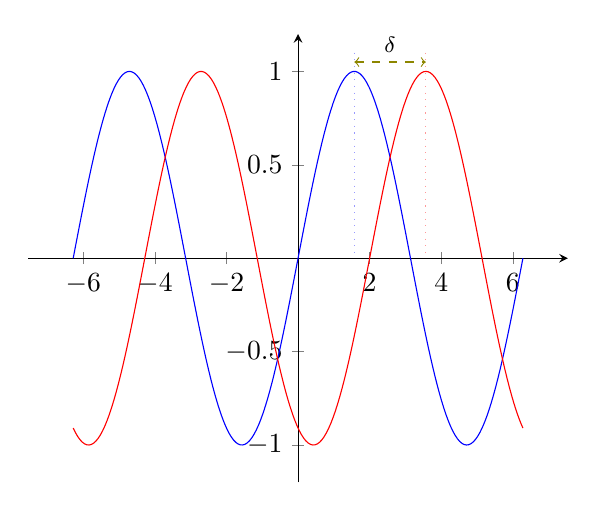
\begin{tikzpicture}
	  	\begin{axis}[
	    trig format plots=rad,
	    axis lines = middle,
	    enlargelimits,
	    clip=false
	    ]
	    \addplot[domain=-2*pi:2*pi,samples=200,blue] {sin(x)};
	    \addplot[domain=-2*pi:2*pi,samples=200,red] {sin(x-2)};
	    \draw[dotted,blue!40] (axis cs: 0.5*pi,1.1) -- (axis cs: 0.5*pi,0);
	    \draw[dotted,red!40] (axis cs: 0.5*pi+2,1.1) -- (axis cs: 0.5*pi+2,0);
	    \draw[dashed,olive,<->] (axis cs: 0.5*pi,1.05) -- node[above,text=black,font=\footnotesize]{$\delta$}(axis cs: 0.5*pi+2,1.05);
	  	\end{axis}
		\end{tikzpicture}
	\end{figure}
	\end{tcolorbox}
	Using the properties of trigonometric functions:
	
	
	Depending on we sum or subtract the this gives us the "\NewTerm{Euler formulas}" or "\NewTerm{de Moivre and Euler formulas}\index{de Moivre and Euler formulas}\label{de Moivre and Euler formulas}":
	\begin{equation}
	  \addtolength{\fboxsep}{5pt}
	   \boxed{
	   \begin{gathered}
	   	\begin{aligned}
		\cos(\varphi)&=\dfrac{e^{\mathrm{i}\varphi}+e^{-\mathrm{i}\varphi}}{2}\\
		\sin(\varphi)&=\dfrac{e^{\mathrm{i}\varphi}-e^{-\mathrm{i}\varphi}}{2\mathrm{i}}\\
	 	\end{aligned}
	   \end{gathered}
	   }
	\end{equation}
	Note that the angle can be a purely a complex number! This is to say that in all  generality trigonometric functions can be considered as functions that go from $\mathbb{C}$ to $\mathbb{C}$.
	
	A well known special case for the formulas above is the case where $\varphi=\pi$ and $r=1$. Then we have:
	
	after rearranging we get the famous geek relation:
	
	Another famous geek case is when we take still $r=1$ but with $\varphi=\pi/2$ and we raise to the power of $\mathrm{i}$. Then we get:
	
	and if we raise that to the power of $\mathrm{i}$:
	
	Some people consider then as a curious fact that $\mathrm{i}$ raised to the $\mathrm{i}$-th power is actually a real number.
	
	Thanks to the exponential form of a complex number, very commonly used in many fields of physics and engineering, we can easily draw relations such that starting from (remember that $\text{cis}$ is an old notation that stands for the $\cos(\varphi)+\mathrm{i}\sin(\varphi)$ being in the parenthesis):
	
	and assuming known the basic trigonometric identities (\SeeChapter{see section Trigonometry page \pageref{remarkable trigonometric identities}}) we have the following relations for the multiplication of two complex numbers:
	
	therefore:
	
	and therefore if $n$ is a positive integer:
	
	For the module (norm) of the multiplication:
	
	Therefore:
	
	For the division of two complex numbers:
	
	The module of their division then comes immediately:
	
	therefore we have for the argument:
	
	and it comes immediately:
	
	For the power of a complex number (or root):
	
	which gives us immediate a already proved previously:
	
	and for the argument:
	
	In case we have a unit module (norm equal to $1$) as $z=\cos(\varphi)+\mathrm{i}\sin(\varphi)$ we then have the relation:
	
	named "\NewTerm{de Moivre formula}\index{de Moivre formula}".

	For the natural logarithm of a complex number, we trivially have the following relation which is discussed in the section of Functional Analysis (page \pageref{logarithms}):
		
	where $\ln(z)$ is often in the complex case written $\mathrm{Log}(z)$ with an uppercase "L".
	
	All previous relations could of course be obtained with the trigonometric form of complex numbers but then require some additional lines of mathematical developments.
	
	\subparagraph{Fresnel Vectors (phasors)}\mbox{}\\\\
	A sinusoidal variation $f(t)=r\sin(\omega t)$ can be represented as the projection (\SeeChapter{see section Trigonometry page \pageref{trigonometry}}) on the vertical $y$-axis (imaginary axis the set $\mathbb{C}$) of a rotating vector $\vec{r}$ at angular velocity $\omega$ around the origin in the plane $x\text{O}y$:
	\begin{figure}[H]
		\centering
		\includegraphics{img/arithmetics/fresnel_representation.jpg}
		\caption{Fresnel representation}
	\end{figure}
	Such a rotating vector is named "\NewTerm{Fresnel vector}\index{Fresnel vector}" and can be well interpreted as the imaginary part of a complex number given by:
	
	That is to say:
	\begin{figure}[H]
		\centering
		\includegraphics{img/arithmetics/fresnel_rotating_vector.jpg}
		\caption{Fresnel rotating vector}
	\end{figure}
	We will see the phasor again explicitly in our study of wave mechanics and geometrical optics (as part of diffraction) in the sections with the corresponding names page \pageref{wave mechanics} and page \pageref{geometrical optics}.
	
	\paragraph{Transformation in the plane}\mbox{}\\\\	
	It is customary to represent real numbers as points on a graduated line. The algebraic operations have their geometric interpretation on it: the addition is a translation, a multiplication a centered scaling.
	
	In particular we can talk about the "square root of a transformation." A translation of amplitude $T$ may be obtained as the iteration of a translation of amplitude $T / 2$. Similarly, a scaling of amplitu $S$ can be achieved as iterated scaling of faction $\sqrt{S}$. In particular an homothety (scaling) of a factor $9$ can be composed of two homotheties (scaling) of respectively $3$ (or $-3$).
	
	Then we can say that the square root takes on a geometric sense. But what about the square root of negative numbers? In particular of the square root of $-1$???
	
	A scaling of factor $-1$ can be seen as a symmetry with respect to the origin. But if we see this transformation in a continuous manner. Therefore a $-1$ scaling factor also be seen as rotation of $\pi$ rotation around the origin.
	
	So, the problem of negative square root is simplified. Indeed, it is not difficult to break down a rotation of $\pi$ radians inot two transformations: we can repeat either a rotation of $\pi/2$ or of $-\pi/2$. The image of $1$ is the square root of $-1$ and $\mathrm{i}$ is situated on a perpendicular to the origin at a distance $1$ either up or down.
	
	Having successfully positioned the number $\mathrm{i}$ it not difficult anymore to put other complex numbers in the Gauss plane. We can therefore associate to $2\mathrm{i}$ the product of the scaling of a factor $2$ (\SeeChapter{see section Euclidean Geometry page \pageref{scaling}}) by the rotation of center O with angle of $\pi/2$, that is to say a similitude centered at the origin. This is what we will endeavor to prove now.
	
	Given:
	
	We have the following geometric transformations properties for complex numbers (see the section Trigonometry for the properties of sine and cosine) that we can happily combine at our discretion:
	\begin{enumerate}
		\item[P1.] The multiplication of $z_1$ by a real number $\lambda$ in the Gauss plane corresponds trivially to a homothety of center O (the intersection of real and imaginary axis for recall...) and of ration $\lambda$.
		
		Indeed:
		
		
		\item[P2.] Multiplying of $z_1$ by a complex number of unit module corresponds a rotation of center O and of angle corresponding to the argument of $z_1$. Indeed:
		
		\begin{tcolorbox}[title=Remark,colframe=black,arc=10pt]
		Then we see immediately, for example, that multiplying a complex number by $\mathrm{i}$ (that is to say a complex number with $ \sin(\omega)=1,\cos(\omega)=0$) corresponds a rotation of $\pi/2$
		\end{tcolorbox}
		\begin{theorem}
		It is interesting to notice that in vector form the rotation of center O of $z_1$ by $z_0$ can be written using the following matrix:
		
		\end{theorem}
		\begin{dem}
		We have just seen before that $z_0z_1$  is a rotation of center O of and angle $\omega$. We just need to write it first in the old style:
		
		giving in vector form:
		
		thus the linear equivalent application is:
		
		or as well (we fall back on the rotation matrix in the plane that we will see in the section of Euclidean Geometry page \pageref{rotation matrix in the plane} which is a remarkable result!) using:
		
		and in the particular and arbitrary case where $r$ is unitary (in order to have a pure rotation!):
		
		we have immediately (we took again the same notations for the angle as the one we we have in the chapter Geometry):
		
		Notic that the 2D rotation matrix can also be written as\label{2d rotation matrix}:
		
		as well:
		
		\begin{flushright}
			$\square$  Q.E.D.
		\end{flushright}
		\end{dem}
		Thus we see that the rotation matrices are not only applications but also are complex numbers (well it was obvious from the start but we had to show it in an aesthetic and simple way).
		
		So, we have for usage to put that:
		
		or with another common notation in linear algebra:
		
		The field of complex numbers is isomorphic to the field of real square matrices of dimension $2$ of the type:
		
		It is a result that we use many times in various sections of this book for specific studies in algebra, geometry and relativistic quantum physics.
		
		\item[P3.] The multiplication of two complex corresponds to a homothety added to a rotation. In other words, a "\NewTerm{direct similarity}\index{direct similarity}".
		\begin{dem}
		
		so this is indeed a similarity of ratio $b$ and angle $\beta$.
		
		At the opposite, the following operation:
		
		will be named a "\NewTerm{retrograde linear similarity}\index{retrograde linear similarity}".
		
		Otherwise, it returns trivially an already known following relation:
		
		\begin{tcolorbox}[title=Remarks,colframe=black,arc=10pt]
		\textbf{R1.} As the sum of two complex numbers $z_1+z_2$ can not have a special simplified mathematical notation in any form whatsoever, then we say that the resulting quantity is equivalent to an "\NewTerm{amplitude translation}\index{amplitude translation}".\\
		
		\textbf{R2.} The combination of a direct linear similarity (multiplication of two complex numbers) and an amplitude translation (sum by a third complex number) is what we name a "\NewTerm{direct linear similarity}\index{direct linear similarity}".
		\end{tcolorbox}
		\begin{flushright}
			$\square$  Q.E.D.
		\end{flushright}
		\end{dem}
		
		\item[P4.] The conjugate of a complex number is geometrically symmetrical with respect to the axis such that:
		
		without forgetting that (basis of trigonometry):
		
		This gives us a known result:
		
		From which we get the following property:
		
		Hence:
		
		
		\item[P5.] The negation of the conjugate of a complex number is geometrically its symmetrical with respect to the imaginary axis such that:
		
		\begin{tcolorbox}[title=Remarks,colframe=black,arc=10pt]
		\textbf{R1.} The combination of the properties P4, P5 is named a "\NewTerm{retrograde similarity}\index{retrograde similarity}".\\
		
		\textbf{R2.} The geometric operation that consist to take the inverse of the conjugate of a complex number (that is to say $\bar{z}^{-1}$) is named a "\NewTerm{pole inversion}\index{pole inversion}".
		\end{tcolorbox}
		
		\item[P6.] The rotation of coordinate cente $c$ and angle $\varphi$ is given and denoted by:
		
		Some explanations could be useful for some readers:
		
		The complex $c$ gives a point in the Gaussian plane, which will be the center of rotation. The difference $z_1-c$ gives the chosen radius $r$. The multiplication by $e^{\mathrm{i}\varphi}$ is the counterclockwise rotation of the radius from the origin of the Gaussian plane. Finally, the addition by $c$ is the necessary translation to take back the rotated radius $r$ at its original place before the rotation (center $c$). Which gives schematically:
		\begin{figure}[H]
			\centering
			\includegraphics{img/arithmetics/complex_rotation.jpg}
			\caption{Representation of the complex rotation}
		\end{figure}
	
		\item[P7.] On the same idea, we get and denote an homothety of center $c$ and ratio $\lambda$ by:
		
		Some explanations could be useful for some readers:
		
		The difference $z_1-c$ always gives the radius $r$ and $c$ a central point in the Gauss plane. The expression $\lambda(z_1-c)$ gives the homothety of the radius from the origin of the Gaussian plane, and finally by adding $c$ gives the necessary translation for the homothety to be see as being made from center $c$.
	\end{enumerate}
	
	\subsubsection{Quaternion Numbers}\label{quaternions}
	Also named "\NewTerm{hypercomplex}\index{hypercomplex}" quaternions numbers were invented in 1843 by William Rowan Hamilton to generalize complex numbers.
	
	\textbf{Definition (\#\mydef):} A "\NewTerm{quaternion}\index{quaternion}" is an element $(a,b,c,d)\in \mathbb{R}^4$ and for which we denote by $\mathbb{H}$ the set that contains it and what we name the "\NewTerm{set of quaternions}\index{set of quaternions}".
	
	A quaternion can also be represented in a row or column such as:
	
	We define the sum of two quaternions $(a, b, c, d)$ and $(a ', b', c ', d')$ by:
	
	\begin{tcolorbox}[title=Remark,colframe=black,arc=10pt]
	It is the natural addition in $\mathbb{R}^4$ seen as a $\mathbb{R}$-vector space (\SeeChapter{see section Set Theory page \pageref{vector space}}).
	\end{tcolorbox}
	The associativity is verified by applying the corresponding properties of the operations on $\mathbb{R}$.
	
	We also define the multiplication:
	
	of two quaternions $(a, b, c, d)$ and $(a', b', c', d')$ by the expression:
	
	It may be hard to accept but we will be a little further below that there is a family resemblance with the complex numbers.
	
	We can notice that the law of multiplication is not commutative. Indeed, taking the definition of the multiplication above, we have:
	
	But we can also notice that:
	
	\begin{tcolorbox}[title=Remark,colframe=black,arc=10pt]
	It is the natural multiplication in $\mathbb{R}^4$ seen as a $\mathbb{R}$-vector space (\SeeChapter{see section Set Theory page \pageref{vector space}}).
	\end{tcolorbox}
	The law of multiplication is distributive with the addition law but it is an excellent example where we must still be careful to prove the left and right distributivity, since the product is not commutative!
	
	The multiplication have for neutral element:
	
	Indeed:
	
	Any element:
	
	is inversible.
	
	Indeed, if $(a,b,c,d)$ is a non-null quaternion, we then have necessarily:
	
	otherwise the four numbers $a, b, c, d$ are of square null, so all zero. Given then the quaternion $(a_1,b_1,c_1,d_1)$ defined by:
	
	then by applying mechanically  the definition of the multiplication of quaternions, we check that:
	
	this latter quaternion is therefore the inverse for the multiplication!
	
	Let us prove (for general knowledge) that the field of complex numbers $(\mathbb{C},+,\times)$ is a subfield of $(\mathbb{H},+,\times)$.
	\begin{tcolorbox}[title=Remark,colframe=black,arc=10pt]
	We could also have put this proof in the section of  Set Theory because we will make use of a lot of concepts that are have seen there but it seemed to us a little more relevant to put instead the proof here. We expect the reader to tolerate this choice.
	\end{tcolorbox}
	Given $\mathbb{H}'$ set set of quaternions of the form $(a, b, 0,0)$. If $\mathbb{H}'$ is not empty, and if $(a, b, 0,0)$, $(a ', b', 0.0)$ are elements $\mathbb{H}'$ the $(\mathbb{H}',+\times)$ is a field. Indeed:
	\begin{enumerate}
		\item[P1.] For subtraction (and therefore the addition):
		

		\item[P2.] The multiplication:
			

		\item[P3.] The neutral element:
		

		\item[P4.] And finally the inverse:
		
		of $(a,b,0,0)$ is still in.
	\end{enumerate}
	Therefore $(\mathbb{H}',+,\times)$ is a subfield of $\mathbb{H}$. Given then the application:
	
	$f$ is bijective, and we easily check that for any complex $z_1,z_2$, we have:
	
	Therefore $f$ is an isomorphism of $(\mathbb{C},+,\times)$ on $(\mathbb{H}',+,\times)$.
	
	This isomorphism has for interest (caused) to identify $\mathbb{C}$ to $\mathbb{H}'$ and to write $\mathbb{C} \subset\mathbb{H}$, the laws of addition and subtraction on $\mathbb{H}$ extending the already known operations of $\mathbb{C}$.
	
	Thus, by convention, we will write any element of $(a, b, 0,0)$ of $\mathbb{H}'$ in the complex form $a + \mathrm{i}b$. Particularly $0$ is the element $(0,0,0,0)$, $1$ is the element $(1,0,0,0)$ and $\mathrm{i}$ and the element $(0,1,0,0)$.
	
	We denote by analogy and by extension $\mathrm{j}$ the element $(0,0,1,0)$ and $\mathrm{k}$ the element $(0,0,0,1)$. The family $\{1, \mathrm{i}, \mathrm{j}, \mathrm{k}\}$ form a basis of all quaternions seen as a vector space on $\mathbb{R}$, and we will write:
	
	the quaternion $(a, b, c, d)$.

	The notation of quaternions as defined above is perfectly suited to the multiplication operation. For the product of two quaternions we get by developing the expression:
	
	$16$ terms that we have to identify to the original definition of multiplication of quaternions to get the following relations:
	
	Which can be summarized in a table:
	
	We can see that the expression of the multiplication of two quaternions looks partly much like a vector product (denoted $\times$ in this book) and dot product (denoted $\circ$ in this book):
	
	If this is not evident (which would be quite understandable), let make a concrete example:
	\begin{tcolorbox}[colframe=black,colback=white,sharp corners]
	\textbf{{\Large \ding{45}}Example:}\\\\
	Given two quaternions without real part:
	
	and $\vec{u},\vec{v}$  the vectors of $\mathbb{R}^3$ of respective components $(x,y,z)$ and $(x',y',z')$. Then the product:
	
	is equal to:
	
	We can also for curiosity interest us to the general case ... Given for this two quaternions:
	
	Then we have:
	
	\end{tcolorbox}
	\textbf{Definition (\#\mydef):} The center of the non-commutative field $(\mathbb{H},+,\times)$ is the set of elements of $\mathbb{H}$ commuting for the law of multiplication with all the elements of $\mathbb{H}$.

	\begin{theorem}
	The center of $(\mathbb{H},+,\times)$ is the set of real numbers!
	\end{theorem}
	\begin{dem}
Give $\mathbb{H}_1$ is the center of $(\mathbb{H},+,\times)$, and $(x, y, z, t)$ a quaternion. We must have the following conditions are met:

	Given $(x,y,z,t)\in \mathbb{H}_1 $ then for any $(a,b,c,d)\in \mathbb{H}$ we seek:
	
	which give by developing:
	
	after simplification (the first line of the previous system is equal to zero on both sides of equality):
	
	the resolution of this system gives us:
	So that the quaternion $(x, y, z, t)$ is the center of  $\mathbb{H}$ it must be real (not imaginary parts)!
	\begin{flushright}
		$\square$  Q.E.D.
	\end{flushright}
	\end{dem}
	Just as for complex numbers, we can define a conjugate of quaternions:
	
	\textbf{Definition (\#\mydef):} The conjugate of a quaternion $Z=(a,b,c,d)$ is the quaternion $\bar{Z}=(a,-b,-c,-d)$.

	Just as for the complex number, we notice that:
	\begin{enumerate}
		\item First clearly that if $Z=\bar{Z}$ then it means that $Z\in \mathbb{R}$

		\item That $Z+\bar{Z}\in \mathbb{R}$

		\item That by developping the product $Z\bar{Z}$ we have:
		
		that we will adopt, by analogy with complex numbers, as a definition of the norm (or module) of quaternions such as:
		
		Therefore we also have immediately (relation which will be useful later):
		
	\end{enumerate}
	As for complex numbers (see below), it is easy to show that the conjugation is an automorphism of the group $(\mathbb{H},+)$.
	
	It is also easy to prove that it is involutive. Indeed:
	
	But the conjugation is not a multiplicative automorphism of the field $(\mathbb{H},+,\times)$. Indeed, if we consider the multiplication of $Z$, $\bar{Z'}$ and take the conjugate:
	
	we see immediately (at least for the second row) that we have:
	
	Let us now back to our norm (or module) .... For this, let us calculate the square of the norm $|ZZ'|$:
	
	We know (by definition) that:
	
	Let us denote this product in such a way that:
	
	Then we have:
	
	substituting it comes:
	
	after an elementary algebraic development (frankly boring) we find:
	
	Therefore:
	
	\begin{tcolorbox}[title=Remark,colframe=black,arc=10pt]
	The norm is therefore a homomorphism of $(\mathbb{H},\times)$ in $(\mathbb{R},\times)$. Subsequently, we will denote by $\mathbb{G}$ all the quaternions of unit norm.
	\end{tcolorbox}
	
	\paragraph{Matrix Interpretation of Quaternions}\mbox{}\\\\
	Given $q$ and $p$ two quaternions and given the application:
	
	The  (left) multiplication can be made with a linear application (\SeeChapter{see section Linear Algebra page \pageref{linear application}}) on $\mathbb{H}$.
	
	If $q$ is written:
	
	this application has for matrix in the basis $(1,\mathrm{i},\mathrm{j},\mathrm{k})$:
	
	What we check well:
	
	In fact, we can then define the quaternions as the set of matrices with the visible structure above if we wanted to. This will then reduce them to a sub vector space of $M_4(\mathbb{R})$.
	
	Especially, the matrix of $1$ (the real part of the quaternion $q$) is then nothing other than the identity matrix:
	
	as well:
	
	
	\paragraph{Rotations with Quaternions}\mbox{}\\\\
	We will see now that conjugation by an element of the group $\mathbb{G}$ of the quaternions of unit norm can be interpreted as a pure rotation in space!
	
	\textbf{Definition (\#\mydef):} The "\NewTerm{conjugation}\index{conjugation}" by a non-nul quaternion $q$ of unit norm is the application $S_q$ defined on $\mathbb{H}$ by:
	
	and we affirm that this application is a rotation.
	
	\begin{tcolorbox}[title=Remarks,colframe=black,arc=10pt]
	\textbf{R1.} As $q$ is of unit norm $1$, we have obviously $|q|=q\bar{q}=1$ therefore $q^{-1}=\bar{q}$. This quaternion can be seen as the proper value (of unit norm) to the application (matrix) $p$ on the vector $\bar{q}$ (we are in a similar situation as the orthogonal rotation matrices seen in the section of Linear Algebra page \pageref{orthogonal matrix}).\\
	
	\textbf{R2.} $S_q$ is a linear application (so if it is rotation, the rotation can be decomposed into several rotations). Indeed, let consider two quaternions $p_1,p_2$ and two real number $\lambda_1,\lambda_2$, then we have:
	
	\end{tcolorbox}
	Let us now check that the application is indeed a pure rotation. As we saw in our study of Linear Algebra and in particular of orthogonal matrices (\SeeChapter{see section Linear Algebra page \pageref{orthogonal matrix}}), a first obvious condition is that the application conserves the norm.
	
	Let us check this:
	
	Moreover, we can check that a rotation of a purely complex quaternion (such that then we restrict ourselves to $\mathbb{R}^3$) and the same summed reverse rotation is zero (the vector sum up to its opposite cancel):
	
	we trivially check that if we have two quaternions $q, p$ then $\overline{p\cdot q}=\bar{q}\bar{p}$ since then:
	
	for this operation to be zero, we immediately see that we need to restrict ourselves to the purely complex quaternions $p$. Since then:
	
	We conclude then that $p$ must be purely complex so the for the application $S_q$ is a rotation and that $S_q(p)$ is a pure quaternion. In other words, this application is stable (in other words: a pure quaternion by this application remains a pure quaternion).
	
	The application $S_q$ restricted to all purely complex quaternions is thus a vectorial isometry, that is to say a symmetry or a rotation.
	
	We have also seen during our study of the rotation matrices in the section of Linear Algebra page \pageref{rotation matrix in linear algebra} and Euclidean Geometry page \pageref{rotation matrix in the plane} that such matrices should have a determinant equal to $+1$ so that we have a rotation. Let's see if this is the case of $S_q$:
	
	For this, we explicitly calculate in function of:
	
	the matrix (in the canonical basis $(\mathrm{i},\mathrm{j},\mathrm{k})$) of $S_q$ and we calculate its determinant. Thus we obtain the coefficients of the columns of this application by remembering that:
	
	and then by calculating:
	
	
	
	
	
	We must then calculate the determinant of the following matrix (pfff ...):
	
	remembering that (which also simplifies the expression of the terms of the diagonal as we can see in some books):
	
	we find that the determinant is indeed equal to $1$. Otherwise, we can check this with Maple 4.00b:
	
	\texttt{>with(linalg):\\
	>A:=linalg[matrix](3,3,[a\string^2+b\string^2-c\string^2-d\string^2,2*(a*d+b*c),\\
	2*(b*d-a*c),2*(b*c-a*d),a\string^2-b\string^2+c\string^2-d\string^2,2*(a*b+c*d),\\
	2*(a*c+b*d),2*(c*d-a*b),a\string^2-b\string^2-c\string^2+d\string^2]);\\
	>factor(det(A));}
	
	Let us now show that this rotation is a half axis turn (the example that may seem particular is in fact general!):
	
	First, if:
	
	we have:
	
	which means that the axis of rotation $(x, y, z)$ is fixed by the application $S_q$ itself!
	
	On the other hand, we have seen that if $q$ is a purely complex quaternion of norm $1$ then:
	
	Which gives us the relation:
	
	This result leads us to calculate the rotation of a rotation:
	
	Conclusion: Since the rotation of a rotation is a full turn, then $S_q$ is necessarily a half-turn:
	
	relatively (!) to the axis $(x, y, z)$.
	
	At this stage, we can say that any rotation of the space can be represented by $S_q$ (the conjugation by a quaternion $q$ of norm $1$). Indeed, the half turns generates the group of rotations, that is to say that any rotation can be expressed as the product of a finite number of half-turns, and therefore by conjugation of a product of quaternions unitary norm (product which is itself a quaternion of unitary norm...).
	
	We will still give an explicit form connecting a rotation and the quaternion that represents it, just as we did for complex numbers.
	\begin{theorem}
	Given $\vec{u}(x,y,z)$ a unit vector and $\theta \in [0,2\pi]$ angle. The we affirm that the rotation of axis $\vec{u}$ and angle $\theta$ corresponds to the application $S_q$, where $q$ is the quaternion:
	
	For this assertion is verified, we know we need that: 
	\begin{itemize}
		\item The norm of $q$ is equal to $1$

		\item The determinant of the application $S_q$ is equal to $1$

		\item The application $S_q$ conserves the norm
	
		\item The application $S_q$ returns all collinear vector to the axis of rotation on the axis of rotation itself.
	\end{itemize}
	\end{theorem}
	\begin{dem}
	Ok let us check every point:
	\begin{enumerate}
		\item The norm of the quaternion previously proposed is indeed equal to $1$:
		
		and as $\vec{u}(x,y,z)$ is of unit norm, we have:
		
		Therefore:
		
		
		\item The fact that $q$ is a quaternion of unit norm  immediately leads to the fact that the determinant of the application $S_q$ is also equal to $1$. We have already proved it above in the general case of any quaternion of norm $1$ (necessary and sufficient condition).
		
		\item It is the same for the conservation of the norm. We have already proved earlier above that this was the case anyway when the quaternion $q$ of norm $1$ (necessary and sufficient condition).

		\item Let us now prove that all collinear vector to the axis of rotation is projected onto the axis of rotation itself. Let us denote by $q'$ the purely imaginary unitary quaternion $xi+yj+zk$. Then we have:
		
		Then:
		
		but as $q'$ is the restriction of $q$ to the pure elements that constitute it, this is equivalent as to write:
		
		Let us now show why we choose the writing $\theta/2$. If $\vec{v}=(x_1,y_1,z_1)$ denotes a unit vector orthogonal to $\vec{u}$ (therefore perpendicular to the axis of rotation), and $p$ the quaternion $x\mathrm{i}+y\mathrm{j}+z\mathrm{k}$ then we have:	
		
		We have shown during the definition of multiplication of two quaternions that:
		
		therefore we get:
		
		We have also prove earlier above that:
		
		Therefore:
		
		(the half turn of axis $(x, y, z)$). So:
		
		\begin{tcolorbox}[title=Remark,colframe=black,arc=10pt]
		We are beginning to see here already the usefulness of having chose from the beginning $\theta/2$ for the angle!
		\end{tcolorbox}
	\end{enumerate}
	\begin{flushright}
		$\square$  Q.E.D.
	\end{flushright}
	\end{dem}
	We know that $p$ is the pure quaternion likened to a unit vector $\vec{v}$ orthogonal to the axis of rotation $\vec{u}$ itself equated withthe purely imaginary part of $q'$. We notice then immediately that  the imaginary part of the product (defined!) of the quaternion $q'p$ is equal to the cross product $\vec{u}\times\vec{v}=\vec{w}$. This vector product therefore generates a vector perpendicular to $\vec{u},\vec{v}$.
	
	The pair $(\vec{v},\vec{w})$ thus form a plane perpendicular to the axis of rotation $\vec{u}$ (that's as for the simple complex numbers $\mathbb{C}$ in which we have the Gaussian plane and perpendicular to it the axis of rotation!).
	
	Then finally:
	
	We fall back with on rotation based on a plane (but therefore be in space!) identical to that shown earlier above with the standard complex numbers $\mathbb{C}$ in the Gaussian plane. For more details the reader can refer the  section of Spinor Calculus page \pageref{spinors}.
	
	So we know how to do any kind of rotation in space in a single mathematical operation and with a bonus: with the free choice of the axis!

	We can now better understand why the algebra of quaternions is not commutative. Indeed, the vector rotations of the plan are commutative but those of space are not like show us the example below:
	
	Given the initial configuration:
	\begin{figure}[H]
		\centering
		\includegraphics{img/arithmetics/quaternion_initial_configuration.jpg}
		\caption[]{Starting situation for quaternion rotations}
	\end{figure}
	Then a rotation about the $X$-axis followed by a rotation around the $Y$ axis:
	\begin{figure}[H]
		\centering
		\includegraphics{img/arithmetics/quaternion_x_y_rotation.jpg}
		\caption[]{Example quaternion $X-Y$ rotation}
	\end{figure}
	is not equal to a rotation around the $Y$-axis followed by a rotation about the axis $X$:
	\begin{figure}[H]
		\centering
		\includegraphics{img/arithmetics/quaternion_y_x_rotation.jpg}
		\caption[]{Example of non-equivalence for quaternion rotation }
	\end{figure}
	The results will be fundamental for our understanding of spinors (\SeeChapter{see section Spinor Calculus page \pageref{spinors}})!
	
	\subsubsection{Algebraic and Transcendental Numbers}
	\textbf{Definitions (\#\mydef):}
	\begin{enumerate}
		\item[D1.] We name "\NewTerm{algebraic integer of degree $n$}\index{algebraic integer of degree $n$}", any complex number that is a solution of an univariate algebraic equation of degree $n$, ie a polynomial of degree $n$ (concept that we will discuss in the chapter of Algebra) whose coefficients are integers and whose dominant coefficient is equal to $1$.

		\item[D2.] We name "\NewTerm{algebraic number of degree $n$}\index{algebraic number of degree $n$}", any complex number that is a solution of an univariate algebraic equation of degree $n$, ie a polynomial of degree $n$ whose coefficients are rational.
	\end{enumerate}
	
	The set of algebraic number is sometimes denoted by $\overline{\mathbb{Q}}$ or $\mathbb{A}$.
	
	\pagebreak
	\begin{theorem}
	A first interesting result and particularly in this area of study (mathematical curiosity ...) is that a rational number is an "algebraic integer of degree $n$" if and only if it's an integer (read several times need...). In scientific terms, we the say that the ring $\mathbb{Z}$ is "\NewTerm{fully closed}\index{fully closed ring}".
	\end{theorem}
	\begin{dem}
	We will assume that the number $p/q$ , where $p$ and $q$ are two prime integers (that is to say that their ratio does not give an integer or more rigorously ... that the greatest common divisor of $p,q$ is equal to $1$! , is a root of the following polynomial (\SeeChapter{see section Calculus page \pageref{polynomial}}) with relativer integer coefficients ($\in\mathbb{Z}$) and whose dominant coefficient is equal to $1$:
	
	where the equality with zero of the polynomial is implicit.
	
	In this case:
	
	Since the coefficients are by definition all integers and their multiple in the parenthesis also, then the parenthesis has necessarily a value in $\mathbb{Z}$.
	
	Therefore, $q$ (at the right of the parenthesis) divides a power of $p$ (at the left of the equality), which is possible, in the set $\mathbb{Z}$ (because our bracket has a value in this same set for recall...), only if $q$ is equal to $\pm 1$ (as they were prime together).
	
	So among all rational numbers the only that are solutions of polynomial equations with relative integer coefficients $(\in \mathbb{Z}$) for which the dominant coefficient is equal to $1$ are relative integers!
	\begin{flushright}
		$\square$  Q.E.D.
	\end{flushright}
	\end{dem}
	To take another interesting and particular case, it is easy to show that any rational number is an algebraic number. Indeed, if we take the simplest following univariate polynomial:
	
	where $p$ and $q$ are relatively prime and where $q$ is different from $1$. So as this is a simple polynomial with rational coefficients ($\in\mathbb{Q}$), after remaniment we have:
	
	So since $p$ and $q$ are relatively prime and $q$ is different from $1$, we have indeed that every rational number is an "algebraic number of degree $1$".
	
	We also have the real (and irrational) number $\sqrt{2}$ which is an "algebraic integer of degree $2$" because it is the root of:
	
	and the complex number $\mathrm{i}$ is also an "algebraic integer of degree $2$" because it is the root of the equation:
	
	etc.
	
	\textbf{Definition (\#\mydef):} A "\NewTerm{transcendental number}\index{transcendant number}" is a real or complex number that is not algebraic. That is, it is not a root of a non-zero polynomial equation with rational coefficients.
	
	\begin{theorem}
	The set of all transcendental numbers is uncountable. The proof is simple and requires no difficult mathematical development.
	\end{theorem}
	\begin{dem}
	Indeed, since the polynomial with integer coefficients are countable, and since each of these polynomials has a finite number of roots (see the Factorization Theorem in the section Calculus page \pageref{factorization theorem}), the set of algebraic numbers is countable! But the argument of Cantor's diagonal (\SeeChapter{see section Set Theory page \pageref{Cantor's diagonal}}) states that real numbers (and therefore also the complex numbers) are uncountable, so the set of all transcendental numbers must be uncountable.
	
	In other words, there is much more transcendental numbers than algebraic numbers...
	\begin{flushright}
		$\square$  Q.E.D.
	\end{flushright}
	\end{dem} 
	The best known transcendent numbers are $\pi$ and $e$. We are still looking to provide you a proof more nice and intuitive than that of Hilbert or  Lindemann–Weierstrass.
	
	Here is a small summary of all the stuff see until now:
	\begin{figure}[H]
		\centering
		\includegraphics{img/arithmetics/numbers_type.jpg}
		\caption{Numbers Type $\mathbb{N},\mathbb{Z},\mathbb{Q},\mathbb{R},\mathbb{C},$...}
	\end{figure}
	
	\pagebreak
	\subsubsection{Universe Numbers (normal numbers)}
	\textbf{Definition (\#\mydef):} A "\NewTerm{Universe number}\index{Universe number}" also named "\NewTerm{normal number}\index{normal number}" is a real number whose infinite sequence of digits in every base $b$ is distributed uniformly in the sense that each of the $b$ digit values has the same natural density $1/b$. Intuitively this means that no digit, or (finite) combination of digits, occurs more frequently than any other. The set of Universe numbers is sometimes denoted $\mathbb{U}$.

	While a general proof can be given that almost all purely real numbers are Universe numbers \cite{filip2010elementary} this proof is not constructive and only very few specific numbers have been shown to be Universe numbers. It is widely believed that the (computable) numbers $\sqrt{2}$, $\pi$, and $e$ are Universe numbers, but a proof remains elusive still in this year 2016. All of them however are strongly conjectured to be because of some empirical evidence. It is not even known whether all digits occur infinitely often in the decimal expansions of those constants. In particular, the popular claim "every string of numbers eventually occurs in $\pi$" or "the whole Holy book is contained in $\pi$ is not known to be true. It has been conjectured that every irrational algebraic number is a Universe number, while no counterexamples are known, there also exists no algebraic number that has been proven to be a Universe number in any base.
	
	More formally, let $\sum$ be a finite alphabet of $b$ digits, and $\sum^\infty$ the set of all sequences that may be drawn from that alphabet. Let $S\in\sum^\infty$ be such a sequence. For each $a$ in $\sum$ let $N_S(a, n)$ denote the number of times the letter a appears in the first $n$ digits of the sequence $S$. We say that $S$ is a "\NewTerm{simple Universe number}\index{simple Universe number}" if the limit:
	
	for each $a$. 

	Now let $w$ be any finite string in $\sum^{*}$ and let $N_S(w, n)$ to be the number of times the string $w$ appears as a substring in the first $n$ digits of the sequence $S$ (for instance, if $S = 01010101$..., then $N_S(010, 8) = 3$). Then $S$ is a "\NewTerm{Universe number}\index{Universe number}" if, for all finite strings $w\in \sum^{*}$:
	
	$S$ is therefore a Universe number if all strings of equal length occur with equal asymptotic frequency. A given infinite sequence is either a Universe number or not, whereas a pure real number, having a different base-$b$ expansion for each integer $b\geq 2$, may be a Universe number in one base but not in another. A "\NewTerm{disjunctive sequence}\index{disjunctive sequence}" is a sequence in which every finite string appears. A Universe number sequence is a "\NewTerm{disjunctive sequence}\index{disjunctive sequence}" but a disjunctive sequence need obviously not be a Universe number.
	
	It is possible to prove (yet we don't wish not present this proof in a book on applied mathematics) with the "Universe number theorem" that almost all pure real numbers are Universe number. The set of non-Universe numbers, though "small" in the sense of being a null set, is "large" in the sense of being uncountable (for example o rational number is normal to any base, since the digit sequences of rational numbers are eventually periodic!). For instance, there are uncountable many numbers whose decimal expansion does not contain the digit $5$, and none of these are Universe number.
	
	\pagebreak
	\subsubsection{Abstract Numbers (variables)}
	\textbf{Definitions (\#\mydef):} A number may be considered as doing abstraction from the nature of the objects that constitute the group that it characterizes as well as how to codify it (Indian notation, Roman notation, etc.). We then say that the number is an "\NewTerm{abstract number}\index{abstract number}".  In other words, an abstract number, is a number that does not designate the quantity of any particular kind of thing.
	\begin{tcolorbox}[title=Remark,colframe=black,arc=10pt]
	Arbitrarily, the human being has adopted a numerical system mainly used in the World and represented by the symbols $0, 1, 2, 3, 4, 5, 7, 8, 9$ of the decimal system that will be supposedly known both in writing thant orally by the reader (language learning).
	\end{tcolorbox}
	For mathematicians, it is not advantageous to work with these symbols because they represent only specific cases. What seek theoretical physicists and mathematicians are "\NewTerm{literal relations}\index{literal relations}" applicable in a general case and that engineers can according to their needs change these abstract numbers by numeric values that correspond to the problem they need resolve.

These abstract numbers today commonly named "\NewTerm{variable}\index{variable}" or "\NewTerm{unknown}", used in the context of "\NewTerm{literal calculation}\index{literal calculation}" are very often represented since the $16$th century by:
	\begin{enumerate}
		\item The Latin alphabet:
		\begin{gather*}
			a,b,c,d,e,\ldots,x,y,z;A,B,C,D,E,\ldots, X,Y,Z
		\end{gather*}
		where the first lower case letters of the latin alphabet ($a, b, c, d, e ...$) are often used to represent an abstract constant, while the lowercase letters of the end of the latin alphabet ($...,x, y, z$) are used to represent entities (variables or unknowns) we seek the value.
		
		\item The Greek alphabet:
		\begin{table}[H]\centering\small
			\begin{tabular}{clcl}\hline
			A$\alpha$ & Alpha & $\Lambda \lambda$ & Lambda \\
			B$\beta$  & Beta  & M$\mu$ & Mu \\
			$\Gamma\gamma$ & Gamma & N$\nu$ & Nu \\
			$\Delta\delta$ & Delta & $\Xi\xi$ & Xi\\
			E$\varepsilon\varepsilon$ & Epsilon & O$o$ & Omicron\\
			Z$\zeta$ & Zeta & $\Pi\pi$ & Pi\\
			H$\eta$ & Eta & P$\rho$ & Rho \\
			$\Theta\theta\vartheta$ & Theta & $\Sigma\sigma$ & Sigma\\
			I$\iota$ & Iota & T$\tau$ & Tau \\
			K$\kappa$ & Kappa & $\Upsilon\upsilon$ & Upsilon \\
			$\Phi\phi\varphi$ & Phi & X$\chi$ & chi \\
			$\Psi\psi$ & Psi & $\Omega\omega$ & Omega \\ \hline
			\end{tabular}
			\caption{Greek Alphabet}
		\end{table}
		which is particularly used to represent more or less complex mathematical operators (such as the index sum $\Sigma$, the indexed product $\Pi$, the variational $\delta$, the infinitesimal element $\varepsilon$, partial differential $\partial$, etc.) or variables in the field of physics (as $\omega$ for the pulsation, $\nu$ for the frequency, $\rho$ for the density, etc.).
		
		\item The modernized Hebrew alphabet (with less intensity...)
		
		As we have seen, a transfinite cardinal for example is denoted by the letter "aleph": $\mathcal{N}_0$.
	\end{enumerate}
	Although these symbols can represent any number there are some who can represent physical constants also named "\NewTerm{Universal constant}\index{universal physical constant}" as the speed of light $c$, the gravitational constant $G$, the Planck constant $h$, the number $\pi$, etc.
	
	We use very often still other symbols that we will introduce and define when reading this book.
	\begin{tcolorbox}[title=Remark,colframe=black,arc=10pt]
	The letters to represent numbers had been used for the first time by Vieta in the $16$th century.
	\end{tcolorbox}
	
	\paragraph{Domain of a Variable}\mbox{}\\\\
	A variable is therefore likely to take different numerical values. All these values can vary according to the character of the problem considered. 
	
	Given two numbers $a$ and $b$ such that $a<b$, then:
	
	\textbf{Definitions (\#\mydef):}\label{domain of definition}
	\begin{enumerate}
		\item[D1.] We name "\NewTerm{domain of definition}\index{domain of definition}" of a variable, all numerical values it is likely to take between two specified limits (endpoints) or on a set (like $\mathbb{N}, \mathbb{R},\mathbb{R}^+,$ etc.).
		
		\item[D2.] We name "\NewTerm{closed interval with endpoints $a$ and $b$}\index{closed interval}", the set of all numbers $x$ between these two values and we denote as example as follows:
		
		The left notation is named obviously "\NewTerm{interval notation}\index{interval notation}", the right one is named "\NewTerm{setbuilder notation}\index{setbuilder notation}".
		
		\item[D3.] We name "\NewTerm{open interval with endpoints $a$ and $b$}\index{open interval}", the set of all numbers $x$ between these two values not included and we denote it as example as follows:
		
		
		\item[D4.] We name "\NewTerm{interval closed, left open right}\index{semi-interval}" or "\NewTerm{semi-closed left}" the following relation as example:
		
		
		\item[D5.] We name "\NewTerm{interval open left, closed right}\index{semi-interval}" or "\NewTerm{semi-closed right}" the following relation as example:
		
	\end{enumerate}
	Or in a summary and imaged  form and as often denoted in Switzerland:
	\begin{table}[H]
		\begin{center}
			\definecolor{gris}{gray}{0.85}
				\begin{tabular}{|c|c|c|p{6cm}|}
					\hline
					\multicolumn{1}{c}{\cellcolor{black!30}\textbf{Type}} & 
	  \multicolumn{1}{c}{\cellcolor{black!30}\textbf{Visual}} & 
	  \multicolumn{1}{c}{\cellcolor{black!30}\textbf{Math notation}} & 
	  \multicolumn{1}{c}{\cellcolor{black!30}\textbf{Explicitly}} \\ \hline
					$[a,b]$ & \cincludegraphics{img/arithmetics/domain_interval_1.jpg} & $a\leq x \leq b$ & Closed bounded interval\label{closed bounded interval} \\ \hline
					$[a,b[$ & \cincludegraphics{img/arithmetics/domain_interval_2.jpg} & $a\leq x < b$ & Semi-closed and bounded interval on $a$ and semi-open on $b$ (or left semi-closed and right semi-open)\\ \hline
					$]a,b]$ & \cincludegraphics{img/arithmetics/domain_interval_3.jpg} & $a< x \leq b$ & Semi-open bounded interval on $a$ and semi-closed on $b$ (or left semi-open and right semi-closed)\\ \hline
					$]a,b[$ & \cincludegraphics{img/arithmetics/domain_interval_4.jpg} & $a< x < b$ & Bounded open interval\\ \hline
					$]-\infty,b]$ & \cincludegraphics{img/arithmetics/domain_interval_5.jpg} & $ x \leq b$ & Unbounded interval closed on $b$ (or closed right) \\ \hline
					$]-\infty,b[$ & \cincludegraphics{img/arithmetics/domain_interval_6.jpg} & $ x \leq b$ & Unbounded interval open on $b$ (or open right) \\ \hline
					$[a,+\infty[$ & \cincludegraphics{img/arithmetics/domain_interval_7.jpg} & $a\leq x$ & Unbounded interval closed on $a$ (or closed left) \\ \hline
					$]a,+\infty[$ & \cincludegraphics{img/arithmetics/domain_interval_8.jpg} & $a< x $ & Unbounded interval open on $a$ (or open left) \\ \hline
			\end{tabular}
		\end{center}
		\caption{Resume of main Combinatorial Analysis cases}
	\end{table}
	and according to the international norm ISO 80000-2: 2009 (since Switzerland has the art not respecting international norms and standards):
	\begin{table}[H]
		\begin{center}
			\definecolor{gris}{gray}{0.85}
				\begin{tabular}{|c|c|c|p{6cm}|}
					\hline
					\multicolumn{1}{c}{\cellcolor{black!30}\textbf{Type}} & 
	  \multicolumn{1}{c}{\cellcolor{black!30}\textbf{Visual}} & 
	  \multicolumn{1}{c}{\cellcolor{black!30}\textbf{Math notation}} & 
	  \multicolumn{1}{c}{\cellcolor{black!30}\textbf{Explicitly}} \\ \hline
					$[a,b]$ & \cincludegraphics{img/arithmetics/domain_interval_1.jpg} & $a\leq x \leq b$ & Closed bounded interval \\ \hline
					$[a,b)$ & \cincludegraphics{img/arithmetics/domain_interval_2.jpg} & $a\leq x < b$ & Semi-closed and bounded interval on $a$ and semi-open on $b$ (or left semi-closed and right semi-open)\\ \hline
					$(a,b]$ & \cincludegraphics{img/arithmetics/domain_interval_3.jpg} & $a< x \leq b$ & Semi-open bounded interval on $a$ and semi-closed on $b$ (or left semi-open and right semi-closed)\\ \hline
					$(a,b)$ & \cincludegraphics{img/arithmetics/domain_interval_4.jpg} & $a< x < b$ & Bounded open interval\\ \hline
					$(-\infty,b]$ & \cincludegraphics{img/arithmetics/domain_interval_5.jpg} & $ x \leq b$ & Unbounded interval closed on $b$ (or closed right) \\ \hline
					$(-\infty,b[$ & \cincludegraphics{img/arithmetics/domain_interval_6.jpg} & $ x \leq b$ & Unbounded interval open on $b$ (or open right) \\ \hline
					$[a,+\infty)$ & \cincludegraphics{img/arithmetics/domain_interval_7.jpg} & $a\leq x$ & Unbounded interval closed on $a$ (or closed left) \\ \hline
					$(a,+\infty)$ & \cincludegraphics{img/arithmetics/domain_interval_8.jpg} & $a< x $ & Unbounded interval open on $a$ (or open left) \\ \hline
			\end{tabular}
		\end{center}
		\caption{Resume of main Combinatorial Analysis cases}
	\end{table}

	\begin{tcolorbox}[title=Remarks,colframe=black,arc=10pt]
	\textbf{R1.} The notation $\{x\text{ such that} a<x<b\}$ denotes the set of real numbers $x$ strictly greater than $x$ and strictly less than $b$.\\
	
	\textbf{R2.} To fact that an interval is for example opened on $b$ means that the real number $b$ is not part thereof. By cons, if it had been closed then $b$ would be part of it.\\
	
	\textbf{R3.} If the variable $x$ can take all possible negative and positive values we write therefore: $\left] -\infty,+\infty \right[$ where the symbol "$\infty$" means "infinite". Obviously there can be combinations of open infinite right intervals with left endpoint and vice versa.\\
	
	\textbf{R4.} We will recall some of these concepts with a different approach when studying Algebra (literal calculation).
	\end{tcolorbox}	

	We say that the variable $x$ is an "\NewTerm{ordered variable}\index{ordered variable}" if by representing its domain of definition by a horizontal axis where each point on the axis represents a value of $x$, then for each pair of values, we can say that that there is an "\NewTerm{antecedent}\index{antecedent}" and one that is a "\NewTerm{subsequent}\index{subsequent}". Here the notion of antecedent and subsequent is not related to the concept of time it expresses just how the values of the variable are ordered.
	
	\textbf{Definitions (\#\mydef):}
	\begin{enumerate}
		\item[D1.] A variable is said to be "\NewTerm{increasing}\index{increasing variable}" if each subsequent value is greater than each antecedent value.

		\item[D2.] A variable is said to be "\NewTerm{decreasing}\index{decreasing variable}" if each subsequent value is smaller than each antecedent value.

		\item[D3.] The increasing and decreasing variables are named "\NewTerm{variables with monotonic variations}\index{monotonic variable}" or simply "\NewTerm{monotonic variables}".
	\end{enumerate}

	
	\begin{flushright}
	\begin{tabular}{l c}
	\circled{90} & \pbox{20cm}{\score{4}{5} \\ {\tiny 31 votes, 69.68\%}} 
	\end{tabular} 
	\end{flushright}
	
	%to make section start on odd page
	\newpage
	\thispagestyle{empty}
	\mbox{}
	\section{Arithmetic Operators}
	Talking about numbers like we did in the previous section naturally leads us to consider the operations of calculus. It is therefore logic that we make a non-exhaustive description of the operations that may exist between the numbers. This will be the goal of this section.
	
	We will consider in this book that there are two types of key tools in Arithmetics (we do not speak of Algebra but Arithmetic!):
	
	\begin{itemize}
		\item Arithmetic operators:
		
		There are two basic operators (addition "$+$" and subtraction "$-$") from which we can build other operators: the "multiplication "  (whose contemporary symbol $\times$ was introduced in 1574 by William Oughtred) and the "division" (whose old symbol was "$\div$" but since the end of the 20th century we use simple the slash $/$ symbol).
		
		These four operators ($+$, $-$, $\times$, $/$) are commonly named "\NewTerm{rational operators}\index{rational operators}". We will see them more in details after setting the binary relations.
		
		\begin{tcolorbox}[title=Remark,colframe=black,arc=10pt]
		Rigorously addition could be enough if we consider the common set of real number $\mathbb{R}$ because therefore the subtraction is only the addition of a negative number.
		\end{tcolorbox}
	
		\item Binary operators (relations):
		
		There are six basic binary relations (equal $=$, different $\neq$, greater than $>$, less than $<$, greater or equal $\geq$, less than or equal $\leq$) that compare the order of amplitude of elements that are on the left and on the right of these relations (thus at the number of two, hence the name "binary") in order to draw some conclusions. The majority of binary relations symbols were introduced by Vieta and Harriot in the 16th century..
	\end{itemize}

	It is obviously essential to know as best a possible these tools and their properties before going through into more strenuous calculations.
	\begin{figure}[H]
		\centering
		\includegraphics[scale=0.4]{img/arithmetics/operators.jpg}
	\end{figure}
	
	\subsection{Binary Relations}
	
	\textbf{Definitions (\#\mydef):}
	\begin{enumerate}
		\item[D1.] Consider two non-empty sets $E$ and $F$ (\SeeChapter{see section Set Theory page \pageref{empty set}}) not necessarily identical. If to some given elements $x$ of $A$ we can associate with a precise mathematical rule $R$ (unambiguous) one element $y$ of $F$, we define therefore a "\NewTerm{functional relation}\index{functional relation}" that maps $E$ to $F$ and that we write:
		
		Thus, more generally, a functional relation $R$ can be defined as a mathematical rule that associates to given components $x$ of $E$, some given elements $y$ of $F$.
		
		So, in this more general context, if $xRy$, we say that there $y$ is an "\NewTerm{image}\index{image}" of $x$ through $R$ and that $x$ is a "\NewTerm{precedent}" or "\NewTerm{preimage}\index{preimage}" of $y$.
		
		The set of pairs $(x, y)$ such that $xRy$ is a true statement generates a "graph" or "representation" of the relation $R$. We can represent these couples in a proper chosen way to make a graphical representation of the relation $R$.
		
		This is a type of relation on which we will come back in the section Functional Analysis (page \pageref{composite function}) under the form: $R:f(x)=y\circ f$ and that does not interest us directly in this section.
		
		\item[D2.] Consider a non-empty set $E$, if we associate with this set (and only to this one!) tools to compare its items between them when we talk about a "\NewTerm{binary relation}\index{binary relation}" or "\NewTerm{comparison relation}\index{comparison relation}" and that we write for any element $x$ and $y$ of $A$:
		
		These relations can also most of time be presented graphically. In the case of conventional binary operators comparison where $A$ is the set of natural numbers $\mathbb{N}$, relative $\mathbb{Z}$, rationals $\mathbb{Q}$ or real $\mathbb{R}$, that is graphically represented by a horizontal line (typically...); in the case of congruence (\SeeChapter{see section Number Theory page \pageref{congruence}}) it is represented by lines in the plane whose points are given by the constraint of congruence.
	\end{enumerate}
	
	\subsubsection{Equalities}
	It is  difficult to define the term "equality" in a general case applicable to any situation. For our part, we will allow ourselves for this definition to take the inspiration of the extensionality axiom of Set Theory (discussed later at page \pageref{extensionality axiom}).
	
	\textbf{Definitions (\#\mydef):}
	\begin{enumerate}
		\item[D1.] Two elements are "\NewTerm{equal}\index{equal}" if and only if they have the same values. The strict equality is denoted by the symbol $=$ \label{equality} that therefore means "equal to" (this symbol was introduced in 1557 by Robert Rocorde).
		
		If we have $a=b$ and $c$ is any given number (or vector/matrix) and $\star$ any operation (such as addition, subtraction, multiplication or division) then:
		
		This property is used to solve or simplify any type of equations. In practice, the abbreviation "LHS" is informal shorthand for the left-hand side of an equality. Similarly, "RHS" is the right-hand side abbreviation of that latter . 
		
		Obviously we have (property of reflexivity):
		
		And also (property of transitivity):
		\begin{gather*}
			\begin{rcases*}
			a=c \\
			b=c
			\end{rcases*} a=b
		\end{gather*}
		
		
		We will not enumerate the other properties of the equality in this section (for more details see the section Set Theory page \pageref{equality}).
		
		\item[D2.] If two elements are not strictly equal, that is to say "\NewTerm{inequal}\index{inequal}"..., we are connecting them by the symbol $\neq$ and we say they are "not equal".
		
		If we have $a>b$ or $a<b$ then:
		
	\end{enumerate}
	There are still other equality symbols, which are an extension of two we have defined previously. Unfortunately, they are often misused (we could say rather that they are used in the wrong places) in most of the books available on the market (and this book is not an exception):
	\begin{enumerate}
		\item $\cong$: Should be used for congruence but in fact is mostly used to indicate an approxmation.
		
		\item $\approx$: Should be used for approximations but in fact $\cong$ is used instead.
		
		\item $\equiv$: Should be used to say that two elements are equivalent but in practice most people use $=$.
		
		\item $:=$: Is used to say that one element is by definition equal to another one.
		
		\item $\doteq$: Should be used to say "equal by definition to" but in fact most people use instead $:=$.
		
		\item $\sim$: Is used most of time in Statistics to say "follows the law..." but some practitioners use instead $=$ or to say "asymptotically equal".
	\end{enumerate}
	
	\subsubsection{Comparators}\label{comparators}
	The comparators are tools that allow us to compare and order any pair of numbers (and also Sets!).
	
	The possibility of order numbers is fundamental in mathematics. Otherwise (if it was not possible to order), there would be a lot of things that would shock our habits, for example (some of the concepts presented in the following sentence have not yet been presented but we would still make reference to them): no more monotonic functions (especially sequences) and linked to it the derivation would therefore indicate nothing more about the "variation direction", no more approach of roots of polynomial by dichotomy (classical  research algorithm in an ordered set that split in two at each iteration), no more segments in geometry, no more than half space, no more convexity, we can not oriented space anymore, etc. It is therefore important to be able to order things as you can see...!
	
	Thus, for any $a,b,c\in \mathbb{R}$ we write when $a$ is greater than or equal to $b$:
	
	and when $a$ is less than or equal to $b$:
	
	\begin{tcolorbox}[title=Remark,colframe=black,arc=10pt]
	It is useful to recall that the set of real numbers $\mathbb{R}$ is a totally ordered group (\SeeChapter{see section Set Theory page \pageref{groups}}), otherwise we could not establish order relations among its elements (which is not the case for complex numbers $\mathbb{C}$ that we can not order!).
	\end{tcolorbox}
	
	\textbf{Definition (\#\mydef):} The symbol $\leq$ is an "\NewTerm{relation order}\index{relation order}" (see the rigorous definition further below!) which means "\NewTerm{less than or equal to}" and conversely the symbol $\geq$ is also an order relation that means "\NewTerm{greater than or equal to}\index{greater than or equal to}".
	
	We also have relatively to the strict comparison the following properties that are relatively intuitive:
	
	and:
	
	if:
	
	if:
	
	and vice versa:
	
	We also have:
	
	and vice versa:
	
	We can obviously multiply, divide, add or subtract a term from each side of the relation as it is always true. Notice, however, that if you multiply both sides by a negative number it will obviously change as the comparator such that:
	
	and vice versa:
	
	We also have:
	
	Consider now that $b<a<0$ and $p\in \mathbb{N}^{*}$. Then if $p$ is an even integer:
	
	else if $p$ is odd:
	
	This result simply comes from the multiplication of signs rule since the power when not fractional is only a multiplication.

	Finally:
	
	The relations
	
	thus correspond respectively to: (strictly) greater than, (strictly) smaller than, smaller or equal, greater or equal, much bigger than, much smaller than.
	
	These relations can be defined in a little more subtle and rigorous way and apply not only to comparators (see for example the congruence relation in the section of Set Theory page \pageref{congruence})!
	
	Let us see this (the vocabulary that follows is also defined in the section of Set Theory page \pageref{surjective application}):
	
	\textbf{Definition (\#\mydef):} Given a binary relation $R$ of a set $A$ to itself, a relation $R$ on $A$ is a subset of the Cartesian product $R\subseteq A\times A$ (that is to say, the binary relation generates a subset by the constraints it imposes on the elements of $A$ satisfying the relation) with the property of being:
	\begin{enumerate}\label{strict order}
		\item[P1.] A "\NewTerm{reflexive relation}\index{reflexive relation}\label{reflexive}" if $\forall x \in A$:
		
		
		\item[P2.] A "\NewTerm{symmetrical relation}\index{symmetrical relation}" if $\forall x,y \in A$:
		
		
		\item[P3.] An "\NewTerm{anti-symmetrical relation}\index{anti-symmetrical relation}" if $\forall x,y \in A$:
		
		
		\item[P4.] A "\NewTerm{transitive relation}\index{transitive relation}" if $\forall x,y,z \in A$:
		
		
		\item[P5.] An "\NewTerm{connex relation}\index{connex relation}" if $\forall x,y \in A$:
		
	\end{enumerate}
	Mathematicians have given special names to the families of relations satisfying some of these properties.
	
	\textbf{Definitions (\#\mydef):}
	\begin{enumerate}
		\item[D1.] A relation is named "\NewTerm{strict order relation}\index{strict order relation}" if and only if it is only transitive (some specify then that it is necessarily antireflexive but this last fact is then obvious...).
		
		\item[D2.] A relation is named a "\NewTerm{preorder}\index{preorder}" if and only if it is reflexive and transitive.
		
		\item[D3.] A relation is named an "\NewTerm{equivalence relation}\index{equivalence relation}\label{equivalence relation}" if and only if it is reflexive, symmetric, and transitive.
		
		\item[D4.] A relation is named "\NewTerm{order relation}\index{order relation}\label{order relation}" if and only if it is reflexive, transitive and antisymmetric (thus the relations $>, <$ are not order relations because obviously not reflexive relations).
		
		\item[D5.] A relation is named "\NewTerm{total order relation}\index{total order relation}\label{total order relation}" if and only if it is reflexive, transitive, connex and antisymmetric.
	\end{enumerate}
	For the other combinations it seems (as far as we know) that there are no special name among the mathematicians ...

	\begin{tcolorbox}[title=Remark,colframe=black,arc=10pt]
	The binary relations have all similar properties in natural sets $\mathbb{N}$, relative $\mathbb{Z}$,rational $\mathbb{Q}$ and real $\mathbb{R}$ (there is no natural order relation on the set of complex numbers $\mathbb{C}$).
	\end{tcolorbox}
	If we summarize:
	\begin{table}[H]\centering\small
		\renewcommand{\arraystretch}{1.2}
		\begin{tabular}{lcccccc}\hline
		\textsc{Binary relation} & = & $\neq$ & > & <& $\leqslant$ & $\geqslant$ \\ \hline
		reflexive & yes & no & no & no & yes &  yes \\
		symmetric 	& yes  & yes & no & no & no & no \\
		transitive 	& yes & no & yes & yes & yes & yes \\
		connex & no & no & no & no & yes & yes \\
		antisymetric 	& yes & no & no & no & yes & yes \\ \hline
		\end{tabular}
		\caption{Binary Relations}
	\end{table}
	Thus we see that the binary relations $\leq, \geq$ form with the previously mentioned sets, total order relations and it is very easy to see which binary relations are partial, total or equivalence order relations.
	
	\textbf{Definition (\#\mydef):} If $R$ is an equivalence relation on $A$. For $\forall x\in A$, the "\NewTerm{equivalence class}\index{equivalence class}\label{equivalence class}" of $x$ is by definition the set:
	
	$[x]$ is therefore a subset of $A$ ($x \subseteq A$) which we denote also thereafter ... $R$ (so be careful not to confuse in what follows the equivalence relation and the subset itself...).
	
	We thus have a new set that is named the "\NewTerm{set of equivalence classes}\index{set of equivalence classes}" or "\NewTerm{quotient set}\index{quotient set}\label{quotient set}" denoted in this book by $A / R$. So:
	
	You should know that in $A/R$ we do not look anymore at $[x]$ as a subset of $A$, but as an element!
	
	An relation of equivalence, presented in a popularized manner... thus serves to stick one unique label to items that satisfy the same property, and to confuse them with the said label (knowing what we do with this label).
	
	\begin{tcolorbox}[colframe=black,colback=white,sharp corners]
	\textbf{{\Large \ding{45}}Example:}\\\\
	In the set of integers $\mathbb{Z}$, if we study the remains of the division of number by $2$, we have that the result is always $0$ or $1$.\\
	
	The zero equivalence class is then named the "set of even integers numbers", the one equivalence class is therefore named the "set of odd integers". So we have two classes of equivalence for two partitions of $\mathbb{Z}$ (always keep in mind this simple example for theoretical elements that follow it helps a lot!).\\
	
	If we name the first $0$ and the second $1$, we fall back on the operation rules between odd and even numbers:
	
	which respectively means that the sum of two even integers is even, that the sum of an even and an odd integer is odd and that the sum of two odd integer is even.\\
	
	And for the multiplication:
	
	which respectively means that the two product of two even integer is even, the product of an even and an odd integer is even and that the product of two odd integer is odd.\\
	
	Now, to verify that we are dealing with an equivalence relation, we should still check that it is reflexive ($xRx$), symmetrical (if $xRy$ then $yRx$) and transitive (if $xRy$ and $yRz$ then $xRz$). We will see how to check it a few paragraphs further below because this example is a very special case of congruence relation.
	\end{tcolorbox}
	
	\textbf{Definition (\#\mydef):} The application $f:A\mapsto A/R$ defined by $x\mapsto [x]$ is named "\NewTerm{canonical projection}\index{canonical proejction}". Any element $z\in [x]$ is therefore named  "\NewTerm{class representative}\index{class representative}" of $[x]$.
	\begin{theorem}
	Now consider a set $E$. Then we propose to proved that there is correspondence between the set of equivalence relations on $E$ and all partitions of $E$. In other words, this theorem says that an equivalence relation on $E$ is nothing more but a partition on $E$ (this is intuitive).
	\end{theorem}
	\begin{dem}
	Let $R$ be an equivalence relation on $E$. We choose $I=E/R$ as set partition indexing and all we ask for any $[x]\in E/R$, $E_{[x]}=[x]$.
	
	We just have to check the following two properties of the definition of partitions to show that the family $\left(E_{[x]}\right)_I$ is a partition of $E$:
	
	\begin{enumerate}
		\item[P1.] Given $[x],[y]\in E/R$ such that $[x]\neq [y]$ then (obvious) $E_{[x]}\cap E_{[y]}=\varnothing$.
		
		\item[P2.] $E=\displaystyle\bigcup_{[x]\in E/R}$ is obvious because if $x\in E$ then $x\in [x]=E_{[x]}$.
	\end{enumerate}
	\begin{flushright}
		$\square$  Q.E.D.
	\end{flushright}
	\end{dem}
	Again, it should by easy to check with the practical example of the division by $2$ given previously that the partition of even and odd numbers satisfies these two properties (if not reader can contact us we will add this as an example).
	
	We have therefore associated to the equivalence relation $R$ a partition $E$. Conversely, if $(E_i)_I$ is a partition of $E$ then we almost easily verify that the relation $R$ is defined by $xRy$ if and only if there exists $i \in I$ such as $x,y \in E_i$ is an equivalence relation! Both applications are thus bijective and the inverses of each other.
	
	\begin{tcolorbox}[colframe=black,colback=white,sharp corners]
	\textbf{{\Large \ding{45}}Example:}\\\\
	We will now apply an example a little less trivial than the last we have seen to the construction of rings $\mathbb{Z}/\mathbb{Z}$ after a few reminders equation (for the concept of ring see the section Set Theory page \pageref{ring}).\\
	
	Reminders:
	\begin{enumerate}
		\item Given two numbers $n,m\in \mathbb{Z}$. We say that "\NewTerm{$n$ divides $m$}\index{divide}" and we write $n|m$ if and only if there exists an integer $k\in \mathbb{Z}$ such as $m=kn$ (\SeeChapter{see section Numbers Theory page \pageref{division}}).
		
		\item Given $d\geq 1$ is an integer. We define the relation $R$ by $nRm$ if and only if $d|(n-m)$ or in other words $nRm$ if and only if there exists $d\in\mathbb{Z}$ such that $n=m+kd$. Usually we write this $n\equiv m\; (\text{modulo } d)$ instead of $nRm$  and we say that "\NewTerm{$n$ is congruent to $m$ modulo $d$}\index{congruent}". Remember also that $n\equiv 0\; (\text{modulo } d)$ if and only if $d$ divides $n$ (\SeeChapter{see section Numbers Theory page \pageref{congruence}}).
	\end{enumerate}
	We will now introduce an equivalence relation on $\mathbb{Z}$. Let us prove that for any integer $d\geq 1$, the congruence modulo $d$ is an equivalence relation on $\mathbb{Z}$ (we have already proved this in the section of Number Theory in our study of congruence on page \pageref{congruence}, but let us redo this work for the fun...).\\
	
	To prove this we simply have to control the three properties of the equivalence relation:
	\begin{enumerate}
		\item[P1.] Reflexivity: $n\equiv n$ since $n=n+0d$.
		
		\item[P2.] Symmetry: If $n \equiv m$ then $n=m+kd$ and therefore $m=n+(-k)d$ that is to say $m\equiv n$.
		
		\item[P3.] Transitivity: If $n\equiv m$ and then $mj$ then $n=m+kd$ and $m=j+k'd$ therefore $n=j+(k+k')d$ that is to say $n\equiv j$.
	\end{enumerate}
	In the above situation, we denote by $\mathbb{Z}/d\mathbb{Z}$ the set of equivalence classes and we will denote by $[n]_d$ the equivalence class of congruence of a given integer $n$ given by:
	
	(each difference of two values in the braces is divisible by $d$ and this is therefore an equivalence class), thus:
	
	In particular (trivial since we obtain thus the all $\mathbb{Z}$):
	
	\end{tcolorbox}
	
	\begin{tcolorbox}[title=Remark,colframe=black,arc=10pt]
	The operations of addition and multiplication on $\mathbb{Z}$ define also the operation of addition and multiplication on $\mathbb{Z}/d\mathbb{Z}$. Then we say that these operations are compatible with the equivalence relation and then form a ring (\SeeChapter{see section Set Theory page \pageref{ring}}).
	\end{tcolorbox}
	
	\pagebreak
	\subsection{Fundamental Arithmetic Laws}
	As we have said before, there is a fundamental operator (addition) from which we can define multiplication, subtraction (provided that the chosen Numbers Set is adapted to it....) and division (provided that the chosen Numbers Set is also adapted to it....) and around which we can build the entire Analytical Mathematics.
	
	Obviously there are some subtleties to be considered when the level of rigour increase. The reader can then refer to the whole section of Set Theory (page \pageref{set theory}) where fundamental laws are redefined more accurately than what will follow.
	
	\begin{figure}[H]
		\centering
		\includegraphics{img/arithmetics/fundamentals_delucq.jpg}
	\end{figure}
	
	\subsubsection{Addition}
	\textbf{Definition (\#\mydef):} The "\NewTerm{addition}\index{addition}\label{addition}" of integers is an operation denoted "$+$" which has for only purpose to bring together in one number all the units contained in several others. The result of the operation is named the "\NewTerm{sum"}\index{sum}, the "\NewTerm{total}" or "\NewTerm{cumul}". The numbers to be added are named therefore "\NewTerm{terms of the addition}\index{terms of the addition}".
	
	\begin{tcolorbox}[title=Remark,colframe=black,arc=10pt]
	The signs of addition "$+$" and subtraction "$-$" are due to the German mathematician Johannes Widmann (1489).
	\end{tcolorbox}
	Thus, $A + B + C ...$ are the terms of the addition and the result is the sum of the terms of the addition.
	
	Or in schematic form of a special case:
	\begin{gather*}
		0+4+3=4+3=7
	\end{gather*}
	\begin{figure}[H]
		\centering
		\includegraphics{img/arithmetics/addition.jpg}
		\caption{One possible schema for addition}
	\end{figure}
	Here is a list of some intuitive properties that we assume without proofs (as in fact they are axioms) of the operation of addition:
	\begin{enumerate}
		\item[P1.] The sum of several numbers do not depend on the order of terms. Then we say that the addition is a "\NewTerm{commutative operation}\index{commutative operation}". This means concretely for any two numbers:
		
		
		\item[P2.] The sum of several numbers does not change if we replace two or more of them by their intermediate result. Then we say that the addition is an "\NewTerm{associative operation}\index{associative operation}":
		
		
		\item[P3.] The Zero is the neutral element of addition because any number added to zero gives that number:
		
		
		\item[P4.] Depending on the set in which we work ($\mathbb{Z},\mathbb{Q},\mathbb{R},...$), the addition may include a term in such a way that a sum is zero. Then we say that there exists an "\NewTerm{opposite}\index{opposite}" to the sum such as:
		
	\end{enumerate}
	We have define more rigorously the addition using the Peano axioms in the particular case of all natural numbers $\mathbb{N}$ as we have already see in the section Numbers (page \pageref{natural numbers}). So, with these axioms it is possible to prove that there exists one and only one application (uniqueness), denoted "$+$" of $\mathbb{N}\times \mathbb{N}$ in $\mathbb{N}$ satisfying:
	
	where $S$ means "successor".
	\begin{tcolorbox}[title=Remark,colframe=black,arc=10pt]
	As this book has not be written for mathematicians, we will pass the proof (relatively long and of little interest in the case of business) and we will assume that the application "$+$" exists and is unique ... and that it follows from the above properties.
	\end{tcolorbox}
	Let $x_1,x_2,...,x_n$ be any numbers then we can write the sum as following:
	
	by defining upper and lower bound to the indexed sum (below and above the upercase greek symbol Sigma).
	
	Here are some properties relatively to this condenses notation that should be obvious (if not the reader can send us a request we will add the details):
	
	where $k$ is a constant.
	
	Let us see now some concrete examples of additions  of various simple number in the purpose to practice the basis:
	\begin{tcolorbox}[colframe=black,colback=white,sharp corners]
	\textbf{{\Large \ding{45}}Examples:}\\\\
	The addition of two numbers relatively small is quite easy since we have learn by heart to count to a number resulting of the operation. Therefore (examples taken on decimal basis):
	
	and:
	
	and:
	
	For more bigger number we can adopt another method that human must also learn by heart. For example:
	
	The algorithm (process) is therefore the following: We add the columns ($4$ columns in this example) from right to left. For the first column we have therefore $4+5=9$ this gives:
	\end{tcolorbox}
	
	\begin{tcolorbox}[colframe=black,colback=white,sharp corners]
	
	and we continue like this for the second column where we have $4+7=11$ at the difference that now we have a number $>10$, then we report the first left digit on the next (left) column for the addition. Therefore:
	
	The third column we be calculated therefore as $1+2+4=7$ which give us:
	
	For the last column we have $9+3=12$ and once again we report the first digit from the left on the next column of the addition. Therefore:
	
	Finally:
	
	\end{tcolorbox}
	This example shows how we can proceed for the addition of any real numbers: we do an addition column by column from the right to the left and if the result of one addition is greater than $10$, we report the left digit on the next (left) column.
	
	Following a reader request, here is also an illustrated example on how we teach to add simple fractions together at the middle school level, first in the case where the denominators are the same:
	\begin{figure}[H]
		\centering
		\includegraphics[width=1.0\textwidth]{img/arithmetics/fraction_add_common_denominator.jpg}
		\caption{Addition of fractions with common denominator}
	\end{figure}
	Or if the denomiators are not common, we seek common fractions equivalent to each term of the addition, in such a way that all the fractions have a common denominator and afterwards we add as we did before:
	\begin{figure}[H]
		\centering
		\includegraphics[width=1.0\textwidth]{img/arithmetics/fraction_add_not_common_denominator.jpg}
		\caption{Addition of fractions with not common denominators}
	\end{figure}
	We then see above that to add a fraction from another we first put the fraction at the same denominator, we then add the numerators and we keep the denominator if there is no possible simplification:
	

	Obviously when we add fractions together we could also get a number that represents another number that is greater than $1$ as for example:
	
	This can be illustrated as following:
	\begin{figure}[H]
		\centering
		\includegraphics[width=1.0\textwidth]{img/arithmetics/fraction_addition_greater_unit_parts_01.jpg}
	\end{figure}
	If you want to assemble these quarter discs, here is what we get:
	\begin{figure}[H]
		\centering
		\includegraphics{img/arithmetics/fraction_addition_greater_unit_parts_02.jpg}
	\end{figure}
	You understand then why we can say that we have $5/4$ of a disc!

	This algorithm (process or methodology) of addition is quite simple to understand and to execute. We will not go further on this subject add this day.
	
	\pagebreak
	\subsubsection{Subtraction}
	\textbf{Definition (\#\mydef):}  The "\NewTerm{subtraction}\index{subtraction}" is a mathematical operation that represents the operation of removing objects from a collection. More formally the subtraction of the number $A$ by the number $B$ denoted by the symbol "$-$" consist in founding the number $C$ such that added to $B$ gives $A$.

	\begin{tcolorbox}[title=Remark,colframe=black,arc=10pt]
	As we saw it in the section of Set Theory (page \pageref{internal composition law}) the subtraction in the set $\mathbb{N}$ could be possible only if $A>B$.
	\end{tcolorbox}
	
	Formally we write an inline literal subtraction in the form:
	
	That must satisfies:
	
	Or in schematic form of a special case:
	\begin{gather*}
		10-3-4=7-4=3
	\end{gather*}
	\begin{figure}[H]
		\centering
		\includegraphics{img/arithmetics/subtraction.jpg}
		\caption{One possible schema for subtraction}
	\end{figure}
	Here are some intuitive properties that we assume without proof for the subtraction operation (as it can be deduce from the addition...):
	\begin{enumerate}
		\item[P1.] The subtraction of several numbers depends on the order of the terms. We say when than subtraction is a "\NewTerm{non-commutative operation}\index{non-commutative operation}". Indeed:
		
		
		\item[P2.] The subtraction of several numbers change if we replace two or more of them by their intermediate result. We say when the subtraction is a "\NewTerm{non-associative operation}\index{non-associative operation}". Indeed:
		
		
		\item[P3.]The zero is not the neutral element of subtraction. Indeed, any number to which we subtract zero gives the same number, so zero is neutral on the right ... but not left because any number we subtract to zero does not give zero! We then say that the zero is only "\NewTerm{neutral on the right}\index{neutral on the right}" in the case of subtraction. Indeed:
		
	\end{enumerate}
	
	In most complicated cases we have a special vocabulary:
	
	The "\NewTerm{minuend}\index{minuend}" is $704$, the "\NewTerm{subtrahend}\index{subtrahend}" is $512$. The minuend digits are $m_3= 7$, $m_2 = 0$ and $m_1 = 4$. The subtrahend digits are $s_3 = 5$, $s_2 = 1$ and $s_1 = 2$. Beginning at the one's place, $4$ is not less than $2$ so the difference $2$ is written down in the result's one place. In the ten's place, $0$ is less than $1$, so the $0$ is increased by $10$, and the difference with $1$, which is $9$, is written down in the ten's place. The American method corrects for the increase of ten by reducing the digit in the minuend's hundreds place by one. That is, the $7$ is struck through and replaced by a $6$. The subtraction then proceeds in the hundreds place, where $6$ is not less than $5$, so the difference is written down in the result's hundred's place. We are now done, the result is $192$.
	
	Let us see now some concrete examples of additions  of various simple number in the purpose to practice the basis:
	\begin{tcolorbox}[colframe=black,colback=white,sharp corners]
	\textbf{{\Large \ding{45}}Example:}\\\\
	The subtraction of two relatively small numbers is pretty easy once we memorized to count to at least the number resulting from this operation. So:
	
	and:
	
	and:
	
	For larger numbers another possible method must be learned by heart (as well as for the addition). For example:
	
	\end{tcolorbox}
	
	\pagebreak
	\begin{tcolorbox}[colframe=black,colback=white,sharp corners]
	we subtract the columns ($4$ columns in this example) from right to left. In the first column we have $4-5=-1<0$ so we report $-1$ to the next column (second one) and we write $10-1=9$ below the horizontal line of the first column:
	
	and we continue as well for the second column $7-8=-1<0$ so that we report $-1$ on the next column (third one) and as $-1-1=-2$ we report $10-2=8$ below the horizontal bar of the second column:
	
	The third column is calculated as $5-7=-2<0$ and we report $-1$ on the next column (fourth one) and as $-1-2=-3$ we report $10-3=7$ below the line of the third column bar:
	
	In the last column we have $4-3=1>0$ therefore we report the nothing on the next column and as $1-1=0$ we report $0$ below the line of the fourth column bar:
	
	\end{tcolorbox}
	That's how we therefore we proceed to subtracting any numbers. We make a subtraction by column from the right to the left and if the result is a subtraction is less than zero we report $-1$ to the next column and the addition of the latest report on the subtraction obtained below the line.
	
	Following a reader request, here is also an illustrated example on how we teach to subtract simple fractions together at the middle school level:
	 \begin{figure}[H]
		\centering
		\includegraphics[width=1.0\textwidth]{img/arithmetics/fraction_subtract_not_common_denominator.jpg}
		\caption{Subtraction of fractions with not common denominators}
	\end{figure}
	We then see above that to subtract a fraction from another we first put the fraction at the same denominator, we then subtract the numerators and we keep the denominator if there is no possible simplification:
	
	We have when we mix the addition and subtraction the following resulting relation that should be obvious for most readers:
	
	The methodology used for subtraction being based on exactly the same rules that for addition we will expand the subject more as this seems actually useless in our point of view. This method is very simple and of course requires some habits to work with  numbers to be fully understood and mastered.
	
	\subsubsection{Multiplication}
	\textbf{Definition (\#\mydef):} The "\NewTerm{multiplication}\index{multiplication}\label{multiplication}" of numbers is an operation that has for purpose, given two numbers, one named "\NewTerm{multiplier}\index{multiplier}" $m$, and the other "\NewTerm{multiplicand}\index{multiplicand}" $M$, to find a third number named "\NewTerm{product}\index{product}" $P$ that is the sum (multiplication is only a successive number of sums!) as many equal numbers to the multiplicand as there are units multiplier:
	
	The multiplicand and multiplier are named "\NewTerm{product factors}\index{product factors}".

	The multiplication is indicated in kindergarten by the symbol "$\times $"ofthe elevated dot symbol in higher classes "$\cdot $" or even when there is no possible confusion... without anything:
	
	We can define the multiplication using the Peano axioms in the special case of natural numbers $\mathbb{N}$ as already mentioned in the section Numbers (page \pageref{peano axioms}). Thus, with these axioms it is possible to prove that there is (exists) one and only one (unique) application, denoted "$\times$" or more often "$\cdot$"of$\mathbb{N}^2$ to $\mathbb{N}$ satisfying:
	
	\begin{tcolorbox}[title=Remark,colframe=black,arc=10pt]
	As this book has not be written for mathematicians, we will pass the proof (relatively long and of little interest in the case of business) and we will assume that the application "$\times $" exists and is unique ... and that it follows from the above properties.
	\end{tcolorbox}
	The power is a specific notations of a special case of the multiplication. When to multiplicand(s) and the multiplier(s) are typically identical in numerical values, we denote therefore the multiplication by (for example):
	
	This is what we name the "\NewTerm{power notation}\index{power notation}" or "\NewTerm{exponentations}\index{exponentation}". The number in superscript is what we the name the "\NewTerm{power}\index{power}" or the "\NewTerm{exponant}\index{exponant}" of the number. The notation with exponants is said to be see for the first time in a book of Chuquet in 1484.
	
	You can check by yourself that is properties are the following (for example):
	
	and also:
	
	Here are some obvious properties about the multiplication that we will admit without proof (this is a Set properties point of view listing):
	\begin{enumerate}
		\item[P1.] The multiplication of several numbers does not depend on the order of terms. Then we say that multiplication is a "\NewTerm{commutative operation}\index{commutative operation}".
		
		\item[P2.] The multiplication of several numbers does not change if we replace two or more of them by their intermediate result. We then say that the multiplication is an "\NewTerm{associative operation}\index{associative operation}".
		
		\item[P3.] The unit is the neutral element of the multiplication as any multiplicand multiplied by the multiplier $1$ is equal to the multiplicand itself.
		
		\item[P4.] The multiplication may have a term such that the product is equal to unity (the neutral element). Then we say that there exists a "\NewTerm{multiplicative inverse}\index{multiplicative inverse}" (but this depends strictly speaking in what set of numbers we work as in some the concept of decimal number does not exist!).
		
		\item[P5.] Multiplication is a "\NewTerm{distributive operation}\index{distributive operation}", that is to say:	
		
		the reverse being named a "\NewTerm{factorization operation}\index{factorization operation}".
	\end{enumerate}
			Let us also introduce some special notations for the multiplication:
	\begin{enumerate}
		\item Given any numbers $x_1,x_2,...,x_n$ (not necessarily equal) then we can write the product as following:
		
		by defining upper and lower bounds to the indexed product (above and below the uppercase Greek letter "Pi").
		
		We trivially have respectively to the latter notation (on request we can detail more...):
		
		for any number $k$ such that:
		
		We also have for example:
		
		
		\item We define the "\NewTerm{factorial}\index{factorial}" simply ("simply"... because it exists also a more complex way of defining it through the Euler Gamma function as it is done in the section of Integral and Differential Calculus page \pageref{gamma euler function}) by:
		
		with the special fact that (only the complex definition mentioned before can make this fact obvious...):
		
	\end{enumerate}
	Let us see some simple examples of basic multiplications:
	\begin{tcolorbox}[colframe=black,colback=white,sharp corners]
	\textbf{{\Large \ding{45}}Example:}\\\\
	E1. The multiplication of two relatively small numbers is fairly easy once we have memorized count to at least the number resulting from this operation. So:
	
	E2. For much larger numbers we must adopt another method that has to be memorized. \\
	
	For example:
	
	This methodology is very logical if you understand how we build a number in base ten. Thus we have (we'll assume that the distributive property is mastered):
	
	To avoid overloading the notations in the multiplication by the "vertical" method, we do not represent the zeros that would overload unnecessarily the calculations (and even more if the multiplier and / or the multiplicand are very large numbers).
	\end{tcolorbox}
	Following a reader request, here is also an illustrated example on how we teach (on possible way among others) to multiply simple fractions together at the middle school level:
	 \begin{figure}[H]
		\centering
		\includegraphics[width=1.0\textwidth]{img/arithmetics/multiplication_of_fractions.jpg}
		\caption{Multiplication of fractions with not common denominators}
	\end{figure}
	We have therefore:
	
	This example illustrates that to multiply two fractions we simply multiply the numerators together and the denominators together.
	
	\subsubsection{Division}\label{division}
	\textbf{Definition (\#\mydef):} The "\NewTerm{division}\index{division}\label{division}" of integers (to start with the simplest case ...) is an operation, which aims, given two integers, one named "\NewTerm{dividend}\index{dividend}" $D$, the other named "\NewTerm{divider}\index{divider}" $d$ , to find a third number named "\NewTerm{quotient}\index{quotient}" $Q$ which is the largest number whose product by the divisor can be subtracted (so the division result of the subtraction!) the dividend (the difference being named the "\NewTerm{rest}\index{rest}" $R$ or sometimes the "\NewTerm{congruence}\index{congruence}").
	\begin{tcolorbox}[title=Remark,colframe=black,arc=10pt]
	In the case of real numbers there are never any rest at the end of the division operation (because the quotient multiplied by the divisor gives always exactly the dividend)!
	\end{tcolorbox}
	Generally in the context of integers (or algebraic equation division), if we denote by $D$ the dividend and by $d$ the divisor, the quotient $Q$ and the remainder $R$ we have the relation:
	
	knowing that the division was initially written as follows:
	
	We indicate the operation of division by placing between the two numbers, the dividend and the divider, a symbol "$:$" or a slash "$/$" or even in kindergarten with the symbol $\div$.
	
	We refer also often by the term "\NewTerm{fraction}\index{fraction}" (instead of "quotient"), the ratio of two numbers or in other words, the division of the first by the second.
	\begin{tcolorbox}[title=Remark,colframe=black,arc=10pt]
	The sign of division "$:$" is said to be due to Gottfried Wilhelm Leibniz. The slash symbol could have been see for the first time in the works of Leonardo Fibonacci  (1202) and is probably due to the Hindus.
	\end{tcolorbox}
	If we divide two numbers and we want an integer as quotient and as remainder (if there is one...), then we speak of "\NewTerm{Euclidiean division}\index{Euclidean division}".
	
	For example, dividing a cake, is not a Euclidean division because the quotient is not an integer, except if one takes the four quarters ...:
	\begin{figure}[H]
		\centering
		\includegraphics{img/arithmetics/division_cake.jpg}
		\caption{Schematic example of a division (fractions)}
	\end{figure}
	If we have:
	
	we name $i_D$ the inverse of the dividend. At any number is associated an inverse that satisfies this condition.
	From this definition it comes the notation (with $x$ being any number other than zero)
	
	In the case of two fractional numbers, we say they are "\NewTerm{inverse}\index{inverse}" or "\NewTerm{reciprocal}\index{reciprocal}", when their product is equal to unity (as the previous relations).
	\begin{tcolorbox}[title=Remarks,colframe=black,arc=10pt]
	\textbf{R1.} A division by zero is what we name a "\NewTerm{singularity}\index{singularity}". That is to say the result of the division is: undetermined!!\\
	
	\textbf{R2.} When we multiply the dividend and the divisor of a division (fraction) by a same number, the quotient does not change (this is an: "\NewTerm{equivalent fraction}\index{equivalent fraction}"), but the remainder is multiplied by that number.\\
	
	\textbf{R3.} Divide a number by a product made of several factors is equivalent to divide this number successively by each of the factors of the product and vice versa.\\
	
	\textbf{R4.} Fractions that are greater than $0$ but less than $1$ are named "\NewTerm{proper fractions}\index{proper fractions}". In proper fractions, the numerator is less than the denominator. When a fraction has a numerator that is greater than or equal to the denominator, the fraction is an "\NewTerm{improper fraction}\index{improper fraction}". An improper fraction is always $1$ or greater than $1$. And, finally, a mixed number is a combination of a whole number and a proper fraction.
	\end{tcolorbox}
	The properties of the divisions with the condensed power notations (exponentiation) are typically as example (we will leave to the reader the fact to check this up to with numerical values):
	
	or obviously another example:
	
	We therefore deduce that:
	
	Let us recall that a prime number (relative integer $\mathbb{Z}$) is a number greater than $1$ that has for divisors only itself and unity (remember that $2$ is prime for example). Therefore any number that is not prime has at least one prime number as a divisor (except $1$ by definition!). The smallest divisors of an integer is a prime number (we will detail the properties of prime numbers relatively to the operation of division in the section Numbers Theory page \pageref{prime number}).
	
	Let us see some properties of the division (some of us are already known because they arise from logical reasoning of the multiplication properties):
	
	where: 
	
	is what we we name a "\NewTerm{terms amplification}\index{terms amplification}" and: 
	
	is an operation consisting by putting everything with a "\NewTerm{common denominator}\index{common denominator}".
	
	We also have the following properties:
	\begin{enumerate}
		\item[P1.] The division of several numbers depend on the order of terms. We then say that the division is a "\NewTerm{non-commutative operation}". This means we have when $a$ that is different from $b$ and that both are different from zero:
		
		
		\item[P2.] The result of the division of several numbers change if we replace two or more of them by their intermediate result. We then say that the division is a "\NewTerm{non-associative operation}":
		
		
		\item[P3.] The unit is the neutral element has that we multiply the divident or the divider by $1$ the result of the division remains the same.
		
		
		\item[P4.] The division may include a divider in such a way that the division is equal to unity (neutral element $1$). We then say that there exist a "\NewTerm{symmetrical to the division}\index{division symmetrical}" that is obviously equal to the numerator (dividend) itself.
		
		\item[P5.] The incrementation of numerator and denominator by a constant value is not equal to the initial ratio in the general case where $a\neq b$:
		
	\end{enumerate}
	Now that we know the multiplication (and therefore power notation) and division, if we consider $a$ and $b$ are two positive real numbers, different from zero we have:
	
	and (named sometimes the "\NewTerm{zero exponent rule of exponents}\index{zero exponent rule of exponents}"):
	
	and:
	
	We have also obviously:
	
	Also:
	
	
	\pagebreak
	\paragraph{$n$-root}\mbox{}\\\\
	Now that we have introduce in a simple and not too much formal way the operations of multiplication (and power notation) and division we can introduction the concept of $n$-root.
	
	As we know for example that:
	\begin{gather*}
		2^32^2=2^{3+2}
	\end{gather*}
	we can by reverse inference for example also write:
	
	and therefore it means that fractional power exist! This is what we name $n$-root (in the above example we speak of $2$-root).
	
	We can now define the principal $n$-root of any number!
	
	\textbf{Definition (\#\mydef):} In mathematics, the nth root of a number $a$, where $n$ is a positive integer, is a number $r$ which, when raised to the power $n$ yields $x$. That is to say such that: $r^n=x$, where $n$ is the degree of the root. By convention we write:
	
	Roots are usually written using the "\NewTerm{radical}\index{radical}" symbol $\sqrt[n]{\ldots}$ or also named the "\NewTerm{radix}\index{radix}". The number $n\in\mathbb{N}$ is named the "\NewTerm{radicand}\index{radicand}" and sometimes the "\NewTerm{index}\index{index}".
	From what has been said for the powers, we can easily conclude that the $n$-th root of a product of several factors is the product of $n$-th roots of each factor:
	
	as (seen previously):
	
	And therefore:
	
	Obviously it comes:
	
	We also have if $a<0$:
	
	if $n\in \mathbb{N}^{*}$ is odd and:
	
	if $n\in \mathbb{N}^{*}$ is even.

	If $x<0$ and $n\in \mathbb{N}^{*}$ is odd then:
	
	is the number $y$ such that:
	
	If $n\in \mathbb{N}^{*}$ is even then obviously, as we already have seen it earlier, the root belong to $\mathbb{C}$ (\SeeChapter{see section Numbers page \pageref{unit pure imaginary number}}).
	
	If the denominator of a fraction contains a factor of the form $\sqrt[n]{a^k}$ with $a\neq 0$, by multiplying the numerator and denominator by $\sqrt[n]{a^{n-}}$, we will remove the root of the denominator, since:
	
	\begin{tcolorbox}[colframe=black,colback=white,sharp corners]
	\textbf{{\Large \ding{45}}Example:}\\\\
	Let us see a world famous example of the application of the root about the origin of the ISO paper formats: A6, A5, A4, A3, A2, A1, A0, etc.\\
	
	This format of paper has in fact the property (there is a goal at the origin!) to keep the proportions when we bend or cut the sheet in half in its largest dimension. Thus, if we denote by $L$ the length and $W$ the width of the sheet, we have:
	
	Hence we have:
	
	As the A0 format by definition has an area of $1\;[\text{m}^2]$. For this format we have then:
	
	Therefore we deduce that:
	
	and therefore:
	
	from whence we derive:
	
	\end{tcolorbox}
	
	\pagebreak
	\subsection{Arithmetic Polynomials}
	\textbf{Definition (\#\mydef):} An "\NewTerm{arithmetic polynomial}\index{arithmetic polynomial}" (not to be confused with "algebraic polynomial" that will be studied later in the section Calculus page \pageref{polynomial}) is a set of numbers separated from each other by the operators of addition or subtraction ($+$ or $-$) including therefore the multiplication...
	
	The components enclosed in the polynomial are known as "\NewTerm{terms}" of the polynomial. When the polynomial contains a single term, then we speak of "\NewTerm{monomial}\index{monomial}", if there are two terms we speak of "\NewTerm{binomial}\index{binomial}", and so on...
	
	\begin{theorem}
	The value of an arithmetic polynomial is equal to the excess of the sum of the terms preceded by the $+$ sign on the sum of the terms preceded by the sign $-$.
	\end{theorem}
	\begin{dem}
	
	whatever the values of the terms.
	\begin{flushright}
		$\square$  Q.E.D.
	\end{flushright}
	\end{dem}
	Highlight the negative unit $-1$ is what we name, as we already know, a "\NewTerm{factorization}". The reverse operation is named as we also already know a "\NewTerm{distribution}" or "\NewTerm{development}".
	
	The product of several polynomials can always be replaced by a single polynomial that we name the... "\NewTerm{resulting product}\index{resulting product}". We usually operate as follows: we multiply successively all the terms of the first polynomial, starting from the left, with the first, the second, ..., the last by the second polynomial. We obtain a first partial product. We do, if necessary, a reduction (simplification) of similar terms. We then multiply each of the terms of the partial product successively by the first, the second, ..., the last term of the third polynomial starting from the left and so on.
	
	\begin{tcolorbox}[colframe=black,colback=white,sharp corners]
	\textbf{{\Large \ding{45}}Example:}\\\\
	
	\end{tcolorbox}
	The product of the polynomials $P_1$, $P_2$, $P_3$, ..., $P_k$, ... is the sum of all products of $n_i$ factors formed with a term of $P_i$, of a term of $P_2$, ..., and a term of $P_k$ and so. if there is no reduction, the number of terms is equal to the product of the numbers of terms of each polynomial such that the final number of therms is equals to:
	

	\subsection{Absolute Value}\label{absolute value}
	\textbf{Definition (\#\mydef):} In mathematics, the "\NewTerm{absolute value}\index{absolute value}"  $|x|$ of a real number $x$ is the non-negative value of $x$ without regard to its sign. Namely, $|x| = x$ for a positive $x$, $|x| = -x$ for a negative $x$ (in which case $-x$ is positive), and $|0| = 0$. For example, the absolute value of $3$ is $3$, and the absolute value of $-3$ is also $3$. The absolute value of a number may be thought of as its distance from zero.
	
	\begin{tcolorbox}[title=Remarks,colframe=black,arc=10pt]
	\textbf{R1.}  The term absolute value has been used in this sense from at least 1806. The notation $|x|$, with a vertical bar on each side, was introduced by Karl Weierstrass in 1841.\\
	
	\textbf{R2.} For plots about the absolute value, the reader is referred to the Functional Analysis section of this book (page \pageref{absolute value plot}).
	\end{tcolorbox}
	For any real number $x$, the "absolute value" $x$, is formally given by:	
	
	At the origin the absolute value was defined as:
	
	
	We notice that also the following possible notation:
	
	And the equivalent expressions:
	
	and also:
	
	the latter being often used in the context of solving inequalities.
	
	\begin{tcolorbox}[colframe=black,colback=white,sharp corners]
	\textbf{{\Large \ding{45}}Example:}\\\\
	Solving an inequality such that: 
	
	is then solved simply by using the intuitive concept of distance. The solution is the set of real numbers whose distance from the real number $3$ is less than or equal to $9$. This is the range of center $3$ and radius $9$ or formally:
	
	\end{tcolorbox}
	
	Let us indicate that it is also useful to interpret the term: 
	
	as the (euclidean!) distance between the two numbers $x$ and $y$ on the real line. Thus, by providing the set of real numbers of the absolute value distance , it becomes a metric space (see the section of Topology page \pageref{distance} to have a robust introduction to what is a distance)!!!
	
	The absolute value has some trivial properties that we will give without proof (excepted on reader request) as they seem to us quite intuitive:
	
	The absolute value has the following four fundamental properties:
	\begin{enumerate}
		\item[P1.] Non-negativity:
			
		
		\item[P2.] Positive-definiteness:
			
			
		\item[P3.] Multiplicativeness:
			

		\item[P4.] Subadditivity ("first" triangle inequality):
			
	\end{enumerate}
	
	Other important properties of the absolute value include:
	\begin{enumerate}
		\item[P5.] 	Idempotence (the absolute value of the absolute value is the absolute value):
			
		
		\item[P6.] 	Evenness (reflection symmetry of the graph):
			
			
		\item[P7.] Preservation of division (equivalent to multiplicativeness) if $y\neq 0$:
			

		\item[P8.] 	Reverse ("second") triangle inequality (equivalent to subadditivity):
			
	\end{enumerate}

	\pagebreak
	\subsection{Calculation Rules (operators priorities)}
	Frequently in computing (in development in particular), we speak of "\NewTerm{operators precedence}\index{operators precedence}". In mathematics we speak of "\NewTerm{priority of the sets of operations and rules of signs}\index{rules of signs}". What is this exactly?
	
	We have already seen what are the properties of addition, subtraction, multiplication, division and power. We therefore insist that the reader distinguishes the concept of "property" of this of "priority" (that we will immediately see) which are (obviously) two completely different things!
	
	In mathematics, in particular, we first define the priorities of the symbols $\left\lbrace\left[\left(\right)\right]\right\rbrace$:
	\begin{enumerate}
		\item Operations that are in brackets $()$ should be performed first in the polynomial.
	
		\item Operations that are in brackets $[\,]$ should be made afterwards from the results of operations that were in brackets $()$.
	
		\item Finally, from the intermediate results of operations that were in $()$ and brackets $[\,]$, we calculate the operations that are between the braces $\left\lbrace \right\rbrace$.
	\end{enumerate}	

	Let us do an example, this will be more telling.
	\begin{tcolorbox}[colframe=black,colback=white,sharp corners]
	\textbf{{\Large \ding{45}}Example:}\\\\
	Consider the calculation of the polynomial:
	
	According to the rules we defined earlier, we first calculate all the elements that are in parenthesis $()$, that is to say:
	
	Which give us:
	
	Always according to the rules we defined earlier, now we calculate all the elements between brackets by always starting to calculate the terms that are in brackets $[\,]$ at the lowest level of the other brackets $[\,]$. Thus, we first calculate the expression $[4+14\cdot 2]$  that is in the top-level bracket: $[5\cdot 10+3\cdot ...]$.\\
	
	This give us $[4+14\cdot 2]=32$ and therefore:
	
	\end{tcolorbox}
	
	\pagebreak
	\begin{tcolorbox}[colframe=black,colback=white,sharp corners]
	It remains to us to calculate now $[5\cdot 10+3\cdot 32]=146$ and therefore:
	
	We now calculate the single term in braces, which gives us:
	
	Finally it remains:
	
	Obviously this is a special case ... But the idea remains the same in general.
	\end{tcolorbox}
	The priority of arithmetic operators is a problem mainly related to computer languages (as we have already mentioned) because we can only write mathematical relation on a single line and this is many times as source of confusion for people not having technical skill.
	
	will be written (pretty much on most computer languages):
	
	A non initiated could read this in many ways:
	
	Thus it has logically be defined an order of prioritization of operators such that the operations are carried out in the following order:
	\begin{enumerate}
		\item $-$ Negation
		
		\item $\string^$ Power (exponentiation)

		\item $*$ Multiplication and $/$ division\footnote{Physical Review journals stat that in the submission instruction that multiplication is of higher precedence that division.}

		\item $\backslash$ Integer division (specific to computer science)
		\item $\mathrm{mod}$ Modulus (\SeeChapter{see section Number Theory page \pageref{congruence}})
		\item $+,-$ Addition and subtraction
	\end{enumerate}
	Obviously the rules of parentheses $()$, brackets $[\,]$, and braces $\left\lbrace \right\rbrace$ that were defined in mathematics apply also to computing.
	
	Thus we get in the order (we replace every transaction made with a symbol):
	
	First the terms in parentheses:
	
	
	\begin{enumerate}
		\item First the negation (rule 1):
		
		
		\item The power (rule 2):
		
		
		\item We apply the multiplication (rule 3):
		
		
		\item And we apply division (rule 3 again):
		
		The rules (4) and (5) does not apply to this particular example.
		\item And Finally (rule 6):
		
	\end{enumerate}
	Thus, following these rules, neither a computer nor a human can (should) be wrong in interpreting an equation written on a single line to avoid such issues (hence the important to have ISO standards in all field of the industry and administration):
	\begin{figure}[H]
		\centering
		\includegraphics{img/arithmetics/operators_priorities_calculators.jpg}
	\end{figure}
	\begin{tcolorbox}[title=Remark,colframe=black,arc=10pt]
	Mnemonics are often used to help students in highs-school to remember the most basic rules, but the rules taught by the use of acronyms can be misleading. In the United States, the acronym "\NewTerm{PEMDAS}\index{PEMDAS}" is common. It stands for Parentheses, Exponents, Multiplication, Division, Addition, Subtraction. PEMDAS is often expanded to the mnemonic "Please Excuse My Dear Aunt Sally". Canada and New Zealand use BEDMAS, standing for Brackets, Exponents, Division, Multiplication, Addition, Subtraction. Most common in the UK, India and Australia[11] are BODMAS meaning "B"rackets, "O"f or "O"rder, "D"ivision, "M"ultiplication, "A"ddition and "S"ubtraction. Nigeria and some other West African countries use BIDMAS.
	\end{tcolorbox}
	
	
	In computer code, however, there are several operators that we do not always find in pure mathematics and which order property frequently change depending from a computer language to another. We will not dwell too much on that stuff as it is almost without end, however, we have below a small description:
	\begin{itemize}
		\item The concatenation operator "\&" is evaluated before comparisons operators.
		
		\item Comparison operators ($=, <,>, ...$) all have equal priority.
	\end{itemize}
	However, the leftmost operator in an expression, hold a higher priority.
	
	The logical operators are evaluated in the following order of priority in most computing languages:
	\begin{enumerate}
		\item Not ($\neg$)
		\item And ($\wedge$)
		\item Or ($\vee$)
		\item Xor ($\oplus$)
		\item Eqv ($\Leftrightarrow$)
		\item Imp ($\Rightarrow$)
	\end{enumerate}
	Now that we have seen the operator priorities, what are the rules about signs applicable in mathematics and computing science?

	First, you must know that these latter rules only apply in the case of multiplication and division. Given two positive numbers $(+x),(+y)$. We have:
	
	In other words, the multiplication of two positive numbers is a positive number and this can be generalized to the multiplication of $n$ positive numbers.
	
	We have:
	
	In other words, the multiplication of a positive number to a negative number is negative. Which can be generalized: to a positive result of a multiplication if there is an even number of negative numbers, and a negative result if there is an odd number of negative numbers on all $n$ numbers included in the multiplication.

	We have:
	
	In other words, multiplying two negative numbers is positive. What can be generalized: to a positive result of the multiplication if there is an even number of negative numbers and a negative result if there is an odd number of negative numbers.

	About divisions, the reasoning is the same:
	
	In other words, if the numerator and denominator are positive, then the result of the division will be positive.

	We have:
	
	In other words, if either the numerator or denominator is negative, then the result of the division will be necessarily negative.
	
	We have:
	
	In other words, if the numerator and denominator are positive, then the result of the division, will necessarily be positive.
	
	Obviously if we have a subtraction of terms, it is possible to rewrite it in the form:
	 
	
	\begin{flushright}
	\begin{tabular}{l c}
	\circled{80} & \pbox{20cm}{\score{4}{5} \\ {\tiny 11 votes, 76.36\%}} 
	\end{tabular} 
	\end{flushright}
	
	
	%to make section start on odd page
	\newpage
	\thispagestyle{empty}
	\mbox{}
	\section{Number Theory}
	\lettrine[lines=4]{\color{BrickRed}T}raditionally, number theory is a branch of mathematics that deals with properties of integers, whether natural or whole integers. More generally, the field of study of this theory concerns a broad class of problems that naturally come from the study of integers. Number theory can be divided into several branches of study (algebraic number theory, computational number theory, etc.) depending on the methods used and the issues addressed.
	
	\begin{tcolorbox}[title=Remark,colframe=black,arc=10pt]
	The sign of the cross "$\times$" for multiplication is said to be for the first time in the book of Oughtred (1631), about the halfway point (modern notation for multiplication), we ought it to Leibniz. From 1544, Stiefel, in one of his books did not employ any sign and designated the product of two numbers by placing them next to each other.
	\end{tcolorbox}
	We chose to introduce in this section only the subjects that are essential to the study of mathematics and theoretical physics of this book as well as those to be absolutely part of the general culture of the engineer (some results have application in Biostatistics!).
		
	\subsection{Principle of good order}
	We will take for granted the principle that says that every nonempty set $S \subset \mathbb{N}$ contains a smaller element.
	
	We can use this theorem to prove an important property of numbers named " \NewTerm{Archimedean property}\index{Archimedean property}" or "\NewTerm{Archimedes' axiom}\index{Archimedes' axiom}" which states:
	
	For $\forall a,b \in \mathbb{N}$ where $a$ is non-zero, there is at least one positive integer $n$ such that:
	
	In other words, for two unequal values, there is always an integer multiple of the smallest, bigger than the larger one. We name "\NewTerm{Archimedean}\index{Archimedean integer}", structures whose elements satisfy a comparison property (\SeeChapter{see section Set Theory page \pageref{comparison relations}}).
	
	While this is trivial to understand in the case of integers let us prove it because it allows us to see the type of approaches used by mathematicians when they must prove trivial items like this...
	
	\begin{dem}
	Let us suppose the opposite by saying that for $\forall n \in \mathbb{N}$ we have:
	
	If we can prove that it is absurd for any $n$ then we will have prove the Archimedean property (and also if $a, b$ are real).
	
	Let us consider then the set:
	
	Using the principle of good order, we deduce that there exist $s_0  \in S$ such as $s_0 \leq s$ for all $s \in S$. Let us write that this smaller element is:
	
	and therefore we also have:
	
	As by hypothesis $na\leq b$ then we must have:
	
	and if we reorganize and simplify:
	
	and that we simplify the negative sign we had to get...:
	
	 an obvious contradiction!
	
	This contradiction leads that the initial assumption as $na < b$ for all $n$ then is false and therefore the Archimedean property is proved by the absurd.
	\begin{flushright}
		$\square$  Q.E.D.
	\end{flushright}
	\end{dem}
	
	\subsection{Induction Principle}
	Let $S$ be a set of natural numbers that has the following two properties:
	\begin{enumerate}
		\item[P1.] $1\in S$

		\item[P2.] If $k\in S$, then $k+1\in S$
	\end{enumerate}
	then:
	
	We are build like this the set of natural numbers (refer to the section Set Theory page \pageref{zermelo fraenkel axiomatic} to see the rigorous construction of the set of natural number $\mathbb{N}$ with the Zermelo-Fraenkel axioms).
	
	\begin{theorem}
	Given now:
	
	the symbol "$\setminus$" meaning for recall "excluding". We want to prove that:
	
	\end{theorem}
	Again, even if it is trivial to understand, let us do the proof because it allows us to see the type of approaches used by mathematicians when they must prove trivial stuff like this...
	\begin{dem}
	Let us suppose the opposite, that is to say:
	
	By the principle of good order, since $B\subset \mathbb{N}$, $B$ must have a smallest element which we will denote by $b_0$.

	But since $1\in S$ by the property (P1), we have that $b_0>1$ and of course also that $1\in B$, that is to say also $b_0-1\in S$. By using the property (P2), we finally have that $b_0\in S$, that is to say that $b_0\not\in B$, therefore we get a contradiction.
	\begin{flushright}
		$\square$  Q.E.D.
	\end{flushright}
	\end{dem}
	\begin{tcolorbox}[colframe=black,colback=white,sharp corners]
	\textbf{{\Large \ding{45}}Example:}\\\\
	We want to show thanks to the induction principle, that the sum of the first $n$ square equals $n(n+1)(2n+1)/6$, that is to say for $n\geq 1$, we would have to (\SeeChapter{see section Sequences and Series page \pageref{sum of squares integers}}):
	
	First the above relation is easily verified for $n=1$ we will show that $n=k+1$ also verifies that relation. Under the induction hypothesis:
	
	although we fall back on the assumption of the validity of the first relation but with $n=k+1$, hence the result.
	\end{tcolorbox}
	This prove process is therefore of great importance in the study of arithmetic. Often observation and induction have led to a suspicion of laws it would have been more difficult to find by a priori. We realize the accuracy of formulas by the previous method that gave birth to modern algebra by Fermat and Pascal studies on the Pascal's triangle (\SeeChapter{see section Calculus page \pageref{Pascal's triangle}}).
	
	\pagebreak
	\subsection{Divisibility}
	\textbf{Definition (\#\mydef):} Given $A,B\in \mathbb{Z}$ with $A\neq 0$. We say that "\NewTerm{$A$ divides $B$ (without rest)}" if there is an integer $q$ (the quotient) such that:
	
	in which case we write to differentiate of the class division:
	
	Otherwise, we write
	
	and we say that "\NewTerm{$A$ does not divide $B$}".
	\begin{tcolorbox}[title=Remarks,colframe=black,arc=10pt]
	\textbf{R1.}  Remember that $|$ is a relation when the symbol $/$ is an operation!\\
	
	\textbf{R2.} Do not confuse the expression "$A$ divides $B$" which means that rest is necessarily zero and the expression "$A$ is the divisor of the division by $B$" indicating that the rest is not necessarily zero!
	\end{tcolorbox}
	Moreover, if $A|B$, we also say that "\NewTerm{$B$ can be divided by $A$}" or "\NewTerm{$B$ is a multiple of $A$}".
	
	In case where $A|B$ and that $1\geq A <B$, we will say that $A$ is a "\NewTerm{proper divisor}\index{proper divisor}" of $B$.
	
	Moreover, it is clear that $A|0$ regardless of $A\in \mathbb{Z}\setminus \{0\}$ otherwise what we have a singularity.

	Here are some basic theorems relating to the division:
	\begin{theorem}
	If $A|B$, then $A|BC$ whatever $C\in \mathbb{Z}$. Or more formally:
	
	\end{theorem}
	\begin{dem}
	If $A|B$, the it exists an integer $q$ such that:
	
	Then:
	
	and therefore:
	
	\begin{flushright}
		$\square$  Q.E.D.
	\end{flushright}
	\end{dem}
	\begin{theorem}
	If $A|B$ and $B|C$, then $A|C$ or more formally:
	
	\end{theorem}
	\begin{dem}
	If $A|B$ and $B|C$ then, there exists two integers $q$ and $r$ such that $B=Aq$ and $C=Br$. More formally:
	
	Therefore:
	
	and hence:
	
	\begin{flushright}
		$\square$  Q.E.D.
	\end{flushright}
	\end{dem}
	\begin{theorem}
	If $A|B$ and $A|C$ then:
	
	\end{theorem}
	\begin{dem}
	If $A|B$ and $A|C$ then, there exists two integers $q$ and $r$ such that $B=Aq$ and $C=Ar$. It follows:
	
	and therefore:
	
	\begin{flushright}
		$\square$  Q.E.D.
	\end{flushright}
	\end{dem}
	\begin{theorem}
	If $A|B$ and $B|A$ then:
	
	\end{theorem}
	\begin{dem}
	If $A|B$ and $B|A$ then, there exists two integers $q$ and $r$ such that $B=Aq$ and $A=Br$.

	We then have:
	 
	and thus $qr=1$. This is why we can have $q=\pm 1$ if $r=\pm 1$ and thus:
	
	\begin{flushright}
		$\square$  Q.E.D.
	\end{flushright}
	\end{dem}
	\begin{theorem}
	If $A|B$ and $B\neq =$ the:
	
	\end{theorem}
	\begin{dem}
	If $A|B$ then there exist an integer $q\neq 0$ such that $B=Aq$. But then:
	
	as $|q|\geq 1$.
	\begin{flushright}
		$\square$  Q.E.D.
	\end{flushright}
	\end{dem}
	
	\subsubsection{Euclidean Division}\label{euclidean division}
	The Euclidean division is an operation that, to two integers named respectively the "\NewTerm{dividend}\index{dividend} and "\NewTerm{divisor}\index{divisor}" combines two other integers named the "\NewTerm{quotient}\index{quotient}" and "\NewTerm{remainder}\index{remainder}". Initially define only for nonzero integers, it can be generalized to relative integers and polynomials, for example.
	
	\textbf{Definition (\#\mydef):} We name "\NewTerm{euclidean division}\index{Euclidean division}" or "\NewTerm{integer division}\index{integer division}" of two numbers $A$ and $B$ the operation of dividing $B$ by $A$, stopping when the rest is strictly less than $A$.
	
	Let us recall (\SeeChapter{see section Numbers page \pageref{prime number}}) that any number which admits exactly two euclidean divisors (such that division gives no remainder) that are the $1$ and itself is named a "\NewTerm{prime number}\index{prime number}" (which excludes the number $1$ of the list of primes) and that any pair of numbers which have only $1$ as common Euclidean divider are say to be "\NewTerm{relatively prime}\index{relatively prime numbers}", "\NewTerm{mutually prime}\index{mutually prime numbers}", or "\NewTerm{coprime}\index{coprime numbers}".
	\begin{theorem}
	Given $A,B\in \mathbb{Z}$ with $A>0$. The "\NewTerm{theorem of the Euclidean division}\index{theorem of the Euclidean division}" state that there are unique integers $q$ (quotient) and $r$ (remainder) such as:
	
	where $0\leq r <A$. Furthermore, if $A\nmid B$, then $0<r<A$.
	\end{theorem}
	\begin{tcolorbox}[colframe=black,colback=white,sharp corners]
	\textbf{{\Large \ding{45}}Example:}\\\\
	One cake with $9$ parts ($B$), we then have to divide it between $4$ people ($A$) with one part remaining ($r$=1) such that $q$=2
	\begin{figure}[H]
		\centering
		\includegraphics{img/arithmetics/euclidean_division.jpg}
		\caption[]{The pie has $9$ slices, so each of the $4$ people receive $2$ slices and $1$ is left over.}
	\end{figure}
	and therefore:
	
	\end{tcolorbox}
		\begin{dem}
	Let us consider the set:
	
	It is relatively easy to see that $S\subset \mathbb{N}^{*} \{0\}$ and that $S\neq \varnothing$, hence, according to the principle of good order, we conclude that $S$ contains a smaller element $r\geq 0$.
	
	Given $q$ the integer satisfying thus:
	
	We want to first show that $r<A$ assuming the opposite (proof ad absurdum), that is to say that $r\neq A$. So, in this case, we have:
	
	which is equivalent to:
	
	but $B-(q+1)A\in S$ and:
	
	This contradicts the fact that:
	
	is the smallest element of $S$. So $r<A$. Finally, it is clear that if $r=0$, we have $A|B$, hence the second statement of the theorem.
	\begin{flushright}
		$\square$  Q.E.D.
	\end{flushright}
	\end{dem}
	\begin{tcolorbox}[title=Remark,colframe=black,arc=10pt]
	In the statement of the Euclidean division, we assumed that $A>0$. What do we get when $A<0$? In this situation, $-A$ is obviously positive, and then we can apply the Euclidean division to $B$ and $-A$. Therefore, there are integers $q$ and $r$ integers such that:
	
	where $0\geq r <|A|$. But this relation can be written:
	
	where obviously, $-q$ is an integer. The conclusion is that the Euclidean division can be stated in a more general form.

	Given $A,B\in \mathbb{Z}$, there exist two integers $q$ and $r$ such that:
	
	where $0\geq r <|A|$. Furthermore, if $A\nmid B$, then $0<r<|A|$
	\end{tcolorbox}
	The integers $q$ and $r$ are unique in the Euclidean division. Indeed, if there are two other integers $q'$ and $r'$ such as:
	
	always with $0\leq r'<A$, then:
	
	and therefore:
	
	Following theorem 4.13 we have if $r-r'\neq 0$ that $|r-r'|\geq A$.

	But, this last inequality is impossible as by construction $-A<r-r'$. Therefore $r=r'$ and, as $A\neq 0$, then $q'=q$ hence the unicity.
	
	\paragraph{Greatest common divisor}\label{greatest common divisor}\mbox{}\\\\
	The greatest common divisor (gcd) (also known as  greatest common factor (gcf), highest common factor (hcf), greatest common measure (gcm), or highest common divisor) of two or more integers, when at least one of them is not zero, is the largest positive integer that divides the numbers without a remainder. 
	
	\textbf{Definition (\#\mydef):} Given $a,b\in\mathbb{Z}$ such as $ab\neq 0$. The "greatest common divisor" (gc) of $a$ and $b$, denoted:

	
	is the positive integer $n$ that satisfies the following two properties:
	\begin{enumerate}
		\item[P1.] $d|a$ and $d|b$ (so without remainder $r$ in the division!)

		\item[P2.] If $c|a$ and $c|b$ the $c\leq d$ and $c|d$ (by division!)
	\end{enumerate}
	Note that $1$ is always a common divisor of two arbitrary integers.
	\begin{tcolorbox}[colframe=black,colback=white,sharp corners]
	\textbf{{\Large \ding{45}}Example:}\\\\
	Let us consider the positive integers $36$ and $54$. A common divisor\index{common divisor} of $36$ and $54$ is a positive integer that divides $36$, and also $54$. For example, $1$ and $2$ are common divisors $36$ and $54$.

	
	We have the intersection represented by the following Venn diagram (\SeeChapter{see section Set Theory \pageref{Venn diagrams}}):
	\begin{figure}[H]
		\centering
		\includegraphics{img/arithmetics/gcd_set.jpg}
		\caption{Venn diagram of common divisors}
	\end{figure}
	with the following set of common divisors:
	
	and hence, the highest common factor is:
	
	and we find that the set of common divisors of $36$ and $54$ is also the set of
dividers of $18$.
	\end{tcolorbox}
	
	However it is not necessarily obvious that the greatest common divisor other than $1$ (that is to say different of $1$) of two integers $a$ and $b$ that are not relatively prime always exists. This is proved by the following theorem (however, if the gcd exists, it is by definition unique!) named "\NewTerm{Bézout's theorem}\index{Bézout's theorem}\label{bezout theorem}" that can also gives the opportunity to prove other interesting properties of two numbers as we shall see later .
	\begin{theorem}
	Given $a,b\in \mathbb{Z} $such that $ab\neq 0$. If $d$ divides $a$ and $d$ divides $b$ (for both without remainder $r$ !) then there must two integers $x$ and $y$ such that:
	
	This relation is named the "\NewTerm{Bézout's identity}\index{Bézout's identity}" and it is a linear Diophantine equation (\SeeChapter{see section Calculus page \pageref{diophantine equation}}).
	\end{theorem}
	\begin{dem}
	Obviously, if $a$ and $b$ are relatively prime we know that $d$ is then $1$.
	
	To prove the Bézout identity let first consider the set:
	
	As $S\subset \mathbb{N}$ and $S\neq \varnothing$, we can use the principle of good order and conclude that $S$ has a smaller element $d$. We can then write:
	
	for some given choice $x_0,y_0\in\mathbb{Z}$. So it is sufficient to prove that $d=(a,b)$ to prove the Bézout identity!
	
	Let us proceed with a proof by contradiction by assuming $d\nmid a$. Then if this is the case, following the Euclidean division, there exist $q,r\in\mathbb{Z}$ such as $a=qd+r$, where $0<r<d$. But then:
	
	Thus we have that $r\in S$ and $r<d$, which contradicts the fact that $d$ is the smallest possible element of $S$. Thus we have proven not only that $d | a$, but also that $d$ always exists and, in the same way we prove that $d | b$.
	\begin{flushright}
		$\square$  Q.E.D.
	\end{flushright}
	\end{dem}
	\begin{corollary}
	As important corollary let us now prove that if $a,b\in\mathbb{Z}$ such that $ab\neq 0$, then:
	
	is the set of all multiples of $d(a,b)$.
	\end{corollary}
	\begin{dem}
	As $d | a$ and $d | b$, then we have necessarily $dax+by|$ for any $x,y\in \mathbb{Z}$. Either $M=\{nd|n\in\mathbb{Z}\}$. Our problem is then reduced to prove the fact that $S=M$.
	
	Given first $s\in S$ which means that $d|s$ and involves $s\in M$.

	Given a $m\in M$, this would mean that $m=nd$ for a certain $n\in\mathbb{Z}$.
	
	As $d=ax_0+by_0$ for any choice of integers $x_0,y_0\in\mathbb{Z}$, then:
	
	\begin{flushright}
		$\square$  Q.E.D.
	\end{flushright}
	\end{dem}
	The assumptions may seem complicated but put your attention a given time on the last equality. You will quickly understand!
	\begin{tcolorbox}[title=Remark,colframe=black,arc=10pt]
	If instead of defining the greatest common divisor of two non-zero integers, we allow one of them to be equal to $0$, say: $a\neq b$, $b=0$. In this case, we have $a|b$ and, according to our definition of the GCD, it is clear that $(a,0)=|a|$.
	\end{tcolorbox}
	Given $d=(a,b)$ and $m\in\mathbb{Z}$, then we have the following properties of the GCD (without proof but if a reader request them we will give the details):
	\begin{enumerate}
		\item[P1.] $(a,b+ma)=(a,b)=(a,-b)$
		\item[P2.] $(am,bm)=|m|(a,b)$ where $m\neq 0$
		\item[P3.] $\left(\dfrac{a}{d},\dfrac{b}{d}\right)=1$
		\item[P4.] If $g\in\mathbb{Z}\setminus \{0\}$ such that $g|a$ and $g|b$ then $\left(\dfrac{a}{g},\dfrac{b}{g}\right)=\dfrac{1}{|g|}(a,b)$
	\end{enumerate}
	In some books, these four properties are proved using intrinsically the property itself. Personally we abstain make usage of this approach because doing this is more ridiculous than anything else as the statement of the property is a proof in itself.
	
	Let us now develop a method (algorithm) that will be very useful to us to calculate (determine) the greatest common divisor of two integers (sometimes useful computing science).
	
	\subsubsection{Euclidean Algorithm}
	The Euclidean algorithm is an algorithm for determining the greatest common divisor of two integers (we have hesitate to put this subject in the section of Theoretical Computing...).
	
	To address this method intuitively, you must know that that you need to see that an integer as a length, a pair of integers as a rectangle (sides) and their GCD is the size of the largest square for tile (paving) their rectangle by definition (yes if you think for a moment it's quite logical!).

	The algorithm decomposes the original rectangle into squares, always smaller and smaller, by successive Euclidean division of the length by the width, then the width by the remainder until a zero remainder. We must understand this geometric approach to then understand the algorithm.
	\begin{tcolorbox}[colframe=black,colback=white,sharp corners]
	\textbf{{\Large \ding{45}}Example:}\\\\
	Let us consider that we seek the GCD of $(a, b)$ where $b$ is equal $21$ and $a$ is equal $15$ and keep in mind that the GCD, besides the fact that it divides $a$ and $b$, must leave a zero remainder! In other words it must divide the remainder of the division of $b$ by $a$ also!\\
	
	So we have the following rectangle of $21$ by $15$:
	\begin{figure}[H]
		\centering
		\includegraphics[scale=0.7]{img/arithmetics/euclids_algorithm_step1.jpg}
		\caption[]{First step of the GCD algorithm}
	\end{figure}
	\end{tcolorbox}
	
	\begin{tcolorbox}[colframe=black,colback=white,sharp corners]
	First we see if $15$ is the GCD (it always starts with the smallest). We then divide $21$ by $15$, which is equivalent geometrically to:
	\begin{figure}[H]
		\centering
		\includegraphics{img/arithmetics/euclids_algorithm_step2.jpg}
		\caption[]{Second step of the GCD algorithm}
	\end{figure}
	$15$ is therefore not the GCD (we suspected it...). We immediately see that we can not pave the rectangle with a square of $15$ by $15$.\\
	
	So we have a remainder of $6$ (left rectangle). The GCD as we know must, if it exists, by definition divide that remains and leave a zero remainder.\\

	So we have a rectangle of $15$ by $6$. So we are looking now to pave this new rectangle because we know that the greatest common divisor is by construction less than or equal to $6$. Then we have:
	\begin{figure}[H]
		\centering
		\includegraphics{img/arithmetics/euclids_algorithm_step3.jpg}
		\caption[]{Third step of the GCD algorithm}
	\end{figure}
	So we divide $15$ by remainder $6$ (this result will be less than $6$ and immediately permits to tests whether the reamainder will be the GCD). We are getting:
	\begin{figure}[H]
		\centering
		\includegraphics{img/arithmetics/euclids_algorithm_step4.jpg}
		\caption[]{Fourth step of the GCD algorithm}
	\end{figure}
	Again, we can not pave the rectangle only with squares. In other words, we have a non-zero remainder which is $3$. Given now a rectangle of $6$ by $3$. So we are looking now to pave the new rectangle because we know that the greatest common divisor is by construction less than or equal to $3$ and that it will leave a remainder equal to zero, if it exists. We then have geometrically:
	\end{tcolorbox}
	
	\begin{tcolorbox}[colframe=black,colback=white,sharp corners]
	\begin{figure}[H]
		\centering
		\includegraphics{img/arithmetics/euclids_algorithm_step5.jpg}
		\caption[]{Fifth step of the GCD algorithm}
	\end{figure}
	We divide $6$ by $3$ (which will be less than $3$ and permits us to test immediately whether the rest will be the GCD):
	\begin{figure}[H]
		\centering
		\includegraphics{img/arithmetics/euclids_algorithm_step6.jpg}
		\caption[]{Sixth step of the GCD algorithm}
	\end{figure}
	and it's all good! We then have $3$ that leave us with a remainder equal to zero and divides the remainder $6$ so this is the GCD. So we have in the end:
	\begin{figure}[H]
		\centering
		\includegraphics{img/arithmetics/euclids_algorithm_step7.jpg}
		\caption{Summary of the GCD algorithm}
	\end{figure}
	\end{tcolorbox}
	Now let us see the equivalent formal approach.
	
	Given $a,b\in\mathbb{Z}$, where $a>0$. Applying successively the Euclidean division (with $b> a$), we get the following sequence of equations:
	
	if $d=(a,b)$, then $d=r_j$.
	with the corresponding pseudo-code algorithm:
	
	\begin{algorithm}[H]
	 \KwData{$a$,$ b$}
	 \KwResult{$b$}
	 initialization\;
	$r=a\mod b$\;
	 \While{$r\neq 0$}{
	  $a:=b$\;
	  $b:=r$\;
	   $f(b):=f(a)$\;
	   $a:=x_1$\;
	   $f(a):=f(x_1)$\;
	   }
	  Display $x_1$\;
	 \caption{GCD pseudo-code algorithm}
	\end{algorithm}
	Otherwise even more formally:
	\begin{dem}
	We want first prove that $r_j=(a,b)$. But, following the property P1:
	
	we have:
	
	To prove the second property of the Euclide's algorithm, we write the prior-previous equation of the system under the form:
	
	Now, using the previous equation this prior-previous equation of the system, we have:
	
	Continuing this process, we can express $r_j$ as a linear combination of $a$ and $b$.
	\begin{flushright}
		$\square$  Q.E.D.
	\end{flushright}
	\end{dem}
	\begin{tcolorbox}[colframe=black,colback=white,sharp corners]
	\textbf{{\Large \ding{45}}Example:}\\\\
	Let us calculate the greatest common divisor of  $(429,966)$ and express this number as a linear combination of $429$ and $966$.
	
	We therefore conclude that:
	
	and, in addition, that:
	
	Thus the GCD is indeed expressed as a linear combination of $a$ and $b$ and constitutes as such the GCD.
	\end{tcolorbox}
	\textbf{Definition (\#\mydef):} We say that the integers $a_1,a_2,\ldots,a_n$ are for recall "\NewTerm{relatively prime}" if:
	
	
	\subsubsection{Least Common Multiple}
	The least common multiple (also named the "\NewTerm{lowest common multiple}\index{lowest common multiple}" or "\NewTerm{smallest common multiple}\index{smallest common multiple}") of two integers $a$ and $b$, usually denoted by $\text{LCM}(a, b)$, is the smallest positive integer that is divisible by both $a$ and $b$. Since division of integers by zero is undefined, this definition has meaning only if a and b are both different from zero.
	
	The LCM is familiar from grade-school arithmetic as the "\NewTerm{lowest common denominator LCD} \index{lowest common denominator}" (also named "\NewTerm{smallest common denominator}\index{smallest common denominator}") that must be determined before fractions can be added, subtracted or compared. The LCM of more than two integers is also well-defined: it is the smallest positive integer that is divisible by each of them.
	
	\textbf{Definitions (\#\mydef):}
	\begin{enumerate}
		\item[D1.] Given $a_1,a_2,\ldots,a_n\in \mathbb{Z}\setminus \{0\}$, we say that $m$ is a "\NewTerm{common multiple}\index{common multiple}" of $a_1,a_2,\ldots,a_n$ if $a_i|m$ for $i=1,2,\ldots,n$

		\item[D2.] Given $a_1,a_2,\ldots,a_n\in \mathbb{Z}\setminus \{0\}$, we name "\NewTerm{lowest common multiple LCM}\index{lowest common multiple}" of $a_1,a_2,\ldots,a_n$ if $a_i|m$ for $i=1,2,\ldots,n$ denoted:
		
		the lowest integer positive common multiple to all common multiples of $a_1,a_2,\ldots,a_n$.
	\end{enumerate}
	\begin{tcolorbox}[colframe=black,colback=white,sharp corners]
	\textbf{{\Large \ding{45}}Examples:}\\\\
	E1. Let us consider the positive integers $3$ and $5$. A common multiple of $3$ and $5$ is a positive integer which is both a multiple of $3$, and a multiple of $5$. In other words, which is divisible by $3$ and $5$. We have therefore:
	
	We then have the intersection represented by the following Venn diagram (\SeeChapter{see section Set Theory \pageref{Venn diagrams}}):
	\begin{figure}[H]
		\centering
		\includegraphics{img/arithmetics/lcm_binary_venn_diagram.jpg}
	\end{figure}
	with then have following set of common multiples:
	
	and therefore the LCM is given by:
	
	Or if it can help here is another possible visualization of the concept:
	\begin{figure}[H]
		\centering
		\includegraphics{img/arithmetics/lcm_binary_multiples_line.jpg}
	\end{figure}
	We see obviously that all the common multiples of $3$ and $5$ is the set of multiples of $15$.
	\end{tcolorbox}
	
	\begin{tcolorbox}[colframe=black,colback=white,sharp corners]
	E2. Wikipedia gives also a nice visual example of a Venn Diagram (\SeeChapter{see section Set Theory \pageref{Venn diagrams}}) when we seek for a LCM of $5$ multiples using a visual tool:
	\begin{figure}[H]
		\centering
		\includegraphics[scale=0.5]{img/arithmetics/lcm_5ary_venn_diagramm.jpg}
	\end{figure}
	\end{tcolorbox}
	\begin{tcolorbox}[title=Remark,colframe=black,arc=10pt]
	Given $a_1,a_2,\ldots,a_n\in\mathbb{Z}\setminus \{0\}$. Then the least common multiple exists. Indeed, consider the set $E$ of natural integers $m$ that for all $i$ divide $a_i$. What we will write:
	
	Since we have necessarily $|a_1a_2\ldots a_n|\in E$, then the set is not empty and, according to the axiom of good order, the set $E$ contains a smaller positive element.
	\end{tcolorbox}
	Let us now see some theorems related to the LCM:
	\begin{theorem}
	If $m$ is any common multiple of $a_1,a_2,\ldots,a_n$ then $[a_1,a_2,\ldots,a_n]|m$ that is to say that $m$ divides each of the $a_i$.
	\end{theorem}
	\begin{dem}
	Given $M=[a_1,a_2,\ldots,a_n]$. Then, by the Euclidean division, there are integers $q$ and $r$ such that:
	
	It suffices to show that $r=0$. Let us suppose that $r\neq 0$ (reductio ad absurdum). Since $a_i|m$ and $a_i|M$, the we have $a_i|r$ and this for $i=1,2,\ldots,n$. So $r$ is common multiple of $a_1,a_2,\ldots,a_n$of the smallest than the LCM. We just obtained a contradiction, which proves the theorem.
	\begin{flushright}
		$\square$  Q.E.D.
	\end{flushright}
	\end{dem}
	\begin{theorem}
	If $k>$, then $[ka_1,ka_2,\ldots,ka_n]=k[a_1,a_2,\ldots,a_n]$

	The proof will be assumed obvious (if not as always contact us and will add the details!)
	\end{theorem}
	\begin{theorem}
	$[a,b]\cdot(a,b)=|ab|$
	\end{theorem}
	\begin{dem}
	\begin{lemma}
	For this proof, we will use the "\NewTerm{Euclid's lemma}\index{Euclid's lemma}\label{euclid lemma}" that says that if $a|bc$ and $(a,b)=1$ then $a|c$.
	
	In other words Euclid's lemma captures a fundamental property of prime numbers, namely: If a prime divides the product of two numbers, it must divide at least one of those numbers. It is also named "\NewTerm{Euclid's first theorem}\index{Euclid's first theorem}". This lemma is the key of the proof of the fundamental theorem of arithmetic that we will see just further below. 
	
	Indeed, this can be easily verified because we have seen that there exists $x,y\in\mathbb{Z}$ such as $1=ax+by$ and then $c=acx+bcy$. But $a|ac$ and $a|bc$ imply that $a|(acx+bcy)$, that is to say also that $a|c$.
	\end{lemma}
	
	Ok let us now return to our theorem:
	
	Since $(a,b)=(a,-b)$ and $[a,b]=[a,-b]$, it suffices to prove the result for positive integers $a$ and $b$. 

First of all, let consider the case where $(a,b)=1$. The integer $[a, b]$ being a multiple of $a$, we can write $[a,b]=ma$. Thus, we have $b|ma$ and since $(a,b)=01$, it follows, by Euclid's lemma, that $b | m$. Therefore, $b\leq m$ and then $ab\leq am$. But $ab$ is a common multiple of $a$ and $b$ that can not be smaller than the LCM. therefore $ab=ma=[a,b]$.

	For the general case, that is to say $(a,b)=d>1$, we have, according to the property:
	
	and with the result obtained previously that:
	
	When we multiply both sides of the equation by $d^2$, the result follows and the proof is done.
	\begin{flushright}
		$\square$  Q.E.D.
	\end{flushright}
	\end{dem}
	
	\pagebreak
	\subsubsection{Fundamental Theorem of Arithmetic}\label{fundamental theorem of arithmetic}
	The fundamental theorem of arithmetic says that every natural number $n>1$ can be written as a product of primes, and this representation is unique, except for the order in which the prime factors are arranged.
	
	The theorem establishes the importance of prime numbers. Essentially, they are the building blocks of building positive integers, each positive integer containing primes in a unique way.
	\begin{tcolorbox}[title=Remark,colframe=black,arc=10pt]
	This theorem is sometimes named "factorization theorem" (wrongly ... because some other theorems have the same name ...).
	\end{tcolorbox}
	So let's go:
	\begin{theorem}
	Every integer greater than $1$ either is prime itself or is the product of prime numbers, and that this product is unique, up to the order of the factors.
	\begin{tcolorbox}[title=Remark,colframe=black,arc=10pt]
	This theorem is one of the main reasons why $1$ is not considered a prime number: if $1$ were prime, the factorization would not be unique.
	\end{tcolorbox}
	\end{theorem}
	\begin{dem}
	The proof uses Euclid's lemma: if a prime $p$ divides the product of two natural numbers $a$ and $b$, then either $p$ divides $a$ or $p$ divides $b$ (or both).
	
	If $n$ is prime, and therefore product of a unique prime integer, namely itself, the result is true and the proof is complete (say that a prime number is product of itself is obviously a misnomer! ). Suppose that $n$ is not prime and therefore strictly greater than $1$ and consider the set:
	
	So, $D\subset \mathbb{N}$ and since $n$ is composite, we have that $D\neq \varnothing$. According to the principle of good order, $D$ has a smaller element $p_1$ that is prime, otherwise the minimum choice of $p_1$ is contradicted. We can the write $n=p_1n_1$. If $n_1$ is prime, then the proof is complete. If $n_1$ is also composite, then we repeat the same argument as before and we deduce the existence of a prime number $p_2$ and of an integer $n_2<n_1$, such as $n=p_1p_2n_2$. By continuing we come inevitably to the conclusion that $n_k$ will be prime.
	
	So finally we well show that any number can be decomposed into prime numbers factors with the principle of good order.
	\begin{flushright}
		$\square$  Q.E.D.
	\end{flushright}
	\end{dem}
	We do not know to this day a simple law that allows to calculate the $n$-th prime factor $p_n$. Thus, to know if an integer $m$ is a prime, it is almost easier at this date to verify its presence in a table of prime numbers.

	In fact, we use nowadays the following method:

	Given an integer $m$, if we want to determine whether it is prime or not, we calculate if it is divisible by the primes number $p_n$ belonging to the set:
	

	\begin{tcolorbox}[colframe=black,colback=white,sharp corners]
	\textbf{{\Large \ding{45}}Examples:}\\\\
	The integer $223$ is neither divisible by $2$ or by $3$ or by $5$ or by $7$, or by $11$, or by $13$. It is useless to continue with the next prime number, because $17^2=289>223$. We conclude therefore that the number $223$ is prime.
	\end{tcolorbox}
	
	\subsubsection{Congruences (modular arithmetic)}\label{congruence}
	Modular arithmetic is a system of arithmetic for integers, where numbers "wrap around" upon reaching a certain value—the modulus (plural moduli).
	
	A familiar use of modular arithmetic is in the $12$-hour clock (and also the calendar), in which the day is divided into two $12$-hour periods. If the time is 7:00 now, then $8$ hours later it will be 3:00. Usual addition would suggest that the later time should be $7 + 8 = 15$, but this is not the answer because clock time "wraps around" every $12$ hours; in $12$-hour time, there is no "$15$ o'clock". Likewise, if the clock starts at 12:00 (noon) and $21$ hours elapse, then the time will be $9:00$ the next day, rather than 33:00. Because the hour number starts over after it reaches $12$, this is arithmetic modulo $12$. According to the definition below, $12$ is congruent not only to $12$ itself, but also to $0$, so the time "12:00" could also be written "0:00", since $12$ is congruent to $0$ modulo $12$.
	\begin{figure}[H]
		\centering
		\includegraphics{img/arithmetics/modular_arithmetics_clock.jpg}
		\caption[Time-keeping on this clock uses arithmetic modulo $12$]{Time-keeping on this clock uses arithmetic modulo $12$ (source: Wikipedia)}
	\end{figure}
	\textbf{Definition (\#\mydef):} Let $m\in\mathbb{Z}\setminus 0$. If $a$ and $b$ have the same remainder when divided by $m$ in the Euclidean division then we say "$a$ is congruent to $b$ modulo $m$", and we write:
	
	or equivalently there are (at least) on relative integer $k$ such that:
	
	We also name the number $b$ "\NewTerm{residue}\index{residue}". Thus, a residue is an integer congruent to another, modulo a given integer $m$. The reader can verify that this requires that:
	
	\begin{tcolorbox}[title=Remarks,colframe=black,arc=10pt]
	\textbf{R1.} The reader must well understand that congruence implies a null remainder for the division!\\
	
	\textbf{R2.} We exclude in addition to the $0$ also the $1$ and $-1$for the possible values of $m$ in the definition of congruence in some books.\\
	
	\textbf{R3.} Behind the term congruence are hidden similar concepts of different levels of abstraction:
	\begin{itemize}
		\item In modular arithmetic, so we say that "two integers $a$ and $b$ are congruent modulo $m$ if they have the same remaining in the Euclidean division by $m$". We can also say that they are congruent modulo $m$ if their difference is a multiple of $m$.

		\item In the study of oriented angles, we say that "two measurements are congruent modulo $2\pi$ [rad] if and only if their difference is a multiple of $2\pi$ [rad]". This characterize two measures of the same angle (\SeeChapter{see section Trigonometry page \pageref{periodicity trigonometric functions}}).

		\item In algebra, we speak of congruence modulo $I$ in a commutative ring (\SeeChapter{see section Set Theory page \pageref{ring}}) for which $I$ is an ideal: "$x$ is congruent to $y$ modulo $I$ if and only if their difference belongs to $I$". This congruence is an equivalence relation compatible with the operations of addition and multiplication and gives the possibility to define a quotient ring of the parent set with its ideal $I$.

		\item We sometimes see in the study of geometry (\SeeChapter{see section Euclidean Geometry page \pageref{congruence axioms}}) the term "congruence" used in place of "similar". It is then a simple equivalence relation on the set of plane figures.
	\end{itemize}
	\end{tcolorbox}
	The relation of congruence $\equiv$ is an equivalence relation (\SeeChapter{see section Operators page \pageref{equivalence relation}}), in other words, given $a,b,c,m\in\mathbb{Z},m>1$ then the congruence relation is:
	\begin{enumerate}
		\item[P1.] Reflexive:
		
		\item[P2.] Symmetric:
		
		\item[P3.] Transitive:
		
	\end{enumerate}
	The properties $P1$ and $P2$ are obvious (if this is not the case please let us know we will develop!). We will prove only P3.
	\begin{dem}
	The assumptions imply that
	
	 But then:
	
	This prove that $a$ and $c$ are congruent modulo $m$.
	\begin{flushright}
		$\square$  Q.E.D.
	\end{flushright}
	\end{dem}
	The relation of congruence $\equiv$ is compatible with the sum and the product (remember that power is ultimately an extension of the product!).
	
	Indeed, given $(a,b,a',b',m)\in\mathbb{Z},m>1$ such that $a\equiv \mod(m)$ and $a'\equiv b'$ then:
	\begin{enumerate}
		\item[P1.] $a+a'\equiv b+b'\mod(m)$

		\item[P2.] $aa'\equiv bb'\mod(m)$
	\end{enumerate}
	\begin{dem}
	We have:
	
	by hypothesis. But then:
	
	which proves P1. We also have:
	
	which proves P2.
	\begin{flushright}
		$\square$  Q.E.D.
	\end{flushright}
	\end{dem}
	\begin{tcolorbox}[title=Remark,colframe=black,arc=10pt]
	The congruence relation behaves in many point like the relation of equality. However a property of the relation of equality $=$ is not true for that of congruence  $\equiv$, namely the simplification: If $ab\equiv \mod(m)$, we do not have  necessarily $b\equiv c \mod(m)$.
	\end{tcolorbox}
	\begin{tcolorbox}[colframe=black,colback=white,sharp corners]
	\textbf{{\Large \ding{45}}Examples:}\\
	
	\end{tcolorbox}
	So far we have seen the properties of congruences involving a single modulus. We will now study the behavior of the congruence relation on a change of modulus.
	\begin{enumerate}
		\item[P1.] If $a\equiv b \mod(m)$ and $d|m$, then $a\equiv b \mod(d)$
		\item[P2.] If $a\equiv b$ and $a\equiv b \mod(s)$ then $a$ and $b$ are congruate modulus $[r,s]$
	\end{enumerate}
	We think this two properties are obvious. We do not need to go into details for P1. For P2, since $b-a$ is a multiple of $r$ and $s$ since by hypothesis:
	
	$b-a$ is then a multiple of the LCM of $r$ and $s$, which proves P2.
	
	From these properties it follows that if we denote by $f(x)$ a polynomial with integer coefficients (positive or negative):
	
	The congruence $a \equiv b \mod(m)$ will also give $f(a)\equiv f(b) \mod(m)$.

	If we replace $x$ successively by all integers in a polynomial $f(x)$ with integer coefficients, and if we take the remaining modulus $m$, these remaining are reproduced from $m$ to $m$ (in the sense where the congruence is satisfied), since we have, regardless of the number $m$ and $x$:
	
	We then deduce then the impossibility of solving the following congruence:
	
	with integer numbers, if $r$ is anyone of the "non-remaining" (a residue that does not satisfy the congruence).
	
	\paragraph{Congruence Class}\mbox{}\\\\
	\textbf{Definition (\#\mydef):} We name "\NewTerm{modulo $m$ congruence class}\index{module congruence class}", the subset of the set $\mathbb{Z}$ defined by the property that two elements $a$ and $b$ of $\mathbb{Z}$are in the same class if and only if $a\equiv b \mod(m)$ or that a set of elements are congruent by this same modulo.
	\begin{tcolorbox}[title=Remark,colframe=black,arc=10pt]
	We saw in the section Operators that this is in fact an equivalence class (page \pageref{equivalence class}) as the congruence modulo $m$ is, as we have proved above, a relation of equivalence!!!\\
	\end{tcolorbox}
	
	\begin{tcolorbox}[colframe=black,colback=white,sharp corners]
	\textbf{{\Large \ding{45}}Example:}\\\\
	Given $m=3$. We divide the set of integers into congruence classes of modulo $3$. Here are for example three sets whose elements are congruent with one another without rest (see well what gives the set of all these classes together!):
	
	Thus we see that for each pair of elements of a congruence class, the congruence modulo $3$ exists. However, we see that we can not take that $-9\equiv -8 \mod(3)$ where $-9$ is in the first class and $-8$ in the second.\\
	
	The smallest non-negative number of the first class is $0$, this of the second is $1$ and the last is $2$. Thus, we will denote these three classes respectively $[0]_3,[1]_3,[2]_3$, the number $3$ in the index indicating the modulus.\\
	
	It is interesting to notice that if we take any number of the first class and any number of the second class, then their sum is always in the second class. This can be generalized and allows to define a sum of classes modulo $3$ by writing:
	
	and also:
	
	\end{tcolorbox}
	Thus, for any $m>1$, the congruence class:
	
	is the set of integers congruent to a modulo $m$ (and congruent modulo $m$ between them)!!! This class is denoted by:
	
	\begin{tcolorbox}[title=Remark,colframe=black,arc=10pt]
	Having bracketed the "and congruent modulo $m$ between them" is due to the fact that the congruence, being an equivalence relation we have as we have proved above that $b\equiv a \mod(m)$, $c\equiv \mod(m)$, then $b\equiv a\mod(m)$.
	\end{tcolorbox}
	
	\textbf{Definition (\#\mydef):} The set of congruence classes $[a]_m$ (that forms by the fact that congruence is an equivalence relation: "equivalence classes"), for a fixed $m$ gives what we name a "\NewTerm{quotient set}\index{quotient set}" (\SeeChapter{see section Operators page \pageref{quotient set}}). More rigorously, we speak of the "quotient set of $\mathbb{Z}$ by the congruence relation" whose elements are the congruence classes (or: equivalence classes) and then form the ring $\mathbb{Z}/m\mathbb{Z}$.
	We deduce from the definition the following two trivial properties:
	\begin{enumerate}
		\item The number $b$ is in the class $[a]_m$ if and only if $a\equiv b\mod(m)$
		\item The classes $[a]_m$ and $[b]_m$ are equal if and only if $a\equiv b\mod(m)$
	\end{enumerate}
	\begin{theorem}
	There are exactly $m$ different congruence classes of modulo $m$, ie $[0]_m,[1]_m,\ldots,[m-1]_m$.
	\end{theorem}
	\begin{dem}
	Given $m>1$, than any integer $a$ is congruent modulo $m$ to one and only one integer $r$ of the set $\{0,1,2,\ldots,m-1\}$ (notice well, it is important, that we restrict ourselves to the positive integers without taking into account the negative one!) . In addition, this integer $r$ is exactly the remaining of the division of $a$ by $m$. In other words, if $0\leq r<m$, then:
	
	if and only if $a=qm+r$ where $x$ is the quotientof $a$ by $m$ and $r$ is the remainder. The proof is an immediate consequence of the definition of the congruence and of the Euclidean division.
	\begin{flushright}
		$\square$  Q.E.D.
	\end{flushright}
	\end{dem}
	\textbf{Definition (\#\mydef):} An integer $b$ in a congruence class modulo $m$ is named a "\NewTerm{representative of this class}\index{representative of a class}" (it is clear that by the equivalence relation that two representative of the same class are congruent modulo $m$ to each other).
	
	We can now be able to build an addition and a multiplication on the congruence classes. To define the sum of two classes $[a]_m,[b]_m$, it suffices to take one representative from each class, to their sum and take the congruence class of the result. Thus (see examples above ):
	
	And same for the multiplication:
	
	By construction of the addition and multiplication, we see that 0 (zero) is the neutral element for addition:
	
	and the class of the integer $1$ is the neutral element for multiplication:
	
	\textbf{Definition (\#\mydef):} An element $[a]_m$ of $\mathbb{Z}/m\mathbb{Z}$ is "\NewTerm{one unit}" if there is an element $[b]_m\in \mathbb{Z}/m\mathbb{Z}$ such that $[a]_m\cdot[b]_m$.
	The following theorem helps to characterize classes modulo $m$ which are units in $\mathbb{Z}/m/\mathbb{Z}$:
	\begin{theorem}
		Given $[a]$ un element of $\mathbb{Z}/m/\mathbb{Z}$. Then $[a]$ is a unit if and only if $(a,m)=1$.
	\end{theorem}
	\begin{dem}
	Suppose first that $(a,m)=1$. Then by Bezout theorem, we have its identity:
	
	In other words, $as$ is congruent to $1$ modulo $m$. But this is equivalent to write by definition that $[a][s]=1$ showing that $[a]$ is a unit. Conversely, if $[a]$ is a unit, this implies that there exists a class $[s]$ such that $[a][s]=1$.
	
	Thus, we have just proved that $\mathbb{Z}/\mathbb{Z}$ is indeed a ring since it has an addition, a multiplication, a neutral element and an inverse!!
	\begin{flushright}
		$\square$  Q.E.D.
	\end{flushright}
	\end{dem}
	
	\paragraph{Complete set of residues}\mbox{}\\\\
	\textbf{Definition (\#\mydef):} A set of numbers $a_0, a_1, ..., a_(m-1) \mod (m)$ form a "\NewTerm{complete set of residues}\index{complete set of residue}", also named a "\NewTerm{covering system}\index{covering system}", if they satisfy $a_i=i \mod (m) $ for $i=0, 1, ..., m-1$. 

	This type of systems will help us to introduce in the section of Cryptography (page \pageref{cryptography}) an important function used to secured communication devices at the end of the 20th century and at beginning of the 21st century.

	To introduce this concept, consider the following finite system of congruences modulo $6$:
	
	where as the reader will have probably noticed it: no residue is repeated in the list and no residue taken in pairs are congruent between them modulo $m$ (is this last point that oblige to stop at $5$ in our example). We then say that the residues are "\NewTerm{mutually incongruent}\index{mutually incongruent}".

	If these conditions are met, then we say that the ordered set $\{6, 13, 2, -3, 22, 11\}$ is a "complete system of residues modulo $m$" as already defined. Such a set is not unique for a given module. Thus, the set $\{0, 1, 2, 3, 4, 5\}$ is also a complete  (trivial) system of residues modulo $6$.
	
	If we eliminate from this entire system all numbers that are not prime to $m$, then we have a "\NewTerm{system of reduced residue modulo $m$}\index{system of reduced residue}\label{system of reduced residue}". So in the above example, the reduced residue system modulo $6$ will be $\{13, 11\}$.
	
	Reduces systems will be useful to us in the section Cryptography (page \pageref{cryptography}) to prove an important result in the asymmetric public key systems.

	We will see also in the section Cryptography (page \pageref{euler indicator function cryptography}), the "\NewTerm{Euler indicator function}\index{Euler indicator function}\label{euler indicator function}" when $m$ is prime (which is not the case in the previous example) gives the cardinal of the reduced system modulus $m$ as being equal to:
	
	So under the assumption condition that $m$ is prime, the reduced system of residue is obviously written:
	
	
\paragraph{Chinese remainder theorem}\mbox{}\\\
	In its basic form, the Chinese remainder theorem will determine a number $n$ that, when divided by some given divisors, leaves given remainders. In Sun Tzu's example (stated in modern terminology), what is the smallest number $n$ that when divided by $3$ leaves a remainder of $2$, when divided by $5$ leaves a remainder of $3$, and when divided by $7$ leaves a remainder of $2$?
	
	The Chinese remainder theorem can therefore be seen as solving a linear system but in a modular system. For many students and future engineers, this theorem will never be used in practice, but some will see it again it in the field of cryptography (in the context of decryption especially).
	
	There are several possible proofs as always but we opted for the one that, as always for us, seemed the most educational.

	Given $M$ and $n$ both prime integers between them. Then special case of a system of two congruences (see further below for an example of resolution of a system of three congruences):
	
	has a unique solution.
	\begin{dem}
	As $m$ and $n$ are assumed as prime between them, there exists then $u$ and $v$ two integers such as (application of the Bézout identity proved earlier above):
	
	Therefore we have:
	
	That is to say:
	
	Then we have also by extension:
	
	That is to say:
	
	So to be clear, we have so far:
	
	We then have for recall:
	
	But we can also writhe with $k\in\mathbb{Z}$:
	
	Therefore:
	
	Then we also have:
	
	But we can also writhe with $k\in\mathbb{Z}$:
	
	Therefore:
	
	So to be alway clear, we have so far:
	
	So finally we get that:
	
	is a particular solution of the system. But we also have $\forall i,j\in\mathbb{Z}$ by  the definition of the congruence:
	
	So that x is always solution of the system, we must have:
	
	and therefore:
	
	Theref ore a little bit more general solution is
	
	But by extension, we have the general solution:
	
	with $z\in\mathbb{Z}$. We then say sometimes that the solution is "$x$ modulo $nm$".
	\begin{flushright}
		$\square$  Q.E.D.
	\end{flushright}
	\end{dem}
	\begin{tcolorbox}[colframe=black,colback=white,sharp corners]
	\textbf{{\Large \ding{45}}Examples:}\\\\
	As an example, consider the problem of finding an integer $x$ such that:
	
	A brute-force approach converts these congruences into sets and writes the elements out to the product of $3\cdot 4\cdot 5 = 60$ (the solutions modulo $60$ for each congruence):
	
	To find an $x$ that satisfies all three congruences, intersect the three sets to get:
	
	This solution is modulo 60, hence all solutions are expressed as:
	
	Another way to find a solution is with basic algebra, modular arithmetic, and stepwise substitution.\\
	\end{tcolorbox}
	
	\begin{tcolorbox}[colframe=black,colback=white,sharp corners]
	We start by translating these congruences into equations for some $t$, $s$, and $u$:
	
	Start by substituting the $x$ from the first equation into the second congruence:
	
	That is to say:
	
	Hence:
	
	meaning that $t = 3 + 4s$ for some integer $s$. Substitute now $t$ into the first equation:
	
	Substitute this $x$ into the third congruence:
	
	That is to say:
	
	Hence:
	
	meaning that $s = 0 + 5u$ for some integer $u$. Finally:
	
	So, we have solution $\{11,71,131,191,\ldots\}$.
	\end{tcolorbox}
	
	\pagebreak
	\subsubsection{Continued fraction}\label{continued fraction}
	A continued fraction is an expression obtained through an iterative process of representing a number as the sum of its integer part and the reciprocal of another number, then writing this other number as the sum of its integer part and another reciprocal, and so on. In a finite continued fraction (or terminated continued fraction), the iteration/recursion is terminated after finitely many steps by using an integer in lieu of another continued fraction. In contrast, an infinite continued fraction is an infinite expression. In either case, all integers in the sequence, other than the first, must be positive. The integers $a_i$ are named the "coefficients" or "terms" of the continued fraction.
	
	The notion of continued fraction come back from the time of Fermat and culminated with the work of Lagrange and Legendre in the late 18th century. These fractions are important in physics because we find them back in our study of acoustic and also in the thought process that led Galois to create his group theory and also in the studies of gear ratios of (for watch complications as discussed in the section of Mechanical Engineering page \pageref{gears association}).

	To understand the motivation of continued fraction let us introduce a basic example.
	
	Consider a typical rational number:
	
	which is around 4.4624.

	As first approximation, stat with 4, which is the integer part:
	
	Note that the fractional part is the reciprocal of $93/43$ which is about $2.1628$. Use the integer part, $2$, as an approximation for the reciprocal, to get a second approximation of:
	
	So we have so far:
	
	Note that the fractional part is the reciprocal of $43/7$ which is about $6.1429$. Use the integer part, $6$, as an approximation for the reciprocal, to get a second approximation of:
	
	Therefore:
	
	Note that the fractional part $1/7$ is the reciprocal of $7$ which is about... $7$ Use the integer part, $7$, as an approximation for the reciprocal, to get a second approximation of:
	
	Therefore we get:
	
	This expression is named as we know the "continued fraction representation of the number".
	
	Dropping some of the less essential parts of the expression:
	
	gives the abbreviated notation:
	 
	Note that it is customary to replace only the first comma by a semicolon.

	 As generalization of the previous example let us consider in a first time the rational number $a / b$ with $(a,b)=1$ with $b>0$ and $a>b$. We know that all the quotients $q_i$ and the remaining $r_i$ are within the scope of the Euclidean division positive integers.

	Let us recall that the Euclidean algorithm already seen earlier (but written in a slightly different way):
	
	By successive substitutions, we get:
	
	What is also sometimes written:
	
	So any positive rational number can be expressed as a finite continued fraction where $q_n\in\mathbb{N}$.
	
	Taking our introducing example:
	
	we notice indeed that $q_n\in\mathbb{N}$ and that we have by construction:
	
	where the brackets represent the integer part and that we also have:
	 
	The development of the number $a / b$ is named the "\NewTerm{development of the number $a / b$ in finite continued fraction}\index{infinite fraction}" and is condensed in the following notation:
	
	Let us see now another example:
	\begin{tcolorbox}[colframe=black,colback=white,sharp corners]
	\textbf{{\Large \ding{45}}Example:}\\\\
	Let us see how the extract the square root of a number $A$ (for example $A=2$ such that we want to extract $\sqrt{2}$) by the continued fraction method.

	Given $a$ the largest integer whose square $a^2$ is smaller than $A$. We subtract it to $A$. So there is a remaining of (for $A=2$, we have $a=1$):
	
	where we have used a remarkable identities that we will prove in the section Calculus later (page \pageref{calculus remarkable identities}). Hence dividing both members by the second parenthesis, we have:
	
	Therefore:
	
	In the denominator, we replace $\sqrt{A}$ by:
	
	That gives:
	
	etc... we thus see that the system is simple to determine the expression of a root square in terms of continued fraction.
	\end{tcolorbox}
	We consider now as intuitive that every rational number can be expressed as finite continued fraction and conversely that any finite continued fraction represents a rational number. By extension, an irrational number is represented by an infinite continued fraction!

	Now consider $[q_1;q_2,q_3,\ldots,q_n]$ a finite continued fraction. The continued fraction:
	
	where $k=1,2,\ldots,n$ is named the "\NewTerm{$k$-th reduced}\index{$k$-reduced}" or "\NewTerm{$k$-th convergent}\index{$k$-convergent}" or the "\NewTerm{$k$-th partial quotient}\index{$k$-th partial quotient}".

	With this notation, we have:
	
	To simplify the expressions above, we introduce the sequences $\{n_i\},\{d_i\}$ ($n$ is for \textbf{n}umerator and $d$ for \textbf{d}enominator) defined by:
	
	thanks to this construction, we have an interesting immediate little inequality that will be useful to us further below:
	
	With the above definition, we find that:
	
	Either by generalizing:
	
	Now let us show for later use that for $i\geq 1$, we have:
	
	The result is immediate for $i=1$. Assuming that the result is true for $i$ let us show that it is true for $i+1$. Since:
	
	then using the induction hypothesis, we get the result!
	
	We can now establish a vital relation for what will follow.
	\begin{theorem}
	Let us prove that if $C_k$ is the $k$-th reduced to of the simple finite continued fraction $[q_1;q_2,\ldots,q_n]$ then:
	
	\end{theorem}
	\begin{dem}
	
	as:
	
	therefore:
	
	indicating to us that the sign of $C_{k+1}-C_k$ is the same as $(-1)^{k+1}$.

	It follows that $C_{k+2}>C_k$ for an odd $k$, and $C_{k+2}<C_k$ for $k$ even. Then:
	
	and after as:
	
	So for $k$ even, we have $C_k>C_{k-1}$, we therefore deduce that:
	
	\begin{flushright}
		$\square$  Q.E.D.
	\end{flushright}
	\end{dem}
	Let us show now that every infinite continued fraction can be any irrational number.
	
	In formal terms, if $\{q_n\}$ is a sequence of positive integers and that we consider $C_n=[q_1;q_2,\ldots,q_n]$ then it necessarily converges to a real number if $n\rightarrow +\infty$.

	Actually it is not difficult to observe (it's quite intuitive) with a practical example that we have:
	
	when $k\rightarrow +\infty$.
	
	Now, let us denote by $x$ any real number and $q_1=[x]$ the integer part of this real number. Then we saw at the beginning of our study of continued fractions that:
	
	Therefore it comes:
	
	
	Let's look for the needs of the section on Acoustics (page \pageref{acoustic}) on the calculation of a continued fraction of a logarithm using the previous relation!

	First let us recall that:
	
	That is (relation proved in the section of Functional Analysis page \pageref{logarithms}):
	
	with $1<a<u$ and $(a,u)=1$.
	
	Given $y_n$ defined by:
	
	Therefore let us prove that:
	
	Indeed for $n=1$ we have:
	
	for $n=2$ we use first the fact that:
	
	
	Therefore:
	
	and as we had proved that:
	
	etc... by induction demonstrating our right to use this notation changes.
	
	\begin{tcolorbox}[colframe=black,colback=white,sharp corners]
	\textbf{{\Large \ding{45}}Example:}\\\\
	Let us look for the expression of the continuous fraction of:
	
	We know by playing with the definition of the logarithm that:
	
	therefore:
	
	therefore $q_1=1$. Then we have:
	
	and as:
	
	it comes:
	
	So we have the first partial quotient:
	
	Verbatim we have already:
	
	Let us simplify:
	
	So the first partial quotient can be written:
	\end{tcolorbox}
	
	\begin{tcolorbox}[colframe=black,colback=white,sharp corners]
	
	and let us go to the second partial quotient. We already know for this that:
	
	So it is immediate that $q_2=1$ and then as:
	
	We have:
	
	Finally we get:
	
	etc... etc.
	\end{tcolorbox}
	
	\begin{flushright}
	\begin{tabular}{l c}
	\circled{90} & \pbox{20cm}{\score{4}{5} \\ {\tiny 21 votes, 68.57\%}} 
	\end{tabular} 
	\end{flushright}
	
	
	%to make section start on odd page
	\newpage
	\thispagestyle{empty}
	\mbox{}
	\section{Set Theory}\label{set theory}
	\lettrine[lines=4]{\color{BrickRed}D}uring our study of numbers, operators, and number theory (in the chapters of the same name), we often used the terms "groups", "rings", "fields", "homomorphism", etc. and thereafter we will continue to do it again many times. Besides the fact that these concepts are of utmost importance, to give demonstrations or build mathematical concepts essential to the study of contemporary theoretical physics (quantum field physics, string theory, standard model, ... ), they allow us to understand the components and the basic properties of mathematics and its operators by storing them in separate categories. So, choose to present the Set Theory as the 5th chapter of this book is a very questionable choice as rigorously that it is where almost everything begins... However, we still needed to expose the Proof Theory  for the notations and methods that will be used here.
	
Moreover, when teaching modern mathematics in the secondary or primary (in the years 1970), the language of sets and the preliminary study of binary relations to a more rigorous approach to the notion of functions and applications of mathematics in general was introduced (see definition below).

\textbf{Definition (\#\mydef):} We talk about "\NewTerm{arrow diagram}\index{arrow diagram}" ( or "\NewTerm{sagittal diagram}\index{sagittal diagram}" from latin "sagitta" = arrow) to all diagram showing a correspondence between the two sets of components connected wholly or partially by a set of arrows. When there is no arrows, we then just speak of "\NewTerm{Venn diagrams}\index{Venn diagrams}\label{Venn diagrams}".

For example, the graphical representation of a defined function of the set $E=\left\lbrace -3,-2,-1,0,1,2,3\right\rbrace $ to the set $F=\left\lbrace 0,1,2,4,9\right\rbrace $ lead to the sagittal diagram below:

\begin{figure}[H]
\centering
\includegraphics{img/arithmetics/figure1.eps}
\caption{Sagittal Diagram example from a definition set to a destination set}
\end{figure}

A relation from $E$ to $E$ provide an arrow diagram of the type:

\begin{figure}[H]
\centering
\includegraphics{img/arithmetics/figure2.eps}
\caption{Function returning in its own set of definitions}
\end{figure}

The closure of each element showing a "\NewTerm{reflexive relation}\index{reflexive relation}" and the systematic presence of a back arrow indicating a "\NewTerm{symmetrical relation}\index{symmetrical relation}".

\textbf{Definition (\#\mydef):} If the target set is identical to the original set, we say that we have a "\NewTerm{binary relation}\index{binary relation}".

However choosing to introduce the Set Theory in school classrooms has also some other reason. In fact, for the sake of internal rigor (i.e. not related to reality), a very large part of mathematics was rebuilt within a single axiomatic framework, so named "\NewTerm{Set Theory}\index{set theory}", in the sense that each mathematical concept (previously independent of the other) is returned to a definition where all the logical components come from this same framework: it is regarded as fundamental! Thus, the rigor of reasoning carried out within Set Theory is guaranteed by the fact that the frame is "non-contradictory" or "consistent". Let us see now the definitions that build this framework.

\textbf{Definitions (\#\mydef):}

\begin{itemize}
	\item[D1.] We name "\NewTerm{set}\index{set}" any list, collection or gathering of well-defined objects, explicitly or implicitly.
	
	\item[D2.] A "\NewTerm{Universe}\index{Universe (mathematics)}" $U$ is an object whose constituents are sets .\\\\
	Note that what mathematicians name "Universe" is not a set! In fact it is a model that satisfies to the axioms of sets.\\\\
	Indeed, we will see that we can not talk about the set of all sets (because this is not a set) to designate the object that consists of all the sets and that's why we talk about "Universe".

	\item[D3.] We name "\NewTerm{elements}\index{elements (mathematics)}" or "\NewTerm{members of the set}\index{members of a set}" objects belonging to the set and we write:
	
	if $p$ is an element of the set $A$ and in the contrary case:
	
	If $B$ is a "\NewTerm{part}\index{part of a set}" of $A$, or "\NewTerm{subset}\index{subset}\label{subset}" of $A$, we write this:
	
	Thus:
	
	
	\begin{tcolorbox}[colframe=black,colback=white,sharp corners]
	\textbf{{\Large \ding{45}}Examples:}\\\\
	E1. $A=\lbrace 1,2,3 \rbrace$\\\\
	E2. $X=\lbrace X \mid x\:\text{is a positive integer} \rbrace$
	\end{tcolorbox}
	
		\item[D4.] We can provide sets with a number of relations that compare (useful sometimes...) their elements or to compare some of their properties. These relations are named "\NewTerm{comparison relations}\index{comparison relations}\label{comparison relations}" or "\NewTerm{order relations}\index{order relations}" (\SeeChapter{see section Operators page \pageref{order relation}}).

\end{itemize}

	\begin{tcolorbox}[title=Remarks,colframe=black,arc=10pt]
	\textbf{R1.} The structure of ordered set has original been set up in the framework of the Numbers Theory by Cantor and Dedekind .\\
	
	\textbf{R2.} As we have proved in the section on Operators, $\mathbb{N},\mathbb{Z},\mathbb{Q},\mathbb{R}$ are totally ordered by the usual relations $\leq,\geq$. The relation $<$, often named "\NewTerm{strict order}\index{strict order}" is not an order relation because not reflexive and not antisymmetric (\SeeChapter{see section Operators page \pageref{strict order}}). For example, in $\mathbb{N}$ the relation "$a$ divides $b$" , often denoted by the symbol "|" is a partial order.\\
	
	\textbf{R3.} If $R$ is an ordering on $E$ and $F$ is a subset of $E$, the restriction to $F$ of the relation $R$ is an order on $F$, named "\NewTerm{order induced by $R$ in $F$}".\\
	
	\textbf{R4.} If $R$ is an order on $E$, the relation $R '$ defined by:
	\begin{gather*}
		xR'y \Leftrightarrow yRx
	\end{gather*}
	
	is an order on $E$, named "\NewTerm{reciprocal order}\index{reciprocal order}" of $R$. The reciprocal order $\leq$ of the usual order is the order noted $\geq$ and reciprocal order to the order "$a$ divides $b$" in $\mathbb{N}$ is the order "$b$ is a multiple of $a$".
	\end{tcolorbox}

The set is the basic mathematical entity whose existence is defined: it is not defined as itself but by its properties, given by the axioms. It uses a human process: a kind of categorization feature, which allows thought to distinguish several independent qualified elements.

\begin{theorem}
We can demonstrate from these concepts, that the number of subsets of a set of cardinal $n$ is $2^n$.
\end{theorem}

\begin{dem}
First there is the empty set $\varnothing$, that is $0$ items chosen from $n$, i.e. $C_{0}^{n}$ (notation of binomial coefficient non-conform with ISO 31-11!) as we have seen in the section of Probabilities:


and so on...

	The number of subsets (cardinal) of $E$ corresponds to the summation of all binomial coefficients:
	

	But, we have (\SeeChapter{see section Algebraic Calculation page \pageref{binomial theorem}}):
	

	therefore:
	
	\begin{flushright}
		$\square$  Q.E.D.
	\end{flushright}
	\end{dem}

	\begin{tcolorbox}[colframe=black,colback=white,sharp corners]
	\textbf{{\Large \ding{45}}Example:}\\\\
	Consider the set $S=\left\lbrace x_1,x_2,x_3\right\rbrace $, we have the set of all parts of  $P(S)$ consisting of:
	
	\begin{itemize}
		\item[$-$] The empty set: $\left\lbrace \right\rbrace =\varnothing$
		\item[$-$] The singletons: ${x_1},{x_2},{x_3}$
		\item[$-$] The duets: ${x_1,x_2},{x_1,x_3},{x_2,x_3}$	
		\item[$-$] Itself: $\left\lbrace x_1,x_2,x_3\right\rbrace $
	\end{itemize}
	
	Such that:
	
	
	What makes effectively 8 elements!
	\end{tcolorbox}

	\begin{tcolorbox}[title=Remark,colframe=black,arc=10pt]
The order in which the elements are differentiated does not come into account when counting parts of the original set.
	\end{tcolorbox}

In Applied Mathematics, we work almost exclusively with sets of numbers. Therefore, we will limit our study of definitions and properties of these.

Now let us formalize the basic concepts for working with the most common sets we encounter in the basic school curriculum.

	\subsection{Zermelo-Fraenkel Axiomatic}	\label{zermelo fraenkel axiomatic}

	The Zermelo-Fraenkel axiomatic, abbreviated sometimes "\NewTerm{ZF-C axioms}\index{Zermelo-Fraenkel axiomatic}" shown below was formulated by Ernst Zermelo and Abraham Adolf Fraenkel specified by the early 20th century and completed by the axiom of choice (hence the capital C in ZF-C). It is considered as the most natural axiomatic structure in the context of set theory.

	\begin{tcolorbox}[title=Remark,colframe=black,arc=10pt]
	There are many other axiomatic structures, based on the more general concept of "class", as developed by von Neumann, Bernays and Gödel (for the notations, see section Proof Theory page \pageref{proof theory}).
	\end{tcolorbox}
	
	Strictly technically speaking..., the ZF axioms are statements of calculation for first order predicate (\SeeChapter{see section Proof Theory page \pageref{first order predicate}}) egalitarian in a language with only one primitive symbol for membership (binary relation). The following should therefore only be seen as an attempt (...) to express in English the expected significance of these axioms.

	\begin{itemize}
		\item[A1.] Axiom of extensionality:\label{extensionality axiom}
		
		Two sets are equal if and only if they have the same elements. This is what we denote :
		
		So $A$ and $B$ are equal if every element $x$ of $A$ is also in $B$ and every element $x$ of $B$ also belongs to $A$.
		
		\item[A2.] Axiom of empty set\label{empty set}:
		
		The empty set exists, we denote it:
		
		and it has no element, its cardinality is therefore 0.
		In fact this axiom can be deduced from another axiom that we will see a little further but it is convenient to introduce it by convenience for teaching in high-school classes.
		
		\item[A3.] Axiom of pairing:
		
		If $A$ and $B$ are two sets, then, there exist a set $C$ containing $A$ and $B$ alone and as components. This set $C$ is then denoted ${A,B}$.
		From the perspective of the sets considered elements that gives: 
		
		This axiom also shows the existence of the "\NewTerm{singleton}\index{singleton}" a set noted:
		
		which is a set whose only element is $X$ (and therefore with unitary cardinal). We simply need to apply the axiom asking equality between $A$ and $B$.
		
		\item[A4.] Axiom of the sum (also named "axiom of union"):
		
		This axiom allows us to build the union (merge)\label{union} of sets. Said in a most common way: the union (merge) of any family of a set, is... a set.
		
		The union of any family of sets is often denoted:
		
		or if we take some of its elements:
		
		
		\item[A5.] Axiom of subsets:
		
		He expressed that for any set $A$, the set of all its parts $P(A)$ exists (do not confuse with the "$P$" of probability!).
		
		So for any set $A$, we can associate a set $B$ which contains exactly the parts C (verbatim the subsets) of the first:
			
		
		\item[A6.] Axiom of infinity:
		
		This axiom express the fact that there exist an infinite set. To formalize it, we say that there exist a set, named "\NewTerm{autosuccessor set}\index{autosuccessor set}" $A$ containing $\varnothing$ (the empty set) such that if $x$ belongs to $A$, then also $x \cup \lbrace x\rbrace $ belongs to $A$:
		
		This axiom expresses for example that the set of integers exists. Indeed, $\mathbb{N}$ is so the smallest autosuccessor set in the sense of inclusion $\mathbb{N}=\lbrace \varnothing ,\lbrace \varnothing , \lbrace \varnothing , ...\rbrace \rbrace \rbrace$ and by convention we note (where we build the Natural Set):
		
			
		\item[A7.] Axiom of regularity (also named "foundation axiom"):
		
		The main purpose of this axiom is just to eliminate the possibility of having $A$ as part of itself.
		
		Thus, for any non-empty set $A$, there exists a set $B$ which is an element of $A$ such that no element of $A$ is an element of $B$ (you  must distinguish the level of the language used, a set and its elements have not the same status!) that we note:
		
		and thus result we expected to have:
		
		\begin{dem}
		Indeed, let $A$ be a set such that $A \in A$. Consider the singleton $\lbrace A \rbrace$, set whose only element is $A$. According to the axiom of foundation, we must have an element of this singleton that has no element in common with him. But the only possible element is $A$ itself , that is to say that we must have:
		
		But by hypothesis $A \in A$ and by construction $A \in \lbrace A \rbrace$. So:
		
		which contradicts the previous assertion. Therefore:
		
		\end{dem}
		\begin{flushright}
			$\square$  Q.E.D.
		\end{flushright}
		
		\item[A8.] Axiom of replacement (also named "Axiom schema of replacement"):
		
		This axiom expresses the fact that if a formula $f$ is a functional then for any set $A$, there is a set $B$ consisting precisely of the images of $A$ by this function.
	
		So, in a little more formally way, the set $A$ of elements $a$ and a binary relation $f$ (which is quite generally a functional), there exist a set $B$ consisting of elements $b$ such that $f(a, b)$ is true. If $f$ is a function where $b$ is not free then it means that:
		
		In a technical way we write this axiom as following:
		
		So for every set $A$ and any item it contains, there is one and only one $b$ defined by the functional $f$ such that there exists a set $B$ for which any element a belonging to the set $A$ there is a $b$ belonging to set $B$ defined by the functional $f$.
	
		Let's see an example with the following binary predicate that for the value of any $a$ from $A$ determines the value of any $b$ of $B$:
		
		Therefore from the knowledge that $a$ is equal 1 we derive that $b$ is equal 2 and similarly (i.e. by replacement) when $a$ is equal 3, we derive that $b$ is equal 4.
	
		We see well through this small example the strong relation that exists considerating the predicate $P$ as a naive function! Moreover, as there an infinity of possible functions f, the replacement scheme is considered as an infinite number of axioms.
	
		\item[A9.] Axiom of selection (also named "Axiom comprehension schema"):
		
		This axiom simply expresses that for any set $A$ and any property $P$ expressible in the language of set theory, the set of all elements of $A$ satisfying the property $P$ exist.
	
		So more formally, to any set $A$ and any condition or proposition $P(x)$, there is a set $B$ whose elements are exactly the elements $x$ of $A$ for which $P(x)$ is true. This is what we write:
		
		In a more comprehensive and rigorous way we have in fat for any functional $f$ that does not include $a$ as free variable:
		
		It is typically the axiom that we use to construct the set of even numbers:
		
		or to prove the existence of the empty set (which invalidates the axiom of the empty set) because you just have to ask that there exist a set that satisfies the property:
		
		and regardless of the set $A$. And only the empty set satisfies this property by the selection axiom.
		
		The compliance with the strict conditions of this axiom eliminates the paradoxes of the "\NewTerm{naive set theory}\index{naive set theory}", as Russell's paradox or Cantor's paradox who invalidated the naive set theory.
		
		For example, consider the Russell set $R$ of all sets that do not contain themselves (note that we give a property of $R$ without specifying what is this set):
		
		The problem is to know whether or not $R$ contains itself or not. If $R \in R$, then, $R$ is self-contained, and, by definition $R \not\in R$, and vice versa. Each possibility is contradictory.
	
		If we now denote by $C$ the set of all sets (Cantor Universe) we have in particular:
		
	
		which is impossible (i.e. with the power of the continuum of real numbers), according to Cantor's theorem (\SeeChapter{see section Numbers page \pageref{Cantor's diagonal}}).
	
		These "paradoxes" (or "syntactic antinomies") come from a non-compliance with the conditions of application of the selection axiom: to define $E$ (in the example of Russell), there must be a proposition $P$ which bears on the set $R$, which should be explicated. The proposal defining the set of Russell or that of Cantor does not indicate what is the set $E$. It is therefore invalid!
	
		A very nice and well known example (this is why we present it) helps to better understand (this is the "Russell paradox" which we have already spoken about in length in the section on Proof Theory page \pageref{russell paradox}):
	
		A young student went one day to his barber. He entered into conversation and asked him if he had many competitors in his pretty city. Seemingly innocent way, the barber replied, «I have no concurrence. Because of all the men of the city, I obviously do not shave those who shave themselves, but I am fortunate to shave. all those who do not shave themselves».
	
		What then in such a so simple statement could take to the fault the logic of our young smart student?
	
		The answer is in fact innocent, until we decide to apply to the case of the barber: Does he shaves himself, Yes or No?
	
		Suppose he shaves himself: he then belongs to the category of those who shave themselves, those who the barber said he did of course not shave.... So he does not shave himself..........
	
		Finally, this unfortunate barber is in a strange position: if he shaves himself, he does not shave himself, and if he does not shave himself, he shaves himself. This logic is self-destructive, contradictory stupidly, rationally irrational.
	
		Then comes the selection axiom: We exclude the barber of all persons to which the declaration applies. Because in reality, the problem is that the barber is a member of the set of all the men of the city. So what applies to all men does not apply to the individual case of the barber.
	
		\item[A10.] Axiom of choice:
		
		Given a set $A$ of non-empty mutually disjoint sets, there exist a set $B$ (the set of choices for $A$) containing exactly one element for each member $A$.
		
		However let us indicate that the issue of the axiomatization and therefore of the foundations found himself still shaken by two questions at the time of their construction: what valid axioms must be chosen and in a system of axioms are the mathematics coherent (do we not have a risk of seeing a contradiction)?
		
		The first issue was first raised by the continuum hypothesis: if we can put two sets of numbers in correspondence term to term, they have the same number of elements (cardinal). We can thus map all integer numbers $\mathbb{N}$ with rational numbers $\mathbb{Q}$ as we have shown in the section on Numbers (page \pageref{natural and rational numbers equipotence}), so they have the same cardinality, be we can not map integer numbers with all the real numbers. The question then is whether there is a set whose number of elements would be located between the two or not? This question is important to build the classical theory of analysis and mathematicians usually choose to say there is none, but we can also say the opposite.
	
		In fact the continuum hypothesis is linked in a more profound way we could thing to the axiom of choice which can also be formulated as follows: if $C$ is a collection of non-empty sets then we can select any element of each set of the collection. If $C$ has a finite number of elements or a countable number of elements, the axiom seems pretty trivial: we can sort and number the sets of $C$ and the selection of an element in each set is simple. Where it begin to get complicated is when the set $C$ has the power of the continuum: how to choose the elements if it is not possible to number them?
	
		Finally in 1938 Kurt Gödel shows that set theory is consistent without the axiom of choice and without the continuum hypothesis as well as with! And to end it all Paul Cohen in 1963 shows that the axiom of choice and the continuum hypothesis are not related.
	\end{itemize}
	
	Ok to make a pedagogical summary of all this stuff consider the following figure (excluding the axiom of choice):
	\begin{figure}[H]
		\label{continuous distributions}
		\centering
		\includegraphics{img/arithmetics/zf_axioms.jpg}	
		\caption[Zermelo-Frankel axioms visual summary]{Zermelo-Frankel axioms visual summary (source:?)}
	\end{figure}

\subsubsection{Cardinals}\label{cardinal}

\textbf{Definition (\#\mydef):} Sets are said to be "\NewTerm{equipotent}\index{equipotent}" if there exists a bijection (one-one correspondence) between these sets. We thus say they have same "\NewTerm{cardinal}\index{cardinal}" that the norm ISO 3111 advocated to write $card(S)$ but in this book we will also use the notation $\mathrm{Card}(S)$ (many U.S. books use non-official notation that looks exactly like the absolute value $\mid S \mid$ or $\# S$).

Thus, more rigorously, a cardinal (which quantifies the number of items in the set) is an equivalence class (\SeeChapter{see section Operators page \pageref{equivalence class}}) for the relation of equipotence.

	\begin{tcolorbox}[title=Remark,colframe=black,arc=10pt]
Cantor is the main creator of set theory, in a form that we name today "naive set theory". But, apart to elementary considerations, his theory was also consisting of higher abstraction levels. The real novelty of the Cantor theory is that it lets talk about infinity. For example, an important idea Cantor was precisely to define the "equipotence".
	\end{tcolorbox}
	
If we write $c_1=c_2$ as equality of cardinals, we mean by that there are two equipotent sets $A$ and $B$ such that:
	
	
Cardinals can be compared. The order thus defined is a total ordering (\SeeChapter{see section Operators page \pageref{total order relation}}) between the Cardinals (the proof that the order relation is complete uses the axiom of choice and the proof that it is antisymmetric is known under the name of Cantor-Bernstein's theorem that we will demonstrate further below).

	Say that $c_1<c_2$ means in simple language that $A$ is equipotent to a proper part of $B$, but $B$ is not equipotent to any own part of $A$. Mathematicians would say that $\mathrm{Card}(A)$ is smaller or equal to the $\mathrm{Card}(B)$ if there is an injection of $A$ into $B$.
	
	We saw during our study of numbers (\SeeChapter{see section Numbers page \pageref{countable set}}), especially of transfinite numbers, that an equipotent set (or bijection) to $\mathbb{N}$ was told to "\NewTerm{countable set}\index{countable set}".
	
	Let us now see this notion a little more in detail:
	
	Let $A$ be a set, if there is an integer $n$ such that there is at least for each element of $A$  a corresponding item int the set $\left\lbrace 1,2, ...,n\right\rbrace $ (in fact this is rigorously a bijection... concept that we will define later) then we say that the cardinal of $A$, denoted $\mathrm{Card}(A)$ or $\mathrm{Card}(A)$ is a "\NewTerm{finite cardinal}\index{finite cardinal}" and its value is $n$.
	
	Otherwise, we say that the set $A$ has an "\NewTerm{infinite cardinal}\index{infinite cardinal}" and we write:
	

A set $A$ is "\NewTerm{countable}\index{countable set}\label{countable set}" if there is a bijection between $A$ and $\mathbb(N)$. A set of numbers $A$ is "\NewTerm{countable}" if there is a bijection between $A$ and part of $\mathbb(N)$. A set at maximum countable is thus of finite cardinal, or countable.

We can therefore check the following proposals: 
\begin{itemize}
	\item[P1.] A part of a countable set is at most countable.

	\item[P2.] A set containing a non-countable set is also not countable.

	\item[P3.] The product of two countable sets is countable.
\end{itemize}

	\begin{tcolorbox}[title=Remark,colframe=black,arc=10pt]
We can restrict a set of numbers relatively with the null element and the negative or positive elements in it and therefore we write (example for the real set):

These concepts are similar for $\mathbb{N},\mathbb{Z},\mathbb{Q}$ (the set of complex numbers $\mathbb{C}$ being not ordered, the second and third line does not apply to).
	\end{tcolorbox}
So any infinite subset of $\mathbb{N}$ is equipotent to $\mathbb{N}$ itself, what may seem counter-intuitive at first...!

In particular, there are as many even integers as any natural integer numbers (use the bijection $f(n)=2n$) from $\mathbb{N}$ to $P$, where $P$ is the set of even natural numbers. As many relative numbers as  integers, as many integers as rational numbers (see the section Numbers page \pageref{natural and rational numbers equipotence} for the proofs).

Thus we can write\label{aleph}
	
and more generally, any infinite part of $\mathbb{Q}$ is countable.

Thus we have an important result: any infinite set therefore has an infinite countable part.

Since we have proved in the section on Numbers (page \pageref{power of the continuum}) that the set of real numbers $\mathbb{R}$ has the "\NewTerm{power of the continuum}\index{power of the continuum}" and that the set of natural numbers $\mathbb{N}$ has transfinite cardinal $\aleph_0$, Cantor raised the question whether there was a cardinal between the transfinite cardinal $\aleph_0$ and the cardinal of $\mathbb{R}$? In other words, we have an infinite amount of integers, and an even greater amount of real numbers. So does it exist an infinite greater  than the infinite of integers and smaller than that of the real numbers?

The problem arose by writing $\aleph_0$ the cardinal  of $\mathbb{N}$ and $\aleph_1$ (new) the cardinal of $\mathbb{R}$ and offering to demonstrate or contradict that:
	
according to the combinatorial law that gives the number of elements that we can get from from all subsets of a set (as we have proved it before).

The rest of his life, Cantor tried, in vain, to prove this result that we name the "\NewTerm{continuum hypothesis}\index{continuum hypothesis}". He did not succeed and descended into madness. In 1900, the International Congress of Mathematicians, Hilbert considered that this was one of the 23 major issues that should be resolved in the 20th century.

This problem is solved in a rather surprising way. First, in 1938, one of the greatest logicians of the 20th century, Kurt Gödel showed that the hypothesis of Cantor was not refutable, that is to say, we could never prove that it was false. Then in 1963, the mathematician Paul Cohen closed the debate. He demonstrated that we could never prove that it was true!!! We can conclude rightly that Cantor had become mad to try to demonstrate a problem that could not be proved.

\subsubsection{Cartesian Product}\label{cartesian product}

If $E$ and $F$ are two sets, we name "\NewTerm{Cartesian product of $E$ by $F$}\index{Cartesian product}" the set noted $E \times F$ (not to be confused with the vector product notation) consisting of all possible pairs $(e,f)$ where $e$ is an element of $E$ and $f$ an element of $F$.

More formally:
	
We note the Cartesian product of $E$ by itself:
	
and then we say that $E^2$ is the "\NewTerm{set of pairs of elements of $E$}".

We can perform the Cartesian product of a sequence $E_1 \times E_2 \times ... \times E_n$ of sets and get all $n$-tuples $(e_1,e_2,...,e_n)$ where $e_1 \in E_1,e_2 \in E_2,...,e_n \in E_n$.

In the case where all sets $E_i$ are identical to $E$, the Cartesian product is obviously noted $E^n$. We then say that $e^n$ is the "\NewTerm{set of all $n$-tuples of elements of $E$}".

If $E$ and $F$ are finite then the Cartesian product $E \times F$ is finished. Moreover:
	
From here we see that if the sets $E_1, E_2, ..., E_n$ are finished then the Cartesian product $E_1 \times E_2 \times ... \times E_n$ is finished and we have:
	
In particular:
	
if $E$ is a finite set.

	\begin{tcolorbox}[colframe=black,colback=white,sharp corners]
	\textbf{{\Large \ding{45}}Examples:}\\\\
	E1. If $\mathbb{R}$ is the set of real numbers, then  $\mathbb{R}^2$ is the set of all couples of real numbers. In the plane reported to a referential, any point $M$ has the coordinates that are an element of $\mathbb{R}^2$.\\
	
	E2. When we run two dice whose faces are numbered 1 through 6, each die can be symbolized by by the set $E=\left\lbrace 1,2,3,4,5,6\right\rbrace $. The outcome of a roll of dies is then an element of $E^2=E \times E$. The Cardinal of $E \times E$ is then 36. There is therefore 36 possible results when we launch two dices whose faces are numbered 1 to 6.
	\end{tcolorbox}

	\begin{tcolorbox}[title=Remark,colframe=black,arc=10pt]
Set theory and the concept of cardinal is the theoretical basis of relational database softwares.
	\end{tcolorbox}
	
\subsubsection{Intervals}

	Let $M$ be a set of any numbers so that $M \subset \mathbb{R}$ (particular but frequent example). We have for definitions.
	\begin{itemize}
		\item[D1.] $x \in \mathbb{R}$ is named "\NewTerm{upper bound}\index{upper bound}" of the set $M$, if $x \geq m$ for $\forall m \in M$. Conversely, we speak about "\NewTerm{lower bound}\index{lower bound}" (so do not confuse the concept of terminal with the concept of interval!).
		\item[D2.] Either $M \subset \mathbb{R},M \neq \varnothing$. $x \in \mathbb{R}$ is named the "\NewTerm{smallest upper bound}\index{smallest bound}" noted:
		
	of $M$ if $x$ is an upper bound of $M$ and if for any upper bound $y \in \mathbb{R}$ we have $x \leq y$.  Conversely, we speak about the "\NewTerm{smaller lower bound}\index{smaller lower bound}" that we note:
				
	\end{itemize}
	The definitions are equivalent in the context of functional analysis (see section of the same name page \pageref{functional analysis}) as the functions are defined on sets.

	Indeed, let $f$ be a function whose domain of definition $I$ swept all $\mathbb{R}$. We note that:
		
and let $x_0 \in \mathbb{R}$.

\textbf{Definitions (\#\mydef):}
	\begin{itemize}
		\item[D1.] We say that $f$ has a "\NewTerm{global maximum}\index{global maximum}" on $x_0$ if:
		
		
		\item[D2.] We say that $f$ has a "\NewTerm{global minimum}\index{global minimum}" on $x_0$ if:
		
		In each of these cases, we say that $f$ has an "\NewTerm{global extremum}\index{global extremum}" on (it is a concept that we often use in the sections of Analytical Mechanics page \pageref{lagrangian mechanics} and Numerical Methods page \pageref{numerical methods}!).
		\begin{figure}[H]
			\centering
			\includegraphics{img/arithmetics/global_local_maximum_minimum.jpg}	
			\caption[Global/Local Maximum and Minimum example]{Global/Local Maximum and Minimum example (source: Wikipedia)}
		\end{figure}
		
		\item[D3.] $f$ is "\NewTerm{upper bounded}" if there is a real number $M$ such as $\forall x \in I, f(x) \leq M$. In this case, the function has an upper bound of $f$ on its domain of definition $I$ traditionally denoted:
		
		
		\item[D4.] $f$ is "\NewTerm{lower bounded}" if there is a real $M$ such that $\forall x \in I, f(x) \geq M$. In this case, the function has a lower bound of $f$ on its domain of definition $I$ traditionally denoted:
		
		
		\item[D5.] We say that $f$ is "\NewTerm{bounded}\index{bounded function}" if it is both lower bounded and upper bounded (typically the case of trigonometric functions).
	\end{itemize}

	\subsection{Set Operations}\label{set operations}
	
	We can build from at least three sets $A, B, C$ all sets operations (which notations are due to Dedekind) existing in set theory (very useful in the study of probability and statistics).

	\begin{tcolorbox}[title=Remark,colframe=black,arc=10pt]
Some of the notations below will be frequently use later in relatively complex theorems, so it is necessary to understand them deeply!
	\end{tcolorbox}	

Thus, we can construct the following set operations:

\subsubsection{Inclusion}
In the simplest case, we define the "\NewTerm{inclusion}\index{inclusion}" as:
	
	In a non-specialized language here's what to you have to read: $A$ is "included" (is a "part", or is a "subset") in $B$ then for all $x$ belonging to each of these $x$ also belongs to $B$:
	\begin{figure}[H]
		\begin{center}
			\includegraphics{img/arithmetics/inclusion.eps}
		\end{center}	
		\caption{Visual example (Euler Diagram) of the inclusion}
	\end{figure}
where the $U$ in the lower right corner of the figure represents the Cantor Universe.

From this it follows the following properties:
\begin{itemize}
	\item[P1.] If $A \in B$ and $B \in A$ then it implies  $A=B$ and vice versa.
	\item[P2.] If $A \in B$ and $B \in C$ then implies  $A \in C$.
\end{itemize}

\subsubsection{Intersection}

In the simplest case, we define the "\NewTerm{intersection}\index{intersection}\label{intersection}" as:

In a non-specialized language here's what you have to read: the "intersection" of sets $A$ and $B$ consists of all the elements that are both in $A$ and in $B$:
	\begin{figure}[H]
		\begin{center}
			\includegraphics{img/arithmetics/intersection.eps}
		\end{center}	
		\caption{Visual example (Euler Diagram) of the intersection}
	\end{figure}
More generally, if $(A_i)$ is a family of sets indexed by $i \in I$, the intersection of the $(A_i),i \in I$ is denoted:

This intersection is explicitly defined by:

That is to say the intersection of the family of indexed sets includes all $x$ that are located in each set of all sets of the family.

Given two sets $A$ and $B$, we say they are "\NewTerm{disjoint}\index{disjoint}" if and only if:


Furthermore, if:

Mathematicians note that:

and name it "\NewTerm{disjoint union}\index{disjoint union}".

We sometimes joke that knowledge is built on the disjunction... (those who understand will appreciate...).

\textbf{Definition (\#\mydef):} An collection $S={S_i}$ of non-empty sets form a "\NewTerm{partition}\index{partition}" of a set $A$ if the following properties hold:
\begin{itemize}
	\item[P1.] $\forall S_i,S_j \in S$ and $i \neq j \Rightarrow S_i \cap S_j = \varnothing$
	\item[P2.] $A= \displaystyle\bigcup_{S_i \in S} S_i$
\end{itemize}

	\begin{tcolorbox}[colframe=black,colback=white,sharp corners]
\textbf{{\Large \ding{45}}Example:}\\\\
The set of even numbers and the set of odd numbers are a partitions of $\mathbb{Z}$.
	\end{tcolorbox}

The intersection law is trivially a commutative law (see further below the definition of the concept of "law") as:


\subsubsection{Union}

In the simplest case, we define the "\NewTerm{union}\index{union}" (also sometimes named "merge") as:

In a non-specialized language here's what you have to read: the "union" (or "merge") of the sets $A$ and $B$ is the set of elements that are in $A$ plus those that are in $B$.
	\begin{figure}[H]
		\begin{center}
			\includegraphics{img/arithmetics/union.eps}
		\end{center}	
		\caption{Visual example (Euler Diagram) of the union}
	\end{figure}
More generally, if $(A_i)$ is a family of sets indexed by $i \in I$, the union of the $(A_i),i \in I$ is denoted:

This union is explicitly defined by:

That is to say that the union of the family of indexed sets includes all $x$ for which there is a set indexed by $i$ such that $x$ is included in on of the set $A_i$.

We have the following distributive properties:

The law of union $\cup$  is a commutative law (see further below the definition of the concept of "law") as:

We also name "\NewTerm{idempotences laws}\index{idempotence laws}" the relations (note that for the general culture):

and "\NewTerm{absorptions laws}\index{absorptions laws}" the relations:

The laws of intersection and union are associative, such that:

and distributive such that:


If we recall the concept of "cardinal" (see above) we have with the previously defined operations, the following relation:


\subsubsection{Difference}

In the simplest case, we define the "\NewTerm{difference}\index{difference}" as:

In a non-specialized language here's what you have to read: The "difference" of the sets $A$ and $B$ consists of all the elements found only in $A$ (and thus excluding those of $B$):
	\begin{figure}[H]
		\begin{center}
			\includegraphics{img/arithmetics/difference.eps}
		\end{center}	
		\caption{Visual example (Euler Diagram) of the difference}
	\end{figure}
	
\subsubsection{Symmetric Difference}

Let $U$ be a set. For any equation we define the "\NewTerm{symmetric difference}\index{symmetric difference}\label{symmetric difference}" $A\delta B$ between $A$ and $B$ by:

In a non-specialized language here's what you have to read: The "symmetric difference" of the sets $A$ and $B$ consists of all items that are only in $A$ and those found only in $B$ (we pass aside elements that are common):
	\begin{figure}[H]
		\begin{center}
			\includegraphics{img/arithmetics/symetric_difference.eps}
		\end{center}	
		\caption{Visual example (Euler Diagram) of the symetric difference}
	\end{figure}
So as we can see we have:

Some trivial properties are given below:
\begin{itemize}
	\item[P1.] Commutativity: $A \bigtriangleup B= B \bigtriangleup A$
	\item[P2.] Complementarity (see definition below): $A^c \bigtriangleup B^c = A \bigtriangleup B$
\end{itemize}

\subsubsection{Product}

In the simplest case, we define the "\NewTerm{set product}\index{set product}" or "\NewTerm{cartesian product}\index{cartesian product}" as:


In a non-specialized language here's what to you have to read: "product" (not to be confused with the multiplication or cross product of vectors) of two sets $A$ and $B$ is the set of pairs such as each element of each set is combined with all elements of the other set.

The product set of real numbers for example generates the plane where each element is defined by $X$ and $Y$ axis. 

We often find products sets in mathematics and physics when we work with functions. For example, a function of two real variables which gives real output will be written:
	
or more simply:
	
	
\subsubsection{Complementarity}

In the simplest case, we define the "\NewTerm{complementarity}\index{complementary}" as:

In a non-specialized language here's what you have to read: The "complementary" is defined as taking a set $U$ and a subset $A$ of $U$ then the complement of $A$ in $U$ is the set of elements that are in $U$ but not in $A$:
	\begin{figure}[H]
		\begin{center}
			\includegraphics{img/arithmetics/complementarity.eps}
		\end{center}	
		\caption{Visual example (Euler diagram) of the difference}
	\end{figure}
Other notations of complementarity that is sometimes found in the literature and the following book are (depending on the context to avoid confusion with other stuff):

or in the particular example above, we could also just write $B \setminus A$.

We have for properties for all $A_i$ included in any $B$:

Here are some trivial properties regarding to complementarity:

There are other very important relations that also applied to Boolean logic (\SeeChapter{see section Logic Systems page \pageref{logical systems}}). If we consider three sets $A, B, C$ as shown below we have:


and the famous "\NewTerm{De Morgan's laws}\index{De Morgan's laws}" in set form (\SeeChapter{see section Logic Systems page \pageref{de morgan theorem}}), which are given by the relations:
\begin{equation}
  \addtolength{\fboxsep}{5pt}
   \boxed{
   \begin{gathered}
     \overline{A \cap B} = \bar{A} \cup \bar{B} \\
	\overline{A \cup B} = \bar{A} \cap \bar{B}
   \end{gathered}
   }
\end{equation}

We would like indicate before moving on to another topic, that a significant number of adults in employment (mostly managers) having forgotten the previous defined concepts after leaving high school must study them again when they learn the SQL language (Structured Query Language) which is the most common worldwide language to query corporate databases servers in the 20th and 21st century. Most of them learn in training centers the following scheme to build queries with joins:
	\begin{figure}[H]
		\begin{center}
			\includegraphics[scale=0.33]{img/arithmetics/sql_joins.pdf}
		\end{center}	
		\caption{Common SQL query expressions with joins}
	\end{figure}


	\subsection{Functions and Applications}	\label{functions and applications}

\textbf{Definition (\#\mydef):} In mathematics, an "\NewTerm{application}\index{application}" (or "\NewTerm{function}\index{function}") denoted typically $f$ - in analysis - or $A$ - in linear algebra - is the information of two sets, the departure set $E$ and arrival set $F$ (or "image of $E$"), and a relation associating each element $x$ of the departure set one and only one element of the arrival set, which we call "\NewTerm{image of $x$ by $f$}" in the analysis field we note that $f(x)$ or $f(E)$ to explicit the departure set. We name "\NewTerm{images}\index{images}" the elements of $f(E)$ and the elements of $E$ are named the "\NewTerm{antecedents}\index{antecedent}".

Then we say that $f$ is an application from $E$ to $F$ denoted:

(remember the first arrow/sagittal diagram presented at the beginning of this section), or we also say that this is an application of arguments in $E$ and values in $F$.

	\begin{tcolorbox}[title=Remark,colframe=black,arc=10pt]
Note: The term "function" is often used for applications with scalar numeric values, real or complex, that is to say when the arrival set is $\mathbb{R}$ or $\mathbb{C}$. We speak then of "real function" or "complex function". In the case of vector we prefer to use the word "application" as we already mention it in the definition.
	\end{tcolorbox}	
	
\textbf{Definitions (\#\mydef):}

\begin{enumerate}
	\item[D1.] The "\NewTerm{graph}\index{graph}" or "\NewTerm{plot}\index{plot}" (or also named "graphic" or "representative") of an application or function $f:E \mapsto F$ is the subset of the cartesian product $E \times F$ consisting of pairs $(x, f (x))$ for $x$ varying in $E$. The data of the graph $f$ determines its starting set (by projection on the first argument often denoted $x$) and image (projection on the second argument often denoted $y$).
	
	\item[D2.] If the triplet $f(E,F,\Gamma)$ is a function where $E$ and $F$ are two sets and $\Gamma \subset (E \times F)$ is a graph, $E$ and $F$ are the source and purpose of $f$ respectively. The "\NewTerm{definition domain}\index{definition domain}" or "\NewTerm{departure set}\index{departure set}" of $f$ is:
	
	
	\item[D3.] Given three non empty sets $E, F, G$, any function of $E \times F$ to $G$ is named a "\NewTerm{composition law}\index{composition law}" of  $E \times F$ with values in $G$.
	
	\item[D4.] An "\NewTerm{internal composition law}\index{internal composition law}\label{internal composition law}" (or simply "\NewTerm{internal law}\index{internal law}") in $E$ is a composition law of $E \times E$ with values in $E$ (that is to say this is the case $E = F = G$).
	\begin{tcolorbox}[title=Remark,colframe=black,arc=10pt]
	The subtraction in $\mathbb{N}$ is not an internal composition law although it is part of the four basic high-school arithmetic operators. But the addition in $\mathbb{N}$ is such an internal law.
	\end{tcolorbox}
		
	\item[D5.] An "\NewTerm{external composition law}\index{external composition law}" (or simply "\NewTerm{external law}"\index{external law}) in $E$ is a composition law of $F \times E$ with values in $E$, where $F$ is a separate set of $E$. In general, $F$ is a set, named "\NewTerm{scalar set}\index{scalar set}".

	\begin{tcolorbox}[colframe=black,colback=white,sharp corners]
\textbf{{\Large \ding{45}}Example:}\\\\
In the case of a vector space (see definition much lower) the multiplication of a vector (whose components are based on a given set) by a real scalar is an example of external composition law.
	\end{tcolorbox}

	\begin{tcolorbox}[title=Remark,colframe=black,arc=10pt]
An external composition law with values in $E$ is also named "\NewTerm{action of $F$ on $E$}". The set $F$ is then the field operators. They also say that $F$ operates on $E$ (keep in mind the example of the vectors mentioned above).
	\end{tcolorbox}	
	
	\item[D5.] We name "\NewTerm{image of $f$}", and note $Im(f)$, the subset defined by:
	
	Thus, "the image" of a function $f:E \mapsto F$  is the collection of $f(x)$ for $x$ browsing $E$. It is a subset of $F$.
	
	And we name "\NewTerm{kerr of $f$}\index{kerr}\label{kerr}", and we note $\ker (f)$, the very important subset in mathematics defined by:
	
According to the figure (you must deeply understand this concept because we will reuse the ker many times to prove theorems that have important practical applications later in various chapters):
	\begin{figure}[H]
		\begin{center}
			\includegraphics[scale=0.75]{img/arithmetics/ker.eps}
		\end{center}	
		\caption{ker concept of a function}
	\end{figure}
	\begin{tcolorbox}[title=Remark,colframe=black,arc=10pt]
	\textbf{R1.} $\ker (f)$ is derived from the German "Kern", simply meaning "kernel".\\
	
	\textbf{R2.} Normally the notations $\Ima$ and $\ker$ are reserved for group homomorphisms, rings, fields and to linear applications between vector spaces and modules, etc. (see further below). We do not usually use them for any applications between any sets. But ... it does not really matter for the moment at this level of the book.
	\end{tcolorbox}	
\end{enumerate}	

Applications and functions can have a phenomenal amount of properties. Below you can found some easy one that are part of the general knowledge of the physicist (for more information about what a function is, see the section on Functional Analysis page \pageref{functional analysis}).

Let $f$ be an application or function of a set $E$ to a set $F$ then we have the following properties:

\begin{enumerate}
	\item[P1.] An application or function is said to be "\NewTerm{surjective}\index{surjective application}\label{surjective application}" if:\\\\
	Any element $y$ of $F$ is the image by $f$ of at least (we emphasize on the "at least") an element of $E$. We thus say that it is a "surjection" from $E$ to $F$. It follows from this definition, that an application or function $f:E\rightarrow F$ is surjective and denoted:
	
	if and only if $F= \Ima f$. In other words, we also write this definition as following:
	
	\begin{figure}[H]
		\begin{center}
			\includegraphics[scale=0.75]{img/arithmetics/surjective.eps}
		\end{center}	
		\caption{Schematic representation of a surjective application or function}
	\end{figure}
	
	\item[P2.] An application or function is said to be "\NewTerm{injective}\index{injective application}\label{injective}" if:\\\\
	Any element $y$ of $F$ is the image by $f$ of at most (we emphasize the "at most") a single element of $E$. We thus say that $f$ is an injection of $E$ to $F$. It follows from this definition, that an application or function $f:E\rightarrow F$ is injective and denoted:
		
	if and only if the relations $x_1,x_2 \in E$ and $f(x_1)=f(x_2)$ involve. In other words: an application or function for which two separate elements have distinct images is say to be "injective". Or an application or function is injective at least if one of the following equivalent properties holds: 
	\begin{enumerate}
		\item[P2.1] $\forall x,y\in E^2:\;f(x)=f(y)\Rightarrow x=y$
		\item[P2.2] $\forall x,y:\;  x\neq y \Rightarrow f(x) \neq f(y)$
		\item[P2.3] $\forall y \in F$ the equation in $x$, $y=f(x)$ has at least one solution in $E$
	\end{enumerate}
	All this can be resumed by:
	\begin{figure}[H]
		\begin{center}
			\includegraphics[scale=0.75]{img/arithmetics/injective.eps}
		\end{center}	
		\caption{Schematic representation of an injective application or function}
	\end{figure}
	\item[P3.] An application or function is said to be "\NewTerm{bijective}\index{bijective application}" or "\NewTerm{total application/function}\label{bijection}" if:\\\\
	An application or function $f$ from $E$ to $F$ is both injective and surjective. In this case, we have that for any element $y$ of $F$, the equation $y=f(x)$ admits in $E$ a single (not "at least" or not "at most") pre-image $x$ and denoted:
	 
	In other words, we also write this definition as following:
	
	This is illustrated by:
	\begin{figure}[H]
		\begin{center}
			\includegraphics[scale=0.75]{img/arithmetics/bijective.eps}
		\end{center}	
		\caption{Schematic representation of a bijective application or function}
	\end{figure}
We are thus naturally led to define a new application from $F$ to $E$, named "\NewTerm{inverse function}\index{inverse application}" or "\NewTerm{reciprocal function}\index{reciprocal application}" of $f$ and denoted $f^{-1}$ (some authors and teachers use the notation $^rf$ instead...) that to every element of $F$ matches the unique pre-image element $x$ of $E$ (also named sometimes "solution") of the equation $y=f(x)$. In other words:
	
The existence of an inverse (reciprocal) function or application implies that the graph of a bijective function or application (in the set of real numbers...) and that of its inverse (reciprocal) are symmetric with respect to the right of equation $y=x$.

Indeed, we notice that if $y=f(x)$ is equivalent to $x=f^{-1}(y)$, then these equations imply that the point $(x, y)$ is on the graph of $f$ if and only if the point $(y, x)$ is the graph of equation $f^{-1}$.

As you can see for example in the figure below with the sinus function (\SeeChapter{see section Trigonometry page \pageref{trigonometry}}):

	\begin{figure}[!ht]
		\begin{center}
			\includegraphics[scale=0.75]{img/arithmetics/bijective_example.eps}
		\end{center}	
		\caption{Bijective function example}
	\end{figure}

	\begin{tcolorbox}[colframe=black,colback=white,sharp corners]
\textbf{{\Large \ding{45}}Example:}\\\\
Take the case of a holiday station where a group of tourists must be housed in a hotel. Each way to allocate these tourists in hotel rooms may be represented by an application of all tourists to all the rooms (to each tourist is assigned a room).
	\begin{itemize}
		\item Tourists want the application to be injective, that is to say, each of them has a single room. This is only possible if the number of tourists does not exceed the number of rooms.
		
		\item The hotel manager hopes that the application is surjective, that is to say, each room is occupied. This is only possible if there are at least as many tourists than rooms.
		
		\item If it is possible to spread the tourists so that there is only one per room, and all the rooms are occupied: the application will then be both injective and surjective that is to say bijective.
	\end{itemize}
	\end{tcolorbox}
	
	\begin{tcolorbox}[title=Remarks,colframe=black,arc=10pt]
	\textbf{R1.} It comes from the definitions above that $f$ is bijective in the set of real numbers if and only if any horizontal line intersects the graph of the function at a single point. This leads us to the second following remark:\\

	\textbf{R2.} An application that satisfies the test of the horizontal line is continuously increasing or decreasing at any point in its domain.
	\end{tcolorbox}
	
	\item[P4.] An application or function is named "\NewTerm{composite application}\index{composite application}" or "\NewTerm{composite function}" if:
\end{enumerate}
Let $\varphi$ be an application or function from $E$ to $F$ and $\psi$ an application or function of $F$ in $G$. The application or function that associates to each element $x$ of the set $E$ an element $\psi(\varphi(x))$ of $G$  is named "\NewTerm{composed application}\index{composed application}" of $\varphi$ and $\psi$ and is denoted by:
	
	where the symbol "$\circ$" is named "\NewTerm{round}\index{round}" (do not confused with the scalar product we will see later in the section of Vector Calculus!). Thus, the above relation is written "psi round phi" but has to be read "phi round psi" (...). So:
	
	Let, moreover, $\chi$ be an application (not a function!) of $G$ in $H$. We check immediately that the composition operation is associative for applications (for more details see the section of Linear Algebra page \pageref{non-commutativity matrices}):
	
	This allows us to omit parentheses and write more simply:
	
	In the particular case where $\varphi$ would be an application or function from $E$ to $E$, we note $\varphi^k$ the composed application $\varphi \circ \varphi \circ ... \circ \varphi$ ($k$ times).
	
	What's important in what we have seen until now in this section is that all defined properties listed above are applicable to numbers' sets.
	
	Let us see a concrete and very powerful example:


	\subsubsection{Cantor-Bernstein Theorem}
	Warning! This theorem, for which the result may seem trivial, is not necessarily easy to approach (its mathematical formalism is not very aesthetic...). We advise you to read the proof slowly and imagine the sagittal diagrams in your head during the development.
	
	Here is the hypothesis to prove: 
	\begin{theorem}
	Let $X$ and $Y$ be two sets. If there is an injection (remember the definition of an injective function or application above) from $X$ to $Y$ and another from $Y$ to $X$, then both sets are in bijection (remember the definition of an bijective function or application above). It is therefore an antisymmetric relation.

	This is illustrated by:
	\begin{figure}[!ht]
		\begin{center}
			\includegraphics[scale=0.75]{img/arithmetics/cantor_bernstein.jpg}
		\end{center}	
		\caption{Representation of an antisymmetric relation}
	\end{figure}
\end{theorem}
	Formally this theorem is sometimes written:
	
	or more technically:
	
	For the proof we need rigorously to demonstrate beforehand a lemma (intuitively obvious... but not formally) who's statement is as follows:

	\begin{lemma}
	Let $X, Y, Z$ three sets such that $X \subseteq Z \subseteq Y$. If $X$ and $Y$ are in bijection through a function $f$, then $X$ and $Z$ are in bijection through a function $g$.

	Technically, we write this:
	
	
	An example of application of this lemma is the set of natural numbers $\mathbb{N}$ and rational numbers $\mathbb{Q}$ which are in bijection (see the section of Number Theory page \pageref{Cantor's diagonal} for the proof). Therefore, all the rational numbers are in bijection with the set of natural numbers since $\mathbb{N} \subseteq \mathbb{Z} \subseteq \mathbb{Q}$.
\end{lemma}

	\begin{dem}
	First, formally, we create a function $f$ from $Y$ to $X$ such that it is bijective:
	
	To continue we need a set $A$ that will be defined by the union of the images of the functions of the functions $f$ (of the kind $f(f(f ...)))$... and build such a tool is the trick of the proof!) of the pre-images of the set $Z$ (remember that $Z \subseteq Y$) from which we exclude the elements of $X$ (that we will be  noted for this proof: $Z-X$):
	\begin{figure}[H]
		\centering
		\includegraphics[scale=1]{img/arithmetics/cantor_bernstein_construction_lemma.jpg}
	\end{figure}
In other words (if the first form is not clear...) we define the set $A$ as the union of images of $(Z-X)$ by the applications $f \circ f \circ ... \circ f$. What we write in a condensed a pretty way as following:
	
Because $f:Y \mapsto X$ and that $(Z-X)\subseteq Y$ we have by construction $A \subseteq X$ and thus:
	
 	Notice that we also have:
	
and by reindexing:
	
	We then have (make a pattern in your head of the arrow diagrams can help at that level of the proof...) whatever $A$:
	
	We can elegantly prove this last equality as this is one of the main result (!):
	
	Since $Z$ can be partitioned (nothing avoid us to do this!) in two disjoint subsets (we can draw a figure on request):
	
	 and without forgetting that $X \subseteq Z \subseteq Y$ and $A \subseteq X$, now we introduce as definition the function $g$ (we don't give more information about it yet) such that:
	
and for every pre-image $a$ of $g$ of the partition $((Z-X)\cup A) \subseteq Z$ we have:
	
	This means that because $((Z-X)\cup A) \subseteq Z$ and $Z \subseteq Y$ we can thus apply (associate) the bijective function $f$ (remember that $f:Y \rightarrow X$) as equivalent of the function $g$ to any element of $((Z-X)\cup A)$.

	We also have also for every pre-image $a$ of $g$ of the partition $(X-A)$ (remember that $A \subseteq X$):
	
	this means that we just apply the identity function we could also associate it to $g$.
	
	So to sum up, we have can build an $g$ that then bijective because its restrictions to the $((Z-X)\cup A)$ is $f$ and that to $(X-A)$ is the identity which are both bijective, the first by definition, the second by construction!

	Finally there exists, by construction, a bijection between $X$ and $Z$ and we have proved indeed, the lemma that:
	
	\begin{flushright}
		$\square$  Q.E.D.
	\end{flushright}
\end{dem}

	Now that we have proved the Lemma let us recall the assumptions of the Cantor-Bernstein theorem using the result of the Lemma:
	
	Consider $\varphi$ an injection from $X$ to $Y$  and $\psi$ an injection for $Y$ to $X$ with $X \subseteq Y$. 
	
	We thus have:
	
	Hence:
	
	Then so far we have:
	\begin{itemize}
		\item As $\varphi$ is injective, then $X$ and $\varphi(X)$ are by definition bijective (yes! indeed, an injective function is by definition bijective when we reduce its image set to the pre-image set\footnote{but it must be notice that this work only for ininite sets!})
		
		\item As $\psi$ is injective, $\psi(\varphi(X))$ and $\varphi(X)$ are bijective.
	\end{itemize}

	Therefore from the previous proved lemma, $X$ and $\psi(\varphi(X))$ are also in bijection!
	
	By using also the lemma on $\psi(\varphi(X))$, $\psi(Y)$ and $X$, it follows that $\psi(\varphi(X))$ is the also in bijection with $\psi(Y)$ which gives us with what have just seen, that since $\psi(\varphi(X))$ and $\varphi(X)$ are in bijection, that that $\psi(Y)$ is in bijection with $\varphi(X)$, then $X$ and $Y$ are indeed related by an injective application (phew!!! it is a beautiful reasoning but it is as vicious as simple...) and we have:
	
	This theorem can obviously be interpreted in the following way: If we can count a part of a set with all the elements of another set, and vice versa, then they have the same number of elements. This is quite obvious for finished sets. The theorem above then generalizes this notion for infinite sets and this is its strength!

	From there, this theorem represents one of the basic bricks to generalize the notion of set sizes to infinite sets.
	
	\pagebreak
	\subsection{Structures}\label{structures}
	The so-named "\NewTerm{modern algebra}\index{modern algebra}" or "\NewTerm{abstract algebra}" begins with the theory of algebraic structures due in part to Carl F. Gauss and especially to Évariste Galois. These structures exist in a very large number but only the fundamentals will interest us here (this book being mainly dedicated, for recall, to engineers). Before describing them, here is a synoptic diagram of these main structures and their hierarchy:
	\begin{figure}[H]
		\centering
		\includegraphics[scale=1]{img/arithmetics/structures_common.jpg}
		\caption{Synoptic Diagram of Common Algebraic Structures}
	\end{figure}
	\begin{tcolorbox}[title=Remark,colframe=black,arc=10pt]
	At the top of the diagram, the structure has the minimum number of constraints (exactly one), at the bottom, a maximum (to seven). The more we descend, the more specialized the structure is.
	\end{tcolorbox}	
	To simplify the notations, let us assume that $\star$ and $\circ$ represents a composition\footnote{This generalized notation is sometimes named "\NewTerm{stellar notation}\index{stellar notation}".} like (like the addition, subtraction, multiplication or division, ...)... then:
	
	\textbf{Definitions (\#\mydef):} Given $\star$ and $\circ $ the symbols of internal laws (this could be addition and multiplication to take the best known case) to a given set $E$ then:
	\begin{enumerate}
		\item[D1.] $\star$ is a "\NewTerm{commutative law}\index{commutative law}" if: 
		
		
		\item[D2.] $\star$ is an "\NewTerm{associative law}\index{associative law}" if:
		
		
		\item[D3.] $n$ is the "\NewTerm{neutral element}\index{neutral element}\label{neutral element}" for $\star$ if:
		
		We will also admit without proof (it is quite intuitive) that if there is a neutral element, then it is unique.
		
		\item[D4.] $a'$ is the "\NewTerm{symmetrical element}\index{symmetrical element}\label{symmetrical element}" (in the general sense of the "\NewTerm{opposite}\index{opposite}", for example for addition and "\NewTerm{inverse}\index{inverse}" for multiplication) of $a$ for $\star$ if:
		
		We shall also admit, and without proof, that the symmetric of any element is unique.		
		
		\item[D5.] $\circ$ is a "\NewTerm{distributive law}\index{distributive law}" with respect to $\star$ if:
		
	
		\item[D6.] $b$ is the "\NewTerm{absorbing element}\index{absorbing element}" if for all $a$ and a law $\star$ we have:
		
	\end{enumerate}
	\begin{tcolorbox}[title=Remarks,colframe=black,arc=10pt]
	\textbf{R1.} If $a$ is its own symmetric with respect to the law $\star$, mathematicians say that $a$ is "\NewTerm{involutive}\index{involutive}".\\

	\textbf{R2.} If an element $b$ of $E$ satisfies:
	
	then $b$ is say to be an "\NewTerm{absorbing element}\index{absorbing element}" for the law $\star$.\\

	\textbf{R3.} It must always be checked that the neutral and the symmetrical elements are such on the "left" \underline{and} on the "right". Thus, for example, in $(\mathbb{Z},-)$, the element $0$ is neutral to the right because $x-0=x$ but $0-x=-x$.
	\end{tcolorbox}	
	
	\subsubsection{Magma}
	\textbf{Definition (\#\mydef):} We denote a set by the term "\NewTerm{magma $M$}\index{magma}", if the components constituting it are operable with respect to an internal law $\star$:
	
	It is therefore important to remember that if we designate an algebraic structure by the term "magma", it does not mean in any case that the internal law is commutative, associative or even that it possesses a neutral element!
	
	\begin{tcolorbox}[title=Remarks,colframe=black,arc=10pt]
	\textbf{R1.} If, moreover, the internal law $\star$ is commutative, we speak of "\NewTerm{commutative magma}\index{commutative magma}".\\

	\textbf{R2.} If, moreover, the internal law $\star$ is commutative, we speak of "\NewTerm{associative magma}\index{associative magma}".\\

	\textbf{R3.} If, moreover, the internal law $\star$ possesses a neutral element $n$, we speak sometimes of "unitary associative magma" or respectively "unitary commutative magma" but we will see just below that the both have in practice other official names.
	\end{tcolorbox}	
	
	\textbf{Definition (\#\mydef):} In a magma $(M,\star)$, an element $x$ is named "\NewTerm{regular element}\index{regular element}" (or "\NewTerm{simplifiable element}\index{simplifiable element}") to the left if for any pair $(a,b)\in M$ we have:
	
	\begin{tcolorbox}[title=Remark,colframe=black,arc=10pt]
	We also define in the same way a regular element to the right.
	\end{tcolorbox}	
	Thus, an element is say to be "\NewTerm{regular}" if it is regular to the right and to the left. If $\star$ is commutative (which is the case for a commutative magma), the notions of regular element to the left or to the right coincide.
	
	A magma $(M,\star)$ is therefore an elementary algebraic structure. There are more subtle structures (monoids, groups, rings, fields, vector space, etc.) in which a set is provided with several laws and different properties. We will see them right now and use them throughout this book explicitly or implicitly.
	
	\pagebreak
	\subsubsection{Monoid}\label{monoid}
	\textbf{Definition (\#\mydef):} If the law $\star$ is associative and has a neutral element $n$, then we say that the "unitary associative magma" is a "\NewTerm{monoid}\index{monoid}":
	
	\begin{tcolorbox}[title=Remarks,colframe=black,arc=10pt]
	\textbf{R1.} If the internal law $\star$ is commutative then we say that the structure forms an "\NewTerm{abelian monoid}\index{abelian monoid}" (or simply "\NewTerm{commutative monoid}\index{commutative monoid}").\\

	\textbf{R2.} In some textbooks we also find that the monoid is a "\NewTerm{semi-group}" (with an associative $\star$ law!) that has a neutral element $n$.
	\end{tcolorbox}
	Let us show immediately that the set of natural integers $\mathbb{N}$ is a totally ordered abelian monoid (as we have partially seen it in the section Operators page \pageref{comparators}) with respect to the laws of addition and multiplication:
	
	The addition law "+" is an internal operation such that $\forall a,b \in\mathbb{N}$ we have:
	
	We can prove that this is indeed the case by knowing that $1$ belongs to $\mathbb{N}$ such that:
	
	Therefore $c\in\mathbb{N}$ and the addition is indeed an internal law (we also say that the set $\mathbb{N}$ is "\NewTerm{stable}\index{stable}" with respect to addition) and at the same time associative since $1$ can be added to itself by definition in any order without the result being altered. If you remember that multiplication is a law that is built on addition (\SeeChapter{see section Operators page \pageref{multiplication}}), then the multiplication law $\times$ is also an internal and associative law!
	
	We will assume starting from here that it is trivial that the addition law $+$ is also commutative and that the zero "$0$" is the neutral element $n$. Thus, the multiplication law $\times$ is also commutative and it is trivial that "$1$" is the neutral element $n$.

	On the other hand, to speak about something that is not directly related to the monoids... but that will be useful to us a little further below, does it exist in line with the previous example for the  addition law $+$ a symmetric $\exists c$ such that $\forall a,b\in\mathbb{N}$ we have:
	
	with $c\in\mathbb{N}$?
	
	It is quite trivial that for this equality to be satisfied we must have:
	
	thus:
	
	but negative numbers do not exist in $\mathbb{N}$. This also leads us to the conclusion that the addition law $+$ has no symmetric element in $\mathbb{N}$ and that the subtraction law $-$ does not exist in $\mathbb{N}$ (the subtraction being rigorously the addition of a number negative!).
	
	Similarly, since it will also be useful to us a little further below, is there a symmetric a for the multiplication law $\times$ such that $\forall a\in\mathbb{N}$ we have:
	
	with $a'\in\mathbb{N}$?
	
	First it is obvious that:
	
	But excepted for $a=1$, the quotient $1/a$ does not exist in $\mathbb{N}$. Therefore we must conclude that there do not exist for any element of $\mathbb{N}$ for the multiplication law $\times$ and therefore that the division law $/$ does not exist in $\mathbb{N}$ and that the multiplication law does not form a monoid in this set .

	Synthesis:
	\begin{table}[H]
		\centering
		\begin{tabular}{|
		>{\columncolor[HTML]{9B9B9B}}l |c|c|c|c|}
		\hline
		\multicolumn{1}{|c|}{\cellcolor[HTML]{9B9B9B}$\pmb{\mathbb{N}}$} & \cellcolor[HTML]{9B9B9B}$\pmb{(+)}$ & \cellcolor[HTML]{9B9B9B}$\pmb{(-)}$ & \cellcolor[HTML]{9B9B9B}$\pmb{\times}$ & \cellcolor[HTML]{9B9B9B}$\pmb{/}$ \\ \hline
		\textbf{Internal operation (closure)} & yes &  & yes &  \\ \cline{1-2} \cline{4-4}
		\textbf{Commutative} & yes &  & yes &  \\ \cline{1-2} \cline{4-4}
		\textbf{Neutral Element} & yes ($0$) &  & yes ($1$) &  \\ \cline{1-2} \cline{4-4}
		\textbf{Absorbing element} & no &  & yes ($0$) &  \\ \cline{1-2} \cline{4-4}
		\textbf{Symmetrical} & no & \multirow{-5}{*}{no} & no & \multirow{-5}{*}{no} \\ \hline
		\end{tabular}
		\caption{Laws and their properties in $\mathbb{N}$}
	\end{table}
	We have, for example, the following properties with respect to the set of natural integers $\mathbb{N}$ and the concept of monoid:
	\begin{enumerate}
		\item[P1.] $(\mathbb{N},\le,\ge)$ is completely ordered (noticed that this notation is somewhat abusive, it suffices that there is just one of the two order relations $R$ so that the set is totally ordered).
		
		\item[P2.] $(\mathbb{N},+)$ and $(\mathbb{N},\times)$ are abelian monoids.
		
		\item[P3.] The element zero "$0$" is the absorbing element for the monoid $(\mathbb{N},\times)$.
		
		\item[P4.] The laws of subtraction $-$ and division $/$ do not exist in the set $\mathbb{N}$.
		
		\item[P5.] $\mathbb{N}$ is an abelian monoid totally ordered with respect to the laws of addition $+$ and multiplication $\times$ (caution! the following notation is abusive because the monoid is composed of only one internal law and a unique order relation $R$ which would give in total $4$ unique monoids):
		
	\end{enumerate}
	\begin{tcolorbox}[title=Remarks,colframe=black,arc=10pt]
	\textbf{R1.} It is rare to use monoids in the practice of the engineer or physicist. Indeed, this is because often when we find ourselves faced with a structure too poor to really discuss about something or develop a physical model. Then we extend it to something richer, like a group, or a field (see below) such as the set of relative integers $\mathbb{Q}$ or of real number $\mathbb{R}$ (at least...).\\

	\textbf{R2.} Say that an algebraic structure is totally ordered with respect to some laws means that given a law $\star$, and $R$ an order relation and $a$, $b$, $c$, $d$ four elements of the structure concerned, then if $a\;R\;b$ and $c\;R\;d$ imply $(a\star c)R(b\star d)$, we denote this structure $(S,\star, R)$ or simply $(S, R)$ and indicating the concerned law later in the text.
	\end{tcolorbox}	
	
	\subsubsection{Groups}\label{groups}
	\textbf{Definition (\#\mydef):}  We designate a set by the term "\NewTerm{group}\index{group}", if the constituent components satisfy the three conditions of what we name the "\NewTerm{internal group law}\label{group law}", defined below:
	
	In this case, the law of internal composition $\star$ will often (but not exclusively!) be denoted "$+$" and named "\NewTerm{addition}\index{addition}", the neutral element is denoted $e$ and its value is equal to "$0$" and the symmetric of $x$ is denoted "$-x$".

	Let us emphasize that group structure is probably one of the most important in the practice of modern engineering and physics in general. This is why it is necessary to pay special attention to it (\SeeChapter{see section Set Algebra page \pageref{groups}})!

	If, moreover, the internal law $\star$ is also commutative, then we say that the group is an "\NewTerm{abelian group}\index{abelian group}\label{abelian group}" or simply a "\NewTerm{commutative group}\index{commutative group}".

	If there exists in $G$ at least one element $a$ such that every element of $G$ is a power of$ $a or of the symmetric $a'$ of $a$, we say that $(G,\star)$ is a "\NewTerm{cyclic group of generator $a$}\index{cyclic group}" if it is finite, otherwise say that it is "\NewTerm{monogenic}" (we will come back in details on cyclic groups in the section of Set Algebra page \pageref{cyclic groups}).

	More generally, a group $(G,\star)$ of neutral element $e$, not reduced only to $\{e\}$ will be monogeneous, if there exists an element $a$ of $G$ distinct from $e$ such that $G=\left\lbrace e,a^1,a^2,a^3,\ldots,a^n,\ldots\right\rbrace$. Such a group will be cyclic, if there exists a non-zero integer $n$ for which $a^n=e$. The smallest non-zero integer satisfying this equality is then the "\NewTerm{order of the group}\index{order of a group}". 
	
	Let us show immediately that the set of relative integers $\mathbb{Z}$ is a totally ordered abelian group (as we have seen partially in the section Operators page \pageref{comparators}) with respect to the laws of addition $+$ and multiplication $\times$.

	First, to shorten the developments, it is useful to recall that the set $\mathbb{Z}$ is an "extension" of $\mathbb{N}$ by the fact that we have added to it all the symmetric negative sign numbers ($\mathbb{N}\subset \mathbb{Z}$).
	
	Thus, always with the abuse of notations (because normally a group has only one law $\star$ and one order relation $R$ that is sufficient to order it):
	
	forms a completely ordered abelian group ($4$ groups by the way!) And:
	
	a completely ordered abelian monoid (two monoids in facts!).

	Let us also notice that the law of division does not exist for any element of the set $\mathbb{Z}$! So in general we say that the division does not exist in it!

	Synthesis:
	\begin{table}[H]
		\centering
		\begin{tabular}{|
		>{\columncolor[HTML]{9B9B9B}}l |c|c|c|c|}
		\hline
		$\pmb{\mathbb{Z}}$ & \multicolumn{1}{l|}{\cellcolor[HTML]{9B9B9B}$\pmb{(+)}$} & \multicolumn{1}{l|}{\cellcolor[HTML]{9B9B9B}$\pmb{(-)}$} & \multicolumn{1}{l|}{\cellcolor[HTML]{9B9B9B}$\pmb{(\times)}$} & \multicolumn{1}{l|}{\cellcolor[HTML]{9B9B9B}$\pmb{(/)}$} \\ \hline
		\textbf{Internal operation} & yes & yes & yes &  \\ \cline{1-4}
		\textbf{Associativity} & yes & no & yes &  \\ \cline{1-4}
		\textbf{Commutativity} & yes & no & yes &  \\ \cline{1-4}
		\textbf{Neutral element} & yes ($0$) & \begin{tabular}[c]{@{}c@{}}no\\ {\footnotesize ($0$ not neutral to the left)}\end{tabular} & yes ($1$) &  \\ \cline{1-4}
		\textbf{Absorbing element} & no & no & yes ($0$) &  \\ \cline{1-4}
		\textbf{Symmetrical} & \begin{tabular}[c]{@{}c@{}}yes\\ {\footnotesize (opposed sign)}\end{tabular} & yes & no & \multirow{-6}{*}{no} \\ \hline
		\end{tabular}
		\caption{Laws and their properties in $\mathbb{Z}$}
	\end{table}
	We therefore have the following properties:
	\begin{enumerate}
		\item[P1.] $(\mathbb{Z},\le,\ge)$ is completely ordered (caution! again this notation is a little abusive! It is enough that there is just one of the two order relation $R$ so that the set is totally ordered).

		\item[P2.] $(\mathbb{Z},+)$ is a commutative group whose zero "$0$" is the neutral element.

		\item[P3.] The division law does not exist in the set $\mathbb{Z}$.

		\item[P4.] The set $\mathbb{Z}$ is an abelian group totally ordered with respect to the law of addition $+$ (caution! the following notation is again abusive because the group is composed only of one order relation $R$ which would give a total of two groups):
		
		The set $\mathbb{Z}$ set is not a commutative group totally ordered with respect to the law of multiplication:
		
	\end{enumerate}
	We see then immediately that $\mathbb{Z}$ has too restricted properties, that is why it is interesting to extend it by the set of rational $\mathbb{Q}$ defined in a very simplistic way ... by (\SeeChapter{see section Numbers page \pageref{rational numbers}}):
	
	This means for recall the set of rationals $\mathbb{Q}$ is defined by the set of quotients $p$ and $q$ belonging each to $\mathbb{Z}$ of which we exclude to $q$ to take the value zero (the notation $/q$ signifying for recall the "exclusion").
	
	And we obviously have:
	
	It is therefore obvious (without proof and always using the abusive notation already commented many times earlier above...) that $(\mathbb{Q},\le,\ge)$ is also totally ordered and also that $\mathbb{Q}$ is an abelian group totally ordered with respect to the law of addition $+$ only:
	
	What becomes interesting with $\mathbb{Q}$ is that the law of multiplication becomes an internal law and forms a commutative abelian group named "multiplicative group" with respect to $\mathbb{Q}^{*}$.
	\begin{dem}
	Let us prove then that the symmetric exists for the law of multiplication $\times$ such that:
	
	Since in $\mathbb{Q}^{*}$ any number can be put in the form:
	
	with $p\in\mathbb{Z}$, $q\in\mathbb{Z}^{*}$.
	
	So since:
	
	There is therefore a symmetric to every rational in $\mathbb{Q}^{*}$ for the law of multiplication.
	\begin{flushright}
		$\square$  Q.E.D.
	\end{flushright}
	\end{dem}
	By definition, or by construction, the division exists in $\mathbb{Q}^{*}$ and is an internal operation. But is it associative such that $\forall (p,q,r)\in\mathbb{Q}^{*}$ we have:
	
	In fact, the verification is fairly trivial if we remember that division is defined from the law of multiplication of the inverse and that the latter law is... associative! So it comes:
	
	We can also ask ourselves the division law ($/$) is commutative such that the relation:
	
	with $\forall (a,b)\in\mathbb{Q}^{*}$.
	
	We see very well that this is not the case since we can write this last relation in the form:
	
	To sum up:
	\begin{table}[H]
		\centering
		\begin{tabular}{|
		>{\columncolor[HTML]{9B9B9B}}l |c|c|c|c|}
		\hline
		$\pmb{\mathbb{Q}}$ & \multicolumn{1}{l|}{\cellcolor[HTML]{9B9B9B}$\pmb{(+)}$} & \multicolumn{1}{l|}{\cellcolor[HTML]{9B9B9B}$\pmb{(-)}$} & \multicolumn{1}{l|}{\cellcolor[HTML]{9B9B9B}$\pmb{(\times)}$} & \multicolumn{1}{l|}{\cellcolor[HTML]{9B9B9B}$\pmb{(/)}$} \\ \hline
		\textbf{Internal law} & yes & yes & yes & yes \\ \hline
		\textbf{Associativity} & yes & no & yes & no \\ \hline
		\textbf{Commutativity} & yes & no & yes & no \\ \hline
		\textbf{Neutral element} & yes ($0$) & \begin{tabular}[c]{@{}c@{}}no\\ {\footnotesize ($0$ not neutral to the left)}\end{tabular} & yes ($1$) & \begin{tabular}[c]{@{}c@{}}yes\\ {\footnotesize ($1$ neutral to the right)}\end{tabular} \\ \hline
		\textbf{Absorbing element} & no & no & yes ($0$) & \begin{tabular}[c]{@{}c@{}}yes\\ {\footnotesize ($0$ at the numerator)}\end{tabular} \\ \hline
		\textbf{Symmetrical} & \begin{tabular}[c]{@{}c@{}}yes\\ {\footnotesize (opposed sign)}\end{tabular} & \begin{tabular}[c]{@{}c@{}}yes\\ {\footnotesize (opposed sign)}\end{tabular} & \begin{tabular}[c]{@{}c@{}}non\\ {\footnotesize (excepted in $\mathbb{Q}^{*}$)}\end{tabular} & no \\ \hline
		\end{tabular}
		\caption{Laws and their properties in $\mathbb{Q}$}
	\end{table}
	We therefore have the following properties:
	\begin{enumerate}
		\item[P1.] $(\mathbb{Q},\le,\ge)$ is totally ordered
	
		\item[P2.] $(\mathbb{Q},+),(\mathbb{Q},\times)$ are independently totally ordered abelian groups
	
		\item[P3.] Zero "$0$" is the absorbent element with respect to the group $(\mathbb{Q}^{*},\times)$
	
		\item[P4.] The set $\mathbb{Q}$ is an abelian group totally ordered with respect to the laws of addition and multiplication that we denote:
		
	\end{enumerate}
	The same properties are applicable to $\mathbb{R}$ and $\mathbb{C}$ but with the difference that the latter are not orderable.

	However, it may be understandable that for $\mathbb{C}$ the reader is skeptical. Let us develop all this:
	
	We must make sure that the sum "$+$", the difference "$-$", the product "$\times$" and the quotient "$/$" of two numbers of the type $x+\mathrm{i}x$ gives something of the same type again.

	Let us add the numbers $a+\mathrm{i}b$ and $c+\mathrm{i}d$ where $a$, $b$, $c$ and $d$ are real numbers:
	
	Therefore the addition is indeed a commutative and associative internal law for which there exists a neutral and symmetric element in the set of complex numbers $\mathbb{C}$.
	
	Let us subtracts the numbers $a+\mathrm{i}b$ and $c+\mathrm{i}d$ where $a$, $b$, $c$ and $d$ are here again, real numbers:
	
	Therefore the subtraction is an internal law, but it is not commutative, neither associative it has no neutral element to the left and neither symmetric elements.
	
	Let us now multiply the numbers $a+\mathrm{i}b$ and $c+\mathrm{i}b$ where $a$, $b$, $c$ and $d$ are still real numbers. To achieve our work, we use the distributivity of multiplication with respect to addition:
	
	Thus the law of multiplication is indeed a commutative, associative and distributive (!) internal operation for which there exists a neutral and symmetric element in $\mathbb{C}^{*}$ (see below).
	
	A division is before all a multiplication by the inverse. Prove that there exists an inverse proves that there exists a symmetric for multiplication. Let us therefore inverse the number $x+\mathrm{i}y$ where $x$ and $y$ are still real numbers (different from zero!):
	
	So the inverse of a complex number is indeed an internal non-associative and non-commutative operation for which there exists a neutral element, and it is symmetric. The same is true for division, which corresponds to the product by the inverse of a complex number.
	
	Let us now consider quickly an example of a cyclic group (we will in-deep the subject in the section of Set Algebra page \pageref{cyclic groups}): In $\mathbb{C}$, let us consider $G = \{1, \mathrm{i}, -1, -\mathrm{i}\}$ equipped with the usual multiplication of complex numbers. Then $(G,\times)$ is obviously an abelian group. Such a group is also monogenic because it is generated by the powers of one of its elements: $\mathrm{i}$ (or $-\mathrm{i}$). This monogenic group being finite, it is then a named a "cyclic group\index{cyclic group}".
	
	\subsubsection{Ring}\label{ring}
	The ring is the heart of the commutative algebra which is the algebraic structure corresponding to the high-school concepts of addition, subtraction, and multiplication.
	
	\textbf{Definition (\#\mydef):}  A commutative group (or "abelian group") $A$ is a "\NewTerm{ring}\index{ring}" if it is provided with a second internal law of composition satisfying the following properties:
	
	As we already know, the neutral element of the first internal composition law "$+$" is denoted "$0$" and named "zero" of the ring. The second internal law $\times$ is often denoted by a mid-height point "$\cdot$" and named "multiplication".
	
	\begin{tcolorbox}[title=Remarks,colframe=black,arc=10pt]
	\textbf{R1.} If, moreover, the second internal law of composition "$\times$" is also commutative, the ring is say to be a "\NewTerm{commutative ring}\index{commutative ring}\label{communtative ring}". We also encounter non-commutative rings in which the commutativity relation is not imposed or just not necessary and then we sometimes have to impose it, then we must reinforce the property of the neutral element of this second law by imposing "$1$" to be a neutral element both to right and to left such that: $1a=a1=a$ (an example of a non-commutative ring is provided by the set $n\times n$ of matrices with coefficients in a ring $A$, for example $M_n(\mathbb{R})$ as seen in the section of Linear Algebra page \pageref{non-commutativity matrices}).\\

	\textbf{R2.} If, in addition, there exists in $A$ a neutral element for the second internal composition law "$\times$", and that this neutral element is the unit "$1$" then we say that the ring is a "\NewTerm{unitary ring}\index{unitary ring}" and "$1$" is named "\NewTerm{unit of the ring}". If the ring is commutative and has a neutral element for the second internal composition law then we speak of "\NewTerm{commutative unitary ring}\index{commutative unitary ring}".\\
	
	\textbf{R3.} If $a\times b=0\Rightarrow (a=0\text{ or } b=0)$, regardless of the elements $a$, $b$ of $A$, the ring is named an "\NewTerm{integral ring}\index{integral ring}" or "\NewTerm{ring without zero divisors}" (if not, it is obviously named "\NewTerm{non-integral ring}").\\
	
	\textbf{R4.} A "\NewTerm{factorial ring}\index{factorial ring}" is a unitary and integral commutative ring in which the fundamental theorem of arithmetic (\SeeChapter{see section Number Theory page \pageref{fundamental theorem of arithmetic}}) is verified.
	\end{tcolorbox}	
	
	\pagebreak
	\textbf{Definitions (\#\mydef):}
	\begin{enumerate}
		\item[D1.] An element $a$ of a ring $A$ is a "unitary element" if there is a $b\in A$ such that $ab=ba=1$. If such a $b$ exists it is unique (we saw such an example in our study of congruence classes in the section of Number Theory page \pageref{congruence}).

		\item[D2.] An element $a$ of a ring $A$ is named a "\NewTerm{left zero divisor}\index{left zero divisor}" if there exists $x \neq 0$ such that $ax = 0$. Similarly, an element a of a ring is named a "\NewTerm{right zero divisor}\index{right zero divisor}" if there exists $y\neq 0$ such that $ya = 0$. An element $a$ that is both a left AND a right zero divisor is named a "\NewTerm{two-sided zero divisor}\footnote{If the ring is commutative, then the left and right zero divisors are obviously the same.}\index{two-sided zero divisor}" 
	\end{enumerate}
	\begin{tcolorbox}[colframe=black,colback=white,sharp corners]
	\textbf{{\Large \ding{45}}Examples:}\\\\
	E1. The only zero divisor of the ring $\mathbb {Z}$  of integers is $0$.\\
	
	E2. In the ring of $2\times 2$ matrices (over any nonzero ring) we can found and $a$ and a non zero $x$ as following:
	
	In the latter example it is difficult to choose which of the matrix is the "zero divisor" this is why we can found in some textbooks that $a$ AND $x$ are considered as "zero divisors".
	\end{tcolorbox} 
	\begin{tcolorbox}[title=Remarks,colframe=black,arc=10pt]
	\textbf{R1.} It should be obvious from the preceeding relations that clear that a ring is integral if and only if it has no zero divisors (excepted the $0$ as already mentioned earlier!).\\

	\textbf{R2.} The concepts of "unit$2 and $zero divisor" are incompatible but one element of a ring can be neither. This is the case, for example, of all integers different from $\{0,-1,1\}$ in $\mathbb{Z}$. These are neither units nor divisors from zero. We name them "\NewTerm{regular elements}\index{regular element}".
	\end{tcolorbox}	
	We will see an important example of ring in the context of our study of polynomials (\SeeChapter{see section Calculus page \pageref{polynomial ring}}), but we have already seen some very important ones in our study of congruence classes in the section of Number Theory page \pageref{congruence}.
	
	Let's see some examples of rings! During our study of groups we have seen that the structures:
	
	are all four abelian groups and the first three are in addition totally ordered.
	
	Since the law of division is in no way associative, we can restrict ourselves to studying for each of the above groups the pair of laws: "$+$" and "$\times$".

	So it comes very quickly that:
	
	constitute unitary and integral commutative rings.
	
	\begin{tcolorbox}[title=Remark,colframe=black,arc=10pt]
	We will consider as obvious, at this level of our discourse, that the reader will have noticed that $\mathbb{Z}$ is a "sub-ring" of $\mathbb{Q}$ in the sense that the operations defined are internal to each set and that the neutral and identity elements  are identical and that there exists for each element of these sets an opposite which is in the same set. We will deepen the concept of "sub-ring" a little further.
	\end{tcolorbox}	
	Let $A$ be a ring. We have the following properties:
	\begin{enumerate}
		\item[P1.] $a+b=a+c\Rightarrow (b=c)\qquad \forall a,b,c\in A$
		\begin{dem}
		This derives from the definition D4 seen at the beginning of the part concerning the algebraic structures (every element has an opposite / symmetric). Indeed, we can add to:
		
		the element $-a$. We then get:
		
		 by the existence of the opposite this gives:
		
		hence:
		
		\begin{flushright}
			$\square$  Q.E.D.
		\end{flushright}
		\end{dem}

		\item[P2.] $0\cdot a=0\qquad \forall a\in A$
		\begin{dem}
		This property derives from the definitions D3 (existence of the neutral element), and D4 (existence of the opposite / symmetric), and D5 (distributivity with respect to the other law) and finally of property P1 above. Indeed, we have:
		
		We therefore have:
		
	 	The property P1 above allows us to conclude that:
		
		(we could discuss the relevance of this kind of proof...).
		\begin{flushright}
		$\square$  Q.E.D.
		\end{flushright}
		\end{dem}

		\item[P3.] $(-1)\cdot a=-a\qquad \forall a\in A$
		\begin{dem}
		This property is proved  using P2. We have:
		
		by adding $-a$ to this last equality, we get:
		
			\begin{flushright}
			$\square$  Q.E.D.
		\end{flushright}
		\end{dem}
	\end{enumerate}
	
	\paragraph{Sub-ring}\mbox{}\\\\
	\textbf{Definitions (\#\mydef):} Given $A$ a ring and $S\subset A$ a subset of $A$. We say that $S$ is a "\NewTerm{sub-ring}\index{sub-ring}" of $A$ if:
	\begin{enumerate}
		\item[P1.] $n\in S$ (the neutral element of $A$ is also that of $S$)

		\item[P2.] $a\in S \Rightarrow -a\in S$

		\item[P3.] $(a,b)\in S\Rightarrow a+b\in S$

		\item[P4.] $(a,b)\in S\Rightarrow a\cdot b\in S$
	\end{enumerate}
	\begin{tcolorbox}[colframe=black,colback=white,sharp corners]
	\textbf{{\Large \ding{45}}Example:}\\\\
	The ring $\mathbb{Z}$ is a sub-ring of $\mathbb{Q}$ and $\mathbb{R}$.
	\end{tcolorbox}
	
	\subsubsection{Field}
	\textbf{Definition (\#\mydef):} We denote a set of numbers by the term "\NewTerm{field}\index{field (set)}\label{field (set)}" if:
	
	Hence a field is a non-zero ring in which any non-zero element is invertible or in other words: a ring of which all non-zero elements are unit elements is a field.
	\begin{tcolorbox}[title=Remarks,colframe=black,arc=10pt]
	\textbf{R1.} If the internal law $\times$ is also commutative, the field is obviously named a "\NewTerm{commutative field}\index{commutative field}".\\

	\textbf{R2.} The quaternions (\SeeChapter{see section Numbers page \pageref{quaternions}}) form a "\NewTerm{non-commutative field}\index{non-commutative field}" for addition and multiplication.
	\end{tcolorbox}
	Let us see examples of field among the following unitary rings:
	
	We must first determine which ones do not constitute groups with respect to the internal law of multiplication "$\times$".

	As we have already seen in our study of the groups earlier above, it is evident that we must eliminate $(\mathbb{Z},+,\times)$ because of the existence of inverses which is not assured in this set.

	Thus, the fundamental fields of arithmetic are:
	
	and since the law of multiplication "$\times$" is commutative in these sets, we can affirm that these fields are also commutative fields.

	We often have in the small classes the following diagram for the most important field used by students, engineers and managers.
	
	Thus, we named "Field" a set $F$ of real or complex numbers $a$ such that the sum, difference, product and quotient of any two of these numbers $a$ belong to the same system $F$.

	We also state this property in the following way: the numbers of a field reproduce by the rational operations (addition, subtraction, multiplication, division). Thus it is evident that the number zero can never form the denominator of a quotient and the set of integers can not form a field because the division in the set of integers does not necessarily give a numerical value that exist in this same set.
	
	\pagebreak
	\subsubsection{Vector Spaces}\label{vector space}
	When we define a "\NewTerm{vector}" (\SeeChapter{see section Vector Calculus page \pageref{vector}}), we usually refer in high-school to an "Euclidean space" (see also the section Vector Calculus) of $n$ dimensions denoted $\mathbb{R}^n$. However, the notion of vector space is much more larger as we will see by reading the other sections and chapters of this book than the latter which represents only one particular case.
	
	\textbf{Definition (\#\mydef):} A "\NewTerm{vector space (EV)}\index{vector space}" or "\NewTerm{$K$-vector space}" (abbreviated sometimes: $K$-ev) on the field $K$ (we will frequently take and use for this field $\mathbb{R}$ or $\mathbb{C}$) is a set $(E,+,\cdot)$ have the following  properties:
	
	We thus have two composition laws  (taking the traditional notations of the vectors which will perhaps be more intuitive and useful for the reader and for what will also follow...):
	\begin{enumerate}
		\item An internal law of composition: the addition denoted "$+$" which satisfies:
		\begin{enumerate}[label*=\arabic*.]
			\item Associativity:
			
			
			\item Commutativity: 
			
			
			\item Neutral element:
			
			
			\item Opposite element: 
			
		\end{enumerate}
		\item An external composition law: the multiplication by a scalar, denoted "$\cdot$" (to avoid the confusion with the cross product "$\times$" that we will introduce in the section of Vector Calculus page \pageref{cross product}), which satisfies:
		\begin{enumerate}[label*=\arabic*.]
			\item Associativity:
			
			
			\item Distributivity on the right with respect to the field $K$: 
			
			
			\item Left distributivity with respect to $E$:
				
	
			\item Neutral element (from $K$ to $E$):
			
		\end{enumerate}
	\end{enumerate}
	Hence $10$ properties at the total (yes indeed... the fact of having an internal or external law is a property on itself!).
	
	We then say that the vector space has a "\NewTerm{vectorial algebraic structure}" and that these elements are "\NewTerm{vectors}" (at least in the most common case...), the elements of $K$ are the "scalars" (\SeeChapter{see section Numbers page \pageref{scalar}}).
	\begin{tcolorbox}[title=Remarks,colframe=black,arc=10pt]
	\textbf{R1.} The respective internal laws that are frequently used as addition and multiplication that we already know very well on $\mathbb{R}$, which is very convenient for our habits...\\
	
	\textbf{R2.} From now on, to distinguish the elements of the field $K$ from the set $E$, we shall denote those of $K$ by Greek letters and those of $E$ by Latin capital letters.
	\end{tcolorbox}
	It is should not be necessary to prove that these properties are satisfied for $\mathbb{R}^n$ and consequently for $\mathbb{R}^2$. We can, however, ask ourselves some subsets of $\mathbb{R}^n$?
	\begin{tcolorbox}[colframe=black,colback=white,sharp corners]
	\textbf{{\Large \ding{45}}Examples:}\\\\
	E1. Let us consider the rectangular region of $\mathbb{R}^3$ shown in figure ($a$) and in perspective in the ($c$) below:
	\begin{figure}[H]
		\begin{center}
			\includegraphics[scale=0.9]{img/arithmetics/vector_space_concept.jpg}
		\end{center}	
		\caption{Example of a concept of vector space}
	\end{figure}
	This subset (the rectangle) of $\mathbb{R}^2$ is not a vector space because, among other things, the internal operation property (closure) of the abelian group is not satisfied. Indeed, if we take two vectors $\vec{v}$,$\vec{w}$ inside the rectangle and add them, the result $\vec{v}+\vec{w}$ may come out of the rectangle. On the other hand, it is easy to see that the (infinite) line $\mathbb{R}^1$ illustrated in figure ($b$) follows all the properties enumerated above and, consequently, defines a vector space. Let us notice, however, that this line must pass through the origin, otherwise the property of the neutral element of the abelian group would not be respected (the neutral element then would no longer exists).\\
	
	E2. Another example of a vector space is the "\NewTerm{polynomial vector space}\index{polynomial vector space}" with real coefficients of degree two or less denoted $\mathcal{P}^2$ (\SeeChapter{see section Calculus page \pageref{polynomial vector}}). For example, two randomly chosen elements of this space are:
	
	This polynomial set respects the properties of a vector space. Indeed, if we add two polynomials of degree two or less, we get another polynomial of degree two or less. We can also multiply a polynomial by a scalar without changing the order (or degree) of that latter, and so on.... We can therefore represent a polynomial by vectors whose terms are the coefficients of the polynomial.
	\end{tcolorbox}
	
	Let us notice that we can also form vector spaces with sets of functions more general than polynomials. It is only important to respect the $10$ fundamental properties of a vector space!

	So defined, a vector space $E$ on $K$ is an action of $(K,\times)$ on $(E,+)$ which is compatible with the group law (by extension an "automorphism" - see definition below - on $(E,+)$).
	
	\textbf{Definition (\#\mydef):} Let $E$ be a vector space, we name "\NewTerm{vectorial subspace}\index{vectorial subspace}" $F$ of $E$ a subset of $E$ if and only if (as written by nice mathematicians...):
	
	or by using another notation (the one used more by physicists and engineers):
	
	
	\subsubsection{$C$-algebra $A$}
	\textbf{Definition (\#\mydef):} A "\NewTerm{$C$-algebra $A$}\index{$C$-algebra $A$}" where $C$ is a commutative field (also named sometimes "\NewTerm{$K$-algebra $A$}" where the $K$ state for "Körper" in German) is a set $A$ with two internal composition laws: the addition "$+$" and the cross product "$\times$" and one external law (multiplication) "$\cdot$" with operator domain $C$ (multiplication by a scalar) if and only if:
	
	\begin{tcolorbox}[colframe=black,colback=white,sharp corners]
	\textbf{{\Large \ding{45}}Examples:}\\\\
	E1. To take an example in the line of the one on vector space examples, the Euclidean space $\mathbb{R}^3$ with the addition "$+$", the multiplication "$\cdot$" and the cross product "$\times$" is a non-associative and non-commutative $\mathbb{R}$-algebra denoted $(\mathbb{R}^3,\mathbb{R},+,\cdot,\times)$.\\
	
	E2. The set $\mathbb{C}$ is an $\mathbb{R}$-algebra (as complex numbers can be seen as a vector with two components according to what we saw in the section Numbers page \pageref{gauss plane}).
	\end{tcolorbox}
	
	
	\pagebreak
	\subsubsection{Summary}
	Ok... so far a lot of definitions and concepts. To sum up the most important algebraic structures seen so far we get the authorization of Kevin Binz to reproduce very nice visual figures that could help the reader brain to have an overview of most important concepts seen so far.
	
	So first let us introduce the different set structures in the point of view where we build them by adding each time a new property:
	\begin{table}[H]
		\centering
		\begin{tabular}{llll|l|}
		\hline
		\rowcolor[HTML]{9B9B9B} 
		\multicolumn{1}{|l|}{\cellcolor[HTML]{9B9B9B}\textbf{Magma}} & \multicolumn{1}{l|}{\cellcolor[HTML]{9B9B9B}\textbf{Semigroup}} & \multicolumn{1}{l|}{\cellcolor[HTML]{9B9B9B}\textbf{Monoid}} & \textbf{Group} & \textbf{Abelian Group} \\ \hline
		\multicolumn{1}{|l|}{Closure} & \multicolumn{1}{l|}{Closure} & \multicolumn{1}{l|}{Closure} & Closure & Closure \\ \hline
		\multicolumn{1}{l|}{} & \multicolumn{1}{l|}{Associativity} & \multicolumn{1}{l|}{Associativity} & Associativity & Associativity \\ \cline{2-5} 
		 & \multicolumn{1}{l|}{} & \multicolumn{1}{l|}{Identity element} & Identity element & Identity element \\ \cline{3-5} 
		 &  & \multicolumn{1}{l|}{} & Inverse element & Inverse element \\ \cline{4-5} 
		 &  &  &  & Commutativity \\ \cline{5-5} 
		\end{tabular}
		\caption[Summary of most common algebraic structures]{Summary of most common algebraic structures (source: \url{https://kevinbinz.com/tag/identity-element/}, author: Kevin Binz)}
	\end{table}
	Of course, there is no particularly strong reason to "knife" axioms in this order. More esoteric options are available (in the below, red axioms are removed, green are re-introduced) introducing at the same time some set structure that we did note introduce before:
	\begin{figure}[H]
		\begin{center}
			\includegraphics[scale=0.84]{img/arithmetics/abelian_other_group_types.eps}
		\end{center}	
		\caption[Summary of most common algebraic structures]{Summary of most common algebraic structures (source: \url{https://kevinbinz.com/tag/identity-element/}, author: Kevin Binz)}
	\end{figure}
	
	\begin{figure}[H]
		\begin{center}
			\includegraphics[scale=0.9]{img/arithmetics/group_addition_summary.eps}
		\end{center}	
		\caption[Group Theory addition summary ]{Group Theory addition summary (source: \url{https://kevinbinz.com/tag/identity-element/}, author: Kevin Binz)}
	\end{figure}
	If we think of the above as a function, three inputs are relevant to us: the target set, the operator, and the identity element. Thus, we can condense the above into $(S, +, 0)$.
	
	\begin{figure}[H]
		\begin{center}
			\includegraphics[scale=0.9]{img/arithmetics/group_multiplication_summary.eps}
		\end{center}	
		\caption[Group Theory multiplication summary]{Group Theory multiplication summary (source: \url{https://kevinbinz.com/tag/identity-element/}, author: Kevin Binz)}
	\end{figure}
	If we think of the above as a function, three inputs are relevant to us: the target set, the operator, and the identity element. Thus, we can condense the above into $(S, \times, 0)$\label{multiplication binary operator}.
	
	Did the above two sections feel painfully similar? Yes it seems!

	One lesson they teach you in computer science is: if you notice yourself copy-pasting code, you should try to consolidate your software into one function.

	Analogously, we can generalize addition and multiplication, like this:
	\begin{figure}[H]
		\begin{center}
			\includegraphics[scale=0.4]{img/arithmetics/group_addition_multiplication_merge.eps}
		\end{center}	
		\caption[Merging of addition and multiplication]{Merging of addition and multiplication (source: \url{https://kevinbinz.com/tag/identity-element/}, author: Kevin Binz)}
	\end{figure}
	Here, we generalize our three inputs defined above:
	\begin{itemize}
		\item $S$ becomes a specific instance of an input set
		\item $+$ and $\times$ become specific instances of a general class of operator.
		\item $0$ and $1$ become specific instances of a general class of identity elements.
	\end{itemize}
	We have seen earlier that this particular set of five axioms is an "Abelian group" (also known as a "commutative group") that can be summarized as:
	\begin{figure}[H]
		\begin{center}
			\includegraphics[scale=1]{img/arithmetics/abelian_group_summary_structure.eps}
		\end{center}	
		\caption[Abelian group structure]{Abelian group structure (source: \url{https://kevinbinz.com/tag/identity-element/}, author: Kevin Binz)}
	\end{figure}
	Let us marry addition-groups and multiplication-groups together, into a field:
	\begin{figure}[H]
		\begin{center}
			\includegraphics[scale=0.85]{img/arithmetics/field.eps}
		\end{center}	
		\caption[Field set structure]{Field set structure (source: \url{https://kevinbinz.com/tag/identity-element/}, author: Kevin Binz)}
	\end{figure}
	
	\pagebreak
	\subsection{Morphisms}
	In many fields of mathematics, morphism refers to a structure-preserving map from one mathematical structure to another. The notion of morphism recurs in much of contemporary mathematics. In set theory, morphisms are functions; in linear algebra, linear transformations; in group theory, group homomorphisms; in topology, continuous functions, and so on.
	
	The concept of homomorphisms (from the Greek homoios = similar and morphê = form) was defined by mathematicians because it makes it possible to highlight remarkable properties of functions in particular with their structures, their nucleus, and what we name the "ideals" (see further below). They will allow us to identify one algebraic structure of another.
	
	\textbf{Definitions (\#\mydef):} 
	\begin{enumerate}
		\item[D1.] If $(A,\star)$ and $(B,\circ)$ are two magmas (regardless of the notation used for internal laws), an application $f$ of $A$ into $B$ is a named "\NewTerm{homomorphism of magma}\index{homomorphism of magma}" or "\NewTerm{morphism of magma}\index{morphism of magma}" (by abuse of language we sometimes write just "homomorphism") if:
		
		In other words: if the image of a composition in $A$ is the composition of the images in $B$.
		
		\item[D2.] If $(A,\star)$ and $(B,\circ)$ are two monoids, an application $f$ of $A$ into $B$ is a "\NewTerm{homomorphism of monoid}\index{homomorphism of monoid}\label{homomorphism of monoid}" if:
		
		where $1_A$, $1_B$ are the respective neutral elements of the monoids $A$, $B$.
		
		\item[D3.] If $A$, $B$ are two rings, a "\NewTerm{homomorphism of rings}\index{homomorphism of rings}" (very important for the Cryptography section of this book page \pageref{cryptography}!) of $A$ in $B$ is a function $f:A\mapsto B$ such that for any $a,a'\in A$ we have:
		
		where $1_A$, $1_B$ are the neutral elements of the rings $A$, $B$ with respect to the multiplication "$\cdot$".
		
		Given $f:A\mapsto B$ a homomorphism of rings. Then:
		\begin{enumerate}
			\item[P1.] $f(0)=0$
			\begin{dem}
			By:
			
			we have
			
			By adding $-f(a)$ on both sides of the equality, we get:
			
			\begin{flushright}
				$\square$  Q.E.D.
			\end{flushright}
			\end{dem}
	
			\item[P2.] $f(-a)=-f(a)$
			\begin{dem}
			This property also follows from
			
			and of the property P1. Indeed, we have:
			
			 By adding $-f(a)$ to the two sides of the last equality, we get:
			
			\begin{flushright}
				$\square$  Q.E.D.
			\end{flushright}
			\end{dem}
			
			\item[P3.] If $a$ is a unit of $A$, then $f(a)$ is a unit of $B$ and $f(a)^{-1}=f(a^{-1})$.
			\begin{dem}
			Given $a,b\in A$ such that:
			 
			Then by $f(a\cdot b)=f(a)\cdot f(b)$ and $f(1_A)=1_B$, we have:
			
			and also:
			
			which shows that $f(b)$ is the inverse of $f(a)$ if $b$ is the inverse of $a$.
			\begin{flushright}
				$\square$  Q.E.D.
			\end{flushright}
			\end{dem}
		\end{enumerate}
		Let us now introduce a quite powerful theorem:
		\begin{theorem}
		Let us now show that a homomorphism of rings $f:A\mapsto B$ is injective if and only if the element $0$ is the only pre-image of $0$ (and therefore reciprocally), which is technically written:
		
		That is to say: the kernel is "trivial".
		\end{theorem}
		\begin{dem}
		The condition is clearly necessary. Let us show that it is sufficient:

		We therefore assume that $\ker(f)=0$. Given $a,a'\in A$ such that $f(a)=f(a')$. Then as we have a homomorphism of ring we can write:
		
		Which implies that $a-a'=0$ and therefore that $a=a'$.
	
		This shows that $f$ is injective if it is a homomorphism and that $\ker (f)=0$ is indeed a sufficient condition.
		\begin{flushright}
			$\square$  Q.E.D.
		\end{flushright}
		\end{dem}
	
		\item[D4.]  Given $(A,+)$ and $(B,\star)$, two groups and $f$ an application $f:A\mapsto B$. We say that $f$ is a "\NewTerm{homomorphism of group}\index{homomorphism of group}\label{homomorphism of group}" if (we could just as well put the W$\star$W instead of the W$+$W in the first group and the "$+$" instead of the "$\star$" in the second group, the definition would remain the same by simply replacing the respective operators !):
		
		where $1_A$, $1_B$ are the respective neutral elements of the groups $A$, $B$. We notice that the only difference between a homomorphism of rigns and a homomorphism of groups is that it has two laws instead of one and that we add the concept of inverse.

		That said, the third proposition above is in fact a consequence of the definition composed only of the first two lines. Indeed, consider a homomorphism $f$ between the groups $(A,+)$ and $(B,\star)$ with $1_A$ and $1_B$ respectively the neutral elements of $A$ and $B$, then we have:
		
		Hence:
		
		Therefore:
		
		\begin{tcolorbox}[colframe=black,colback=white,sharp corners]
		\textbf{{\Large \ding{45}}Example:}\\\\
		The exponential function $e$ is a morphism of the group $(\mathbb{R}^+, +)$ on the group $(\mathbb{R}^+, \cdot)$.
		\end{tcolorbox}
	
		\item[D5.] Let $f$ be an application $f:A\mapsto B$ from one field to another. We say that $f$ is a "homomorphism of field" if $f$ is a homomorphism of ring...
		
		Indeed, the fact that the homomorphism of field is the same as that of a ring is due to the fact that the difference between the two structures is that the elements of the field are all invertible (no law or law property differs between the both according to their definition of the homomorphism).
		
		Let us show now that every homomorphism of field is injective ("injective homomorphism") by remembering that earlier above we have proved that every homomorphism of rings was injective!
		\begin{dem}
		If $a$ is different from $0$ and $b=a^{-1}$ (we use here the property that the elements of a field are invertible!) then:
		
		So when $a$ is different from zero, $f(a)$ is also different from $0$ which proves that $\ker (f)=\{0\}$ and therefore that $f$ is injective.
		\begin{flushright}
			$\square$  Q.E.D.
		\end{flushright}
		\end{dem}
	
		\item[D6.] Given $A$ and $B$ be two $K$-vector spaces and $f:A\mapsto B$ an application of $A$ into $B$. We say that $f$ is a "\NewTerm{linear mapping}\index{linear mapping}" or "\NewTerm{linear application}\index{linear application}"  or "\NewTerm{homomorphism of vector spaces}\index{homomorphism of vector spaces}" (it is implicit that this is relative to the indicated laws and for the chosen application) if:
		
		and we denote by $L(A, B)$ the set of linear applications.
		\begin{tcolorbox}[title=Remarks,colframe=black,arc=10pt]
		\textbf{R1.} We have already defined the concept of linear appliction but did not specify that the two sets $A$ and $B$ were $K$-vector spaces.\\
	
		\textbf{R2.} A linear application is named a "\NewTerm{linear form}\index{linear form}" if and only if $B=K$.
		\end{tcolorbox}
	
		\item[D7.] If the homomorphism is bijective we will say that $f$ is an "\NewTerm{isomorphism}\index{isomorphism}\label{isomorphism}". If there is an isomorphism between $A$ and $B$, we say that $A$ and $B$ are "\NewTerm{isomorphic}" and we will denote this $A\simeq B$.
		\begin{tcolorbox}[title=Remark,colframe=black,arc=10pt]
		The isomorphism allows the identification of two sets with an identical algebraic structure (group, ring, etc.) but whose elements are named in a different way.
		\end{tcolorbox}
		
		\item[D8.] If the homomorphism $f$ is a purely internal mapping, then we will say that $f$ is an "\NewTerm{endomorphism}\index{endomorphism}\label{endomorphism}" (in other words, we have an endomorphism if in the definition of the homomorphism we have $A = B$).
		\begin{tcolorbox}[title=Remark,colframe=black,arc=10pt]
		If we have an endomorphism $f$ of $E$, then $f$ is then restricted to $\Im(f)$. So the term "endomorphism" just means that the application $f$ arrives in $E$ and not that it touches all the elements of $E$ itself. We have then $f(E)\subset e$ and not necessarily $f(E)=E$ because in the latter case we say that $f$ is surjective as we We have already seen.
		\end{tcolorbox}
		
		\item[D9.] If the endomorphism $f$ is furthermore bijective (hence in other words if the homomorphism is an endomorphism \underline{and} an isomorphism), then we will say that $f$ is an "\NewTerm{automorphism}\index{automorphism}\label{automorphism}".
	\end{enumerate}
	\begin{figure}[H]
		\centering
	    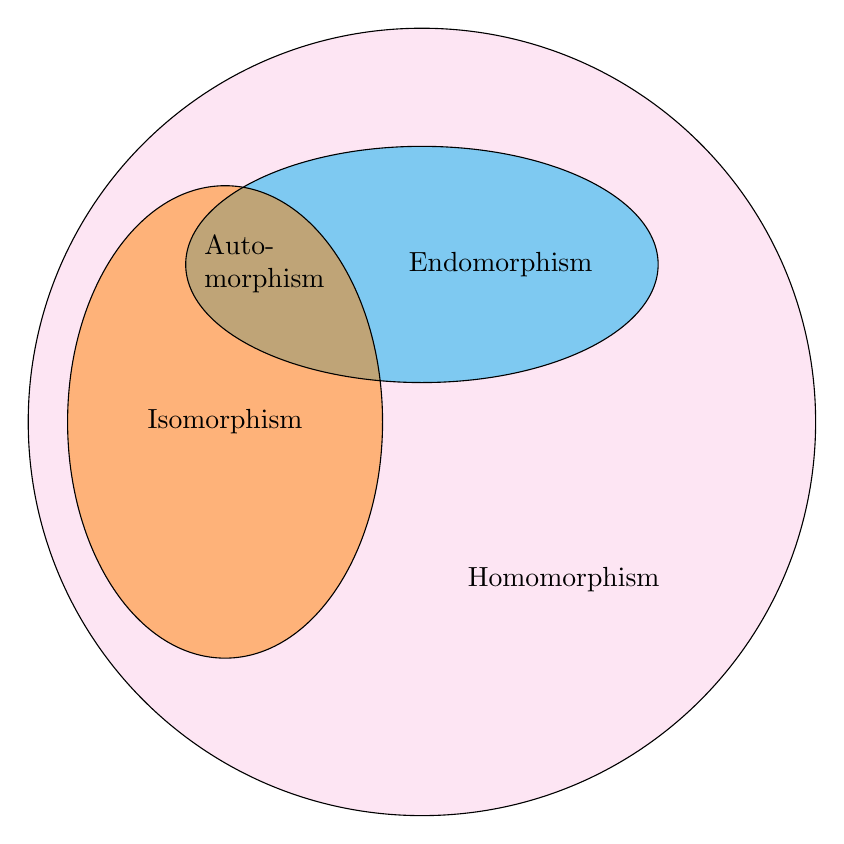
\begin{tikzpicture}
		\def\homomorphism{(0:0cm) circle (5.0cm)}
	  	\def\isomorphism{(180:2.5cm) ellipse (2.0cm and 3.0cm)}
	  	\def\endomorphism{(90:2.0cm) ellipse (3.0cm and 1.5cm)}
	      \begin{scope}[fill opacity=0.1]
	        \fill[magenta] \homomorphism;
	      \end{scope}
	
	      \begin{scope}[fill opacity=0.5]
	        \fill[cyan] \endomorphism;
	      \end{scope}
	
	      \begin{scope}[fill opacity=0.5]
	        \fill[orange] \isomorphism;
	      \end{scope}
	
	      \draw \homomorphism;
	      \draw \isomorphism;
	      \draw \endomorphism;
	
	      {
	        \scalefont{2.0}
	        \node[text=black] at ( 1.8,-2) {Homomorphism};
	      }
	
	      {
	        \scalefont{1.6}
	        \node[text=black] at (-2.5, 0) {Isomorphism};
	      }
	
	      {
	        \scalefont{1.4}
	        \node[text=black] at (   1, 2) {Endomorphism};
	      }
	      \node[align=left] at (  -2, 2) {Auto-\\morphism};
	    \end{tikzpicture}
		\caption[Venn diagram of different types of homomorphisms]{Venn diagram of different types of homomorphisms (source: Wikipedia, author: Martin Thoma}
	\end{figure}
	
	
	\subsubsection{Ideal}
	\textbf{Definition (\#\mydef):} 
	Let $A$ be a commutative ring (like $(\mathbb{R},+,\cdot)$ for example). A subset $S\subset A$ is an "\NewTerm{ideal}\index{ideal}" if:
	\begin{enumerate}
		\item[P1.] For all $a,a'\in S$:
		
	
		\item[P2.] For all $a\in S$ and all $r\in A$:
		
	\end{enumerate}
	In other words, an ideal is a closed subset for addition and stable for the multiplication by any element of $A$.
	\begin{tcolorbox}[colframe=black,colback=white,sharp corners]
	\textbf{{\Large \ding{45}}Example:}\\\\
	The set of even numbers $\mathbb{Z}_{2k}$ is an example of ideal of the set of relative integers $\mathbb{Z}$.
	\end{tcolorbox}
	\begin{tcolorbox}[title=Remark,colframe=black,arc=10pt]
	The ideals $S=\{0\}$ and $S=A$ are named the "\NewTerm{trivial ideals}".
	\end{tcolorbox}
	\begin{dem}
	This results from the property P2 of the definition of an ideal:
	
	For any $r\in A$, we have $r=r\cdot 1\in 1$ because $1\in I$.
	\begin{flushright}
		$\square$  Q.E.D.
	\end{flushright}
	\end{dem}
	Another quite general example of ideal is given by the kernel of a homomorphism of rings. Indeed, let us prove that the kernel of a homomorphism $F:R\mapsto S$ is an ideal of $R$.
	\begin{dem}
	Given $a,a'\in \ker (f)$. Then:
	
	which shows that $a+a'\in \ker(f)$. Given $r\in R$, then:
	
	Which shows that $r\cdot a\in \ker(f)$.
	\begin{flushright}
		$\square$  Q.E.D.
	\end{flushright}
	\end{dem}
	Proposition: Let $A$ be a ring and let $a\in A$. The subset:
	
	Denoted $(a)$ or $aA$, is an ideal (we will see a concrete example after the next small set of definitions).
	
	\textbf{Definitions (\#\mydef):}
	\begin{enumerate}
		\item[D1.] An ideal $I\neq A$ of a ring $A$ is named a "\NewTerm{principal ideal}" if there exists $a\in A$ such as $I=(a)$.
	
		\item[D2.] A ring of which all the ideals are principal is named "\NewTerm{principal ring}".
	\end{enumerate}
	\begin{tcolorbox}[colframe=black,colback=white,sharp corners]
	\textbf{{\Large \ding{45}}Example:}\\\\
	Let us now show that the ring $\mathbb{Z}$ is principal (because all its ideals are principal).\\
	
	Let $I$ be an ideal of $\mathbb{Z}$ (it is easy to choose one: for example, all multiples of $2$ or $3$, etc.). Let $r\in I$ be the smallest non-zero positive integer of $I$. We will show that $I=r\mathbb{Z}=(r)$.\\
	
	Let $a$ be any element of $I$. The Euclidean division allows us to write:
	
	with $0\ge r' <r$ (as we have already prove it).\\
	
	But as $r'=a-qr$ and that $a,r\in I$, by the definition of an ideal, we have $r'\in I$ (the sum or difference of the elements of an ideal belonging to the ideal). By the choice of $r$ ($r'$ being less than $r$) this implies that $r'=0$ and therefore that $a=rq$.\\
	
	Thus every element of $I$ is a multiple $r$ of $q$:
	
	So for the set of even number (denoted as we we know $2\mathbb{Z}$ or $\mathbb{Z}_{2k}$) we have:
	
	\end{tcolorbox}
	The example above uses only the Euclidean division on $\mathbb{Z}$. We can then generalize this result to the rings which possess a Euclidean division. Thus, for example, the ring $K[X]$ of the polynomials (\SeeChapter{see section Calculus page \pageref{polynomial ring}}) with coefficients in a field $K$ is a principal ring because it has an Euclidean division.

	\begin{theorem}
	The ring $K[X]$ of the polynomials with coefficients in a field $K$ is a principal ring (all its ideal are principal)
	\end{theorem}
	\begin{dem}
	Let $I$ be an ideal of $K[X]$. Let us denote by $d$ the smallest degree that can have a non-zero polynomial of $I$. If $d=0$ then $1\in I$ and therefore $I=1\cdot K[X]=K[X]$. Otherwise, given $a(X)$ a polynomial of degree $d$. If $u(X)\in I$ then one can divide $u(X)$ by $a(X)$. There exists therefore $q(X),r(X)\in K[X]$  such as $\deg(r)<\deg(a)=d$ and:
	
	Therefore $r(X)\in I$ which lead to $r=0$ (otherwise contradiction with the minimality of $d$). Therefore,
	
	 We have just shown that:
	
	\begin{flushright}
		$\square$  Q.E.D.
	\end{flushright}
	\end{dem}
	To come back on $\mathbb{Z}$... we have then proved that the only ideals are those of the form $r\mathbb{Z}$. Moreover if we have $d$ and $r$ which are integers $>1$. Then $r\mathbb{Z}\subset d\mathbb{Z}$ if and only if $d | r$.
	\begin{dem}
	If $d | r$ then there exists $n$ with $r=d\cdot n$. Let $m\cdot a$ be an element of $r\mathbb{Z}$. Therefore:
	
	which shows that $r\mathbb{Z}\subset d\mathbb{Z}$.

	Conversely, if $r\in d\mathbb{Z}$ this implies that $r$ is of the form $d\cdot n$ and this proves that $d$ divides $r$.
	\begin{flushright}
		$\square$  Q.E.D.
	\end{flushright}
	\end{dem}
	\begin{theorem}
	Let us also prove that a ring $R$ is a field if and only if it possesses only the trivial ideals:
	
	\end{theorem}
	\begin{dem}
	Let us show that the condition is necessary: Let $I$ be a non-zero ideal of $R$ (that is so say different of $\{0\}$) and $r\in I$ a non-zero element. By hypothesis (that it is a field), it is invertible, that is to say that there exists $t\in R$ such that:
	
	This implies that $1\in I$ and therefore, by a result obtained earlier above $I=R$.
	
	Conversely, suppose that every ideal $I\neq R$ is the null ideal (that is to say $\{0\}$). Then if $r\in R$ is a non-zero element of $R$, the principal ideal $(r)$ must be equal to $R$. But this implies that $1\in (r)$ and therefore that there exists $x\in R$ with $r\cdot x=1$ which shows that $r$ is invertible. The ring $R$ is therefore a field.
	\begin{flushright}
		$\square$  Q.E.D.
	\end{flushright}
	\end{dem}
	This characterization will enable us to easily demonstrate to quite easily prove that:
	\begin{theorem}
	Any homomorphism starting from a field is injective. That is, if $f:R\mapsto S$ is a homomorphism where R is a field, then $f$ is injective.
	\end{theorem}
	\begin{dem}
	We put together what has been seen so far:
	\begin{itemize}
		\item We have proved earlier above that the kernel $\ker(f)$ of a homomorphism of ring is an ideal. 
	
		\item We have also proved just earlier above that we a set was a field if $\{0\}$ and $R$ where the only trivial ideals.
	\end{itemize}
	Therefore for the both point above we have either $\ker(f)=0$ or $\ker(f)=R$ for the field (as it encompass the concept of ring!).
	
	But since $f(1)=1\neq 0$ (by definition of a homomorphism!) it follows that it remains to us only the choice $\ker(f)=\{0\}$. This implies by a previous theorem (where we have proved long time before that if $\ker(f)=\{0\}$ the homomorphism is injective) that ... $f$ is injective.
	\begin{flushright}
		$\square$  Q.E.D.
	\end{flushright}
	\end{dem}
	Let us now study the homomorphisms whose starting ring is $\mathbb{Z}$. Let $A$ be a ring and $f:\mathbb{Z}\mapsto A$ a homomorphism. By definition of a homomorphism and by its properties, it is necessary that as we have defined long time before that $f(0)=0$ and $f(1)=1$ (among others). But we also still need that:
	
	for any $k\in\mathbb{Z}$. Thus $f$ is completely determined by the information of $f(1)$ and is therefore unique.
	
	Conversely, we show that the application $f:\mathbb{Z}\mapsto A$ defined by:
	
	is a homomorphism of rings. In summary, there exists one and only one homomorphism of $\mathbb{Z}$ in any ring $A$.
	
	\textbf{Definition (\#\mydef):} Given $R$ a ring and $f:\mathbb{Z}\mapsto R$ the unique homomorphism defined just previously. If $f$ is injective, we say that $A$ is of "\NewTerm{zero characteristic}\index{zero characteristic}" and we denote it:
	
	Otherwise, $\ker(f)$ is a non trivial ideal of $\mathbb{Z}$ and as $\mathbb{Z}$ is therefore principal (as we have demonstrated above) it is of the form $k\mathbb{Z}$ with $k>0$. The integer $k$ is named the "\NewTerm{characteristic of $A$}\index{characteristic}" and we have therefore:
	
	The definition above may not be very clear (at least for me it is not!). So let us see another approach to introduce the characteristic much more detailed...:
	
	Given $R$ a ring and any of its elements $r$, let us denote integers with boldface type. So $\pmb{1}$ is the integer number one, for instance, $\pmb{0}$ is the integer zero, whereas $0_R$ and $1_R$ are the neutral elements in $R$.

	Since $R$ under addition is an abelian group, we can as usual define:
	
	By definition of a homomorphism, we have if $f:\mathbb{Z}\mapsto R$ that:
	
	then for recall:
	\begin{itemize}
		\item $f(\pmb{m}+\pmb{n})=f(\pmb{m})+f(\pmb{n})$
		\item $f(\pmb{mn})=f(\pmb{m})f(\pmb{n})$
		\item $f(\pmb{1})=1_R$
	\end{itemize}
	so $f$ is a homomorphism of rings. Like all ring homomorphisms, $f:\mathbb{Z}\mapsto R$ has a kernel which is an ideal as we have proved just earlier, so we have $\ker(f)=\pmb{k}\mathbb{Z}$ for a unique $\pmb{k}\ge \pmb{0}$.
	
	If $k=0$, then as we have proved much earlier above, then $f$ is injective. Otherwise, we have:
	
	by definition of the kernel, which means that:
	
	for every $r\in R$. This integer $\pmb{k}$ is the "characteristic" of $S$.
	
	That is, $\text{char}(R)$ is the smallest positive number $\pmb{k}$ such that:
	
	if such a number $\pmb{k}\in\mathbb{N}$ exists, and $0$ otherwise.
	
	\begin{tcolorbox}[colframe=black,colback=white,sharp corners]
	\textbf{{\Large \ding{45}}Example:}\\\\
	E1. The only ring that has $\text{char}(R)=1$ such that:
	
	is the trivial ring $R=\{0_R\}$.\\
	
	E2. The ring $\mathbb{Z}$ is of zero characteristic because the unique homomorphism $f:\mathbb{Z}\mapsto \mathbb{Z}$ is the identity. It is therefore injective.\\
	
	E3. The injections $\mathbb{Z}\mapsto \mathbb{Q}$ and $\mathbb{Z}\mapsto \mathbb{R}$ show that $\mathbb{Q}$ and $\mathbb{R}$ (and also $\mathbb{C}$) are fields of zero characteristic.
	\end{tcolorbox}
	\begin{theorem}
	We now propose to prove that the characteristic of an integral ring (and in particular of a field) is equal to $0$ or to a prime number $p$.
	\end{theorem}
	\begin{dem}
	We show the contraposition. Let $R$ be a ring of characteristic $m\neq$ with $m$ not prime.
	
	There are then natural $n,r\in\mathbb{N}$ constraint by $n,r<m$ such that $m=n\cdot r$.

	Given $f:\mathbb{Z}\mapsto A$ the unique homomorphism (defined earlier above). By definition of $m$ we have then $f(m)=0_A$ but... (!) $f(r)\neq 0 \neq f(n)$. But then (and this it the trick of the proof!):
	
	which shows that $A$ is not integral.
	\begin{flushright}
		$\square$  Q.E.D.
	\end{flushright}
	\end{dem}
	\begin{tcolorbox}[title=Remark,colframe=black,arc=10pt]
	The reciprocal of the theorem is not true as shown in the example of the ring $\mathbb{R}\times\mathbb{R}$ where addition and multiplication are made component by component. It is a ring of zero characteristic but with divisors of zero:
	
	\end{tcolorbox}	
	
	
	\begin{flushright}
	\begin{tabular}{l c}
	\circled{95} & \pbox{20cm}{\score{4}{5} \\ {\tiny 16 votes, 62.5\%}} 
	\end{tabular} 
	\end{flushright}

	%to make section start on odd page
	\newpage
	\thispagestyle{empty}
	\mbox{}
	\section{Probabilities}\label{probabilities}
	\lettrine[lines=4]{\color{BrickRed}P}robability is the measure of the likelihood that an event will occur and therefore the calculation of probabilities handles random phenomena (known more aesthetically as "\NewTerm{stochastic processes}\index{stochastic process}" when their are time-dependent), that is to say, phenomena that do not always lead to the same outcome and that can be studied using numbers their implications and occurrences. However, even if these phenomena have variable outcomes, depending on chance, we observe a certain statistical regularity.

Probability is quantified as a number between $0$ and $1$ (where $0$ indicates impossibility and 1$ $indicates certainty). The higher the probability of an event, the more certain we are that the event will occur.

The concepts related to probabilities have been given an axiomatic mathematical formalization in probability theory (see further below), which is used widely in such areas of study as mathematics, statistics, finance, gambling, science (in particular physics), artificial intelligence/machine learning, computer science, game theory, and philosophy to, for example, draw inferences about the expected frequency of events. Probability theory is also used to describe the underlying mechanics and regularities of complex systems.

\textbf{Definitions (\#\mydef):} There are several ways to define a probability. Mainly we are talking about:
\begin{itemize}
	\item[D1.] "\NewTerm{Experimental or inductive probability}\index{inductive probability}" which is the probability derived from the whole population.

	\item[D2.] "\NewTerm{Theoretical or deductive probability}\index{deductive probability}" which is the known probability through the study of the underlying phenomenon without experimentation. It is therefore an "a priori" knowledge as opposed to the previous definition that was rather referring to a notion of "a posteriori" probability.
\end{itemize}
As it is not always possible to determine a priori probabilities, we are often asked to perform experiments. We must then be able to pass from the first to the second solution. This passage is supposed to be possible in terms of limit (with a population sample whose size approaches the size of the whole population).

The formal modeling of the probability calculus was invented by A.N: Kolmogorov in a book published in 1933. This model is based on the probability space (U, A, P) that we will define a little further and that we can relate to the theory of measurement (\SeeChapter{see section Measure Theory page \pageref{measure theory}}). However, the probabilities were studied in the scientific point of view by Fermat and Pascal in the mid 17th century.

	\begin{tcolorbox}[title=Remark,colframe=black,arc=10pt]
If you have a teacher or trainer who dare to teach statistics and probabilities with examples based on gambling (cards, dice, match, toss, etc.) dispose it to whom it may concern because it would mean that he has no experience in the field and he will teach you anything and no matter how (examples could normally be based on industry, economy or R\&D, in short: areas daily used in companies but especially not on gambling ...!).
	\end{tcolorbox}	
	
\subsection{Event Universe}

\textbf{Definitions (\#\mydef):}

\begin{itemize}
	\item[D1.] The "\NewTerm{universe of events}\index{universe of events}", or "\NewTerm{universe of observables}\index{universe of observables}", $U$ is the set of all possible outcomes (results), named "elementary events" that occur during a random determined test. The universe can be finite (countable) if the elementary events are finite or continuous (uncountable) if they are infinite.

	\item[D2.] Any "\NewTerm{event}\index{event}" $A$ is a set of elementary events and is part of the universe of possible $U$. It is possible that an event is composed of only a single elementary event.
\end{itemize}

	\begin{tcolorbox}[colframe=black,colback=white,sharp corners]
	\textbf{{\Large \ding{45}}Example:}\\\\
	In $(\mathbb{N},+)$ every element is regular and $(\mathbb{N},\times)$ any non-zero element is regular.
	\end{tcolorbox}
	
\begin{itemize}
	\item[D3.] Let $U$ be a universe and $A$ an event, we say that the event $A$ "occurs" (or "is realized") if during the run of the trial the issue $i\:\left( i \in U \right)$ occurs and that $i \in A$ . Otherwise, we say that $A$ "was not realized".

	\item[D4.] The empty subset $\varnothing$ of $U$ is named "\NewTerm{impossible event}\index{impossible event}". Indeed, if during a trial where the event $i$ occurs, we always have $i \in \varnothing$ and the event $\varnothing$ then never occurred.\\\\
If $U$ is finite, or countably infinite, any subset of $U$ is an event, that is no longer true if $U$ is uncountable (we will see in the chapter Statistics why).

	\item[D5.] The set $U$ is also named "\NewTerm{certain event}\index{certain event}". Indeed, if at the end of the trial the event $i$ occurs, we have always (since $U$ is the universe of events). The event $U$ then always occurred.

	\item[D6.] Let $A$ and $B$ be two subsets of $U$. We know that the events $A \cup B$ and $A \cap B$ are both subsets of $U$ then, events that are respectively "\NewTerm{joint events}\index{joint events}" and "\NewTerm{disjoint events}\index{disjoint events}\label{disjoint events}".
	
	\item[D7.] If two events $A$ and $B$ are such that:
	
	the two events may not be feasible during the same trial, then we say that they are "\NewTerm{mutually exclusive events}\index{mutually exclusive events}".

	\item[D8.] If two events $A$ and $B$ are such that:
	
	the two events may be feasible during the same trial (the possibility to see a black cat when we pass under a ladder, for example), we say conversely that they are "\NewTerm{independent events}\index{independent events}".
	
	\item[D9.] "\NewTerm{Randomness}\index{random}" is the lack of pattern or predictability in events. A random sequence of events, symbols or steps has no order and does not follow an intelligible pattern or combination. Individual random events are by definition unpredictable, but in many cases the frequency of different outcomes over a large number of events (or "trials") is predictable.
	
	\begin{tcolorbox}[title=Remark,colframe=black,arc=10pt]
	If we randomly (i.e. uniformly) choose a real number in the interval $[0,1]$ then for every number there is a zero probability that we will pick this number. This does not mean that we did not pick any number at all!\\

	Similarly with the rationals, while infinite, and dense and all that, they are very very sparse in the aspect of measure and probability. It is perfectly possible that if we throw countably many darts at the real line we will hit exactly all the rationals and every rational exactly once. This scenario is highly unlikely, because the rational numbers is a measure zero set.\\

	Probability deals with \textit{what are the odds of that happening}? \underline{a priori}, not a posteriori!! So we are interested in measuring a certain structure a set has, in modern aspects of probability and measure, the rationals have size zero and this means zero probability.\\
	
	More formally, as we will see in the section Statistics page \pageref{probability density function}, the probabilities are obtained by integrating a probability density function $f(x)$ over an interval. The function is non negative and it has the property:
	
	The probability of selecting a real in an interval $[a,b]\subset \mathbb{R}$ is then given by:
	
	The reader can see now that, given a real number $x_0\in\mathbb{R}$, we have:
		
	\end{tcolorbox}	
\end{itemize}

	\pagebreak
	\subsubsection{Infinite monkey theorem}
	The infinite monkey theorem states that a monkey hitting keys at random on a typewriter keyboard for an infinite amount of time will almost surely type a given text, such as the complete works of William Shakespeare. In fact the monkey would almost surely type every possible finite text an infinite number of times. However, the probability of a universe full of monkeys typing a complete work such as Shakespeare's Hamlet is so tiny that the chance of it occurring during a period of time hundreds of thousands of orders of magnitude longer than the age of the universe is extremely low (but technically not zero).
	
	In this context, "almost surely" is a mathematical term with a precise meaning, and the "monkey" is not an actual monkey, but a metaphor for an abstract device that produces an endless random sequence of letters and symbols.
	\begin{theorem}
	If we have an infinite number of monkeys each hitting keys at random on typewriter keyboards then, with probability $1$, one of them will type the complete works of William Shakespeare (something like a randomness machine, which is typing keys randomly at a typewriter, would eventually write any book that's ever existed, given enough time).
	\end{theorem}

	\begin{dem}
	Let $A_n$ be the event that the $n$th monkey types the complete works of Shakespeare. Then if there are $m$ characters on the keyboard and $N$ characters in the complete works of Shakespeare:
	
	for each $n$. Furthermore the $A_n$ are mutually independent (disjoint event). Hence:
	
	Infinitely many of the events $A_n$ occur i.e. infinitely many monkeys will type the complete works of Shakespeare.
	\begin{flushright}
		$\square$  Q.E.D.
	\end{flushright}
	\end{dem}
	 Therefore if we accept infinity in an argument, then we can end up also accepting that "given infinity, anything can happen".

	\pagebreak
	\subsection{Kolmogorov's Axioms}\label{kolmogorov axioms}
	The probability of an event is somehow responding to the notion of frequency of a random phenomena, in other words, at each event we will attach a real number in the interval $[0,1]$, which measure the probability (chance) of realization. The properties of frequencies we can highlight during various trials allow us to determine the properties of probabilities.
	
	Let $U$ be a universe. We say that we define a probability on the events of $U$ if any event $A$ of $U$ we associate a number or measure $P(A)$, named "\NewTerm{a priori probability of event $A$}\index{a priori probability}" or "\NewTerm{marginal probability of $A$}\index{marginal probability}".
	
	Here are the "\NewTerm{Kolmogorov's axioms}\index{Kolmogorov's axioms}":
	\begin{enumerate}
		\item[A1.] For any event $A$:
		
		Thus, the probability of any event is a real number between 0 and 1 inclusive (this is common human sense...).

		\item[A2.] The probability of the certain event or of the set (sum) of possible events is equal to 1:
		

		\item[A3.] If $A \cap B = \varnothing $ two events are incompatible (disjoint), then:
		
		the probability of the merge ("or") of two mutually incompatibles events (or mutually exclusive) is therefore equal to the sum of their probabilities (law of addition). We then speak of "\NewTerm{disjoint probability}\index{disjoint probability}\label{disjoint probability}".
	
		We understand better that the third axiom requires  $A \cap B = \varnothing$ otherwise the  sum of all probabilities could be greater than 1 (imagine again the set diagram of the two events in your head!).
	\end{enumerate}

	\begin{tcolorbox}[colframe=black,colback=white,sharp corners]
	\textbf{{\Large \ding{45}}Example:}\\\\
	Suppose the typewriter has $50$ keys, and the word to be typed is banana. If the keys are pressed randomly and independently, it means that each key has an equal chance of being pressed. Then, the chance that the first letter typed is 'b' is $1/50$, and the chance that the second letter typed is a is also $1/50$, and so on. Therefore, the chance of the first six letters spelling banana is:
	
	less than one in $15$ billion, but not zero, hence a possible outcome.\\
	
	From the above, the chance of not typing banana in a given block of $6$ letters is $1-(1/50)^6$. Because each block is typed independently, the chance $X_n$ of not typing banana in any of the first $n$ blocks of $6$ letters is:
	
	As $n$ grows, $X_n$ gets smaller. For an $n$ of a million, $X_n$ is roughly $0.9999$, but for an $n$ of $10$ billion $X_n$ is roughly $0.53$ and for an $n$ of $100$ billion it is roughly $0.0017$. As $n$ approaches infinity, the probability $X_n$ approaches zero; that is, by making $n$ large enough, $X_n$ can be made as small as is desired, and the chance of typing banana approaches $100\%$.
	\end{tcolorbox}

We will find an example of this kind of disjoint probability in the chapter of Industrial Engineering when studying F.M.E.A. (Failure Modes and Effects Analysis) for fault analysis systems with a complex structure.

In other words in a more general form if $\left( A_{i} \right)_{i \in \mathbb{N}}$ is a sequence of pairwise disjoint events ($A_{i}$ and $A_{j}$ can not occur at the same time though $i \neq j$) then:	


We then speak of "\NewTerm{$\sigma$-additivity}\index{$\sigma$-additivity}" because if we look more closely at the three axioms above the measure $P$ forms a $\sigma$-algebra (\SeeChapter{see section Measure Theory page \pageref{sigma algebra}}).

At the opposite, if the events are not incompatibles (they can overlap or in other words: they have a joint probability), we then have for probability that at most one of the two takes place:


This means that the probability that at most one of the events $A$ or $B$ occurs is equal to the sum of the probabilities for the realization of $A$ or $B$ occurred, minus the probability that $A$ and $B$ occurred simultaneously (we will show later that this is simply equal to the probability that the two do not occur at the same time!).

	\begin{tcolorbox}[colframe=black,colback=white,sharp corners]
	\textbf{{\Large \ding{45}}Examples:}\\\\
	E1. Consider that in a given area, over $50$ years, the probability of a major earthquake is $5\%$ and on the same period the probability a major flood is $10\%$... We would like to know what is the probability that a nuclear plant meets at most one of two events during the same period if the are not incompatibles. We then calculate the probability that from the above equation that gives $14.5\%$...\\
	
	E2. If we throw a handful of two dice, the probability of getting a double is:
	
	Why ? Because all the possible outcomes at launch give $6^2 = 36$ issues and the number of favorable cases of double $1$, double $2$, ... double $6$ is $6$ and so $P=\frac{6}{6^2}=\frac{6}{36}= \frac{1}{6}$.
	\end{tcolorbox}
	
And thus if they were incompatibles we would have then $A \cap B = \varnothing $ we find again the disjoint probability:


An immediate consequence of the axioms (A2) and (A3) is the relations between the probability of an event $A$ and its complement, noted $\bar{A}$ (or more rarely in accordance with the notation used in the chapter of Proof Theory the complementary may be noted $\neg A$):


Let $U$ be a universe with a finite number of $n$ possible outcomes:


where the events:

are named "\NewTerm{elementary events}\index{elementary events}". When these events have the same probability, we say they are "\NewTerm{equiprobables\index{equiprobables}}". In this case, it is very easy to calculate the probability. Indeed, these events being by definition incompatible with each other at this level of our discussion, we have under the third axiom (A3) of probabilities:


but since:


and that the probability of the right hand are by hypothesis equiprobable, we have:


\textbf{Definition (\#\mydef):}
If $A$ and $B$ are not mutually exclusive but independent, we know that by their compatibility $A \cap B=\varnothing$, that (very important in statistics!):


the probability of the intersection ("and" operator) of two independent events is equal to the product of their probabilities (law of multiplication). We name it "\NewTerm{joint probability}\index{joint probability}\label{joint probability}" (this is the most common case).

\begin{tcolorbox}[colframe=black,colback=white,sharp corners]
\textbf{{\Large \ding{45}}Example:}\\\\
Consider that in a given area, over 50 years, the probability of a major earthquake is 5\% and on the same period the probability a major flood is 10\%... Assume that these two events are not mutually exclusive. In other words that they are compatible. We will be interested to their independence. Thus, we would like to know what is the probability that a nuclear power plants meets the two events at the same time, at any time, during this same period. We then calculate the probability from the above equation that gives 0.05\%...
	\end{tcolorbox}
	
Under a more general form, the events $A_1,A_2,...,A_n$ are independent if the probability of the intersection is the product of the probabilities:


	\begin{tcolorbox}[title=Remark,colframe=black,arc=10pt]
	Be careful to not confuse "independent" and "incompatible"!
	\end{tcolorbox}

	So far to summarize a bit we have:

	\begin{table}[H]
	\begin{center}
		\definecolor{gris}{gray}{0.85}
			\begin{tabular}{|p{7.5cm}|p{7.5cm}|}
				\hline
				\multicolumn{1}{c}{\cellcolor{black!30}\textbf{Type}} & 
  \multicolumn{1}{c}{\cellcolor{black!30}\textbf{Expression}}\\ \hline
				2 incompatibles events (disjoints) & $P(A \cup B)=P(A)+P(B)$ \\ \hline
				2 not incompatibles events (joints) & $P(A \cup B)=P(A)+P(B)-P(A \cap B)$ \\ \hline
				2 not incompatibles but independents events & $P(A \cap B)=P(A) \cdot P(B)$\\ \hline
		\end{tabular}
	\end{center}
	\caption{Classical cases of probabilities}
	\end{table}	

Thanks the above definition, we can show that the probability that either $A$ or $B$ is to take place (e.g. at least one of the two but not both at the same time), is simply equal to... the probability that the two do not does not occur at the same time:


We can also use this definition to determine the probability that only one of two events occurs:


\begin{tcolorbox}[colframe=black,colback=white,sharp corners]
\textbf{{\Large \ding{45}}Example:}\\\\
Consider that in a given area, over 50 years, the probability of a major earthquake is 5\% and on the same period the probability a major flood is 10\%.... We would like to know what is the probability that a nuclear power plant exactly meets one of the both events during the same period, assuming they can not occur at the same time. We then calculate the probability from the above equation and that gives 14\%...
	\end{tcolorbox}

There is a common and important area in the industry where the four following relations are frequently used:



This is the "\NewTerm{tree analysis error}\index{tree analysis error}" or "\NewTerm{probabilistic tree analysis}\index{probabilistic tree analysis}" which is used to analyse the possible reasons for failure of a system of any kind (industrial, administrative or other).

To close this part of the chapter consider the following figure displaying Venn diagrams (\SeeChapter{see section Set Theory \pageref{Venn diagrams}}) for all 16 events (including the impossible event) that can be described in terms of two given events $A$ and $B$. In each case, the event is represented by the red area:

	\begin{figure}[!ht]
		\begin{center}
			\includegraphics{img/arithmetics/venn.eps}
		\end{center}	
		\caption{Possible Venn diagrams for two events}
	\end{figure}

Consider the situation where $A$ represents and earthquake and $B$ represents a major flood and $U$ the universe of all dramatics events for a nuclear power plant. We consider that the two events are independents. Then each of the 16 events can be described as follows, either mathematically or verbally.
\begin{enumerate}
	\item An earthquake can occur or a flood or nothing or the both together or any other event (to resume: any event can occur).
	
	\item $A \cup B$: Any event with an earthquake a flood or the both event together can occur.
	
	\item $A \cup B^c$: Any event with earthquake can occur with or without a flood excepted events with a flood not associated to an earthquake.
	
	\item $A^c \cup B$: Any event with earthquake can occur with or without a flood excepted events with a flood not associated to an earthquake.
	
	\item $A^c \cup B^c$: Any event can occur excepted those associated with an earthquake together with a flood.
	
	\item $A$: Any event with an earthquake can occur (this include the events associating an earthquake and a flood).
	
	\item $B$: Any event with a flood can occur (this include the events associating a flood and an earthquake).
	
	\item $(A \cap B) \cup (A^c \cap B^c)$: Any event can occur excepted those including an earthquake without a flood or those including a flood without an earthquake.
	
	\item $(A \cap B^c) \cup (A^c \cup B)$: Any event including an earthquake without a flood or a flood without an earthquake can occur.
	
	\item $B^c$: Any event excepted those including a flood can occur.
	
	\item $A^c$: Any event excepted those including an earthquake can occur.
			
	\item $A \cap B$: Any events associating an earthquake and a flood together can occur.
	
	\item $A \cap B^c$: Any event with an earthquake and without a flood can occur.
	
	\item $A^c \cap B$: Any event with a flood and without an earthquake can occur.
	
	\item $A^c \cap B^c$: Any event can occur excepted those including an earthquake and/or a flood.
	
	\item $A \cap A^c$ or $B \cap B^c$: Impossible Event.
			
\end{enumerate}

\subsection{Conditional Probabilities}\label{bayesian inference}

What can we infer about the probability of an event $B$ knowing that an event $A$ has occurred, aware that there is a link between $A$ and $B$? In other words, if there is a link between $A$ and $B$, the completion of $A$ has to change our understanding of $B$ and we want to know if it is possible to define the conditional probability of an event (relatively) to another event.

This type of probability is named "\NewTerm{conditional probability}\index{conditional probability}" or "\NewTerm{a posterior probability}\index{a posteriori probability}" of $B$ knowing $A$, and is denoted in the context of the study of conditional probabilities:
	
and often in practice to avoid confusion with a possible division:
	
and we sometimes find in U.S. books the notation:
	
or also:
	
We also have the case:
	
	which is named "\NewTerm{likelihood function of $A$}\index{likelihood function}" or "\NewTerm{a priori probability of $A$ given $B$}\index{a priori probability}".

Historically, the first mathematician to have used the correct notion of conditional probability was Thomas Bayes (1702-1761). This is why we often say "\NewTerm{Bayes}\index{Bayes' probabilities}" or "\NewTerm{Bayesian}\index{Bayesian probabilities}" probabilities as soon as conditional probabilities are involved: "\NewTerm{Bayes formula}\index{Bayes' formula}", "\NewTerm{Bayesian statistics}\index{Bayesian statistics}",etc.

The notion of conditional probability that we will introduce is much less simple than it first appears and the conditionals problems are an inexhaustible source of errors of any kind (there are famous paradoxes on the subject and even expert requires peer review to minimize mistakes).

Let's start with a simple example: Suppose we have two dice. Now imagine that we only launched the first die. We want to know what is the probability that by throwing the second dice, the sum of the two numbers is equal to a given minimum value. Thus, the probability of obtaining the minimum value given the value of the first die is totally different from the probability of obtaining the same minimum value in throwing two dice at the same time. How to calculate this new probability?

Let us now formalize the process! After the launch of the first dice, we have:
	
Under the hypothesis that $B \subset A$ , we feel that $P(B/A)$ must be proportional to $P(B)$, the proportionality constant being determined by the normalization:
	
Now let $B \subset A^c$ ($B$ is included in the complement of $A$ so that the events are mutually exclusive). It is then relatively intuitive .... that under the previous hypothesis of incompatibility we have the conditional probability:
	
This leads us to the following definitions of respectively a posteriori and a priori probabilities:
	
Thus, the fact to know that $A$ has occurred reduces all possible outcomes of the universe $U$ of $B$. From there, only the events of type $A \cap B$ are important. The probability of $A$ given $B$ or vice versa (by symmetry) must be proportional to $P(A \cap B)$!

The coefficient of proportionality is the denominator and it ensures the certain event. Indeed, if two events $A$ and $B$ are independent (think the black cat and the scale for example), then we have:
	
and then we see that $P(B/A)$ is equal to $P(B)$ and therefore the event $A$ adds no information to $B$ and vice versa! So in other words, if $A$ and $B$ are independent, we have:
	
Another fairly intuitive way to see things is to represent the probability measure $P$ as a measure of subsets areas (surface) of $\mathbb{R}^2$.

Indeed, if $A$ and $B$ are two subsets of respective areas $P(A)$ and $P(B)$ then the question of what is the probability that a point in the plane belongs to $B$ knowing that it belongs to $A$ it is quite obvious that the probability is given by answer:
	
We would like to indicate that the definition of conditional probability is often used in the following way:
	
named "\NewTerm{formula of compound probabilities}\index{formula of compound probabilities}\label{compound probabilities}" or "\NewTerm{product rule}\index{product rule}". It is written in many different ways (just a matter of notation convention):
	
	Thus, the a posteriori probability of $B$ knowing $A$ can also be written as:
	
	The way that this formula gives an update of the probability hypothesis, $B$, in light of some body of data, $A$, is named the "\NewTerm{diachronic interpretation}\index{diachronic interpretation}". "Diachronic" meaning that something is hapenning over time, in this case the probability of the hypothesis changes, over time, as we see new data.

	In this interpretation the different terms have a name:
	\begin{itemize}
		\item $P(B)$ is the probability of the hypothesis before we see the data, name as we already know, the "prior probability", or just "prior".

		\item $P(B/A)$ is what we want to compute, the probability of the hypothesis after we see the data, named as we already know, the "posterior".

		\item $P(A/B)$ is the probability of the data under the hypothesis, named the "\NewTerm{likelihood}\index{likelihood}".

		\item $P(A)$ is the probability of the data under my hypothesis, name the "\NewTerm{normalizing constant}".
	\end{itemize}
	\begin{tcolorbox}[colframe=black,colback=white,sharp corners]
\textbf{{\Large \ding{45}}Example:}\\\\
Suppose a disease like meningitis. The probability of having the meningitis will be denoted by $P(M)=0.001$ (arbitrary value for the example) and a sign of this disease like headache will be noted $P(S)=0.1$. We assume known that the a posteriori probability of having a headache if we have meningitis is:
	
The Bayes' theorem then gives the a priori probability of having meningitis if we have a headache!:
	
	\end{tcolorbox}
	We also notice that:
	
	So we can know the probability of the event $A$ knowing the elementary probabilities $P(B_i)$ of its causes and the conditional probabilities of $A$ for each $B_i$:
	
	which is named the "\NewTerm{formula of total probabilities}\index{formula of total probabilities}" or "\NewTerm{total probabilities theorem}\index{total probabilities theorem}". But also, for any $j$, we have the following corollary using the previous results that gives us following an event $A$, the probability that it is the cause $B_i$ that produced it:
	
	which is the general form of the "\NewTerm{Bayes formula}\index{Bayes formula}\label{bayes formula}" or "\NewTerm{Bayes' theorem}\index{Bayes' theorem}" that we will use a little in the Statistical Mechanics chapter and through the study of the queueing theory (\SeeChapter{see section Quantitative Management page \pageref{queueing theory}}). You should know that the implications of this theorem are, however, considerable in daily life, in medicine, in industry and in the field of Data Mining.

We often find in the literature many examples of applications of the previous relation with only two possible outcomes $B$ with respect to the event $A$. Therefore we find the Bayes formula written in the following form for each issue:
	
and note that in this particular case (binary outcomes):
	
is an intuitive result.

For binary events, we also have (returning to the theorem of total probabilities seen above):
	

	\begin{tcolorbox}[colframe=black,colback=white,sharp corners]
	\textbf{{\Large \ding{45}}Examples:}\\\\
	E1. A disease affects $10$ people on $10,000$ ($0.1\% = 0.001$). A test has been developed which has a $5\%$ false positives (people not having the disease but for which the test says they are affected) but still always detects the disease if a person has it. What is the probability that a random person for which the test gives a positive result really has this disease?\\\\There is therefore $10,000$ people, $500$ of which are false positives, and we know a posteriori that $10$ people have really the disease. Then the probability that somebody who has a positive test result is really sick is:
	
	This is often a shocking and counter-intuitive result. It also highlights why diagnostic tests must be extremely reliable!\\

	E2. Two machines $M1$ and $M2$ produce respectively 100 and 200 pieces. $M1$ produces $5\%$ defective pieces and $M2$ produces 6\% (posterior probabilities). What is the a priori probability that a defective piece was manufactured by the machine $M1$?\\

	We then have:
	
	E3. From a batch of $10$ pieces with $30\%$ defective, we take a sample of size $3$ without replacement. What is the probability that the second piece is correct (whatever the first is)?\\

	We have:
	
	\end{tcolorbox}
	\begin{tcolorbox}[colframe=black,colback=white,sharp corners]
	E4. We conclude with an important example for companies where employees have more time in their career to pass exams or assessments in the form of multiple choice questions (MCQs). If an employee responds to a question there are two issues: either he knows the answer or he try to guess it. Let $p$ be the probability that the employee know the answer and therefore $1-p$ that he guess it. We admit that the employee who guesses will correctly answer with a probability of $1/m$ where $m$ is the number of proposed answers. What is the a prori probability that an employee (really) knows the answer to a question with $5$ choices if he answered correctly?\\

	Let $B$ and $A$ be respectively the events "the employee knows the answer" and "the employee correctly answers the question". Then the a priori probability that an employee knows (really) the answer to a question that he answered correctly is:
	
	\end{tcolorbox}
	Bayesian analysis provides also a powerful tool to formalize reasoning under uncertainty and the examples we have shown above illustrate how this tool can be difficult to use.
	
	Finally, for a future use in the section of Theoretical Computing, for the Data Mining technique named "binomial naive Bayes classification" we will need a last result!
	
	Let us recall the product rule seen just earlier above:
	
	We can extend this for three variables. Indeed, let us consider:
	
	and let us put $D=B\cap C$ then:
	
	But as the product rule give us also:
	
	Then:
	
	also sometimes denoted:
	
	and in general to $n$ variables:
	
	In general we refer to this as the "\NewTerm{chain rule}\index{chain rule}\label{chain rule}".

	This formula is especially significant for Bayesian Belief Nets . It provides a means of calculating the full joint probability distribution ; in BBNs many of the variables $A_i$ will be conditionally independent which means that the formula can be simplified as shown here .

\subsubsection{Conditional Expectation}\label{conditional expectation}

Now, we will see to the continuous version of the conditional probability by introducing the subject directly with a particular example (the general theory being indigestible) infinitely important in the field of social statistics and quantitative finance. However, this choice (the study of a particular case) implies that the reader has read the first chapter of Statistics to study the functions of continuous distributions and especially that of the Pareto law.

So here's the scenario: Often, in social sciences or economics, we find in the literature dealing with the laws of Pareto statements like the following (but almost never with a detailed proof): whatever your income, the average income of those who have an income above yours is in a constant ratio, greater than $1$, to your income if it follows a Pareto random variable. Then we say that the law is isomorphic to any truncated part itself.

Let $X$ be a random variable equal to the income and following a Pareto with the density (\SeeChapter{see section Statistics page \pageref{pareto distribution}}):

Let's see what it is exactly:

with $k>1,x_m>0,x \geq x_m$ and that has for distribution function (see also the Statistics chapter for the detailed proof):

The sentence begins with "whatever your income ...", then select any income $x_0 \geq x_m$.

Now we need to compute "the average income of those with income higher than $x_0$". It is therefore asked to calculate the expected (average income) of a new random variable $Y$ that is equal to $X$, but restricted to the population of people with an income above $x_0$:

The distribution function of $Y$ is given by:

This expression is of course equal to zero if $x \leq x_0$.
Well, so far we have only do vocabulary. First recall the following conditional probability relation already seen before:

for $x \geq x_0 $ we have for the conditional law:

Before going further, you should be aware that the numerator and denominator are independent but that the whole must be considered, however, as the realization of a single random variable which we denote $Y$. Furthermore, only the numerator is a dependent variable. The denominator can it be considered as a normalization constant.

So we see that the density of $Y$ is given by the function:
	\begin{gather*}
	f_Y(y) = \begin{cases}
	\qquad 0 & y<x_0 \\
	\dfrac{f(y)}{P(X \geq x_0)} & y \geq x_0 \\
	\end{cases}\\
	\end{gather*}
	Now we can calculate the expectation of $Y$:
	
Knowing that (\SeeChapter{see section Statistics page \pageref{pareto tail distribution}}):
	
We finally have:
	
	$\text{E}(Y)$ represents also the average income of those with a income above $x_0$ and as can be seen from the above equality it is in a constant ratio, greater than $1$, to your income $x_0$.

	We can check this result by doing a Monte Carlo simulation in a spreadsheet software (it is interesting to mention it to generalize to situations not computable by hand). You just need to simulate the inverse of the distribution function:
	
	in Microsoft Excel 11.8346:

\begin{center}
 \texttt{=(\$B\$7\^{}\$B\$6}/(1-RANDBETWEEN(1,10000)/10000))\^{}(1/\$B\$6)
\end{center}

and then take the average of the values obtained above or equal to a given $X$ (which corresponds to $x_0$) and ensure that we get the good results as proved above!

Obviously, we could also calculate the conditional variance (verbatim the conditional standard deviation). It may come one day...

\subsubsection{Bayesian Networks}

"\NewTerm{Bayesian networks}\index{Bayesian networks}", also named "\NewTerm{Bayesian Belief Nets}\index{Bayesian Belief Nets}" abbreviated BNNs, are simply a graphical representation of a problem of conditional probabilities to better visualize the interaction between the different variables when they begin to be in large numbers.

This is a technique increasingly used in decision aided software (Data Mining), artificial intelligence (A.I.) and also in the analysis and risk management (ISO 31010 norm).

Bayesian networks are by definition directed acyclic graphs (\SeeChapter{see section  Graphs Theory page \pageref{acyclic graph}}), so that an event can not (even indirectly) influence its own probability, with quantitative description of dependencies between events.

These graphs are used for both knowledge representation models and calculating conditional probabilities machines. They are mainly used for diagnosis (medical and industrial), risk analysis (diagnostics failures, faults or accidents), spam detection (Bayesian filter), voice text and image opinions analysis, fraud detection or bad payers as well as data mining (M.K.M.: Mining and Knowledge Management) in general.

	\begin{tcolorbox}[title=Remark,colframe=black,arc=10pt]
Many systems and software based on drawings or on information in existing databases exists to build and analyse Bayesian networks. Paid solutions: SQL Server, Oracle, Hugin. Free solutions (at this date): Tanagra, Microsoft Belief Network MSBNX 1.4.2, RapidMiner. Personally I prefer the simplicity of the small software MSBNX from Microsoft. For information, in 15 years of professional experience as a consultant I have met so far only one company on more than 800 multinationals which used Bayesian networks... (in transportation).
	\end{tcolorbox}

Use a Bayesian network is assimilated to do "\NewTerm{Bayesian inference}\index{Bayesian inference}". Based on observed information, we calculate the probability of possible known data but not observed.

For a given domain (e.g. medical), we describe the causal relations between variables of interest by a graph (we do not need again to specify that it is acyclic). In this graph, the causal relations between variables are not deterministic, but probabilistic. Thus, the observation of a cause or multiple causes does not always implies the effect or effects that depend on it, but only changes the probability of observing them.

The particular interest of Bayesian networks is to consider simultaneously a priori knowledge of experts (in the graph) and experience contained in the data.

Example of 5 variables with relations (directed acyclic graph) and numbering of states/variables:
\begin{figure}[H]
\centering
\includegraphics{img/arithmetics/bayes_network_example.eps}
\caption{Example of Bayesian network (acyclic oriented) with 5 states}
\end{figure}

Obviously, the construction of the causal graph is based primarily on return of experience (REX) and sometimes results on standards or reports of expert committees. In computing science, the causal graph automatically change depending on the content of databases (think at the Amazon book store in real time target advertisements based on your past purchases or at the Genius Apple service). But we can rarely think to all possibilities and there will sometimes hidden states between two known states that have been forgotten and that would have allowed to better modelize the situations.

Suppose in the example above that with the help of a corporate database, we know that in about $100,000$ man-days, we hat in the company $1,000$ accidents (i.e.. $1\%$ of total) and $100$ machines failures (i.e.. $0.01\% $of total). Then we represent it in the traditional form as follows:
\begin{figure}[H]
\centering
\includegraphics{img/arithmetics/bayes_network_departure.eps}
\caption{Directed acyclic Bayesian network with probability of departure}
\end{figure}

where we have the subset $S2, S4, S5$ which is what experts name a "\NewTerm{serial or linear connection}\index{serial or linear connection}", the triplet $S3, S2, S4$ is a named a "\NewTerm{divergent relation}\index{divergent relation}" (if the arrows were reversed for the triplet, we would have a "\NewTerm{converging relation}\index{converging relation}").

Before going further with our example we will make some observations in relation to these three types of relations:

For clarity, we distinguish first "\NewTerm{conditional independence}\index{conditional independence}" and "\NewTerm{conditional dependence}\index{condition dependence}".

We say that events $A$ and $C$ are "\NewTerm{conditionally independent}\index{conditionally independent}" if given an event $B$ the following equality holds:
	
So the term "conditional" implies the presence of $B$ and the fact that $C$ does not influence the probability of the event $A$.

About "\NewTerm{conditional dependence}", this time we can distinguish three types of relations.
\begin{enumerate}
	\item The conditional dependence of the following type is named a "\NewTerm{serial or linear connection}\index{serial or linear connection}" (already mentioned above):
\begin{figure}[H]
\centering
\includegraphics[scale=0.8]{img/arithmetics/linearconnection.eps}
\caption{Serial/linear Bayesian network}
\end{figure}
where $A$, $B$ and $C$ are dependent (in this particular example there are 3 dependent nodes $A$, $B$ and $C$, but in general this dependence relates to all nodes if there were more than 3)

In addition, $A$ and $C$ are conditionally dependent to $B$. But if the variable $B$ is known, $A$ no longer provides any useful information about $C$ (the path of uncertainty is somehow broken) and therefore $A$ and $C$ become conditionally independent. We then have the conditional probability that simplify as follows:
	
	\item The conditional dependence of the following type is named a "\NewTerm{divergent connection}\index{divergent connection}" (as already mentioned above):
\begin{figure}[H]
\centering
\includegraphics{img/arithmetics/divergentlink.eps}
\caption{Divergent Bayesian network}
\end{figure}
In addition, $B$ and $C$ are conditionally dependent on $A$. But if $A$ is known, $B$ does not provide any more information on $C$ (again the path of uncertainty is somehow broken) and therefore $B$ and $C$ become independent. We then have for example if $A$ is known:
	
	\item The conditional dependence of the following type is named a "\NewTerm{convergence connection}\index{convergence connection}" or "\NewTerm{$V$-Structure}\index{$V$-structure}" (as already mentioned above):
\begin{figure}[H]
\centering
\includegraphics{img/arithmetics/vstructure.eps}
\caption{Convergent Bayesian network}
\end{figure}
where this time the parents are independent.

So $B$ and $C$ are independent but become conditionally dependent on $A$. If $A$ is known, then we have:
	
The dependence between parents therefore requires the observation of their common child.
\end{enumerate}

Now to make a concrete example, suppose our database gives us (thanks to quality managers who always inputs the quality issues) that when a machine failure occurred, 99 times out of 100 (99\%) there has been a total production stop (i.e. 1\% of time there was no production stop) and on all stop production 1\% was not due to a machine failure. What we traditionally represent as follows:
\begin{figure}[H]
	\centering
	\includegraphics[scale=0.8]{img/arithmetics/first_level_bayesian_network.jpg}
	\caption{1st level Bayesian network}
\end{figure}
So the "\NewTerm{implicit probability}\index{implicit probability}" that there is a production stop is given by:
	
	This value represents the implicit proportion of productions stop from the 100,000 man-days (so we can give a proportion of rows in the database that represents a production stop regardless of the cause and even without knowing the details of the database)..
	
	It then follows immediately that the implicit probability that there is no production stop is given by:
		
	This is consistent with what gives us the freeware MSBNX 1.4.2:
	\begin{figure}[H]
		\centering
		\includegraphics[scale=0.75]{img/arithmetics/msbnx_beginning.eps}
		\caption{Beginning of the Bayesian network with MSBNX 1.4.2}
	\end{figure}
	Now suppose we observed a production stop. What is the a posteriori probability that it is due to a machine failure? We then have:
		
	We can also check this with the software MSBNX 1.4.2:
	\begin{figure}[H]
		\centering
		\includegraphics[scale=0.75]{img/arithmetics/msbnx_machine_failure_aposteriori_probability.eps}
		\caption{A Posteriori probability of a production stop due to a machine failure in MSBNX 1.4.2}
	\end{figure}
	Now, imagine that our database gives us (always thanks to quality managers who ensured to input quality issues) that 99 times out of 100 (99\%) when there was a production stop, there was an evacuation. However 5\% of evacuations were identified as having nothing to do with a production stop (i.e. 95\% of evacuations are due to fire exercises OR other events):
	\begin{figure}[H]
		\centering
		\includegraphics[scale=0.8]{img/arithmetics/second_level_bayesian_network.jpg}
		\caption{2nd level Bayesian network}
	\end{figure}
	Now to calculate the implicit probability retrospectively (a posteriori) of evacuations compared to machines failures, we saw that when we had a conditional dependence serie, the conditional probability depends only on the direct parent. Thus, we get:
		
	We can also check this with the software MSBNX 1.4.2:
	\begin{figure}[H]
	\centering
	\includegraphics[scale=0.75]{img/arithmetics/msbnx_implicit_probability_evacuation.eps}
	\caption{Implicit probability of an evacuation in MSBNX 1.4.2}
	\end{figure}
	So the implicit probability of evacuation does not actually depend on machine failures.

	Now suppose we have observed an evacuation. We want to know what is the a posteriori probability that it is due to a machine failure! Then we have:
	
	We can also check this with the software MSBNX 1.4.2:
	\begin{figure}[H]
		\centering
		\includegraphics[scale=0.75]{img/arithmetics/msbnx_a_posteriori_probability_evacuation.eps}
		\caption{A Posteriori probability of an evacuation due to a machine failure in MSBNX 1.4.2}
	\end{figure}
	
	Now we study the case with the alarm and again a database allows us to build a table with different probabilities:

	\begin{figure}[H]
		\centering
		\includegraphics[scale=0.75]{img/arithmetics/second_level_bayesian_network_second_branch.jpg}
		\caption{2nd level Bayesian network with second branch}
	\end{figure}

	Now to calculate the implicit probability that there is an alarm, we will have to consider the four possible situations. We then use the theorem of total probability:
	
What a little more rigorously should be written:
	
The numerical application therefore provides for the implied probability of an alarm:
	
	What can be built and check as follows with MSBNX 1.4.2:
\begin{figure}[H]
	\centering
	\includegraphics[scale=0.75]{img/arithmetics/msbnx_implicit_probability.eps}
	\caption{Implicit probability in MSBNX 1.4.2}
\end{figure}

	It may be useful to the reader to know that he can sometimes found in the literature the following notation:
	
	
	\begin{tcolorbox}[title=Remark,colframe=black,arc=10pt]
	In the particular example studied above all event have only two states. But in practice they can have 3, 4 and more states. Therefore probabilities cross-tables quickly become enormous.
	\end{tcolorbox}

	As in the previous case, suppose we know that there was a working accident. We wish then calculate the a priori probability of an alarm. We then have (observe that the probability depends actually only to the state $S2$ state since the state $S1$ is completely known!):
	
	We can also check this with the software MSBNX 1.4.2:
	\begin{figure}[H]
		\centering
		\includegraphics[scale=0.75]{img/arithmetics/msbnx_implicit_probability_alarm.eps}
		\caption{Implicit probability of an alarm in MSBNX 1.4.2}
	\end{figure}
	So, knowing that there was a work accident increases the probability that there is an alarm (we start from a probability of $10.089\%$ to go to a probability of $10.65\%$).

	To complete this example, we would calculate the a posteriori probabilities $P(S2/S3)$ and $P(S1/S3)$. To do this, we must first calculate the a priori probabilities  $P(S3/S2)$ and $P(S3/S1)$ (this last one has been calculated just before).

	We have for the missing value (which can be easily checked as before with MSNBX 1.4.2 software):
	
We then have:
	
We now have everything we need to calculate the a priori probability of $P(S2/S3)$ and $P(S1/S3)$:
	
	So the a priori probability that there is a machine breakdown when we know that there is an alarm is 0.979\% (i.e. 0.021\% that the trigger of the alarm is not a priori due to a machine failure). Respectively there is, a priori, 0.998\% probability that there is a work accident when we know there is an alarm (and then 0.002\% that it is not a priori due to a work accident).

	From the critical point of view, when there is finally an alarm we can not say a lot of things.... This is because, in this case, to the fact that the events of significant interest both have low probability to occur (work accident and machine failure) and that the employees respond quite well at the start of the alarm (otherwise if the a priori probabilities were high it would mean that the behavior of the employees is not good because we can guess - with exasperation - in advance which problem occurs with a good confidence).

	\begin{tcolorbox}[title=Remark,colframe=black,arc=10pt]
	We did not find how to check these last calculations with MSNBX 1.4.2. If someone finds how to do, it would be great to give us the details of the process.
	\end{tcolorbox}	
	
	To conclude, the reader will have noticed that the calculations can quickly become annoying when the graph becomes complex and this explains the use of computer software. Furthermore, in the banking sector that uses for example Bayesian networks for credit risk, the a priori probability can be more complex. For example we might want to know the a priori probability that there is a machine failure knowing that we have an alarm and an accident:
	

\subsection{Martingales}

A martingale in probabilities (there is another one in stochastic processes) is a technique to increase the chances of winning in gambling while respecting the rules of the game. The principle is completely dependent on the type of game we are focusing, but this term is accompanied by an aura of mystery that some players would know efficient secret techniques to cheat with chance. For example, many players (or candidates to play) search THE martingale that will beat the bank in the most common games in casinos (institutions whose profitability relies almost entirely on the difference - however small - between the chances of winning and losing).

Many martingales are the dream of their author, some are actually inapplicable, some could actually give the possibility to cheat a little. Gambling in general are unfair: whatever the shot played, the probability of winning of the casino (or of the State in the case of a lottery) is greater than this of the player. In this type of game, it is not possible to inverse the chances, just to minimize the probability of gambler's ruin.

The most common example is the roulette wheels martingale. It consists to play a single chance to the roulette wheels (red or black, odd or even) to win, for example, a unit in a series of moves by doubling his bet if we lose, and that until we earn. Example: the player bets 1 unit on red, if red comes out, it stops playing and won 1 unit (2 units less gain setting unit), if black comes out, he doubles his betting by 2 units on red and so on until he wins.

\begin{figure}[H]
\centering
\includegraphics{img/arithmetics/casino_roulette.eps}
\caption[]{Casino roulette wheel}
\end{figure}

Having a chance on two to win, he may think he will eventually win, and when he wins, he is necessarily paid for everything he has played more one unit of his initial bet.

This martingale appears to be safe in practice. Note that in theory, to be sure of winning, we should have the opportunity to play an unlimited number of times.... This has major drawbacks:

This martingale is in fact limited by the bets that the player can do because you have to double the bet every time you lose: 2 times the initial bet, then 4, 8, 16 .... if he loses 10 times, he must be able to bet 1024 times its initial investment for the 11th party! Therefore a lot of money for little gain!

The roulette wheels also have a "0" which is neither red nor black. The risk of losing at every shot is is then larger than 1/2...

In addition, to paralyze this strategy, casinos offer table games per set: from 1 to 100.-, from 2 to 200.-, from 5 to 500.-, ... Therefore it is impossible to use this method on a large number of shots, which increases the risk of losing it all.

Blackjack is a game that has winning strategies: several playing techniques, which usually require to memorize the cards, can overturn the chances in favour of the player. The mathematician Edward Thorp has published in 1962 a book that was at the time a real best-seller. But all these methods require long training weeks and are easily detectable by the croupier (sudden changes in the amounts of bets are typical). The casino has then the opportunity to banish from its establishment the players using this playing martingale.

It should be noted that there are enough advanced methods. One of them is based on the less played combinations. In games where the gain depends on the number of winning players (Lotto...), playing the least played combinations maximize gains. This is how some people sell combinations that would be statistically very rarely used by other players.

Based on this reasoning, we can still conclude that a player who would have been able to determine statistically the least played combinations, to maximize its expected payoff, will in fact certainly not be the only player to have achieved this by the analysis of these famous combinations! This means that in theory the numbers the least played are actually overplayed combinations, the best might be to achieve a mix of played numbers and overplayed numbers to play for the ideal combinations Another conclusion to all this is maybe that the best is to play random combinations which ultimately are less likely to be chosen by the players who incorporate a human and harmonious factor in the choice of their numbers.

\subsection{Combinatorial Analysis}\label{combinatorial analysis}

"\NewTerm{Combinatorial analysis}\index{combinatorial analysis}" (counting techniques) is the field of mathematics that deals with the study of all the issues, events or facts (distinguishable or indistinguishable) with their arrangements (combinations) ordered or not according to some given constraints.

\textbf{Definitions (\#\mydef):}
\begin{enumerate}
	\item[D1.] A sequence of objects (events, issues, objects, ...) is said "\NewTerm{ordered}\index{ordered sequence}" if each suite with a particular order of objects is recognized as a particular configuration.
	
	\item[D2.] A sequel is "\NewTerm{unordered}\index{unordered sequence}" if and only if we are interested in the frequency of appearance of objects regardless of their order.
	
	\item[D3.] The objects (of a sequence) are said "\NewTerm{distincts}\index{distincts objects}" if their characteristics can not to be confused with the other objects.
\end{enumerate}

	\begin{tcolorbox}[title=Remark,colframe=black,arc=10pt]
We chose to put combinatorial analysis in this chapter because when we calculate probabilities, we also often need to know what is the probability of finding a combination or arrangement of given events under certain constraints.
	\end{tcolorbox}

Students often have difficulty remembering the difference between a permutation, an arrangement and a combination. Here is a little summary of what we'll see:
	\begin{itemize}
	 	\item \NewTerm{Permutation}\index{permutation}: We take all the objects.

	 	\item \NewTerm{Arrangement}\index{arrangement}: We choose objects from the original set and the order intervenes.

	 	\item \NewTerm{Combination}\index{combinatorial}: Same as for the arrangement, but the order does not intervenes.	
	\end{itemize}

You must not forget that for each result, the reverse will give the probability of falling respectively on a given permutation/arrangement/combination!

We will present and demonstrate below the 6 most common cases from which we can find (usually) all others:

\subsubsection{Simple Arrangements with Repetitions}\label{simple arrangements with repetitions}

\textbf{Definition (\#\mydef):} A "\NewTerm{simple arrangement with repetition}\index{simple arrangement with repetition}" or equivalently a "\NewTerm{random sampling with replacement (RSWR)}\index{random sampling with replacement (RSWR)} is an ordered sequence of length $m$ of $n$ distinct objects not necessarily all different in the sequence (either: with possible repetitions!).

Let $A$ and $B$ be two finite sets of respective cardinal $m, n$ such that there is trivially $m$ ways to choose an object in $A$ (of type $a$) and $n$ ways to choose an object in $B$ (of type $b$).

We saw in the section Set Theory (page \pageref{cardinal}) that if $A$ and $B$ are disjoint, that:
	

We therefore deduce the following properties:
	\begin{enumerate}
		\item[P1.] If an object can not be at the same time of type $a$ and type $b$ and if there is $m$ ways to select an object of type $a$ and $n$ ways to choose an object of type $b$, then the union of objects gives $m+n$ selections (this is typically the result of the SQL UNION queries without filters in corporate Relational Databases Management System).
		\item[P2.] If we can choose an object type of type $a$ in $m$ ways then an object of type $b$ in $n$ ways, then there is according to the Cartesian product of two sets (\SeeChapter{see section Set Theory page \pageref{cartesian product}}):
		
ways to choose a single object of type $a$ then an object of type $b$.
	\end{enumerate}
With the same notation for $m$ and $n$, we can choose for each element of $A$, its single image among the $n$ elements of $B$. So there are $n$ ways to choose the image of the first element of $A$, then also $n$ ways to choose the image of the second element of $A$, ..., and $n$ ways to choose the image of the $m$-th element of $A$ . The total number of consecutive possible applications from $A$ to $B$ is thus equal to the $m$ product of $n$ (thus $m$ times the cartesian product of the cardinality of the set $B$ with itself!). It is usual to write it under the following way (we have indicated the different ways to write his result as it can be found in various textbooks):
	
where $B^A$ is the set of applications from $A$ to $B$. The increase in the number of possibilities is geometric (not "exponential" as it is often wrongly said!).

This result is mathematically similar to the ordered result (an arrangement where the order of elements in the sequence is taken into account) of $m$ trials in a bag containing $n$ different balls with replacement after each trial. In France this result is traditionally named a "\NewTerm{$p$-list}\index{$p$-list}".

	\begin{tcolorbox}[colframe=black,colback=white,sharp corners]
\textbf{{\Large \ding{45}}Examples:}\\\\
E1. How many (ordered) "words" of 7 letters can we form from a separate alphabet of 24 letters (very useful to know the number of trials to find a password for example)? The solution is:
	
E2. How many groups of people will we have in a referendum on 5 subjects and where each can be either accepted or rejected? The solution is (widely used in some Swiss companies):
	
	\end{tcolorbox}
A simple generalization of this result can consist of the following problem statement:

If we have $m$ such objects $k_1,k_2,...,k_m$ as $k_i$ may take $n_i$ different values then the number of possible combinations is:
	
And if $n_1=n_2=...=n_m$ we have equation then we fall back on:
	
	
	\subsubsection{Simple Permutations without Repetitions}
	\textbf{Definition (\#\mydef):} A "\NewTerm{simple permutation without repetitions}\index{simple permutation without repetition}\label{simple permutation without repetitions}" (formerly named "substitution") of $n$ distinct objects is an ordered (different) sequence of these $n$ objects all different by definition in the sequence (without repetition).

	\begin{tcolorbox}[title=Remark,colframe=black,arc=10pt]
	Be careful not to confuse the concept of permutation ($n$ elements between them) and this of arrangement (of $n$ elements among $m$)!
	\end{tcolorbox}	

	The number of permutations of $n$ items can be calculated by induction: there are $n$ places for a first element, $n-1$ for a second element, ..., and there will be only one place for the last remaining element.

	It is therefore trivial that we the number of permutations is given by:
	
	Recall that the product:
	
is named the "\NewTerm{factorial of $n$}\index{factorial}" and we note it $n!$ for $n \in \mathbb{N}$.

There is therefore for $n$ distinguishable elements\label{distinguishable elements}:
	
as possible permutations. This type of calculation can be useful for example in project management (calculation of the number of different ways to get in a production line $n$ different parts ordered from external suppliers).	

\begin{tcolorbox}[colframe=black,colback=white,sharp corners]
\textbf{{\Large \ding{45}}Example:}\\\\
How many (ordered) "words" of 7 different letters without repetition can we create?
	
This result leads us to assimilate it to the ordered results (an arrangement $A_n$ equation in which the order of elements in the sequence is taken into account) of the trial of balls that are all different from a bag containing $n$ distinguishable balls without replacement.
	\end{tcolorbox}

\subsubsection{Simple Permutations with Repetitions}

\textbf{Definition (\#\mydef):} A "\NewTerm{simple permutation with repetition}\index{simple permutation with repetition}" is when we consider the number of ordered permutations (different) of a sequence of $n$ distinct objects not necessarily all different in a given quantity.

	\begin{tcolorbox}[title=Remark,colframe=black,arc=10pt]
Do not confuse this definition with the "simple arrangement with repetition" seen before!
	\end{tcolorbox}	
	
When some elements are not all distinguishable in a sequence of objects (they are repeated in the sequence), then the number of permutations that we can be do are then trivially reduced to a smaller number then if all the elements were all distinguishable.

Consider $n_i$ as the number of objects of the type $i$, with:	
	
then we write:
	
the number of possible permutations (yet unknown) with repetition (one or more elements in a sequence of repetitive elements are not distinguishable by permutation).

If each of the $n_i$ positions occupied by identical elements were occupied by different elements, the number of permutations could then have to be multiplied by each of the $n_i!$ (previous case).
	
then we deduce:
	
If the $n$ objects are all different in the sequence, we then have:
	
and we fall back again on a simple permutation (without repetition) as:
	

	\begin{tcolorbox}[colframe=black,colback=white,sharp corners]
\textbf{{\Large \ding{45}}Example:}\\\\
How many (ordered) "words" can we create with the letters of the word "Mississippi":
	
	\end{tcolorbox}
This result leads us to assimilate it to an ordered result (a permutation $\bar{A}_n$  where the order of elements in the sequence is not taken into account) of the trial of balls that are not all different from a bag containing $k \geq n$ balls with limited replacement for each ball.

\subsubsection{Simple Arrangements without Repetitions}\label{simple arrangements without repetitions}

\textbf{Definition (\#\mydef):} A "\NewTerm{simple arrangement without repetition}\index{simple arrangement without repetition}" or equivalently a "\NewTerm{random sampling without replacement (RSWOR)}\index{random sampling without replacement (RSWOR)} is an ordered sequence of $p$ objects all distinct taken from $n$ distinct objects with $n \geq p$.

We now propose to enumerate the possible arrangements of $n$ objects among $p$ without repetition. We denote $A_n^p$ the number of these arrangements.

It is easy to calculate that $A_n^1=n$ and to check that $A_n^2=n(n-1)$. Indeed, there are $n$ ways to choose the first object and $(n-1)$ ways to choose the second when we already have the first.

To determine a nice expression for $A_n^p$ , we reason by induction. We assume equation known and we deduce that:
	
It comes: 
	
then:
	
whence:
	
This result leads us to assimilate it to the ordered results (an arrangement $A_n^p$ in which the order of elements in the sequence is taken into account) of the trial of $p$ distinct balls from a bag containing n different balls without replacement.


	\begin{tcolorbox}[colframe=black,colback=white,sharp corners]
	\textbf{{\Large \ding{45}}Example:}\\\\
	Consider the 24 letters of the alphabet, how many (ordered) "words" of 7 distinct letters can we create?
	
	\end{tcolorbox}
The reader may have noticed that if $p=n$ we end up with:
	
So we can say that a simple permutation of $n$ elements without repetition is like a simple arrangement without repetition when $n=p$.

\subsubsection{Simple Combinations without Repetitions}\label{simple combinations without repetitions}

\textbf{Definition (\#\mydef):} A "\NewTerm{simple combination without repetitions}\index{simple combination without repetitions}" or "\NewTerm{choice function}\index{choice function}\label{choice function}" is an non-ordered sequence (where the order doesn't interest us!) of $p$ elements all different (not necessarily in the visual sense of the word!) selected from $n$ distinct objects and is by definition denoted $C_p^n$ in this book and named the "\NewTerm{binomial}\index{binomial}" or "\NewTerm{binomial coefficient}\index{binomial coefficient}\label{binomial coefficient}".

If we permute the elements of each simple arrangement of elements $p$ of $n$, we get all simple permutations and we know that there are in a number of $p!$, using the notation convention of this book we then have (contrary to that recommended one by ISO 31-11!):
	
It is a relation often used in gambling but also in the industry trough the hypergeometric distribution (\SeeChapter{see section Industrial Engineering page \pageref{quality control hypergeometric}}).

	A simple way to remember this function is the following trick: Consider we must select $p$ among $n$ independently of the ordery what are the number of possibilities? 
	
	We know that we have $6\cdot 5\cdot 4=120$ to select them all taking into account the order! The calculation we just made is obviously equal to $n!/p!=6!/3!= 6\cdot 5\cdot 4$. But as the order must not be taken into account we must divide the $120$ by the number of ways we can arrange the $3$ people in the group. So we divide $120$ by $3!$ or more generally and logically by $(n-p)!$. Hence the relation above!
	\begin{tcolorbox}[title=Remark,colframe=black,arc=10pt]
	\textbf{R1.} We have necessarily by construction $C_p^n \leq A_n^p$.\\

	\textbf{R2.} Depending on the authors we inverse the index and suffix of $C$ then you must be careful!
	\end{tcolorbox}
This result leads us to assimilate it to the unordered result (an arrangement $C_n^p$ in which the order of elements of the sequence is not taken into account) of the trial of $p$ balls of a bag containing $n$ different balls without replacement.
	\begin{tcolorbox}[colframe=black,colback=white,sharp corners]
	\textbf{{\Large \ding{45}}Examples:}\\\\
	E1. Consider the 24 letters of the alphabet, how many choices do we have to take 7 letters in the 24 without taking into account the trial order?
		
	The same value can be obtained with the function $\texttt{COMBIN( )}$ of Microsoft Excel 11.8346 (English version).\\
	
	E2. In a Design of Experiment (\SeeChapter{see section Industrial Engineering page \pageref{doe}}) we have $2$ factors of $L=3$ levels each and therefore we need $N=9$ runs to completely determine all the interactions. If we consider that we can take a subset of $S=3$ runs, how many combinations of $3$ among the $9$ can we choose if repititions are vorbidden?
	
	We understand therefore why in Design of Experiments it is important to found a trick to choose the best subset (D-optimum designs)
	\end{tcolorbox}
	There is, in relation to the binomial coefficient, another relation very often used in many case studies and also more globally in physics or functional analysis. This is the "\NewTerm{Pascal's Formula}\index{Pascal's Formula}\label{pascal formula}":
	\begin{dem}
		
We also have $p!=p(p-1)!$, then:
	
and because $(n-p)(n-p-1)!=(n-p)!$:
	
Then:
	
	\begin{flushright}
		$\square$  Q.E.D.
	\end{flushright}
	\end{dem}
	
\subsubsection{Simple Combinations with Repetitions}
	
\textbf{Definition (\#\mydef):} A "\NewTerm{simple combination with repetition}\index{simple combination with repetition}" of $p$ elements of $n$ is a collection of $p$ non-ordered elements, not necessarily distinct.

Simple combinations with repetition are very important for the Wald-Wolfowitz statistical test used in economics and biology and that we will study in the Statistics section.

We will introduce this kind of combination directly with an example an ingenious approach that we have thanks to the physicist and 1938 Nobel Prize in Physics: Enrico Fermi.

Consider $\left\lbrace a, b, c, d, e, f\right\rbrace $ a set having a number $n$ of elements equal to 6 and where we draw a number of elements $p$ equal to 8. We would like to calculate the number of combinations with repetition of elements in a starting set of cardinal 6 in a destination set of cardinal 8.

Consider, for example, the following three combinations:
	
where as the order of elements does not occur, we have grouped the elements to facilitate the reading. Now represent all the above elements by the same symbol "0" and separate the groups consisting of a single element by bars (this is the trick Enrico Fermi). Thus, when one or more elements are not included in a combination, we still denote the separation bars (corresponding to the number of missing elements + the separation of group). Thus, the three combinations above can be written as:
	
We see above that in each case, there are eight "0" (logic. ..) but also that there are also always five "$\mid$". The number of combinations with repetitions of six elements of a starting set to the final one of 8 elements is equal to the number of permutations with repetitions of $8+5=13$ elements, so:
	
We also see that in the general case the number of combinations without consideration of repetitions order can also be written:
	
It is traditional to write this:
	
We also see that:
	
Then:
	
That we also sometimes write:
	
	\begin{tcolorbox}[colframe=black,colback=white,sharp corners]
	\textbf{{\Large \ding{45}}Example:}\\\\
	How many different combinations of outcomes can we make by rolling three standard ($6$-sided) dice if the order of the dice does not matter?\\
	
	The answer is:
	
	But if the order matter, then it was simple $6\cdot 6\cdot 6=216$.
	\end{tcolorbox}
	To resume:
	\begin{table}[H]
		\begin{center}
			\definecolor{gris}{gray}{0.85}
				\begin{tabular}{|p{8cm}|p{6cm}|}
					\hline
					\multicolumn{1}{c}{\cellcolor{black!30}\textbf{Type}} & 
	  \multicolumn{1}{c}{\cellcolor{black!30}\textbf{Expression}} \\ \hline
					Simple arrangement with repetitions & \centering\arraybackslash\ $\bar{A}_n^m=n^m$ \\ \hline
					Simple arrangement without repetitions & \centering\arraybackslash\ $A_m^n=\dfrac{n}{(n-m)!}$  \\ \hline
					Simple permutation without repetitions & \centering\arraybackslash\ $A_n=n!$  \\ \hline
					Simple permutation with repetitions & \centering\arraybackslash\ $\bar{A}_n(n_1,n_2,...,n_k)=\dfrac{n!}{n_1!n_2!...n_k!}$  \\ \hline
					Simple combination without repetitions
	(case of the simple arrangement without repetitions where the order is not taken into account) & 		\centering\arraybackslash\ $C_m^n=\begin{pmatrix}n\\p\end{pmatrix}=\dfrac{A_n^m}{m!}=\dfrac{n!}{m!(n-m)!}$  \\ \hline
					Simple combination with repetitions
	(case of the simple permutation with repetition where the order is not taken into account) & \centering\arraybackslash\ $\Gamma_p^n=C_p^{n+p-1}=\dfrac{(n+p-1)!}{(n-1)!p!}$  \\ \hline
			\end{tabular}
		\end{center}
		\caption{Resume of main Combinatorial Analysis cases}
	\end{table}
	We also have that the number of ways in which $m\cdot n$ different items can be divided equally into $m$ groups ($m=2$ in our example) each containing $n$ objects and the order of the groups is important is:
	
	and the number of ways in which $m\cdot n$ different items can be divided equally into $m$ groups, each containing $n$ objects and the order of the grouops is NOT important is:
	
	
	\begin{figure}[H]
	\centering
	\includegraphics[scale=0.75]{img/arithmetics/gaming.eps}
	\end{figure}

\pagebreak
\subsection{Markov Chains}\label{markov chains}

Markov chains are simple but powerful probabilistic and statistical tools but for which the choice of the mathematical presentation can sometimes be a nightmare... We will try here to simplify a maximum the writings to introduce this great tool widely used in businesses to manage supply chain, in queuing theore for call centers or cash desk, in failure theory for preventive maintenance, statistical physics and biological engineering and also in time series analysis and forecasting (and the list goes on and for more details the reader should refer to the relevant chapters available in this book...).

\textbf{Definitions (\#\mydef):}
	\begin{enumerate}
		\item[D1.] We note by $\left\lbrace X(t) \right\rbrace_{t \in T} $  a probabilistic process function of time whose value at any time depends on the outcome of a random experiment. Thus, at each time $t, X(t)$ is a random variable that we name "\NewTerm{stochastic process}\index{stochastic process}" (for more details on financial applications see the chapter Economy).

		\item[D2.] If we consider a discrete time, we then note  "\NewTerm{discrete time stochastic process}\index{discrete time stochastic process}" as $\left\lbrace X_n \right\rbrace_{n \in \mathbb{N}} $.

		\item[D3.] If we further assume that the random variables $X_n$ can take only a discrete set of values we then speak of "\NewTerm{process in discrete time and discrete space}\index{process in discrete time and discrete space}".
	\end{enumerate}
	\textbf{Definition (\#\mydef):} $\left\lbrace X_n \right\rbrace_{n \in \mathbb{N}} $ is a "\NewTerm{Markov chain}\index{Markov chain}" if and only if:
	
	
in other words (it is very easy!) the probability that the chain is in a certain state on the $n$-th step of the process depends only on the state of the process at step $n-1$ and not on any previous steps!

	\begin{tcolorbox}[title=Remark,colframe=black,arc=10pt]
Also in probabilities a stochastic process verifies the Markov property if and only if the conditional probability distribution of future states, given the present moment, depends only on the present state and not even past states as the relation above. A process with this property is also named a "\NewTerm{Markov process}\index{Markov process}".
	\end{tcolorbox}
\textbf{Definition (\#\mydef):} A "\NewTerm{homogeneous Markov chain}\index{homogenous Markove chain}" is a chain such that the probability that it has to go in a certain state at the $n$-th stage is independent of time. In other words, the probability distribution characterizing the next step does not depend on time (of the previous step), at all times the probability distribution of the chain is always the same for characterizing the transition to the current step.

We can then define (reduce) the law of "\NewTerm{probability transition}\index{probability transition}" of a state $i$ to state $j$ by:
	
It is then natural to define the "\NewTerm{transition matrix}\index{transition matrix}\label{transition matrix}" or "\NewTerm{stochastic matrix}\index{stochastic matrix}":
	
as the matrix that contains all possible transition probabilities between states in an oriented graph.

Markov chains can be represented graphically as an oriented graph $G$ (\SeeChapter{see section Graph Theory page \pageref{oriented graph}}) sometimes named "\NewTerm{automate}\index{automate}" having for the top points (states) $i$ and for the edges the oriented couples $(i, j)$. We then associate to each component an oriented arc and a transition probability.

	\begin{tcolorbox}[colframe=black,colback=white,sharp corners]
	\textbf{{\Large \ding{45}}Example:}\\\\
	\begin{figure}[H]
	\centering
	\includegraphics{img/arithmetics/markov_chain.eps}
	\caption{Generic example of a Markov chain}
	\end{figure}
	Thus, in the example of the oriented graph above, the only allowed transitions from the above $4$ states ($4 \times 4$ matrix) are those indicated by the arrows. So that the transition matrix is then simplified to:
	
	\end{tcolorbox}

The reader has seen in the previous example that we have the trivial property (by construction!) that the sum of the terms (probabilities) of a row of the matrix $P$ is always unitary (and therefore the sum of the terms of a column of the transpose of the matrix unit is still equal to the unit too):
	
and that the matrix is positive (meaning that all its terms are non-negative).

	\begin{tcolorbox}[title=Remark,colframe=black,arc=10pt]
Remember that the sum of the probabilities of the columns is always equal to $1$ for the transpose of the stochastic matrix!
	\end{tcolorbox}	

The analysis of transient state (or: random walk) of a Markov chain consist to determine (or to impose!) to the column-matrix (vector) $p(n)$ to be in a given state at $n$-th step of the walk:
	
with the sum of the components that is always equal $1$ (since the sum of the probabilities of being in any of the vertices of the graph at given a time/step must be equal to $100\%$).

We frequently name this column matrix "\NewTerm{stochastic vector}\index{stochastic vector}" or "\NewTerm{probability measure on the vertex $i$}\index{probability measure}".

\begin{theorem}
We want to prove that the total probability of this stochastic vector is always equal to $1$.
\end{theorem}

\begin{dem}
If $p(n)$ is a stochastic vector, then its image:
	
is also a stochastic vector. Effectively, $p_i(n+1) \geq 0$ because:
	
is a sum of positive or zero values. Furthermore, we find:
	
		\begin{flushright}
			$\square$  Q.E.D.
		\end{flushright}
\end{dem}
This probability vector whose components are positive or zero, depends (it's pretty intuitive) on the transition matrix $P$ and the vector of initial probabilities $p(0)$.

Although even if is provable (Perron-Frobenius theorem), the reader may verify by a practical case (computerized or not!) that if we choose any vector state $p(n)$ then there exists for any stochastic matrix $P$ a unique probability vector traditionally noted $\pi$ as:
	
Such a probability measure $\pi$ satisfying the above equation is named an "\NewTerm{invariant measure}\index{invariant measure}" or "\NewTerm{stationary measure}\index{stationary measure}\label{stationary measure}" or "\NewTerm{balanced measure}\index{balance measure}" which represents the equilibrium state of the system. In terms of linear algebra (see section of the same name page \pageref{linear algebra}) for the eigenvalue $1$, is an eigenvector of $P$ (\SeeChapter{see section Linear Algebra page \pageref{eigenvector}}).

We will see a trivial example in the Graph Theory section (page \pageref{adjacency matrix}) which will be redeveloped in detailed as in the section of Game and Decision Theory in the context of pharmaco-economics (page \pageref{markov decision process}) and in the section of Software Engineering (page \pageref{google pagerank algorithm}) when we will study the fundamentals of the Google PageRank algorithm. But also note that the Markov chains are used for example in meteorology (or in the case of computer passwords hacks):
\begin{figure}[H]
\centering
\includegraphics{img/arithmetics/markov_chain_meteo.eps}
\caption{Concrete example of a very simple Markov chain}
\end{figure}
or in medicine, finance, transportation, marketing, etc.

In the field of language analysis, from the frequency analysis of a sequence of words, computers are able to also build Markov chains and therefore propose a more correct semantic during grammatical computerized corrections or in written transcription of oral presentations.

\textbf{Definitions (\#\mydef):}
	\begin{enumerate}
		\item[D1.] A Markov chain is said to be an "\NewTerm{irreducible Markov chain}\index{irreducible Markov chain}" if all states are bound to others (it's the case of the example in the figure above).

		\item[D2.] A Markov chain is said to be an "\NewTerm{absorbing Markov chain}\index{absorbing Markov chain}" if one of the states of the chain absorbs the transitions (so nothing comes out just to say things in a more simple way!).
	\end{enumerate}
	
	\begin{flushright}
	\begin{tabular}{l c}
	\circled{90} & \pbox{20cm}{\score{4}{5} \\ {\tiny 27 votes, 51.11\%}} 
	\end{tabular} 
	\end{flushright}
	
	%to make section start on odd page
	\newpage
	\thispagestyle{empty}
	\mbox{}
	\section{Statistics}\label{statistics}
	\lettrine[lines=4]{\color{BrickRed}S}tatistics is a science that concerns the systematic grouping of facts or recurring events that lend themselves to a numerical or qualitative assessment over time according to a given law. In the industry and the economy in general, statistics is a science that helps in an uncertain environment to make valid inferences.

	You should know that among all areas of mathematics, the one that is used the most widely in business and research centers is Statistics and especially since softwares greatly facilitates the calculations! This is why this section is one of the biggest in this book even if only the basic concepts are presented!

	Note also that Statistics have a very bad reputation at the university because the notations are often confusing and vary greatly from one teacher to another, from one book to another, from one practitioner to another. Strictly speaking, it should comply with the vocabulary and notation of the ISO 3534-1:2006 norm and unfortunately this section was written before the publication of this standard... a certain period of adaptation will be necessary to obtain the full compliance.

	It is perhaps useless to precise that Statistic is widely used in engineering, robotics, theoretical physics, fundamental physics, econometrics, project management and in the industry of process, in the fields of life and non-life insurance, in the actuarial science or in the database analysis (with Microsoft Excel very often ... unfortunately ....) and the list goes on. We will also meet quite often the tools presented here in the chapters of Fluid Mechanics, Thermodynamics, Technical Management, Industrial Engineering and Economy (especially in the last two). The reader can then refer to them to have some concrete practical applications of the most important theoretical elements that will be seen here.

Note also that in addition to a few simple examples on these pages, many other application examples are given on the exercise server of the companion website in the categories Probability and Statistics, Industrial Engineering, Econometrics and Management Techniques.

\textbf{Definition (\#\mydef):} The main purpose of Statistics is to determine the characteristics of a given population from the study of a part of the population, named "\NewTerm{sample}\index{sample}" or "\NewTerm{representative sample}\index{representative sample}". The determination of these characteristics should enable statistics to be a tool for the decision help!

	\begin{tcolorbox}[title=Remark,colframe=black,arc=10pt]
The data processing concerns the "\NewTerm{descriptive statistics}\index{descriptive statistics}" or also named the "\NewTerm{descriptive analytics}\index{descriptive analytics}". The interpretation of data from estimators is named "\NewTerm{statistical inference}" (or "\NewTerm{inferential statistics}\index{inferential statistics}"), and mass data analysis "\NewTerm{statistical frequency}\index{statistical family}" as opposed to Bayesian inference (\SeeChapter{see section Probabilities page \pageref{bayesian inference}}).
	\end{tcolorbox}	

When we observe an event taking into account some given factors, there can happen that a second observation takes place in conditions that seem identical. By repeating these steps several times on different supposedly similar objects, we find that the observed results are statistically distributed around a mean value that is ultimately the most likely possible outcome. In practice, however, we sometimes perform a single measurement and then the goal is determine the value of the error we make by adopting it as average measure. This determination requires knowledge of the type of statistical distribution we are dealing with and that is on what we will focus (among others) to study here (at least the basics!). However, there are several common methodological approaches whe we face the hazard (less common are not mentioned yet):
	\begin{enumerate}
		\item A first is to simply ignore the random elements, for the simple reason that we do not know how to integrate them. We then use the "scenarios method" also named "deterministic simulation". This is typically the tool used by financial managers and non-graduates managers with tools like Microsoft Excel (which includes a scenarios management tool) or MS Project (which includes a tool to manage the deterministic optimistic, pessimistic and expected scenarios).
		\item A second possible approach, when we do not know how to associate probabilities to specific future random events, is game theory (\SeeChapter{see section Game and Decision Theory page \pageref{game and decision theory}}) where semi-empirical criteria of selection are used as the criterion of maximax, minimax, Laplace, Savage, etc.
		\item Finally, when we can link probabilities to random events, whether these probabilities derived from calculations or measurements, whether they are based on experience from previous similar situations as the current situation, we can use descriptive and inferential statistics (contents of this chapter) to obtain usable and relevant information from this mass of acquired datas.
		\item A last approach when we know the relative probabilities from intervening events in response to strategic choices is the use of decision theory (\SeeChapter{see section Game and Decision Theory pages \pageref{extensive representation of a decision} or \pageref{graphical strategy with probabilities}, \pageref{hurwitz criteria}, \pageref{dove hawk game probabilities} and \pageref{markov decision process}}).
	\end{enumerate}
	\begin{tcolorbox}[title=Remarks,colframe=black,arc=10pt]
\textbf{R1.} Without mathematical statistics, a calculation on datas (e.g. an average), is a "\NewTerm{punctual indicator}\index{punctual indicator}". This is mathematical statistics which gives it the status of estimator whose bias, uncertainty and other statistical characteristics are controlled. We generally seek to ensure that the estimator is unbiased, convergent and efficient (we will see during our study of estimators further what is exactly all that stuff).\\

\textbf{R2.} When we communicate a statistic it should be an obligation to specify the confidence interval, the $p$-value and the size of the studied sample (absolute statistics) and its detailed characteristics and make available the sources and data protocol otherwise it has almost no scientific value (we will see all these concepts in detail further below). A common mistake is to communicate in relative values. For example, on a test group of 1,000 women, 5 women will die from breast cancer without screening check, with screening check 4 women will die. Some will say a little to quickly (typically physicians....) that screening checks saves 20\% of women (relative value as one the of five could have been saved...). In fact this is wrong since the absolute benefit of screening is insignificant!\\\\
\textbf{R3.} If you have a teacher or trainer who dares to teach you statistics and probabilities only with examples based on gambling (cards, dice, matches, coins, etc.) dispose or denounce him. Normally examples should be based on the industry, economy or R\&D, i.e. in areas used in daily by businesses!).
	\end{tcolorbox}	
	
	\subsection{Samples}

During the statistical analysis of sets of information, the way to select the sample is as important as how to analyze it.The sample must be representative of the population (we do not necessarily make reference to human populations!). For this, the random sampling is the best way to achieve it.

\textbf{Definitions (\#\mydef):}
\begin{enumerate}
	\item[D1.] The statistician always starts from the observation of a finite number of elements, which we name the "\NewTerm{population}\index{population}". The observed elements, in quantity $n$, are all of the same nature, but this nature can be very different from one population to another.
	\item[D2.] We are in the presence of a "\NewTerm{quantitative character}\index{quantitative character}" when each observed element is explicitly subject to the same measure. To a given quantitative character, we associate a "\NewTerm{quantitative variable}\index{quantitative variable}" continuous or discrete, which summarizes all the possible values that the measure can take (such information being represented by functions like the Gauss-Laplace distribution, the beta distribution, the Poisson distribution, etc.).
	\begin{tcolorbox}[title=Remark,colframe=black,arc=10pt]
We will come back on the concept of "variable" and "distribution" a little further...
	\end{tcolorbox}	
	\item[D3.] We are in the presence of a "\NewTerm{qualitative character}\index{qualitative variable}" when each observed element is explicitly subject to a single connection to a "\NewTerm{modality}\index{modality}" from a set of exclusive modalities (e.g.: man $\mid$ woman) that permits to classify all studied elements in a given certain point of view (such information being represented by bar charts, sector charts, bubble charts, etc.). All modalities of a character can be established a priori before the survey (a list, a nomenclature, a code) or after the survey. A study population can be represented by a mixed character, or set of modalities such as gender, wage range, age, number of children, marital status for example for an individual.
	\item[D4.] A "\NewTerm{random sample}\index{random sample}" is by default (without more precision) a sample in which all individuals in a population have the same chance, or "\NewTerm{equally likely probability}\index{equally likely probability}" (and we emphasize that this probability must be equal), to end up in the sample.
	\item[D5.]  In the opposite in a sample whose elements were not chosen randomly, then we talk about a "\NewTerm{biased sample}\index{biased sample}" (in the opposite case we talk about a "\NewTerm{non-biased sample}\index{non-biases sample}").
	\begin{tcolorbox}[title=Remark,colframe=black,arc=10pt]
A small representative sample is by far preferable to a large biased sample. But when the sample sizes are small, the hazard can a result worst than the biased one...
	\end{tcolorbox}	
\end{enumerate}

	\subsection{Averages}\label{averages}
	
The concept of "\NewTerm{average}\index{average}" or "\NewTerm{central tendency}\index{central tendency}" (financial analysts call it a "measure of location"...) is with the notion of "variable" at the basis of statistics.

This notion seems very familiar to us and we talk a lot about it without asking too many questions. But there are various qualifiers (we emphasize that this are only qualifiers!) to distinguish the way of the resolution of a problem of calculating the average.

Thus, you must be very very careful about the calculations of averages because there is a tendency in business to rush and to systematically use the arithmetic mean without thinking, which can lead to serious errors! A nice example (for an analogy) is that a considerable number of laws require only moderate levels of pollution per year, while for example, smoking one cigarette per day during 365 days does not have the same impact as smoking 365 cigarettes in one day during one year when both have the same average taken over a year ... This is a clear evidence of statistical incompetence of the legislature.

Here is a small sample of common mistakes:

\begin{itemize}
	\item Consider that the arithmetic mean is the value that divides the population into two equal parts (although it is the median that does this).

	\item Consider that the average of the ratios of the type goals/realisations is equal to the ratio of the average of the goals and of the average of the realizations (although it is not the same thing!).

	\item Consider that the average salaries of different subsidiaries, is equal to the global average (while this is true if and only if there is the same number of employees in each subsidiary of the company).

	\item Consider that the average of the average of the rows in a table is always equal to the average of the columns of the same table (although this is true if and only if the cell contents are not empty).

	\item Calculate the arithmetic average growth of the revenue in \% (as the geometric mean must be used).

	\item etc.
\end{itemize}

We will see below different average with examples relative to arithmetic, to the enumeration, to physics, to econometrics, to geometry and sociology. The reader will find other practical examples by browsing the entire book.

\pagebreak
\textbf{Definitions (\#\mydef):} As given $x_i$ real numbers, then we have:
	\begin{enumerate}
		\item[D1.] The "\NewTerm{arithmetic average}\index{arithmetic average}\label{arithmetic average}" or "\NewTerm{sample average}\index{sample average}" (the most commonly known) is defined as the quotient of the sum of $n$ observed $x_i$ values by the total size $n$ of the sample:
			
	and is very often written $\bar{x}$ or $\widehat{\mu}$  and is for any discrete or continuous statistical distribution an unbiased estimator of the mean.

	The arithmetic average represents a statistical measure expressing the magnitude that would have each member of a set of measures if the total must be equal to the product of the arithmetic average by the number of members.

	If some values repeats more than once in the measurements, the arithmetic mean is then often formally noted as following:
	
	and is named "\NewTerm{weighted average}\index{weighted average}\label{weighted mean}". Finally, we could indicate that under this approach, the actual weighted average will be named "\NewTerm{mathematical mean}\index{mathematical mean}" or just "\NewTerm{mean}\index{mean}" in the field of study of probabilities.

	We may as well use the frequencies of occurrence of the observed values named "\NewTerm{classes frequencies}\index{class frequencies}":
	
	So that we get another equivalent definition named the "\NewTerm{weighted average by the classes frequencies}\index{weighted average by the classes frequencies}\label{weighted average by the classes frequencies}":
	
	Before continuing, it's important to know that in the field of statistics it is useful and often necessary to combine measurements/data in class intervals of a given width (see examples below). We often have to make several tries to choose the intervals even if there are semi-empirical formulas for choosing the number of classes when we have $n$ available values. One of these semi-empirical rules used by many practitioners is to retain the smallest integer $k$ of classes such as:
	
	the width of the class interval is then obtained by dividing the range (difference between the maximum and minimum measured value) by $k$. By convention and rigorously... (so rarely respected in the notations), a class interval is closed on the left and open on the right (\SeeChapter{see section Numbers page \pageref{domain of definition}}):
	
	This empirical rule is named the "\NewTerm{Sturges rule}\index{Sturges rule}" and is based on the following reasoning:

	We assume that the values of the binomial coefficient $C_k^i$ gives the number of individuals in an ideal histogram (we let the reader check this simply with a spreadsheet software like Microsoft Excel 11.8346 and the $\texttt{COMBIN(k,i)}$ function) of $k$ intervals for the $i$-th interval. As as $k$ becomes large the histogram looks more and more like a continuous curve named the "Normal curve" or "bell curve" as as we will see later.

	Therefore, based on the binomial theorem (\SeeChapter{see section Calculus page \pageref{binomial theorem}}), we have:
	
Then, for each interval $i$ the practitioner will traditionally take the average between the lower and upper limit for the calculation and multiply it by the corresponding class frequency $f_i$. Therefore, the grouping of class frequencies implies that:
	\begin{enumerate}
		\item The weighted average by the frequencies differs from the arithmetic average.
		\item As the approximation seen above it will be a worst indicator compare to the arithmetic average...
		\item It is very sensitive to the choice of the number of classes, than very bad at this level.
	\end{enumerate}
There are many other empirical rules for the discretization of random variables. For example, the software XLStat offers not less than 10 rules (constant amplitude, Fisher algorithm, $K$-means, 20/80, etc.).

Later, we will see two very important properties of the arithmetic average and of the mean that you will have to understand absolutely (the weighted average of deviations from the average and the average deviations from the average).

	\begin{tcolorbox}[title=Remark,colframe=black,arc=10pt]
The "\NewTerm{mode}\index{mode}", denoted $\mathrm{Mod}$ or simply $M_0$, is defined as the value that appears most often in a set of data. In Microsoft Excel 11.8346, it is important to know that the $\texttt{MODE( )}$ function returns the first value in the order of values having the largest number of occurrences therefore assuming a unimodal distribution.
	\end{tcolorbox}	
		\item[D2.] The "\NewTerm{median}\index{median}" or "\NewTerm{middle value}\index{middle value}", noted $M_e$ is the value that cut the population values into two equal parts. In the case of a continuous statistical distribution $f(x)$ of a random variable $X$, it is the value that represents the value that has 50\% of cumulative probability to occur (we will see further in details the concept of statistical distribution):
		
In the case of a series of ordered values $x_1,x_2,...,x_i,...x_n$, the median is therefore by definition the value such that we have the same number of values that are greater than or equal to it than the number of values that are less or equal to it.
	\begin{tcolorbox}[title=Remarks,colframe=black,arc=10pt]
	\textbf{R1.} The median is mainly used for skewed distributions, because it represent them better than the arithmetic average.\\
	
	\textbf{R2.} The median is in practice often not a single value (at least in the case where $n$ is even). Indeed, between the values corresponding to ranges $\dfrac{n}{2}$ and $\dfrac{n}{2}+1$ there is an infinite number of values to choose which cut the population in half.
	\end{tcolorbox}	
More rigorously:
	\begin{itemize}
		\item If the number of terms is odd, i.e. of the form $2n + 1$, the median of the series is the term of order $n + 1$ (that the terms are all distinct or not!).
		\item If the number of terms is even, i.e. of the form $2n$, the median of the series is half-sum (arithmetic average) of the values of the terms of rank $n$ and $n + 1$ (that the terms are all distinct or not!).	
	\end{itemize}

In any case, by this definition, it follows that there are at least 50\% of the terms of the serie that are smaller than or equal to the median, and at least 50\% of the terms of the serie that are greater than or equal to the median.

For example, consider the table of wages below:

	\begin{table}[H]
	\begin{center}
		\definecolor{gris}{gray}{0.85}
			\begin{tabular}{|c|c|c|c|}
				\hline
				\multicolumn{1}{c}{\cellcolor{black!30}\textbf{Employee N\degre}} & 
\multicolumn{1}{c}{\cellcolor{black!30}\textbf{Wage}} & \multicolumn{1}{c}{\cellcolor{black!30}\textbf{Cumulated Employees}} & \multicolumn{1}{c}{\cellcolor{black!30}\textbf{\%Cumulated Employees}}\\ \hline
		1 & 1,200 & 1 & 6\%\\ \hline
		2 & 1,220 & 2 & 12\%\\ \hline
		3 & 1,250 & 3 & 18\%\\ \hline
		4 & 1,300 & 4 & 24\%\\ \hline
		5 & 1,350 & 5 & 29\%\\ \hline
		6 & 1,450 & 6 & 35\%\\ \hline
		7 & 1,450 & 7 & 41\%\\ \hline
		8 & 1,560 & 8 & 47\%\\ \hline
\multicolumn{1}{|c|}{\cellcolor{green!30}9} & 
\multicolumn{1}{|c|}{\cellcolor{green!30}1,600} & \multicolumn{1}{|c|}{\cellcolor{green!30}9} & \multicolumn{1}{|c|}{\cellcolor{green!30}53\%}\\ \hline	
		10 & 1,800 & 10 & 59\%\\ \hline
		11 & 1,900 & 11 & 65\%\\ \hline
		12 & 2,150 & 12 & 71\%\\ \hline
		13 & 2,310 & 13 & 76\%\\ \hline
		14 & 2,610 & 14 & 82\%\\ \hline
		15 & 3,000 & 15 & 88\%\\ \hline
		16 & 3,400 & 16 & 94\%\\ \hline
		17 & 4,800 & 17 & 100\%\\ \hline
	\end{tabular}
	\end{center}
	\caption{Identification of the median}
	\end{table}	

There is in the table an odd number $2n + 1$ of values. So the median of the series is the term of rank $n + 1$. This is $1,600.-$ (result that give any spreadsheet software). The arithmetic average is in this case about $2,020.-$.

In direct relation with the median it is important to define the following concept to understand the underlying mechanism:

\textbf{Definition (\#\mydef):} Be given a statistical series $x_1,x_2,...,x_i,...,x_n$, we name "\NewTerm{dispersion of absolute differences}\index{disperson of absolute differences}" around $x$ the number $\varepsilon '(x)$ defined by:
	
$\varepsilon '(x)$ is minimum for a value of $x$ closest to a given value $x_i$ in the sense of the absolute error value. The median is the value that achieves this minimum (extremum)! The idea will then be to study the variations of the function to find the position of this extremum.

Indeed, we can write:
	
Then by definition of the $x$ value:
	
What allows us to skip the absolute values is simply the choice of the index $r$ that is taken so that the serie of values in practice can always be split into two parts: all that is less than the element indexed by $r$ and all that is superior to it (i.e.. the median by anticipation...).

$\varepsilon '(x)$ is also a piecewise (discrete) affine function (similar to the equation of a line for fixed fixed values of $r$ and $n$) where we see that by analogy the factor:
	
is the slope of the function and:
	
the $Y$-intercept (ordinates at the origin).

The function is decreasing (negative slope) until $r$ is less than $\dfrac{n}{2}$ and increasing when r is greater than $\dfrac{n}{2}$ (it passes trough an extremum!). Specifically, we distinguish two particularly cases of interest since $n$ is an integer:

	\begin{itemize}
		\item If $n$ is even, we can say that $n=2n'$, then the slope can be written $2(r-n')$ and it is equal to zero if $r=n$ and then, as the result is valid by construction only for $\forall x \in \left[ x_r,x_{r+1}\right] $ then $\varepsilon '(x)$ is constant on $\left[ x_{n'},x_{n'+1}\right]$ and we have an extremum necessarily in the middle of this range (arithmetic average of the two terms).
		\item If $n$ is odd, we can say that $n=2n'+1$ (we cut the series into two equal parts), then the slope can be written $(2r-2n'-1)$ and it is zero if $r=n'+\dfrac{1}{2}$, as the result is only valid for $\forall x \in \left[ x_r,x_{r+1}\right] $ then it is immediate that the middle value is the median $x_{n'+1}$.
	\end{itemize}
We find out the median in both cases. We will also see later how the median is defined for a continuous random variable (the underlying idea is the same).

There is another practical case where the statistician has at its disposal only the values grouped in intervals of statistical classes. The procedure for determining the median is then different:

When we have at our disposal only a values grouped in intervals of statistical classes, the abscissa of the point of the median is generally within a class. To then get a more accurate value of the median, we perform a linear interpolation. This is what we name the "\NewTerm{linear interpolation method of the median}\index{linear interpolation method of the median}".

The median value can be read from the graph or calculated analytically. Indeed, consider the graph of the cumulative probability $F(x)$ in class intervals as below where the bounds of the intervals were connected by straight lines: 
\begin{figure}[H]
\centering
\includegraphics{img/arithmetics/median_linear_interpolation.eps}
\caption{Graphical representation of the estimation of the median by linear interpolation}
\end{figure}
The value of the median $M_e$ is obviously located at the crossroads between the cumulated probability of 50\% (0.5) and the abscissa. Thus, by applying the basics of functional analysis, we have (just by observing that the slope in the interval containing the median is equal in the half-interval to the left and to right adjacent to the median):
	
What we frequently write:
	
Thus the value of the median:
		
Consider the following table that we will see again much later in this chapter:

	\begin{table}[H]
		\centering
		\renewcommand{\arraystretch}{1.2}
		\small
		\begin{tabular}{cccc}\hline
		Price &  Number & Cumulated number & Relative frequencies  \\[-3pt]
of tickets & of tickets & of tickets & of tickets \\ \hline % ne pas enlever les espaces vides entre les lignes!!!
		[0,50[ & 668 & 668 & 0.068 \\

		[50,100[ & 919 & 1,587 & 0.1587 \\

		[100,150[ & 1,498 & 3,085 & 0.3085 \\

		[150,200[ & 1,915 & 5,000 & 0.5000 \\

		[200,250[ & 1,915 & 6,915 & 0.6915\\

		[250,300[ & 1,498 & 8,413 & 0.8413\\

		[300,350[ & 919 & 9,332 & 0.9332 \\

		[350,400[ & 440 & 9,772 & 0.9772 \\

		[400 and + & 228 & 10,000 & 1 \\ \hline
		\end{tabular}
		\caption{Identification of the median and the mode}
	\end{table}
	We see that the "\NewTerm{median class}\index{median class}" is in the range $[150,200]$ because the cumulative value of $0.5$ is there (column at the right of the table) but the median has, using the previously established relation, the precise value of (it is trivial in the particular example of the table above, but we still do the calculation...):
	
and of course we can do the same with any other percentile!

We can also give a definition to determine the modal value if we are only in possession of the frequencies of class intervals. To see that we start with diagram below named "\NewTerm{grouped distribution}\index{grouped distribution}" in frequencies bar:
\begin{figure}[H]
\centering
\includegraphics{img/arithmetics/modal_value_class_interval.eps}
\caption{Graphical representation of the estimation of the modal value with classes intervals}
\end{figure}
Using the Thales relations (\SeeChapter{see section Euclidean Geometry \pageref{thales theorem}}), it comes immediately, noting $M$ the modal value:
	
As in a proportion, we do not change the value of the ratio by adding the numerators and adding the denominators, we get:
	
We then have:
	
With the previous example this gives then:
	
The question that then arises is to the appropriateness of the choice of the mean, mode or median in terms of communication ... (normally we communicate them all three in corporate reports!).

	A good example is that of the labor market where in general, while the average wage and the median wage are quite different, the institutions of state statistics calculate the median than many traditional media then explicitly equate to he concept of "arithmetic average" in their news...

	\begin{tcolorbox}[title=Remark,colframe=black,arc=10pt]
To avoid getting an arithmetic average having little sense, we often calculate a "\NewTerm{trimmed average}\index{trimmed average}", i.e. an arithmetic average calculated after removing outliers in the series (using Grubbs or Dixon Tests).
	\end{tcolorbox}
	The "\NewTerm{quantile}\index{quantile}" generalize the concept of "median" by cutting the distribution in sets of equal parts (of the same cardinality we might say ...) or in other words in regular intervals. We define the "\NewTerm{quartiles}\index{quartiles}", the "\NewTerm{decile}\index{decile}" and "\NewTerm{percentile}\index{percentile}" on the population, ordered in ascending order, that we divide by $4$, $10$ or $100$ parts of the same size.	So we talk about the 90th percentile to indicate the value separating the first $90\%$ of the population and the $10\%$ remaining.
	
	\textbf{Definitions (\#\mydef):} The "\NewTerm{$P$-th percentile}" ($0<P\leq 100$) of a list of $N$ ordered values (sorted from least to greatest) is the smallest value in the list such that no more than $P$ percent of the data is strictly less than the value and at least $P$ percent of the data is less than or equal to that value. This is obtained by first calculating the ordinal rank and then taking the value from the ordered list that corresponds to that rank. The ordinal rank $n$ is calculated using the relation (using the round to nearest lower integer notation):
	

	Note that in Microsoft Excel 11.8346 the functions \texttt{QUARTILE( )}, \texttt{PERCENTILE( )}, \texttt{MEDIAN( )}, \texttt{PERCENTRANK( )} are available and it can be useful that we specify that there are several variants of calculating these percentiles that explains possible variation between the results of different spreadsheet softwares.
	\begin{tcolorbox}[title=Remark,colframe=black,arc=10pt]
	About Microsoft Excel... and it's conditional formatting tool... the spreadsheet user must not confused the option "percentile" that is based on row numbers on the sorted values of interest on that of "percentage" defined for a vector $\vec{X}$ of values by:
	
	\end{tcolorbox}
	This concept is very important in the context of confidence intervals that we will see much further in this section and very useful in the field of quality with the use of "\NewTerm{box plots}\index{box plots}" (also named "\NewTerm{Box \& Whiskers plots"}\index{Box \& Whiskers plots}) to compare ("discriminate" as experts say) quickly two populations of data or more and especially to eliminate outliers (taking as reference the median will just make more sense!).
	
	\begin{figure}[H]
		\centering
		\includegraphics[scale=0.7]{img/arithmetics/box_plots.eps}
		\caption{Box \& Whiskers Plot painfully made with Microsoft Excel 11.8346}
	\end{figure}
	Or more explicitly as it should be in any good statiscal software:
	\begin{figure}[H]
		\centering
		\includegraphics[scale=0.8]{img/arithmetics/box_plot_template.jpg}
		\caption{Box \& Whiskers Plot ideal chart type}
	\end{figure}
	Another very important mental representation of box plots is the following (it can get an idea of the asymmetry of the distribution as is able to do the R software):
	\begin{figure}[H]
		\centering
		\includegraphics{img/arithmetics/median_mode_quartiles_symetric.eps}
	\end{figure}
	\begin{figure}[H]
		\centering
		\includegraphics[scale=0.75]{img/arithmetics/median_mode_quartiles_asymetric.eps}
		\caption{Graphical representation of the mode, median and 1st + 3rd quartile compared to a distribution}
	\end{figure}
The concepts of median, outliers and confidence intervals that have yet been proved and/or just defined are so significant that there exists international standards for their proper use. First let us cite the norm ISO 16269-7:2001 \textit{Median - Estimation and confidence intervals} and also the norm ISO 16269-4:2010 \textit{Detection and treatment of outliers}.

		A beautiful demonstration on how governments can make statistics lie (hopefully now most of them has to give the data to the population for free) is for example the USA Federal Reserve that pointed out the fact a growth in average income since the 2010. But when you have access to the raw data:
		\begin{center}
			\url{https://www.federalreserve.gov/econres/scfindex.htm}
		\end{center}
		and plot the median versus the average with for example Minitab 17 you get:
		\begin{figure}[H]
		\centering
		\includegraphics[scale=0.8]{img/arithmetics/median_vs_average.jpg}
	\end{figure}
		and after some analysis you can point out that the increase in the average is largely due to increases in the highest $10\%$ of incomes. The decline in the median at the same time suggests that typical Americans are in reality not doing as well... Q.E.D!
		
		\item[D3.] By analogy with the median, we define the "\NewTerm{medial}\index{medial}" as the value (in ascending order of values) that shares the (cumulative) sum values into two equal masses (i.e. the total sum divided by two).

		In the case of our wages example, while the median gives the $50\%$ of the salaries being below and above the medial gives how many employees share (and therefore the sharing wage) the first half and how many employees share the second half of the total of the wages costs.

		\begin{table}[H]
		\begin{center}
			\definecolor{gris}{gray}{0.85}
				\begin{tabular}{|c|c|c|c|}
					\hline
					\multicolumn{1}{c}{\cellcolor{black!30}\textbf{Employee N\degre}} & 
	\multicolumn{1}{c}{\cellcolor{black!30}\textbf{Wage}} & \multicolumn{1}{c}{\cellcolor{black!30}\textbf{Cumulated Wages}} & \multicolumn{1}{c}{\cellcolor{black!30}\textbf{\%Cumulated Wages}}\\ \hline
			1 & 1,200 & 1,200 & 3.5\%\\ \hline
			2 & 1,220 & 2,420 & 7\%\\ \hline
			3 & 1,250 & 3,670 & 10.7\%\\ \hline
			4 & 1,300 & 4,970 & 14.5\%\\ \hline
			5 & 1,350 & 6,320 & 18.4\%\\ \hline
			6 & 1,450 & 7,770 & 22.6\%\\ \hline
			7 & 1,450 & 9,220 & 26.8\%\\ \hline
			8 & 1,560 & 10,780 & 31.4\%\\ \hline
			9 & 1,600 & 12,380 & 36.1\%\\ \hline
			10 & 1,800 & 14,180 & 41.3\%\\ \hline
	\multicolumn{1}{|c|}{\cellcolor{green!30}11} & 
	\multicolumn{1}{|c|}{\cellcolor{green!30}1,900} & \multicolumn{1}{|c|}{\cellcolor{green!30}16,080} & \multicolumn{1}{|c|}{\cellcolor{green!30}46.8\%}\\ \hline
	\multicolumn{1}{|c|}{\cellcolor{green!30}12} & 
	\multicolumn{1}{|c|}{\cellcolor{green!30}2,150} & \multicolumn{1}{|c|}{\cellcolor{green!30}18,230} & \multicolumn{1}{|c|}{\cellcolor{green!30}53.1\%}\\ \hline	
			13 & 2,310 & 20,540 & 59.8\%\\ \hline
			14 & 2,610 & 23,140 & 67.4\%\\ \hline
			15 & 3,000 & 26,140 & 76.1\%\\ \hline
			16 & 3,400 & 29,540 & 86\%\\ \hline
			17 & 4,800 & 34,340 & 100\%\\ \hline
		\end{tabular}
		\end{center}
		\caption{Identification of the mediale}
		\end{table}	

		The sum of all wages is equal to $34,340$ and therefore the medial is $17,170$ then the medial is between the employees No. 11 and 12, while the median was $1,600$. We see then that the medial corresponds to $50\%$ of the aggregate. This is a very useful indicator in Pareto or Lorenz analysis (\SeeChapter{see section Quantitative Management page \pageref{pareto analysis}}).
	
		\item[D4.] The "\NewTerm{root mean square}\index{root mean square}" sometimes denoted simply $Q$ which comes from the general relation:
		
	but where we take $m=2$.
		\begin{tcolorbox}[colframe=black,colback=white,sharp corners]
	\textbf{{\Large \ding{45}}Example:}\\\\
	Consider a square of side $a$, and another square of side $b$. The average area of two squares equals one square of side:
		
		\end{tcolorbox}
	In Microsoft Excel 11.8346 you can combine the functions \texttt{SUMSQ( )}, \texttt{COUNT( )} and to quickly calculate the root mean square as following:
	\begin{center}
	\texttt{=(SUMSQ(...)/COUNT(...))\string^(1/COUNT(...))}
	\end{center}
	
	\item[D5.]  The "\NewTerm{harmonic mean}\index{harmonic mean}" sometimes simply denoted $H$ is defined by:
		
		It is little known but is often the result of simple and relevant arguments (typically the equivalent resistance of an electrical circuit with several resistors in parallel). There is a \texttt{HARMEAN( )} function in Microsoft Excel 11.8346 to calculate it.
		\begin{tcolorbox}[colframe=black,colback=white,sharp corners]
		\textbf{{\Large \ding{45}}Example:}\\\\
Consider a distance $d$ travelled in one direction at the speed $v_1$ and in the other  direction (or not) at the speed $v_2$. The arithmetic average speed will be obtained by dividing the total distance $2d$ by the time of the travel:
		
	If we calculate the time it takes when travel $d$ with a speed $v_i$ that is simply the quotient:
		
	The total time is therefore:
		
	If the distance is not the same for the both velocities anyway each velocity remains the same this is why $d$ disappears!
		\end{tcolorbox}
	In other words: We use the harmonic mean when are given to us ratios.
	
		\item[D6.] The "\NewTerm{geometric mean}\index{geometric mean}\label{geometric mean}" sometimes simply denoted $G$ is defined in the general case by:
		
		This average is often forgotten by undergraduate employees but famous it is famous in the field of finance (\SeeChapter{see section Economy page \pageref{geometric mean for finance}}) this is also why there is an \texttt{GEOMEAN( )} function in Microsoft Excel 11.8346 to calculate it.
		
		A geometric mean is often used when comparing different items – finding a single "figure of merit" for these items – when each item has multiple properties that have different numeric ranges. For example, the geometric mean can give a meaningful "average" to compare two companies which are each rated at $0$ to $5$ for their environmental sustainability, and are rated at $0$ to $100$ for their financial viability. If an arithmetic mean were used instead of a geometric mean, the financial viability is given more weight because its numeric range is larger so a small percentage change in the financial rating (e.g. going from $80$ to $90$) makes a much larger difference in the arithmetic mean than a large percentage change in environmental sustainability (e.g. going from $2$ to $5$). The use of a geometric mean "normalizes" the ranges being averaged, so that no range dominates the weighting, and a given percentage change in any of the properties has the same effect on the geometric mean. So, a $20\%$ change in environmental sustainability from $4$ to $4.8$ has the same effect on the geometric mean as a $20\%$ change in financial viability from $60$ to $72$.
		
		\begin{tcolorbox}[title=Remark,colframe=black,arc=10pt]
		In 2010, the geometric mean was introduced to compute the Human Development Index by United Nations Development Programme. Poor performance in any dimension is directly reflected in the geometric mean. That is to say, a low achievement in one dimension is not anymore linearly compensated for by high achievement in another dimension. The geometric mean reduces the level of substitutability between dimensions and at the same time ensures that a $1\%$  decline in index of, say, life expectancy has the same impact on the HDI as a $1\%$ decline in education or income index. Thus, as a basis for comparisons of achievements, this method is also more respectful of the intrinsic differences across the dimensions than a simple average.
		\end{tcolorbox}
		
		Like for the number $0$, it is impossible to calculate the geometric mean with negative numbers. However, there are several work-arounds for this problem, all of which require that the negative values be converted or transformed to a meaningful positive equivalent value. Most often this problem arises when it is desired to calculate the geometric mean of a percent change in a population or a financial return, which includes negative numbers.

		For example, to calculate the geometric mean of the values $+12\%, -8\%, 0\%$ and +$2\%$, instead calculate the geometric mean of their decimal multiplier equivalents of $1.12, 0.92, 1$ and $1.02$, to compute a geometric mean of $1.0125$. Subtracting $1$ from this value gives the geometric mean of $+1.25\%$ as a net rate of growth (or in financial circles is named the "\NewTerm{Compound Annual Growth Rate C.A.G.R.}\index{compound annual growth rate}").
		\begin{tcolorbox}[colframe=black,colback=white,sharp corners]
		\textbf{{\Large \ding{45}}Example:}\\\\
		Suppose that a bank offers an investment opportunity and plans for the first year an interest (this is absurd, but this is an example) with a rate $(X-Y)\%$ but for the second year with an interest rate $(X+Y)\%$. At the same time another bank provides a constant interest rate for two years: $X\%$. We will say a little bit to fast that this is the same... In fact the two investments do not have the same profitability!\\
	
		In the first bank, a capital $C_0$ will give after the first year of interest:
		
		and the second year:
		
		In the other bank we will have after one year:
		
		and after the second year:
		
		and so on...\\
		As you can probably see it the placement will not be identical if $Y\neq 0$! $X\%$ is the not the arithmetic average of $(X-Y)\%$ and $(X+Y)\%$.

		Now if we write:
		
		What is in reality the average value of the global interest rate $r$?
	
		After $2$ years (for example), the capital is multiplied by $r_1 \cdot r_2$. If an average exists it will be denoted by $r$ and the capital will thus be multiplied by $r^2$. Then we have the relation:
		
		This is an example where we therefore see the geometric mean. Forgetting to use of the geometric mean a common mistake in companies where some employees calculate the arithmetic average rate of increase of a reference value.
		\end{tcolorbox}
		\item[D7.] The "\NewTerm{moving average}\index{moving average}\label{moving average}" of order $n$ is defined as:
		
	The moving average is used particularly in economics, where it represents a trend of a series of values, where the number of points is equal to the total number of points of the serie of values less the number that you specify for the period.

	A moving average in finance is calculated from the average of a stock price over a given period: each point of a moving average of 100 sessions is the average of 100 last current values. This curve, displayed simultaneously with the evolution of the curve of the values, smooths the daily changes in the value and gives the possibility to better see the trends.

	The moving averages can be calculated for different time periods, which can generate short-term trends MMC (20 sessions according to the habits of the domain), medium (50-100 sessions) or long-term MML (over 100 sessions):

	\begin{figure}[H]
		\centering
		\includegraphics[scale=0.75]{img/analysis/time_serie.eps}
		\caption{Graphical representation of a few moving averages}
	\end{figure}

	The crosses of the moving averages with the price curve (cutted with a certain granularity) of the value generate purchase or sale (basic) signals depending on the case:
	\begin{itemize}
		\item Buy signal: when the price curve crosses the MM up.
		\item Sell signal: when the price curve crosses the MM down.
	\end{itemize}
	In addition to the moving average, note that there are a lot of other artificial indicators often used in finance (the R software has a package dedicated only to such indicators). As for example the "\NewTerm{upside/downside ratio}\index{upside/downside ratio}".

The idea is the following: If you have a financial product (\SeeChapter{see section Economy  page \pageref{marketable assets}}) whose current price is $P_c$ for which you have a goal of high gain corresponding to a high price, which we will denote by $P_h$ (high price) and conversely, the potential loss that you feel is at a price $P_l$ (low price).
	

	\begin{tcolorbox}[colframe=black,colback=white,sharp corners]
	\textbf{{\Large \ding{45}}Examples:}\\\\
	E1. For example, a financial product of $10.-$ with a low price of $5.-$ and a high price of $15.-$ has a ratio of $\text{UD}_R=1$ and therefore an identical speculative factor to allow a gain or loss of $5.-$.\\
	
	E2. A financial product of $10.-$ with a low price of $5.-$ and a high price of $20.-$ has a ratio of $\text{UD}_R=2$ and therefore twice the speculative potential gain compared to the loss.
	\end{tcolorbox}
	\begin{tcolorbox}[title=Remark,colframe=black,arc=10pt]
	Some financial institutions recommend to refuse equation below $3$. Investors also tend to reject too high equation that can be a sign of artificial inflation.
	\end{tcolorbox}	
		\item[D8.] The "\NewTerm{weighted average}\index{weighted average}" (the moving average and arithmetic average are just a special cases of the weighted average with $w_i=1$) is defined by:
		
Is used for example in geometry to locate the centroid of a polygon, in physics to determine the center of gravity or in statistics to calculate the mean and other advanced regression techniques and in project management for estimating task durations forecast.

In the general case the weights $w_i$ represents the weighted influence or arbitrary/empirical influence of the element $x_i$ relatively to the others one.
		\item[D9.] The "\NewTerm{functional mean}\index{functional mean}" or "\NewTerm{integral average}\index{integral average}\label{integral average}" is defined as:
		
where $\mu_f$ depends of a function $f$ of a real integrated variable (\SeeChapter{see Differential and Integral Calculus}) on a range $[a, b]$. It is often used in signal theory (electronics, electrotechnichs).
	\end{enumerate}
	
	\pagebreak
	\subsubsection{Laplace Smoothing}

To come back to our class frequencies seen above and before proceeding with the study of some mathematical properties of the averages... you should know that when we work with discrete probabilities distributions it happens very (very) often that we meet a typical problem whose source is the size of the population.

Consider as an example the case where we have $12$ documents and that we would like estimate the probability of occurrence of the word "Viagra". We have on a sample the following values:

	\begin{table}[H]
	\begin{center}
		\definecolor{gris}{gray}{0.85}
			\begin{tabular}{|c|c|}
				\hline
\multicolumn{1}{c}{\cellcolor{black!30}\textbf{Document ID}} & \multicolumn{1}{c}{\cellcolor{black!30}\textbf{Word occurences}} \\ \hline
		1 & 1 \\ \hline
		2 & 0 \\ \hline
		3 & 2 \\ \hline
		4 & 0 \\ \hline
		5 & 4 \\ \hline
		6 & 6 \\ \hline
		7 & 3 \\ \hline
		8 & 0 \\ \hline
		9 & 6 \\ \hline
		10 & 2 \\ \hline	
		11 & 0 \\ \hline
		12 & 1 \\ \hline
	\end{tabular}
	\end{center}
	\caption[]{Class frequencies of the word}
	\end{table}

Table that we can represent in another way:

	\begin{table}[H]
	\begin{center}
		\definecolor{gris}{gray}{0.85}
			\begin{tabular}{|c|c|c|}
				\hline
\multicolumn{1}{c}{\cellcolor{black!30}\textbf{Word occurences}} & \multicolumn{1}{c}{\cellcolor{black!30}\textbf{Documents}} & \multicolumn{1}{c}{\cellcolor{black!30}\textbf{Probability}} \\ \hline
		0 & 4 & 0.33\\ \hline
		1 & 2 & 0.17\\ \hline
		2 & 2 & 0.17\\ \hline
		3 & 1 & 0.083 \\ \hline
		4 & 1 & 0.083\\ \hline
		5 & 0 & 0\\ \hline
		6 & 2 & 0.17\\ \hline
	\end{tabular}
	\end{center}
	\caption[]{Respective frequencies classes of documents}
	\end{table}
	
And here we have a common phenomenon. There is no record with $5$ occurrences of the word of interest. The idea (very common in the field of Data Mining) is then to add artificially and empirically using a count using a technique named "\NewTerm{Laplace smoothing}\index{Laplace smoothing}" which involves adding k units at each occurrence. Therefore the table becomes:

	\begin{table}[H]
	\begin{center}
\begin{tabular}{|c|c|c|}
				\hline
\multicolumn{1}{c}{\cellcolor{black!30}\textbf{Word occurences}} & \multicolumn{1}{c}{\cellcolor{black!30}\textbf{Documents}} & \multicolumn{1}{c}{\cellcolor{black!30}\textbf{Probability}} \\ \hline
		0 & 5 & 0.26\\ \hline
		1 & 3 & 0.16\\ \hline
		2 & 3 & 0.16\\ \hline
		3 & 2 & 0.11 \\ \hline
		4 & 2 & 0.11\\ \hline
		5 & 1 & 0.05\\ \hline
		6 & 3 & 0.16\\ \hline
	\end{tabular}
	\end{center}	
	\caption[]{Frequencies classes of documents with smoothing}
	\end{table}
	
Obviously this type of technique is debatable and beyond the scientific framework ... We even hesitated to introduce this technique in the chapter of Numerical Methods (with the rest of all the empirical numerical techniques) rather than here...

	\subsubsection{Means and Averages properties}\label{means and averages properties}
	
	Now we will see some relevant properties that connect some of these means and averages or are specific to a particular mean/average.

	\label{properties of the mean}The first properties are important so beware to understand them:
	\begin{enumerate}
		\item[P1.] The calculation of the arithmetic, root mean square and harmonic average/mean can be generalized using the following expression:
			
		where we see:
			\begin{enumerate}
				\item For $m=1$, we get the arithmetic average
				\item For $m=2$, we get the root mean square
				\item For $m=-1$ we get the harmonic mean
			\end{enumerate}
		\item[P2.] The arithmetic average has the property of linearity, that is to say (without proof because it is simple to check):
			
			This is the statistical version of the property of the mean in the field of probabilities that we will see further.
			\item[P3.] The weighted sum of the deviations from the arithmetic average is zero.
				\begin{dem}
					First, by definition, we know that:
						
					then we have:
						\thickmuskip=0mu
						\medmuskip=0mu
						
						\thickmuskip=3mu
						\medmuskip=3mu
					Thus, this tool can not be used as a measure of dispersion!

					By extension, the arithmetic average of the weighted deviations from the average is also equal to zero:
					
					\begin{flushright}
						$\square$  Q.E.D.
					\end{flushright}
				\end{dem}
				This result is quite important because it will further be useful for a better understanding of the concept of standard deviation and variance.
			\item[P4.] Now we would like to prove that:
				
					\begin{tcolorbox}[title=Remark,colframe=black,arc=10pt]
The comparisons between the above means/averages and the median or the weighted or moving averages does not make sense this is why we won't compare them.
	\end{tcolorbox}
				\begin{dem}
					First, we consider two nonzero real numbers $x_1$ and $x_2$ as $x_2>x_1>0$ and then we write:
					\begin{enumerate}
						\item The arithmetic average:
							
						\item The geometric mean:
							
						\item The harmonic mean:
							
						\item The root mean square:
										
					\end{enumerate}
					We will start to prove that $\mu_g>\mu_h$ by contradiction by putting $\mu_g-\mu_h<0$:
					
					By convenience we will now put:
						
					and we know that $y>1$. We therefore have:
						
						and remember we search if it is possible that:
						
						 We can now easily check this statement from the following equivalences:
						 
						There is also a contradiction, and this validates our initial hypothesis:
							
						Let see if $\mu_g>\mu_a$.
						
						Under the hypothesis $x_2>x_1>0$. We search now to prove that:
							
						Now we have the following equivalences:
							
						and the last expression is obviously correct because the square of a (real) number is always positive which verifies our initial hypothesis:
							
						We will prove now that $\mu_q > mu_a$ by contradiction by putting $\mu_q-\mu_a<0$:
						
						But the square of a (real) number is always positive which verifies our initial hypothesis:
						
						We then have:
						
						\begin{flushright}
							$\square$  Q.E.D.
						\end{flushright}
				\end{dem}
				Once these inequalities proved, we can then move on to a figure that we attribute to Archimedes to place three of these averages. The interest of this example is to show that there are some remarkable relations between statistics and geometry (coincidence??).
				
				\begin{figure}[H]
					\centering
					\includegraphics[scale=0.75]{img/arithmetics/averages.eps}
					\caption{Starting point for the geometric representation for the various averages}
				\end{figure}
				We will first write $a=\overline{AB},b=\overline{BC}$ and $\text{O}$ is the midpoint of $\overline{AC}$. Thus, the circle is drawn with center $\text{O}$ and radius $\overline{\text{O}A}$. $D$ is the intersection of the perpendicular segment $\overline{AC}$ through $B$ and of the circle $\Omega$ (we can choose the intersection we want). $H$ is itself the orthogonal projection of $B$ on $\overline{OD}$.
				
				Archimedes says that $\overline{\text{O}A}$ is the arithmetic average of $a$ and $b$ and that $\overline{BD}$ is the geometric mean of $a$ and $b$, and $\overline{DH}$ is the harmonic mean of $a$ and $b$.
				
				We then prove that (could be trivial):
					
Therefore $\overline{\text{O}A}$ is the arithmetic average $\mu_a$ of $a$ and $b$.

We have in the right-angled triangle $ADB$:
	
Then we have in the right-angled triangle $BDC$:
	
	We then add these two relations, and we get:
	
	We know that $D$ is on a circle of diameter $\overline{AC}$, so $ADC$ is rectangle on $D$. Therefore:
	
	And then we replace $\overline{BA}$ and $\overline{BC}$ by $a$ and $b$:
		
	So finally:
		
	And therefore, $\overline{DB}$  is the geometric mean $\mu_g$ of $a$ and $b$.
	We have now prove that $\overline{DH}$ is the harmonic mean of $a$ and $b$. We have in a first time using the orthogonal projection as study in the section of Vector Calculus (page \pageref{orthogonal projection vector}):
		
		Then we also have (also orthogonal projection)
		
		Therefore we have:
		
		and since ${DB}=\sqrt{ab}$, we have then:
			
		$\overline{DH}$ is therefore the harmonic mean of $a$ and $b.$ Archimedes was not wrong!
	\end{enumerate} 
	
	\paragraph{Jensen Inequality}\mbox{}\\\\
	The "\NewTerm{Jensen's inequality}\index{Jensen's inequality}\label{jensen inequality}" is a particularly important relation (or property) in finance and insurance because it shows by the proof why an options seller will take the expected mean of pay-off rather than pay-off of the expect mean or why ultimately the insured will always pay more or equal than the differential of the expected mean of accident costs, and also in time series analysis why GARCH processes are naturally leptokurtic and also for the proof the the Kullback-Leibler divergence is strictly positive or null (\SeeChapter{see section Statistical Mechanics page \pageref{kullback-leibler diverence}}).

	\begin{theorem}
	Jensen's inequality will allow us to prove that for a convex function:
	
	with $p_i>0$, $\sum_i p_i=1$. Either by using notations specific to the domain of statistics:
	
	and to the valuation of options (\SeeChapter{see section Economy page \pageref{jensen inequality finance}}):
	
	\end{theorem}
	Before proceeding further, let us recall that a function $f$ is concave if $-f$ is convex and vice versa. It is then immediate that:
	
	Either by using notations specific to the domain of statistics:
	
	Let's go to the proof and then we will make a small practical simplified example with derivatives in finance.
	\begin{dem}
	Let us see if: 
	
	is true by proceeding by induction. First for $m=2$, we fall back on the classical definition (\SeeChapter{see section Functional Analysis page \pageref{convex function}}) of a convex function:
	
	Now, we assume the previous relation true for $m=n$, and we show that it is also true for $m=n+1$:
	
	Since is $f$ is convex, we can write:
	
	Let us put:
	
	for $i=1\ldots n$. We have $q_i>0$ for all $i=1\ldots n$ and:
	
	because for recall:
	
	and consequently:
	
	By hypothesis of recurrence we then have:
	
	And therefore:
	
	by simplifying the expression on the right we get indeed:
	
	\begin{flushright}
		$\square$  Q.E.D.
	\end{flushright}
	\end{dem}
	\begin{tcolorbox}[colframe=black,colback=white,sharp corners]
	\textbf{{\Large \ding{45}}Example:}\\\\
	We know that the pay-offs of a Call and a Put are respectively at maturity (from the point of view of a buyer and therefore by symmetry from the point of view of a seller also in absolute value):
	
	Let us consider a price at maturity of $102$.- and that the possible strikes at maturity are $\{100,110,150\}$, we have then have:
	
	and:
	
	and so we have well for a Call from the point of view of a buyer or seller in absolute values:
	
	\end{tcolorbox}

	\pagebreak
	\subsection{Type of variables}
In talking about variables quantitative or qualitative variables, sometimes you hear variables being described as categorical (or sometimes nominal), or ordinal, or interval.  Below we will define these terms and explain why they are important.

\textbf{Definitions (\#\mydef):}
	\begin{enumerate}
		\item[D1.] The "\NewTerm{discrete variables}\index{discrete variables}" (by counting) that belongs to $\mathbb{Z}$: Are analyzed with statistical laws based on a countable definition domain always strictly positive (the Poisson or Hypergeoemetric distribution are such typical case in the industry). Are almost always represented graphically by histograms.

	\item[D2.] The "\NewTerm{continuous variables}\index{continuous variable}" (by measure) that belong to $\mathbb{R}$: Are analyzed with statistical laws based on an uncountable domain of definition strictly positive or may take any positive or negative value (typically the Normal distribution in the industry). Are almost always represented graphically by histograms with class intervals.

	\item[D3.] The "\NewTerm{attribute variables}\index{attribute variable}" (by classification): They are not digital data (only when they are coded with digits!) but qualitative data type {Yes, No}, {Passed, Failed}, {On time, Late}, {red, green blue, black}, etc. The binary data type attribute follow a Bernoulli while higher order qualitative variables have no average or standard deviation (effectively... try to calculate the mean and standard deviation between the qualitative variables Red, Green and Pink...).
	
	In attribute variable we mainly distinct two subtypes of variables:
		\begin{enumerate}
			\item A "\NewTerm{categorical variable}\index{categorical variable}" (sometimes named a \NewTerm{nominal variable}\index{nominal variable}) is one that has two or more categories, but there is no intrinsic ordering to the categories.  For example, gender is a categorical variable having two categories (male and female) and there is no intrinsic ordering to the categories.  Hair color is also a categorical variable having a number of categories (blonde, brown, brunette, red, etc.) and again, there is no agreed way to order these from highest to lowest.  A purely categorical variable is one that simply allows you to assign categories but you cannot clearly order the variables.  If the variable has a clear ordering, then that variable would be an ordinal variable, as described below.
			\item An "\NewTerm{ordinal variable}\index{ordinal variable}" is similar to a categorical variable.  The difference between the two is that there is a clear ordering of the variables.  For example, suppose you have a variable, economic status, with three categories (low, medium and high).  In addition to being able to classify people into these three categories, you can order the categories as low, medium and high. Now consider a variable like educational experience (with values such as elementary school graduate, high school graduate, some college and college graduate). These also can be ordered as elementary school, high school, some college, and college graduate.
		\end{enumerate}
	\end{enumerate}
	\begin{figure}[H]
		\centering
		\includegraphics[scale=0.75]{img/arithmetics/type_of_variables.jpg}	
		\caption{Type of variables in statistics}
	\end{figure}
	Understanding the different types of data is an important discipline for the engineers because it has important implications for the type of analysis tools and techniques that will be used.

A common question regarding the collection of data is what is the amount that should be collected. In fact it depends on the desired level of accuracy. We will see much further in this section (with proof!) how to mathematically determine the amount of data to collect.

Now that we are relatively familiar with the concept of average (mean), we can discuss on more formal calculations and that will make sense.

	\subsubsection{Discrete Variables and Moments}
	
	Consider $X$ is an independent variable (an individual of a sample, whose property is independent of other individuals) that can take discrete random values (realizations of the vector $(X_1,X_2,...,X_n)$) with respective probabilities $(p_1,p_2,...,p_n)$ where, by the axioms of probabilities (\SeeChapter{see section Probabilities page \pageref{kolmogorov axioms}}):
		
	
	\textbf{Definitions (\#\mydef):}
	\begin{enumerate}
		\item[D1.] Let $X$ be a numeric (quantitative) random variable (r.v.). It will be fully described in practice most of time by the value of the probability (for discrete variables) for a realization of this variable or by the cumulative probability (for discrete AND continuous variables) to be typically less than or equal $X$ for all realizations $x$. This cumulative probability is denoted by:
		
		with:
		
		where $F(x)$ is named the "\NewTerm{repartition function}\index{repartition function}" of the random variable $X$. It is the theoretical proportion of the population whose value is less than or equal to $x$. It follows for example:
		
		More generally, for any two numbers $a$ and $b$ with $a<b$, we have:
		
		
		\item[D2.] The "\NewTerm{empirical repartition function}\index{empirical repartition function}" is naturally defined by (we have indicated the different notations that you can found in the literature):
		
		associated with the sample of independent and identically distributed variables which as we know is named a "random vector" denoted by $(x_1,x_2,...,x_n)$.
		
		It is simply the cumulative frequencies of appearance normalized to unity below a certain fixed value (approach that the majority of human beings are naturally using when seeking the repartition function).

		So if we take again the example of wages already used above, then we have for example for x fixed to 1,800:
		\begin{table}[H]
		\begin{center}
			\definecolor{gris}{gray}{0.85}
				\begin{tabular}{|c|c|}
					\hline
	\multicolumn{1}{c}{\cellcolor{black!30}\textbf{Ordered Wages $x_i \leq x$}} & \multicolumn{1}{c}{\cellcolor{black!30}\textbf{Frequencies $1_{x_i \leq x}$}} \\ \hline
			1,200 & 1 \\ \hline
			1,220 & 1 \\ \hline
			1,250 & 1 \\ \hline
			1,300 & 1 \\ \hline
			1,350 & 1 \\ \hline
			1,450 & 1 \\ \hline
			1,450 & 1 \\ \hline
			1,560 & 1 \\ \hline
			1,600 & 1 \\ \hline
			1,800 & 1 \\ \hline	
			1,900 & 0 \\ \hline
			2,150 & 0 \\ \hline
			2,310 & 0 \\ \hline
			2,600 & 0 \\ \hline
			3,000 & 0 \\ \hline
			3,400 & 0 \\ \hline
			4,800 & 0 \\ \hline
		\end{tabular}
		\end{center}
		\caption[]{Example of the empirical repartition function}
		\end{table}
		And then:
		
		The repartition function is clearly a monotonically increasing function (or more precisely "non-decreasing") whose values range from $0$ to $1$.
	\end{enumerate}
	
\paragraph{Mean and Variance of Discrete Random Variables}\mbox{}\\\\
\textbf{Definition (\#\mydef):} We define the "\NewTerm{expectation}\index{expectation}" or "\NewTerm{mean}\index{mean}", also named "\NewTerm{moment of order $1$}\index{moment of order $1$}", of the random variable $X$ by the relation (with various notations)\label{expected mean discrete variable}:
	
also sometimes named "\NewTerm{parts rule}\index{parts rule}".

	In other words, we know that for every event in the sample space is associated with a probability that we also associate with a value (given by the random variable). The question then is know what value we can get at long term? The expected value (the mean...) is then the weighted average, by the probability, of all values of the events of sample space.

	If the probability is given by a discrete distribution function $f(x_i)$ (see the definitions of distribution functions further below in the text) of the random variable, we then have: 
	

	\begin{tcolorbox}[title=Remark,colframe=black,arc=10pt]
\textbf{R1.} The mean $\mu_X$ can also be written just simply $\mu$ if there are no possible confusion on the random variable.\\\\
\textbf{R2.} If we consider each realization of the random variables $(x_1,x_2,...,x_n)$ as the components of a vector $\vec{x}$ and each associated probability (or ponderation) $(p_1,p_2,...,p_n)$ as the components of a vector $\vec{p}$ we can write the mean in a technical way using the scalar product (\SeeChapter{Vector Calculus}) often written:
	
	\end{tcolorbox}	
Here are the most important mathematical properties of the mean for any random variable (whatever the distribution law!) and that we will often use throughout this section (and many other involving statistics):
	\begin{enumerate}
		\item[P1.] Multiplication by a constant (homogeneous):
			
		\item[P2.] Sum of two random variables (independent or not!):
			
			Where we used in the 4th line, the property view in the section of Probabilities (page \pageref{disjoint probability}):
			
			We deduce that for $n$ random variables $X_i$ following any probability distribution:
			
			\item[P3.] Then mean of a constant $a$ is equal to the constant itself:
				
			\item[P4.] Mean of a product of two random variables:
				
				And if the two random variables are independent, then the probability is equal to the joint probability (\SeeChapter{see section Probabilities page \pageref{joint probability}}). Therefore we have:
				
	\end{enumerate}
So the mean of the product of independent random variables is always equal to the product of their means.

We will assume as obvious that these four properties extend to the continuous case!

\textbf{Definition (\#\mydef):} After having translated the trend by the mean it is interesting to have and indicator that reflects the dispersion or "\NewTerm{standard deviation}\index{standard deviation}" around the mean by a value named "\NewTerm{variance of $X$}\index{variance}" or "\NewTerm{second-order centered moment}\index{second-order centered moment}" or "\NewTerm{mean square error (MSE)}\index{mean square error}, written $V(X)$ or $\sigma_X^2$ (read "sigma square") and given in its discrete form by:
	
The variance is however not directly comparable to the mean because of the fact that the units of the variance are the square of the unit of the random variable, which follows directly from its definition. To have an indicator of dispersion that can be compared to the parameters of central tendency (mean, median and ... mode), it then suffices to take the square root of the variance.

For convenience, we define the "\NewTerm{standard deviation}" of $X$ by:
	

	\begin{tcolorbox}[title=Remark,colframe=black,arc=10pt]
	\textbf{R1.} The standard deviation $\sigma_X$ of the random variable $X$ can be written simple $\sigma$ if there is no possible confusion.\\

	\textbf{R2.} The standard deviation and variance are, in the literature, often named "\NewTerm{dispersion parameters}\index{dispersion parameters}" as opposed to the mean, mode and median that are named "\NewTerm{positional parameters}\index{propositional parameters}". 
	\end{tcolorbox}	

\textbf{Definition (\#\mydef):} The ratio (expressed in \%):
	
is often used in business to compare the mean and the standard deviation and is named the "\NewTerm{coefficient of variation C.V.}\index{coefficient of variation}" because it has no units (which is it's main advantage!) and because many industrial statistical methods consider that a good C.V should ideally be just about a few \% only.

	More generally for any statistics estimator $\hat{\theta}$ (sum, average, median, etc.) we can build a coefficient of variation such that:
	

Thus, in practice we consider that:

	\begin{table}[H]
	\begin{center}
		\definecolor{gris}{gray}{0.85}
			\begin{tabular}{|p{3.5cm}|p{3cm}|}
				\hline
				\multicolumn{1}{c}{\cellcolor{black!30}\textbf{Coefficient of variation}} & 
  \multicolumn{1}{c}{\cellcolor{black!30}\textbf{Quality}} \\ \hline
				\centering\arraybackslash\ 20\% & \centering\arraybackslash\ Poor \\ \hline
				\centering\arraybackslash\ 10\% & \centering\arraybackslash\ Acceptable  \\ \hline
				\centering\arraybackslash\ 5\% & \centering\arraybackslash\ Controlled  \\ \hline
				\centering\arraybackslash\ 2.5\% & \centering\arraybackslash\ Excellent  \\ \hline
				\centering\arraybackslash\ 1.25\% & \centering\arraybackslash\ World Class  \\ \hline
				\centering\arraybackslash\ 0.0625\% & \centering\arraybackslash\ Rarely achieved \\ \hline
		\end{tabular}
	\end{center}
	\caption{Qualitative judgments of C.Vs commonly accepted}
	\end{table}	

Why do we find a square (respectively a square root) in the definition of the variance? The intuitive reason is simple (the rigorous much less ...). Remember, that we have shown above that the sum of the deviations from the actual weighted average is always zero:
	
If we assimilate the size of each sample by the probability by normalizing the sample size with respect to $n$, we come upon a relation that is the same as the variance with the difference that the term in brackets is not squared. And then we immediately see the problem... the dispersion measure is always zero, hence the need to bring this to the square.

We could, however, imagine to use the absolute value of deviations from the mean, but for a number of reasons that we will see later during our study of estimators, the choice of squaring is quite natural.

Note, however, the common use in the industry of two common other indicators of dispersion:
	\begin{enumerate}
		\item The "\NewTerm{mean absolute deviation}\index{mean absolute deviation}" (mean of the absolute values of deviations from the mean):
			
			Which is a very elementary indicator used when we do not want to make statistical inference on a series of measures. This deviation can be easily calculated in the English version of Microsoft Excel 11.8346 using the \texttt{AVEDEV( )} function.
			
		\item The "\NewTerm{median absolute deviation}\index{median absolute deviation}" denoted MAD (median of absolute values of deviations from the median):
			
			which is considered as a more robust measure of dispersion than those given by the mean absolute deviation or the standard deviation (unfortunately this indicator is not natively integrated in spreadsheets softwares). That latter must not be confused with the "\NewTerm{mean median absolute deviation}\index{mean median absolute deviation}" defined by:
			
			\begin{tcolorbox}[title=Remark,colframe=black,arc=10pt]
			In order to use the MAD as a consistent estimator for the estimation of the standard deviation $\sigma$ (see further below for the definition of the standard deviation) as we will need it for our study of Control Charts (\SeeChapter{see section of the corresponding name page \pageref{quality control charts}}), one takes:
			
			where $k$ is a constant scale factor, which depends on the distribution.\\
			
			For normally distributed data as we will see during our study of the half-normal distribution (see page \pageref{half normal distribution}) we take:
			 
			Hence:
			
			\end{tcolorbox}	
	\end{enumerate}

	\begin{tcolorbox}[colframe=black,colback=white,sharp corners]
\textbf{{\Large \ding{45}}Example:}\\\\
Consider the following measure of a random variable $X$:
	
	and where the median value is given as we know by:
	
	The absolute deviations from the median are then:
	
	Placed in ascending order, we then have:
	
	where we easily identify the absolute deviation from the median, which is:
	
	\end{tcolorbox}
	
	In the case where we have at disposition a series of measures, we can estimate the experimental value of the mean (expectation) and of the variance with the following estimators (it is simply the of average and standard deviation of a sample when the events are equally likely) with the specific notation:
		
		\begin{dem}
			First for the mean:
			
			And for the variance:
			
			\begin{flushright}
				$\square$  Q.E.D.
			\end{flushright}
		\end{dem}
		\begin{theorem}
			Let us prove now a very nice little property as the arithmetic average is an optimum for the sum of squared errors.
		\end{theorem}
		\begin{dem}
			
			And if we search for $\alpha$ as the derivative of the above expression is equal to zero:
			
			then $\alpha$ is an optimum. We have therefore:
			
			or after rearrangement and an elementary simplification we get:
						
			\begin{flushright}
				$\square$  Q.E.D.
			\end{flushright}		
		\end{dem}
		It is effectively the arithmetic average! Now to see if it is an maximum extrema or minimum extrema we just need calculate the second derivative (\SeeChapter{see section Differential and Integral Calculus page \pageref{second derivative}}) and see if it gives a positive constant (i.e. the first derivative increases when $\alpha$ increase). Therefore we immediately see that it is effectively a minimum extrema!!!
		
	\begin{tcolorbox}[title=Remark,colframe=black,arc=10pt]
The term of the sum that we see in the expression of the variance (standard deviation) is named the "\NewTerm{sum of squared deviations from the mean}\index{sum of squared deviations from the mean}" or "\NewTerm{sum of squared errors from the mean}\index{sum of squared errors from the mean}". We also name it the "\NewTerm{total sum of squares}\index{total sum of squares}", or "\NewTerm{total variation}\index{total variation}", or "\NewTerm{sum of square errors}\index{sum of square errors}" in the context of the study of the ANOVA (see the further below)
	\end{tcolorbox}	
	Before that we continue, let us recall the concept of geometric mean seen above (widely used for returns in finance or growth analyzes in \% of sales):
	
	It's fine but employees in financial departments also need to calculate the standard deviation of this average. The idea is then to take the logarithm to reduce it to a simple arithmetic mean (it is still obviously an estimator!):
	
	Therefore, since taking the logarithm of the values we have the arithmetic mean of the log values, then the logarithm of the geometric standard deviation (with physicist reasoning like...) will be:
	
	Then we just take the exponential of the standard deviation of the logarithms of the values to have the "\NewTerm{geometric standard deviation}\index{geometric standard deviation}":
	
	The variance can also be written in the very important way named the "\NewTerm{Huygens relation}\index{Huygens relation}\label{huygens relation}" or "\NewTerm{König-Huygens theorem}\index{König-Huygens theorem}" or "\NewTerm{Steiner translation theorem}\index{Steiner translation theorem}" that we will reuse several times thereafter. Let's see what it is:
	
	Let us now do a relatively small hook to a common scenario generator of errors in business when several statistical series are handled (very common case in the industry as well as in insurance or finance)!
	
	Consider two data series on the same character:
	\begin{itemize}
		\item $(x_1,n_1),(x_2,n_2),...,(x_p,n_p)$ sample of total size $n$, arithmetic average $\bar{x}$, standard deviation $\sigma_x$.
		\item $(y_1,m_1),(y_2,m_2),...,(y_p,m_q)$ sample of total size $m$, arithmetic average $\bar{y}$, standard deviation $\sigma_y$.
	\end{itemize}
	We then have:
		
		So the average of the averages is not equal to the overall average (first common mistake in business) except if the two data series have the same sample size ($n=m$)!!!
		
		Let have a look at the standard deviation always with the same situation. First remember that we have:
		
		
		
		To continue, recall that we have previously proved the Huygens theorem and therefore:
		
		Therefore we have:
		
		And we continue on the next page...:
		\pagebreak
		
So we see that the overall standard deviation is not equal to the sum of the deviations (second common mistake in business) unless the sample sizes and arithmetic averages are the same in both series (that is to say $n=m$ and $\bar{x}=\bar{y}$)!!!

Consider now $X$ being a random variable of mean $\mu$ (constant and determined value) and variance $\sigma^2$ (constant and determined value), we define the "\NewTerm{reduced centered variable}\index{reduced centered variable}\label{reduced centered variable}" by the relation:
	 
	\begin{tcolorbox}[title=Remark,colframe=black,arc=10pt]
	When the real mean is unknowns and same for the variance, we denoted the above relation as following (various notation are represented):
	
	and this is named a "\NewTerm{studentized variable}\index{studentized  variable}".
	\end{tcolorbox}
	\begin{theorem}
	We prove in a very simple way by using the property of linearity of the mean and property of scalar multiplication of the variance that:
	
\end{theorem}
\begin{dem}
For the proof we just use the definitions of the expected mean and variance (using Huygens theorem for this latter). So let us begin with the mean:
	
	And now with the variance using the Huygens theorem:
	
	\begin{flushright}
		$\square$  Q.E.D.
	\end{flushright}
	\end{dem}
	
	Thus, any statistical distribution defined by a mean and standard deviation can be transformed into another distribution often easier to analyze statistical. Therefore making this transformation, we obtain a random variable for which the parameters of the distribution low are now useless to know. When we do that with other laws, and in the general case, when we speak of "\NewTerm{pivotal variables}\index{pivot variables}".

Here are some important mathematical properties of the variance\label{properties of the variance}:
	\begin{enumerate}
		\item[P1.] Multiplication by a constant:
		
		\item[P2.] Sum of two random variables:
		
		Where we meet for the first time the concept of "\NewTerm{covariance}\index{covariance}\label{covariance}" denoted by $\text{cov}()$.
		\item[P4.] Product of two random variables (using the Huygens theorem):
		
		And if the two random variables are independent, we get:
		
		What we can rewrite using once again the Huygens theorem:
		
	\end{enumerate}
	We will assume as obvious that these four properties extend to the continuous case!
	
	\pagebreak
	\subparagraph{Semivariance}\mbox{}\\\\
	The "\NewTerm{semi-variance}\index{semivariance}" is an indicator that may have been proposed by Harry Markowitz instead of the variance for portfolio optimization especially.

Analyzes in the labs may have shown that portfolios optimized for semivariance minimization (\SeeChapter{see section Economy page \pageref{portfolio efficient diversification models}}) have better performance than those based on variance. Indeed, the variance considers extremes of positive and negative returns as having equal undesirability, whereas as we shall see, semi-variance considers only the negative part. On the other hand, if the distribution of returns tends to a perfect symmetry, the two methods tend (obviously) to give exactly the same result.
	
	\textbf{Definitions (\#\mydef):} The semivariance is a measure of the dispersion only of the realization of a random variables $X$ which are less than the expected mean of this same random variable according to:
	
	\begin{tcolorbox}[title=Remark,colframe=black,arc=10pt]
	By the way the following trap must be avoid:
	
	\end{tcolorbox}
	There trough this definition we see that the semivariance is similar to variance. However, it only considers observations below the mean. A useful tool in portfolio or asset analysis, semivariance provides a measure for "\NewTerm{downside risk}\index{downside risk}". While standard deviation and variance provide measures of volatility, semivariance only looks at the negative fluctuations of an asset. By neutralizing all values above the mean, or an investor's target return, semivariance estimates the average loss that a portfolio could incur. 

	For risk averse investors, solving for optimal portfolio allocations by minimizing semivariance would limit the likelihood of a large loss.
	\begin{tcolorbox}[colframe=black,colback=white,sharp corners]
	\textbf{{\Large \ding{45}}Example:}\\\\
	Let us consider the small following table:
	\begin{table}[H]
	\centering
	\begin{tabular}{|l|c|c|c|}
	\hline
	\rowcolor[HTML]{C0C0C0} 
	\multicolumn{1}{|c|}{\cellcolor[HTML]{C0C0C0}\textbf{Date}} & \textbf{Price} & \textbf{Return ($\pmb{X}$)} & \textbf{$\pmb{\left(\min(X-\text{E}(X),0)\right)^2}$} \\ \hline
	March & $20$ &  & \multicolumn{1}{l|}{} \\ \hline
	April & $19$ & $-5\%$ & $(-4.6\%)^2$ \\ \hline
	May & $17.10$ & $-10\%$ & $(-9.6\%)^2$ \\ \hline
	June & $18.81$ & $+10\%$ & $0^2$ \\ \hline
	July & $19.25$ & $+5\%$ & $0^2$ \\ \hline
	August & $19.36$ & $-1.99\%$ & $(-1.59\%)^2$ \\ \hhline{|=|=|=|=|}
	\multicolumn{2}{|l|}{\textbf{Arithmetic mean:}} & $\text{E}(X)\cong 0.4\%$ &  \\ \hline
	\end{tabular}
	\end{table}
	The semi-variance value is then:
	
	\end{tcolorbox}
	
	\pagebreak
	\paragraph{Discrete Covariance}\mbox{}\\\\ 
	We have seen in on of the last equations the concept of "\NewTerm{covariance}" for which we will determine a more convenient expression later:
	
		
	We introduce now a more general and very important expression of the covariance in many application fields:
	
	Now we change the notation to simplify even more:
	
	Therefore in the general case:
	
	Or using standard deviation:
	
	Using the properties of the mean (especially $\text{E}(X)=c^{te}$ and $\text{E}(c^{te})=c^{te}$) we can write the covariance in a much simpler way for calculation purposes:
	
	and we obtain the relation widely used in statistics and finance in the practice named the "\NewTerm{covariance formula}"...:
	
	which is however best known when written as:
	
	
	If $X=Y$ (equivalent to a univariate covariance) we fall back again on the Huygens theorem:
	

	\begin{tcolorbox}[title=Remark,colframe=black,arc=10pt]
	Statistics can be partitioned according to the number of random variables we study. Thus, when a single random variable is studied, we speak of "\NewTerm{univariate statistics}\index{univariate statistics}", for two random variables of "\NewTerm{bivariate statistics}\index{bivariate statistics}" and in general, of "\NewTerm{multivariate statistics}\index{multivariate statistics}". 
	\end{tcolorbox}	
	
	If and only if the variables are equally likely, we find the covariance in the literature in the following form, sometimes named "\NewTerm{Pearson covariance}\index{Pearson covariance}", which derives from calculations that we have done previously with the mean:
	
	Covariance is a measure of the simultaneous variation of $X$ and $Y$. Indeed, if $X$ and $Y$ generally grow simultaneously, the products $(y_i-\mu_Y)(x_i-\mu_X)$ will be positive (positively correlated), whereas if $Y$ decreases as $X$ increases, these same products will be negative (negative correlation).
	Note that if we distribute the terms of the last equation, we have:
	
	and we have already shown that the sum of the deviations from the mean is zero. Hence we get another common way to write the covariance:
	
	and by symmetry:
	
	So in the end, in the equiprobable case, we finally have the equivalent three important relations used in various sections of this book:
	\begin{equation}
  	\addtolength{\fboxsep}{5pt}
   \boxed{
   \begin{gathered}
		\begin{aligned}
			\text{c}_{X,Y}&=\text{cov}(X,Y)=\dfrac{1}{n}\sum_{i=1}^n(y_i-\bar{y})(x_i-\bar{x})\\
			\text{c}_{X,Y}&=\text{cov}(X,Y)=\dfrac{1}{n}\sum_{i=1}^nx_iy_i-\bar{x}\bar{y}\\
			\text{c}_{X,Y}&=\text{cov}(X,Y)=\dfrac{1}{n}\sum_{i=1}^n x_i(y_i-\bar{y})=\dfrac{1}{n}\sum_{i=1}^n y_i(x_i-\bar{x})
		\end{aligned}
   \end{gathered}
   }
	\end{equation}
	In the section Theoretical Computing for the study of linear regression (page \pageref{least squares method}) and factor analysis we will need the explicit expression of the bilinearity\label{bilinearity of the variance} property of the variance. To see what it is exactly, consider three random variables $X, Y$ and $Z$ and two constants $a$ and $b$. Then using the third relation given above, we have:
	
	The last relation is also important and will be used in several sections of this book (Economy page \pageref{economy}, Numerical Methods page \pageref{numerical methods}). It also allows us to directly obtain the covariance for the sums of various random variables.
	\begin{tcolorbox}[colframe=black,colback=white,sharp corners]
	\textbf{{\Large \ding{45}}Example:}\\\\
If $X, Y, Z, T$ are four random variables defined on the same population, we want to compute the following covariance:
	
	We will develop that in two phases (this is also why we call that "bilinearity property"). First with respect to the second argument (random choice!):
	
	And then with respect to the first:
	
	So in the end:
	
	\end{tcolorbox}
	There is an elegant and simple method to remember how to calculate the covariance of two random variables. Indeed, remembering that we have proved just earlier that:
	 
	It comes by subtracting these two relations and simplifying / reordering:
	 
	and that's it? A simple way to remember the compute the covariance.
	
	Now, consider a set of random vectors $\vec{X}_i:=X_i$ of components $(x_1,x_2,...,x_n)_i$. The calculation of the covariance of the components by pairs gives what is named the "\NewTerm{covariance matrix}\index{covariance matrix}" (a tool widely used in finance, management and statistical numerical methods!).

	Indeed, we define the component $(m,n)$ of the covariance matrix by:
	
	We can therefore write a symmetric matrix (usually in practice it must be a square matrix...) in the form:
	
	where $\Sigma$ is the usual tradition letter to denote the "\NewTerm{covariance matrix}\index{covariance matrix}".
	
	By symmetry and because it is a square $n$ by $n$ matrix only the number $\dfrac{n(n+1)}{2}$ of components is useful for us to determine the whole matrix (trivial but important information for when we will study the structural equation modeling in the Numerical Methods section).
	
	This matrix has the remarkable property that if we take the set of all random vectors and we calculate the covariance matrix, then the diagonal will give us obviously the variances of each pair of vectors (see examples in the chapters Economics, Numerical Methods or Industrial Engineering) because we have for recall:
	
	Hence the name "\NewTerm{variance-covariance matrix}\index{variance-covariance matrix}\label{variance covariance matrix}":
	
	And this is a little bit abusively sometimes written as:
	
	This matrix has the advantage of quickly showing what pairs of random variables have a negative covariance and there... for which random variable the variance of the sum is smaller than the sum of the variances!
	
	\begin{tcolorbox}[title=Remark,colframe=black,arc=10pt]
	As we already mention it, this matrix is very important and we will often see it again in the section Economy during our study of modern portfolio theory (page \pageref{portfolio efficient diversification models}) and also for data mining techniques in the section of Theoretical Computing (page \pageref{data mining}) and also for principal components analysis (page \pageref{principal component analysis}) and also in Industrial Engineering during our study of bivariate control charts (page \pageref{quality control charts}).
	\end{tcolorbox}	
	
	Recall now that we have an axiom in probability (\SeeChapter{see section Probabilities page \pageref{kolmogorov axioms}}) which lead us to the fact that two events $A$ and $B$ are independent if and only if:
	
	Similarly, by extension, we define the independence of discrete random variables.
	
\textbf{Definition (\#\mydef):} Let $X, Y$ be two discrete random variables. We say that $X, Y$ are independent if and only if:
	
	More generally, the discrete variables $X_1,X_2,...,X_n$ are independent (in block) if:
	
	\begin{theorem}
		The independence of two random variables implies that their covariance is zero (the opposite is false!). 
	\end{theorem}
	\begin{dem}
		We will prove this in the case where the random variables take only a finite number of values $\left\lbrace x_i \right\rbrace_I$ and $\left\lbrace y_j \right\rbrace_J$ , respectively, with $I, J$ finite sets.
		
		For the proof let us recall that:
		
		and therefore:
		
	\begin{tcolorbox}[title=Remark,colframe=black,arc=10pt]
So small is the covariance (near to zero), more the series are independent. Conversely, the greater the covariance (in absolute value) higher the series are dependent.
	\end{tcolorbox}	
	Given that:
	
	and the fact that if $X$ and $Y$ are independent we have $c_{X,Y}=0$. Then:
	
	More generally if $X_1,...,X_n$ are independent (in block) then for any discrete or continuous statistical distribution law (!) we have using the two most common notations:
	
	Or using the standard deviation:
	
	\begin{flushright}
		$\square$  Q.E.D.
	\end{flushright}
	\end{dem}
	
	\subparagraph{Quasi-correlation matrix}\mbox{}\\\\
	In practice, some financial analysts estimate qualitatively the matrix of correlations based on their experience, we then talk about the "\NewTerm{quasi-correlation matrix}\index{quasi-correlation matrix}", and remember that the variance-covariance matrix and the matrix of correlations are the same thing but with two different perspectives, however it is not possible to make an estimate randomly (without rules).

	Indeed, let us consider $n$ real random variables $X_1,\ldots,X_n$ of respective means $\mu_1,\ldots,\mu_n$. Let us denote exceptionally by $\Sigma$ the symmetric matrix of variances-covariances defined by:
	
	Let us prove that $\Sigma$ is positive semi-definite (\SeeChapter{see section Linear Algebra page \pageref{positive semidefinite matrix}}):
	\begin{dem}
	Given $\vec{\alpha}=(\alpha_1,\ldots,\alpha_n)^T$ a vector of $\mathbb{R}^n$. We have:
	
	Therefore:
	
	Since the variance is by positive construction. Which means that $\Sigma$ is semi-positive.
	\begin{flushright}
		$\square$  Q.E.D.
	\end{flushright}
	\end{dem}
	Now, by the generality of $\vec{\alpha}$ admitting nothing prevents us to do!) that the latter is an eigenvector (\SeeChapter{see section Linear Algebra page \pageref{eigenvector}}). Then, since:
	
	and since by definition of their eigenvalues and eigenvectors:
	
	Then we have:
	
	And let us concentrate on the right term:
	
	Since the eigenvalue is a scalar we can rearrange this for example in the following form (commutativity):
	
	and as $\vec{\alpha}^T\vec{\alpha}$ is necessarily positive then the $\lambda_i$ can only be positive or null.
	
	So we got a way to check that our matrix of variances-covariances (or correlation) is indeed what it is supposed to be !!!
	
	Moreover, as we have demonstrated in our study of the spectral theorem in the Linear Algebra section page \pageref{spectral theorem} that for a matrix such that is $\Sigma$ (symmetric, real, positive definite):
	
	Then another way of controlling is that the determinant of the variance-covariance matrix is positive or zero.
	\begin{tcolorbox}[title=Remark,colframe=black,arc=10pt]
	However, the reciprocal is false (obviously!), we can have a positive determinant without the matrix being positive. While for eigenvalues there is equivalence: positive matrix is equivalent to all eigenvalues are positive.
	\end{tcolorbox}
	
	\pagebreak
	\subparagraph{Anscombe's famous quartet}\mbox{}\\\\
	Anscombe's quartet comprises four datasets that have nearly identical elementary statistical properties, yet appear very different when graphed or analyzed with undergraduate statistics rather than high-school one. Each dataset consists of eleven $(x,y)$ points. They were constructed in 1973 by the statistician Francis Anscombe to demonstrate both the importance of graphing data before analyzing it and the effect of outliers on statistical properties. This quartet is also used to test if an analytical tool can be accepted a "statistics-compliant" (as the six corresponding used statistics should be the minimum provided by any high-school level analytical tool!).
	
	The datasets are as follows. The $x$ values are the same for the first three datasets:
	\begin{table}[H]
		\begin{center}
		\begin{tabular}{|c|c|c|c|c|c|c|c|}
			\hline
			\multicolumn{2}{|c|}{\cellcolor{black!30}I} & \multicolumn{2}{|c|}{\cellcolor{black!30}II} & \multicolumn{2}{|c|}{\cellcolor{black!30}III} & \multicolumn{2}{|c|}{\cellcolor{black!30}IV} \\ \hline
			\cellcolor{black!30} $x$ & \cellcolor{black!30} $y$ & \cellcolor{black!30} $x$ & \cellcolor{black!30} $y$ & \cellcolor{black!30} $x$ & \cellcolor{black!30} $y$ & \cellcolor{black!30} $x$ & \cellcolor{black!30} $y$ \\ \hline
			$10.0$ & $8.04$ & $10.0$ & $9.14$ & $10.0$ & $7.46$ & $8.0$ & $6.58$\\
			$8.0$ & $6.95$ & $8.0$ & $8.14$ & $8.0$ & $6.77$ & $8.0$ & $5.76$\\
			$13.0$ & $7.58$ & $13.0$ & $8.74$ & $13.0$ & $12.74$ & $8.0$	& $7.71$\\
			$9.0$ & $8.81$ & $9.0$ & $8.77$ & $9.0$ & $7.11$ & $8.0$ & $8.84$\\
			$11.0$ & $8.33$ & $11.0$ & $9.26$ & $11.0$ & $7.81$ & $8.0$ & $8.47$\\
			$14.0$ & $9.96$ & $14.0$ & $8.10$ & $14.0$ & $8.84$ & $8.0$ & $7.04$\\
			$6.0$ & $7.24$ & $6.0$ & $6.13$ & $6.0$ & $6.08$ & $8.0$ & $5.25$\\
			$4.0$ & $4.26$ & $4.0$ & $3.10$ & $4.0$ & $5.39$ & $19.0$ & $12.50$\\
			$12.0$ & $10.84$ & $12.0$ & $9.13$ & $12.0$ & $8.15$ & $8.0$ & $5.56$\\
			$7.0$ & $4.82$ & $7.0$ & $7.26$ & $7.0$ & $6.42$ & $8.0$ & $7.91$\\
			$5.0$ & $5.68$ & $5.0$ & $4.74$ & $5.0$ & $5.73$ & $8.0$ & $6.89$\\ \hline
		\end{tabular}
		\caption{Anscombe's quartet}
	\end{center}
	\end{table}
	The quartet is still often used to illustrate the importance of looking at a set of data graphically before starting to analyze according to a particular type of relation, and the inadequacy of basic statistic properties for describing realistic datasets.
	
	With Microsoft Excel 14.0.7166 we get:
	\begin{figure}[H]
		\begin{center}
			\includegraphics[scale=0.85]{img/arithmetics/anscombe_quartet.jpg}
		\end{center}	
		\caption{Anscombe's quartet Statistics Summary}
	\end{figure}
	As we can see with elementary statistical indicators it is almost impossible to guess a difference between the four data sets. But if we use the skewness or the kurtosis (see page \pageref{skewness and kurtosis}) this change everything!
	
	Looking to the corresponding charts we get the same conclusion:
	\begin{figure}[H]
		\begin{center}
			\includegraphics[scale=0.8]{img/arithmetics/anscombe_quartet_chart.jpg}
		\end{center}	
		\caption{Anscombe's quartet Graphs Summary}
	\end{figure}

	
	\paragraph{Mean and Variance of the Average}\mbox{}\\\\
	Often in statistics, it is (verrrrry!) useful to determine the standard deviation of the sample mean and to work with it to get important analytical results in management and manufacturing. Let's see what it is!
	
	Given the average of a series of terms, each determined by the measurement of several values (it is in fact its estimator in a particular case as we will see later):
	
	then using the properties of the mean:
	
	and if all the random variables are independent and identically distributed then we have:
	
	\begin{tcolorbox}[title=Remark,colframe=black,arc=10pt]
We will prove much further below that if all the random variables are independent and identically distributed with finite variance, then the mean follows asymptotically what we name a "Normal distribution".
	\end{tcolorbox}
	For the variance, the same reasoning applies:
	
	And if the random variables are independent and identically distributed (we will study further the very important case current in practice where the last condition is not satisfied):
	
	Then we get the "\NewTerm{standard deviation of the mean}\index{standard deviation of the mean}" also named "\NewTerm{standard error}\index{standard error}\label{standard error}" or "\NewTerm{non-systematic variation}\index{non-systematic variation}":
	
	and this is strictly the standard deviation of the estimator of mean!
	
	The more intuitive form to express the Standard Error in terms of percent for non-analytical workers, managers and chief executives is named "\NewTerm{Relative Standard Error (RSE)}\index{relative standard error}" which is the expression of the Standard Error as percent, that is:
	
	The latter is quite useful when we have to deal with many variables with different units!!
	
	The value of $\sigma_{\bar{X}}$ is available in many softwares including Microsoft Excel charts (but there is no built-in function in Microsoft Excel) and is written with the standard deviation (as above) or with the notation of the variance (then we only have to take the square root...).

	Note that the last relation can be used even if the average of n random variables is not the same! The main condition is just that the standard deviations are all equal and this is the case in the industry (production).

	We then have:
	\begin{equation}
  	\addtolength{\fboxsep}{5pt}
   	\boxed{
   	\begin{gathered}
   		\begin{aligned}
		\text{E}(S_n)&=n\mu & \text{E}(M_n)&=\mu\\
		\text{V}(S_n)&=\sigma_{S_n}^2=n\sigma^2 & \text{V}(M_n)&=\sigma_{M_n}^2=\dfrac{\sigma^2}{n}
   		\end{aligned}
   	\end{gathered}
   	}
	\end{equation}
	where $S_n$ is the sum of $n$ independent identically distributed random variables and $M_n$ their estimated average.
	
	The reduced centered variable that we introduced earlier:
	
	can then be written in several very useful ways:
	
	Furthermore, assuming that the reader already knows what is a Normal distribution $\mathcal{N}(\mu,\sigma)$, we will show later in detail because it is extremely important (!) that the probability of the random variable $\bar{X}$, average of $n$ identically distributed and linearly independent random variables, has for law (obviously):
	
	
	\pagebreak
	\paragraph{Coefficient of Correlation}\label{coefficient of correlation}\mbox{}\\\\
	Now consider $X$ and $Y$ two random variables having for covariance:
	
	\begin{theorem}
	We have:
	
	We will prove this relation immediately because the use of the covariance alone for data analysis is not always great because it is not strictly limited and easy to use (at interpretation). We will construct an indicator easier to use in business.
	\end{theorem}
	\begin{dem}
		We choose any constant $a$ and we calculate the variance of:
		
		We can then immediately write using the properties of the variance and the of the mean:
		
		The right quantity is positive or null for any $a$ by construction of the variance (left). So the discriminant of the expression, seen as a polynomial in $a$ is of the type:
		
		Because $P(a)$ is positive for any $a$ we have as only possibility that:
		
		Therefore after simplification:
		
		\begin{flushright}
			$\square$  Q.E.D.
		\end{flushright}
	\end{dem}
	This gives us also:
	
	Finally we get some a statistical inequality named "\NewTerm{Cauchy-Schwarz inequality}\index{Cauchy-Schwarz inequality}":
	
	If the variances of $X$ and $Y$ are non-zero, the correlation between $X$ and $Y$ is defined by the "\NewTerm{linear correlation coefficient}\index{linear correlation coefficient}\label{linear correlation coefficient}" (it is a standardized covariance so that its amplitude does not depend on the chosen unit measure) and written:
	
	Which can also be written in an expanded form (using Huygens theorem):
	
	or more condensed:
	
	\begin{tcolorbox}[title=Remark,colframe=black,arc=10pt]
Note that normally, the letter $R$ is reserved to say that this is an estimator of the correlation coefficient but the definition above is not an estimator (the variances doesn't have the small hat...) and that, strictly speaking, we should then write $\rho_{X,Y}$ according to the traditions of use.
	\end{tcolorbox}	
	
	Whatever the units and the orders of magnitude, the correlation coefficient is a number between $-1$ and $1$ without units (so its value does not depend on the unit of measure, which is by far not the case for all statistical indicators!). It reflects more or less the linear dependence of $X$ and $Y$ or geometrically more or less the flatness magnitude. We can therefore say that a coefficient of correlation of zero or close to $0$ correlation means that there is no linear relation between the characters. But it does not involve any notion of more general independence.
	
	So when the correlation is zero:
	
	Then:
	
	Hence:
	
	And we know that this relations holds when random variables are independent. But think that in the general case uncorrelated means independence is wrong! Only independence implies uncorrelated. The opposite is not true (if $X$ and $Y$ are uncorrelated, then they can still be dependent)!
	\begin{tcolorbox}[colframe=black,colback=white,sharp corners]
	\textbf{{\Large \ding{45}}Example:}\\\\
	Consider as example of uncorrelated variables that are not independent the following example given (useful example in finance!):
	
	$Y$ is clearly dependent upon $X$. As we will prove later, for during our study of the Normal centered reduced distribution, we have:
	
	And as:
	
	The we have indeed dependent variables that are uncorrelated!
	\end{tcolorbox}
	The only general case when lack of correlation implies independence is when the joint distribution of $X$ and $Y$ is Gaussian!
	
	The figure below illustrates some common cases and the last row highlights well situations with dependent but uncorrelated variables:
	\begin{figure}[H]
		\centering
		\includegraphics[width=1.0\textwidth]{img/arithmetics/correlation_coefficients.jpg}	
		\caption[Some Pearson Correlations]{Several sets of $(x, y)$ points, with the corresponding Pearson correlation (source: Wikipedia, author: Denis Boigelot)}
	\end{figure}
	When the correlation coefficient is near $1$ or $-1$, the characters are said to be strongly correlated. We must be careful with the frequent confusion between correlation and causality. Thus, two phenomena that are correlated does not imply in any way that one is the cause of the other (this fallacy is also known as "\NewTerm{spurious correlation}" or "\NewTerm{cum hoc ergo propter hoc}", latin for "with this, therefore because of this," and "false cause")!!!!
	
	\pagebreak
	Indeed, for any two correlated events, $A$ and $B$, the different possible relationships include:
	\begin{itemize}
		\item $A$ causes $B$ (direct causation);
		\item $B$ causes $A$ (reverse causation);
		\item $A$ and $B$ are consequences of a common cause, but do not cause each other;
		\item $A$ causes $B$ and $B$ causes $A$ (bidirectional or cyclic causation);
		\item $A$ causes $C$ which causes $B$ (indirect causation);
		\item There is no connection between $A$ and $B$;
		\item The correlation is a coincidence.
	\end{itemize}
	\begin{tcolorbox}[title=Remark,colframe=black,arc=10pt]
	A situation in which a measure of association or relationship between exposure and outcome is distorted by the presence of another variable is named a "\NewTerm{confounding}\index{confounding}". An extraneous variable that wholly or partially accounts for the observed effect is named a "\NewTerm{confounder variable}\index{confounder variable}".
	\end{tcolorbox}
	Coming back to the mathematical aspect of the correlation:
	\begin{itemize}
		\item If $R_{X,Y}=-1$ we are dealing with a "\NewTerm{pure negative correlation}\index{pure negative correlation}" (in the case of a linear relation all measurement points are located on a straight line with a negative slope).
		
		\item If $-1<R_{X,Y}<1$ we are dealing with a negative or positive correlation named "\NewTerm{imperfect correlation}\index{imperfect correlation}" (in the case of a linear relation all measurement points are located on a straight positive or negative slope respectively).
		
		 \item If $R_{X,Y}=0$ the correlation is zero... (in the case of a linear relation all the measurement points are located on a straight line of slope zero).
		 
		 \item If $R_{X,Y}=1$ we are dealing with a "\NewTerm{pure positive correlation}\index{pure positive correlation}" (in the case of a linear relation all measurement points are located on a straight positive slope).
	\end{itemize}
	
	The analysis of the correlation coefficient has the objective of determining the degree of association between variables: it is often expressed as the coefficient of determination, which is the square of the correlation coefficient. The coefficient of determination thus measures the contribution of a variable to the explanation of the second. However, asking \textit{how high should  $R$ (or $R^2$) be?} doesn't make sense. A low $R$ doesn't negate a signficiant predictor or change the meaning of its coefficient. $R$ is simply whatever value it is, and it doesn't need to be any particular value to allow for a valid interpretation. 

Using the expressions of mean and standard deviation of equiprobable variables as demonstrated above (thus the idea of computing the correlation of two random variables is a good idea if they are jointly gaussian), we start:
	
	To obtain the estimator of the coefficient of correlation
	
	where we see that the covariance becomes the average of the products minus the product of averages.
	
	Thus after simplification we get a famous expression:
	
	The correlation coefficient can be calculated in the English version of Microsoft Excel 11.8346 and others with the integrated \texttt{CORREL( )} function.
	
	We will see in the section of Numerical Methods a more general expression of the correlation coefficient (page \pageref{correlation coefficient numerical methods}).
	
	\begin{tcolorbox}[title=Remarks,colframe=black,arc=10pt]
	\textbf{R1.} In the literature, the experimental correlation coefficient is often named "\NewTerm{sampling Pearson coefficient}\index{sampling Pearson coefficient}" (in the equiprobable case), or  "\NewTerm{Pearson product-moment}\index{Pearson product-moment}", and when we carry it to the square, then we name it the "\NewTerm{coefficient of determination}\index{coefficient of determination}".\\

	\textbf{R2.} Often the square of the coefficient is somewhat improperly interpreted as the \% of variation explained in the response variable $Y$ by the explanatory variable $X$. 
	\end{tcolorbox}
	
	Finally, note that we have the following relation which is used a lot in practice (see the section Economics page \pageref{portfolio efficient diversification models} for famous detailed examples!):
	
	or the version with the standard deviation even more famous:
	
	It is a relation that we can often see in finance in the calculation of the VaR (Value at Risk) according to RiskMetrics methodology proposed by JP Morgan (\SeeChapter{see section Economy page \pageref{parametric VaR}}).
	
	Let us see a small application example of the correlation but that has nothing to do with VaR (at least for the moment...).
	
	\begin{tcolorbox}[colframe=black,colback=white,sharp corners]
\textbf{{\Large \ding{45}}Example:}\\\\
An airline company has $120$ seats available that she reserves for connecting passengers from two flights arrived earlier in the journey and that have to go to Frankfurt. The first flight arrived from Manila and the number of passengers on board follows a Normal distribution with mean 50 and variance $169$. The second flight arrives in Taipei and the number of passengers on board follows a Normal distribution with mean $45$ and variance $196$.\\

The linear correlation coefficient between the number of passengers of both flights was measured as:
	
	The law that follows the number of passengers for Frankfurt if we assume that the law of the couple also follows a Normal distribution (according to statement!) is:
	
	with:
	
	
	The law that follows the number of passengers for Frankfurt if we assume that the law of the couple also follows a Normal distribution (according to statement!) is:
	
	with:
	
	This is a bad start for customer satisfaction in the long term...
	\end{tcolorbox}
	Finally, let us recall that the variance-covariance matrix is given by:
	
	Dividing each term by the corresponding terms $\sqrt{\text{V}_i}\sqrt{\text{V}_j}$ give us the "\NewTerm{correlation matrix}\index{correlation matrix}\label{correlation matrix}":
	
	Notice that if the variances are all equal to the unit ($\text{V}_i=1$) then the covariance matrix is equal to the correlation matrix, ie $R=\Sigma$ (this is a useful property that we will use much later during our study of the variance inflation factor for multicollinearity detection)!
	
	\subparagraph{Geometric interpretation}\mbox{}\\\\
	A measure of the relationship between two random variables is the covariance as we know given by:
	
	Covariance normalized to unity is the correlation coefficient as we have just seen it:
	
	Hence:
	
	The resulting expression:
	
	is the ratio of two elements. The numerator is the scalar product of two vectors, while the denominator is the product of its lengths: 
	
	This expression shows the formal identity between the correlation coefficient, and the cosine of the angle between two random vectors. 
	
	\pagebreak
	\subparagraph{Intraclass coefficient of correlation}\mbox{}\\\\
	The "\NewTerm{intraclass correlation coefficient}\index{intraclass correlation coefficient}", denoted ICC, is a metric that can be used when quantitative measurements are made on measures that are organized into groups. It describes how the measurements of the same group are similar (thus it is still one of the many indicators of the family of repeatability and reproducibility studies like Cohen's kappa of approval that we will introduce later). This statistic is considered as a type of correlation and, unlike most other correlation measures, it therefore works on data structured in groups.
	
	An important application is the evaluation of the consistency or the reproducibility of quantitative measurements made by different observers measuring the same quantity (R\&R Gage studies). For example, if several doctors are asked to mark the results of a scan for signs of cancer progression, we may wonder how the scores are consistent from one physician to another (ie ANOVA with random factors).
	
	An important aspect of this statistic (and also a weakness) is that it quantifies both inter-observer variability and intra-observer variability. Inter-observer variability refers to systematic differences between observers - for example, a physician may always mark patients at a higher risk level than other physicians. Intra-observer variability refers to measurement deviations of a single observer.
	\begin{tcolorbox}[title=Remark,colframe=black,arc=10pt]
	Since the intraclass correlation coefficient gives a composition of inter- and intra-observer variability, its results are sometimes considered difficult to interpret when observers are not exchangeable (random). Alternative measures such as the Cohen approval kappa statistic (see below), the Fleiss kappa and the correlation coefficient of concordance were proposed as more appropriate measures of agreement between non-exchangeable observers.
	\end{tcolorbox}	
	There are several kinds of intraclass correlations. They relate to different ways of conceptualizing the variables that are often referred to generically as "subjects" and "judges." Either of these variables may be a random variable (their levels were chosen at random from a population of possible levels) or a fixed variable, the different levels of which were specifically selected for this design, and the same levels would be selected again in a replication. In addition, we could use individual ratings, or we could take the mean of a set of ratings by different raters. Doing so will alter the intraclass correlation coefficient by providing a more reliable measure.
	
	Here is a figurative example of a ICC (for numerical application see the Minitab or R companion books):
	\begin{figure}[H]
		\centering
		\includegraphics[scale=0.9]{img/arithmetics/intra_class_correlation_coefficient.jpg}	
		\caption[Intra-class correlation coefficient illustration]{Intra-class correlation coefficient illustration (source: Wikipedia)}
	\end{figure}
	The intra-class correlation coefficient that will interest us here, denoted ICC1, that is most often used in practice is to consider a fixed factor (non-random) and the other random (there are therefore other variants that must be applied with caution!).
	
	Indeed, imagine a study concerning the productivity of employees of a large company. The management comitee wants to have an idea of the daily production and how it depends on the production machines used by the employees. If we take for the study a random sample of $n$ employees among $N$, with all the machines at a quantity of $k$ then we have a model with one fixed factor (machines) and the other one that is random (employees).

	The empirical idea is then to write the model in the following very specific form (for the other more general models it will be necessary to wait until we write the developments!):
	
	where $i$ is the measure of the fixed factor (often as rows in ICC analysis tables) and $j$ is the random factor represented by the judges (often as columns in ICC analysis tables) and thus $\varepsilon_{ij}$ describes the variability of measurement of the elements in a given level of random factor and the error of the judges is inseparable from the element measured. The previous relation is also sometimes denoted:
	
	where obviously $\mu_j=\mu+\tau_j$.

	As usual (...) we assume that:
	
	So the variances of the $\alpha_j$ are assumed to be identical (which is nevertheless quite a strong hypothesis in practice!).

	We have, therefore, from the linearity of the mean:
	
	The decomposition of the variance is immediate if the errors are independent of the random factors:
	
	We have therefore:
	
	For two elements (observations) taken under the same level of factor $i$, we have:
	
	But as the variances of all $\alpha_j$ are assumed to be identical and the errors independent of the fixed effects, the latter reduce to:
	
	And their correlation is then:
	
	This is often denoted in textbooks as:
	
	Where $S_w^2$ is the pooled variance (see page \pageref{pooled variance}) within subjects, and $S^2_b$ is the variance of the measurements between subjects. $S^2_b + S^2_w$ is the total variance.
	
	It is therefore the ratio of the variance of the random factors to the total variance (the denominator including the variance of the error) which is often denoted ICC1 or ICC(1,1) to say that it is the Intraclass correlation coefficient for 1 random factor and 1 fixed factor.

	So if $\sigma_\varepsilon\rightarrow 0$, the intraclass correlation is unitary and this is then and indicator of good reproductability!
	
	Let us now recall from our study of one fixed factor ANOVA (page \pageref{anova one way fixed factor}) that we had the following decomposition in sum of the squares:
	
	If $n_i=n$ (balanced experiment), then we have obviously:
	
	This is often written in the context of the use of the intra-class correlation coefficient:
	
	where for recall $N=kn$. Here we assume therefore that the judges are indexed by $i$, the observations by $j$ and that we have $n$ judges and $k$ observations!
	
	And we also regularly have the following notations in some textbooks:
	
	or:
	
	where SSW stands for "Sum of Squares Within" and SSB for "Sum of Squares Between" or (...):
	
	where MSE stands for "Mean Square for Error" and MSk for "Mean Square for treatments". Therefore:
	
	Hence:
	
	\begin{tcolorbox}[title=Remark,colframe=black,arc=10pt]
	As the reader have maybe notice it, the numerator may be negative and therefore so may be $\sigma^2_\alpha$... If we get negative variance components, the following are possible ways to deal with the negative estimates:
	\begin{itemize}
		\item Accept the estimate as evidence of a true value of zero and use zero as the estimate, recognizing that the estimator will no longer be unbiased.
	
		\item Retain the negative estimate, recognizing that subsequent calculations using the results might not make much sense.
	
		\item Interpret that the negative component estimate indicates an incorrect statistical model.
	
		\item Collect more data and analyze them separately or in conjunction with the existing data and hope that increased information will yield positive estimates.
	\end{itemize}
	For example, when a variance component estimate is less than zero, the software Minitab displays the negative estimate, but sets the estimate to zero in order to calculate the percent of total variability.
	\end{tcolorbox}
	This is the reasons why we often find the intraclass correlation coefficient in the following common form in the textbooks because it allows a sometimes a more intuitive approach to the concept:
	
	That is also often written is some textbooks as:
	
	Domenic V. Cicchetti (1994) gives the following often quoted guidelines for interpretation for kappa or ICC inter-rater agreement measures:
	\begin{table}[H]
		\centering
		\begin{tabular}{|c|c|}
		\hline
		\rowcolor[HTML]{C0C0C0} 
		\textbf{ICC value} & \textbf{Criteria} \\ \hline
		$0.4<$ & Poor \\ \hline
		$[0.4,0.59]$ & Fair \\ \hline
		$[0.60,0.74]$ & Good \\ \hline
		$>0.75$ & Excellent \\ \hline
		\end{tabular}
		\caption{Interpretation for kappa or ICC inter-rater agreement}
	\end{table}
	
	\pagebreak
	\subsubsection{Continuous Variables and Moments}
	
	\textbf{Definitions (\#\mydef):}
	\begin{enumerate}
		\item We say that $X$ is a continuous variable if its "\NewTerm{cumulative distribution function C.D.F.}\index{cumulative distribution function}" is continuous (already defined above). The distribution function of $X$ is defined by for $x \in \mathbb{R}$ or a truncated subset of $\mathbb{R}$:
		
		that is the cumulative probability that the random variable $X$ is smaller than or equal to the set value $x$. We also have of course:
		
		
		\item We denote by:
		
		the "\NewTerm{survival function}\index{survival function}" or "\NewTerm{tail function}\index{tail function}".
		
		\item If furthermore the distribution function $F$ of $X$ is continuously differentiable of derivative $f$ (or sometimes denoted by $\rho$) named "\NewTerm{density function}\index{density function}" or "\NewTerm{mass function}\index{mass function}" or just simply "\NewTerm{distribution function}\index{distribution function}\label{distribution function}" then we say that $X$ is absolutely continuous and in this case we have:
		
		with the normalization condition:
		
		Any probability distribution function must satisfy the integral of normalization in its domain of definition!
	\end{enumerate}
	\begin{tcolorbox}[title=Remark,colframe=black,arc=10pt]
It is interesting to note that the definition implies that the probability that a completely continuous random variable takes a given value tends to zero! So it is not because an event has almost a zero probability that it can not happen!!!
	\end{tcolorbox}	
	The average being defined by a sum weighted by probabilities for a discrete variable, it becomes an integral for a continuous variable\index{expected mean continuous variable}\label{expected mean continuous variable}:
	
	and therefore the variance is written as:
	
	Then we have also the median that is logically redefined in the case of a continuous random variable by:
	
	and it rarely coincides with the average!
	
	And the modal value is given by the value of $x$ where:
	
	
	Statisticians often use the following notations for the expected mean of a continuous variable:
	
	and for the variance:
	
	That is the same as for the moment of discrete variable.

	Thereafter, we will calculate these different moments indicators with detailed proofs only for the most used cases.
	
	But before... let us discuss about some other well-knows moments and highly discussed...!
	
	\pagebreak
	\label{skewness and kurtosis}
	\paragraph{Skewness and Kurtosis}\mbox{}\\
	\begin{tcolorbox}[colback=red!5,borderline={1mm}{2mm}{red!5},arc=0mm,boxrule=0pt]
	\bcbombe Caution! I have hesitated during many years (more than ten years!) to write something about the skewness and kurtosis in this book as they are most of time misleading concepts and that they are difficult (or even impossible...) to introduce with mathematical rigor. I changed my mind when I saw that my students were expecting something more complete and robust than Wikipedia. The reader must keep in mind that these both indicators must be use with caution and are good tools if we know that we are working with Normally distributed data.
	\end{tcolorbox}
	As already mentioned in the previous warning, skewness and kurtosis are somewhat vague notions. The reader should therefore not expect any proof of their origin here... Furthermore, the concept of "symmetry", is mathematically precise, but skewness by contrast is surprisingly slippery. Kurtosis is perhaps even more so.
	
	The underlying idea and the definitions are the following.
	
	\textbf{Definitions (\#\mydef):}
	\begin{enumerate}
		\item[D1.] If the "\NewTerm{skewness}\index{skewness}", denoted in general $\gamma$, and associated most of time with the moment of order $3$ also named the "\NewTerm{Fisher-Pearson coefficient of skewness}\index{Fisher-Pearson coefficient of skewness}":
		
		is zero, the distribution is symmetric (this does not mean that the symmetry takes place on a peak of the distribution because in the bimodal case the axis of symmetry may be between the two symmetric modal values). If the skewness is positive (right-modal), the distribution (modal / median value) is lean to the right (or there are extreme values to the right). If the skewness is negative (left-modal), the distribution (the modal / median value) is leaned to the left (or there are extreme values to the left).
		\begin{tcolorbox}[title=Remark,colframe=black,arc=10pt]
		A common question is why the skewness is defined as third central moment, and not fifth or any other number? What's the logic behind it? In fact nothing special! We could choose any odd power but the thing is that the moment of order $1$ is the expected mean (already taken...) and the next smallest order easy to manage for further calculations is the power of $3$ (we let the reader imagine the integration of distribution function with variables of order like $5$ or bigger...).
		\end{tcolorbox}
		It's possible for a distribution to be symmetric but not have zero third moment. A simple counterexample is any $t$-distribution with $3$ or fewer degrees of freedom (see proof during our study of the corresponding distribution). In samples, however, symmetry implies zero third moment - but samples are almost never perfectly symmetric, so it's not much use there either. It's also possible to build asymmetric distributions that have non-zero third moment (see our R companion book!)!!! So symmetry doesn't necessarily imply zero third moment and zero third moment doesn't necessarily imply symmetry.
	
		\item[D2.] If the "\NewTerm{kurtosis}\index{kurtosis}", denoted in general $\kappa$ (see the maths just after the definitions), and associated most of time with the moment of order $4$ (hence always positive or equal to zero):
		
		and if we define the "\NewTerm{excess kurtosis}\index{excess kurtosis}" as $\kappa_1-3$. There are three distinct regimes as described below:
		\begin{itemize}
			\item The excess kurtosis is zero, ie "\NewTerm{mesokurtic}\index{mesokurtic}", then the flattening is similar to that of a Normal distribution\footnote{Rigorously a Normal distribution has a zero kurtosis. But the opposite is not true! Distributions that don't look Normal at all can have zero kurtosis!}.
			
			\item  If the value is greater than zero, ie "\NewTerm{leptokurtic}\index{leptokurtic}", then the distribution of interest is higher than that of a Normal distribution with equal mean.
			
			\item The excess kurtosis is smaller than zero, ie "\NewTerm{platikurtic}\index{platikurtic}",  then the distribution of interest is lower than that of a Normal distribution with equal mean.
		\end{itemize}
		Rigorously kurtosis measure how far the underlying distribution is from being symmetric and bimodal (algebraically, a perfectly symmetric and bimodal distribution will have a kurtosis of $1$, which is the smallest possible value the kurtosis can have). Most elementary texts describe kurtosis as a measure of the "peakedness" of a distribution. This term is misleading, and that a far better term for describing kurtosis is "bimodality," where the lower the kurtosis, the greater the bimodality.
	\end{enumerate}
	Here is an illustration:
	\begin{figure}[H]
		\centering
		\includegraphics[scale=1]{img/arithmetics/moments.pdf}
		\caption[Kurtosis and Skewness range map of some distributions]{Kurtosis and Skewness range map of some distributions (author: Simon H. Hess)}
	\end{figure}
	\begin{tcolorbox}[title=Remark,colframe=black,arc=10pt]
	If one does image searches for kurtosis on Google, quite a few images show the kurtosis as being only a Gaussians distributions with a greater or smaller second order moment (ie. the Gaussian is just larger or smaller). Such images are misleading representations representations of kurtosis.
	\end{tcolorbox}
	There have been a fairly large number of attempts to give measures corresponding to these notions, but these often-useful measures can be surprisingly counter-intuitive at times. For example, the moment-based skewness can be zero when the distribution is asymmetric (contradicting an assertion one can surprisingly often find when reading elementary texts which discuss skewness).
	
	In facts moments of a continuous distribution, and functions of them like the kurtosis, tell you extremely little about the graph of its density function!!!! It should be abundantly clear that kurtosis and skewness is not an easily interpretable or intuitive measure of symmetry, unimodality, bimodality, convexity, or any other familiar geometric characterization of a curve. Functions of moments, therefore (and kurtosis as a special case) do not describe geometric properties of the graph of the probability density function. This intuitively makes sense: because a pdf represents probability by means of area, we can almost freely shift probability density around from one location to another, radically changing the appearance of the  probability density function, while fixing any finite number of pre-specified moments.
	
	Here are the skewness used by R (implements $\gamma_1$, $\gamma_2$, $\gamma_3$), MATLAB™ (implements $\gamma_1$, $\gamma_2$), Mathematica (implements $\gamma_1$), and MINITAB/IBM SPSS and Microsoft Excel (that implement $\gamma_3$):
	
	and the kurtosis used by R (implements $\kappa_3$, $\kappa_4$, $\kappa_5$), MATLAB™ (implements $\kappa_1$, $\kappa_2$), Mathematica (implements $\kappa_1$), and MINITAB/IBM SPSS and Microsoft Excel (that implement $\kappa_3$):
	
	From the relations above, only $\gamma_1$, $\gamma_2$, $\kappa_1$ and $\kappa_3$ are actually in the ISO 3534-1 standard.
	
	These days people mostly mean the moment-based measures, based on standardized third and fourth moments respectively.
	\begin{tcolorbox}[title=Remark,colframe=black,arc=10pt]
	It exist at least 11 methods to calculate the Skewness. See the study by Tabor, J. (2010), \textit{Investigating the Investigative Task: Testing for Skewness - An Investigation of Different Test Statistics and their Power to Detect Skewness}, Journal of Statistics Education, 18, 1-13. www.amstat.org/publications/jse/v18n2/tabor.pdf
	\end{tcolorbox}
	Skewness $\gamma_1$ can be expressed in terms of the non-central moment $\text{E}[X^3]$ by expanding its general definition (this form is very useful in practice to calculate the explicit skewness of a given distribution!):
	
	For a sample of $n$ values, a natural method of moments estimator of the population skewness $\gamma_1$ is obviously as already defined earlier above:
	
	Same for the Kurtosis:
	
	Here is a figure giving and idea of the range values of skewness squared and kurtosis for some distributions:
	\begin{figure}[H]
		\centering
		\includegraphics[scale=0.8]{img/arithmetics/skewness_kurtosis.jpg}
		\caption[Beta and Gamma families of distributions on the shape characterization plane]{The Beta and Gamma families of distributions on the shape characterization plane (source: ?)}
	\end{figure}
	Later during the study of some important distributions, we will prove in details the values of the skewness and kurtosis for: the Uniform, Triangular, Normal, Student and the Beta distribution. 
	
	But before doing this let us prove an interesting theorem!
	\begin{theorem}
	Given a random variable $X$ with symmetric probability density function $f(x)$, we have $\text{E}(X)=a\text{E}(X)=a$ where $a$ is the point of symmetry assuming that $\text{E}(X)$ exists.
	\end{theorem}
	
	\begin{dem}
	First, it is obvious that symmetry about $a$ means according to the assumptions of the theorem statement that:
	
	for all $z$.
	
	Suppose that the expectation $\text{E}(X)$ exists. Then we know that:
	
	Let us rewrite this as:
	
	which is equal to:
	
	The first integral is obviously equal to $a$ as $f(x)$ is a density function. 
	
	In the second integral we make the change of variable $y=x-a$. Then this second integral becomes:
	
	Break up at $y=0$. We get:
	
	
	For the first integral, make the change of variable $z=-y$. We get:
	
	Using $f(a-z)=f(a+z)$, and some minor fooling with minus signs, we end up with:
	
	Therefore:
	
	becomes:
	
	And this is equal to zero! Then we have:
	
	\begin{flushright}
		$\square$  Q.E.D.
	\end{flushright}
	\end{dem}
	
	\subsection{Fundamental postulate of statistics}
	
	One of the ultimate goals of statistics is, starting from a sample, to find the analytical distribution function that gave birth to the sample. This goal will be presented on this web site as a postulate (although this assumption is very difficult to apply in practice).
	
	Postulate: For any empirical distribution function $\hat{F}_n(x)$ of the $n$-th measurement of the $x$ random variable we can associate a theoretical distribution function $F(x)$ to which it converges when the sample size is large enough if:
	
	is the random variable defined as the largest difference (in absolute value) between $\hat{F}_n(x)$ and $F(x)$ (observed for all values of $x$ for a given sample), then $X_n$ converges to $0$ almost surely.
	
	\begin{tcolorbox}[title=Remark,colframe=black,arc=10pt]
Mathematicians of Statistics prove this postulate rigorously as a theorem named the "\NewTerm{fundamental theorem of statistics}\index{fundamental theorem of statistics}" or the "\NewTerm{Glivenko-Cantelli theorem}\index{Glivenko-Cantelli theorem}" regarding continuous functions. Personally, even if we offends the experts, we think that this proof is not one because because it is very far away from the practical reality (yes this is our physicist side that emerges...) and this theoretical result leads many practitioners do their utmost (excluding data, transformations and other abominations) to find a known distribution law that they can adjust to their measured data.
	\end{tcolorbox}	
	
	\subsection{Diversity Index}
	
	It happens in the field of biology or business that you it is asked to a statistician or analyst to measure the diversity of a number of predefined elements. For example, imagine a multinational with a range of well-defined products and some of the stores (customers) in the world can choose a subset of this range for their business sales. The request is then to make a ranking of stores that sell the widest range of branded products and that by taking also into account the quantity.

	For example, we have a list of a total 4 products in our catalog. By hazard, three of our customers sell our 4 products but we would like to know which customers sells the greatest diversity and this by taking into account the quantities.

	We have the following sales data by product for the customer $1$:
	\begin{table}[H]
		\begin{center}
		\begin{tabular}{|c|c|}
			\hline
			\multicolumn{2}{|c|}{\cellcolor{black!30}Customer 1} \\ \hline
			Product 1 & 5 \\ \hline
			Product 2 & 5 \\ \hline
			Product 3 & 5 \\ \hline
			Product 4 & 5 \\ \hline
		\end{tabular}
	\end{center}
	\end{table}
	
	For the customer $2$:
	\begin{table}[H]
		\begin{center}
		\begin{tabular}{|c|c|}
			\hline
			\multicolumn{2}{|c|}{\cellcolor{black!30}Customer 1} \\ \hline
			Product 1 & 1 \\ \hline
			Product 2 & 1 \\ \hline
			Product 3 & 1 \\ \hline
			Product 4 & 17 \\ \hline
		\end{tabular}
	\end{center}
	\end{table}
	and for the customer $3$:
	\begin{table}[H]
		\begin{center}
		\begin{tabular}{|c|c|}
			\hline
			\multicolumn{2}{|c|}{\cellcolor{black!30}Customer 1} \\ \hline
			Product 1 & 2 \\ \hline
			Product 2 & 2 \\ \hline
			Product 3 & 2 \\ \hline
			Product 4 & 34 \\ \hline
		\end{tabular}
	\end{center}
	\end{table}
	A measure of information (diversity of states) that is well suited to this purpose is the Shannon formula introduced in the section of Statistical Mechanics (page \pageref{shannon entropy}) whose mean:
	
	Arbitrarily, we will take and the logarithm in base $10$ (so, if we have $10$ equiprobable variables, entropy is unitary for example...).
	
	Therefore we have:
	
	
	We will rewrite this more adequately for the application in business. Thus, if $n$ is the number of products and $p_i$ the proportion (or "relative frequency") of sales of product $i$ from all sales $N$ then:
	
	Then we have:
	
	This gives for the customer 1 (we stay in base $10$ for the logarithm):
	
	which is the maximum possible value (each state is equally likely). And for customer 2 we have:
	
	And finally for customer 3:
	
	Thus, the customer that has the greatest diversity is the first one. We also see an interesting property of the Shannon formula with customer 2 and 3 and this is that the quantity does not affect diversity (since the only difference between the two customers is that the quantity is multiplied by a factor of 2 and not diversity)!
	
	Notice that if we put all the product in only one customer (set), we get:
	
	Therefore we guess that (without general proof):
	
	Hence the fact that it is better to have various product in one place than in multiple place (result used for example in the field of document management where the purpose is to avoid to have the same type of documents saved in different share drive or libraries).
	
	\pagebreak
	\subsection{Distribution Functions (probabilities laws)}\label{statistical distributions}
	When we observe probabilistic phenomena, and we take note of the values taken by them and that we report them graphically, we can observe that the individual measurements follow a typical characteristic which is sometimes adjustable theoretically with a good level of quality.

In the field of probabilities and statistics, we call these characteristics "\NewTerm{distribution functions}" because they indicate the frequency with which the random variable appears for given values.

	\begin{tcolorbox}[title=Remark,colframe=black,arc=10pt]
We sometimes simply use the term "function" or "law" to describe these characteristics.
	\end{tcolorbox}	
	
	These functions are in practice bounded by what we name the "\NewTerm{range of the distribution}\index{range of a distribution}" which is the difference between the maximum value (on the right) and the minimum value (on the left) of the observed values:
	
	In theory they are not necessarily bounded and then we talk (\SeeChapter{see section Functional Analysis page \pageref{natural domain of definition}}) about a "\NewTerm{domain of definition}" or more simply about the "\NewTerm{support}\index{support}" of the function.

If the observed values are distributed in a certain way then there is a probability (or "cumulative probability" in the case of continuous distribution functions) to have a certain value of the distribution function.

In industrial practice (\SeeChapter{see section Industrial Engineering page \pageref{range six sigma}}), the range of statistical values is important (as well as the standard deviation) because it gives an indication of the variation of a process (variability).

If $L$ denote any possible univariate distribution function the range of the function is simply denoted by $L$ if its domain of definition is $\mathbb{R}$  otherwise if it is bounded you will typically see something like $L_{]a,b]}$.

\textbf{Definitions (\#\mydef):}
	\begin{enumerate}
		\item[D1.] The mathematical relation that gives the probability of a given value of the distribution function a random variable is named the "\NewTerm{density function}\index{density function}" (or "\NewTerm{probability density function}\index{probability density function}\label{probability density function}"), "\NewTerm{mass function}\index{mass function}" or "\NewTerm{marginal function}\index{marginal function}".
		
		\item[D2.] The mathematical relation that gives the cumulative probability that a random variable to be lower than or equal to a certain value of the distribution function is referred to as the "\NewTerm{repartition function}\index{repartition function}" or "\NewTerm{cumulative function}\index{cumulative function}" or "\NewTerm{cumulative distribution function}\index{cumulative distribution function}".
		
		\item[D3.] Random variables are "\NewTerm{independent and identically distributed (i.i.d.)}\index{idependent and identically distributed variables}" if they all follow the same distribution function, with the same parameters values and that they are independent.
	\end{enumerate}
	Such functions are very numerous, we offer then here to the reader a detailed study of the most known only.

Before going any further it could be useful to know that if $X$ is a continuous or discrete random variable, then are several tradition of notation in the literature to indicate that it follows a given probability distribution $L$. Here are the most common:
	
	In this section and throughout the book in general, we will use the last notation!

Here is the list of the distribution functions that we will see here as well as distribution functions commonly used in the industry and located in other chapters/section and those whose proof has yet still to be written:

	\begin{itemize}[noitemsep,nolistsep]
		\item Discrete Uniform Distribution $\mathcal{U}(a,b)$ (see below)
		\item Bernoulli Distribution $\text{B}(1,p)$ (see below)
		\item Geometric Distribution $\mathcal{G}(N)$ (see below)
		\item Binomial Distribution $\mathcal{B}(N,k)$ (see below)
		\item Binomial Negative Distribution $\text{NB}(N,k,p)$ (see below)
		\item Hypergeometric Distribution $\mathcal{H}(n,p,m,k)$ (see below)
		\item Multinomial Distribution (see below)
		\item Poisson Distribution $\mathcal{P}(\mu,k)$ (see below)
		\item Gauss-Laplace/Normal Distribution $\mathcal{N}(\mu,\sigma)$ (see below)
		\item General Folded Normal Distribution (see below)
		\item Half-Normal distribution (see below)
		\item Log-Normal Distribution $\mathcal{LN}(\mu,\sigma)$ (see below)
		\item Continuous Uniform Distribution (see below)
		\item Triangular Distribution (see below)
		\item Pareto Distribution (see below)
		\item Exponential Distribution (see below)
		\item Weibull Distribution (see section Industrial Engineering page \pageref{weibull distribution}) 
		\item Generalized Exponential Distribution (still must be written)
		\item Erlang/Erlang-B/Erlang-C Distributions (see section Quantitative Management page \pageref{erlang distribution})
		\item Cauchy Distribution (see below)
		\item Beta Distribution (below and section Quantitative Management page \pageref{beta distribution application})
		\item Gamma Distribution (see below)
		\item Chi-2 Distribution (see below)
		\item Student Distribution (see below)
		\item Fisher-Snedecor Distribution (see below)
		\item Benford Distribution (see below)
		\item Logistic Distribution (see section Theoretical Computing page \pageref{logistic distribution})	
		\item Square Gauss distribution (still must be written)
		\item Extreme value distribution (still must be written)
	\end{itemize}

	\begin{tcolorbox}[title=Remark,colframe=black,arc=10pt]
The reader will find the mathematical developments of the Weibull distribution function in the section on Industrial Engineering (page \pageref{weibull distribution}), and the logistic distribution function in the section of Numerical Methods (page \pageref{logistic distribution}).
	\end{tcolorbox}	
	
	\subsubsection{Discrete Uniform Distribution}
	
	If we accept that it is possible to associate a probability to an event, we can conceive of situations where we can assume a priori that all elementary events are equally likely (that is to say, they have the same probability to occur). We then use the ratio between the number of favorable cases and the number of possible cases to calculate the probability of all events in the Universe of events $U$. More generally, if $U$ is a finite set of equally likely events and $A$ is part of $U$, then we have using set theory notation (\SeeChapter{see section Set Theory page \pageref{cardinal}}):
	 
	 More commonly, if $e$ is an event that may have $N$ equally likely possible outcomes. Then the probability of observing the outcome of this given event follows a "\NewTerm{discrete uniform function}\index{discrete uniform function}" (or "\NewTerm{discrete uniform law}\index{discrete uniform law}") given by the relation:
	 
	 Whose mean (or average) is given by:
	  
	 If we put ourselves in the particular case where $x_i=1$ with $i=1...N$. We then have (\SeeChapter{see Sequences and Series}):
	 
	 If the random variable $e$ take all values between $[a,b]$ (another special case) such the distribution will be now denoted by $\mathcal{U}(a,b)$ then it should be obvious that we have for the expected mean:
	 
	 
	 For the variance we have (always using the results of the section on Sequences and Series page \pageref{sum of squares integers}):
	 
	 
	 If the random variable $e$ take all values between $[a,b]$ (another special case) such the distribution will be now denoted by $\mathcal{U}(a,b)$ then it should be obvious that we have for the variance:
	 
	 
	 By symmetry of the distribution if all values of the domain of definition $[a,b]$ are taken by the random variable we have for the median:
	 
	 
	 Here is an plot example of the mass distribution function and cumulative distribution function respectively for discrete uniform law of parameters $\left\lbrace 1,5,8,11,12\right\rbrace$ (we see that each value is equally likely):
	 
	\begin{figure}[H]
		\begin{center}
			\includegraphics[scale=0.75]{img/arithmetics/law_uniform.jpg}
		\end{center}	
		\caption{Uniform law $\mathcal{U}$ (density and cumulative distribution function)}
	\end{figure}
	
	As we can see in the above diagram the cumulative distribution function can be written:
	
 
	 \begin{tcolorbox}[title=Remark,colframe=black,arc=10pt]
For sure the discrete uniform distribution has no specific modal value $M_0$!
	\end{tcolorbox}	
	

	\subsubsection{Bernoulli Distribution}
	
	If we are dealing with a binary observation then the probability of an event is constant from one observation to the other if there is no memory effect (in other words: a sum of Bernoulli variables, two by two independent).
	
	We name this kind of observations where the randoms variables takes the values $0$ (false) or $1$ (true), with probability $q=1-p$ respectively $p$, "\NewTerm{Bernoulli trials}\index{Bernoulli trials}" with "\NewTerm{contrary events with contrary probabilities}".
	
	Thus, a random variable $X$ follows a "\NewTerm{Bernoulli function}\index{Bernoulli function}" $\text{B}(1,p)$ (or "\NewTerm{Bernoulli law}\index{Bernoulli law}") if it can take only the values $0$ or $1$ , associated with probabilities $p$ and $q$ and so that $q+p=1$ and:
	
	The classic example of such a process is the game of piece face or sampling with replacement or be considered as such (this last case is very important in industrial practice). There certainly is no need for the reader to formally verify that the cumulative probability is unitary...
	
	\begin{tcolorbox}[title=Remark,colframe=black,arc=10pt]
The introduction above is perhaps not relevant for business, but we will see in the section of Quantitative Techniques (page \pageref{queueing theory}) that the Bernoulli function naturally appears at the beginning of our study of queuing theory.
	\end{tcolorbox}	
	
	Note that, by extension, if we consider $N$ events where we get in a particular order $k$ times one possible outcomes (success) and the other $N-k$ (fail) times, then the probability of such a series ($k$ successes and $N-k$ failures ordered in any particular way) is given intuitively by (applying independent events rule):
	
	with $N \in \mathbb{N}^{*}$.

Here is an example plot of the cumulative distribution function for $q=0.3$:

	\begin{figure}[H]
		\begin{center}
			\includegraphics[scale=0.75]{img/arithmetics/law_bernoulli.jpg}
		\end{center}	
		\caption{Bernoulli law $\text{B}$ (cumulative distribution function)}
	\end{figure}
	The Bernoulli function has therefore for expected mean (average) choosing $p$ as the probability of the event of interest:
	
	and for variance (we use the Huygens theorem proved above):
	
	
	The modal value $M_0$ of the Bernoulli law depends on the values of $p$ or $q$. So we have (it could be obvious for the reader):
	
	
	\begin{tcolorbox}[title=Remark,colframe=black,arc=10pt]
For sure the Bernoulli distribution has no specific median value $M_e$!
	\end{tcolorbox}

	
	\subsubsection{Geometric Distribution}\label{geometric distribution}
	The geometric law $\mathcal{G}(N)$ or "\NewTerm{Pascal's law}\index{Pascal's law}" consist in a Bernoulli trial, where the probability of success is $p$ and that of failure $q=1-p$ are constant, that we renew independently until the first success.
	
	Remember that during our presentation of the Bernoulli law we have deduce an extension to $N$ such that:
	
	Therefore the probability to get the first success $k=1$ after $N$ trials is:
	
	with $N \in \mathbb{N}^{*}$.
	
	As you can see, greater is $N$, smaller is the probability $\mathcal{G}(N)$. This can be seem non-logic but in fact it is! Indeed in the sentence "\textit{the probability to get the first success after $N$ trials}", you must not forget that it is written \underline{after} and not \underline{during}.
	
	Therefore for sure... the probability to have $N-1$ failures followed by $1$ success will be always be smaller when $N$ increase (have a look the figure a little bet further below for $p=0.5$ can help to understand).
	
	This law has for expected mean:
	
	However, the last relation can also be written:
	
	Indeed, we proved in the section of Sequences and Series (page \pageref{geometric series}) during our study of geometric series that:
	
	Taking the limit $n\rightarrow +\infty$ when we get:
	
	because $0\leq q < 1$. 
	Then we just derivate both members of equality with respect to $q$ and we get:
	
	This done let us continue...
	
	We have then the average number of trials $X$ it takes to get the first success (or in other words, the expected rank - number of expected trials - to see the first success):
	
	
	Now we calculate the variance and reminding once again (Huygens theorem):
	
	So let's start by calculating $\text{E}(X^2)$:
	
	The last term of this expression is equivalent to the expected mean calculated previously. Thus:
	
	It remains to calculate:
	
	We have:
	
	But deriving the following equality:
	
	We get:
	
	Therefore:
	
	Thus:
	
	Finally when it comes to ranking the expected variance of the first success (i.e.: the variance expected number before the first successful trials):
	
	The modal value is easy to get because we need to find the value of $N$ that maximize the definition of the geometric law:
	
	and we hope that it is immediate to the reader that this is satisfy when $N=1$ therefore:
	
	Now let us determine the median $M_e$ to finish. For this, by definition we know we must have:
	
	But we can rewrite:
	
	Therefore (in base $10$):
	
	Finally base on our definition of the median we get:
	
	Now we determine the cumulative function of the geometrical law. We start from:
	
	Then we have by definition the cumulative probability of that the experience is successful in the first $N$ trials:
	
	with $N$ being for sure an integer of values $0,1,2,...$.
	We write: 
	
	We then have for the CDF:
	
	\begin{tcolorbox}[colframe=black,colback=white,sharp corners]
\textbf{{\Large \ding{45}}Example:}\\
	\begin{flushleft}
	You try late at night and in the dark, to open a lock with a bunch of five keys, without attention, because you are a little tired (or a little tipsy ...) you will try each key. Knowing that only one key will work, what is the probability of using the right key at the $N$-th test?
	
	The solution is:
	
	\end{flushleft}
	\end{tcolorbox}
	
	Plot of the mass function and cumulative distribution function for the Geometric distribution with parameter $p=0.5$:
	\begin{figure}[H]
		\begin{center}
			\includegraphics{img/arithmetics/law_geometric.jpg}
		\end{center}	
		\caption{Geometric law $\mathcal{G}$ (mass and cumulative distribution function)}
	\end{figure}
	
	\subsubsection{Binomial Distribution}\label{binomial distribution}
	
	We come back now to our Bernoulli experiment. More generally, any particular $N$-tuple consisting of $k$ successes and of $N-k$ failures will have for probability (within a sampling with replacement or without replacement if the population is large ... in a first approximation):
	
	
	
	to be drawn (or appear) whatever the order of appearance of successes and failures (the reader will have perhaps notice that this is a generalization of the geometric distribution, just write $k = 1$ to find the geometric distribution back).
	
	But we know that the combinatorial determines the number of $N$-tuples of this type (the number of ways to order the appearance of failures and successes). The number of possible arrangements is, as we proved it (\SeeChapter{see section Probabilities page \pageref{choice function}}), given by the binomial coefficient (we recall that the notation in this book does not comply with ISO standard 31-11):
	
	So as the probability of obtaining a given series of $k$ successes and $N-k$ failures is always the same (regardless of the order) then we have just to multiply the probability of a particular series by the binomial coefficient (this is equivalent to a sum ) such that:
	
	to get the total probability to obtain any of these possible series (since each is possible).
	
	\begin{tcolorbox}[title=Remark,colframe=black,arc=10pt]
This is equivalent to the study of a sampling with simple replacement (\SeeChapter{see section Probabilities page \pageref{choice function}}) with constraint on the order or to the study of a series of successes and failures. We will use this relation in the context of the queuing theory or reliability (\SeeChapter{see section Industrial Engineering page \pageref{industrial engineering}}). Note that in the case of large populations, even if the sampling is not with replacement it can be considered as with...
	\end{tcolorbox}
		
	Written in another way this gives the "\NewTerm{binomial function}\index{binomial function}" (or "\NewTerm{binomial law}\index{binomial law}"), also known as the following distribution function:
	
	and sometimes also denoted by $\beta(n,p)$ with a lowercase $n$ or uppercase $N$ (it does not really matter...) and can be calculated in the English version of Microsoft Excel 11.8346 using the \texttt{BINOMDIST( )} function.
	
	We sometimes say that the binomial law is not exhaustive as the size of the initial population is not apparent in the expression of the law.
	
	\begin{tcolorbox}[title=Remark,colframe=black,arc=10pt]
		The Binomial distribution is named "\NewTerm{Symmetric Binomial Distribution}\index{symmetric binomial distribution}" when $p=0.5$.
	\end{tcolorbox} 
	
	\begin{tcolorbox}[colframe=black,colback=white,sharp corners]
\textbf{{\Large \ding{45}}Example:}\\
We want to test the alternator of a generator. The probability of failure at solicitation of this material is estimated to be 1 failure per $1,000$ starts.\\

We decided to test $100$ starts. The probability of observing one failure in this test is:
	
	\end{tcolorbox}
	We obviously have for the cumulative distribution function (very useful in practice for suppliers batch control or reliability as we will see in the section of Industrial Engineering page \pageref{sampling plans}!):
	
	Indeed, we have proved in the section Calculus (page \pageref{binomial theorem}) the "\NewTerm{binomial theorem}\index{binomial theorem}":
	
	Therefore:
	
	Instead of calculating such cumulated probability rather than hand it is better to use Microsoft Excel 11.8346 (or any other widely known software) with the function \texttt{CRITBINOM()} to not bother to calculate these type of values.
	
	The expected mean (average) of $\mathcal{B}(N,k)$ is given by:
	
	
	But having:
	
	We finally get:
	
	that gives the average number of times that we will get the desired outcome of probability $p$ after $N$ trials.
	
	The mean of the binomial distribution is sometimes noted in the specialized literature with the following notation if $r$ is the potential number of possible expected outcomes in a population of size $n$:
	
	Before calculating the variance, we need to introduce the following equality:
	
	Indeed, let us proof this relation using the previous developments:
	
	We recognize in the last equality the cumulative distribution function that is equal to 1. Therefore:
	
	
	We start now the (long) calculation of the variance of the binomial distribution by using the previous results:
	
	Finally:
	
	The standard deviation of the binomial distribution is sometimes noted in the specialized literature in the following way if $r$ is the potential number of expected outcomes in a population of size $n$ and $s$ the not expected one:
	
	Here is a plot example of the binomial $\mathcal{B}(10,0.5)$ distribution and cumulative distribution function:
	\begin{figure}[H]
		\begin{center}
			\includegraphics{img/arithmetics/law_binomial.jpg}
		\end{center}	
		\caption{Binomial law $\mathcal{B}$ (mass and cumulative distribution function)}
	\end{figure}
	
	It could be useful to note that some employees in companies normalize the calculation of the mean and standard deviation to the unit of $N$. Then we have:
	
	
	\begin{tcolorbox}[colframe=black,colback=white,sharp corners]
\textbf{{\Large \ding{45}}Example:}\\
	In a sample of $100$ workers, $25\%$ are late at least once a week. The mean number and variance of late people is then:
	
	Normalized to the unit of $N$ this give us:
	
	\end{tcolorbox}
	Let us now calculate the mode. Because the function is discrete we can not use derivative. Then we will use a hint. We compute the ratio:
		
	 and we check that this ratio is $>1$ for every $k<k^{*}$ and $\leq 1$ for every $k\geq k^{*}$, for some integer $k^{*}$ that is the $k$ value corresponding to the modal value. 
	 
	 Let $a_k=P(X=k)$. We have:
	 
	 We calculate the ratio $\dfrac{a_{k+1}}{a_k}$. Note that:
	 
	 What is important now is to analyze:
	  
	 depending on the value of $k$. First we can see that this ratio is equal to 1 and therefore we have to modes if:
	 
	 That is to say if $k=np+p-1=p(n+1)-1$. This can be seen as the limit point of interest. But don't forget we are looking for the $k$ such that the ratio is less than 1. So we try two values: 
	 
	 Injecting this in our ratio we see that
	 
	 Is the value we were looking for. Finally there are two possible values for the modes. A unique modal value and a double modal value.
	
	As we know the median value, is the value of $X$ such that we have:
	
	But we did not yet found an easy proof to determine $M_e$ in the general case for the Binomial law.
	
	To conclude on the binomial law, we will develop now a result that we will need to build the McNemar paired test for a square contingency table (and as it is squared it is also dichotomous) that we will study further below (page \pageref{mcnemar test}).

	We need for this test to calculate the covariance of two-paired binomial random variables (this is why the covariance is non-zero):
	
	As they are paired, this means that:
	
	And therefore:
	
	Now comes the difficulty that is to calculate $\text{E}(n_in_j)$. To calculate this term it does not exist to our knowledge other methods than looking for the law of the pair (sometimes we can get around such approach). In this case it is a multinomial distribution (more precisely: trinomial) that it is customary to write in the following way by construction:
	
	that we will write now temporarily as following to condense the expression:
	
	So we have a trinomial law as we are looking for the number of times we have the event $k$, the event $l$ and neither one nor the other (so the rest of the time). 
	
	We then get:
	
	If $k \geq 1$ and $l \geq 1$, we obtain:
	
	Now we use this relation in the joint mean:
	
	Consider now the special case where $n$ is equal $2$. We then have: 
	
	where the sum is reduced to only one term because if we take for example $k=2,l=1$ we get a negative factorial at the denominator.
	
	For $n$ equal $3$, the result will be also $1$, and so on (we will assume to simplify... that some numerical examples will suffice to convince the reader of the generality of this property because it is very boring to write with \LaTeX).
	
	Then we have:
	
	So in the end:
	
	And this is the major result we will need for the study of the McNemar test.

	\subsubsection{Negative Binomial Distribution}
	
	The negative binomial distribution is applied in the same situation as for binomial distribution, but it gives the probability to have $E$ failures before the $R$-th success when the probability of success is $p$ (or, at contrary, the probability to have $R$ success before $E$-th failure when the failure probability is $p$).

	We will introduce this important distribution with an example. Consider this for this purpose the following probabilities:
	
	Imagine that we have done $10$ trials and we wanted to stop at the third success and that the 10th trial is the third successful one! We will write this:
	
	Now we highlight what we will consider as the successes (R) and failures (E):
	

We have also $7$ failures and $3$ successes. In an experiment where the draws are independent (or can be considered as independent...), the probability that we get this particular result is:
	
	But the order of successes and failures in the bracketed part is irrelevant. So as we have $2$ success among the $9$ trial in brackets it follows that the probability of obtaining the same result regardless of the order is then using combinatorics:
	
	Which corresponds to the probability of having $7$ failures before the 3rd success (or otherwise seen: 3 successes after $10$ trials). This can be written with Microsoft Excel 14.0.6123 or later ($7+3 = 10$ trials, $7$ failures including $3$ successes):
	\begin{center}
		\texttt{=NEGBINOMDIST(7,3,0.2,0)=0.0604}
	\end{center}
	We now generalize the prior-previous notation by writing the number of failures $k, N$ the total number of trials and $p$ the probability of success:
	
	However, there are several possible notations because the previous relation is not very intuitive to practice as may have perhaps noticed the reader. Thus, if we denote $k$ as the number of successes and not the number of failures, then we have (the most common writing way from my point of view among a lot of others notations) the following probability of having $N-k$ success before having a number $k$ of failures with a probability $p$ (or of failures before having $k$ successes ... it's symmetrical!):
	
	therefore the comparison with the formulation of the binomial distribution proved above is then perhaps more obvious!
	
	However, it is more common to write the previous relation by removing $N$ because for the moment the notation is still perhaps not very clear. For this, we note $R$ the number of successes , $E$ the number of failures, $p$ the probability of success and then comes the probability of having $R$ success after $E$ failures (this is perhaps much more clear...):
	
	We sometimes find this last relation with another relation using explicitly the binomial coefficient:
	
	The cumulative probability that we have at least $R$ successes before the $E$-th failure is obviously given by:
	
	
	\begin{tcolorbox}[title=Remark,colframe=black,arc=10pt]
	The name of this law comes from the fact that some statisticians use a definition of the binomial coefficient with a negative value for the expression of the function. Since this is a rather a rare notation, we do not want lose time to prove the origin of the name. You should also know that this law is also known as the "\NewTerm{Pascal's law}\index{Pascal's law}" (as well as the geometric distribution ...) in honor of Blaise Pascal and also as "\NewTerm{Polya's law}\index{Polya's law}" in honor of George Pólya. 
	\end{tcolorbox}
	
	\begin{tcolorbox}[colframe=black,colback=white,sharp corners]
\textbf{{\Large \ding{45}}Examples:}\\\\
	E1. A long-term quality control has enabled us to compute the estimator of the proportion $p$ of nonconforming pieces as equal to $2\%$ at the output of a production line. We would like to know the cumulative probability to have $200$ pieces before the 3rd defective piece appears. With Microsoft Excel 14.0.6123 or later it comes using the negative binomial distribution:
	\begin{center}
		\texttt{=NEGBINOM.DIST(200,3,0.02,1)=77.35\%}
	\end{center}
	E2. To compare with the binomial distribution, we can ask ourselves what is the cumulative probability of drawing 198 non-defective parts from 201 using Microsoft Excel 14.0.6123 or later:
	\begin{center}
		\texttt{=BINOM.DIST(198,201,0.98,1)=76.77\%}
	\end{center}
	Therefore we see that the difference is small. In fact the difference between the two laws is in practice so small that we then use almost always the binomial law (but you should still be careful with this choice!).
	\end{tcolorbox}
	As usual, we will now determine the variance and mean of this law. Let's start with the mean of having $R$ successes when the $E$-th failure appears knowing that the probability of a failure is $p$. For this we will use a very simple and ingenious trick (all art was thinking about it...). If we return to our initial example:
	
	and we rewrite this example as follows:
	
	We then notice that the third success $R$ of the first notation can be decomposed into the sum of three geometric random variables such that:	
	
	With in the case of this particular example $n=3$ corresponding in fact to $E=3$. So quite generally the sum of $n$ random geometric variables always gives a negative binomial distribution if the probability $p$ is equal for each geometric variable!!! Anyway... as we have proved the expression of the mean and variance of the Geometric law as (thus giving us the mean rank of the first failure):
	
	since the random variables are independent and of same parameters then it comes for the negative binomial the mean of the rank of $E$-th failure using the property of the mean:
	
	And therefore for the variance of the negative binomial distribution:
	
	So the mean and variance of the rank (corresponding to the number of trials $N$ or from another point of view: the mean number of successes by the simple subtraction $X - E$) to have the $E$-th failure is then to summarize:
	
	Thus, putting $E = 1$, we fall back on the mean and variance of the geometric distribution!
	
	Now, let $Y$ be the random variable representing the number of trials \underline{before} the $R$-th success. We then have the following expressions for the variance and the mean that are very common in the literature (these expressions of mean and variance corresponds to what we can find for the negative binomial law in Wikipedia for example):
	
	\begin{tcolorbox}[colframe=black,colback=white,sharp corners]
\textbf{{\Large \ding{45}}Example:}\\\\
		What is the expected number (mean) of trials we can expect before we fall on the third non-conforming part, knowing that the probability of a non-conforming part is $2\%$?
		
		and for the standard deviation:
		
	\end{tcolorbox}
	Like always the reader will find below a plot example of the distribution and cumulative distribution function for the negative binomial law of parameters $\text{NB}(N,k,p)=P(N,3,0.6)$ based on the example of the begging, but where the only difference is the probability of success where we he have taken $60\%$ instead of $20\%$.
	
	Thus, there is $21.6\%$ of probability of having the third success after the third successive trial (i.e. $0$ trials more than the number of successes), $25.92\%$ of probability of having the third success after the fourth successive trial (i.e. one trial more than the number of successes), $20.7\%$ of probability of having the third success after the fifth successive trial (i.e. two trial more than the number of successes) and so on...:
	
	\begin{figure}[H]
		\begin{center}
			\includegraphics{img/arithmetics/law_binomial_negative.jpg}
		\end{center}	
		\caption{Negative Binomial law $\texttt{NB}$ (mass and cumulative distribution function)}
	\end{figure}
	
	The above distributions are truncated to $9$ (corresponding to $12$ trials) but they theoretically continue indefinitely. What particularly distinguishes the binomial and geometric distributions from the negative binomial are the tails of the distribution.

The binomial negative distribution has an important place in a special regression technique that we will see in the section of Theoretical Computing page \pageref{regression techniques}.

	\subsubsection{Hypergeometric Distribution}\label{hypergeometric distribution}
	
	We consider to approach this function a simple example (but not very interesting in practice) that is this of an urn containing $n$ balls where $m$ are black and the other $m$ white (for several important examples used in the industry refer to the sections of Industrial Engineering page \pageref{quality control}). We take successively, and without replacement in the urn, $p$ balls. The question is to find the probability that among the $p$ balls, there is $k$ that are black (in this statement the order of the drawing does not interest us).
	
	We often talk about "exhaustive sampling" with the hypergeometric distribution because at the opposite of to the binomial distribution, the size of the lot which is the basis for the sampling will appear in the law.
	
	\begin{tcolorbox}[title=Remark,colframe=black,arc=10pt]
		This is also equivalent to an non-ordered sampling without replacement/repetition (\SeeChapter{see section Probability page \pageref{choice function}}) with constraint on the occurrences sometimes named "simultaneous sampling". We will often use the hypergeometric distribution in the field of quality and reliability where the black balls are associated to items with defects and the white one to items without defects.
	\end{tcolorbox}
	
	The $p$ balls can be chosen among $n$ balls in $C_p^n$ ways (thus representing the number of possible different outcomes) with as reminder (\SeeChapter{see section Probability page \pageref{choice function}}):
	
	
	The $k$ black balls can be chosen among the $m$ black in $C_k^m$ ways. The $p-k$ white balls can be chosen in $C_{p-k}^{n-m}$ ways. There is therefore $C_k^mC_{p-k}^{n-m}$ ways to have $k$ black balls and $p-k$ white balls.
	
	The searched probability is therefore given by (we will see an alternative notation in the section of Industrial Engineering page \pageref{quality control}):
	
	and is said to follow a "\NewTerm{Hypergeometric distribution}\index{Hypergeometric distribution}" (or "\NewTerm{Hypergeometric law"}\index{Hypergeometric law}) and can be obtained fortunately directly in Microsoft Excel 14.0.7153 with the function \texttt{HYPGEOM.DIST()}.
	\begin{tcolorbox}[colframe=black,colback=white,sharp corners]
\textbf{{\Large \ding{45}}Examples:}\\
	E1. We want to develop a small computer program of $10,000$ lines of code ($n$). The return on experience shows that the probability of failure is one bug per $1,000$ lines of code (or $0.1\%$ of $10,000$ lines) that corresponds to the value $m$.
	
		We test about $50\%$ of the functionality of the software randomly before sending it to the customer (corresponding to the equivalent of $5,000$ lines that is $p$). The probability of observing $5$ bugs ($k$) is then given with Microsoft Excel 14.0.715:
	\begin{center}
		\texttt{HYPGEOMDIST(k,p,m,n)=HYPGEOMDIST(5,5000,1\%*10000,10000)=24.62\%}
	\end{center}

	E2. In a small single production of a batch of $1,000$ pieces we know that $30\%$ on average are bad because of the complexity of the pieces and by return on experience from a previous similiar manufacturing. We know that a customer will randomly draw $20$ pieces to decide whether to accept or reject the lot. He will not reject the lot if he finds zero defective pieces on the $20$. What is the probability of having exactly $0$ defective?
	\begin{center}
		\texttt{=HYPGEOMDIST(0,20,300,1000)=0.073\%}
	\end{center}
	and as we require a null draw drawing result, the calculation of the hypergeometric distribution simplifies manually to: 
	
	\end{tcolorbox}
	It is not forbidden to make direct calculation of the mean and variance of the hypergeometric distribution, but the reader will without much trouble guess that this calculation will be ... relatively indigestible. Then we can use an indirect method that is much more interesting!

First, the reader will perhaps, even certainly, have noticed that experienced of the hypergeometric distribution is a series of Bernoulli trials (without replacement of course!).

So we will cheat by using initially the property of linearity of the mean. We define for this purpose a new variable corresponding implicitly in fact to the experience of the hypergeometric distribution (a sequence of $k$ Bernoulli trials!):
	
	where $X_i$ is the success of obtaining at the $i$-th drawing a black ball (either $0$ or $1$). But, we know that for all $i$ the random variable $X_i$ follows a Bernoulli function for which we have proved in our study of the Bernoulli distribution that $\text{E}(X_i)=p$.
	
	Therefore, by the property of linearity of the mean we have (caution! here $p$ is not the number of balls, but the probability associated with an expected event!):
	
	In the Bernoulli trial, $p$ is the probability of obtaining the desired item or event (for reminder...). In the hypergeometric distribution what interests us is the probability of a black ball (which are in quantity $m$, therefore with $m'$ white balls) compared to the total amount of $n$ balls. And the ratio obviously gives us this probability. Thus, we have:
	
	where $k$ is the number of trials (do not confuse with the notation of the initial statement where it was by the variable $p!$). The mean gives then the average number of black balls in a drawing of $k$ balls among $n$, where $m$ are known as being black. The reader will have noticed that the hope of the hypergeometric distribution is the same as the binomial distribution!
	
	To determine the variance, we use the variance of the Bernoulli distribution and the following relation proved during the introduction of the mean and covariance at the beginning of this chapter:
	
	Recalling that we have $X=\displaystyle\sum_{i=1}^k X_i$, we get:
	
	However, for the Bernoulli law, we have:
	
	Then we first already get:
	
	The calculation of $\text{E}(X_iX_j)$ requires a good understanding of probabilities (this will be a good refresh!).
	
	The mean $\text{E}(X_iX_j)$ is given (implicitly), as we know, by the weighted sum of the probabilities that two events occur at the same time. However, our events are binary: either it is a black ball ($1$) or it is a white ball ($0$). So all terms of the sum without two consecutive black balls consecutively will be null!
	
	The problem is then to calculate the probability of having two consecutive black balls and it is thus written:
	
	So we finally have:
	
	Therefore:
	
	Finally (using the result of Gauss series seen in the section of Sequences and Series page \pageref{gauss series}):
	
	where we have used the fact that:
	
	is composed of:
	
	terms as correspond to the number of ways there are to choose a pair $(i, j)$ with $i<j$.
	Because:
	
	We can write:
	
	In the specialized literature, we often find the variance written in the following way by noting the expected event $r$ and the non-expected event $s$:
	
	so with $l = n - k$. This last notation will be very useful further below during our study of the Mantel-Haenszel test (page \pageref{cochran mantel test}).
	Furthermore, we see that in:
	
	there is the standard deviation as the binomial distribution, at the difference of a factor that is noted:
	
	the we found often in statistics and is named "\NewTerm{finite population correction factor}\index{finite population correction factor}".

	Here is an example plot example of the distribution function and cumulative distribution for the Hypergeometric function of parameters $(n,p,m,k)=(10,6,5,k)$:
	\begin{figure}[H]
	\begin{center}
			\includegraphics{img/arithmetics/law_hypergeometric.jpg}
		\end{center}	
		\caption{Hypergeometric law $\mathcal{H}$ (mass and cumulative distribution function)}
	\end{figure}
	We will prove now that the Hypergeometric distribution tends to a binomial distribution since this property is used many times in different sections of this book (especially the section of Industrial Engineering page \pageref{quality control}).

	To do this, we decompose:
	
	We then get:
	
	For the second term:
	
	For $m\rightarrow +\infty$ (...) all the terms are of then of the order of $m$. Then we have:
	
	For the third term, a identical development to the previous one provides (for sure we need that also $n \rightarrow +\infty$ (...)):
	
	And for sure... we can discuss therefore about $n-m$ when both terms tends to infinity...
	Ditto for the fourth term:
	
	In conclusion we have:
	
	We change the notation by writing $p$ (the number of individuals drawn) as being $N$. We get then:
	
	We make another change of notation by writing $b$ the black balls and $w$ the white balls. We get then:
	
	Finally, we note $p$ the proportion of black balls and $q$ that of white balls in the lot. We then get:
	
	We find out the binomial distribution! In practice, it is common to approximate the hypergeometric distribution with a binomial distribution when the ratio of the number of individuals from the total number of individuals is less than 10% (that is to say when the sample is 10 times smaller than the whole population). It follows that the hypergeometric distribution tends also (as we will show later) to a Normal distribution when the population tends to infinity and that the sample is small.

	In practice, Monte Carlo simulations with testing adjustments (see late in this chapter) have shown that the hypergeometric distribution could be approximated by a Normal distribution (very important case in contingency statistical tests that we will study further below in this section) if the following three conditions are met simultaneously:
	
	Thus graphically and approximately...:
	\begin{figure}[H]
	\begin{center}
		\includegraphics{img/arithmetics/hypergeometrice_normal_approximation.jpg}
		\end{center}	
		\caption{Conditions of application of the approximation by a Normal distribution}
	\end{figure}
	Thus:
	
	
	\subsubsection{Multinomial Distribution}
	The multinomial distribution (so named because it involves several times the binomial coefficient) is a law applicable to $n$ distinguishable events, each with a given probability, which occur one or more times and it is not necessarily ordered. This is a frequent case in marketing research and that will be useful to build the statistical McNemar test that we will study much later (\SeeChapter{see section Statistics page \pageref{mcnemar test}}). 
	
	The multinomial law is a generalization of the binomial law applicable for example to $n$ trials of a six-sided die but with the difference that probabilities are not equal!
	
	More technically, consider the space of events $\Omega=\left\lbrace 1,2,...,m \right\rbrace$ with the probabilities $P(\left\lbrace i\right\rbrace)=p_i,i=1,2,...,n$. We take $n$ times a given element of $\Omega$ with replacement with the probability $p_i,i=1,2,...,n$. We will search what is the probability of getting in a non-necessarily ordered way the event $1$, $k_1$ times, event $2$, $k_2$ times and this on a sequence of $n$ drawings.
	
	\begin{tcolorbox}[title=Remark,colframe=black,arc=10pt]
This is equivalent to the study of a sampling with replacement AND constraints on the occurrences! So without constraints we will see with an example that we fall back on a sampling with simple replacement.
	\end{tcolorbox}	
	
	We know that (\SeeChapter{see section Probabilities page \pageref{choice function}}) if we take a set of events with multiple outcomes, then the different combinations of sequences we can get taking $p$ selected elements among $n$ is given by:
	
	We have therefore:
	
	different ways to get $k_1$ times a given event. Thus an associated probability of:
	
	Now comes the particularity of the multinomial distribution!: there are no failures in contrast to the binomial distribution. Each "pseudo-failure" can be considered as a subset draw of $k_2$ items from the $n-k_1$ remaining elements.
	Thus the term:
	
	will be written on the whole experience if we consider a particular case limited to two types of events:
	
	so with:
	
	which gives us the number of different times to get $k_2$ times a second event because in the whole sequence of $n$ elements $k_1$ of them have already been taken so have now only $n-k_1$ remaining on which we can get the $k_2$ desired.
	
	These relations then show us that this is a situation where each event probability is considered as a binomial (hence its name ...).

So we have in the case of two sets of $t$-uples:
	
	and because:
	
	we get:
	
	and we see that the construction of this distribution therefore requires that:
	
	Thus, by induction we have the probability $\mathcal{M}$ we were looking for and named the "\NewTerm{Multinomial function}\index{multinomial function}" and using previous relation given by:
	
	in the spreadsheet software Microsoft Excel 11.8346, the term:
	
	is named "\NewTerm{multinomial coefficient}\index{multinomial coefficient}" and is available under the name of the function \texttt{MULTINOMIAL( )}. In the literature we also find this term sometimes under the following respective notations:
	
	\begin{theorem}	
	We will show now that the multinomial distribution is effectively a probability distribution (because we could doubt ...). If this is the case, as we know it, the sum of the probabilities must be equal to $1$.
	\end{theorem}	
	\begin{dem}
		Let us recall that we proved the binomial theorem (\SeeChapter{see section Calculus page \pageref{binomial theorem}}):
		
		Now do a little bit of notation:
		
		and this time a change of variables:
		
		This last relation (which is a special case of the two terms "\NewTerm{multinomial theorem}\index{multinomial theorem}") will be useful to us to show that the multinomial distribution is effectively a probability distribution. We also take the special case with two groups of drawing:
		
		which can is also written by the construction of the multinomial distribution:
		
		and therefore, the sum must be equal to the unit such that:
		
		To check this we use the multinomial theorem shown above:
		
		However, by construction of the multinomial sum of probabilities is unitary, we have effectively:
		
		\begin{flushright}
			$\square$  Q.E.D.
		\end{flushright}
	\end{dem}
	\begin{tcolorbox}[colframe=black,colback=white,sharp corners]
	\textbf{{\Large \ding{45}}Examples:}\\\\
		E1. We launch an unbiased die $12$ times. What is the probability that all $6$ faces appear the same number of times (not necessarily consecutively!) that means twice for each:
		
		where we see well that $m$ is the number of success groups.\\
		
		E2. We launch an unbiased die $12$ times. What is the probability that a single unique face appears $12$ times (hence the "$1$" appears $12$ times, or the "$2$" or the "$3$", etc.):
		
		So we end up with this last example known a being a binomial distribution result.
	\end{tcolorbox}

	\pagebreak
	\subsubsection{Poisson Distribution}\label{poisson distribution}
	
	For some rare events, the probability $p$ is very small and tends to zero. However, the average value $np$ tends to a fixed value as $n$ tends to infinity.
	
	We start from a binomial distribution with mean $\mu=np$ that we will assume finite when $n$ tends to infinity.
	
	The probability of $k$ successes after $n$ trials is (Binomial distribution):
	
	
	By writing $p=\dfrac{m}{n}$ (where $m$ will be temporarily the new notation for the mean according to $\mu=np$), this expression can be rewritten as:
	
	
	By grouping the terms, we can put the value under the form:
	
	We recognize that when $n$ tends to infinity, the second factor of the product has for limit $e^{-\mu}$ (\SeeChapter{see Functional Analysis}). The third factor, since we are interested to the small values of $k$ (the probability of success is very small), its limit for $n$ tending to infinity is equal to $1$.
	
	This technique of passing to the limit is sometimes named in this context: the "\NewTerm{Poisson limit theorem}\index{Poisson limit theorem}".
	
	So we get the "\NewTerm{Poisson distribution}\index{Poisson distribution}" (or "\NewTerm{Poisson law}\index{Poisson law}"), also sometimes named the "\NewTerm{law of rare events}\index{law of rare events}" therefore given by:
	
	which can be obtained in Microsoft Excel 11.8346 with the function \texttt{POISSON( )} and in practice and the specialized literature is often indicated by the letter $u$.
	
	It is indeed a probability distribution since using the Taylor series (\SeeChapter{see chapter Sequences and Series}), we show that the sum of the cumulative probabilities is:
	
	\begin{tcolorbox}[title=Remark,colframe=black,arc=10pt]
We will frequently encounter this distribution in different sections of the book such as in the study of preventive maintenance in the section of Industrial Engineering page \pageref{preventive maintenance} or in the section of Quantitative Management for the study of queuing theory page \pageref{queueing theory} (the reader can refer to them for interesting and pragmatic examples) and finally in the field of life and non-life insurance.
	\end{tcolorbox}	
	Here is a plot example of the Poisson distribution and cumulative distribution function with parameter $\mu=3$:
	\begin{figure}[H]
	\begin{center}
		\includegraphics{img/arithmetics/law_poisson.jpg}
		\end{center}	
		\caption{Poisson law $\mathcal{P}$ (mass and cumulative distribution function)}
	\end{figure}
	This distribution is important because it describes many processes whose probability is small and constant. It is often used in the "queing theory" (waiting time), acceptability and reliability test and statistical quality control. Among other things, it applies to processes such as the emission of light quanta by excited atoms, the number of red blood cells seen under the microscope, the number of incoming calls to a call center. The Poisson distribution is valid for many observations in nuclear and particle physics.
	
	The mean (average) of the Poisson distributions is (we use the Taylor series of the exponential):
	
	and gives the average number of times that you get the desired outcome.
	This result may seem confusing .... the mean is expressed by the mean?? Yes must simply not forget that it is given since the beginning by:
	
	\begin{tcolorbox}[title=Remark,colframe=black,arc=10pt]
	For more details the reader may also refer to the subsection on "estimators" page \pageref{likelihood estimators}. 
	\end{tcolorbox}	
	The variance of the Poisson distribution function is itself given by (again we use the Taylor series):
	
	always with:
	
	The important fact for the Poisson distribution is that the variance that is equal to the mean is named the "\NewTerm{equidispersion property of the Poisson distribution}\index{equidispersion of the Poisson distribution}". This is a property often used in practice as an indicator to identify whether the data (with discrete support) are distributed according to a Poisson distribution.

	The theoretical laws of statistical distributions are determined assuming completion of an infinite number of measurements. It is obvious that we can only perform in practice a finite number $N$. Hence the utility to establish correspondence between the theoretical and experimental values. For the experimental values we obviously obtain only an approximation whose validity is, however, often accepted as sufficient.

	Now we will prove an important property of the Poisson distribution in the field of engineering and statistics that we name "stability by addition". The idea is as follows:
	
	
Let $X$ and $Y$ be two independent random variables with Poisson distribution of respective parameters $\lambda$ and $\mu$. We want to ensure that their sum is also a Poisson distribution:
	
	See this:
	
	because the events are independent. Then we have:
	
	However, by applying the binomial theorem (\SeeChapter{see section Calculus page \pageref{binomial theorem}}):
	
	So in the end:
	
	and therefore the Poisson distribution is stable by addition. So any Poisson distribution where the parameter is verbatim indefinitely dividable into a finite or infinite sum of independent Poisson distributions.
	
	\newpage
	For the people that may not have access to a spreadsheet or statistical software here are some useful tables:
	
	\begin{center}
	POISSON CUMULATIVE DISTRIBUTION FUNCTION
	\end{center}

	\begin{center}
	\begin{tabular}{rr@{\ \,}r@{\ \,}r@{\ \,}r@{\ \,}r@{\ \,}r@{\ \,}r@{\ \,}r@{\ \,}r@{\ \,}r@{\ \,}r}
	$k/\mu$&
	\multicolumn{1}{c}{0.1}&\multicolumn{1}{c}{0.2}&
	\multicolumn{1}{c}{0.3}&\multicolumn{1}{c}{0.4}&
	\multicolumn{1}{c}{0.5}&\multicolumn{1}{c}{0.6}&
	\multicolumn{1}{c}{0.7}&\multicolumn{1}{c}{0.8}&
	\multicolumn{1}{c}{0.9}&\multicolumn{1}{c}{1.0}\\
	\ \\
	0&0.905&0.819&0.741&0.670&0.607&0.549&0.497&0.449&0.407&0.368\\
	1&0.995&0.982&0.963&0.938&0.910&0.878&0.844&0.809&0.772&0.736\\
	2&1.000&0.999&0.996&0.992&0.986&0.977&0.966&0.953&0.937&0.920\\
	3&1.000&1.000&1.000&0.999&0.998&0.997&0.994&0.991&0.987&0.981\\
	4&1.000&1.000&1.000&1.000&1.000&1.000&0.999&0.999&0.998&0.996\\
	5&1.000&1.000&1.000&1.000&1.000&1.000&1.000&1.000&1.000&0.999\\
	6&1.000&1.000&1.000&1.000&1.000&1.000&1.000&1.000&1.000&1.000\\
	\ \\
	$k/\mu$&
	\multicolumn{1}{c}{1.1}&\multicolumn{1}{c}{1.2}&
	\multicolumn{1}{c}{1.3}&\multicolumn{1}{c}{1.4}&
	\multicolumn{1}{c}{1.5}&\multicolumn{1}{c}{1.6}&
	\multicolumn{1}{c}{1.7}&\multicolumn{1}{c}{1.8}&
	\multicolumn{1}{c}{1.9}&\multicolumn{1}{c}{2.0}\\
	\ \\
	0&0.333&0.301&0.273&0.247&0.223&0.202&0.183&0.165&0.150&0.135\\
	1&0.699&0.663&0.627&0.592&0.558&0.525&0.493&0.463&0.434&0.406\\
	2&0.900&0.879&0.857&0.833&0.809&0.783&0.757&0.731&0.704&0.677\\
	3&0.974&0.966&0.957&0.946&0.934&0.921&0.907&0.891&0.875&0.857\\
	4&0.995&0.992&0.989&0.986&0.981&0.976&0.970&0.964&0.956&0.947\\
	5&0.999&0.998&0.998&0.997&0.996&0.994&0.992&0.990&0.987&0.983\\
	6&1.000&1.000&1.000&0.999&0.999&0.999&0.998&0.997&0.997&0.995\\
	7&1.000&1.000&1.000&1.000&1.000&1.000&1.000&0.999&0.999&0.999\\
	8&1.000&1.000&1.000&1.000&1.000&1.000&1.000&1.000&1.000&1.000\\
	\ \\
	$k/\mu$&
	\multicolumn{1}{c}{2.2}&\multicolumn{1}{c}{2.4}&
	\multicolumn{1}{c}{2.6}&\multicolumn{1}{c}{2.8}&
	\multicolumn{1}{c}{3.0}&\multicolumn{1}{c}{3.2}&
	\multicolumn{1}{c}{3.4}&\multicolumn{1}{c}{3.6}&
	\multicolumn{1}{c}{3.8}&\multicolumn{1}{c}{4.0}\\
	\ \\
	0&0.111&0.091&0.074&0.061&0.050&0.041&0.033&0.027&0.022&0.018\\
	1&0.355&0.308&0.267&0.231&0.199&0.171&0.147&0.126&0.107&0.092\\
	2&0.623&0.570&0.518&0.469&0.423&0.380&0.340&0.303&0.269&0.238\\
	3&0.819&0.779&0.736&0.692&0.647&0.603&0.558&0.515&0.473&0.433\\
	4&0.928&0.904&0.877&0.848&0.815&0.781&0.744&0.706&0.668&0.629\\
	5&0.975&0.964&0.951&0.935&0.916&0.895&0.871&0.844&0.816&0.785\\
	6&0.993&0.988&0.983&0.976&0.966&0.955&0.942&0.927&0.909&0.889\\
	7&0.998&0.997&0.995&0.992&0.988&0.983&0.977&0.969&0.960&0.949\\
	8&1.000&0.999&0.999&0.998&0.996&0.994&0.992&0.988&0.984&0.979\\
	9&1.000&1.000&1.000&0.999&0.999&0.998&0.997&0.996&0.994&0.992\\
	10&1.000&1.000&1.000&1.000&1.000&1.000&0.999&0.999&0.998&0.997\\
	11&1.000&1.000&1.000&1.000&1.000&1.000&1.000&1.000&0.999&0.999\\
	12&1.000&1.000&1.000&1.000&1.000&1.000&1.000&1.000&1.000&1.000\\
	\end{tabular}
	\end{center}
	
	\newpage
	
	\begin{center}
	\begin{tabular}{rr@{\ \,}r@{\ \,}r@{\ \,}r@{\ \,}r@{\ \,}r@{\ \,}r@{\ \,}r@{\ \,}r@{\ \,}r@{\ \,}r}
	$k/\mu$&
	\multicolumn{1}{c}{4.2}&\multicolumn{1}{c}{4.4}&
	\multicolumn{1}{c}{4.6}&\multicolumn{1}{c}{4.8}&
	\multicolumn{1}{c}{5.0}&\multicolumn{1}{c}{5.2}&
	\multicolumn{1}{c}{5.4}&\multicolumn{1}{c}{5.6}&
	\multicolumn{1}{c}{5.8}&\multicolumn{1}{c}{6.0}\\
	\ \\
	0&0.015&0.012&0.010&0.008&0.007&0.006&0.005&0.004&0.003&0.002\\
	1&0.078&0.066&0.056&0.048&0.040&0.034&0.029&0.024&0.021&0.017\\
	2&0.210&0.185&0.163&0.143&0.125&0.109&0.095&0.082&0.072&0.062\\
	3&0.395&0.359&0.326&0.294&0.265&0.238&0.213&0.191&0.170&0.151\\
	4&0.590&0.551&0.513&0.476&0.440&0.406&0.373&0.342&0.313&0.285\\
	5&0.753&0.720&0.686&0.651&0.616&0.581&0.546&0.512&0.478&0.446\\
	6&0.867&0.844&0.818&0.791&0.762&0.732&0.702&0.670&0.638&0.606\\
	7&0.936&0.921&0.905&0.887&0.867&0.845&0.822&0.797&0.771&0.744\\
	8&0.972&0.964&0.955&0.944&0.932&0.918&0.903&0.886&0.867&0.847\\
	9&0.989&0.985&0.980&0.975&0.968&0.960&0.951&0.941&0.929&0.916\\
	10&0.996&0.994&0.992&0.990&0.986&0.982&0.977&0.972&0.965&0.957\\
	11&0.999&0.998&0.997&0.996&0.995&0.993&0.990&0.988&0.984&0.980\\
	12&1.000&0.999&0.999&0.999&0.998&0.997&0.996&0.995&0.993&0.991\\
	13&1.000&1.000&1.000&1.000&0.999&0.999&0.999&0.998&0.997&0.996\\
	14&1.000&1.000&1.000&1.000&1.000&1.000&1.000&0.999&0.999&0.999\\
	15&1.000&1.000&1.000&1.000&1.000&1.000&1.000&1.000&1.000&0.999\\
	16&1.000&1.000&1.000&1.000&1.000&1.000&1.000&1.000&1.000&1.000\\
	\ \\
	$k/\mu$&
	\multicolumn{1}{c}{6.5}&\multicolumn{1}{c}{7.0}&
	\multicolumn{1}{c}{7.5}&\multicolumn{1}{c}{8.0}&
	\multicolumn{1}{c}{8.5}&\multicolumn{1}{c}{9.0}&
	\multicolumn{1}{c}{9.5}&\multicolumn{1}{c}{10.0}&
	\multicolumn{1}{c}{10.5}&\multicolumn{1}{c}{11.0}\\
	\ \\
	0&0.002&0.001&0.001&0.000&0.000&0.000&0.000&0.000&0.000&0.000\\
	1&0.011&0.007&0.005&0.003&0.002&0.001&0.001&0.000&0.000&0.000\\
	2&0.043&0.030&0.020&0.014&0.009&0.006&0.004&0.003&0.002&0.001\\
	3&0.112&0.082&0.059&0.042&0.030&0.021&0.015&0.010&0.007&0.005\\
	4&0.224&0.173&0.132&0.100&0.074&0.055&0.040&0.029&0.021&0.015\\
	5&0.369&0.301&0.241&0.191&0.150&0.116&0.089&0.067&0.050&0.038\\
	6&0.527&0.450&0.378&0.313&0.256&0.207&0.165&0.130&0.102&0.079\\
	7&0.673&0.599&0.525&0.453&0.386&0.324&0.269&0.220&0.179&0.143\\
	8&0.792&0.729&0.662&0.593&0.523&0.456&0.392&0.333&0.279&0.232\\
	9&0.877&0.830&0.776&0.717&0.653&0.587&0.522&0.458&0.397&0.341\\
	10&0.933&0.901&0.862&0.816&0.763&0.706&0.645&0.583&0.521&0.460\\
	11&0.966&0.947&0.921&0.888&0.849&0.803&0.752&0.697&0.639&0.579\\
	12&0.984&0.973&0.957&0.936&0.909&0.876&0.836&0.792&0.742&0.689\\
	13&0.993&0.987&0.978&0.966&0.949&0.926&0.898&0.864&0.825&0.781\\
	14&0.997&0.994&0.990&0.983&0.973&0.959&0.940&0.917&0.888&0.854\\
	15&0.999&0.998&0.995&0.992&0.986&0.978&0.967&0.951&0.932&0.907\\
	16&1.000&0.999&0.998&0.996&0.993&0.989&0.982&0.973&0.960&0.944\\
	17&1.000&1.000&0.999&0.998&0.997&0.995&0.991&0.986&0.978&0.968\\
	18&1.000&1.000&1.000&0.999&0.999&0.998&0.996&0.993&0.988&0.982\\
	19&1.000&1.000&1.000&1.000&0.999&0.999&0.998&0.997&0.994&0.991\\
	20&1.000&1.000&1.000&1.000&1.000&1.000&0.999&0.998&0.997&0.995\\
	21&1.000&1.000&1.000&1.000&1.000&1.000&1.000&0.999&0.999&0.998\\
	22&1.000&1.000&1.000&1.000&1.000&1.000&1.000&1.000&0.999&0.999\\
	23&1.000&1.000&1.000&1.000&1.000&1.000&1.000&1.000&1.000&1.000
	\end{tabular}
	\end{center}

	\subsubsection{Normal \& Gauss-Laplace Distribution}\label{gauss distribution}
	This characteristic is the most important function of distribution in the field of statistics following a famous theorem named the "central limit theorem", which as we will see later, permits to prove (among other things) that any sum of independent identically distributed random variables with a finite mean and variance converges to a Laplace-Gaussian function (Normal distribution).
	
	It is therefore very important to focus your attention on the developments that will be presented right now!

	Let start from a binomial function and make tender the number of trials $n$ to infinity. If $p$ is set from the beginning , the mean $\mu=np$ also tends to infinity, furthermore the standard deviation $\sigma=npq$ also tends to infinity.

	\begin{tcolorbox}[title=Remark,colframe=black,arc=10pt]
	The case where $p$ varies and tends to $0$ while keeping fixed the mean has already been studied during the study of the Poisson function.
	\end{tcolorbox}
	
	If we want to calculate the limit of the binomial function, it will then be necessary to make a change of origin, which stabilizes the mean, to $0$ for example, and a change of unit change that stabilizes the standard deviation to $1$ for example.
	
	Let us now denote by $P_n(k)$ the binomial probability of $k$ success and let's see first how $P_n(k)$ vary with $k$ and calculate the difference:
	
	We conclude that $P_n(k)$ is an increasing function of $k$, as $np-k-q$ is positive (for $n, p$ and $q$ fixed). Too see it, juste take a few values (of the right term of the equality) or to observe the graph of the binomial distribution function, remembering that:
	
	As $q<1$ it is therefore evident that the value of $k$ close to the mean $\mu=np$ of the binomial distribution is the maxima of $P_n(k)$.
	
	On the other hand the difference $P_n(k+1)-P_n(k)$ is the increase rate of the function $P_n(k)$. We can then write:
	
	as being the slope of the function.

	We now define a new random variable such that its average is zero (negligible variations) and its standard deviation equal to the unit (this will be a centered-reduced variable in other words). Then we have:
	
	Then we also have with this new random variable:
	
	Let us write denote $F(x)$ as being $P_n(k)$ calculated using the new random variable with zero mean and unit standard deviation which we seek the expression when n tends to infinity.
	
	Let go back to:
	
	
	To simplify the study of this relation when $n$ tends to infinity and $k$ to mean $\mu=np$, multiply both sides by $npq/\sqrt{npq}$:
	
	We rewrite now the right-hand side of this equality. Then we get:
	
	And now let us rewrite the left term of the prior-previous relation. We then get:
	
	After passing to the limit for $n$ tending to infinity we have in a first time for the denominator of the second term of the prior-previous relation:
	
	the following simplification:
	
	Thus:
	
	and in a second time, taking into account that the considered values of $k$ are then in the neighborhood of the mean $np$, we get:
	
	and:
	
	Thus:
	
	and as:
	
	where $F(x)$ represents (awkwardly) for the few lines that follow, the density function as $n$ tends to infinity.
	
	Finally we have:
	
	This relation can also be rewritten rearranging the terms:
	
	and by integrating both sides of this equality we get (\SeeChapter{see section Differential and Integral Calculus page \pageref{integral calculus}}):
	
	The following function is a solution of the above equation:
	
	Effectively:
	
	The constant is determined by the condition that:
	
	which represents the sum of all probabilities, that mus be equal to $1$. We prove for this that we need to have:
	
	\begin{dem}
		We have:
		
		So let us focus on the last term of this equality\label{Gauss integral}\index{Gauss integral} named the "\NewTerm{Gauss integral}\index{Gauss integral}" (in fact the case below is a special case of that integral). Thus:
		
		since $e^{-x^2}$ is an even function (\SeeChapter{see section Functional Analysis page \pageref{even function}}). Now we write the square of the integral as follows:
		
		and make a change of variable passing in polar coordinates, therefore we also use the Jacobian in these same coordinates (\SeeChapter{see section Differential and Integral Calculus page \pageref{jacobian}}):
		
		Therefore:
		
		By extension for $e^{-\dfrac{x^2}{2}}$ we have:
		
		Hence, the read must keep in mind for further developments that:
		
		and that:
		
		\begin{flushright}
			$\square$  Q.E.D.
		\end{flushright}
	\end{dem}
	We thus obtain the "\NewTerm{standard Normal distribution}\index{standard Normal distribution}" noted as probability density function (denoted with the capital letter $F$ that can unfortunately lead to confusion in the present development with the notation of the cumulative distribution function... we apologize...):
		
		which can be calculated in Microsoft Excel 11.8346 with the function \texttt{NORMSDIST( )}. Notice also that is some textbooks that latter relation is denoted by $\phi(x)$.
		
		For information, a variable following a Normal centered reduced distribution is by tradition often noted $Z$ ("Zentriert" in German).
		
		Returning to non-normalized variables:
		
		so we get the "\NewTerm{Gauss-Laplace function}\index{Gauss-Laplace function}" (or "\NewTerm{Gauss-Laplace law}\index{Gauss-Laplace law}") or also named "\NewTerm{Normal distribution}\index{Normal distribution}"\index{Normal law} given in the form of probability density in this book by:
		
		The cumulative probability (distribution cumulative function) to have a certain value $k$ is obviously given by:
		
		Here is a plot example of the distribution and cumulative distribution function for the Normal law with the parameters example $(\mu,\sigma)=(0,1)$ that is therefore the standard centered reduced Normal distribution:
	\begin{figure}[H]
	\begin{center}
		\includegraphics{img/arithmetics/law_normal.jpg}
		\end{center}	
		\caption{Normal law $\mathcal{N}$ (mass and cumulative distribution function)}
	\end{figure}
	This law governs under very general conditions, and often encountered, in many random phenomena. It is also symmetrical with respect to the mean (this is important to remember!).
	
	We will now show that $\mu$ well represents the mean (or average) of $x$ (this is a bit silly but we can still check ...):
	
	We put:
	
	We then have:
	
	Let us now calculate the first integral:
	
	So we finally get:
	
	\begin{tcolorbox}[title=Remarks,colframe=black,arc=10pt]
	\textbf{R1.} The reader might find confusing at first that the parameter of a function is one of the results that we seek of this same function (as for the Poisson distribution). What bothers is to put in practice such a thing. In fact, everything will be more clear when we will discuss later in this chapter the concepts of "likelihood estimators".\\

	\textbf{R2.} It could be interesting to know for the reader that in practice (finance, quality assurance, etc.) it is common to have to calculate only mean only positive values of the random variable which is then naturally defined as "positive mean" and given by:
	
	We will see a practical example of this last relation in the section Economy during our study of the theoretical model of speculation of Louis Bachelier (page \pageref{theory of speculation}).
	\end{tcolorbox}
	Also we will prove now (...) that $\sigma$ is the standard deviation of $X$ (in other words to prove that $\text{V}(X)=\sigma^2$) and for this we recall that we had prove that (Huygens relation):
	
	We already know that at the level of the notations we have:
	
	then we first calculate $\text{E}(X^2)$:
	
	Let $y=(x-\mu)/\sqrt{2}\sigma$ that therefore leads us to:
	
	And we know that (already proved above):
	
	It remains to calculate therefore only the first integral. To do this, we proceed by integration by parts (\SeeChapter{see Differential and Integral Calculus}):
	
	leads us to:
	
	Then we get:
	
	And finally:
	
	An additional signification of the standard deviation of Gauss-Laplace distribution is a measure of the width of the distribution as (this can be checked only with the aid of integration by using numerical methods) for any non-zero mean and standard deviation we have (thanks to John Cannin for the \LaTeX figure):
	\begin{figure}[H]
		\centering
		\pgfplotsset{compat=1.7}
		\pgfmathdeclarefunction{gauss}{2}{\pgfmathparse{1/(#2*sqrt(2*pi))*exp(-((x-#1)^2)/(2*#2^2))}%
		}
		\begin{tikzpicture}
		\begin{axis}[no markers, domain=0:10, samples=100,
		axis lines*=left, xlabel=Standard deviations, ylabel=Frequency,,
		height=6cm, width=10cm,
		xtick={-3, -2, -1, 0, 1, 2, 3}, ytick=\empty,
		enlargelimits=false, clip=false, axis on top,
		grid = major]
		\addplot [fill=cyan!20, draw=none, domain=-3:3] {gauss(0,1)} \closedcycle;
		\addplot [fill=orange!20, draw=none, domain=-3:-2] {gauss(0,1)} \closedcycle;
		\addplot [fill=orange!20, draw=none, domain=2:3] {gauss(0,1)} \closedcycle;
		\addplot [fill=blue!20, draw=none, domain=-2:-1] {gauss(0,1)} \closedcycle;
		\addplot [fill=blue!20, draw=none, domain=1:2] {gauss(0,1)} \closedcycle;
		\addplot[] coordinates {(-1,0.4) (1,0.4)};
		\addplot[] coordinates {(-2,0.3) (2,0.3)};
		\addplot[] coordinates {(-3,0.2) (3,0.2)};
		\node[coordinate, pin={68.2\%}] at (axis cs: 0, 0.4){};
		\node[coordinate, pin={95\%}] at (axis cs: 0, 0.3){};
		\node[coordinate, pin={99.7\%}] at (axis cs: 0, 0.2){};
		\node[coordinate, pin={34.1\%}] at (axis cs: -0.5, 0){};
		\node[coordinate, pin={34.1\%}] at (axis cs: 0.5, 0){};
		\node[coordinate, pin={13.6\%}] at (axis cs: 1.5, 0){};
		\node[coordinate, pin={13.6\%}] at (axis cs: -1.5, 0){};
		\node[coordinate, pin={2.1\%}] at (axis cs: 2.5, 0){};
		\node[coordinate, pin={2.1\%}] at (axis cs: -2.5, 0){};
		\end{axis}
		\end{tikzpicture}
		\caption{Sigma intervals for the Normal distribution}
	\end{figure}
	An additional signification of the standard deviation of Gauss-Laplace distribution is a measure of the width of the distribution as (this can be checked only with the aid of integration by using numerical methods) for any non-zero mean and standard deviation we have:
	
	The width of the interval has a great importance in the interpretation of uncertainties measurement. The presentation of a result like $\bar{N}\pm \sigma$ has for signification that the average value has about $68.3\%$ chance (probability) to lie between the limits of $\bar{N}- \sigma$ and $\bar{N}+ \sigma$ or has approximately $95.4\%$ to lie between the limits of $\bar{N}- 2\sigma$ and $\bar{N}+2\sigma$ etc.
	\begin{tcolorbox}[title=Remark,colframe=black,arc=10pt]
		This concept is widely used in quality management in industrial business especially with the Six Sigma methodology (\SeeChapter{see Industrial Engineering}) which requires a mastery of $6$ around each side of the mean (!) of the manufacturing (or anything else whose deviation is measured).\\
	
	The second column of the table can easily be obtained with Maple 4.00b (or also with the spreadsheet software from Microsoft). For example for the first line:\\

	\texttt{>S:=evalf(int(1/sqrt(2*Pi)*exp(-x\string^ 2/2),x=-1..1));}\\

	and the first row of the third column:\\

	\texttt{>(1-S)*1E6;}\\

	If the Normal distribution was not centered, then we just would write for the second column:\\

	\texttt{>S:=evalf(int(1/sqrt(2*Pi)*exp(-(x-mu)\string^ 2/2),x=-1..1));}\\

	and so on for any deviation and mean we will then obtain exactly the same intervals!!!
	\end{tcolorbox}
	Let us now derive the skewness of the centered reduced Normal distribution define for recall as:
		
	And hence for the Normal centered reduced Normal distribution $\mathcal{N}(0,1)$:
	
	Let now $Y=X-a$ be a random variable. Now note that due to symmetry of the Normal law $Y$ and $-Y$ have the same distribution. That implies:
	
	This implies that the only possible solution is $\text{E}[Y^3]=0$. Hence for the Normal Law:
	
	Let us now derive the kurtosis $\kappa_1$ and $\kappa_4$ for the centered reduced Normal distribution:
	
	For this purpose we use the following usual primitive (\SeeChapter{see section Differential and Integral Calculus page \pageref{usual primitives}}):
	
	Therefore using also the the Gauss integral:
	
	Therefore, the kurtosis is:
	
	Hence the normalized kurtosis:
	
	
	The Gauss-Laplace distribution is also not only a tool for data analysis but also for data generation. Indeed, this distribution is one of the largest used in the world of multinationals that use statistical tools for risk management, project management and simulation where a large number of random variables are to be controlled. The best examples of applications use the softwares CrystalBall or Palisade @Risk (this last one being my favorite...).
	
	In this context of application (project management), it is also very common to use the sum (task duration) or the product of random variables (customer uncertainty) following Gauss-Laplace distributions. We will see now how to to calculate this:

	\paragraph{Sum of two random Normal variables}\label{sum of two random normal variables}\mbox{}\\\\
	Let $X, Y$ be two independent random variables. Suppose that $X$ follows the distribution $\mathcal{N}(\mu_1,\sigma_1)$ and that $Y$ follows the distribution $\mathcal{N}(\mu_2,\sigma_2)$. Then the random variable $Z=X+Y$ has a density equal to the convolution product of $f_x$ and $f_y$ (\SeeChapter{see section Functional Analysis page \pageref{convolution}}). That is to say:
	
	which is equivalent to the joint product (\SeeChapter{see Probabilities}) of the probabilities of occurrence of the two continuous variables (remember the same kind of calculation in discrete form!).
	
	To simplify the expression, make the change of variable $t=x-\mu_1$ and let us write $a=\mu_1+\mu_2-s,\sigma=\sqrt{\sigma_1^2+\sigma_2^2}$. 
	
	As:
	
	we get after a hard to guess rearrangement trick:
	
	We write:
	
	Then:
	
	Knowing that (proved above):
	
	and:
	
	our relation becomes:
	
	We recognize the expression of the Gauss-Laplace distribution (Normal law) of mean $\mu_1+\mu_2$ and standard deviation $\sigma=\sqrt{\sigma_1^2+\sigma_2^2}$.
	Therefore, $X+Y$ follows the distribution as written by the physicist (both argument have same units):
	
	and as noted by most mathematicians, statisticians:
	
	The fact that the sum of two Normal distributions always give also a Normal distribution is what we name in statistics "\NewTerm{stability of the sum}\index{stability of the sum (statistics)}\label{stability of the sum in statistics}" of the Gauss-Laplace distribution (Normal law). We will find such properties for other distribution that will be discussed later.

	So as well as for the Poisson distribution, any Normal distribution whose parameters are known is verbatim indefinitely divisible into a finite or infinite number of independent Normal distribution that are summed as:
	
	Now something interesting that we can deduce from this! Most corporations do charts or statistics (sums) of sales\footnote{standard deviation over summed sales} (units) or cash-flows. Assuming that the latter follows every day an identical Normal distribution during a period of $n$, then we can deduce that sum that we will denote $\Sigma$ follows:
	
	\begin{tcolorbox}[title=Remark,colframe=black,arc=10pt]
		The families of stable distribution by the sum is an important field of study in physics, finance and statistics named "\NewTerm{Levy alpha-stable distribution}\index{Levy alpha-stable}". If time permits, I will present the details of this extremely important study in this chapter.
	\end{tcolorbox}
	
	\paragraph{Product of two random Normal variables}\mbox{}\\\\
	Let $X, Y$ be two real independent random variables. We denote by $f_X$ and $f_Y$ the corresponding densities and we seek to determine the density of the variable $Z=XY$ (very important case, particularly in engineering).
	
	Let $F$ denote the density function of the pair $(X, Y)$. Since $X, Y$ are independent (\SeeChapter{see section Probabilities page \pageref{joint probability}}):
	
	The distribution function of $Z$ is:
	
	where $D=\left\lbrace(x,y) \vert xy<z\right\rbrace$. 
	
	$D$ can be rewritten as a disjoint union (we do this for anticipating in the future change of variables a division by zero):
	
	with:
	
	We have:
	
	The last integral is equal to zero because $D_3$ is of measurement (thickness) zero for the integral along $x$.
	
	We then perform the following change of variable:
	
	The Jacobian of the transformation (\SeeChapter{see section Differential and Differential Calculus page \pageref{jacobian}}) is:
	
	Thus:
	
	Let $f_Z$ be the density of the variable $Z$. By definition:
	
	On the other hand:
	
	as we have seen. Therefore:
	
	What is a bit sad is that in the case of a Gauss-Laplace distribution (Normal distribution), this integral can only be easily calculated numerically ... it is then necessary to use Monte Carlo integration type methods (\SeeChapter{see section Theoretical Computing page \pageref{monte carlo integration}}).

	However according to some research done on the Internet, but without certainty, this integral may be calculated and give a new distribution named "\NewTerm{Bessel distribution}\index{Bessel distribution}".
	
	\paragraph{Bivariate Normal Distribution}\mbox{}\\\\
	If two Normal distributed random variables are independent, we know that their joint probability is equal to the product of their probabilities. So we have:
	
	Now comes an approach that we will often find in the follow developments: to generalize simple algebra models, you have to think in a Linear Algebra way! Therefore we are left with two vectors involving a scalar product:
	
	But we can do even better because for the moment there is no added value to this notation! Effectively a subtle idea is to involve the determinant of a matrix (\SeeChapter{see section Linear Algebra  page \pageref{determinant}}) and the inverse of this same matrix in the previous relation:
	
	We thus find a particular case of the variance-covariance matrix. In the field of the bivariate Normal distribution is it is customary to write this last relation in the following form:
	
	If we make a plot of this function we get:
	\begin{figure}[H]
		\centering
		\includegraphics{img/arithmetics/law_bivariate_normal_perspective.jpg}
		\caption{Plot of the bivariate Normal function in MATLAB™}
	\end{figure}
	
	or another one (not with the same values) with corresponding projections:
	\begin{figure}[H]
		\centering
		\includegraphics[scale=0.7]{img/arithmetics/normal_bivariate_projection.jpg}
		\caption{Plot of the bivariate Normal function with pgfplots}
	\end{figure}
	Now consider the important case in engineering, astronomy and quantum physics by returning to the following notation:
	
	and by focusing on to the iso-lines such that for any pair of values of the two random variables, we have:
	
	By doing some very basic algebraic manipulations, we get:
	
	Thus:
	
	and we get:
	
	We recognize here the analytical equation of an ellipse (\SeeChapter{see section Analytical Geometric page \pageref{analytical expression ellipse}})!
	
	A plot of iso-lines with $\mu=\begin{pmatrix}3\\2\end{pmatrix},\Sigma=\begin{bmatrix}25 & 0\\0 & 9\end{bmatrix}$ give us:
	\begin{figure}[H]
		\centering
		\includegraphics{img/arithmetics/law_bivariate_normal_isolines.jpg}
		\caption{Plot of the iso-lines of the bivariate Normal function (non-correlated case)}
	\end{figure}
	But now recall that when we got:
	
	the variance-covariance matrix was zero everywhere except on the diagonal, implying verbatim the independence of the two random variables. We can obviously guess that the generalization is that the variance-covariance matrix is non-zero in the diagonal and then the two random variables are correlated. Consequently, the iso-lines become with values such as $\mu=\begin{pmatrix}3\\2\end{pmatrix},\Sigma=\begin{bmatrix}10 & 5\\5 & 5\end{bmatrix}$:
	\begin{figure}[H]
		\centering
		\includegraphics{img/arithmetics/law_bivariate_normal_isolines_correlation.jpg}
		\caption{Plot of the iso-lines of the bivariate Normal function (correlated case)}
	\end{figure}
	So the correlation rotates the axis of the ellipses! Note that we have therefore:
	
	and thus verbatim:
	
	Recall that we saw during our study of the correlation coefficient that (well... normally... the $R$ notation for the correlation is used only if the variances are estimated but as it is the most common notation in practice we will still us it...):
	
	Thus:
	
	and the exponent of the exponential of the bivariate Normal takes a form that we can found very often in the literature:
	
	Note that if the random variables are centered reduced, then we have:
	
	and thus the exponent of the exponential of the bivariate Normal distribution becomes:
	
	Thus, the density function of the bivariate Normal centered reduced distribution will be written:
	
	Now consider the important case in engineering, astronomy and quantum physics by returning to the following notation:
	
	Thus, we can see that a bivariate Normal reduced centered distribution function normal can be constructed by the multiplication of two Normal centered and reduced distributions themselves multiplied by a term that depends mainly on the correlation parameter. The latter term includes the nature of the dependence of the two random variables and provides the link between the marginal distributions (both Normal centered and reduced) to obtain the joint bivariate Normal distribution.

	If necessary (this can be very useful in practice), here is the Maple 4.00b code to plot a bivariate Normal function (taking the last example) even if it is also very simple to do with a spreadsheet software like Microsoft Excel:

	\texttt{>f:=(x,y,rho,mu1,mu2,sigma1,sigma2)->(1/(2*Pi*sqrt(sigma1*sigma2*(1-rho\string^2))))}\\
	\texttt{*exp((-1/(2*(1-rho\string^2)))*(((x-mu1)/sqrt(sigma1))\string^2+((y-mu2)/sqrt(sigma2))\string^2}\\
	\texttt{-2*rho*((x-mu1)/sqrt(sigma1))*((y-mu2)/sqrt(sigma2))));}\\

	\texttt{>plot3d(f(x,y,5/sqrt(10*5),3,2,10,5),x=-4..10,y=-4..9,grid=[40,40]);}

	and for the plot with the iso-lines:

	\texttt{>with(plots):}\\
	\texttt{>contourplot(f(x,y,5/sqrt(10*5),3,2,10,5),x=-4..10,y=-4..9,grid=[40,40]);}

	and we can check that it is a probability density function by writing:

	\texttt{>int(int(f(x,y,5/sqrt(10*5),3,2,10,5),x=-infinity...+infinity)}\\
	\texttt{,y=-infinity...+infinity);}

	or calculate the cumulative probability between two intervals:

	\texttt{>evalf(int(int(f(x,y,5/sqrt(10*5),3,2,10,5),x=-3...+4),y=-5...+2));}
	
	Notice that it is only in 2014 that the "\NewTerm{Gaussian correlation conjecture}\index{Gaussian correlation conjecture}" (also named "\NewTerm{Gaussian correlation inequality}\index{Gaussian correlation inequality}") was proven by Thomas Royen, a retired German professor of statistics. This conjecture can be summarized with the following figure:
	\begin{figure}[H]
		\centering
		\includegraphics{img/arithmetics/gaussian_conjecture.jpg}
	\end{figure}
	we will not provide the proof here as I never needed it for my business or also my customers business but it is quite funny that to know that an inequality that seems obvious need so many years because someone found the proof.
	\begin{tcolorbox}[title=Remark,colframe=black,arc=10pt]
	On July 17, 2014, a few years after his retirement, when brushing his teeth, Royen had a flash of insight: how to use the Laplace transform of the multivariate gamma distribution to achieve a relatively simple proof for the Gaussian correlation inequality, a conjecture on the intersection of geometry, probability theory and statistics, formulated after work by Dunnett and Sobel (1955) and the American statistician Olive Jean Dunn (1958) that had remained unsolved since then. He sent a copy of his proof to Donald Richards, an acquainted American mathematician, who worked on a proof of the GCI for 30 years. Richards immediately saw the validity of Royen's proof and subsequently helped him to transform the mathematical formulas into \LaTeX{} (hence the importance to lean \LaTeX{} when we are engineers or scientists!). When Royen contacted other reputed mathematicians, though, they didn't bother to investigate his proof, because Royen was relatively unknown, and these mathematicians therefore estimated the chance that Royen's proof would be false as very high (especially also by receiving a Microsoft Word file, your chances to be read are quite low).
	\end{tcolorbox}	
	
	\paragraph{Normal Reduced Centered Distribution}\label{normal reduced centered distribution}\mbox{}\\\\
	
	The Gauss-Laplace distribution is not tabulated as we must then have so many numerical tables as possible values for the mean $\mu$ and standard deviation $\sigma$ (which are the parameters of the function as we have seen it).

	Therefore, by a change of variable, the Normal distribution becomes the Normal reduced centered distribution more often named the "\NewTerm{standard Normal distribution}\index{standard Normal distribution}" where:
	\begin{enumerate}
		\item "Centered" refers to subtracting the mean $\mu$ to the measures (thus the distribution function is symmetric to the vertical axis).
		
		\item "Reduced" refers to the division by the standard deviation $\sigma$ (thus the distribution function has a unit variance).
	\end{enumerate}
	By this change of variable, the variable k is replaced by the reduced centered random variable:
	
	If the variable $k$ has for mean $\mu$ and standard deviation $\sigma$ then the variable $k^{*}$ has a mean of $0$ and standard deviation of $1$ (this last variable is usually denoted by the letter $Z$).
	
	Thus the relation:
	
	is therefore written (trivially) more simply:
	
	
	which is just the explicit expression of the reduced centered Normal distribution ("standard Normal") often denoted $\mathcal{N}(0,1)$ which we will find very often in the sections of physics, finance, quantitative management and engineering!
	
	\begin{tcolorbox}[title=Remark,colframe=black,arc=10pt]
	Calculate the integral of the previous relation for an interval can not be done accurately formally speaking. One possible and simple idea is then to express the exponential in a Taylor series and then be integrated term by term of the series (making sure to take enough terms for convergence!).
	\end{tcolorbox}	
	
	\paragraph{Henry's Line}\mbox{}\\\\
	Often in business it is the Gauss-Laplace (Normal) distribution that is analyzed but common and easily accessible software like Microsoft Excel are unable to verify that the measured data follow a Normal distribution when we do the frequency analysis (there are no default integrated tool allowing users to check this assumption) and we do not have the original ungrouped data.

	The trick then is then to use the reduced centered variable that is build as we have see above with the following relation:
	
	The idea of the Henry's Line is then to use the linear relation between $k$ and $k^*$ given by the equation of the line:
	
	
	\begin{tcolorbox}[colframe=black,colback=white,sharp corners]
\textbf{{\Large \ding{45}}Example:}\\
	Suppose we have the following frequency analysis of 10,000 receipts in a supermarket:
	\begin{table}[H]
		\centering
		\renewcommand{\arraystretch}{1.2}
		\small
		\begin{tabular}{cccc}\hline
		Price &  Number & Cumulated number & Relative frequencies  \\[-3pt]
of receipts & of receipts & of receipts & of receipts \\ \hline % ne pas enlever les espaces vides entre les lignes!!!
		[0,50[ & 668 & 668 & 0.068 \\

		[50,100[ & 919 & 1,587 & 0.1587 \\

		[100,150[ & 1,498 & 3,085 & 0.3085 \\

		[150,200[ & 1,915 & 5,000 & 0.5000 \\

		[200,250[ & 1,915 & 6,915 & 0.6915\\

		[250,300[ & 1,498 & 8,413 & 0.8413\\

		[300,350[ & 919 & 9,332 & 0.9332 \\

		[350,400[ & 440 & 9,772 & 0.9772 \\

		[400 and + & 228 & 10,000 & 1 \\ \hline
		\end{tabular}
		\caption[]{Supermarket receipt amount distribution}
	\end{table}
	If we now plot this in Microsoft Excel 11.8346 we get:
	\begin{figure}[H]
		\centering
		\fbox{\includegraphics{img/arithmetics/distribution_example_henry_law.jpg}}
		\caption{Distribution of receipts amount}
	\end{figure}
	What looks terribly like a Normal distribution, thus the authorization, without too much risk to use in this example the technique of Henry's line.\\

	But what can we do now? Well... now that we know the cumulative frequency, it remains for us to calculate each $k^*$ using numerical tables or the \texttt{NORMSINV( )} function of Microsoft Excel 11.8346 (remember that formal integration of the Gaussian function is not easy...).\\

	This will give us the values of the standard Normal distribution $\mathcal{N}(0,1)$ of these respective cumulative frequencies (cumulative distribution function). So we get (we leave to the reader to take its statistic table or open its favorite software...):
	\end{tcolorbox}
	
	\pagebreak
	\begin{tcolorbox}[colframe=black,colback=white,sharp corners]
	\begin{table}[H]
		\centering
		\renewcommand{\arraystretch}{1.2}
		\small
		\begin{tabular}{cccc}\hline
		Upper limit &  Cumulated & Correspondance for $k^*$  \\[-3pt]
of the interval & relative frequencies & of $\mathcal{N}(0,1)$ \\ \hline % ne pas enlever les espaces vides entre les lignes!!!
		50 & 0.068 & -1.5 \\

		100 & 0.1587 & -1 \\

		150 & 0.3085 & -0.5 \\

		200 & 0.5000 & 0 \\

		250 & 0.6915 & 0.5 \\

		300 & 0.8413 & 1\\

		350 & 0.9332 & 1.5 \\

		400 & 0.9772 & 2 \\

		- & 1 & - \\ \hline
		\end{tabular}
		\caption{Cumulative relative frequencies to the Henry's line}
	\end{table}
	Note that in the type of table above, in Microsoft Excel, the null and unit cumulative frequencies will generated some errors. You should then play a little bit...

	As we specified earlier, we have under discrete form:
	
	So graphically in Microsoft Excel 11.8346 we can thanks to our table plot the following chart (obviously we could do strictly a linear regression in the rules of art as seen in the chapter of Numerical Methods with confidence, prediction intervals and other stuffs...):
	\begin{figure}[H]
		\centering
		\fbox{\includegraphics{img/arithmetics/linearized_distribution_for_henry.jpg}}
		\caption{Linearized form of the distribution}
	\end{figure}
	So thanks to the linear regression given by Microsoft Excel 11.8346 (or calculated by you using the techniques of linear regressions seen in the section of Numerical Methods page \pageref{regression techniques}). It comes:
	
	\end{tcolorbox}
	
	\pagebreak
	\begin{tcolorbox}[colframe=black,colback=white,sharp corners]
	we immediately deduce that:
	
	This is thus a particular technique for a particular distribution! Similar techniques more or less simple (or complicated depending on the case...) exist for others distributions.

	See now another approximate approach to solve this problem. Let take us again our table for this example:
	\begin{table}[H]
		\centering
		\renewcommand{\arraystretch}{1.2}
		\small
		\begin{tabular}{cccc}\hline
		Price &  Upper limit & Center & Relative cumulative  \\[-3pt]
of receipts & of the interval &  & frequencies in \% \\ \hline % ne pas enlever les espaces vides entre les lignes!!!
		[0,50[ & 50 & 25 & 6.8 \\

		[50,100[ & 100 & 75 & 15.87 \\

		[100,150[ & 150 & 125 & 30.85 \\

		[150,200[ & 200 & 175 & 50.00 \\

		[200,250[ & 250 & 225 & 69.15\\

		[250,300[ & 300 & 275 & 84.13\\

		[300,350[ & 350 & 325 & 93.32 \\

		[350,400[ & 400 & 375 & 97.72 \\

		[400 and + & - & - & 100 \\ \hline
		\end{tabular}
	\end{table}
	The average is now calculated using the central value of the intervals and sample sizes according to the relation we have seen at the beginning of this section (page \pageref{arithmetic average}):
	
		\begin{table}[H]
		\centering
		\renewcommand{\arraystretch}{1.2}
		\small
		\begin{tabular}{cccc}\hline
		Price &  Center & Relative cumulative & Calculation  \\[-3pt]
of receipts &  & frequencies in & \% \\ \hline % ne pas enlever les espaces vides entre les lignes!!!
		[0,50[ & 25 & 668 & 16,700 \\

		[50,100[ & 75 & 919 & 68,925 \\

		[100,150[ & 125 & 1,498 & 187,250 \\

		[150,200[ & 175 & 1,915 & 335,125 \\

		[200,250[ & 225 & 1,915 & 430,875\\

		[250,300[ & 275 & 1,498 & 411,950\\

		[300,350[ & 325 & 919 & 411,950 \\

		[350,400[ & 375 & 440 & 165,000 \\

		[400 and + & - & - & - \\ \hline
		 & Sum: & 9,772 & 1,914,500 \\ \hline
		 & & Average: & $\dfrac{1,914,500}{9,772}=195.92$ \\ \hline
		\end{tabular}
	\end{table}
	The average that we have calculated yet is also quite close to the average obtained previously with the Henry's line.
	\end{tcolorbox}
	
	\pagebreak
	\begin{tcolorbox}[colframe=black,colback=white,sharp corners]

	
	The standard deviation will now be calculated using also the central value of the intervals and sample sizes according to the relation seen at the beginning of this chapter:
	
	\begin{table}[H]
		\centering
		\renewcommand{\arraystretch}{1.2}
		\small
		\begin{tabular}{cccc}\hline
		Price &  Center & Relative cumulative & Calculation  \\[-3pt]
of receipts &  & frequencies in & \% \\ \hline % ne pas enlever les espaces vides entre les lignes!!!
		[0,50[ & 25 & 668 & 16,700 \\

		[50,100[ & 75 & 919 & 68,925 \\

		[100,150[ & 125 & 1,498 & 187,250 \\

		[150,200[ & 175 & 1,915 & 335,125 \\

		[200,250[ & 225 & 1,915 & 430,875\\

		[250,300[ & 275 & 1,498 & 411,950\\

		[300,350[ & 325 & 919 & 411,950 \\

		[350,400[ & 375 & 440 & 165,000 \\

		[400 and + & - & 228 & - \\ \hline
		 &  & Variance: & 8364.16 \\ \hline
		 & & Standard Deviation: & 91.45 \\ \hline
		\end{tabular}
	\end{table}
	The standard deviation that we have calculated yet is also quite close to the standard deviation obtained with the method of the Henry's line.
	\end{tcolorbox}
	
	\paragraph{Q-Q plot}\mbox{}\\\\
	Another way to judge of the quality of fit of experimental data with a theoretical distribution (whatever that is!) is the use of a "\NewTerm{quantile-quantile plot}\index{quantile-quantile plot}" or simply named "\NewTerm{q-q plot}\index{q-q plot}".

	The idea is pretty simple, it based on the comparison the experimental data relatively to the theoretical data that are supposed to follow a particular distribution. Thus, in the case of our example, if we take the values of the mean ($\sim 200$) and standard deviation ($\sim 100$) obtained with the Henry's line as theoretical parameters for the Normal distribution, we get:
		\begin{table}[H]
		\centering
		\renewcommand{\arraystretch}{1.2}
		\small
		\begin{tabular}{cccc}\hline
		Price &  Upper experimental & Relative cumulative & Upper theoretical   \\[-3pt]
of receipts & limit (imposed) & frequencies in \% & 50.91  \\ \hline % ne pas enlever les espaces vides entre les lignes!!!
		[0,50[ & 50 & 6.80\% & 50.91 \\

		[50,100[ & 100 & 15.87\% & 100.02 \\

		[100,150[ & 150 & 30.85\% & 149.99 \\

		[150,200[ & 200 & 50.00\% & 200 \\

		[200,250[ & 250 & 69.15\% & 250.01\\

		[250,300[ & 300 & 84.13\% & 299.98\\

		[300,350[ & 350 & 93.32\% & 350.00 \\

		[350,400[ & 400 & 97.72\% & 399.90 \\

		[400 and + & - & 100\% & - \\ \hline
		\end{tabular}
	\end{table}
	Plotted, this gives us the famous Q-Q plot:
	\begin{figure}[H]
		\centering
		\fbox{\includegraphics{img/arithmetics/q_q_plot.jpg}}
		\caption{Q-Q plot of the distribution}
	\end{figure}
	And of course we can compare the observed quantiles with the supposed theoretical distribution. More the points will be aligned on the line of unit slope and zero intercept origin, the better will be the fit! It's very visual, very simple and widely used by non-specialists in business statistics.
	
	\pagebreak
	For the people that may not have access to a spreadsheet or statistical software here are some useful tables:
	\begin{center}
		\begin{tabular}{rr@{\ }r@{\ }r@{\ }r@{\ }r@{\ }r@{\ }r@{\ }r@{\ }r@{\ }r@{\ }r}
		\multicolumn{11}{c}{NORMAL CUMULATIVE DISTRIBUTION FUNCTION}\\
		\ \\
		$x$&0.00&0.01&0.02&0.03&0.04&0.05&0.06&0.07&0.08&0.09\\
		\ \\
		0.0&0.5000&0.5040&0.5080&0.5120&0.5160&0.5199&0.5239&0.5279&0.5319&0.5359\\
		0.1&0.5398&0.5438&0.5478&0.5517&0.5557&0.5596&0.5636&0.5675&0.5714&0.5753\\
		0.2&0.5793&0.5832&0.5871&0.5910&0.5948&0.5987&0.6026&0.6064&0.6103&0.6141\\
		0.3&0.6179&0.6217&0.6255&0.6293&0.6331&0.6368&0.6406&0.6443&0.6480&0.6517\\
		0.4&0.6554&0.6591&0.6628&0.6664&0.6700&0.6736&0.6772&0.6808&0.6844&0.6879\\
		0.5&0.6915&0.6950&0.6985&0.7019&0.7054&0.7088&0.7123&0.7157&0.7190&0.7224\\
		0.6&0.7257&0.7291&0.7324&0.7357&0.7389&0.7422&0.7454&0.7486&0.7517&0.7549\\
		0.7&0.7580&0.7611&0.7642&0.7673&0.7703&0.7734&0.7764&0.7794&0.7823&0.7852\\
		0.8&0.7881&0.7910&0.7939&0.7967&0.7995&0.8023&0.8051&0.8078&0.8106&0.8133\\
		0.9&0.8159&0.8186&0.8212&0.8238&0.8264&0.8289&0.8315&0.8340&0.8365&0.8389\\
		1.0&0.8413&0.8438&0.8461&0.8485&0.8508&0.8531&0.8554&0.8577&0.8599&0.8621\\
		1.1&0.8643&0.8665&0.8686&0.8708&0.8729&0.8749&0.8770&0.8790&0.8810&0.8830\\
		1.2&0.8849&0.8869&0.8888&0.8907&0.8925&0.8944&0.8962&0.8980&0.8997&0.9015\\
		1.3&0.9032&0.9049&0.9066&0.9082&0.9099&0.9115&0.9131&0.9147&0.9162&0.9177\\
		1.4&0.9192&0.9207&0.9222&0.9236&0.9251&0.9265&0.9279&0.9292&0.9306&0.9319\\
		1.5&0.9332&0.9345&0.9357&0.9370&0.9382&0.9394&0.9406&0.9418&0.9429&0.9441\\
		1.6&0.9452&0.9463&0.9474&0.9484&0.9495&0.9505&0.9515&0.9525&0.9535&0.9545\\
		1.7&0.9554&0.9564&0.9573&0.9582&0.9591&0.9599&0.9608&0.9616&0.9625&0.9633\\
		1.8&0.9641&0.9649&0.9656&0.9664&0.9671&0.9678&0.9686&0.9693&0.9699&0.9706\\
		1.9&0.9713&0.9719&0.9726&0.9732&0.9738&0.9744&0.9750&0.9756&0.9761&0.9767\\
		2.0&0.9772&0.9778&0.9783&0.9788&0.9793&0.9798&0.9803&0.9808&0.9812&0.9817\\
		2.1&0.9821&0.9826&0.9830&0.9834&0.9838&0.9842&0.9846&0.9850&0.9854&0.9857\\
		2.2&0.9861&0.9864&0.9868&0.9871&0.9875&0.9878&0.9881&0.9884&0.9887&0.9890\\
		2.3&0.9893&0.9896&0.9898&0.9901&0.9904&0.9906&0.9909&0.9911&0.9913&0.9916\\
		2.4&0.9918&0.9920&0.9922&0.9925&0.9927&0.9929&0.9931&0.9932&0.9934&0.9936\\
		2.5&0.9938&0.9940&0.9941&0.9943&0.9945&0.9946&0.9948&0.9949&0.9951&0.9952\\
		2.6&0.9953&0.9955&0.9956&0.9957&0.9959&0.9960&0.9961&0.9962&0.9963&0.9964\\
		2.7&0.9965&0.9966&0.9967&0.9968&0.9969&0.9970&0.9971&0.9972&0.9973&0.9974\\
		2.8&0.9974&0.9975&0.9976&0.9977&0.9977&0.9978&0.9979&0.9979&0.9980&0.9981\\
		2.9&0.9981&0.9982&0.9982&0.9983&0.9984&0.9984&0.9985&0.9985&0.9986&0.9986\\
		3.0&0.9987&0.9987&0.9987&0.9988&0.9988&0.9989&0.9989&0.9989&0.9990&0.9990\\
		3.1&0.9990&0.9991&0.9991&0.9991&0.9992&0.9992&0.9992&0.9992&0.9993&0.9993\\
		3.2&0.9993&0.9993&0.9994&0.9994&0.9994&0.9994&0.9994&0.9995&0.9995&0.9995\\
		3.3&0.9995&0.9995&0.9995&0.9996&0.9996&0.9996&0.9996&0.9996&0.9996&0.9997\\
		3.4&0.9997&0.9997&0.9997&0.9997&0.9997&0.9997&0.9997&0.9997&0.9997&0.9998\\
		3.5&0.9998&0.9998&0.9998&0.9998&0.9998&0.9998&0.9998&0.9998&0.9998&0.9998\\
		3.6&0.9998&0.9998&0.9999&0.9999&0.9999&0.9999&0.9999&0.9999&0.9999&0.9999\\
		3.7&0.9999&0.9999&0.9999&0.9999&0.9999&0.9999&0.9999&0.9999&0.9999&0.9999\\
		3.8&0.9999&0.9999&0.9999&0.9999&0.9999&0.9999&0.9999&0.9999&0.9999&0.9999\\
		3.9&1.0000&1.0000&1.0000&1.0000&1.0000&1.0000&1.0000&1.0000&1.0000&1.0000\\
		\end{tabular}
	\end{center}

	\pagebreak
	\subsubsection{Log-Normal Distribution}\label{log normal distribution}
	We say that a positive random variable $X$ follows a "\NewTerm{log-normal function}\index{log-normal function}" (or "\NewTerm{log-normal distribution}\index{log-normal distribution}") if by writing:
	
	we see that $y$ follows a Normal distribution of mean $\mu$ and variance $\sigma^2$ (moments of the Normal distribution). 
	
	Verbatim by the properties of logarithms, a variable can be modeled by a log-normal distribution if it results of the multiplication of many small independent factors (property of the product in sum of the logarithms and stability of the Normal distribution by the addition).
	
	The density function of $X$ for $x \geq 0$ is then (this will be justified just further below):
	
	that can be calculated in Microsoft Excel 11.8346 with the \texttt{LOGNORMDIST( )} function or its inverse by \texttt{LOGINV( )}.

	This type of scenario is especially frequent in financial markets in the options pricing model (page \pageref{ito process}). There is also an important remark with respect to the log-normal distribution further when we will develop the central limit theorem!

	Let us show that the cumulative probability function corresponds to a Normal distribution if we make the change of variables mentioned above:
	
	by writing:
	
	and (by definition):
	
	we then get:
	
	So we indeed fall back on the Normal distribution!

The mean (average) of $X$ is then given by (the natural logarithm being not defined for $x<0$ we start the integral from zero):
	
	where we performed the change of variable:
	
	The expression:
	
	moreover being equal to:
	
	the last integral also becomes:
	
	and where we used the property that emerged during our study of the Normal distribution, that is to say that any integral of the form:	
	
	always has the same value!
	
	To calculate the variance, recall that for a random variable $X$, we have the Huygens theorem:
	
	
	Let us calculate $\text{E}(X^2)$ by performing similarly to previous developments:
	
	where once again we have the change of variable:
	
	and where we transformed the expression:
	
	as:
	
	Then:
	
	Here is a plot example of the distribution and cumulative distribution of the Log-Normal function of parameters $(\mu,\sigma)=(0,1)$:
	\begin{figure}[H]
		\centering
		\includegraphics{img/arithmetics/law_log_normal.jpg}
		\caption{Log-Normal law (mass and cumulative distribution function)}
	\end{figure}
	
	\subsubsection{Continuous Uniform Distribution}
	Let us choose $a<b$. We define the continuous uniform distribution function or "\NewTerm{uniform function}\index{uniform distribution}" by the relation:
	
	where $1_{[a,b]}$ means that outside the domain of definition $[a, b]$ the distribution function is zero. We will find this type of notation later in some other distribution functions.
	
	So we have for the cumulative distribution function:
	
	It is indeed a distribution function because it satisfies (simple integral):
	
	The continuous uniform function has for expected mean:
	
	and for the variance using the Huygens theorem:
	
	Here is a plot example of the distribution and cumulative distribution of the continuous uniform function of parameters $(a,b)=(0,1)$:
	\begin{figure}[H]
		\centering
		\includegraphics{img/arithmetics/law_uniform_continuous.jpg}
		\caption{Uniform continuous law (mass and cumulative distribution function)}
	\end{figure}
	\begin{tcolorbox}[title=Remark,colframe=black,arc=10pt]
	This function is often used in business simulation to indicate that the random variable has equal probabilities to have a value within a certain interval (typically in portfolio returns or in the estimation of project durations). The best example of application is again CrystalBall or @Risk software that integrate with Microsoft Project. 
	\end{tcolorbox}

	Let us see an interesting result of the continuous uniform distribution (and that applies also to the discrete one as well...).

	I often hear managers (who consider themselves at high level) that if we have a measure with an equal probability to occur in a closed given interval, then the sum of two such independent random variables have also the same equal probability in the same interval!

	Now we will prove here that this is not the case (if someone has a more elegant proof I'm interested)!
	\begin{dem}
	Consider two independent random variables $X$ and $Y$ that follow a uniform distribution in a closed interval $[0, a]$. We are searching the density of their sum will be written:
	
	Then we have:
	
	with the variable:
	
	To calculate the distribution of the sum, remember that we know that in discrete terms this is equivalent to the joint product of probabilities (\SeeChapter{see section Probabilities page \pageref{joint probability}}) of the occurrence of two continuous variables (remember the same kind of calculation in the discreet form!).

	That is to say:
	
	As $f_Y(y)=1$ if $0\leq y \leq a$ and $0$ otherwise then the product of the previous convolution reduces to:
	
	The integrand is by definition $0$ except by construction in the interval $0\leq z-y \leq a$ it is then $1$.
	
	Let us focus on the limits of the integral that is in this case the only one that is interesting ....

	First we make a change of variables by writing:
	
	thus:
	
	The integral can be then written in this interval after the change of variable:
	
	Remembering that we have seen at the beginning that $0\leq z \leq 2a$, then we have immediately if $z<0$ and $z >2a$ that the integral is zero.
	
	We will consider two cases for the interval because the convolution of these two rectangular functions can be distinguished according to the situation where at first they cross (nest), that is to say where $0\leq z \leq a$, and then recede from each other, that is to say $a< z \leq 2a$.
	
	\begin{itemize}
		\item In the first case (nest) where $0\leq z \leq a$:
		
		where we changed the lower bound to $0$ because anyway $f_X(u)$ is zero for any negative value (and when $0\leq z \leq a$,$z-a$ is precisely zero or negative!).
		
		\item In the second case (dislocation) where $a< z \leq 2a$:
		
		where we changed the upper terminal $a$ because anyway $f_X(u)$ is zero for any higher value (and when $a \leq  z \leq 2a$, $z$ is just larger than $a$).
		
		So in the end, we have:
		
	\end{itemize}
	\begin{flushright}
		$\square$  Q.E.D.
	\end{flushright}
	\end{dem}
	This is a particular case, deliberately simplified, of the triangular distribution that we will discover just after...

	This result (which may seems perhaps not intuitive) can be check in a few seconds with a spreadsheet software like Microsoft Excel 11.8346 using the \texttt{RANDBETWEEN()} and the \texttt{FREQUENCY( )} functions.
	
	\pagebreak
	\subsubsection{Triangular Distribution}\label{triangular distribution}
	
	Let $a<c<b$.We define the "\NewTerm{triangular distribution}\index{triangular distribution}" (or "\NewTerm{triangular function}\index{triangular function}") by construction based on the following two distribution functions:
	
	where $a$ is often assimilated with the optimistic value, $c$ to the modal value and $b$ the pessimistic value.

	It is also the only way to write this distribution function if the reader keeps in mind that the base of a triangle of lenght $c-a$ must have a height $h$ equal to $2/(c-a)$ as its total area is equal to unity (we will soon prove it).

	Here is a plot example of the triangular distribution and cumulative distribution for the parameters $(a, c, b) = (0, 3, 5)$:
	\begin{figure}[H]
		\centering
		\includegraphics{img/arithmetics/law_triangular.jpg}
		\caption{Triangular law (mass and cumulative distribution function)}
	\end{figure}
	The slope of the first straight line (increasing from left) is obviously:
	
	and the slope of the second straight line (decreasing to the right):
	
	This function is a distribution function if it satisfies:
	
	It is in this case, simply the area of the triangle which we recall is simply the base multiplied by the height divided by $2$ (\SeeChapter{see section Geometric Shapes page \pageref{unspecified triangle}}):
	
	\begin{tcolorbox}[title=Remark,colframe=black,arc=10pt]
	This function is widely used in project management in the context of task duration estimations or in industrial simulations. Where $a$ corresponds to the optimistic value, $c$ to the expected value (mode) and the value $b$ to the pessimistic value. The best example of application is again the softwares CrystalBall or @Risk that are add-ins for Microsoft Project.
	\end{tcolorbox}
	The triangular function has also for mean (average):
	
	
	and for variance:
	
	We can replace $\mu$ by the result obtained before and we get after simplification (it is boring algebra...):
	
	We can show that the sum of two independent random variables, each uniformly distributed on $[a, b]$ (i.e. independent and identically distributed) follows a triangular distribution on $[2a, 2b]$ but if they do not have the same limits, then their sum gives something that has no name to my knowledge...
	
	\subsubsection{Pareto Distribution}\label{pareto distribution}
	The "\NewTerm{Pareto distribution}\index{Pareto distribution}" (or "\NewTerm{Pareto law}\index{Pareto law}"), also named "\NewTerm{power law}\index{power law (statistics)}" or "\NewTerm{scale law}\index{scale law (statistics)}" is the formalization of the $80-20$ principle. This decision tool helps determine the critical factors (about $20\%$) influencing the majority ($80\%$) of the goal.
	
	\begin{tcolorbox}[title=Remark,colframe=black,arc=10pt]
	This distribution is a fundamental and basic tool in quality management (see Industrial Engineering page \pageref{abc method} and Quantitative Management page \pageref{pareto analysis}). It is also used in reinsurance. The theory of queues had also some interest in this distribution when some research in the 1990s showed that this distribution also seems ton explain well a number of variables observed in the Internet traffic (and more generally on all high speed data networks).
	\end{tcolorbox}
	
	A random variable is said by definition follow a Pareto distribution if its cumulative distribution function is given by:
	
	with $x$ that must be greater than or equal to $x_m$.
	
	The Pareto density function (distribution function) is then given by:
	
	with $k\in \mathbb{R}_+$ and $x \geq x_m \geq 0$ (then $x>0$).
	The Pareto distribution is defined by two parameters, $x_m$ and $k$ (Named  "\NewTerm{Pareto index}\index{Pareto index}"). This distribution is also said to be "\NewTerm{scale invariant}\index{scale invariant}" or "\NewTerm{fractal distribution}\index{fractal distribution}", because of the following property:
	
	The Pareto function is also well a distribution function as the cumulative distribution function known we have:
	
	The expected mean is given by:
	
	if $k>1$. If $k\leq 1$, the mean does not exist.
	To calculate the variance, using the Huygens theorem:
	
	we get:
	
	if $k>2$. If $k\leq 2$, $\text{E}(X^2)$ doesn't exists. So if $k>2$:
	
	If $k\leq 2$, the variance doesn't exists.
	Here is a plot example of the Pareto distribution and cumulative distribution for the parameters $(x,x_m,k)=(x,1,2)$:
	\begin{figure}[H]
		\centering
		\includegraphics{img/arithmetics/law_pareto.jpg}
		\caption{Pareto law (mass and cumulative distribution function)}
	\end{figure}
	\begin{tcolorbox}[title=Remark,colframe=black,arc=10pt]
	See that when $k\rightarrow +\infty$ the distribution approaches $\delta (x-x_m)$ where $\delta$ is the Dirac delta function. 
	\end{tcolorbox}
	There is another important way to deduce the family of Pareto distributions that allows us to understand many things about other distributions and that is often presented as follows:
	
	Let us write $x_0$ the threshold beyond which we calculate the mean of the considered quantity, and $\text{E}(Y)$ the mean beyond this threshold $x_0$ as it is proportional (linearly dependent) to the chosen threshold:
	
	This functional relation expresses the idea that the conditional mean beyond the threshold $x_0$ is a multiple of this threshold plus a constant, that is to say a linear function of the threshold.

	Thus, in project management, for example, we could say that once a certain threshold of time is exceeded, the expected duration is a multiple of this threshold plus a constant.

	If a linear relation of this type exists and is satisfied, then we talk about a probability distribution in the form of a generalized Pareto distribution.

	Consider the mean of the Bayesian conditional function given by (\SeeChapter{see section Probabilities page \pageref{conditional expectation}}):
	
	If we write $F(y)$ the cumulative distribution function $f(y)$, then we have by definition:
	
	Thus:
	
	and if we define:
	
	what we can assimilate to the "tail of the distribution".
	
	We get:
	
	and therefore we seek the very special case where:
	
	this is to say:
	
	Differentiating with respect to $x$, we find:
	
	The derivative of the integral defined above will be the derivative of a constant (valorisation of the integral in $+\infty$) minus the derivative of the analytical expression of the integral for $x_0$. So we have:
	
	Thus:
	
	and as:
	
	it comes:
	
	After simplification and rearrangement we obtain:
	
	which is a differential equation in $\bar{F}(x)$. Its Resolution provides all forms of seek Pareto distributions, according to the values taken by the parameters $a$ and $b$.
	
	To solve this differential equation, consider the special case where $a>1,b=0$. Then we have:
	
	By writing:
	
	We then get:
	
	and therefore:
	
	It comes:
	
	and therefore:
	
	So we have\label{pareto tail distribution}
	
	Then it comes form the cumulative distribution function:
	
	If we seek for the distribution function, we derive by $x$ to get:
	
	This is the Pareto distribution we have used since the beginning and named "\NewTerm{Pareto distribution of type I}\index{Pareto distribution of type I}" (we won't see in this book those of type II).
	
	An interesting thing to observes is the case of the resolution of the following differential equation:
	
	when $a=1,b>0$. The differential equation is then reduced to:
	
	Thus:
	
	After integration:
	
	and therefore:
	
	If we make a small change in notation:
	
	and that we write the distribution function:
	
	and by derivating we get the distribution function of the exponential distribution:
	
	So the exponential distribution has a conditional mean threshold that is equal to:
	
	So the conditional mean threshold is equal to itself plus the standard deviation of the distribution.

	\pagebreak
	\subsubsection{Exponential Distribution}\label{exponential distribution}
	We define the "\NewTerm{exponential distribution}\index{exponential distribution}" (or "\NewTerm{exponential law}\index{exponential law}") by the following distribution function:	
	
	with $\lambda > 0$ that as we will immediately see is in the fact that the inverse of the mean and where $x$ is a random variable without memory. This law is also sometimes denoted $\mathcal{E}(\lambda)$.
	
	In fact the exponential distribution naturally appears from simple developments (see the Nuclear Physics chapter for example) under assumptions that impose a constance in the aging of phenomenon. In the section of Quantitative Management, we have also proved in detail in the section on the theory of queues (page \pageref{without memeory process}), that this law was without memory. That is to say, that the cumulative probability of a phenomenon occurs between the time $t$ and $t + s$, if it is not realized before, is the same as that the cumulative probability of occurring between the time $0$ and $s$.
	
	\begin{tcolorbox}[title=Remarks,colframe=black,arc=10pt]
	\textbf{R1.} This function is occuring frequently in nuclear physics (see chapter of the same name) or quantum physics (see also chapter of the same name) as well in reliability (\SeeChapter{see section Quantitative Management page \pageref{industrial engineering}}) or in the theory of queues (\SeeChapter{see section Quantitative Management page \pageref{queueing theory}}).\\

	\textbf{R2.} We can get this distribution in Microsoft Excel 11.8346 with the \texttt{EXPONDIST( )} function.
	\end{tcolorbox}	
	
	It is also really a distribution function because it verifies:
	
	The exponential distribution has for expected mean using integration by parts:
	
	and for variance using once again the Huygens relation:
	
	it remains for us to only the to calculate:
	
	A variable change $y=\lambda$ leads us to:
	
	A double integration by parts gives us:
	
	Hence:
	
	we have therefore:
	
	So the standard deviation (square root of the variance for recall) and mean have exactly the same expression!

	Here is a plot example of the exponential distribution and cumulative distribution for the parameter $\lambda=1$:
	\begin{figure}[H]
		\centering
		\includegraphics{img/arithmetics/law_exponential.jpg}
		\caption{Exponential law (mass and cumulative distribution function)}
	\end{figure}
	Now let us determine the distribution function of the exponential law:
	
	\begin{tcolorbox}[title=Remark,colframe=black,arc=10pt]
		We will see later that the exponential distribution is a special case of a more general distribution which is the chi-square distribution, the chi-square is also a special case of a more general distribution that is the Gamma distribution. This is a very important property used in the "Poisson test" for rare events (see also below). 
	\end{tcolorbox}
	
	\subsubsection{Cauchy Distribution}
	Let $X, Y$ be two independent random variables following a Normal reduced centered distribution (with zero mean and unit variance). Thus the density function is given for each variable by:
	
	The random variable:
	
	(the absolute value will be useful in an integral during a change of variable) follows a characteristic appearance named "\NewTerm{Cauchy distribution}\index{Cauchy distribution}" (or "\NewTerm{Cauchy law}\index{Cauchy law}") or even "\NewTerm{Lorentz law}\index{Lorentz law}".
	
	Let us now determine its density function $f$. To do this, recall that $f$ is determined by the (general) relation:
	
	So (application of elementary differential calculus):
	
	in the case where $f$ is continuous.
	
	Since $X$ and $Y$ are independent, the density function of the random vector is given by the third axioms of probabilities (\SeeChapter{see section  Probabilities page \pageref{joint probability}}):
	
	therefore:
	
	where $D=\left\lbrace(x,y)\vert x<t\vert y\vert\right\rbrace$.
	This last integral becomes:
	
	Let us make the following change of variables $x=u\vert y \vert$ in the inner integral. We obtain:
	
	Therefore:
	
	Now the absolute value will be useful to write:
	
	For the first integral we have:
	
	It remains therefore only the second integral and making the change of variable $v=y^2$, we get:
	
	What we will denote thereafter (to respect the notations adopted so far):
	
	and that is just simply the so named "Cauchy distribution".
	It is also a effectively a distribution function because it verifies (\SeeChapter{see section Differential and Integral Calculus page \pageref{usual primitives}}):
	
	It is obvious that we get therefore for the cumulative distribution function:
	
	Here is plot example of the Cauchy distribution:
	\begin{figure}[H]
		\centering
		\includegraphics{img/arithmetics/law_cauchy.jpg}
		\caption{Cauchy law (mass function) }
	\end{figure}
	The Cauchy distribution has for expected mean:
	
	Caution!!!! The above calculations do not give zero in facts because the subtraction of infinite is not zero but indeterminate! The Cauchy distribution therefore and strictly speaking does not admits an expected mean!
	
	Thus, even if we can build a variance:
	
	this is absurd and does not exist strictly speaking as the mean doesn't exists...!
	
	The Cauchy distribution is used a lot in financial engineering as it is heavy tailed and therefore a very good candidate to be more accurate in predicting extreme values at the opposite to the Normal distribution that has the tails decreasing to quick. Further the Cauchy distribution is a heavy tailed law with a support on $\mathbb{R}$ when the Pareto distribution (also heavy tailed) is defined only on $\mathbb{R}^+$.
	
	The Cauchy distribution if one of the most famous distribution function that... we cannot found in the spreadhsheet softwares like Microsoft Excel. To be able to get the closed form of the inverse Cauchy CDF we start from the CDF proven previously:
	
	and therefore if we let:
	
	We immediately get the inverse CDF:
	
	That is useful in finance as we know (\SeeChapter{see section Theoretical Computing page \pageref{inverse transform sampling}}) to simulate a Cauchy variable when we use the inverse transform sampling:
	
	
	\subsubsection{Beta Distribution}\label{beta distribution}
	Let us first recall that the Euler Gamma function is defined by the relation (\SeeChapter{see section Differential and Integral Calculus page \pageref{gamma euler function}}):
	
	We proved (\SeeChapter{see section Differential and Integral Calculus page \pageref{gamma euler function}}) that a non-trivial property of this function is:
	
	Let us now write:
	
	where:
	
	By the change of variables:
	
	we get:
	
	For the internal integral we now use the substitution $v=ut, 0\leq t\leq 1$ and therefore we find:
	
	The function $B$ that appears in the expression above is named "\NewTerm{beta function}\index{beta function}" and therefore we have:
	
	Now that we have defined what we name the beta function, consider the two parameters $a>0,b>0$ and consider also the special relation below as the "\NewTerm{beta distribution}\index{beta distribution}" or "\NewTerm{beta law}\index{beta law}" (there are several formulations of the beta distribution and a very important one is studied in detail in the section of Quantitative Management page \pageref{probabilitic pert}):
	
	where:
	
	We first check that $P_{a,b}(x)$ that is effectively a distribution function (without getting into too much details ...)
	
	Let us now calculate the expected mean:
	
	by using the relation:
	
	and its variance:
	
	As we know that:
	
	we find:
	
	and therefore:
	
	Examples of plots of the beta distribution function for $(a,b)=(0.1,0.5)$ in red, $(a,b)=(0.3,0.5)$ in green, $(a,b)=(0.5,0.5)$ in black, $(a,b)=(0.8,0.8)$ in blue, $(a,b)=(1,1)$ in magenta, $(a,b)=(1,1.5)$ in cyan, $(a,b)=(1,2)$ in gray, $(a,b)=(1.5,2)$ in turquoise, $(a,b)=(2,2)$ in yellow,$(a,b)=(3,3)$ in gold color:
	\begin{figure}[H]
		\centering
		\includegraphics{img/arithmetics/law_beta_samples.jpg}
		\caption{Some Beta law mass functions}
	\end{figure}
	Here is a plot example of the beta distribution and cumulative distribution for the parameters $(a,b)=(2,3)$:
	\begin{figure}[H]
		\centering
		\includegraphics{img/arithmetics/law_beta.jpg}
		\caption{Beta law (mass and cumulative distribution function) }
	\end{figure}
	
	\subsubsection{Gamma Distribution}
	The Euler Gamma function being known, consider two parameters $a>0,\lambda>0$ and let us define the "\NewTerm{Gamma distribution}\index{Gamma distribution}" (or "\NewTerm{Gamma law}\index{Gamma law}") as given by the relation (density function):
	
	
	By the change of variables $t=\lambda x$ we obtain:
	
	and we can then write the relation in a more conventional form that we find frequently in the literature:
	
	and it is under this notation that we find this distribution function in Microsoft Excel 11.8346 under the name \texttt{GAMMADIST( )} and its inverse by \texttt{GAMMAINV( )}.

Let us now see a simple property of the Gamma distribution that will be partially useful for the study of the Welch statistical test . First recall that we have shown above that:
	
	
	Let us write $Y=c^{te}X$, then we have immediately:
	
	So the multiplication by a constant of random variable that follows a Gamma distribution has only for effect of dividing the parameter $\lambda$ by the same constant. This is the reason why $\lambda$ is named "NewTerm{scale parameter}\index{scale parameter}".
	
	If $a \in \mathbb{N}$, the Gamma distribution at the denominator becomes (\SeeChapter{see section Differential and Integral Calculus page \pageref{gamma euler function}}) the factorial $(a-1)!$. The Gamma function can then be written:
	
	
	This particular notation of the Gamma distribution is named the "\NewTerm{Erlang distribution}\index{Erlang distribution}" that we find naturally in the theory of queues and that is very important in practice!
	
	\begin{tcolorbox}[title=Remark,colframe=black,arc=10pt]
	If $a=1$ then $\Gamma(a)=1$ and $x^{a-1}=1$ and we fall back on the exponential distribution.
	\end{tcolorbox}	
	
	Then we check with a similar reasoning to this of the beta distribution that $P_{a,\lambda}(x)$ is a distribution function:
	
	
	
	
	Examples of plots of the beta distribution function for $(a,\lambda)=(0.5,1)$ in red, $(a,\lambda)=(1,1)$ in green, $(a,\lambda)=(2,1)$ in black, $(a,\lambda)=(4,2)$ in blue, $(a,\lambda)=(16,8)$ in magenta:
	
	\begin{figure}[H]
		\centering
		\includegraphics{img/arithmetics/law_gamma_samples.jpg}
		\caption{Some Gamma law mass functions}
	\end{figure}
	and a plot example of the Gamma distribution and cumulative distribution for the parameters $(a,\gamma)=(4,1)$:
	\begin{figure}[H]
		\centering
		\includegraphics{img/arithmetics/law_gamma.jpg}
		\caption{Gamma law (mass and cumulative distribution function) }
	\end{figure}
	
	The Gamma function has also for expected mean:
	
	
	and for variance:
	
	Let us now prove a property of the Gamma distribution that will permit us later in this chapter, during our study of the analysis of variance and confidence intervals based on small samples, another extremely important property of the Chi-square distribution.
	
	As we know, the distribution function of a random variable following a Gamma function of parameters $a,\lambda>0$ is:
		
	with (\SeeChapter{see section Differential and Integral Calculus page \pageref{gamma euler function}}) the Euler Gamma function:
	
	Moreover, when a random variable follows a Gamma function we often notice it in the following way:
	
	Let $X, Y$ be two independent variables. We will prove that if $X=\gamma(p,\lambda)$ and $Y=gamma(q,\lambda)$, hence with the same scale parameter, then:
	
	We write $f$ the density function of the pair $X, Y,f(x)$ the density function of $X$ and $f_Y$ the density function of $Y$. Because $X$ and $Y$ are independent, we have:
	
	for all $x,y>0$.
	
	Let $Z=X+Y$. The distribution function of Z is therefore:
	
	where $D=\left\lbrace(x,y)\vert x+y\leq z \right\rbrace$.
	\begin{tcolorbox}[title=Remark,colframe=black,arc=10pt]
	As we already know we name such a calculation a "\NewTerm{convolution}\index{convolution}" and statisticians often have to handle such entities because they work on many random variables that they have to sum or even to multiply.
	\end{tcolorbox}
	Simplifying:
	
	We perform the following change of variable $x=x,y=s-x$. The Jacobian is therefore (\SeeChapter{see Differential and Integral Calculus page \pageref{jacobian}}):
	
	Therefore with the new integration limits $s=x+y=x+(z-x)=z$ we have:
	
	If we denote by g the density function Z we have:
	
	Then it follows:
	
	$f_X$ and $f_Y$ being null when the argument is negative, we can change the limits of integration:
	
	Let us calculate $g$:
	
	After the change of variable $x=st$ we obtain:
	
	where $B$ is the beta function we saw earlier in our study of the beta distribution. But we have also proved the relation:
	
	Therefore:
	
	More explicitly:
	
	Which finally gives us:
	
	This shows that that if two random variables follow a Gamma distribution then their sum will also follow a Gamma distribution with parameters:
	
	So the Gamma distribution is stable by addition as are all distribution arising from the Gamma distribution that we will see below.
	
	\subsubsection{Generalized Gamma Distribution}
	The generalized gamma distribution is a continuous probability distribution with three parameters. It is a generalization of the two-parameter gamma distribution. Since many distributions commonly used for parametric models in survival analysis (such as the Exponential distribution, the Weibull distribution and the Gamma distribution, and lognormal) are special cases of the generalized gamma, it is sometimes used to determine which parametric model is appropriate for a given set of data.

	Therefore let us notice that if we write after trials and errors the following density function named "\NewTerm{generalized Gamma law}\index{generalized Gamma law}":
	
	with $x>0$, $\alpha>0$, $\eta>0$, $\kappa>0$.
 
	Then, for $\kappa=1$ we fall back on the density function of the Weibull distribution (\SeeChapter{see section Industrial Engineering page \pageref{weibull distribution}}) that is with our own notations of the corresponding section is given by:
	 
	For $\eta=1$, we fall back the Gamma density function just introduced before:
	
	For $\kappa=1$ and $\eta=1$, we fall back on the exponential distribution also seen previously:
	
	and finally for $\eta\rightarrow 0$, $\kappa\rightarrow +\infty$ we fall back on a log-normal distribution after developing the limits using the Stirling, Hospital and Taylor techniques (\SeeChapter{see section Theoretical Computing page \pageref{stirling}, Differential and Integral Calculus page \pageref{Hospital rule}, Sequences and Series page \pageref{taylor series}}):
	
	As always, on request we can detail the developments!
	
	\subsubsection{Chi-Square (Pearson) Distribution}
	The "\NewTerm{chi-square distribution}\index{chi-square distribution}" (also named "\NewTerm{chi-square law}\index{chi-square law}" or "\NewTerm{Pearson law}\index{Pearson law}") has a very important place in the industrial practice for some common hypothesis tests (see far below...) and is by definition only a particular case of the Gamma distribution in the case where $a=k/2$ and $\lambda=1/2$, when $k$ is a positive integer:
	
	This relation that connects the chi-square distribution with the Gamma distribution is important in the in Microsoft Excel 11.8346 as the function \texttt{CHIDIST( )} returns the confidence level and not the distribution function. Then you must use the function \texttt{GAMMADIST()} with the parameters given above (except that you must take the inverse of $1/2$: also $2$ as parameter) to get the distribution and cumulative functions.
	
	The reader who wishes to check that the Chi-square distribution is only a special case of the Gamma distribution can write in Microsoft Excel 14.0.6123:
	
	\begin{center}
		\texttt{=CHISQ.DIST(2*x,2*k,TRUE)}\\
		\texttt{=GAMMA.DIST(x,k,1,TRUE)}
	\end{center}
	All calculations made previously still apply and we get immediately:
		
	Examples of plots of the chi-2 distribution function for $k=1$ in red, $k=3$ in green, in black, $k=4$ in blue:
	\begin{figure}[H]
		\centering
		\includegraphics{img/arithmetics/law_chi2_samples.jpg}
		\caption{Some Chi-2 $\chi^2$ law mass functions}
	\end{figure}
	and a plot example of the chi-2 distribution and cumulative distribution for the parameter $k=2$ (for more plots about this distribution see further below on page \pageref{continuous distributions}):
	\begin{figure}[H]
		\centering
		\includegraphics{img/arithmetics/law_chi2.jpg}
		\caption{Chi-2 $\chi^2$ law (mass and cumulative distribution function) }
	\end{figure}
	In the literature, it is traditional to write:
	
	to indicate that the distribution of the random variable $X$ is a chi-square distribution. Furthermore it is common to name the parameter $k$ "\NewTerm{degrees of freedom}\index{degrees of freedom (statistics)}" and abbreviate it "$\text{df}$".
	
	The $\chi^2$ distribution is therefore a special case of the Gamma distribution and by taking $k=2$ we also find the exponential distribution (see above) for $\lambda=1/2$:
	
	Moreover, since (\SeeChapter{see section Differential and Integral Calculus page \pageref{gamma euler function}}):
	
	the $\chi^2$ distribution with $k$ equal to unity can be written as:
	
	Finally, let us finish with a fairly large property in the field of statistical tests that we will investigate a little further and particularly for confidence intervals of rare events and the famous Fisher method for multiple $p$-value test. Indeed, the reader can check in a spreadsheet software like Microsoft Excel 14.0.6123 that we have:
	\begin{tabbing}
		\= \\
		\>\texttt{=POISSON.DIST(} $x \in \mathbb{N},\mu,$\texttt{TRUE)}\\
		\>\texttt{=1-CHISQ.DIST(} $2\mu,2(x+1),$\texttt{TRUE)}\\
		\>\texttt{=1-GAMMA.DIST(} $2\mu,x+1,$\texttt{TRUE)}\\
		\>\texttt{=1-EXPON.DIST(} $x,0.5,$\texttt{TRUE)}
	\end{tabbing}
	So we need to prove this relation between law $\chi^2$ and Poisson distributions. See it starting from the Gamma distribution:
	
	If we write $\lambda=1/2$ and $a=k/2$ then we have the $\chi^2$ distribution with $k$ degrees of freedom:
	
	Now remember that we have seen in the section Sequences and Series (page \pageref{usual maclaurin developments}), the following Taylor (Maclaurin) series from order $n - 1$ around $0$ to $\lambda$ with integral rest:
	
	We multiply by $e^{-\lambda}$:
	
	And therefore:
	
	Now, let us focus on the term:
	
	and make a first change of variable:
	
	and a second change of variable (caution! the $k$ in the change of variable is not the same as this in the Poisson sum...):
	
	However, we have shown in the section of Differential and Integral Calculus (page \pageref{gamma euler function}) that if $x$ is a positive integer:
	
	Then it comes:
	
	Finally we have:
	
	where we find out the chi-2 distribution under the integral! So at the end:
	
	This explains the formulas given above for the spreadsheet software.
	
	Finally for people that don't have an access to spreadsheet or statistical software:
	\begin{center}
		\begin{tabular}
		      {r@{\ }r@{\ }r@{\ }r@{\ }r@{\ }r@{\ }r@{\ }r@{\ }r@{\ }r@{\ }r@{\ }r}
		\multicolumn{12}{c}{CHI-SQUARED PERCENTAGE POINTS}\\
		\ \\
		$k$&0.1\%&0.5\%&1.0\%&2.5\%&5.0\%&10.0\%&12.5\%&20.0\%&25.0\%&33.3\%&50.0\%\\
		\ \\
		 1&0.000&0.000&0.000&0.001&0.004&0.016&0.025&0.064&0.102&0.186&0.455\\
		 2&0.002&0.010&0.020&0.051&0.103&0.211&0.267&0.446&0.575&0.811&1.386\\
		 3&0.024&0.072&0.115&0.216&0.352&0.584&0.692&1.005&1.213&1.568&2.366\\
		 4&0.091&0.207&0.297&0.484&0.711&1.064&1.219&1.649&1.923&2.378&3.357\\
		 5&0.210&0.412&0.554&0.831&1.145&1.610&1.808&2.343&2.675&3.216&4.351\\
		 6&0.381&0.676&0.872&1.237&1.635&2.204&2.441&3.070&3.455&4.074&5.348\\
		 7&0.598&0.989&1.239&1.690&2.167&2.833&3.106&3.822&4.255&4.945&6.346\\
		 8&0.857&1.344&1.646&2.180&2.733&3.490&3.797&4.594&5.071&5.826&7.344\\
		 9&1.152&1.735&2.088&2.700&3.325&4.168&4.507&5.380&5.899&6.716&8.343\\
		10&1.479&2.156&2.558&3.247&3.940&4.865&5.234&6.179&6.737&7.612&9.342\\
		11&1.834&2.603&3.053&3.816&4.575&5.578&5.975&6.989&7.584&8.514&10.341\\
		12&2.214&3.074&3.571&4.404&5.226&6.304&6.729&7.807&8.438&9.420&11.340\\
		13&2.617&3.565&4.107&5.009&5.892&7.042&7.493&8.634&9.299&10.331&12.340\\
		14&3.041&4.075&4.660&5.629&6.571&7.790&8.266&9.467&10.165&11.245&13.339\\
		15&3.483&4.601&5.229&6.262&7.261&8.547&9.048&10.307&11.037&12.163&14.339\\
		16&3.942&5.142&5.812&6.908&7.962&9.312&9.837&11.152&11.912&13.083&15.338\\
		17&4.416&5.697&6.408&7.564&8.672&10.085&10.633&12.002&12.792&14.006&16.338\\
		18&4.905&6.265&7.015&8.231&9.390&10.865&11.435&12.857&13.675&14.931&17.338\\
		19&5.407&6.844&7.633&8.907&10.117&11.651&12.242&13.716&14.562&15.859&18.338\\
		20&5.921&7.434&8.260&9.591&10.851&12.443&13.055&14.578&15.452&16.788&19.337\\
		21&6.447&8.034&8.897&10.283&11.591&13.240&13.873&15.445&16.344&17.720&20.337\\
		22&6.983&8.643&9.542&10.982&12.338&14.041&14.695&16.314&17.240&18.653&21.337\\
		23&7.529&9.260&10.196&11.689&13.091&14.848&15.521&17.187&18.137&19.587&22.337\\
		24&8.085&9.886&10.856&12.401&13.848&15.659&16.351&18.062&19.037&20.523&23.337\\
		25&8.649&10.520&11.524&13.120&14.611&16.473&17.184&18.940&19.939&21.461&24.337\\
		26&9.222&11.160&12.198&13.844&15.379&17.292&18.021&19.820&20.843&22.399&25.336\\
		27&9.803&11.808&12.879&14.573&16.151&18.114&18.861&20.703&21.749&23.339&26.336\\
		28&10.391&12.461&13.565&15.308&16.928&18.939&19.704&21.588&22.657&24.280
		  &27.336\\
		29&10.986&13.121&14.256&16.047&17.708&19.768&20.550&22.475&23.567&25.222
		  &28.336\\
		30&11.588&13.787&14.953&16.791&18.493&20.599&21.399&23.364&24.478&26.165
		  &29.336\\
		35&14.688&17.192&18.509&20.569&22.465&24.797&25.678&27.836&29.054&30.894
		  &34.336\\
		40&17.916&20.707&22.164&24.433&26.509&29.051&30.008&32.345&33.660&35.643
		  &39.335\\
		45&21.251&24.311&25.901&28.366&30.612&33.350&34.379&36.884&38.291&40.407
		  &44.335\\
		50&24.674&27.991&29.707&32.357&34.764&37.689&38.785&41.449&42.942&45.184
		  &49.335\\
		55&28.173&31.735&33.570&36.398&38.958&42.060&43.220&46.036&47.610&49.972
		  &54.335\\
		60&31.738&35.534&37.485&40.482&43.188&46.459&47.680&50.641&52.294&54.770
		  &59.335
		\end{tabular}
		\end{center}
		
		\newpage
		
		\begin{center}
		\begin{tabular}
		      {r@{\ }r@{\ }r@{\ }r@{\ }r@{\ }r@{\ }r@{\ }r@{\ }r@{\ }r@{\ }r@{\ }r}
		\multicolumn{12}{c}{CHI-SQUARED PERCENTAGE POINTS}\\
		\ \\
		$k$&60.0\%&66.7\%&75.0\%&80.0\%&87.5\%&90.0\%&95.0\%&97.5\%&99.0\%&99.5\%
		     &99.9\%\\
		\ \\
		1&0.708&0.936&1.323&1.642&2.354&2.706&3.841&5.024&6.635&7.879&10.828\\
		2&1.833&2.197&2.773&3.219&4.159&4.605&5.991&7.378&9.210&10.597&13.816\\
		3&2.946&3.405&4.108&4.642&5.739&6.251&7.815&9.348&11.345&12.838&16.266\\
		4&4.045&4.579&5.385&5.989&7.214&7.779&9.488&11.143&13.277&14.860&18.467\\
		5&5.132&5.730&6.626&7.289&8.625&9.236&11.070&12.833&15.086&16.750&20.515\\
		6&6.211&6.867&7.841&8.558&9.992&10.645&12.592&14.449&16.812&18.548&22.458\\
		7&7.283&7.992&9.037&9.803&11.326&12.017&14.067&16.013&18.475&20.278&24.322\\
		8&8.351&9.107&10.219&11.030&12.636&13.362&15.507&17.535&20.090&21.955&26.125\\
		9&9.414&10.215&11.389&12.242&13.926&14.684&16.919&19.023&21.666&23.589
		 &27.877\\
		10&10.473&11.317&12.549&13.442&15.198&15.987&18.307&20.483&23.209&25.188
		  &29.588\\
		11&11.530&12.414&13.701&14.631&16.457&17.275&19.675&21.920&24.725&26.757
		  &31.264\\
		12&12.584&13.506&14.845&15.812&17.703&18.549&21.026&23.337&26.217&28.300
		  &32.910\\
		13&13.636&14.595&15.984&16.985&18.939&19.812&22.362&24.736&27.688&29.819
		  &34.528\\
		14&14.685&15.680&17.117&18.151&20.166&21.064&23.685&26.119&29.141&31.319
		  &36.123\\
		15&15.733&16.761&18.245&19.311&21.384&22.307&24.996&27.488&30.578&32.801
		  &37.697\\
		16&16.780&17.840&19.369&20.465&22.595&23.542&26.296&28.845&32.000&34.267
		  &39.252\\
		17&17.824&18.917&20.489&21.615&23.799&24.769&27.587&30.191&33.409&35.718
		  &40.790\\
		18&18.868&19.991&21.605&22.760&24.997&25.989&28.869&31.526&34.805&37.156
		  &42.312\\
		19&19.910&21.063&22.718&23.900&26.189&27.204&30.144&32.852&36.191&38.582
		  &43.820\\
		20&20.951&22.133&23.828&25.038&27.376&28.412&31.410&34.170&37.566&39.997
		  &45.315\\
		21&21.991&23.201&24.935&26.171&28.559&29.615&32.671&35.479&38.932&41.401
		  &46.797\\
		22&23.031&24.268&26.039&27.301&29.737&30.813&33.924&36.781&40.289&42.796
		  &48.268\\
		23&24.069&25.333&27.141&28.429&30.911&32.007&35.172&38.076&41.638&44.181
		  &49.728\\
		24&25.106&26.397&28.241&29.553&32.081&33.196&36.415&39.364&42.980&45.559
		  &51.179\\
		25&26.143&27.459&29.339&30.675&33.247&34.382&37.652&40.646&44.314&46.928
		  &52.620\\
		26&27.179&28.520&30.435&31.795&34.410&35.563&38.885&41.923&45.642&48.290
		  &54.052\\
		27&28.214&29.580&31.528&32.912&35.570&36.741&40.113&43.195&46.963&49.645
		  &55.476\\
		28&29.249&30.639&32.620&34.027&36.727&37.916&41.337&44.461&48.278&50.993
		  &56.892\\
		29&30.283&31.697&33.711&35.139&37.881&39.087&42.557&45.722&49.588&52.336
		  &58.301\\
		30&31.316&32.754&34.800&36.250&39.033&40.256&43.773&46.979&50.892&53.672
		  &59.703\\
		35&36.475&38.024&40.223&41.778&44.753&46.059&49.802&53.203&57.342&60.275
		  &66.619\\
		40&41.622&43.275&45.616&47.269&50.424&51.805&55.758&59.342&63.691&66.766
		  &73.402\\
		45&46.761&48.510&50.985&52.729&56.052&57.505&61.656&65.410&69.957&73.166
		  &80.077\\
		50&51.892&53.733&56.334&58.164&61.647&63.167&67.505&71.420&76.154&79.490
		  &86.661\\
		55&57.016&58.945&61.665&63.577&67.211&68.796&73.311&77.380&82.292&85.749
		  &93.168\\
		60&62.135&64.147&66.981&68.972&72.751&74.397&79.082&83.298&88.379&91.952
		  &99.607
		\end{tabular}
	\end{center}
	
	\subsubsection{Student Distribution}\label{student distribution}
	The "\NewTerm{Student distribution}\index{Student distribution}" (or "\NewTerm{Student's law}\index{Student's law}") of parameter $k$ is defined by the relation:
	
	with $k$ being the degree of freedom of the $\chi^2$ distribution underlying the construction of the Student function as we will see.

Let us indicate that this distribution can also be obtained in Microsoft Excel 11.8346 using the \texttt{TDIST( )} function and its inverse by \texttt{TINV()}.

It is indeed a distribution function because it also satisfies (remains to be proved directly, but as we will see it is the product of two distribution functions thus indirectly...):
	
	Let us see the easiest proof to justify the provenance of the Student distribution and that will also be very useful further in statistical inference and analysis of variance.
	
	\begin{enumerate}
		\item If $X$ and $Y $ are two independent random variables with respective densities $f_X,f_Y$, the distribution of the pair $(X, Y)$ has a density $f$ satisfying (axiom of probabilities!)
		
		\item The distribution $\mathcal{N}(0,1)$ is given by (see above):
		
		\item The distribution $\chi_n^2$ is given by (see above):
		
		for and $y\geq 0$ and $n \geq 1$.
		\item The function $\Gamma$ is defined for all $\alpha>0$ by (\SeeChapter{see section Differential and Integral Calculus page \pageref{gamma euler function}}):
		
		and satisfies (\SeeChapter{see section  Differential and Integral Calculus page \pageref{gamma euler function}}):
		
		for $\alpha\geq 2$.
	\end{enumerate}
	These reminders made, now consider a random variable $X$ that follows the distribution $\mathcal{N}(0,1)$ and $Y$ a random variable following the distribution $\chi_n^2$.
	
	We assume $X$ and $Y$ being independent and we consider the random variable (this is at the origin the historical study of the Student distribution in the framework of statistical inference which led to define this variable for which we will deepen the origin later):	
	
	We will prove that $T$ follows a Student distribution of parameter $n$.
	\begin{dem}
	Let $F$ and $f$ and be respectively the repartition and density functions and $T$, $f_X,f_Y$ the density functions of $X, Y$ and $(X, Y)$ respectively. Then we have for all $t \in \mathbb{R}$:
	
	where: 
	
	the imposed positive and non-zero value and $y$ being due to the fact that it is under a root and furthermore at the denominator.
	Thus:
	
	where because $X$ follows a Normal $\mathcal{N}(0,1)$ distribution.
	
	is the Normal centered reduced cumulative distribution.
	Thus, we obtain the density distribution function of $T$ by deriving $F$:
	
	because (the derivative of a function is equal to its derivatives multiplied by its inner derivative):
	
	Therefore:
	
	By making the change of variable:
	
	we get:
	
	what is the Student distribution of parameter $n$.
	\begin{flushright}
		$\square$  Q.E.D.
	\end{flushright}
	\end{dem}
	Let us now prove what is the mean of the Student distribution:
		
	We have:
	
	But $\text{E}\left(\dfrac{1}{\sqrt{Y}}\right)$ exists if and only if $n\geq 2$. Effectively for $n=1$:
	
	and:
	
	Whereas for $n\geq 2$ we have:
	
	Thus, for $n=1$ the mean does not exist.
	
	So for $n\geq 2$:
	
	Now let us see the value of the variance. So we have:
	
	First we will discuss the existence of $\text{E}(T^2)$. We have trivially:
	
	$X$ follows a Normal centered reduced distribution thus:
	
	With regard to $\text{E}\left(\dfrac{1}{Y}\right)$ we have:
	
	where we made the change of variable $u=y/2$.
	
	But the integral defining $\Gamma\left(\dfrac{n}{2}-1\right)$ converges only if $n\geq 3$.
	
	Therefore $\text{E}(T^2)$ exists if and only if $n\geq 3$ so it's value is according to the properties of the Euler Gamma function demonstrated in the chapter of Differential and Integral Calculus:
	
	Therefore for $n\geq 3$:
	
	It is also important to note that this law is symmetrical about $0$!

	Here is a plot example of the Student distribution and cumulative distribution for the parameter $k=3$ (for more plots about this distribution see further below on page \pageref{continuous distributions}):
	\begin{figure}[H]
		\centering
		\includegraphics{img/arithmetics/law_student.jpg}
		\caption{Student $T$ law (mass and cumulative distribution function)}
	\end{figure}
	
	\newpage
	Finally for people that don't have an access to spreadsheet or statistical software:
	\begin{center}
		\begin{tabular}
		      {r@{\quad}r@{\,}r@{\,}r@{\,}r@{\,}r@{\,}r@{\,}r@{\,}r@{\,}r@{\,}r@{\,}r}
		\multicolumn{12}{c}{STUDENT'S $T$ PERCENTAGE POINTS} \\
		\ \\
		$k$&60.0\%&66.7\%&75.0\%&80.0\%&87.5\%&90.0\%&95.0\%&97.5\%&99.0\%&99.5\%
		     &99.9\% \\
		\ \\
		 1&0.325&0.577&1.000&1.376&2.414&3.078&6.314&12.706&31.821&63.657&318.31 \\
		 2&0.289&0.500&0.816&1.061&1.604&1.886&2.920&4.303&6.965&9.925&22.327 \\
		 3&0.277&0.476&0.765&0.978&1.423&1.638&2.353&3.182&4.541&5.841&10.215 \\
		 4&0.271&0.464&0.741&0.941&1.344&1.533&2.132&2.776&3.747&4.604&7.173 \\
		 5&0.267&0.457&0.727&0.920&1.301&1.476&2.015&2.571&3.365&4.032&5.893 \\
		 6&0.265&0.453&0.718&0.906&1.273&1.440&1.943&2.447&3.143&3.707&5.208 \\
		 7&0.263&0.449&0.711&0.896&1.254&1.415&1.895&2.365&2.998&3.499&4.785 \\
		 8&0.262&0.447&0.706&0.889&1.240&1.397&1.860&2.306&2.896&3.355&4.501 \\
		 9&0.261&0.445&0.703&0.883&1.230&1.383&1.833&2.262&2.821&3.250&4.297 \\
		10&0.260&0.444&0.700&0.879&1.221&1.372&1.812&2.228&2.764&3.169&4.144 \\
		11&0.260&0.443&0.697&0.876&1.214&1.363&1.796&2.201&2.718&3.106&4.025 \\
		12&0.259&0.442&0.695&0.873&1.209&1.356&1.782&2.179&2.681&3.055&3.930 \\
		13&0.259&0.441&0.694&0.870&1.204&1.350&1.771&2.160&2.650&3.012&3.852 \\
		14&0.258&0.440&0.692&0.868&1.200&1.345&1.761&2.145&2.624&2.977&3.787 \\
		15&0.258&0.439&0.691&0.866&1.197&1.341&1.753&2.131&2.602&2.947&3.733 \\
		16&0.258&0.439&0.690&0.865&1.194&1.337&1.746&2.120&2.583&2.921&3.686 \\
		17&0.257&0.438&0.689&0.863&1.191&1.333&1.740&2.110&2.567&2.898&3.646 \\
		18&0.257&0.438&0.688&0.862&1.189&1.330&1.734&2.101&2.552&2.878&3.610 \\
		19&0.257&0.438&0.688&0.861&1.187&1.328&1.729&2.093&2.539&2.861&3.579 \\
		20&0.257&0.437&0.687&0.860&1.185&1.325&1.725&2.086&2.528&2.845&3.552 \\
		21&0.257&0.437&0.686&0.859&1.183&1.323&1.721&2.080&2.518&2.831&3.527 \\
		22&0.256&0.437&0.686&0.858&1.182&1.321&1.717&2.074&2.508&2.819&3.505 \\
		23&0.256&0.436&0.685&0.858&1.180&1.319&1.714&2.069&2.500&2.807&3.485 \\
		24&0.256&0.436&0.685&0.857&1.179&1.318&1.711&2.064&2.492&2.797&3.467 \\
		25&0.256&0.436&0.684&0.856&1.178&1.316&1.708&2.060&2.485&2.787&3.450 \\
		26&0.256&0.436&0.684&0.856&1.177&1.315&1.706&2.056&2.479&2.779&3.435 \\
		27&0.256&0.435&0.684&0.855&1.176&1.314&1.703&2.052&2.473&2.771&3.421 \\
		28&0.256&0.435&0.683&0.855&1.175&1.313&1.701&2.048&2.467&2.763&3.408 \\
		29&0.256&0.435&0.683&0.854&1.174&1.311&1.699&2.045&2.462&2.756&3.396 \\
		30&0.256&0.435&0.683&0.854&1.173&1.310&1.697&2.042&2.457&2.750&3.385 \\
		35&0.255&0.434&0.682&0.852&1.170&1.306&1.690&2.030&2.438&2.724&3.340 \\
		40&0.255&0.434&0.681&0.851&1.167&1.303&1.684&2.021&2.423&2.704&3.307 \\
		45&0.255&0.434&0.680&0.850&1.165&1.301&1.679&2.014&2.412&2.690&3.281 \\
		50&0.255&0.433&0.679&0.849&1.164&1.299&1.676&2.009&2.403&2.678&3.261 \\
		55&0.255&0.433&0.679&0.848&1.163&1.297&1.673&2.004&2.396&2.668&3.245 \\
		60&0.254&0.433&0.679&0.848&1.162&1.296&1.671&2.000&2.390&2.660&3.232 \\
		$\infty$
		  &0.253&0.431&0.674&0.842&1.150&1.282&1.645&1.960&2.326&2.576&3.090
		\end{tabular}
	\end{center}
	
	\subsubsection{Fisher Distribution}
	The "\NewTerm{Fisher distribution}\index{Fisher distribution}" (or "\NewTerm{Fisher-Snedecor distribution}\index{Fisher-Snedecor distribution}") of parameters k and l is defined by the relation:
	
	if $x\geq 0$ (see the plot further below on page \pageref{continuous distributions}). The parameters $k$ and $l$ are positive integers and correspond to the two degrees of freedom of the underlying chi-square distributions. This distribution is often denoted by $F_{k,l}$ or by $F(k, l)$ and can be obtained in Microsoft Excel 11.8346 with \texttt{FDIST( )} distribution.
	It is indeed a distribution function because it satisfies the property:
	
	Let us see the easiest proof to justify the provenance of the Fisher distribution and that we will be us also very useful further in statistical inference and analysis of variance.

	For this proof, recall that:
	\begin{enumerate}
		\item The distribution $\chi_n^2$ is given by (see above):
		
		for $y\geq 0$ and $n\geq 1$.
		\item The Euler Gamma function $\Gamma$ is defined for all $\alpha>0$ by (\SeeChapter{see section Differential and Integral Calculus page \pageref{gamma euler function}}):
		
		Let $X, Y$ be two independent random variables following respectively the distributions $\chi_n^2$ and $\chi_m^2$.
	\end{enumerate}
	We consider the random variable:
	
	We will prove that the distribution of $T$ is the Fisher-Snedecor distribution of parameters $n, m$.
	
	Let us note for this purpose $F$ and $f$ the distribution and cumulative distribution function of $T$ and $f_X,f_Y,f$ density functions of $X, Y$ and respectively $(X, Y)$. We have for all $t\in \mathbb{R}$:
	
	where:
	
	where the imposed positive values comes in fact that behind them there is a chi-square for $x$ and $y$.
	Therefore:
	
	We obtain the density function of $T$ by deriving $F$. First the inner derivative:
	
	Then explicitly because:
	
	we then have:
	
	By making the change of variable:
	
	we get:
	
	
	\pagebreak
	For the people that may not have access to a spreadsheet or statistical software here are some useful tables:
	\begin{center}
		\begin{tabular}{rrr@{\,}r@{\,}r@{\,}r@{\,}r@{\,}r@{\,}r@{\,}r
		                   @{\,}r@{\,}r@{\,}r@{\,}r@{\,}r@{\,}r@{\,}r}
		&&\multicolumn{14}{c}{PERCENTAGE POINTS OF THE $F$ DISTRIBUTION}\\
		\ \\
		$\nu_2\backslash\nu_1$ & & 
		\multicolumn{1}{c}{2} &\multicolumn{1}{c}{3} &
		\multicolumn{1}{c}{4} &\multicolumn{1}{c}{5} &
		\multicolumn{1}{c}{6} &\multicolumn{1}{c}{7} &
		\multicolumn{1}{c}{8} &\multicolumn{1}{c}{10}&
		\multicolumn{1}{c}{12}&\multicolumn{1}{c}{15}&
		\multicolumn{1}{c}{20}&\multicolumn{1}{c}{30}&
		\multicolumn{1}{c}{50}&\multicolumn{1}{c}{$\infty$}\\
		& $q$ \\
		1&0.900&49.5&53.6&55.8&57.2&58.2&59.1&59.7&60.5&61.0&61.5&62.0&62.6&63.0&63.3\\
		 &0.950&199.&216.&225.&230.&234.&237.&239.&242.&244.&246.&248.&250.&252.&254.\\
		 &0.975&800.&864.&900.&922.&937.&948.&957.&969.&977.&985.&993.\\
		 &0.990\\
		 &0.999\\
		2&0.900&9.00&9.16&9.24&9.29&9.33&9.35&9.37&9.39&9.41&9.43&9.44&9.46&9.47&9.49\\ 
		 &0.950&19.0&19.2&19.2&19.3&19.3&19.4&19.4&19.4&19.4&19.4&19.4&19.5&19.5&19.5\\
		 &0.975&39.0&39.2&39.2&39.3&39.3&39.4&39.4&39.4&39.4&39.4&39.4&39.5&39.5&39.5\\
		 &0.990&99.0&99.2&99.2&99.3&99.3&99.4&100.&100.&100.&100.&100.&100.&100.&99.5\\
		 &0.999&999.&999.\\
		3&0.900&5.46&5.39&5.34&5.31&5.28&5.27&5.25&5.23&5.22&5.20&5.18&5.17&5.15&5.13\\
		 &0.950&9.55&9.28&9.12&9.01&8.94&8.89&8.85&8.79&8.74&8.70&8.66&8.62&8.58&8.53\\
		 &0.975&16.0&15.4&15.1&14.9&14.7&14.6&14.5&14.4&14.3&14.3&14.2&14.1&14.0&13.9\\
		 &0.990&30.8&29.5&28.7&28.2&27.9&27.7&27.5&27.2&27.1&26.9&26.7&26.5&26.4&26.1\\
		 &0.999&149.&141.&137.&135.&133.&132.&131.&129.&128.&127.&126.&125.&125.&123.\\
		4&0.900&4.32&4.19&4.11&4.05&4.01&3.98&3.95&3.92&3.90&3.87&3.84&3.82&3.79&3.76\\
		 &0.950&6.94&6.59&6.39&6.26&6.16&6.09&6.04&5.96&5.91&5.86&5.80&5.75&5.70&5.63\\
		 &0.975&10.6&9.98&9.60&9.36&9.20&9.07&8.98&8.84&8.75&8.66&8.56&8.46&8.38&8.26\\
		 &0.990&18.0&16.7&16.0&15.5&15.2&15.0&14.8&14.5&14.4&14.2&14.0&13.8&13.7&13.5\\
		 &0.999&61.2&56.2&53.4&51.7&50.5&49.7&49.0&48.0&47.4&46.8&46.1&45.4&44.9&44.1\\
		5&0.900&3.78&3.62&3.52&3.45&3.40&3.37&3.34&3.30&3.27&3.24&3.21&3.17&3.15&3.10\\
		 &0.950&5.79&5.41&5.19&5.05&4.95&4.88&4.82&4.74&4.68&4.62&4.56&4.50&4.44&4.36\\
		 &0.975&8.43&7.76&7.39&7.15&6.98&6.85&6.76&6.62&6.52&6.43&6.33&6.23&6.14&6.02\\
		 &0.990&13.3&12.1&11.4&11.0&10.7&10.5&10.3&10.1&9.89&9.72&9.55&9.38&9.24&9.02\\
		 &0.999&37.1&33.2&31.1&29.8&28.8&28.2&27.6&26.9&26.4&25.9&25.4&24.9&24.4&23.8\\
		6&0.900&3.46&3.29&3.18&3.11&3.05&3.01&2.98&2.94&2.90&2.87&2.84&2.80&2.77&2.72\\
		 &0.950&5.14&4.76&4.53&4.39&4.28&4.21&4.15&4.06&4.00&3.94&3.87&3.81&3.75&3.67\\
		 &0.975&7.26&6.60&6.23&5.99&5.82&5.70&5.60&5.46&5.37&5.27&5.17&5.07&4.98&4.85\\
		 &0.990&10.9&9.78&9.15&8.75&8.47&8.26&8.10&7.87&7.72&7.56&7.40&7.23&7.09&6.88\\
		 &0.999&27.0&23.7&21.9&20.8&20.0&19.5&19.0&18.4&18.0&17.6&17.1&16.7&16.3&15.7\\
		7&0.900&3.26&3.07&2.96&2.88&2.83&2.78&2.75&2.70&2.67&2.63&2.59&2.56&2.52&2.47\\
		 &0.950&4.74&4.35&4.12&3.97&3.87&3.79&3.73&3.64&3.57&3.51&3.44&3.38&3.32&3.23\\
		 &0.975&6.54&5.89&5.52&5.29&5.12&4.99&4.90&4.76&4.67&4.57&4.47&4.36&4.28&4.14\\
		 &0.990&9.55&8.45&7.85&7.46&7.19&6.99&6.84&6.62&6.47&6.31&6.16&5.99&5.86&5.65\\
		 &0.999&21.7&18.8&17.2&16.2&15.5&15.0&14.6&14.1&13.7&13.3&12.9&12.5&12.2&11.7\\
		8&0.900&3.11&2.92&2.81&2.73&2.67&2.62&2.59&2.54&2.50&2.46&2.42&2.38&2.35&2.29\\
		 &0.950&4.46&4.07&3.84&3.69&3.58&3.50&3.44&3.35&3.28&3.22&3.15&3.08&3.02&2.93\\
		 &0.975&6.06&5.42&5.05&4.82&4.65&4.53&4.43&4.29&4.20&4.10&4.00&3.89&3.81&3.67\\
		 &0.990&8.65&7.59&7.01&6.63&6.37&6.18&6.03&5.81&5.67&5.52&5.36&5.20&5.07&4.86\\
		 &0.999&18.5&15.8&14.4&13.5&12.9&12.4&12.0&11.5&11.2&10.8&10.5&10.1&9.80&9.33
		\end{tabular}
		\end{center}
		
		\newpage
		
		\begin{center}
		\begin{tabular}{rrr@{\,}r@{\,}r@{\,}r@{\,}r@{\,}r@{\,}r@{\,}r
		                   @{\,}r@{\,}r@{\,}r@{\,}r@{\,}r@{\,}r@{\,}r}
		&&\multicolumn{14}{c}{PERCENTAGE POINTS OF THE $F$ DISTRIBUTION}\\
		\ \\
		$\nu_2\backslash\nu_1$ & & 
		\multicolumn{1}{c}{2} &\multicolumn{1}{c}{3} &
		\multicolumn{1}{c}{4} &\multicolumn{1}{c}{5} &
		\multicolumn{1}{c}{6} &\multicolumn{1}{c}{7} &
		\multicolumn{1}{c}{8} &\multicolumn{1}{c}{10}&
		\multicolumn{1}{c}{12}&\multicolumn{1}{c}{15}&
		\multicolumn{1}{c}{20}&\multicolumn{1}{c}{30}&
		\multicolumn{1}{c}{50}&\multicolumn{1}{c}{$\infty$}\\
		& $q$ \\
		 9&0.900&3.01&2.81&2.69&2.61&2.55&2.51&2.47&2.42&2.38&2.34&2.30&2.25&2.22&2.16\\
		  &0.950&4.26&3.86&3.63&3.48&3.37&3.29&3.23&3.14&3.07&3.01&2.94&2.86&2.80&2.71\\
		  &0.975&5.71&5.08&4.72&4.48&4.32&4.20&4.10&3.96&3.87&3.77&3.67&3.56&3.47&3.33\\
		  &0.990&8.02&6.99&6.42&6.06&5.80&5.61&5.47&5.26&5.11&4.96&4.81&4.65&4.52&4.31\\
		  &0.999&16.4&13.9&12.6&11.7&11.1&10.7&10.4&9.89&9.57&9.24&8.90&8.55&8.26&7.81\\
		10&0.900&2.92&2.73&2.61&2.52&2.46&2.41&2.38&2.32&2.28&2.24&2.20&2.16&2.12&2.06\\
		  &0.950&4.10&3.71&3.48&3.33&3.22&3.14&3.07&2.98&2.91&2.84&2.77&2.70&2.64&2.54\\
		  &0.975&5.46&4.83&4.47&4.24&4.07&3.95&3.85&3.72&3.62&3.52&3.42&3.31&3.22&3.08\\
		  &0.990&7.56&6.55&5.99&5.64&5.39&5.20&5.06&4.85&4.71&4.56&4.41&4.25&4.11&3.91\\
		  &0.999&14.9&12.6&11.3&10.5&9.93&9.52&9.20&8.75&8.45&8.13&7.80&7.47&7.19&6.76\\
		11&0.900&2.86&2.66&2.54&2.45&2.39&2.34&2.30&2.25&2.21&2.17&2.12&2.08&2.04&1.97\\
		  &0.950&3.98&3.59&3.36&3.20&3.09&3.01&2.95&2.85&2.79&2.72&2.65&2.57&2.51&2.40\\
		  &0.975&5.26&4.63&4.28&4.04&3.88&3.76&3.66&3.53&3.43&3.33&3.23&3.12&3.03&2.88\\
		  &0.990&7.21&6.22&5.67&5.32&5.07&4.89&4.74&4.54&4.40&4.25&4.10&3.94&3.81&3.60\\
		  &0.999&13.8&11.6&10.3&9.58&9.05&8.66&8.35&7.92&7.63&7.32&7.01&6.68&6.42&6.00\\
		12&0.900&2.81&2.61&2.48&2.39&2.33&2.28&2.24&2.19&2.15&2.10&2.06&2.01&1.97&1.90\\
		  &0.950&3.89&3.49&3.26&3.11&3.00&2.91&2.85&2.75&2.69&2.62&2.54&2.47&2.40&2.30\\
		  &0.975&5.10&4.47&4.12&3.89&3.73&3.61&3.51&3.37&3.28&3.18&3.07&2.96&2.87&2.72\\
		  &0.990&6.93&5.95&5.41&5.06&4.82&4.64&4.50&4.30&4.16&4.01&3.86&3.70&3.57&3.36\\
		  &0.999&13.0&10.8&9.63&8.89&8.38&8.00&7.71&7.29&7.00&6.71&6.40&6.09&5.83&5.42\\
		13&0.900&2.76&2.56&2.43&2.35&2.28&2.23&2.20&2.14&2.10&2.05&2.01&1.96&1.92&1.85\\
		  &0.950&3.81&3.41&3.18&3.03&2.92&2.83&2.77&2.67&2.60&2.53&2.46&2.38&2.31&2.21\\
		  &0.975&4.97&4.35&4.00&3.77&3.60&3.48&3.39&3.25&3.15&3.05&2.95&2.84&2.74&2.60\\
		  &0.990&6.70&5.74&5.21&4.86&4.62&4.44&4.30&4.10&3.96&3.82&3.66&3.51&3.37&3.17\\
		  &0.999&12.3&10.2&9.07&8.35&7.86&7.49&7.21&6.80&6.52&6.23&5.93&5.63&5.37&4.97\\
		14&0.900&2.73&2.52&2.39&2.31&2.24&2.19&2.15&2.10&2.05&2.01&1.96&1.91&1.87&1.80\\
		  &0.950&3.74&3.34&3.11&2.96&2.85&2.76&2.70&2.60&2.53&2.46&2.39&2.31&2.24&2.13\\
		  &0.975&4.86&4.24&3.89&3.66&3.50&3.38&3.29&3.15&3.05&2.95&2.84&2.73&2.64&2.49\\
		  &0.990&6.51&5.56&5.04&4.69&4.46&4.28&4.14&3.94&3.80&3.66&3.51&3.35&3.22&3.00\\
		  &0.999&11.8&9.73&8.62&7.92&7.44&7.08&6.80&6.40&6.13&5.85&5.56&5.25&5.00&4.60\\
		15&0.900&2.70&2.49&2.36&2.27&2.21&2.16&2.12&2.06&2.02&1.97&1.92&1.87&1.83&1.76\\
		  &0.950&3.68&3.29&3.06&2.90&2.79&2.71&2.64&2.54&2.48&2.40&2.33&2.25&2.18&2.07\\
		  &0.975&4.77&4.15&3.80&3.58&3.41&3.29&3.20&3.06&2.96&2.86&2.76&2.64&2.55&2.40\\
		  &0.990&6.36&5.42&4.89&4.56&4.32&4.14&4.00&3.80&3.67&3.52&3.37&3.21&3.08&2.87\\
		  &0.999&11.3&9.34&8.25&7.57&7.09&6.74&6.47&6.08&5.81&5.53&5.25&4.95&4.70&4.31\\
		16&0.900&2.67&2.46&2.33&2.24&2.18&2.13&2.09&2.03&1.99&1.94&1.89&1.84&1.79&1.72\\
		  &0.950&3.63&3.24&3.01&2.85&2.74&2.66&2.59&2.49&2.42&2.35&2.28&2.19&2.12&2.01\\
		  &0.975&4.69&4.08&3.73&3.50&3.34&3.22&3.12&2.99&2.89&2.79&2.68&2.57&2.47&2.32\\
		  &0.990&6.23&5.29&4.77&4.44&4.20&4.03&3.89&3.69&3.55&3.41&3.26&3.10&2.97&2.75\\
		  &0.999&11.0&9.01&7.94&7.27&6.80&6.46&6.19&5.81&5.55&5.27&4.99&4.70&4.45&4.06\\
		17&0.900&2.64&2.44&2.31&2.22&2.15&2.10&2.06&2.00&1.96&1.91&1.86&1.81&1.76&1.69\\
		  &0.950&3.59&3.20&2.96&2.81&2.70&2.61&2.55&2.45&2.38&2.31&2.23&2.15&2.08&1.96\\
		  &0.975&4.62&4.01&3.66&3.44&3.28&3.16&3.06&2.92&2.82&2.72&2.62&2.50&2.41&2.25\\
		  &0.990&6.11&5.18&4.67&4.34&4.10&3.93&3.79&3.59&3.46&3.31&3.16&3.00&2.87&2.65\\
		  &0.999&10.7&8.73&7.68&7.02&6.56&6.22&5.96&5.58&5.32&5.05&4.77&4.48&4.24&3.85
		\end{tabular}
	\end{center}
	
	\subsubsection{General Folded Normal Distribution}
	The "\NewTerm{folded Normal distribution}\index{folded Normal distribution}" is the distribution of the absolute value of a random variable with a Normal distribution\footnote{The majority of the text below comes from \url{http://www.math.uah.edu/stat/}}. As we have mentioned before, the Normal distribution is perhaps the most important in probability and is used to model an incredible variety of random phenomena. Since one may only be interested in the magnitude of a Normally distributed variable, the folded Normal arises in a very natural way especially in Finance and Industrial Engineering for Design of Experiments (\SeeChapter{see section Industrial Engineering page \pageref{doe}}). The name stems from the fact that the probability measure of the Normal distribution on $(-\infty, 0]$  is folded over to $[0, \infty)$.
	
	\textbf{Definitions (\#\mydef):} Suppose that $X$ has a Normal distribution with mean $\mu\in\mathbb{R}$ and standard deviation $\sigma\in (0,+\infty)$. Then $Y=|X|$ has the fold normal distribution with parameters $\mu$ and $\sigma$.
	
	Suppose that $Z$ follows the standard Normal distribution. Let us recall that then $Z$ has probability density function $\phi$ and distribution function $\Phi$ given by:
	
	with $z \in \mathbb{R}$.
	
	If $\mu\in\mathbb{R}$ and $\sigma\in [0,+\infty[$, then $X=\mu +\sigma Z$ has the Normal distribution with mean $\mu$ and standard deviation $\sigma$, and therefore it is obvious at this level that:
	 
	has the folded Normal distribution with parameters $\mu$ and $\sigma$.

	Now let us determine the cumulateded probability CDF function of such a variable! For $y\in[0,+\infty[$:
	 
	Since $\Phi(-Z)=1-\Phi(Z)$ we have:
	
	We cannot compute the quantile function $F^{-1}$ in closed form, but values of this function can be approximated. 
	
	It comes therefore immediately that $Y$  has probability density function  $f$ given by:
	 
	This follow from differentiating the CDF with respect to $y$ as we know!
	
	Now as always in this book we will focus only in what we need for the applications in the other chapters! So as we don't need the moments of the folder Normal distribution we will not calculate them. The only purpose of the above development were to build the tools to be able to introduce a special case of the folder Normal distribution.
	
	\paragraph{Half-Normal distribution}\label{half normal distribution}\mbox{}\\\\
	In probability theory and statistics, the "\NewTerm{half-Normal distribution}\index{half-Normal distribution}" is a special case of the folded Normal distribution.

	Let $X$ follow an ordinary Normal distribution, $\mathcal{N}(0,\sigma ^{2})$, then $Y=|X|$ follows a half-Normal distribution. Thus, the half-Normal distribution is a fold at the mean of an ordinary Normal distribution with mean $\mu=0$.
	
	Thus, let $Y=|\sigma Z|=\sigma |Z|$ where $Z$ has a standard Normal distribution and $\sigma\in [0,+\infty[$. Clearly $\sigma$ is a scale parameter, unlike the case for the general folded Normal distribution. The distribution of $Y$ when $\sigma=1$, $Y=|Z|$ has the "\NewTerm{standard half-Normal distribution}\index{standard half-Normal distribution}".
	
	As the half-Normal distribution is just a special case of the folded Normal distribution with $\mu=0$ it comes immediately:
	 
	with $y\in\mathbb{R}^+$ and sometimes denotes $\mathcal{HN}(0,\sigma^2)$.
	
	Now what interest us for the others chapters of this book (especially Design of Experiments) are the moments of that latter!
	
	To calculate them, first remember that:
	
	with $z\in\mathbb{R}$.	Therefore it is immediate that:
	
	Also remember that we have already proved that:
	
	
	We first need to determiner the moments for the Normal distribution! So for $n\in\mathbb{N}^+$:
	
	Now we integrate by parts (\SeeChapter{see section Differential and Integral Calculus page \pageref{integration by parts}}), with $u=z^n$ and $\mathrm{d}v=\phi'(z)\mathrm{d}z$ to get:
	
	Therefore for $n\in\mathbb{N}$, with $n> 1$:
	
	The moments of the standard Normal distribution are now easy to compute. First we know that:
	\begin{itemize}
		\item $\text{E}(Z)=0$
		\item $\text{E}(Z^2)=1$
	\end{itemize}
	Therefore:
	\begin{itemize}
		\item $\text{E}(Z)=0$
		\item $\text{E}(Z^2)=1$
		\item $\text{E}(Z^3)=\text{E}(Z^{2+1})=2\cdot\text{E}(Z^{2-1})=2\cdot\text{E}(Z)=0$
		\item $\text{E}(Z^4)=\text{E}(Z^{3+1})=3\cdot\text{E}(Z^{3-1})=3\cdot\text{E}(Z^2)=3\cdot 1=1\cdot 3=3$
		\item $\text{E}(Z^5)=\text{E}(Z^{4+1})=4\cdot\text{E}(Z^{4-1})=4\cdot\text{E}(Z^3)=4\cdot 0=0$
		\item $\text{E}(Z^6)=\text{E}(Z^{5+1})=5\cdot\text{E}(Z^{5-1})=5\cdot\text{E}(Z^4)=5\cdot 3=1\cdot 3\cdot 5=15$
		\item $\text{E}(Z^7)=\text{E}(Z^{6+1})=6\cdot\text{E}(Z^{6-1})=6\cdot\text{E}(Z^5)=6\cdot 0=0$
		\item $\text{E}(Z^8)=\text{E}(Z^{7+1})=7\cdot\text{E}(Z^{7-1})=7\cdot\text{E}(Z^6)=7\cdot 15=1\cdot 3\cdot 5\cdot 7$
		\item $\ldots$
	\end{itemize}
	Therefore we see that for the odd powers, that is to say $Z^{2n+1}$ with $n\in\mathbb{N}$ then:
	
	and for even powers:
	
	It follows for $X=\mathcal{N}(0,\sigma)$ (just check with the special case of $n=0$ and $n=1$):
	
	The moments of the half-Normal distribution can now be computed explicitly. 
	
	First it should be quite obvious by construction that the even order moments of $Y$ are the same as the even order moments of $\sigma Z$ (in both case the values are all positive and therefore equal). Hence:
	
	For the odd order moments we must use (see above):
	 
	with $x\in\mathbb{R}^+$. Therefore by definition:
	
	hence:
	
	Now we make the change of variable $u=y^2/(2\sigma^2)$, therefore first we have (this is obvious):
	
	and:
	
	Therefore we have so far:
	
	So finally:
	
	We recognize in this expression the Gamma Euler function integral (\SeeChapter{see section Differential and Integral Calculus page \pageref{gamma euler function}})! Therefore is is immediate that:
	
	So as summary:
	
	So finally we get the result we need for some properties of the Brownian motion in finance:
	
	But still one property is missing and now for our needs in the section of Industrial Engineering (page \pageref{doe}): the value of the Median!
	
	So let $M_e$ denote the median of the half-Normal distribution. Then by definition it follows that:
	
	Substituting $y/(\sqrt{2}\sigma)=u$ we have
	
	We recognize here the Error function (\SeeChapter{see section Thermodynamics page \pageref{error function}}). Therefore:
	
	Therefore:
	
	A spreadsheet software like Microsoft Excel give us for the complementary error function\index{error function}\index{complementary error function}:
	\begin{center}
	\texttt{=ERFC(0.5)=0.479500122}
	\end{center}
	Therefore:
	
	The technique that we will see in the section Industrial Engineering (page \pageref{pareto margin error}) makes the approximation that therefore:
	
	indeed... it's engineering...
	
	\pagebreak
	\subsubsection{Benford Distribution}
	This distribution was discovered first in 1881 by Simon Newcomb, an American astronomer, after he saw that the wear (and so the use) of the preferred first pages of logarithms tables (at this time there we compiled into books). Frank Benford, around 1938 remarked at his turn this unequal wear, believing he was the first to formulate this law that unduly bears his name today and arrived at the same results after having listed tens of thousands of data (lengths of rivers , stock quotes, etc.).

	There is also one possible explanation: we need more often to extract the logarithm of numbers starting with $1$ that numbers starting with $9$, implying that the first are in "bigger quantity" than the second one.

	Although this idea may seem to him quite implausible, Benford began to test his hypothesis. Nothing more simple: he study tables of numerical values and calculates the percentage of occurrence of the left-most digit (first decimal). The results obtained confirm his intuition:
	\begin{table}[h!]\centering\small
	\begin{tabular}{cccccccccc}\hline
	First position number &
	1 &  2 & 3 & 4 & 5 & 6 & 7 & 8 & 9 \\
	Apparition probability (\%)& 30.1 & 17.6 & 12.5 & 9.7 & 7.9
	& 6.7 & 5.8 & 5.1 & 4.6 \\ \hline
	\end{tabular}
	\caption{Occurrence of a digit following the Benford distribution}
	\end{table}
	From these data, Benford found experimentally that the cumulative probability of a number beginning with the digit $n$ (except $0$) is (we will prove this later) is given by the relation:
	
	named "\NewTerm{Benford distribution}\index{Benford distribution}" (or "\NewTerm{Benford law}\index{Benford law}").
	
	Here is a Maple plot of the previous function:
	\begin{figure}[H]
		\centering
		\includegraphics{img/arithmetics/benford.jpg}
		\caption{Plot of the Benford function (cumulative distribution function)}
	\end{figure}
	It should be noted that this distribution applies only to lists of values that are "natural", that is to say numbers with physical meaning. It obviously does not work on a list of numbers randomly drawn.

	The Benford distribution has been tested on all kinds of tables: length of the rivers of the world, country area, election results, price list of grocery store ... It is true almost every time.

	The distribution is said to to be independent of the selected unit. If we take for example a supermarket price list , it also works well with the costs expressed in dollars as with the same costs converted into Euros.

	This strange phenomenon remained unexplained and little studied until quite recently. Then a general proof was given in 1996, which uses the central limit theorem.

	As surprising as it may seem, this distribution has found application: it is said that the IRS use it to detect false statements. The principle is based on the restriction seen above: Benford's distributions applies only to values with physical meaning.

	Thus, if there is a universal probability distribution $P(n)$ on such numbers, they should be invariant under scaling such that:
	
	If:
	
	Then:
	
	and the normalization of the distribution gives:
	
	If we derivate $P(kn)=f(k)P(n)$ with respect to $k$ we obtain:
	
	choosing $k = 1$ we have:
	
	This differential equation has for solution:
	
	This function is not strictly speaking a distribution function (it diverges) and secondly, the physics and human laws impose limits.

	So we have to compare this distribution with respect to an arbitrary reference. Thus, if the decimal number studied contains power of $10$ ($10$ in total: $0,1,2,3,4,5,6,7,9$) the probability that the first nonzero digit (decimal) is $D$ is also given by:
	
	The limits of the integral are from $1$ to $10$ because the null value is prohibited.

	The integral in the denominator gives:
	
	The integral in the numerator gives:
	
	Finally:
	
	By the properties of logarithms (\SeeChapter{see section Functional Analysis page \pageref{logarithms}}) we have:
	
	However, the Benford's distribution applies not only to non-scaling data but also to numbers from any sources. Explain this case involves a more rigorous investigation using the central limit theorem. This demonstration was conducted only in 1996 by T. Hill by an approach using the distribution of distributions.

	To summarize an important part of everything we've seen so far, the picture below is very useful because it summarizes the relation between 76 most common univariate distributions 76 (57 continuous and 19 discrete):
	\begin{figure}[H]
		\centering
		\includegraphics[width=\textwidth]{img/arithmetics/distributions.pdf}
		\caption[Relations between distributions]{Relations between distributions (Source: AMS Lawrence M. Leemis and Jacquelyn T. McQueston)}
	\end{figure}
	and a visual summary of some important continuous distribution:
	\begin{figure}[H]
		\centering
		\includegraphics[width=\textwidth]{img/arithmetics/continuous_distributions.jpg}
		\caption[Visual summary of some important continuous statistical distributions]{Visual summary of some important continuous statistical distributions (Source: ?)}
	\end{figure}
	
	\pagebreak
	\subsection{Likelihood Estimators}\label{likelihood estimators}
	What follows is of extreme importance in the field of statistics and is used widely in practice. It is important therefore to pay attention! Besides the fact that we will use this technique in this chapter, we shall find it in the chapter of Numerical Methods for advanced and generalized linear regression and also in the chapter of Industrial Engineering in the context of parametric estimation of reliability.
	
	We assume that we have observations $x_1,x_2,x_3,...,x_n$ which are realizations of unbiased independent random variables (in the sense that they are randomly selected from a batch) $X_1,X_2,X_3,...,X_n$ of a unknown probability distribution but having the same one.
	
	Suppose we proceed by trial and error to estimate the unknown probability distribution $P$. One way to proceed is to ask if the observations $x_1,x_2,x_3,...,x_n$ had a high probability to get out or not with this arbitrary probability distribution $P$.

	We need for this to calculate the joint probability that the observations $x_1,x_2,x_3,...,x_n$ had to get out with the probabilities $p_1,p_2,p_3,...,p_n$. This joint probability is equal to (\SeeChapter{see section Probabilities page \pageref{joint probability}}):
	
	noting by the letter $P$ the assumed probability distribution associated to $p_1,p_2,p_3,...,p_n$. You must admit that it would be particularly awkward, at the intuition level of risk, to choose a probability distribution (with its parameters!) that minimizes this quantity...
	
	Instead, we will seek the probabilities $p_1,p_2,p_3,...,p_n$ (or the associated parameters of the probability distribution) that maximizes $\prod_{i=1}^n P(X_i=x_i)$, that is to say, that makes the observations $x_1,x_2,x_3,...,x_n$ the most likely possible.

	This leads us to seek the parameter(s) $\theta$ that maximizes the quantity:
	 
	and where the parameter $\theta$ is often in undergraduate school level problems a first order moment (mean) or second order moment (variance).

	The quantity $L$ is named "likelihood". It is a function of the parameter(s) $\theta$ and observations $\theta$.

	The value(s) of the parameter(s) $\theta$ that maximize the likelihood $L_n(\theta)$ are named "\NewTerm{maximum likelihood estimators}\index{maximum likelihoold estimators}" (MLE estimators).

	In the very special case but useful of the Normal distribution, one of the parameters $\theta$ will be the variance (see a little further concrete example) and can be considered intuitive to the physicist that to maximize the probability, the standard deviation should be as small as possible (so that the maximum numbers of events are in the same interval). Thus, when we calculate an MLE which is the smallest among several possible, then we are talking about a UMV estimator for "\NewTerm{Uniform Minimum Variance Unbiased}\index{uniform minimum variance unbiased}" because their own variance should be as small as possible. This can be demonstrated (but the proof is not very elegant) using the definition of the Fisher Information and the Fréchet theorem (or Rao-Cramer) that makes use of the Cauchy-Schwartz inequality (\SeeChapter{see section Vector Calculus page \pageref{cauchy-schwarz inequality}}) and the analogy between mean and scalar product ... This demonstration will not be in this book.

	Let us still do five small examples (very classic, useful and important in the industry) with in order of importance (i.e. not necessarily in order of ease...) the distribution function of Gauss-Laplace (Normal distribution), the Poisson distribution, the binomial distribution (and so the Geometric distribution), the Weibull distribution and finally the Gamma distribution.
	
	\begin{tcolorbox}[title=Remarks,colframe=black,arc=10pt]
	\textbf{R1.} These five examples are important as used in SPC (statistical process control) in various international companies around the world (\SeeChapter{see section Industrial Engineering page \pageref{industrial engineering}}).\\
	
	\textbf{R2.} In Bayesian Statistics (see further below) we have the "\NewTerm{maximum a posteriori}\index{maximum a posteriori}" (MAP) which finds a maximum of the posterior distribution for a uniform prior probability. The MAP estimator coincides with the maximum-likelihood estimator.
	\end{tcolorbox}	
	
	\subsubsection{Normal Distribution MLE}\label{normal distribution mle}
	Let be $x_1,x_2,...,x_n$ an $n$-sample of identically distributed random variables assumed to follow a Gaussian-Laplace (Normal) distribution of parameters $\mu$ and $\sigma^2$.

	We are looking what are the values of the maximum likelihood estimators $\vec{\theta}$ that maximize the likelihood $L_n(\theta)$ of the Normal distribution?

	\begin{tcolorbox}[title=Remark,colframe=black,arc=10pt]
	It is trivial that the maximum likelihood estimators vector is here: 
	
	\end{tcolorbox}
	We have prove earlier above that the density of a Gaussian random variable was given by: 
	
	The likelihood is then given by:
	
	Maximize a function or maximize its logarithm is equivalent therefore the "\NewTerm{log-likelihood}\index{log-likelihood}" will be:
	
	To determine the two estimators of the Normal distribution, first let us fix the standard deviation. To do this, we derive $\ln(L(\mu,\sigma))$ over $\mu$ and look for what the average value of the function is equal to zero.
	
	It remains after simplification the following term that is equal to zero:
	
	Thus, the maximum likelihood estimator of the expected mean of the Normal distribution is after rearrangement:
	
	and we see that it is simply the arithmetic mean (or also named "\NewTerm{sample mean}\index{sample mean}").
	
	Let us now fix the mean. The cancellation $\ln(L(\mu,sigma))$ of the derivative over $\sigma$ leads us to:
	
	This allows us to write the maximum likelihood estimator for the standard deviation (the variance when the mean is known under the an assumed distribution also supposed known!):
	
	that some people also name "\NewTerm{Pearson standard deviation}\index{Pearson standard deviation}"...
	
	Even if it is a little bit redundant some people asked us to show the proof of the estimator of the covariance matrix (and therefore the correlation matrix).
	
	Remember that we have prove earlier that for the bivariate case we have:
	
	In fact the relation is the same for the multivariate case with $T$!
	
	The log-likelihood is therefore immediate by analogy with the univariate case:
	
	That we can also write (as $\Sigma$ is diagonal and $\Sigma^{-1}$ also):
	
	Where by definition and using the estimator of the mean:
	
	Then we deduce that:
	
	and we get finally:
	
	However, we have not yet defined what is a good estimator! What we mean here is:
	\begin{itemize}
	\item If the mean of an estimator is equal to itself, we say that this estimator is "unbiased\label{unbiased estimator}" and that's obviously what we want!
	
	\item If the mean of an estimator is not equal to itself, then we say that this estimator is "biased" and is necessarily less good...
	\end{itemize}
	In the previous example, the average is unbiased (this is trivial as the average of the arithmetic mean is equal to itself). But what about the variance (verbatim the standard deviation)?

	A simple little calculation by linearity of the mean (since the random variables are identically distributed) will give us the answer in the case where the theoretical average (mean) is approximated as in practice (industry) by the estimator of the mean (most common case).

	So we have for the calculation of the mean of the "\NewTerm{sample variance}\index{sample variance}":
	
	However, as the variables are supposed to be identically distributed:
	
	And as we have (Huygens theorem):
	
	wherein the second relation can be written only because we use the maximum likelihood estimator of the average (empirical average). 
	Therefore combining the two above relations with the prior-previous 
 one we get:
	
	and as:
	
	Finally we have:
	
	so we have a bias of at least one standard error:
	
	then we say that this estimator has a negative bias (it underestimates the true value!).
	
	We also note that the estimator tends towards to an unbiased estimator of the variance (USV) when the number of items tends to infinity $n\rightarrow +\infty$. We say that we have a "\NewTerm{asymptotically unbiased}\index{asymptotically unbiased estimator}" or "\NewTerm{asymptotically unbiased estimator}".

	It is important to note that we have yet proved that the empirical variance tends towards the theoretical variance when $n$ tends to infinity and ... that the data follows or not a Normal distribution!
	
	\begin{tcolorbox}[title=Remark,colframe=black,arc=10pt]
	An estimator is named "\NewTerm{consistent estimator}\index{consistent estimator}" if it converges in probability, when $n\rightarrow +\infty$, towards the true parameter value.
	\end{tcolorbox}
	By the properties of the mean, we get:
	
	We have then:
	
	simply named the "\NewTerm{standard deviation}" ... (that must not be confused with the "standard error" as we shall see later).

So we finally summarize as following the two important previous results:

	\begin{enumerate}
	
		\item The "\NewTerm{biased maximum likelihood estimator}\index{biased maximum likelihood}" or also named "\NewTerm{empirical standard deviation}\index{empirical standard deviation}\label{empirical standard deviation}" or "\NewTerm{sample standard deviation}\index{sample standard deviation}" or "\NewTerm{Pearson standard deviation}\index{Pearson standard deviation}" ... is therefore given by:
		
		
		when $n\rightarrow +\infty$. We find this standard deviation depending on the context (by tradition) noted in five other ways that are:
		
		and sometimes (but this is very awkward because it often generates confusion with the unbiased estimator) $\sigma$ or $S$.
		
		\item The "\NewTerm{unbiased maximum likelihood estimator}\index{unbiased likelihood estimator}" or simply named "\NewTerm{standard deviation}\index{standard deviation}":
		
		which as we can see is a consistent estimator (when $n$ tends to infinity it tends to the biased maximum likelihood estimator).
		
		We find this standard deviation depending on the context (by tradition) noted in three other ways that are:
		
	
	\end{enumerate}

	We find these last two notations often in tables and in many softwares and we will use them later in the development of confidence intervals and hypothesis testing!

	For example, in the Microsoft Excel 11.8346 the unbiased estimator is given by the \texttt{STDEV( )} function and the non-biased by \texttt{STDEVP()}.

In total, this make us is three estimators for the same indicator! As in the overwhelming majority of cases of the industry the mean is not known, we usually use the last two relations bordered above. Now this is where comes the vicious part: when we calculate the bias of this two estimators, the first is biased, the second is not. So we tend to use only the latter. Nay! Because we could also talk about the variance and precision of an estimator, which are also important criteria for judging the quality of an estimator relative to another. If we were to calculate the variance of the two estimators, then the first, which is biased, is smaller than the second which is unbiased variance! All that to say that the criteria of bias is not (by far) the only one to be study to judge the quality of an estimator.

Finally, it is important to remember that the factor $-1$ in the denominator of the unbiased maximum likelihood estimator stems from the need to correct the mean of the biased estimator initially subtracted by one time the standard error!

	\subsubsection{Poisson Distribution MLE}\label{poisson distribution mle}

	Using the same method as for the Normal (Gauss-Laplace) distribution, we will seek the maximum likelihood estimators of the Poisson distribution which for recall is given by:
	
	Thus, the likelihood is given by
	
	Maximize a function or maximize its logarithm is equivalent therefore:
	
	We are now looking to maximize it:
	
	and thus we obtain the only maximum likelihood estimator that will be:
	
	It is quite normal to find in this example the sample mean because it is the best possible estimator for the parameter of the Poisson distribution (which also represents the mean of a Poisson distribution).

	Knowing that the standard deviation of this particular distribution (see above during the development of the Poisson distribution) is the square root of the mean, then we have for the standard deviation maximum likelihood :
	
	\begin{tcolorbox}[title=Remark,colframe=black,arc=10pt]
	We show in the same way identical results for the exponential distribution that is widely used in preventive maintenance and reliability!
	\end{tcolorbox}
	
	\subsubsection{Binomial (and Geometric) Distribution MLE}
	
	Using the same method as for the Normal distribution (Gauss-Laplace) and the Poisson distribution, we will seek the maximum likelihood estimator of the Binomial which we recall, is given by:
	
	Accordingly, the likelihood is given by:
	
	It should be remembered that the factor following the combinatorial term already expressed the successive variables according to what we saw during our study of the Bernoulli and Binomial distribution functions. Hence the disappearance of the product in the preceding equality.

	Maximize a function or maximize its logarithm is equivalent therefore:
	
	We are now looking to maximize it:
	
	The reader may have perhaps noticed that the binomial coefficient has disappeared. Therefore, we immediately deduce that the estimator of the binomial distribution is the same as the geometric distribution.
	
	

	Which gives:
	
	from which we derive the maximum likelihood estimator:
	
	This result is quite intuitive if we consider the classic example of a coin that has a chance on tow of dropping on one of its faces. The probability $p$ being the number of times $k$ a given face where was observed in the total number of tests (all sides combined).
	
	\begin{tcolorbox}[title=Remark,colframe=black,arc=10pt]
	In practice, it is not as easy to apply these estimators! We must carefully consider which are most suitable for a given experiment and ideally also calculate the mean squared error (standard error) of each of the estimators of the mean (as we have already done for the empirical mean earlier). In short... it is a long process of reflection.
	\end{tcolorbox}
	
	\subsubsection{Weibull Distribution MLE}
	
	We saw in the section of Industrial Engineering a very detailed study of the three-parameter Weibull distribution with its standard deviation and mean because as we mentioned it is quite used in the field of reliability engineering (\SeeChapter{see section Industrial Engineering page \pageref{weibull distribution}}).

	Unfortunately, the three parameters of this distribution are unknown in practice. Using estimators however we can determine the expression of two of the three assuming $\gamma$ as zero. This gives us the following Weibull distribution named  "Weibull distribution with two parameters":
	
	and for recall with $\beta>0$ and $\eta>0$.
	
		
	Maximize a function or maximize its logarithm is equivalent therefore:	
	
	Now we seek to maximize this by remembering that (\SeeChapter{see section Differential and Integral Calculus page \pageref{usual derivatives}}):
	
	then:
	
	And we get for the second parameter:
		
	then:
	
	Finally to resume with the correct notations (and in the resolution order in practice):
	
	Solving these equations involves heavy computations and we can a priori do nothing with that in conventional spreadsheets softwares such as Microsoft Excel or Open Office Calc without programming (at least as far as we know...).

	We then take a different approach by writing our Weibull distribution with two parameters as follows:	
	
	with for recall $\beta>0$ and $\theta>0$.

	Therefore the likelihood is given by:
	
	Maximize a function or maximize its logarithm is equivalent therefore:
	
	Now we seek to maximize this by remembering that (\SeeChapter{see section Differential and Integral Calculus page \pageref{usual derivatives}}):
	
	then:
	
	And we have for the second parameter:
	
	It is then immediate that:
	
	injected into the equation:
	
	We get:
	
	simplifying:
	
	The resolution of the two equations (in order from top to bottom):
	\begin{equation}
	  \addtolength{\fboxsep}{5pt}
	   \boxed{
	   \begin{gathered}
	   	\begin{aligned}
	     &\dfrac{\displaystyle \sum_{i=1}^n x_i^\beta \ln(x_i)}{\dfrac{1}{n}\displaystyle \sum_{i=1}^n x_i^\beta}-\dfrac{1}{\beta}-\dfrac{1}{n}\sum_{i=1}^n \ln(x_i)=0\\
		&\dfrac{1}{n}\sum_{i=1}^n x_i^\beta-\bar{\theta}
		\end{aligned}
	   \end{gathered}
	   }
	\end{equation}
	
	can easily be calculated with the Target Tool of Microsoft Excel or Open Office Calc.
	
	\subsubsection{Gamma Distribution MLE}
	Here we will use a technique named "\NewTerm{method of moments}\index{method of moments}" to determine the estimators of the parameters of the Gamma distribution.

	Suppose that $X_1, ..., X_n$ are independent and identically distributed random variables according to the Gamma distribution with density:
	
	We seek to estimate $a,\lambda$. For this, we first determine some theoretical moments.
	The first moment is the expected mean that as we have proved before is given by:
	
	and the second moment, the mean of the square of the random variable, is as we have implicitly proved in the proof of the variance of the Gamma distribution given by:
	
	We then express the relation between the parameters and the theoretical moments:
	
	The resolution of this simple system gives:
	
	Once this system established, the method of moments consist to use the empirical moments, i.e. for our example the first two, $\hat{m}_1,\hat{m}_2$:
	
	that we define as equal to the true theoretical moments ... Therefore, it comes:
	\begin{equation}
	  \addtolength{\fboxsep}{5pt}
	   \boxed{
	   \begin{gathered}
	   	\begin{aligned}
	    	a&=\dfrac{\hat{m}_1^2}{\hat{m}_2-\hat{m}_1^2}\\
			\lambda&=\dfrac{\hat{m}_2-\hat{m}_1^2}{\hat{m}_1^2}
		\end{aligned}
	   \end{gathered}
	   }
	\end{equation}
	
	\subsubsection{Censored data MLE}
	The "\NewTerm{likelihood of censored data}\index{likelihood of censored data}" is of crucial importance in the field of industrial reliability and also in pharmacies and clinical studies, knowing that for reasons of cost and unforeseen circumstances, there is often a limit to the time of observation or events which make that the subjects of study leave the experiment. Knowing that there are four types of situations (see figure below if needed):
	\begin{enumerate}
		\item "\NewTerm{Uncesored data}\index{uncesored data}" (un), the event of interest is observed between the start time of measurement and end of measurement.
	
		\item "\NewTerm{Right-censored}\index{right-censored}" (rc), the event did not occur during the limited observation time, that is, between the measurement start and end time.
	
		\item "\NewTerm{Left-censored}\index{left-censored}" (lc), the object of study left the experiment for whatever reasons observed between the time of beginning of measurement and end of measurement, or we do not know with precision at which what should have been measured started.
	
		\item "\NewTerm{censorship interval}\index{censorship interval}" (ci), an event of interest took place between two instants, but we do not know exactly when in this interval (before, between or after the measurement periods).
	\end{enumerate}
	\begin{figure}[H]
		\centering
		\includegraphics{img/arithmetics/censored_data.jpg}
		\caption{Type of censored data}
	\end{figure}
	
	It is then relatively intuitive that if all events are independent then the likelihood function will be given by:
	
	where the index $l$ is for "left" and the index $r$ is for "right". 
	
	We have obviously (think of the discrete case before thinking of the continuous case):
	
	In the field of reliability engineering that interest us here, we often reduce ourselves to the following cases:
	
	but with the following notation (...):
	
	In many experiments, the number of faulty elements $f$ to be observed on $n$ is fixed in advance (we often speak of "\NewTerm{type II censorship}\index{type II censorship}") or simply known afterwards. Therefore, we have:
	
	Let us explicit this probability with Weibull's law. Let us recall that a possible form of writing of the density function is written for the latter (\SeeChapter{see section Industrial Engineering page \pageref{weibull distribution}}):
	
	and that we have proved that its survival function was given by:
	
	Therefore:
	
	Maximizing the likelihood is equivalent to maximizing the logarithm. Since then:
	
	We calculate the partial derivative with respect to $\alpha$, $\beta$ (\SeeChapter{see section of Differential and Integral Calculus  page \pageref{usual derivatives}}):
	
	The second relation can easily be explicited with respect to $\beta$ such that:
	
	In any case, it seems that it will be necessary to use numerical optimization techniques to determine all parameters.
	
	\subsection{Finite Population Correction Factor}
	Now we prove another result which we will be required in some statistical tests that we will see later.

Suppose we have a population of $N$ individuals that we we represent by the set $\left\lbrace1,2,...,N\right\rbrace$ and a random variable $X$ which is an application of $\left\lbrace1,2,...,N\right\rbrace$ in $\mathbb{R}$. We denote by $x_i=X(i)$. The mean of $X$ is thus given by:

	
	Remember the variance of $X$ is by definition:
	
	Now we consider the set $E$ of samples of size $n$ taken in $\left\lbrace1,2,...,N\right\rbrace$ with $0<n<N$. Each individual has a probability of being drawn equal to:
		
	We are interested in the random variable $\bar{X}$ defined on $E$ and that equal to the sample mean. More specifically:
	
	To calculate the variance $\text{V}(\bar{X})$, we will $\bar{X}$ express as a sum of random variables. Indeed, if we define the variables $X_k$ with $k=1...N$ by:
	
	We have naturally by the previous definition (see with caution the sum limits!):
	
	and thus we get:
	
	The random variables $X_k$ are not independent in pairs, in fact as we shall see, their covariances are not zero if $N$ is finite. Otherwise (zero covariance), we find a result already proved earlier:
	
	So we need to calculate the variances $\text{V}(X)$ and covariances $\text{cov}(X_i,X_j)$.
	
	For this purpose we will use the Huygens relation and we will start by calculating the mean $\text{E}(X_k)$:
	
	But $P(X_k=x_k)$ is the probability that a sample contains $k$. This probability is obviously equal to $n/N$ and therefore:
	
	Similarly we obtain:
	
	We can therefore calculate the variance $\text{V}(X_k)$:
	
	To calculate the covariances we need now to calculate the means $\text{E}(X_iX_j)$:
	
	But $P(X_i=x_i,X_j=x_j)$ is the probability that a sample contains $i$ and $j$. This probability is obviously given by:
	
	and therefore:
	
	We can now compute the covariance:
	
	
	We are now able to simplify $\text{V}(\bar{X})$:
	
	Using Huygens theorem we get:
	
	Using the result proved above and previous relation:
	
	Therefore:
	
	
	
	For the double sum $\displaystyle \sum_{i\neq j}^N x_ix_j$, we have:
	
	Therefore:
	
	Thus:
	
	The famous factor:
	
	that we have already encountered during our study the hypergeometric distribution is named "\NewTerm{finite correction factor (on finite population)}\index{finite correction factor}" and has the effect of reducing the standard error especially as $n$ is large. 
	
	In the science of survey, we can conclude that for the "random sample without replacement (RSWOR)" and for "random sample with replacement (RSWR)" the average is always given by:
	
	but for the standard deviation:
	
	
	\pagebreak
	\subsection{Confidence Intervals}\label{confidence interval}
	Until now we have always determined the likelihood estimators or simple estimators (variance, standard deviation) from theoretical statistics distributions or measured on an entire population of data. 

\textbf{Definition (\#\mydef):} A "\NewTerm{confidence interval}\index{confidence interval}" is a pair of numbers (in the univariate case) that defines (a posteriori) the range of possible values with a certain cumulative probability of an (punctual) estimator of a given statistical indicator form a sample of an experience (the range of the statistical indicator being usually calculated using real measured parameters). It is the most common statistical case.
	\begin{figure}[H]
		\centering
		\includegraphics[scale=0.8]{img/arithmetics/confidence_interval_weather_forecasting.jpg}
		\caption[Example of confidence interval in weather-forecasting]{Example of confidence intervals that have interested million of peoples not so far ago in the past...}
	\end{figure}
	We now turn to the task that consists naturally to ask ourselves what must be the sample sizes of our measured data to have some validity (C.I.: confidence interval) for our estimators or even to which confidence interval correspond a given standard deviation or quantile in a Normal centered reduced distribution (for large samples), in a chi-square distribution, Student distribution or Fisher distribution (we will see the last two cases of small sample sizes further below during our study of ANalysis Of VAriance or ANOVA) when the man or variance are known or unknown respectively on all or part of the given population.

	It is important to know that these confidence intervals often use the central limit theorem that will be proved late (to avoid any possible frustration) and the developments that we will do now are also useful in the field of (a posteriori) Hypotheses Tests that have a major role in statistics and therefore indirectly in all fields of science!!!

	Finally, it could be useful to indicate that a large numbers of organizations (private or institutional) make false statistics because the assumptions and conditions of use of these confidence intervals (verbatim hypotheses tests) are not rigorously verified or simply omitted or worse, the whole base (measurements) is not collected in the rules of art (reliability of the data collection and reproductibility protocols not validated by scientific peer).
	
	The reader must also know that we have put many other confidence interval techniques detailed proofs related for example for regression techniques in the section of Theoretical Computing page \pageref{regression techniques}.

	\begin{tcolorbox}[title=Remark,colframe=black,arc=10pt]
	The practitioner should be very careful about the calculation of confidence intervals and the use of hypothesis testing in practice. This is why, to avoid trivial usage error or interpretation, it is important to refer to the following international standards eg: ISO 2602:1980 \textit{•}, ISO 2854:1976 (Statistical interpretation of data - Techniques of estimation and tests relating to means and variances), ISO 3301:1975 (Statistical interpretation of data - Comparison of two means in the case of paired observations), ISO 3494:1976 (Statistical interpretation of data - Effectiveness of tests relating to means and variances ), ISO 5479:1997 (Statistical interpretation of data - Tests for departure from the normal distribution ), ISO 10725:2000 + ISO 11648-1:2003 + ISO 11648-2:2001 (Sampling plans and procedures for acceptance for control of bulk materials), ISO 11453:1996 (Statistical interpretation of data - Tests and confidence intervals relating to proportions), ISO 16269-4:2010 (Statistical interpretation of data - Detection and treatment of outliers), ISO 16269-6:2005 (Statistical interpretation of data - Determination of statistical tolerance intervals), ISO 16269-8:2004 (Statistical Interpretation of data - Determination of prediction intervals), ISO / TR 18532:2009 (Guidelines for the application of statistical quality and industrial standards ).
	\end{tcolorbox}
	
	\subsubsection{C.I. on the Mean with known Variance}\label{ci on the mean with know variance}
	Let's start with the simplest and most common case that is the determination of the number of individuals to have some confidence in the average of the measurements of a random variable assumed to follow a Normal distribution.

	First let us recall that we showed at the beginning of this chapter that the standard error (standard deviation of the mean) was under the assumptions of independent and identically distributed variables (i.i.d.):
		
	Now, before we go any further, consider $X$ as a random variable following a Normal distribution with mean $\mu$ and standard deviation $\sigma$. We would like that the random variable has for example $95\%$ cumulative probability of being in a given bounded symmetric interval. Which is therefore expressed as follows:
	
	\begin{tcolorbox}[title=Remark,colframe=black,arc=10pt]
	Therefore with a confidence interval of $95\%$ you will be right a posteriori $19$ times out of $20$, or any other level of confidence or risk level $\alpha$ ($1$-confidence level, $5\%$) that you will be set up in advance (many practitioners recommend in this beginning of the 21st century to take a $\alpha=1\%$). On average, your conclusions will therefore be good, but we can never know whether a particular decision is good! If the risk level is very low but the event still occurs, specialists then speak about a "\NewTerm{large deviation}\index{large deviation}" or a "\NewTerm{black swan}\index{black swan}". Management of outliers is addressed in ISO 16269-4:2010 Detection and treatment of outliers that any engineer doing business statistics has to follow. 
	\end{tcolorbox}
	By centering and reducing the random variable:
	
	Let us now write $Y$ the reduced centered variable:
	
	Since the Normal centered reduced distribution is symmetric:
	
	Therefore:
	
	From there reading statistical tables of the standard Normal distribution (or by using a simple spreadsheet software), we have to satisfy the equality that:
	
	Which can easily be obtained with Microsoft Excel 11.8346 by using the function: 
	\begin{center}
	\texttt{=-NORMSINV((1-0.95)/2)}
	\end{center}
	As noted in the traditional way in the general case other than the $95\%$ one ($Z$ is the random variable corresponding to the half quantile of the chosen threshold of the standard Normal distribution):
	
	Now, consider that the variable $X$ on which we wish to make statistical inference is the average (and we show later that it follows a Normal distribution centered reduced distribution). Therefore:
	
	Then we get:
	
	from which we obviously take (normally...) the upper integer value...
	The latter notation is usually written in the following way highlighting better the width of the confidence interval of an underlying threshold level:
	
	
	Relation named "\NewTerm{sample size estimation by Normal distribution}\index{sample size estimation by Normal distribution}".

	Thus, we now know the number of individuals we must have to ensure to get a given precision interval $\delta$ (margin of error) around the mean and that for a given percentage measures are in this range and assuming the theoretical standard deviation $\sigma$ is known (or imposed) in advance (typically used in quality engineering or surveys).

	In other words, we can calculate the number $n$ of individuals to measure to ensure a given confidence interval (associated to the quantile $Z$) of the measured average assuming the theoretical standard deviation known (or imposed) and wishing a precision $\delta$ in absolute value of the mean.

	However ... in reality, the variable $Z$ comes from the central limit theorem (see below) that gives for a large sample size (approximately):
	
	Rearranging we get the:
	
	and as $Z$ can be negative or positive then it is more logic to write this as:
	
	Thus:
	
	That engineers sometimes write:
	
	where LCL is the lower confidence limit and UCL the upper confidence limit. This is the Six Sigma terminology (\SeeChapter{see section Industrial Engineering \pageref{six sigma}}).
	
	And we have seen earlier that for a confidence interval of $95\%$ we have $Z=1.96$. And since the Normal distribution is symmetric:
	
	Thus we finally write the "\NewTerm{one sample Z test}\index{one sample Z-test}\label{one sample z test}":
	
	where we define for all tests having the same structure, the "\NewTerm{margin error}\index{margin error}" by:
	
	If the elements sampled are not independent then we have to write obviously:
	
	where for recall as proven earlier:
	
	is the finite population correction factor.
	
	As we have already mentioned, and we will prove a little further, the arithmetic reduced centered mean of a series of independent and identically distributed random variables with finite variance asymptotically follows a standard Normal distribution, this is why the confidence interval above is very general! This is why we sometimes speak of "asymptotic confidence interval of the mean".

	These intervals obviously have for origin the fact that we work very often in statistics with samples and not the entire available population. The selected sampling thus affects the value of the punctual estimator. We then speak of "sampling fluctuation".
	
	In the particular case of an IC (confidence interval) at $95\%$, the last relation will be written:
	
	Sometimes we find the prior-previous inequality in the following equivalent notation:
	
	or more rarely with the following general notation (for all intervals):
	
	where ME stands for "\NewTerm{margin of error}\index{margin error}".
	We are thus now able to estimate population sizes needed to obtain a certain level of confidence $\alpha$ in an outcome or to estimate the confidence interval in which is the theoretical mean knowing the experimental (empirical) average and the estimator maximum likelihood of the standard deviation. We can of course therefore also determine the a posteriori probability that the mean is outside a given range ... (one as the other being widely used in the industry).

Finally, note that from the previous result, we deduce immediately the stability property of the Normal distribution (shown above) the following test that we find in many statistical softwares:
	
	named "\NewTerm{bilateral $Z$ test on the difference of two means}\index{bilateral $Z$ test on the difference of means}" or also sometimes named "\NewTerm{two sample $Z$ test}\index{two sample $Z$ test}" a with the corresponding confidence interval:
	
	And this is not because two averages are significantly different that their confidence intervals do not overlap!!!! As shows the graph below obtained with Minitab 16 software where the test-$Z$ of the difference is significant at $95\%$:
	
	\begin{figure}[H]
		\centering
		\includegraphics{img/arithmetics/confidence_interval_line_plot_overlap.jpg}
		\caption{Line plot illustration of the overlay of two confidence with $95\%$ confidence interval}
	\end{figure}
	
	while their mean is significantly different to a confidence level of $95\%$.
	
	\begin{tcolorbox}[title=Remark,colframe=black,arc=10pt]
	The size of the parent population for the relations developed above does not come into consideration in the calculations of confidence intervals or even not in the sample size, and because it is considered as infinite. So be careful not sometimes not to have sample sizes that are larger than the actual parent population... 
	\end{tcolorbox}
	
	\pagebreak
	\subsubsection{C.I. on the Variance with known Mean}
	
	Let's start by demonstrating a fundamental property of the Chi-square distribution:

If a random variable $X$ follows a Normal centered reduced distribution $X=\mathcal{N}(0,1)$ then its square follows a chi-square distribution of $1$ degree of freedom:	
	
	This result is sometimes named a "\NewTerm{Wald statistics}\index{Wald's statistics}" and any statistical test using it directly (we should better speak about a "test family") can be designer under the name "\NewTerm{Wald's test}\index{Wald's test}" (for a concrete example see further below the Cochran-Mantel-Haenszel test page \pageref{cochran mantel test}).
	
	\begin{dem}
	To prove this property, it suffices to calculate the density of the random $X^2$ variable with $X=\mathcal{N}(0,1)$. However, if $X=\mathcal{N}(0,1)$ and if we set $Y=X^2$, then for all $y \geq 0$ we get:
	
	Since the standard Normal distribution is symmetric about 0 for the random variable $X$, we can write:
	
	Denoting by $\Phi$ the cumulative distribution function of the standard Normal distribution, we have:
		
	and as:
	
	therefore:
	
	The cumulative distribution function of the random variable $Y=X^2$ is thus given by:
	
	if $y$ is greater than or equal to zero, null if $y$ is less than zero. We will note this cumulative distribution $f_Y(y)$ for the further calculations.

	Since the density distribution function is the derivative of the cumulative distribution function and $X$ follows a Normal centered reduced distribution so we reduced for the random variable $X$:
	
	and then it follows for the probability distribution of $Y$ (which is the square of $X$ for reminder!):

	
	this last expression corresponds is exactly the relation we obtained during our study of the chi-square distribution imposing a degree of freedom equal to the unit.

	The theorem is therefore proved, that is if $X$ follows a Normal centered reduced distribution while its square follows a Chi-square distribution of $1$ degree of freedom as:	
	
	\begin{flushright}
		$\square$  Q.E.D.
	\end{flushright}	
	\end{dem}
	
	This type of relation is used mainly in industrial processes and their control (\SeeChapter{see section Industrial Engineering page \pageref{quality control charts}}).
	
	Now let us open a parenthesis that is quite important in some linear regression software reports and especially in the curvature test for design of experiment (\SeeChapter{see section Industrial Engineering page \pageref{doe}}). Let us recall that we have:
	
	And we have just prove above that:
	
	Therefore:
	
	And as we have also seen that:
	
	it follow that:
	
	or more commonly in practice:
	

	We will now use a result proved during our study of the Gamma distribution. We have effectively seen that the sum of two random variables following a Gamma distribution also follows a Gamma distribution where the two parameters are added:
	
	As the Chi-square distribution is a special case of the Gamma distribution, the same result applies.

	To be more precise, this is equivalent to say: If $X_1,...,X_k$are random independent and identically distributed (i.i.d.) variables $\mathcal{N}(0,1)$ then by extension of the above proof where we have shown that:	
	
	and by the property of linearity of the Gamma distribution, then sum of their squares follows a chi-square distribution of degree $k$ such that:
	
	Thus, the distribution of $\chi^2$ of $k$ degrees freedom is the probability distribution of the sum of squares of $k$ Normal centered reduced variables linearly independent of each other. It is in fact the linearity property of the chi-square distribution (implicitly the linearity of the Gamma distribution)!

	Now see another significant property of the chi-square distribution: If $X_1,...,X_n$ are independent and identically distributed $\mathcal{N}(\mu,\sigma)$ (thus the same mean and the same standard and following a Normal distribution) random variables and if we write the maximum likelihood estimator variance by:
	
	then, the ratio of the random variable $S_*^2$ on the standard deviation assumed to be known for the entire population ("the true standard deviation" or "theoretical standard deviation"!) multiplied by the number of individuals $n$ population follows a chi-square distribution of degree $n$ such that:
	
	This result is named the "\NewTerm{Cochran theorem}\index{Cochran theorem}" or "\NewTerm{Fisher-Cochran theorem}\index{Fisher-Cochran theorem}" (in the particular case of Gaussian samples) and thus gives us a distribution for the empirical standard deviations (whose parent law is a Normal distribution!).

	Using the value of the standard deviation proved during our study of chi-square distribution we have:
	
	But $n$ and $\sigma$ are imposed and are therefore considered as constants. We have therefore:
	
	And therefore we have an expression of the standard deviation of the empirical standard deviation if we know the standard deviation of the population:
	
	But we have prove during our study of estimators that:
	
	It follows:
	
	It follows therefore the sometimes important relation in the practice of the estimator of the standard deviation of ... the standard deviation:
	
	Recall that the parent population is said to be "infinite" if the sample selection with replacement or if the size $N$ of the parent population is much higher than this of the sample of size $n$.
	
	\begin{tcolorbox}[title=Remarks,colframe=black,arc=10pt]
	\textbf{R1.} In laboratories the $X_1,...,X_n$ can be seen as a class of individuals of the same product identically studied by different research teams with instruments of the same precision (standard deviation of the measure identically equal).\\
	
	\textbf{R2.} $S_{*^2}$ is the "\NewTerm{inter-class variance}\index{inter-class variance}" also named "\NewTerm{explained variance}\index{explained variance}". So it gives a measure of the variance occurring in different laboratories.
	\end{tcolorbox}
	
	What is interesting here is that from the calculation of the chi-square distribution and by knowing $n$ and the standard deviation $\sigma^2$ it is possible to estimate the interclass variance (and also interclass standard deviation).

	To see that this latter property is a generalization of the basic relation:
	
	it suffices to see that the random variable $nS_*^2/\sigma^2$ is a sum of $n$ squares of $\mathcal{N}(0,1)$ independent of each other. Indeed, recall that a centered reduced random variable (see our study of the Normal distribution) is given by:
	
	Therefore:
	
	However, since the random variables $X_1,...,X_n$ are independent and identically distributed according to a Normal distribution, then the random variables:
	
	are also independent and identically distributed according to a Normal distribution but a centered reduced one.
	
	Since:
	
	
	rearranging we get:
	
	
	So on the population of measurements, the true standard deviation follows the relation given above. It is therefore feasible to make statistical inference on the standard deviation When the theoretical mean is known (...).
	
	

Since the chi-square distributions is not symmetric, the only way to make this inference is to use numerical calculations and then we denote the confidence interval at the level of $95\%$ (for example ...) as follows:
	
	
	Either by writing $95\%=1-\alpha$:
	
	the denominator being obviously the quantile of the chi-2 distribution. This relation is rarely used in practice as the theoretical average (mean) is not known. In order to avoid confusion, the latter relation is often denoted as follows:
	
	Let's see the most common case:
	
	\subsubsection{C.I. on the Variance with empirical Mean}\label{ci on the variance with empirical mean}
	
	Let us now make statistical inference when the theoretical average of population (i.e. the mean) is not known. To do this, consider now the sum of:	
	
	where for recall is the empirical average (arithmetic mean) of the sample:
	
	Continuing the development we have:
	
	However, we have proved earlier in this chapter that the sum of the deviations from the mean was zero. So:
	
	and by taking back the unbiased estimator of the Normal distribution (we change notation to respect the traditions and differentiate the empirical average of the theoretical mean):
	
	Thus:
	
	or with another common notation:
	
	Since the second term (squared) follows a Normal centered reduced distribution too, so if we remove it we get by the proof made above about the chi-square distribution following property:
	
	These developments allow us this time to also make inferences about the variance of a $\mathcal{N}(0,1)$ distribution when the parameters $\mu$ and $\sigma$ of the parent population are both unknown. It is this result that gives us, for example, the confidence interval:
	
	when the theoretical average (mean) $\mu$ is unknown. And also to avoid any confusion, it is more usual to write:
	
	In the same way as above, we can calculate the standard deviation of the standard deviation that has a great importance in the practice of finance:
	
	
	\pagebreak
	\subsubsection{C.I. on the Mean with known unbiased Variance}
	
	We have proved much higher that the Student distribution came from the following relation:
	
	if $Z$ and $U$ are independent random variables and if $Z$ follows a Normal centered reduced distribution $\mathcal{N}(0,1)$ and $U$ a chi-square distribution $\chi^2(k)$ as:
	
	and remember that its density function is symmetrical!
	
	Here is a very important application of the above result:
	
	Suppose that $X_1,...,X_n$ is a random sample of size n from a distribution $\mathcal{N}(\mu,\sigma)$. So we can already write that following developments made above:
	
	And for $U$ that follows a $\chi^2(k)$ distribution, then if we ask that $k=n-1$ then according to the results above:
	
	
	We then get after some trivial simplifications:
	
	So since:
	
	follows a Student distribution with parameter $k$ then we get the "\NewTerm{independent one-sample $t$-test}\index{independent one-sample $t$-test}" or simply calld "\NewTerm{one-sample $t$-test}\index{one-sample $t$-test}":
	
	which also follows a Student distribution of parameter $n-1$ and is widely used in laboratories for calibration testing.

	This gives us also after rearrangement:
	
	This allows us to make inference about the mean $\mu$ of a Normal distribution with the theoretical standard deviation being unknown (meaning that there is not enough experimental values) but where the unbiased estimator of the standard deviation is known. It is this result that gives us the confidence interval\label{student confidence interval of the mean}:
	
	where we see the same factors as for the statistical inference on the average (mean) of a (theoretical) random with know standard deviation as the Student distribution is asymptotically equal to the Normal distribution for large values of $n$. Thus, the previous interval and the following interval:
	
	givers very similar values (to three decimal places) for values of $n$ at around $10,000$ (in practice we consider that for $100$ this is the same...).
	
	We immediately deduce by the stability property of the chi-square distribution (proved above in that this property arises from the Gamma distribution) the following test that we find in many statistical software:
	
	named "\NewTerm{bilateral $t$ (Student) test on the difference of two means}\index{bilateral $t$ (Student) test on the difference of two means}" or more simply "\NewTerm{two sample $t$-test}\index{two sample $t$-test}".

	We can of course therefore also determine the probability that the mean is inside or outside a certain range ... (the both case being widely used in industry).

	The reader can for fun control with Microsoft Excel 11.8346 that for a large number of measurements $n$, the Student distribution tends to the Normal centered reduced distribution by comparing the values of the two functions below:
	\begin{center}
	\texttt{=T.INV(5\%/2,n-1)}\\
	\texttt{=NORM.S.INV(5\%/2)}
	\end{center}
	
	\begin{tcolorbox}[title=Remark,colframe=black,arc=10pt]
	The previous result was obtained by William S. Gosset around 1910. Gosset who had studied mathematics and chemistry, worked as a statistician for the Guinness brewery in England. At that time, we knew that if $X_1,...,X_n$ are independent and identically distributed random variables then:
	
	However, in statistical applications we were rather obviously interested in the following quantity:
	
	We then merely assume that this amount followed almost a Normal centered reduced distribution, which was not a bad approximation as can show the image below ($\mathrm{d}f=n-1$):
	
	\begin{figure}[H]
		\centering
		\includegraphics{img/arithmetics/comparison_normal_student_distributions.jpg}
		\caption{Comparison between the Normal and the Student distribution functions}
	\end{figure}
	After numerous simulations, Gosset came to the conclusion that this approximation was valid only when $n$ is large enough (so that gave him the indication that there must be somewhere behind the central limit theorem). He decided to determine the origin of the distribution and after completing a course in statistics with Karl Pearson he obtained his famous result that he published under the pseudonym Student. Thus, is why we call Student distribution that law that should have been named the "Gosset distribution". 
	\end{tcolorbox}
	Finally, note that the Student's $T$-test is also used to identify whether changes (increasing or vice versa) in the average of two identical populations are statistically significant. That is to say, if the size of two dependent samples is the same then we can create the following test (we included all different types of writing that can be found in the literature and in many software implementing this test):
	
	
	With:
	
	The prior-previous relation is very useful for comparing the same sample twice in different measurement situations (sales before or after a discount on an article for example). This prior-previous relation is named "\NewTerm{$t$-test (Student) averages two paired samples (or dependent samples)}" or more simply "\NewTerm{paired sample $t$-test}\index{paired sample $t$-test}".

	\textbf{Definition (\#\mydef):} We speak of "\NewTerm{paired samples}\index{paired samples}" if the sample values are taken 2 times on the same individuals (i.e. the values of the pairs are not independent, unlike two samples taken independently).
	
	\subsubsection{Binomial exact Test}

	Often when measuring we want to compare two small samples taken randomly (without replacement!) from also a small population ... to know if they are statistically significantly different or not as when we were expecting a perfect equality!

	We are looking for a suitable test for the following cases:

	\begin{itemize}
		\item To know if the sample of a population prefers to use a given technical method of work rather than another when we expect that the population does not prefer one of the other

		\item To know if the sample of a population has a predominant characteristic among two possibilities when we expect that the population is well balanced

	\end{itemize}

	Before going further into details, let us remind that we must be extremely cautious about how to get the two samples. The experience must be unbiased, this is to say for reminder, that the sampling protocol must not favor one of the both characteristics of the population (if you study the balance between man/woman in a population by attracting people for the survey with a gift in the form of jewelry or just by calling during the workdays you will have a biased sample ... because you'll probably naturally have more women than men...).

	This said, this situation match with a binomial distribution for which we proved earlier in this chapter that the probability of $k$ successes in a population of size $N$ with a probability of success is p (probability of failure $q$ being therefore $1 - p$) was given by the relation:
		
	In the case before we are interesting we have $p=q=0.5$:
	
	while remembering that the distribution will not be symmetrical and especially if the population size $N$ is small.

	If we now denote by $x$ the number of successes (considered as the size of the first sample) and $y$ is the number of failures (considered as the size of the second sample), then we have:
	
	This being done, to build the test and by the asymmetry of the distribution, we will calculate the cumulative probability that $k$ is smaller than the $x$ obtained by the experience and sum it to the cumulative probability that $k$ is greater than the $y$ obtained by the experiment (which corresponds to a cumulative probability of respectively left and right tails of the distribution). So this sum corresponds to the probability:
	
	and this last relation is named "\NewTerm{binomial exact test (two-tailed)}\index{binomial exact test (two tailed)}".

	If the probability $P$ obtained by the sum is above a certain cumulative probability fixed in advance, then we say that the difference with a random sample in a perfectly balanced population is not statistically significant (bilaterally ...) and respectively if it is below, the difference will be statistically significant and therefore we reject the assumed equilibrium.

	Therefore, if:
	
	the difference with a balanced population will be considered not statistically significant. Often we will $\alpha$ to be at the maximum equal to $5\%$ (but rarely below) which corresponds to a confidence interval of $95\%$.

	Unfortunately from a statistical software to the other the required parameters or results will not necessarily be the same (spreadsheets softwares for example do not include a specific function for the binomial test, will often have to build a table or develop yourself a function). For example, some software automatically calculate and impose (which is quite logical in a sense...)
	
	\begin{tcolorbox}[colframe=black,colback=white,sharp corners]
\textbf{{\Large \ding{45}}Example:}\\
	From a small population having two particular characteristics $x$ and $y$ that interest us and which we expect to have a perfect balance but as $x=y$ we actually got $x=5$ and $y=7$. We would like do the calculation with Microsoft Excel 11.8346 to know whether this difference is statistically significant or not at a level of $5\%$?\\

	So, to answer this question, we will calculate the cumulative probability:
	
	which gives us:
	\begin{figure}[H]
		\centering
		\includegraphics[scale=0.55]{img/arithmetics/binomial_coefficient_calculated.jpg}
		\caption[]{Calculated values of the binomial coefficients in Microsoft Excel 11.8346}
	\end{figure}
	thus explicitly:
	\begin{figure}[H]
		\centering
		\includegraphics[scale=0.55]{img/arithmetics/binomial_coefficient_calculated_explicit.jpg}
		\caption[]{Formulas for calculating binomial coefficients in Microsoft Excel 11.8346}
	\end{figure}
	thus the cumulative probability being $0.774$ (i.e. $77.4\%$) the difference compared with balanced population will be considered as not statistically significant.
	\end{tcolorbox}
	\begin{tcolorbox}[title=Remark,colframe=black,arc=10pt]
	This test is also used by most statistical software (such as Minitab) to give a confidence interval of the conformity of opinions in relation to that of an expert. This is what we call an R\& R study (reproductability\& repeatability)\index{reproductability\& repeatability study} by attributes (see my book on Minitab for an example).
	\end{tcolorbox}	
	
	\subsubsection{C.I. for a Proportion}
	
	For information some statisticians use the fact that the Normal distribution arises from the Poisson distribution which itself derives from the binomial distribution (we have proved it when $n$ tends to infinity and $p$ and $q$ are of the same order) to build a confidence interval in the context of the analysis of proportions (widely used in the analysis of the quality in the industry).

	To see this, we note $X_i$ the random variable defined by:
	
	where the attribute $A$ can be the property "defective" or "non-defective" for example, in an analysis of pieces. We note by $K$ the number of successes of the attribute $A$.

	The random variable $X=X_1+X_2+...+X_n$ we have proved it earlier in this chapter, follows a binomial distribution with parameters $n$ and $p$ with the moments:
	
	
	That said, we do not know the true value of $p$. We will use the estimator of the binomial distribution proved above:
	
	Based on the properties of the mean we have then:
	
	And by using the properties of the variance, we have following relation for the variance of the sample mean of the proportion:
	
	This then brings us to:
	
	Finally, remember that we have proved that the normal distribution resulted from the binomial distribution under certain conditions (practitioners admit that it is applicable as $n>50$ and $np \geq 5$). In other words, the random variable $X$ following a binomial distribution follows a Normal distribution under certain conditions. Obviously, if $X$ follows a Normal distribution then $X/n$ also (and so do $\hat{p}$...). Therefore we can center and reduce $\hat{p}$ so that it behaves as the reduced Normal centered random variable denoted by $Z$:
	
	\begin{tcolorbox}[colframe=black,colback=white,sharp corners]
\textbf{{\Large \ding{45}}Examples:}\\\\
	E1. If $5\%$ of the annual production of a business fails, what is the probability that by taking a sample of $75$ pieces of the production line only $2\%$ or less will be defective?

	We therefore have:
	
	The corresponding cumulative probability to that value can be easily obtained with Microsoft Excel 11.8346:

	\begin{center}
	\texttt{=NORMSDIST(-1.19)=11.66\%}
	\end{center}
	But note that we do not have $np\geq 5$ that is satisfied therefore we could exclude to use this result.\\
	
	E2. In its report from 1998, JP Morgan explained that during the year 1998 its losses went beyond the Value at Risk (\SeeChapter{see section Economy page \pageref{value at risk}}) $20$ days on $252$ working days of the year based on a $95\%$ temporal VaR (thus $5\%$ of working days considered as loss). At the threshold of $95\%$ it is just bad luck or is that the VaR model used was bad?
	
	So it was just bad luck.
	\end{tcolorbox}
	We can now approximate the confidence interval for the proportion by using the fact that the binomial distribution has a Normal asymptotic behavior under the conditions demonstrated during our introduction of the Normal distribution such as we get the "\NewTerm{one-proportion $Z$ test}\index{one-proportion $Z$ test}" or also more commonly named "\NewTerm{one-proportion $p$ test}\index{one-proportion $p$ test}":
	
	Before proceeding to an example, it may be useful to clarify to the reader that this approximation by a Normal distribution is very common and that we'll meet it again numerous times in proofs that will follow. It is even so common that this approximation method has a name..: the "\NewTerm{Wald's method}\index{Wald's method}" (well actually there are several Wald methods but we will only use the most known one).
	
	\begin{tcolorbox}[colframe=black,colback=white,sharp corners]
\textbf{{\Large \ding{45}}Example:}\\\\
	We take $\alpha=5\%$, then we have:
	
	That is to say:
	
	On production of $300$ elements we found that $8$ were defect. What is the confidence interval?

	We check first with:
	
	that:
	
	So it is acceptable to use the confidence interval by the Normal distribution. We therefore have:
	
	Thats is to say:
	
	\end{tcolorbox}
	To conclude this subject, we can obviously be interested to the number of individuals (sample size) necessary to satisfy a certain (imposed) confidence interval accuracy when having an imposed standard deviation.

	We therefore have according to the above assumptions and in the acceptance of the approximation by a Normal distribution:
	
	And by proceeding in an identical manner to developments made above with the Normal distribution, we obtain:
	
	obviously we normally take the integer value in practice...

	A question that often comes up in practice is the fact to know whether you have to take a unilateral or bilateral test. In fact there is no precise answer, it depends on what we want to highlight.
	
	\begin{tcolorbox}[title=Remark,colframe=black,arc=10pt]
	The size of the parent population for the relations developed above does not come into consideration in the calculation of confidence intervals or in one of the sample size, and because it is considered infinite. So be careful to not have sometimes sample sizes that are larger than the possible real parent population... 
	\end{tcolorbox}
	\begin{tcolorbox}[colframe=black,colback=white,sharp corners]
\textbf{{\Large \ding{45}}Example:}\\\\
	We would like to know the number of individuals (sample size) to take in a production lot knowing that the proportion of defective units is imposed at $30\%$ with a tolerated error of about $5\%$ between the actual and empirical proportion and to obtain a confidence interval at a level of $95\%$ of the result:
	
	\end{tcolorbox}
	\begin{tcolorbox}[title=Remark,colframe=black,arc=10pt]
	The last relation is very often used in sampling theory (analysis for referendum with responses of type: Yes/No) where sometimes the sample size $n$ is imposed for costs reasons of the survey and for which we seek to calculate the uncertainty $\delta$ and sometimes the reciprocal (the uncertainty is imposed and therefore we seek to know the sample size). 
	\end{tcolorbox}
	
	\pagebreak
	\paragraph{Test of equality of two Proportions}\mbox{}\\\\
	Always in the same context as the previous approximation of the binomial distribution by a Normal distribution, the industry (especially biostatistics) likes to compare two proportions of two different populations to see if they are statistically equal or not (i.e. said statistically significantly different or not).

	Therefore, let us recall that we have proved the stability of the Normal distribution if two random variables are independent and identically distributed (according to a Normal distribution!):
	
	Under the above assumptions it is then approximately the same for the difference of two proportions:
	
	Therefore we know that this new reduced centered variable follows a Normal distribution as:
	
	and as we seek to know the cumulative probability that the mean of the difference is zero, the latter relation is reduced in this case to:
	
	Obviously we can build (as always...) a confidence interval from this relation.

	However, it seems that the latter approximate relation following the return on experience is more correct when taking a modified denominator:
	
	which $\hat{p}$ will be taken as the mixture of the two populations. That is to say:
	
	thus (by changing the notations of the indices of the experimental proportions):
	
	This test is named "\NewTerm{two proportions $Z$ test}\index{two proportions $Z$ test}" or more simply "\NewTerm{two proportions $p$ test}\index{two proportions $p$ test}". In medicine, it is named the "\NewTerm{test of differences in risk}\index{test of differences in risk}" (meaning implicitly that each proportion is a segment of the studied population in relation to an undesired event).
	\begin{tcolorbox}[colframe=black,colback=white,sharp corners]
\textbf{{\Large \ding{45}}Example:}\\\\
	In the context of a sampling plans (\SeeChapter{see section Industrial Engineering page \pageref{sampling plans}}) we have taken on a first batch of $50$ individuals, $48$ that are in perfect conditions. In a second batch of $30$ individuals, $26$ were in perfect condition.\\

	Thus we have:
	
	We would like to know if the difference is statistically significant with a $95\%$ confidence interval or simply due to chance. We then use:
	
	and:
	
	This corresponds to a cumulative probability using Microsoft Excel 11.8346:

	\begin{center}
		\texttt{=NORMSDIST(1.535)=93.77\%}
	\end{center}

	Therefore the difference is due to chance (that said it is almost in extremis...). In other words, it is not statistically significant under the set constraints.
	\end{tcolorbox}
	
	\pagebreak
	\subsubsection{Sign Test}
	We measure something on a sample and later, we measure the same thing on this same sample but with a different method (so it is therefore paired samples!). Both ordered rankings of measures are compared and too each case is assigned a sign ("+" for an increase in the rankings, "-" in case of descent). Those who remain at the same level are eliminated.

	According to the hypothesis to be tested, there are so many "+" as "-", that is to say, the median of the distribution has not changed (this statement may not seem obvious at first reading so be aware to take time to think about it).

	The idea is that for each pair of values, there are only two possible signs of change, we have a chance on two ($50\%$ probability) that the difference is positive or negative. This test is based only on the study of signs of the differences between the pairs of individuals, regardless of the values o these differences.

	We can wish to control two assumptions:

	\begin{itemize}

		\item The inequality of proportions of signs must be statistically significant. So one of the two signs must be in a small number compared to the other, which corresponds to a left-sided test (the cumulative probability of the small number of characters must be below a certain level $\alpha$).
		
		\item The proportion of the two signs must be low unbalanced $(P(+)=P(-)=0.5)$. It is therefore in this case a bilateral test (the most common case) with a given level $\alpha$.

	\end{itemize}

	To create such a test, we consider the appearance of the "+" and "-" as a binary random sampling system where the order of success is not taken into account (it is therefore based on a binomial or hypergeometric distribution) and with replacement (which immediately eliminates the hypergeometric distribution that is not symmetric and problematic to use in practice...). To consider a random sampling with replacement (with the fact that we do not reinject each individual in reality), it is necessary that the population $N$ is large. This is why the sign test considers that the paired values should be continuous (which allows verbatim to approach the hypergeometric distribution by the binomial distribution). However, some statistical software use the hypergeometric distribution for the sake of precision.
	
	\begin{tcolorbox}[title=Remark,colframe=black,arc=10pt]
	You should know that most statistical software, do implicitly the assumption in this test that the data are continuous and use therefore the binomial distribution.
	\end{tcolorbox}
	\begin{tcolorbox}[colframe=black,colback=white,sharp corners]
\textbf{{\Large \ding{45}}Example:}\\\\
	Consider two sets of measurements with two different methods. We would like to test the hypothesis with a confidence level $\alpha$ of $5\%$ if the difference between the two methods is statistically significant (thus we expect a balance of signs). This is therefore two samples sign test (knowing that it is also possible to do the same by comparing the values of a single sample to its median):
	
	Therefore we have the differences:
	
	With the signs:
	
	Well it is already clear that the result will be the rejection of the hypothesis as there is no difference. But we will still do the calculations. As the test is a two-sided at the level of $5\%$ , the cumulative probability of obtaining at least two signs "+" must not be less than $2.5\%$ and not more than $97.5\%$ if we want to accept (not reject) the assumption as that the difference is not statistically significant.
	\end{tcolorbox}
	\begin{tcolorbox}[colframe=black,colback=white,sharp corners]
	We then have:
	
	Either with Microsoft Excel 14.0.6123:

	\begin{center}
		\texttt{=BINOMDIST(2,12,0.5,1)=1.928\%}
	\end{center}
	
	or if we don't do the approximation by being more accurate with the hypergeometric distribution:
	
	\begin{center}
		\texttt{=HYPGEOM.DIST(2,24/2,12,24,TRUE)=0.17\%}
	\end{center}
	
	which is not really better...!\\
	
	So the cumulative probability is less than $2.5\%$ and is by far not more than $97.5\%$, therefore we reject the hypothesis as that the difference is not statistically significant.
	
	We could accept the hypothesis if we take for $\alpha$ the value:
	
	

	but this is not the case!\\

	To conclude on this sign test (median test), we have for information some statistical softwares that propose a confidence interval of the median based on the calculation method described previously (confidence interval of the binomial distribution). However, we think that it would better to use bootstrapping techniques as we have seen in the section on Numerical Methods (page \pageref{bootstrap}), so won't introduce this technique here. In addition it may be useful to know that some make an approximation using the Normal distribution (as with most tests but we won't study this approximation in this context).
	\end{tcolorbox}	

	\subsubsection{Mood's Median Test}
	Here we will introduce a test that has many names: "\NewTerm{median test}\index{median test}", "\NewTerm{Mood's median test}\index{Mood's median test}" or "\NewTerm{Westenberg-Mood's median test}\index{Westenberg-Mood's median test}" or "\NewTerm{Brown-Mood's median test}\index{Brown-Mood's median test}" ...

	We consider two independent samples $(X_1,...,X_{n_1})$ and $(Y_1,...,Y_{n_2})$. We assume that $(X_1,...,X_{n1})$ is an independent and identically distributed sample from a continuous distribution $F$ and $(Y_1,...,Y_{n_2})$ is an independent and identically distributed sample from a continuous distribution $G$.

	After the grouping of the $n_1+n_2$ values of the two samples, $k=n_1M_n$ is the number of observations $X_i$ of the first sample that are greater than the median $N=n_1+n_2$ of the observations (the notation is not great because it can give the impression that is is a multiplication...).

	Under the null hypothesis that $X$ and $Y$ variables follow the same continuous distribution (that is to say, $G = F$) hypothesis, the variable $k=n_1M_n$ can take the values $0,1,...,n_1$ according to the hypergeometric distribution:
	
	Therefore, we can calculate the unilateral cumulative probability of having $k$. Mood's test is also a purely unilateral test.
	\begin{tcolorbox}[colframe=black,colback=white,sharp corners]
\textbf{{\Large \ding{45}}Example:}\\\\
	Consider the two samples:
	
	The overall median calculated with Microsoft Excel 14.0.6123 is $26.10$. We have a total of:
	
	Then it comes with Microsoft Excel 14.0.6123:

	\begin{center}
		\texttt{=HYPGEOM.DIST(8,26/2,13,26,TRUE)=94.24\%}
	\end{center}

	So at a threshold of $5\%$, we do not reject the null hypothesis (but... being close to the limit this is a bit tedious to conclude that ...). If we do the same calculation using the binomial distribution we obtain:

	\begin{center}
		\texttt{=BINOM.DIST(8,26/2,0.5,1)=86.65\%}
	\end{center}

	But obviously here the approximation does not apply since a binomial approximation is acceptable in practice when the sample is about $10$ times smaller than the population.
	\end{tcolorbox}
	\begin{tcolorbox}[title=Remark,colframe=black,arc=10pt]
	Unfortunately, there are several versions of the Mood test. For example, a software such as Minitab compares thanks to a contingency table... the values above or below the median and made a simple chi-square test of independence (Pearson test) as seen in the Chapter of Numerical Methods. 
	\end{tcolorbox}
	
	\subsubsection{Poisson Test (1 sample)}
	We know that a number of rare events follow a Poisson distribution. We can then allow us as for any other distribution to calculate the cumulative probability in a given interval (bilateral or unilateral).

	So if we have a discrete random variable following a Poisson distribution:
	
	We then have to a certain right sided level of confidence $\alpha$, the closest value $n$ of $k$ satisfying the condition:
	
	

	So to find the value $n$ (strictly positive integer or null value) we should reverse the sum, which is not... something funny to do (this is why most spreadsheet softwares do not offer at this day the inverse of the Poisson distribution).

	Now recall that we have seen in the section on Sequences and Series, the following Taylor (Maclaurin) series with full integral rest to order $n - 1$ around $0$ to $\lambda$:
	
	
	Result we had also given in the form of functions for Microsoft Excel 14.0.6123 so that the reader can verify this equivalence:
	
	\begin{center}
		\texttt{=POISSON(}$x \in \mathbb{N},\mu,$\texttt{TRUE)}\\
		\texttt{=1-CHIDIST(}$2\mu,2(x+1),$\texttt{TRUE)}
	\end{center}
	Then it follows that in spreadsheets softwares, we can use the inverse chi-square distribution to calculate the inverse of the Poisson distribution with this time however a small nuance: the result will not necessarily be an integer.

	If for example we take (always with Microsoft Excel 14.0.6123)
	
	\begin{center}
		\texttt{=1-CHI.DIST(2*20,2*(15+1),TRUE)=15.6513135\%}
	\end{center}
	
		The question is then to find the notation for the opposite ... This is then given by (we divide by $2$ to fall back on the mean that is the value of interest):
		
	\begin{center}
		\texttt{=CHIINV(1-15.6513135\%,2*(15+1))/2=15.53194258}
	\end{center}
	
	Finally, the notation of the inverse is relatively natural. Thus, the "1 sample Poissons' test" at a given right sided $\alpha$ level can be written:
	\begin{center}
		$k\leq $\texttt{=CHIINV(1-alpha,2*(number of measures+1))/2}
	\end{center}
	
	Formally:
	
	Note however one thing! It seems that some statistical software approximate sometimes with abuse the Poisson distribution by a Normal distribution. Therefore, the unilateral interval is calculated with:
	

	But with the Poisson distribution, remember that we have:
	
	Therefore:
	
	\begin{tcolorbox}[colframe=black,colback=white,sharp corners]
\textbf{{\Large \ding{45}}Examples:}\\\\
	 A company manufactures televisions in a constant quantity and has measured the number of defective product produced each quarter for the past ten years (so $4$ times $10$ measures). The stakeholders determines the maximum acceptable number of defective units is $20$ per quarter and wants to determine if the production satisfies these requirements (under the assumption that the distribution of defective follow a Poisson distribution) at a confidence level of $5\%$.\\
	
	The $40$ measures give us an average of:
	
	Then we have with the rough approximation:
	
	Either in a spreadsheet software like Microsoft Excel 14.0.6123:
	\begin{center}
		\texttt{=NORM.S.INV(1-5\%)*SQRT(20/40)+17.825=18.988}
	\end{center}
	or:
	
	Either in a spreadsheet software like Microsoft Excel 11.8346:
	\begin{center}
		\texttt{=CHIINV(1-5\%,2*(20+1))/2=14.072 }
	\end{center}
	\end{tcolorbox}
	
	Obviously, in the bilateral case, we have:
	
	
	\begin{tcolorbox}[colframe=black,colback=white,sharp corners]
\textbf{{\Large \ding{45}}Example:}\\\\
	 An airline company had $2$ crash on $1,000,000$ flights (very rare event). What is two-sided the confidence at the level of $95\%$ knowing that globally the number of accidents per million is $0.4$.\\

	We have therefore:
	
	Either the upper bound with a spreadsheet software like Microsoft Excel 11.8346 is given by:
	\begin{center}
		\texttt{=CHIINV(1-5\%/2,2*(2+1))/2=7.224}
	\end{center}
	and for the lower bound:
	\begin{center}
		\texttt{=CHIINV(1-5\%/2,2*(2+1))/2=0.618 }
	\end{center}
	So statistically, the company is less secure than all companies.
	\end{tcolorbox}
	
	\subsubsection{Poisson Test (2 samples)}
	
	We have just seen that:
	
	
	However, following the same reasoning that led us to construct the following test of average comparison:
	
	or its equivalent with the Student distribution when the true standard deviation is not known and using the fact that we have shown that the Poisson distribution is stable by the addition (and hence by subtraction), that Gamma distribution was also stable by the addition (and therefore by subtraction) and also the chi-square distribution since it is only a special case of the gamma distribution, we tend to write perhaps a little bit to fast the extension of what we have seen before:
	
	And in the facts this is a trap as say some practitioners ... because the chi-square distribution has a support which is defined as being strictly positive and the confidence interval could naturally have a negative left terminal (... O\_o). One solution could be to use the test of the difference of two proportions that we have already discussed earlier:
	
	Of course, only in the case that the conditions for approaching the test with a Normal distribution are met (proportions have to be typically less than $0.1$ and no greater than $50$).
	
	Most softwares seem to have implemented this latter method (with which I do not necessarily agree).
	
	\begin{tcolorbox}[colframe=black,colback=white,sharp corners]
\textbf{{\Large \ding{45}}Example:}\\\\
	An airline company had $2$ airplanes crash was in $1,000,000$ flights (very rare event). Another company had $3$ crashes in $1,200,000$ flights. What is the two sided confidence interval at the level of $95\%$ assuming that the difference is zero.\\

	Therefore, the proportions are:
	
	We write:
	
	
	Then we have:
	
	which gives a confidence interval for the expected theoretical proportion difference.
	
	
	and therefore as $-0.0000005$ is in this interval, we accept the hypothesis as the difference of proportions are not statistically significant at the threshold of $5\%$.

	Or taking the non approximated expression, we have (with the same conclusion):
	\begin{gather*}
		\dfrac{\chi_{5\%/2}^2(2(3+1)-2(2+1))}{2}\leq \lambda_2-\lambda_1\leq \dfrac{\chi_{1-5\%/2}^2(2(3+1)-2(2+1))}{2}\\
		\Downarrow\\
		0.0253 \leq \mu \leq 3.6889
	\end{gather*}
	\end{tcolorbox}
	
	So to summarize some convergence of distributions in all these different tests and intervals that we have seen so far, we offer the reader the following diagram that we hope... will clarify perhaps more or less things:
	\begin{figure}[H]
		\centering
		\includegraphics{img/arithmetics/convergence_criteria_statistical_inference}
		\caption{Convergence of different customary distributions in elementary statistical inference}
	\end{figure}
	And also this table where all relations have been demonstrated in detail above, and some already used (others will be used later):
	\begin{table}[H]
		\begin{center}
			\definecolor{gris}{gray}{0.85}
				\begin{tabular}{|p{3cm}|c|c|}
					\hline
	\multicolumn{1}{c}{\cellcolor{black!30}\textbf{Statistical sampling}} & \multicolumn{1}{c}{\cellcolor{black!30}\textbf{Statistic Average}} & \multicolumn{1}{c}{\cellcolor{black!30}\textbf{Statistic Standard-Deviation}} \\ \hline
			\pbox{20cm}{Mean \\ (infinite population)} & $\mu$ & $\dfrac{\sigma}{\sqrt{n}}$\\ \hline
			\pbox{20cm}{Mean \\ (finite population)} & $\mu$ & $\dfrac{\sigma}{\sqrt{n}}\sqrt{\dfrac{N-n}{N-1}}$\\ \hline
			\pbox{20cm}{Proportion \\ (finite population)} & $p$ & $\sqrt{\dfrac{p(1-p)}{n}}$\\ \hline
			\pbox{20cm}{Proportion \\ (infinite population)} & $p$ & $\sqrt{\dfrac{p(1-p)}{n}}\sqrt{\dfrac{N-n}{N-1}}$ \\ \hline
			\pbox{20cm}{$\hat{\sigma}^2$ \\ (infinite population\footnote{Under the condition that parent population is Normally distributed.})} & $\dfrac{n-1}{n}\sigma^2$ & $\sqrt{\dfrac{2(n-1)}{n^2}}\sigma^2$\\ \hline
		\end{tabular}
		\end{center}
		\caption[]{Table of statistical sampling proved earlier and used in part until now}
	\end{table}
	
	\pagebreak
	\subsubsection{Confidence/Tolerance/Prediction Interval}
	Here we go and in order to avoid frequent confusion and before moving on to more complex subjects, we will compare the confidence interval, the tolerance interval (often named "fluctuation interval" in some school programs) and finally the prediction interval.	

	\textbf{Definitions (\#\mydef):}
	
	\begin{enumerate}
		\item[D1.] The "\NewTerm{tolerance interval}\index{tolerance interval}" (or "fluctuation interval") is an interval containing a certain percentage (usually $68.26, 95.44 \text{ or } 99.73\%$ in the case of a Normal distribution) of individuals in a population of measures.
		
		\item[D2.] The "\NewTerm{confidence interval}\index{confidence interval}" for a sample mean (or proportion $p$) contains the interval value to a given confidence level (usually $90, 95$ or $99\%$ in the case two sided case) for the expected mean (true average) or the proportion of the population.
		
		\item[D3.] The "\NewTerm{prediction interval}\index{prediction interval}" is used to determine an interval for a single value based on the knowledge of the sample mean and the standard deviation of the population.
	\end{enumerate}
	
	An example being more often better than a thousand words, consider the case where the mean and the standard deviation of prices are $49$ DVD are given by:
	
	Therefore we have:
	
	corresponding to the tolerance intervals according to a Normal distribution of $68.26, 95.44$ and $99.73\%$.

	But a confidence interval of $95\%$ based on the relation proved above:
	
	gives:
	
	So $95\%$ cumulative probability that the true mean is between $31.32$ and $31.78$.
	\begin{figure}[H]
		\centering
		\includegraphics{img/arithmetics/tolerance_confidence_interval.jpg}
		\caption[]{Histogram of the prices of a sample of 49 DVD}
	\end{figure}
	Now lets us introduce a new concept that is rarely addressed in the statistics literature. The idea of the prediction interval is rather than look at the confidence interval of the mean based on an experimental average, to use this experimental average (sample mean) as a basis for predicting the interval of a single value (and not of the average!).

	We'll look at the difference between the mean and a punctual value:
	
	that we will assume close to zero (it is better to have a reliable product and pass the tests to obtain the authorization of sales...). About the variance, what interests us is not just the standard deviation of the mean anymore, but the standard deviation of the difference... and as the sample is independent of the unique value we have:
	
	So we can write as a first approximation:
	
	And of course after what we saw:
	
	So we can build verbatim the prediction interval:
	
	
	\subsection{Weak Law of Large Numbers}\label{weak law of large numbers}
	We will now focus on a very interesting relation in statistics that can tell a lot of things while having little information and whatever the distribution (which is not bad!). This is a widely used property for example in statistical simulation in the context of the use of Monte Carlo technics.
	
	Given a random variable with values in $\mathbb{R}^+$. Then we will show the following relation named "\NewTerm{Markov inequality}\index{Markov inequality}":
	
	with in the particular context of probabilities $\text{E}(X)\leq \lambda$.

	In other words, we propose to prove that the probability that a random variable is greater than or equal to $\lambda$ is less then or equal to its mean divided by the value $\lambda$ considerated and regardless of the probability distribution of the random variable $X$!
	
	\begin{dem}
	Let us write the values of $X$ by $(x_1,...,x_n)$, where $0\leq x_1 < x_2 < ... <x_n$ (that is to say sorted in ascending order) and let us also write $x_0=0$. We note first that the inequality is trivial in case where $\lambda \geq x_n \geq 0$. Indeed, as $X$ can be included only between $0$ and $x_n$ by definition then the probability that it is greater to $x_n$ is equal to zero. In other words:
	
	
	
	and $X$ being positive, the $\text{E}(X)$ is also positive, thus the inequality in this special case in a first time. 
	
	Otherwise, we have $0<\lambda\leq x_n$ and then there exist one $k\in (1,...,n)$ such that $x_{k-1}<\lambda \leq x_k$. Thus:
	
	
	\begin{flushright}
		$\square$  Q.E.D.
	\end{flushright}
	\end{dem}
	
	\begin{tcolorbox}[colframe=black,colback=white,sharp corners]
\textbf{{\Large \ding{45}}Example:}\\\\
	We assume that the number of outgoing parts of a given factory during one week is a random variable of mean $50$. If we wish to estimate the cumulative probability that production exceeds $75$ parts we will simply apply:
	
	\end{tcolorbox}
	
	Consider now a kind of generalization of this inequality named "\NewTerm{Bienayme-Chebyshev inequality}\index{Bienayme-Chebyshev inequality}" (abbreviated "\NewTerm{BC inequality}") that will allow us to get a very very interesting and important result a little bit later.

Consider a real random variable $X$ (so we do not limit ourselves to the only cases where it is in $\mathbb{R}^+$). Then we will prove the following Bienayme-Chebyshev inequality:
	
	which expresses the fact that the smaller the standard deviation is, more the probability that the random variable $X$ moves away from its expectation is low.
	
	\begin{dem}
	We obtain this inequality by first writing:
	
	where the choice of the square will serve us for a future simplification.

	Then by applying Markov's inequality (as you see is something that can be useful ...) to the random variable $Y=\left[X-\text{E}(X)\right]^2$ with $\lambda=\varepsilon^2$ it comes automatically:
	
	Then, using the definition of the variance:
	
	We get:
	
	\begin{flushright}
		$\square$  Q.E.D.
	\end{flushright}
	\end{dem}

	If we put:
	
	The equality will be written:
	
	and expresses the cumulative probability in order that $X$ moves away from the mean of more than $t$ times its standard deviation, is below $1/t^2$. But for $t = 2$, $3$ and $4$, we can deduce that there is, respectively, $75\%$, $89\%$ and $94\%$ of the data between the interval defined by $2$, $3$ and $4$ standard deviations around the mean. There is, in particular, less than $1$ chance on $9$ that $X$ moves away from its mean by more than three times the standard deviation. This is also this theorem that is used by the Basel Committee to define the Value At Risk correction factor used in finance (\SeeChapter{see section Economy page \pageref{value at risk}}).
	
	\begin{tcolorbox}[colframe=black,colback=white,sharp corners]
\textbf{{\Large \ding{45}}Example:}\\\\
	We take the example where the number of outgoing parts of a given factory during one week is a random variable of mean $50$. We assume in addition that the variance of the weekly production is $25$. We seek to calculate the probability that the production of next week is between $40$ and $60$ pieces.
	
	To calculate this we must first remember that the BC inequality is based in part on the term $\vert X-\text{E}(X) \vert$ thus we have:
	
	Then we just have to apply numerical values to the inequality:
	
	\end{tcolorbox}
	
	The last two inequalities obtained before the example will allow us to obtain a very important and powerful relation that we call "\NewTerm{weak law of large numbers}\index{weak law of large numbers}" (WLLN) or "\NewTerm{Khinchin theorem}\index{Khinchin theorem}".

	Consider a random variable $X$ having a variance and $(X_n)_{n \in \mathbb{N}^*}$ a sequence of independent random variables (i.e. uncorrelated by pairs ) of the same distribution as this of $X$ and all having the same mean $\mu$ and the same standard deviations $\sigma$.

	What we will show is that if we measure the same random quantity $X_n$ of the same distribution in the process of a series of independent experiments (so in this case, we say technically that the sequence $(X_n)_{n \in \mathbb{N}^*}$ of random variables is defined on the same probability space) , then the arithmetic average of the observed values will stabilize on the mean of $X$ when the number of measurements tends to infinity:
	
	when $n\rightarrow +\infty$ this is the very important result which we did mention above! The empirical estimator of the mean tends for any distribution to the true expected mean if $n$ is large! So by the this rule we assure that the sample average is a consistent estimator of mean! This result (quite intuitive) is sometimes named the "\NewTerm{fundamental theorem of Monte Carlo}\index{fundamental theorem of Monte Carlo}" because it is central to the simulations principle of the same name (\SeeChapter{see section Numerical Methods page \pageref{monte carlo simulations}}), which are crucial in the study of advanced statistics.
	\begin{tcolorbox}[title=Remark,colframe=black,arc=10pt]
	This convergence property is also named "\NewTerm{regression toward the mean}\index{regression toward the mean}" or simply "\NewTerm{reversion to the mean}\index{reversion to the mean}". Implicitly meaning that if a variable is extreme on its first measurement, it will tend to be closer to the average on its second measurement—and if it is extreme on its second measurement, it will tend to have been closer to the average on its first.\\

	One of Galton's first examples was the average height of parents and their children. He found that tall parents had (on average) children who were smaller than them, and that short parents had (on average) children who were taller than them. In both cases the children with parents at the extreme ends of the distribution had heights closer to the population mean height.
	\end{tcolorbox}
	So in other words, the cumulative probability that the difference between the arithmetic average and the expected of the observed random variables to be in a given range around the average tends to zero as the number of measured random variables tends to infinity (that which is ultimately intuitive).
	
	This result allows us to estimate the expected mean value using the empirical mean (arithmetic average) calculated on a very large number of experiments.
	\begin{dem}
	We use the Chebyshev-Bienaymé inequality for the random variable (this relation is difficult to interpret but allows us to get the desired result):
	
	And we first calculate using the mathematical properties of the mean that we proved earlier:
	
	and in a second time using the mathematical properties of the variance as already proved above:
	
	and since we assumed uncorrelated variables then the covariance between them is zero therefore:
	
	So by injecting it into the BT inequality:
	
	that becomes:
	
	and the inequality tends effectively to zero as well $n$ at the denominator tends to infinity.
	\begin{flushright}
		$\square$  Q.E.D.
	\end{flushright}
	\end{dem}
	
	Note that the latter relation is often denoted in some works, and according to what we saw at the beginning of this section:
	
	or:
	
	Therefore for $\forall \varepsilon >0$:
	
	
	\subsection{Characteristic Function}
	In probability theory and statistics, the characteristic function of any real-valued random variable completely defines its probability distribution. If a random variable admits a probability density function, we will prove further below that then the characteristic function is the inverse Fourier transform of the probability density function. Thus it provides the basis of an alternative route to analytical results compared with working directly with probability density functions or cumulative distribution functions. 
	
	Before giving an engineer proof of the famous central limit theorem, first let us introduce the concept of "characteristic function", which is central in statistics.
	
	First, remember that the Fourier transform is given in its physicist version (\SeeChapter{see section Sequences and Series page \pageref{fourier transform}}) by the relation:
	
	Let us recall that the Fourier transform is an analogue of the Fourier series theory for non-periodic functions, and allows to associate them a frequencies spectrum. To a given factor, it is a "\NewTerm{bilateral Laplace transform}\index{bilateral Laplace transform}" given by:
	
	where $p$ is the complex variable  given in the present case by (the real part is zero, because the Fourier transform is the particular case of a Laplace transform whose real part of the variable is zero: then make Fourier transform is like make a Laplace transform on the axis of imaginary numbers only):
	
	Now we want to prove that if:
	
	In other words, we are looking for a simplified expression of the Fourier transform of the derivative of $f(x)$.
	
	\begin{dem}
	We start from:
	
	An integration by parts gives (\SeeChapter{see section Differential and Integral Calculus page \pageref{integration by parts}}):
	
	By imposing that $f$ tends to zero at infinity, then we have:
	
	and:
	
	\begin{flushright}
		$\square$  Q.E.D.
	\end{flushright}
	This is the first result we needed.
	\end{dem}
	
	Now let us prove that if:
	
	
	\begin{dem}
	So we start from:
	
	\begin{flushright}
		$\square$  Q.E.D.
	\end{flushright}
	This is the second result we needed.
	\end{dem}
	
	Now let us perform the calculation of the Fourier transform of the Normal centered-reduced distribution (this choice is not innocent...):
	
	We know that this latter relation is trivially solution of the following differential equation (or it satisfies it in other words...):
	
	taking the Fourier transform of both sides of the equality, we use the previous two results:
	
	We have:
	
	Or:
	
	Then after integration:
	
	As:
		
	We therefore have:
	
	We proved during our study of the Normal distribution that:
	
	Therefore:
	
	We then have (very important result!):
	
	Let us now introduce the characteristic function as defined by statisticians:
	
	which is an important and powerful analytical tool for analyzing a sum of independent random variables. In addition, this function contains all the information characteristic of the random variable $X$.
	\begin{tcolorbox}[title=Remark,colframe=black,arc=10pt]
	The notation is not innocent since the $\text{E}[...]$ represents an expected mean of the density function with respect to the complex exponential.
	\end{tcolorbox}
	Therefore the characteristic function of the Normal reduced centered random variable of distribution law:
	
	becomes easy to determine because:
	
	This is why the characteristic function of the reduced centered Normal distribution is often assimilated to a simple Fourier transform (\SeeChapter{see section Sequences and Series page \pageref{fourier transform}}) .
	
	And thanks to the previous result:
	
	Therefore:
	
	which is the result we will need for the central limit theorem that we will study just after. This characteristic function is equal, to a given constant, to the probability density of the law. Then we say that the characteristic function of a Gaussian function is Gaussian function....
	
	But before that, let us look a little closer this characteristic function:
	
	Using a Maclaurin development (\SeeChapter{see section Sequences and Series page \pageref{taylor series}}) and changing some notations we get:
	
	and by inverting the sum and the integral, we have:
	
	This characteristic function contains therefore all the moments (general term used for the mean and variance) of $X$.
	
	\subsection{Central Limit Theorem}\label{central limit theorem}
	The central limit theorem is a set of results from the early 20th century on the weak convergence in probability of a sequence of random variables. Intuitively, from these results, any sum (implicitly: the average of these variable) of independent random variables identically distributed tends to some given random variable. The best known and most important result is simply named "\NewTerm{central limit theorem}\index{central limit theorem}" concerning a sum of independent random variables with existing variance whose number tends to infinity and it is this that we will prove heuristically here.
	
	In the simplest case, considered below for the proof of the theorem, these variables are continuous, independent and have the same mean and the same variance. To try to get a finite result, we should center this sum by subtracting its average and reduce it by dividing it by its standard deviation. Under fairly broad conditions, the probability distribution (of the average) converges to a Normal centered reduced distribution. The ubiquity of the Normal distribution is explained by the fact that many considered random phenomena are due to the superposition of an infinity of many small causes.
	
	This probability theorem has an interpretation in mathematical statistics. The latter associates a probability distribution to a population. Each element extracted from the population is considered as a random variable and by bringing together a number $n $ of these supposed independent variables, we get a sample. The sum of these random variables divided by $n$ gives a new variable named the "empirical mean". This, once reduced, tends to a Normal reduced variable as $n$ approaches infinity as we know.
	
	The central limit theorem tells us what we should expect in terms of sums of independent random variables. But what about the products? Well, the logarithm of a product (strictly positive factors) is the sum of logarithms of factors, so that the logarithm of a product of random variables (with strictly positive values) tends to a Normal distribution, resulting a log-normal distribution for the product itself (see our study of the Log-Normal distribution earlier above).
	
	In itself, the convergence to the Normal distribution ("\NewTerm{asymptotic normality}\index{asymptotic normality}") of many random variables when their number tends to infinity only interests the mathematician. For the practitioner, it is worth stopping shortly before the limit: the sum of a large number of these variables is nearly Gaussian, which often provides a more usable approximation than the exact law.
	
	Conversely, we can say that no concrete phenomenon is really Gaussian because it can not exceed certain limits, especially if its values are all positive (or all negative).
	
	\begin{dem}
	Given $\left\lbrace X_i \right\rbrace_{i=1...+\infty}$ a suite (sample) of continuous random variables (in our simplified proof...), independent (independent measures of physical or mechanical phenomena for example) and identically distributed, for which the average  $\mu_X$ and standard deviation $\sigma_X$ exist (this means that the central limit theorem works for finite variance phenomena only as far as we know!!!).
	
	We saw earlier in this section that:
	
	are the same expressions of centered reduced variable generated using a sequence of $n$ identically distributed random variables that by construction therefore has a zero mean and unit variance:
	
	Let us develop the first form of the prior-previous  equality (the both are anyway equal!):
	
	Now using the characteristic function of the Normal centered-reduced distribution  (we simplify at the same time the notations of the estimators of the average and standard deviation):
	
	As the random variables $X_i$ are independent and identically distributed, we get:
	
	A Taylor expansion (\SeeChapter{see section Sequences and Series page \pageref{taylor series}}) of the term between braces gives at the third order (Maclaurin series expansion of the exponential):
	
	Finally:
	\end{dem}
	
	
	Let us put:
	
	Then we have:
	
	So as $x$ approaches infinity (\SeeChapter{see section Functional Analysis page \pageref{limits}}):
	
	We find back the characteristic function of the reduced centered Normal distribution!
	
	In two words, the Central Limit Theorem (CLT) said that for large samples, the centered and reduced sum of $n$ random variables independent ad identically distributed follow a Normal centered and reduced distribution. And so we have verbatim to the empirical mean:
	
	Or more elegantly the CLT will be written:
	
	
	Now we will illustrate the central limit theorem in the case of a sequence $\left\lbrace X_i \right\rbrace$ of discrete random variables following a Bernoulli distribution with parameter equal to $1/2$.
	
	We can imagine that $XN$ represents the result obtained in the $n$-th launch of a coin (assigning the number $1$ for head and $0$ for tail). Let us write:
	
	the average. We obviously have for all $n$ in this special case:
	
	and therefore:
	
	After having centered and reduced $\bar{X}_n$ we get:
	
	Let us note $\Phi$ as always the cumulative Normal reduced centered distribution.
	
	The central limit theorem says that for any $t \in \mathbb{R}$:
	
	Using Maple 4.00b we have plot in blue some graphs of the function:
	
	for different values of $n$. We have Represented in red the function $\Phi$.
	
	For $n=1$:
	\begin{figure}[H]
		\centering
		\includegraphics{img/arithmetics/clt_bernoulli_n_1.jpg}
		\caption[Approaching the Bernoulli distribution by the Normal distribution according to the CLT]{First approach of the Bernoulli distribution by the Normal distribution according to the CLT}
	\end{figure}
	For $n=2$:
	\begin{figure}[H]
		\centering
		\includegraphics{img/arithmetics/clt_bernoulli_n_2.jpg}
		\caption[]{Second approach of the Bernoulli distribution by the Normal distribution according to the CLT}
	\end{figure}
	For $n=5$:
	\begin{figure}[H]
		\centering
		\includegraphics{img/arithmetics/clt_bernoulli_n_5.jpg}
		\caption[]{Fifth approach of the Bernoulli distribution by the Normal distribution according to the CLT}
	\end{figure}
	For $n=30$:
	\begin{figure}[H]
		\centering
		\includegraphics{img/arithmetics/clt_bernoulli_n_30.jpg}
		\caption[]{Thirteenth approach of the Bernoulli distribution by the Normal distribution according to the CLT}
	\end{figure}
	These graphs were obtained with Maple 4.00b using the following commands:
	
	\texttt{>with(stats):\\
	>with(plots):\\
	>e1:=plot(Heaviside(t+1)*statevalf[dcdf,binomiald[1,0.5]](trunc((t+1)/2)),t=-2..2\\
	,y=0..1,color=blue):\\
	>e2:=plot(Heaviside(t+sqrt(2))*statevalf[dcdf,binomiald[2,0.5]]\\
	(trunc((t*sqrt(2)+2)/2)),t=-sqrt(2)-1..sqrt(2)+1,y=0..1,color=blue):\\
	>e3:=plot(Heaviside(t+sqrt(5))*statevalf[dcdf,binomiald[5,0.5]]\\
	(trunc((t*sqrt(5)+5)/2)),t=-sqrt(5)-1..sqrt(5)+1,y=0..1,color=blue):\\
	>e4:=plot(statevalf[cdf,normald](t),t=-5..5):\\
	>e5:=plot(Heaviside(t+sqrt(30))*statevalf[dcdf,binomiald[30,0.5]]\\
	(trunc((t*sqrt(30)+30)/2)),t=-sqrt(30)-1..sqrt(30)+1,y=0..1,color=blue):\\
	>display({e1,e4});\\
	>display({e2,e4});\\
	>display({e4,e3});\\
	>display({e5,e4});}
	
	clearly show the convergence of $F_n$ to $\Phi$.
	
	In fact we see that convergence is downright uniform which is confirmed by the "\NewTerm{Moivre-Laplace central limit theorem}\index{Moivre-Laplace central limit theorem}":
	
	Given $X_n$ a sequence of independent random variables with the same Bernoulli parameter $p$, $0<p<1$. Therefore:
	
	tends uniformly to $\Phi(t)$ on $\mathbb{R}$ when $n \rightarrow +\infty$.
	
	\subsection{Univariate Hypothesis and Adequation tests}\label{nhst}
	During our study of confidence intervals, remember that we get the below few relations (it is only a sample of the most important one proved above!):
	
	and:
	
	and:
	
	and finally:
	
	that allowed to do statistical inference based on the knowledge or not of the true mean or variance of the whole or on a sample of the population. In other words, under in what range stood a given moment (mean or variance) as a function of the chosen confidence level $\alpha$. We had seen that the second interval above can only be hardly used in practice (assumes known the theoretical average) and therefore we prefer the third.
	
	We will also prove in details later the following two intervals:
	
	and:
	
	The first interval above can be also used with difficulty in practice (assumes the theoretical average as know) and therefore we prefer the second.
	
	\textbf{Definition (\#\mydef):} When we want to know if we can trust the value of a statistic (mean, median, variance, correlation coefficient, etc.) with some certainty, we speak of "\NewTerm{hypothesis testing}\index{hypothesis testing}" and especially of "\NewTerm{conformity test}\index{conformity test}" (we speak of "\NewTerm{adequation test}\index{adequation test}" when the purpose is to check that measures will follow a particular distribution law).
	
	\begin{tcolorbox}[title=Remark,colframe=black,arc=10pt]
	The reader must also remember, as already said earlier in this section, that we have put many other confidence interval techniques detailed proofs related for example for regression techniques in the section of Theoretical Computing.
	\end{tcolorbox}	
	
	Hypothesis testing are intended to check whether the sample can be considered as extracted from a given population or be representative of this population vis-a-vis of parameter such as a mean, variance or the observed frequency. This implies that the theoretical distribution of the parameter is known at the population level. The hypothesis tests are not made to prove the null hypothesis (usually expressing equality or uniformity between different populations), but to eventually reject it (to be exact the rejection of the null hypothesis is more robust). In terms of the communication of statistical tests a number of experts recommend:
	
	\begin{enumerate}
		\item To always communicate the $p$-value with four decimal places (we will come back later on this concept).
		
		\item Never say that a low $p$-value shows a significant magnitude of the effect studied because it is not necessary true (to check you just take a phenomenon of very small amplitude on a large sample and then the $p$-value will become very small by construction). Once again will discuss this more deeply later.
		
		\item To always give the confidence interval of the test whether it is unilateral or bilateral.
		
		\item To be careful to not to set a rejection threshold to the test except if a standard (norm) or legislation requires it (in which case we will specify which one).
		
		\item To never say that the test is "proved" or "significant" or even "statistically significant". Just say that the result is "statistical" or that we have the "likelihood of the data knowing the null hypothesis" and that's it!
		
		 \item If the interest is to show the null hypothesis and that it is not rejected, since often its statistical power is low, you will need to repeat the experience to reinforce the conclusion.
		 
		 \item If the interest is to reject the null hypothesis and that this is true,  a good scientific practice is to look for additional studies that would faulty conclusion.
		 
		 \item If there is for example no statistical difference between two values, therefore this does not mean that there is presence of statistical equivalence. It is then necessary to proceed to "equivalence tests".
		 
		 \item The rejection of the null hypothesis does not mean that the mechanism of the phenomenon has been highlighted but just indicates, for refresh, an information about the size of the dataset a posteriori.
		 
		 \item We communicate the  posteriori power of the test.
	\end{enumerate}
	To resume, the studies must be communicated respecting the principle of truthfulness, after having been the subject of appropriate controls, and must be exposed, described and presented with impartially (some people say "\NewTerm{a-theoric}\index{a-theoric}"). We must not confuse between objectives and speculatives results. The conclusions should be the most faithful expression of the content of facts and datas.
	
	For example, if we want to know with some confidence whether a given mean of a population sample is realistic about the true unknown theoretical mean we will use the "\NewTerm{$Z$-test}\index{$Z$-test}" which is simply:
	
	Now remember that we have proved that if we have two random variables of law:
	
	then subtraction (differentiate) the averages gives:
	
	So for the difference of two average of random variables from two independent population samples we obtain directly:
	
	We can then adapt the $Z-test$ as:
	
	
	
	The relation that is very useful when for two samples of two populations, we want check if there is a statistically significant difference of the mean to a given fixed level of confidence level $\alpha$ and the associated probability for this difference:
	Therefore:
	
	
	
	We the speak of "\NewTerm{two-sample $Z$-test}\index{two-sample $Z$-test}" and it is used lost in the industry to ensure the equality of two averages of two measurements of populations when standard deviation is known.
	
	And if the theoretical standard deviation is not known, we use the "\NewTerm{Student $t$-test}\index{Student $t$-test}" (used a lot in pharmacoeconomics) proved above:
	
	In the same idea for standard deviation, we use the "Chi-square (variance) test" as already proved above:
	
	And when we want to test for the equality of variance of two populations we use "\NewTerm{Fisher $F$-test}\index{Fisher $F$-test}" (that will be proved below during our study of the analysis of variance):
	
	In practice we must be aware that the purpose of a test is very often to show that the effect is significant. It is then customary to say that the test is successful if the null hypothesis is rejected in favor of the alternative hypothesis! When the practitioner knows that the effect is significant and his test fails to reject the null hypothesis $H_0$ this is sometimes named the "\NewTerm{dilemma of not rejecting the null hypothesis}\index{dilemma of not rejecting the null hypothesis}". As we will see a little further, the idea is then to calculate an "\NewTerm{a posteriori test power}\index{a posteriori test power}" (it is then named by some software like SPSS, "\NewTerm{observed power}\index{observed power (statistics)}") and adapt the sample size accordingly to have an acceptable power according to tradition.
	
	\subsubsection{Direction of hypothesis test and $p$-values}\label{p value}\index{$p$-value}
	The fact that we get all values satisfying a right bounded test AND (!) left bounded is what we name in the general case a "\NewTerm{two-tailed test}\index{two-tailed test}" as it includes the left sided and right sided unilateral tests. Thus, all the above tests are in a bilateral form, but we could make a unilateral use too! We use one-tailed test when the expected difference (or difference to highlight) can only go in one direction (typically in the case of clinical trials or during a corrective quality action in the industry for which we expect a improvement going in one single direction). Unilateral tests are sometimes named "\NewTerm{non-inferiority tests}\index{non-inferiority tests}" (left-sided) or "\NewTerm{non-superiority test}\index{non-superiority test}" (right-sided).
	
	Below we presented for example a right unilateral test (since the rejection region is on the right and therefore the cumulative probability is left-sided) and a two-sided test of $5\%$ (since the beginning of the 21st century, more and more practitioners recommend to take a value of $1\%$):
	\begin{figure}[H]
		\centering
		\includegraphics{img/arithmetics/unilateral_bilateral_test.jpg}
		\caption{Illustration of a test (or confidence level) unilateral right and bilateral}
	\end{figure}
	We can also summarize how to determine the $p$-value (which will be discussed more in detail further below) with the following diagram:
	\begin{figure}[H]
		\centering
		\includegraphics{img/arithmetics/p_values_construction.jpg}
		\caption{Resume figure to determine the $p$-value of parametrical test with symmetrical distributions.}
	\end{figure}
	
	\textbf{Definition (\#\mydef):} The "\NewTerm{$p$-value}\index{$p$-value}" is the likelihood of obtaining an effect at least as extreme as the one in your sample data, assuming the truth of the null hypothesis. In other words, if the null hypothesis is true, the $p$-value is the probability of obtaining your sample data. It answers the question, are your sample data unusual if the null hypothesis is true? If you are thinking that the $p$-value is the probability that the null hypothesis is true, the probability that you are making a mistake if you reject the null, or anything else along these lines, this is the most common misunderstanding of practitioners.
	
	As already mention, the $p$-value is often considered as significant if it is less than $5\%$ or even better when... below $1\%$. In particle physics, according to the Gauss distribution (for which it is easy to convert percentages into standard deviation as we already know!), the $p$-value is often communicated in $\sigma$ as shown in the random example below of pentaquark discovery studies in $2003$:
	\begin{figure}[H]
		\centering
		\includegraphics[scale=0.5]{img/arithmetics/sigma_pvalues_pentaquark.jpg}
	\end{figure}
	or another random (well-known random...) example of the Higgs Boson confirmation discovery at the LHC in 2012:
	\begin{figure}[H]
		\centering
		\includegraphics[scale=0.4]{img/arithmetics/sigma_pvalues_higgs_boson.jpg}
	\end{figure}
	The common misconception is what we'd really like to know. We would loooove to know the probability that a hypothesis is correct, or the probability that we're making a mistake. What we get instead is the probability of our observation, which just isn't as useful.
	
	It would be great if we could take evidence solely from a sample and determine the probability that the sample is wrong. Unfortunately, that's not possible and this for logical reasons when you think about it. Without outside information, a sample can't tell you whether it's representative of the population.
	
	The $p$-values are based exclusively on information contained within a sample. Consequently, $p$-values can't answer the question that we most want answered, but there seems to be an irresistible temptation towards interpreting it that way.
	
	Let us also note that the hypothesis tests on the standard deviation (variance), the mean or correlation are named "\NewTerm{parametric tests}\index{parametric tests}" in reverse of the nonparametric tests that we will see much further below.
	
	\begin{tcolorbox}[title=Remarks,colframe=black,arc=10pt]
	\textbf{R1.} There is also another definition of the concept of parametric and nonparametric tests that we will see further below (a little different because more precise).\\
	
	\textbf{R2.} Warning! Some authors or teachers sometimes talk about "left-sided" for a "right-sided test"... In fact it is simply a choice of vocabulary. If the reference of teaching is not the rejection area but the acceptance area, then it is clear that the right and left are concepts that are reversed...
	\end{tcolorbox}	
	Finally, many software calculates what we name therefore the "$p$-value" which is limit calculated risk (probability threshold) $\alpha$ that might have set the statistician to be at the limit between acceptance of the null hypothesis and its rejection (remember that a successful test does not prove anything and a rejection is better but still do not prove anything!). So the $p$-value is a fundamental value in statistics because it gives the possibility to quantify the likelihood of the null hypothesis  $H_0$ (acceptance or rejection).
	
	But strictly speaking the $p$-value is the conditional (Bayesian) probability, that our data satisfy the null hypothesis (that $H_0$ is true), ie the likelihood of results:
	
	 and not the probability of the null hypothesis knowing the data (plausibility of $H_0$, ie $P(H_0|\text{data})$)! While the difference may be small as we saw in the section Probabilities, it is not zero! So in reality the $p$-value says nothing about the hypothesis itself, but it provides information on the experimental data.
	 
	 Especially keep in mind (because we have a natural cognitive bias about this...) that in general:
	
	But these two probabilities (likelihood on the left and plausibility on the right) are however linked by the Bayes theorem (\SeeChapter{see section Probabilities page \pageref{bayes formula}}):
	
	But the both terms $P(H_0)$ (a prorio probability of the observed phenomenon) and $P(\text{data})$ are in practice difficult or even impossible to know.
	
	For hypothesis testing, for example, the $5\%$ risk threshold $\alpha$ is the risk to reject the null hypothesis $H_0$ even though it is true. If the risk imposed/chosen is $5\%$ and the calculated $p$-value is less (in most tests but be careful because this is not a generality!!!), the test fails (rejection of the null hypotheses) in favor of an alternative hypothesis denoted by $H_1$ or $H_a$. Never forget that reject the test is always better in term of power than accepting it.
	
	The alternative hypothesis $H_a$ has of course itself  its own risk that we denote by $\beta$ and its own $p$-value. So when the null hypothesis is not rejected, the risk associated with this decision is a "\NewTerm{risk of the second kind}\index{risk of the second kind}". To assess this, we should calculate the power of the test considered (see proofs further below).
	
	Perhaps, to better understand, here is an illustration of a particular case of an  bilateral hypothesis test of the average for a typical random variable following a Normal distribution (basically it's almost the same principle for all tests...):
	\begin{figure}[H]
		\centering
		\includegraphics{img/arithmetics/alpha_risk_beta_risk.jpg}
		\caption{Null and alternative hypothesis of a special case of two-sided test}
	\end{figure}
	Thus, in the case presented above, we see better why the null hypothesis can be accepted or rejected in favor of the alternative hypothesis (which is of the same law that the null hypothesis but just shifted) depending on the reference value measured that will be used for the test (in the special case of the above figure it is the arithmetic mean of measurements).
	
	We also note that the red area of the alternative hypothesis, corresponding to the cumulated probability $\beta$, is partially merged with the yellow part of the null hypothesis. This is why we can sometimes accept the null hypothesis wrongly. However, we see that smaller is $\beta$, more the alternative hypothesis would be far from the red boundary zone of the null hypothesis (this would correspond to a translation to the right in this case) and less the likelihood of a false conclusion is big. This is why we talk about "\NewTerm{risk $\beta$}\index{risk $beta$}" because smaller it is, the better. Verbatim more $1-\beta$ is big, then smaller is the risk of confusing the null and alternative hypothesis. This is why $1-\beta$ is named "\NewTerm{power of the test}\index{power of the test}" (see below the subsection that is devoted to this concept).
	
	We accept (sadly do not reject!) the null hypothesis if the $p$-value is greater than $5\%$ (0.05). In fact, bigger is the $p$-value is, the better it is because for people interested to the null hypothesis because the confidence interval is becoming smaller. If the confidence interval has to be huge (very close to $100\%$) for the $p$-value is very small so the analysis does not really make sense physically speaking in the point of view of the null hypothesis!
	
	Thus, if the $p$-value is low, that mean we should take a low risk $\alpha$ of error, therefore accept in almost all cases the tested hypothesis ($H_0$)...
	
	\begin{tcolorbox}[title=Remarks,colframe=black,arc=10pt]
	\textbf{R1.} We should never say that we "accept" a hypothesis or that it is "true" or "false" as these terms are too strong and might suggest a scientific proof. We should say if we "reject" or "does not reject" the null hypothesis and it is possibly "correct" or "incorrect".\\
	
	\textbf{R2.} For bilateral test hypotheses, we can for example say that we have (or not have) a significant difference between the measured reference value and the expected value. For one-sided tailed, we can say that the measured reference value is significantly bigger or smaller than the expected value.\\
	
	\textbf{R3.} Moreover if the reader has well understand the construction of hypothesis testing, the fact of wrongly reject a hypothesis ("\NewTerm{Type I error}\index{type I error}" or "\NewTerm{Error of the first kind}\index{error of the first kind}") is more robust than accept it wrongly ("\NewTerm{Type II error}\index{type II error}" or "\NewTerm{Error of the second kind}\index{error of the second kind}").\\
	
	\textbf{R4.} The reader will also have noticed with the help of the previous figure that a one sided test has a higher power than a one-sided test (for a same risk threshold of course!). Thus, a statistically insignificant difference in bilateral test, can be statistically significant in a one sided test.\\
	
	\textbf{R5.} If the $p$-value is close but not to the limit threshold (rejection) value we say that the "\NewTerm{effect is marginally significant}\index{marginally significant effect}".
	\end{tcolorbox}	
	
	A big issue with hypothesis test is what we name "\NewTerm{$p$-hacking}\index{$p$-hacking}": the underlying idea consists of replicating a test dozens of times until it provides the conclusion that the experimenter wants... or try all possible combinations of variables until we found something significant or even just take big samples (as we know that NHST tests fail systemically when samples are big). 
	\begin{figure}[H]
		\centering
		\includegraphics[width=1.0\textwidth]{img/arithmetics/p_hacking.jpg}
		\caption[$p$-hacking]{$p$-hacking Open Science Collaboration, \textit{Estimating the reproductibility of physiological science}, Science, 349 (2015)}
	\end{figure}
	$p$-hacking is generally thought of as cheating, but what if we made it compulsory instead? If the purpose of studies is to push the frontiers of knowledge, then perhaps playing around with different methods shouldn't be thought of as a dirty trick, but encouraged as a way of exploring boundaries. A recent project spearheaded by Brian Nosek, a founder of the nonprofit Center for Open Science, offered a clever way to do this.

	Nosek's team invited researchers to take part in a crowdsourcing data analysis project. The setup was simple. Participants were all given the same data set and prompt: Do soccer referees give more red cards to dark-skinned players than light-skinned ones? They were then asked to submit their analytical approach for feedback from other teams before diving into the analysis.

	Twenty-nine teams with a total of $61$ analysts took part. The researchers used a wide variety of methods, ranging - for those of you interested in the methodological gore - from simple linear regression techniques to complex multilevel regressions and Bayesian approaches. They also made different decisions about which secondary variables to use in their analyses.

	Despite analyzing the same data, the researchers got a variety of results. Twenty teams concluded that soccer referees gave more red cards to dark-skinned players, and nine teams found no significant relationship between skin color and red cards.
	\begin{figure}[H]
		\centering
		\includegraphics[width=1.0\textwidth]{img/arithmetics/repetability.jpg}
	\end{figure}
	The variability in results wasn’t due to fraud or sloppy work. These were highly competent analysts who were motivated to find the truth, said Eric Luis Uhlmann, a psychologist at the Insead business school in Singapore and one of the project leaders. Even the most skilled researchers must make subjective choices that have a huge impact on the result they find.

	But these disparate results don't mean that studies can't inch us toward truth. The important lesson here is that a single analysis is not sufficient to find a definitive answer. 
	
	Keep in mind that as we said in the introduction: What makes science so powerful is that it's self-correcting. Sure, false findings get published, but eventually new studies come along to overturn them, and the truth is revealed. At least, that's how it's supposed to work. But scientific publishing doesn't have a great track record when it comes to self-correction, but this is changing with new technologies that facilitates such tracking with computer databases.
	
	So the scientific method is still a posteriori far away the most reliable method that any other way of knowing that we have TODAY!
	

	\textbf{Definitions (\#\mydef):}
	\begin{enumerate}
		\item[D1.] The probability $\alpha$ of Type I error (error of the first kind / false negative\footnote{Notice that depending on the point of view of the scientist, a "false positive" can be named "false positive", this is why many textbooks avoid using this specific vocabulary!}) is the probability of rejecting the null hypothesis when it is true.
		
		\item[D2.] The probability $\beta$ of Type II error (error of the second kind / false positive) is the probability of maintaining the null hypothesis when it is false. Since, by definition, power is equal to one $1-\beta$, the power of a test will get smaller as beta gets bigger.
	\end{enumerate}
	\begin{center}
	  \begin{tabular}{|l|c|c|c|}
	  \hline
	    \cellcolor{black!30}   & \multicolumn{2}{|c|}{\cellcolor{black!30}\textbf{State of Nature}} \\ \hline
	\cellcolor{black!30}\textbf{Test outcome} & $H_0$ \textbf{false} & $H_0$ \textbf{true} \\ \hline
	\textbf{Reject }$H_0$ & \cellcolor{green!30}\parbox{5.5cm}{Correctly reject null hypothesis\\ \centering($1-\beta$: power of the test)} & \cellcolor{red!30}\parbox{5cm}{Type I Error (false negative)\\ \centering(Risk $\alpha$)} \\[3ex] \hline
	\textbf{Fail to reject }$H_0$ & \cellcolor{red!30}\parbox{5cm}{Type II Error (false positive)\\ \centering(Risk $\beta$)} & \cellcolor{green!30}\parbox{5.5cm}{\centering Correctly accepted null hypothesis\\ \centering ($1-\alpha$: confidence level)}  \\[3ex] \hline
	  \end{tabular}
	\end{center}
	Or in a more mathematical form:
	\begin{center}
	  \begin{tabular}{|l|c|c|c|}
	  \hline
	    \cellcolor{black!30}   & \multicolumn{2}{|c|}{\cellcolor{black!30}\textbf{State of Nature}} \\ \hline
	\cellcolor{black!30}\textbf{Test outcome} & $H_0$ \textbf{false} & $H_0$ \textbf{true} \\ \hline
	\textbf{Reject }$H_0$ & \cellcolor{green!30}\parbox{5.5cm}{Correctly reject null hypothesis\\ \centering $P(\text{reject } H_0|H_0 \text{ is false})=1-\beta$} & \cellcolor{red!30}\parbox{5cm}{Type I Error (false negative)\\ \centering $P(\text{reject } H_0|H_0 \text{ is true})=\alpha$} \\[3ex] \hline
	\textbf{Fail to reject }$H_0$ & \cellcolor{red!30}\parbox{5cm}{Type II Error (false positive)\\ \centering $P(\text{fail reject } H_0|H_0 \text{ is false})=\beta$} & \cellcolor{green!30}\parbox{5.5cm}{\centering Correctly accepted null hypothesis\\ \centering $P(\text{fail reject } H_0|H_0 \text{ is true})=1-\alpha$}  \\[3ex] \hline
	  \end{tabular}
	\end{center}
	Thus a traditional criteria selection is to use the following principle: among all the tests that have the same size of type I error, choose one that has the smallest size of the value of the Type II error.
	
	Thus, it can be said that a hypothesis test simply has for purpose to minimize $\alpha$ the error of type I and, on the contrary, to maximize $1-\beta$, the power of the test.
	
	In general, the magnitude of the Type II error increases when that of the Type I error decreases. We can not, as far as we know, minimize the two errors at the same time. For this reason, we often take a fixed value of $\alpha$, size of the type I error, and we minimize $\beta$, magnitude of the Type II error (i.e. we increase the power $1-\beta$.
	\begin{tcolorbox}[title=Remark,colframe=black,arc=10pt]
	In 2017 the false negative rate in the general U.S.A. population for HIV test is around $0.003\%$, or three times out of every $100,000$ tests.\\

False positive rates are far lower, between $0.0004\%$ and $0.0007\%$ due to the practice by which the initial positive result is confirmed with a secondary test.\\ 

Other example, false negatives occur in $1$ of every $2,500$ women screened (NHS Breast Screening Programme – "Helping you decide" leaflet July 2013) and occur more often in younger women than in older women because the breast tissue of younger women is denser.
	\end{tcolorbox}
	To close this subject, here are the three types of situations testing hypotheses on the statistics that is the average in the framework of an underlying Normal distribution and whose mean is in this particular case zero and of unit variance (because we can often come back to this particular case by centering and reducing the underlying random variable or by doing special transformations):
	\begin{figure}[H]
		\centering
		\includegraphics[scale=0.9]{img/arithmetics/hypothesis_average_three_scenarios.jpg}
		\caption{The three possible scenarios for a hypothesis test on the average}
	\end{figure}
	Let us indicate that it makes no sense (as opposed to what we can sometimes read in some paper or electronic media) to have the following null hypotheses in the special case shown above:
	
	with the alternative hypothesis that automatically follows (we did not write it because it is useless and obvious). The reason is simple: how could you position your reduced centered Normal distribution if the mean is not fixed ... ??? This is why the null hypothesis in the context of the tests on the mean (and some other tests) are always written with an equality!
	
	To summarize, we can say that if we make a decision, we can make an error and it is best not to make mistakes often. Clearly, the probability of saying something stupid must be known and preferably small.
	\begin{figure}[H]
		\centering
		\includegraphics[width=1.0\textwidth]{img/arithmetics/null_hypothesis.jpg}
		\caption[Comics illustrating null and alternative hypothesis]{Comics illustrating Null and Alternative hypothesis (author: ?)}
	\end{figure}
	But keep in mind that a better understanding of the $p$-value will not take away the human impulse (cognitive bias) to use statistics to create an impossible level of confidence. Most people want something that they can't really get, and that they don't really understand because of a lack of education and critical thinking. They want certainty! And even if you try to explain them you will have a backfire effect as thye suffer from the anti-intellectualism syndrome.
	
	\subsubsection{Fisher's method for multiple $p$-values}
	In statistics, "\NewTerm{Fisher's method}\index{Fisher's method}, also known as "\NewTerm{Fisher's combined probability test}\index{Fisher's combined probability test}", is a technique for data fusion or "meta-analysis" (analysis of analyses). It was developed by and named for Ronald Fisher. In its basic form, it is used to combine the results from several independent tests bearing upon the same overall hypothesis ($H_0$).

	Consider a set of $k$ independent tests, each of these to test a certain null hypothesis $H_{0|i}, i=\{1, 2, \ldots, k\}$. For each test, a significance level $p_{i}$, i.e., a $p$-value, is obtained. All these $p$-values can be combined into a joint test whether there is a global effect, i.e., if a global null hypothesis $H_0$ can be rejected.

	There are a number of ways to combine these independent, partial tests. The Fisher method is one of these, and is perhaps the most famous and most widely used. The test was presented in Fisher’s now classical book, \textit{Statistical Methods for Research Workers} (1932).

	The test is based on the fact that the probability of rejecting the global null hypothesis is related to intersection of the probabilities of each individual test, $\prod_i p_i$. However, $\prod_i p_i$ is not uniformly distributed (but each $p_i$ is assumed to be uniformly distributed!), even if the null is true for all partial tests, and cannot be used itself as the joint significance level for the global test. To remediate this fact, some interesting properties and relationships among distributions of random variables were exploited by Fisher and embodied in the succinct excerpt above. The proof is given below:
	\begin{dem}
	So we are looking for the distribution law of:
	
	but this seems quite difficult to do as we are dealing with a product. Then we take first logarithm (the natural one as we know in statistics that most of time in is the $\ln$ that appears:
	
	Therefore we have now a sum of the natural logarithm of uniform distribution $\mathcal{U}_{0,1}$. It's a bit better but now we have the problem of the $\ln\left(\mathcal{U}_{0,1}\right)$.

	But now let us see something nice! Remember that the cumulative distribution function of an expoential distribution is:
	
	The inverse is then given by:
	
	if $P$ is a random variable uniformly distributed in the interval $[0,1]$, so is $1-P$. As consequence the previous relation can be equivalently written as:
	
	where once again: $P=\mathcal{U}_{0,1}$. Therefore we have just found that the natural logarithm of a uniform random variable in the interval $[0,1]$ follows an exponential distribution with parameter $\lambda=1$!

	But now we have a small a problem. As we have a sum of exponential laws we have never proved if the exponential law is stable by addition...
	
	Let us now recall that the chi-squared distribution with $k$ degreen of freed is given by:
	
	If $k=2$ and we get:
	
	In other words, chi-squared distribution with two degrees of freedom is equal to a exponential distribution with $\lambda=1/2$!
	
	And remember now during our study of the Gamma distribution we have proved that it was stable by addition. And as we have proved that the chi-square distribution follows from a special case of the Gamma distribution, and just now that the exponential distribution follows from a special case of the chi-squared distribution, then that latter is also stable by addition with degrees of freedom!!!!
	
	Therefore multiplying the sum of logarithms by $-2$ to get rid of the $-$ coming from the exponential law and the $1/2$ coming from what bounds the chi-squared law to the exponential law, we get:
	
	from which a $p$-value for the global hypothesis can be easily obtained.
	\begin{flushright}
		$\square$  Q.E.D.
	\end{flushright}
	\end{dem}
	Under Fisher's method, two small $p$-values $p_1$ and $p_2$ combine to form a smaller $p$-value. The yellow-green boundary in the figure below defines the region where the meta-analysis $p$-value is below 0.05. For example, if both $p$-values are around $0.10$, or if one is around $0.04$ and one is around $0.25$, the meta-analysis $p$-value is around $0.05$:
	\begin{figure}[H]
		\centering
		\includegraphics[scale=0.7]{img/arithmetics/fisher_multiple_pvalues_test.jpg}
		\caption[Fisher's method for multiple $p$-values]{Fisher's method for multiple $p$-values (source: Wikipedia)}
	\end{figure}
	\begin{tcolorbox}[title=Remark,colframe=black,arc=10pt]
	In the famous judgment case of Lucia de Berk the court made heavy use of statistical calculations to achieve its conviction. In a 2003 TV special of NOVA, Dutch professor of Criminal Law Theo de Roos stated: \textit{In the Lucia de Berk case statistical evidence has been of enormous importance. I do not see how one could have come to a conviction without it}. The law psychologist Henk Elffers, who was used by the courts as expert witness on statistics both in the original case and on appeal, was also interviewed on the programme and stated that the chance of a nurse working at the three hospitals being present at the scene of so many unexplained deaths and resuscitation is one in $342$ million. But sadly, this value was wrongly calculated (this is why any important statistical calculations should be peer-reviewed always at least by three other independent people) by making a simple calculations of the multiplication of the $p$-values... Furthermore, always in the context of Lucai de Berk the statisticians Richard D. Gill and Piet Groeneboom calculated a chance of one in twenty-five that a nurse could experience a sequence of events of the same type as Lucia de Berk.\\

	The use of probability arguments in the De Berk case was discussed in a 2007 Nature article by Mark Buchanan. He wrote \textit{The court needs to weigh up two different explanations: murder or coincidence. The argument that the deaths were unlikely to have occurred by chance (whether $1$ in $48$ or $1$ in $342$ million) is not that meaningful on its own - for instance, the probability that ten murders would occur in the same hospital might be even more unlikely. What matters is the relative likelihood of the two explanations! However, the court was given an estimate for only the first scenario.}\\
	
	So we see here that using simple multiplication of Fisher multiplication inference is not the point in such a situation!
	\end{tcolorbox}
	
	
	\paragraph{Simpson's Paradox (sophism)}\mbox{}\\\\
	\NewTerm{Simpson's paradox}\index{Simpson's paradox} (in fact it's a sophism and not a paradox because it is just a special case of omitted variable bias), is a paradox in probability and statistics, in which a trend appears in different groups of data but disappears or reverses when these groups are combined.
	
	This result is often encountered especially in social-science (HR; Marketing, Psychology), and medical-science statistics and is particularly confounding when frequency data are unduly given causal interpretations. Simpson's paradox disappears when causal relations are brought into consideration. 
	
	Let us see an famous real example for a real medical study:
	
	The table below shows the success rates and numbers of treatments for treatments involving both small and large kidney stones, where Treatment $A$ includes all open surgical procedures and Treatment $B$ is percutaneous nephrolithotomy (which involves only a small puncture). The numbers in parentheses indicate the number of success cases over the total size of the group (for example, $93\%$ equals $81$ divided by $87$):
	
	\begin{center}
		\definecolor{gris}{gray}{0.85}
			\begin{tabular}{|p{3cm}|p{3cm}|p{3cm}|}
				\hline
				 & \multicolumn{1}{c}{\cellcolor{black!30}\textbf{Treatment $A$}} & 
  \multicolumn{1}{c}{\cellcolor{black!30}\textbf{Treatment $B$}} \\ \hline
				\multicolumn{1}{c}{\cellcolor{black!30}\textbf{Small stones}}  & Group 1\newline $93\% (81/87)$  & Group 2\newline $87\% (234/270)$ \\ \hline
				\multicolumn{1}{c}{\cellcolor{black!30}\textbf{Large stones}}   & Group 3\newline $73\% (192/263)$ & Group 4\newline $69\% (55/88)$  \\ \hline
				\multicolumn{1}{c}{\cellcolor{black!30}\textbf{Both}} & \textbf{$78\% (273/350)$} & \textbf{$83\% (289/350)$} \\ \hline
		\end{tabular}
	\end{center}
	
	The paradoxical conclusion is that treatment$ A$ is more effective when used on small stones, and also when used on large stones, yet treatment $B$ is more effective when considering both sizes at the same time. In this example the "lurking" variable (or "\NewTerm{confounding variable}"\index{confounding variable}) of the stone size was not previously known to be important until its effects were included.
	
	Formally, if we denote (we change the notations!!!!) $A$ the result, $B$ the treatment, and $C$ the stones, in the general case, with the Simpson paradox it is possible to have using Bayesian probabilities:
	

	Which treatment is considered better is determined by an inequality between two ratios (successes/total). The reversal of the inequality between the ratios, which creates Simpson's paradox, happens because two effects occur together:
	
	\begin{enumerate}
		\item The sizes of the groups, which are combined when the lurking variable is ignored, are very different. Doctors tend to give the severe cases (large stones) the better treatment $A$, and the milder cases (small stones) the inferior treatment $B$. Therefore, the totals are dominated by groups $3$ and $2$, and not by the two much smaller groups $1$ and $4$.
		
		\item The lurking variable has a large effect on the ratios, i.e. the success rate is more strongly influenced by the severity of the case than by the choice of treatment. Therefore, the group of patients with large stones using treatment $A$ (group $3$) does worse than the group with small stones, even if the latter used the inferior treatment $B$ (group $2$).
	\end{enumerate}

	Based on these effects, the paradoxical result is seen to arise by suppression of the causal effect of stone size on successful treatment. The paradoxical result can be rephrased more accurately as follows: When the less effective treatment ($B$) is applied more frequently to easier cases, it can appear to be a more effective treatment.
	
	Simpson's paradox usually fools us on tests of performance. In a famous example, researchers concluded that a newer treatment for kidney stones was more effective than traditional surgery, but it was later revealed that the newer treatment was more often being used on small kidney stones. More recently, on elementary school tests, minority students in Texas outperform their peers in Wisconsin, but Texas has so many minority students that Wisconsin beats it in state rankings. It would be a shame if Simpson's paradox led doctors to prescribe ineffective treatments or Texas schools to waste money copying Wisconsin.
	
	Consider another funny illustrated example in Marketing! Consider we have the following information:
	\begin{figure}[H]
		\centering
		\includegraphics{img/arithmetics/simpson_paradox_normal.jpg}
		\caption[]{Marketing Campaign performance}
	\end{figure}
	Obviously the campaign $B$ perform the best into converting an e-mail to click ("conversion rate")!
	
	But now splitting in clicking high valuable links (costly products: high ticket conversion) or low valuable links (low ticket conversion) we get:
	\begin{figure}[H]
		\centering
		\includegraphics{img/arithmetics/simpson_paradox_ouch.jpg}
		\caption[]{Marketing Campaign performance in ticket conversion covariate}
	\end{figure}
	Or for people that are more visual (with plots) here is an example from our R companion book. This is a simple regression of the IRIS dataset. The linear regression trend seem negative:
	\begin{figure}[H]
		\centering
		\includegraphics[scale=0.9]{img/arithmetics/simpson_paradox_plot_before_clustering.jpg}
		\caption{IRIS dataset non-clustered regression in R to illustrate Simpson paradox}
	\end{figure}
	Now if we cluster the regression.... all the trends are positive...:
	\begin{figure}[H]
		\centering
		\includegraphics[width=0.9\textwidth]{img/arithmetics/simpson_paradox_plot_after_clustering.jpg}
		\caption{IRIS dataset clustered regression in R to illustrate Simpson paradox}
	\end{figure}
	Some people may argue that this is not business oriented... So here is an example of Simpson’s Paradox typical in business intelligence dashboards:
	\begin{figure}[H]
		\centering
		\includegraphics{img/arithmetics/simpson_paradox_business_intelligence.jpg}
	\end{figure}
	We see above that aggregated regional Sales look like they are on plan. But at the next level of detail (at the Territory level), we can see that Territory A is doing very poorly ($25\%$ of plan) and Territory B is doing exceptionally well ($400\%$ of plan). This is a major challenge in the world of BI. It's easy to feel content with what the BI reports and dashboards are telling us without having an easy, automated way to delve into the minutiae to find those areas of the business that are significantly over- or underperforming.
	
	\pagebreak
	\subsubsection{Power of a test}
	When the effect is actually large, we can expect that we need less observations to demonstrate it that when the effect is small ... but how much exactly? Did we have the possibility to do this, in terms of number of measures, to "prove" what we seek? Should we go about it differently and change the device to do the  observation/experiment?
	
	To study in more detail the concept of "power of a test" that we have so far only mentioned, remember the following figure that we have already see just a little bit earlier:
	\begin{figure}[H]
		\centering
		\includegraphics{img/arithmetics/alpha_risk_beta_risk.jpg}
		\caption{Null and alternative hypothesis of a special case of two-sided test}
	\end{figure}
	In the particular example above, we will obviously reject the null hypothesis $H_0$ if  $\bar{X}>1.96$ or $\bar{X}<1.96$. Imagine that under the alternative hypothesis $H_a$, if we measured 2.5 for $\bar{X}$, we will have for power of the test:
	
	So the test is relatively strong/powerful (in practice, we consider a test to be powerful if its value is above of $80\%$ - that is to say the $\beta\leq 20\%$). Thus, we see that the (a posteriori!) power $1-\beta$ is even larger than the $p$-value is small (and respectively the power will be a posteriori even smaller than the $p$-value is great). Therefore the a posteriori power is in decreasing correspondence with the $p$-value (in practice it is however a bit absurd to make these calculations a posteriori but some scientific paper require this information).
	
	A great way to play with this concept and visualize them is to take a look and the Wolfram widget available on \url{http://demonstrations.wolfram.com/StatisticalPower/}:
	\begin{figure}[H]
		\centering
		\includegraphics{img/arithmetics/wolfram_widget_power_errors_test.jpg}
	\end{figure}
	
	\pagebreak
	\subsubsection{Power of the one sample Z-test}
	Very generally, in the case of a bilateral test, the above relation will be written:
	
	If the standard deviation of the mean (e.g. variance) is not unitary, we have:
	
	Therefore we get:
	
	written in another way:
	
	It is in this form that we find the power of a bilateral test of the average (power of a 1 sample Z-test):
	
	where $d_\sigma$ is sometimes named the "\NewTerm{size effect}\index{size effect}" and therefore defined by:
	
	and $\delta$ is named the "\NewTerm{difference}"!
	
	It goes without saying that if the true variance is not known, we must be replace the Normal law by the Student law as:
	
	with:
	
	\begin{tcolorbox}[title=Remark,colframe=black,arc=10pt]
	Caution with a small recurring trap! The development above corresponds to a $\delta$ which is negative with respect to the first example! The relation is a little bit different in the case where $\delta$ is positive but it does not matter because the power of the test is the same in absolute value!
	\end{tcolorbox}	
	For the sample size it quite simple. We have by equating the quantiles:
	
	And therefore in bilateral:
	
	where we see that if the power of the test is imposed as being equal to $50\%$, with having therefore $Z_{1-\beta}$ that is $0$ then we fall back (!) on the relation of the sample size for the Normal distribution proved earlier above:
	
	Note also that we sometimes find in the literature the prior-previous relation as follows:
	
	Obviously we can set other parameters to determine the value of the remaining variable. We could also, for example, look for the value of the power of the test by fixing the standard deviation, the sample size and the risk threshold, etc.
	
	One reader offered us a very elegant way of finding the same result with much less developments... Indeed, you need only to see in the previous figure that we have:
	
	equality from which we draw immediately an equivalent relations to the two previous one (which obviously gives the same numerical result):
	
	\begin{tcolorbox}[title=Remark,colframe=black,arc=10pt]
	The attentive reader will have perhaps noticed that we assumed in the previous developments that the standard deviation of the mean of the null hypothesis and that of the alternative one is implicitly assumed to be the same... In practice this is almost all the time so, this is why almost all statistical software require only one standard deviation to calculate the power of the 1-Sample Z Test. However, for some rare academic softwares, they ask the standard deviation of the two means. But then the above mathematical developments are obviously different.
	\end{tcolorbox}
	
	A test power analysis may have several facets:
	\begin{enumerate}
		\item We know the level of the test, the sample size and effect size (implicitly the difference) and we seek to calculate its power. This allows us to see if our experimental device is properly calibrated.
		
		\item We know the desired test power, the risk threshold level and effect size to detect. We seek then to calculate the sample size needed to mount an effective experimental design.
		
		\item We know the desired test power, the risk threshold level and sample size and we seek to know the effect size we can hope to highlight.
	\end{enumerate}
	Without exception, we consider as unnecessary to show a test if the expected power is less than $80\%$. This power corresponds to a $80\%$ probability of not rejecting the null hypothesis wrongly or, what remains to the same: a $20\%$ of Type II error.
	
	Obviously, it is possible to make the same reasoning (analytically when possible, otherwise numerically) with absolutely ALL the hypothesis tests that we have seen until now. So as there is a little more than a hundred hypothesis testing in the field of statistics as we have already mentioned... it is obvious that we're not going to have.... fun ... to make the same developments to determine the sample size, effect size and power for all these tests but only for the classics one. As long as we have computers at our disposal with the algorithms integrated by computer scientists, we do not need to redo any developments that would not bring much. Moreover, the majority of statistical softwares can calculate usually the power of only 5 to 10 common tests.
	\begin{tcolorbox}[title=Remark,colframe=black,arc=10pt]
	We will not dealing with parametric statistical tests for the detection of outliers in this book as the Q-Dixon's test or Grubb's test and this just because they have too empirical origin and that they have no interest analytically speaking. By cons, if some readers insist, and that we have the time, we can put the details on these tests with detailed algorithms for calculating critical values using a simple spreadsheet and Monte Carlo technique with any distribution of their choice (but not only for data following a Normal law contrary to what is written in most books).
	\end{tcolorbox}
	
	
	\subsubsection{Power of the one and two samples P-test}
	Same as with the confidence interval of the Normal distribution with known theoretical standard deviation (that is to say the entire population), we can determine the number of individuals (sample size) for a fixed test power for the 1 sample proportion test studied in detail earlier. For this, we use the same technique as for the power of the one sample Z-test. We write so at first:
	
	Hence we deduce:
	
	So if the power is 50% we fall back on:
	
	For the power of the test of the difference of two proportions (two sample proportion test), with the objective of determining the sample size, we have to put $n=n_1=n_2$. Therefore the developments we get during our study of the test of the difference of two proportions can be written:
	
	with therefore:
	
	In the same way that we did for the $Z$-test and the one sample $p$-test, we have:
	
	Therefore:
	
	So what it takes us to assume that the real difference between the two proportions is the average (which is debatable...).
	
	But we also have (as the samples are independent and using the property of the variance):
	
	Therefore:
	
	That gives obviously:
	
	We have then after rearrangement:
	
	
	\pagebreak
	\subsubsection{Fieller's test (ratio of two means)}
	The purpose of the "\NewTerm{Fieller's test}" is the calculation of a confidence interval for the ratio of two means. Its is an especially trendy test in the field of webdesign when two design or userinterface of a same website (or the number of clicks) have to be compared. The Fieller's test is then most commonly know under the name "\NewTerm{A/B test}\index{A/B test}".
	
	Let us consider $X$ and $Y$ two random variables Normally distributed representing averages of samples of size $n$ and $m$ respectively and having same variance, such that:
	
 	So this is a homoscedastic case and then in practice we take the global standard deviation.

	In reality, however, we will have access only to the estimators:
	
 	What interests us is to build a confidence interval for the ratio:
	
 	And this is the purpose of Fieller's test obviously!

The idea is then to compute and to group the two random variables into one:
	
 	which by the null hypothesis will therefore follow a random variable of the type:
	
 	We then have in extenso:
	
 	If the standard deviation can only be estimated, we know that we then have:
	
 	It follows, of course, that:
	
	By symmetry of the Student's law we can therefore write that:
	
	After rearrangement, we get:
	
	There are now two interesting situations to consider depending on the sign of the coefficient $\theta^2$ of but let's put it aside for now concentrating only on the roots of the polynomial in the parenthesis. We then have (\SeeChapter{see section Calculus page \pageref{second order polynomial roots}}):
	
	This is simplified immediately into:
	
 	The development in the root gives:
	 
	What can be rewritten in a form that will be useful to us:
	 
	Let us put:
	
 	Our roots can then be written:
	
 	or:
	
	or otherwise:
	
	We do a last simplification:
	
	Who are therefore for recall the roots of:
	
 	The coefficient of $\theta^2$ in the polynomial is $Y^2-bS^2T_{\alpha/2}^2(k)$. Therefore:
	\begin{itemize}
		\item If the latter is greater than zero, then the parabola is concave (seen from above) and the confidence interval is then between the two roots of the parabola (because the values there are negative according to the imposed inequality).

		\item If the coefficient of $\theta^2$ in the polynomial is negative then the parabola is convex (seen from above) and the confidence interval is then outside the two roots of the parabola because the values there are negative according to the imposed inequality).

		\item If the coefficient of $\theta^2$ has a near zero probability of being equal to zero we can ignore this scenario.
	\end{itemize}
	Obviously only the first case interests us because the second is difficult to interpret (the intervals would have the infinite bounds which is unrealistic and especially useless). So we must have:
	
	What can be written:
	
	Therefore:
	
	\begin{tcolorbox}[colframe=black,colback=white,sharp corners]
	\textbf{{\Large \ding{45}}Example:}\\
	Let us consider the case where we have:
	
	Therefore:
	
	We have:
	
	and:
	
	\end{tcolorbox}
	\begin{tcolorbox}[colframe=black,colback=white,sharp corners]
	As well as (we give this calculation because some statistical software - R in particular - given them in the output while normally it is only useful for Student's t test of two independent homoscedastic samples):
	
	We then have the following interval between the two roots of the parabola:
	
	\end{tcolorbox}
	We can go a little further by considering the case where:
	
	Either within the estimated framework:
	
 	This gives us the following distribution (assuming Normality) for the random variable grouping the first two according to $X-\theta Y$:
	
	We then  have:
	
 	And therefore, as before, we can write:
	
	What we can rewrite in the following form:
	
 	What developed gives:
	
	We group together the terms as earlier above:
	
 	We then have for roots after simplification numerical factors:
	
 	After the simplification method seen above (pfff...) we finally get:
	
	
	\pagebreak
	\subsubsection{Analysis Of VAriance (ANOVA)}\label{anova}
	"\NewTerm{Analysis Of VAriance}\index{analysis of variance}" is a collection of statistical models used to analyze the differences among group means and their associated procedures (such as "variation" among and between groups), developed by statistician and evolutionary biologist Ronald Fisher. In the ANOVA setting, the observed variance in a particular variable is partitioned into components attributable to different sources of variation.
The main techniques of analysis of variances are the following one (some of them are detailed
below) in the order of most to less used one (and in increasing order of complexity):
	\begin{itemize}
		\item Two variable one way fixed factor ANOVA (Student T-test)
		\item One way fixed factor ANOVA (n independent fixed variables)
		\item Two way fixed factor ANOVA without repetitions
		\item Two way fixed factor ANOVA with repetitions
		\item Multifactor ANOVA with repeated measures
		\item Block (randomized) design (ANOVA in blocks)
		\item Latin square ANOVA
		\item Greaco-Latin square ANOVA
		\item Split-Plot ANOVA
		\item Strip-Plot ANOVA
		\item Split-Split-Plot ANOVA
		\item Analysis of Covariance (ANCOVA)
		\item Nested (Hierarchical) analysis of variance (HANOVA)
		\item Multivariate analysis of variance (MANOVA)
		\item Random effects ANOVA
		\item Mixed effects ANOVA
		\item Cross-Over ANOVA
	\end{itemize}
	and some of the ANOVA above are said "balanced" or "unbalanced" if the number of measurement are equal or not equal for each variable.

	It must also be known that the terminology of ANOVA is largely from the statistical design of experiments (\SeeChapter{see section Industrial Engineering page \pageref{doe}}). The experimenter adjusts factors and measures responses in an attempt to determine an effect. Factors are assigned to experimental units by a combination of randomization and blocking to ensure the validity of the results. Blinding keeps the weighing impartial. Responses show a variability that is partially the result of the effect and is partially random error.	
	
	\pagebreak
	\paragraph{ANOVA with one fixed factor}\label{anova one way fixed factor}\mbox{}\\\\
	The objective of the analysis of variance (at the contrary to what its name might suggest...) is a statistical technique for comparing the means of two or more populations and that is very widely used in the pharmaceutical field or in the R\&D labs or benches test\footnote{In the case of "random factor" (concept that we will see later!) however we indeed compare variances....!}. This method, however, takes its name from that it use measures of variance to determine the statistical significance, or not, of the differences of measured averages on populations or samples.
	
	More precisely, the real meaning is to know if the fact that the sample averages are (slightly) different can be assigned at random sampling or due to the fact that a variability factor actually generates significantly different samples (if we have the population size, we have obviously not such question!). 
	\begin{tcolorbox}[title=Remark,colframe=black,arc=10pt]
	For more information about the vocabulary and application, the engineer and the researcher should refer to standard ISO 3534-3:1999.
	\end{tcolorbox}
	For the analysis of variance named also "\NewTerm{one factor ANOVA}\index{one factor ANOVA}" (Analysis Of VAriance\index{analysis of variance}) or "\NewTerm{one factor ANAVAR}\index{one factor ANAVAR}" (ANAlysis of VARiance), or "\NewTerm{one-way ANOVA}\index{one-way ANOVA}" or more rigorously "\NewTerm{one fixed factor ANOVA with repetitions}\index{one fixed factor ANOVA with repetitions}" or "\NewTerm{ANOVA with one fixed categorical variable with repetition}\index{ANOVA!one fixed categorical variable with repetition}", we first recall, as we proved, that the Fisher-Snedecor law is given by the ratio of two independent random variables that follow a Chi-square law and divided by the degree of freedom such as:
	
	and we will now see its importance.
	\begin{tcolorbox}[title=Remark,colframe=black,arc=10pt]
	When a factor can have a very large number of levels we consider having chosen some given levels of the factor among a multitude of possible as a random selection. This is why we speak then in this latter case of "random factor" which is the subject of specific ANOVA models that we will study once those on fixed factors mastered (e.g. ANOVA mixing fixed and random factors factors are named "\NewTerm{mixed ANOVA}\index{mixed ANOVA}") .
	\end{tcolorbox}
	Let us consider a random sample of size $n$, say $X_1,X_2, ...,X_n$ sampled from the law $\mathcal{N}(\mu_X,\sigma_X)$ and a random sample of size $m$, say $Y_1,Y_2, ...,Y_m$ sampled from the law $\mathcal{N}(\mu_Y,\sigma_Y)$ .
	
	Consider now the maximum likelihood estimators of the standard deviation of the Normal law traditionally noted in the field of analysis of variance:
	
	The above statistics are those that we could use to estimate the variances if the average theoretical $\mu_X,\mu_Y$ were known. So we can use a result proved above in our study of confidence intervals:
	
	As the $X_i$ are independent of the $Y_j$ (hypothesis that suppose the covariance to be zero, the converse being for reminder not always!), the random variables:
	
	are independent from each other.
	\begin{tcolorbox}[title=Remark,colframe=black,arc=10pt]
	There is an existing type of ANOVA for the case where the variables are not independent (we then speak about "\NewTerm{covariate}\index{covariate}"). This is the "\NewTerm{ANCOVA}\index{ANCOVA}" which means "\NewTerm{ANalysis of COvariance and VAriance}\index{analysis of covariance an variance}" that uses a mix of linear regression (\SeeChapter{see section Theoretical Computing page \pageref{univariate regression variance analysis}}) and ANOVA. The purpose of the ANCOVA is to statistically eliminate the indirect effect of the covariate. We will see much later how it works in details.
	\end{tcolorbox}
	We can therefore apply the Fisher-Snedecor law with:
	
	Therefore we get:
	
	Finally:
	
	This theorem allows us to deduce the confidence interval of the ratio of two variances when the theoretical mean is known. Since Fisher function is not symmetrical, the only possibility to make the inference is to use numerical calculation and then we will note for a given confidence interval the test as follows:
	
	In the case where the averages $\mu_X,\mu_Y$ are unknow, we use the unbiased estimators of the variances noted traditionally in the field of analysis of variance:
	
	To estimate the theoretical variances, we use the result proved above:
	
	As the $X_i$ are independent of the $Y_j$ (assumption!), the variables:
	
	are independent from each other. We can therefore apply the Fisher-Snedecor distribution:
	
	Therefore we get:
	
	Finally:
	
	This theorem allows us to deduce the confidence interval of the ratio of two variances when the sample mean is known. Since Fisher function is not symmetrical, the only possibility to make the inference is to use numerical calculation and then we will note for a given confidence interval the "\NewTerm{Fisher $F$-test}\index{Fisher $F$-test}" as follows:
	
	keeping in mind that its use implicitly requires constraints of Normality of the studied variables.
	
	R.A. Fisher (1890-1962) is, as Karl Pearson, one of the main founders of the modern theory of statistics. Fisher studied at Cambridge, where he obtained in 1912 a degree in astronomy. It is by studying the theory of error in astronomical observations that Fisher became interested in statistics. Fisher is the inventor of the branch of statistics named "analysis of variance".
	
	In the early 20th century, R.A. Fischer therefore develops the very important methodology of experimental design (\SeeChapter{see section Industrial Engineering  page \pageref{doe}}). To confirm the usefulness of a factor, he developed a test to ensure that the different samples are of different natures. This test is based on the analysis of variance (of the samples), and named also ANOVA but for "\NewTerm{normalized analysis of variance}\index{normalized analysis of variance}".
	
	Let us take $k$ samples of $n$ random values each. Each of the values being considered as an observation or measurement of something or on the basis of something (a different place or a different object... in short: a single factor of variability between samples!). We will have a total of $N$ observations (measurements) given by:
	
	If each sample has an equal number of values $n$ (sample size) such that $n_1=n_2=...=n_k$ we then speak of "\NewTerm{balanced plan}\index{balanced plan}" or "\NewTerm{balanced design}\index{balanced design}" with $k$ levels (or $k$ modalities).
	\begin{tcolorbox}[title=Remark,colframe=black,arc=10pt]
	If we have more factors of variability (e.g. each place compares himself to different laboratories), then we will talk about "\NewTerm{multifactorial ANOVA}\index{multifactorial ANOVA}". Therefore, if there are only two sources of variability, we talking about "\NewTerm{two factor ANOVA}\index{two factor ANOVA}" (see below for details on the various of two-factor ANOVA).
	\end{tcolorbox}
	We will consider that each of the $k$ samples is sampled (follows) a random variable following Normally distributed:
	\begin{table}[H]
		\begin{center}
		\begin{tabular}{ |l|l|l|l| }
			\hline
			\multicolumn{4}{ |c| }{Factor $1$} \\
			\hline
			Sample $1$ & Sample $2$ & Sample ...$i$ & Sample $k$ \\ \hline
			 $x_{11}$ & $x_{12}$ & $\ldots$ & $x_{1k}$ \\
			 $x_{21}$ & $x_{22}$ & $\ldots$ & $x_{2k}$ \\
			 $\ldots$ & $\ldots$ & $x_{ij}$ & $\ldots$ \\
			 $x_{n1}$ & $x_{n2}$ & $\ldots$ & $x_{nk}$ \\ \hline
			 Average: $\bar{x}_1$ &  Average: $\bar{x}_2$  &  Average: $\bar{x}_i$ & Average: $\bar{x}_k$ \\
			\hline
		\end{tabular}
		\end{center}
		\caption{Typical "cross" table of a one factor ANOVA}
	\end{table}
	Therefore in a one-way analysis of variance (one-way ANOVA), a signle factor (treatment) with several levels is considered.
	
	In terms of testing, we test whether the mean of the $k$ samples of size $n$ are equal under the assumption that their variances are equal. What we write as under hypothesis notation as follows:
	
	In other words, the samples are representative of the same population (i.e. of a same statistical law). That is to say, the variations between the values of different samples are essentially due to the hazard. For this we study the variability of results in the samples and between samples. 
	\begin{tcolorbox}[title=Remark,colframe=black,arc=10pt]
	The statistical model of the observations can also be written in the following very important form:
	
	The parameter $\mu$ is the "\NewTerm{overall mean}", $\tau_i$ is the $i$th "\NewTerm{treatment effect}", and $\varepsilon_{ij}$ is a "\NewTerm{random error}". It is assumed that $\varepsilon_{ij}$'s are i.i.d $\mathcal{N}(0,\sigma^2)$. This is a completely additive model (there is no interaction). Under this form the hypotheses are then:
	
	Notice that we have therefore:
	
	\end{tcolorbox}		
	It is exactly the same as we will see later as writing (formulation found in some publications or books):
	
	So we will for the rest denote by $i$ the index number of the sample ($1$ to $k$) and $j$ the index of the observation (from $1$ to $n$). Therefore $x_{ij}$ will be the value of the $j$-th observation of the data sample number $i$ (we chose to reverse the usual notation so be careful not to mislead afterwards ... we're sorry ... it was bad choice me made when we started to write this book!).
	
	According to the above hypothesis, we have:	
	
	We will denote by $\bar{x}_i$ the empirical/estimated (arithmetic) average of the sample $i$ (often named "\NewTerm{marginal average}\index{marginal average}" and sometimes denoted also $\bar{x}_{i.}$):
	
	and $\bar{\bar{x}}$ (also sometimes denoted $\bar{x}_{..}$) the empirical/estimated (arithmetic) average of the $N$ values (therefore the average of the $\bar{x}_i$) is then given by:
	
	Using the properties of the mean and variance already proved above we know that:
	
	with $\mu$ which is the average of the true averages (expected means) $\mu_i$:
	
	\begin{tcolorbox}[title=Remark,colframe=black,arc=10pt]
	Writing the model as:
	
	We see that the maximum likelihood estimators of the model parameters are $\hat{\mu}=\bar{\bar{x}}$ and $\hat{\tau}=\bar{x}_i-\bar{\bar{x}}$.
	\end{tcolorbox}
	Let us now introduce three important  variances:
	\begin{enumerate}
		\item The "\NewTerm{Total variance}\index{total variance}" as being intuitively the estimated unbiased variance unbiased considering the set of N observations as a single sample:
			
			where the numerator is named "\NewTerm{sum of the squares of total differences}\index{sum of the squares of total differences}".
			
			\item The "\NewTerm{variance between samples}\index{variance between sample}" (that is to say between the averages of the samples) is also intuitively the variance estimator of the averages of samples:
			
			where the numerator term is named  "\NewTerm{sum of the squared differences between samples}\index{sum of the squared differences between samples}".
			
			As we have proved that if all variables are identically distributed (same variance and same mean) and independent the variance of individuals is $n$ times that of the average:
			
			then the "\NewTerm{variance of observations}\index{variance of observations}" (random variables in a sample) is given by:
			
			We then have therefore above the hypothesis of equality of variances that is expressed in mathematical form for the developments that will follow.
			
			\item The "\NewTerm{residual variance}\index{residual variance}" is the effect of the "uncontrolled factors". It is by definition the average of the sample variances (its like: standard error):
			
			where the numerator term is named "\NewTerm{sum of squared residuals errors}\index{sum of squared residual errors}" or even more often "\NewTerm{residual errors}\index{residual errors}".
	\end{enumerate}
	Finally, these indicators are sometimes summarized as follows:
	
	Note that if the samples do not have the same size (which is rare in practice), then we have:
	
	\begin{tcolorbox}[title=Remarks,colframe=black,arc=10pt]
	\textbf{R1.} The term $Q_T$ is often indicated in the industry by the acronym SST meaning in "\NewTerm{Sum of Squares Total}\index{total sum of squares}" or more rarely TSS for "\NewTerm{Total Sum of Squares}".\\
	
	\textbf{R2.} The term $Q_A$ is often indicated in the industry by the acronym SSB meaning in "\NewTerm{Sum of Squares Between (samples)}\index{sum of squares between samples}" or more rarely SSk for "\NewTerm{Sum of Squares Between treatments}\index{sum of squares between treatments}" (hence sometimes denoted also: $\text{SS}_\text{tr}$).\\
	
	\textbf{R3.} The term $Q_R$ is often indicated in the industry by the acronym SSW meaning in  "\NewTerm{Sum of Squares Within (samples)}\index{sum of squares within samples}" or more rarely SSE for "\NewTerm{Sum of Squares due to Errors}\index{sum of squares due to errors}" (hence sometimes denoted also: $\text{SS}_E$).
	\end{tcolorbox}	
	Let us indicate that we often see in the literature (we will use a little further below this notation):
	
	so with the unbiased estimator of the variance of the observations:
	
	Before going further, let us stop on the residual variance. We then have for samples that are not of the same size:
	
	This writing is often named "\NewTerm{pooled variance}\index{pooled variance}\index{combined variance}\index{composite variance}\index{overall variance}"\label{pooled variance}. The square root of a pooled variance estimator is knows obviously as a "\NewTerm{pooled standard deviation}\index{pooled standard deviation}\index{combined standard deviation}\index{composite standard deviation}\index{overall standard deviation}\label{pooled standard deviation}". We also see that if we assume all the mean $\bar{x}_i$ to be equal and also all samples sizes $n_i$ we fall back on the standard error.
	
	Let us now open a small important parenthesis... Let's take the case of two samples only:
	
	Therefore by introducing the maximum likelihood estimator of the variance:
	
	We can also observe that in the specific case where $n_1=n_2=n$:
	
	So:
	
	Now suppose we want to compare with a confidence interval the mean of two populations with different variance to know whether they are different or not.

	We currently know  two tests to check the averages. The Z-test and T-test. As in the industry (practice) it is rare that we have time to take large samples, let's focus on the second we had proved above:
	
	And also recall that:
	
	Now let us recall that we have proved that if we have two random variables of distribution:
	
	then the subtraction of the averages gives (property of stability of the average):
	
	So for the difference average of two random variables coming from two population samples we obtain directly:
	
	And now the idea is to take the approximation (under the assumption that the variances are equal):
	
	This approximation is named "\NewTerm{homoscedastic hypothesis}\index{homoscedastic hypothesis}".
	
	We then have the following confidence interval (assuming that we know only an estimation of the variance) remembering that the subtraction or the sum of two independent random variables implies that their variances always add (so it is the same for degrees of freedom of the Student law as we have proved above due to the direct connection with the law of the Chi-2):
	
	with:
	
	As the idea in practice is often to test the equality of expected means (and therefore that their difference is zero) from the known estimators then:
	
	In most softwares on the market, the result is given only from the fact that quantile $T$ that we get is included in the $T_{\alpha/2}$ corresponding to the given confidence interval given by (for reminder):
	
	in the case of the homoscedastic hypothesis (equality of variances homogeneity of variances).
	\begin{tcolorbox}[title=Remark,colframe=black,arc=10pt]
	The latter relation is named "\NewTerm{independent two-sample $t$-test}\index{independent two-sample $t$-test}", or "\NewTerm{homoscedastic $t$-test}\index{homoscedastic $t$-test}\label{homoscedastic t test}" or "\NewTerm{$t$-test of equality of $2$ observations expectations with equal variances}" or more simply but somewhat abusively "\NewTerm{$2$-sample $t$-Test}" with samples of different sizes and equal variances. Often in the literature, both theoretical means are equal when comparing. It follows that we then have:
	
	\end{tcolorbox}
	Otherwise, in the more general case of the assumption of heteroscedasticity (not equality of variances), we explicitly write (we'll come back on this later during our study of the Welch test...):
	
	Therefore:
	
	\begin{tcolorbox}[title=Remark,colframe=black,arc=10pt]
	The ante-previous relation is named "\NewTerm{independent two-sample $t$-test}", or "\NewTerm{heteroskedastic $t$-test}\index{heteroskedastic $t$-test}" or even "\NewTerm{test of equality of expected means: two observations with different variances}". If the sizes of the samples are equal and that the variances are also equal and that we assume the two expected mean equal during the comparison, it follows that we then have:
	
	\end{tcolorbox}
	This finish, we close this parenthesis and return to our main topic... We were therefore at the following table if you remember:
	
	Where we have in the case of samples of the same size:
	
	and also the total error that is the sum of the errors of the averages (between classes) and of the residual error (intra-class) and this that the samples are of the same size or not:
	
	Indeed:
	
	But we have:
	
	Because:
	
	Therefore
	
	Now, under the strong assumption (which we will be absolutly required a little further below) that the true variances are linked such as:
	
	and therefore that respective estimators are asymptotically equal ... which in practice is approximately true only when certain conditions are met (which is why it is absolutely necessary before making an ANOVA to run an a priori calculation of the power and the sample size of the ANOVA test) we have:		
	
	that follows immediately from the proof that we made during our study of statistical inference with the Chi-square law where we got (for refresh!):
	
	To determine the number of degrees of freedom of the Chi-square law of:
	
	we will use the fact that (by the same reasoning as for the ante-previous relation):
	
	and since that $Q_T=Q_A+Q_R$, then we must have:
	
	It follows by the linearity property of the Chi-Square law:
	
	So to summarize we have:
	
	Now comes the Fisher law in the assumption that the variances are equal (and measurement Normally distributed)! Because:	
	
	What we want to do is to see if there is a difference between the variance of the averages (between classes) and the residual variance (intra-class). To compare two variances when the true averages are unknown we saw that the best was to use the Fisher test. But, we proved in our study of the Fisher law a little above that:
	
	where in our case study:
	
	Since there are dozens of different types of ANOVA we have to understand very good this choice of the simplest ANOVA we are studying right now! Thus, if the averages are the same, the null hypothesis is then that variance ratio is equal to unity (under the above assumptions already mentioned far above). If $F$ is too large at a given threshold, then we reject the null hypothesis of equality of means (because verbatim variances will be strongly different). So it seems here logic to compare the variances between groups (numerator) with that in the groups (denominator) but as we shall see this is not always the choice to be made (especially in hierarchical ANOVA)!
	
	Given the assumption of the first equality of the above relation (the one that precedes the implication), we understand at the same time much better the great sensitivity of the ANOVA results to the non equality of true variances!
	
	Let us also indicate that the previous relation:
	
	is often given in the literature as follows:
	
	where MSk is named "\NewTerm{Mean Square for treatments}\index{mean square for treatments}" and MSE "\NewTerm{Mean Square for Error}\index{mean square for error}". This ratio will therefore give us the value of the random variable $F$ (whose support is for reminder bounded at zero). Regarding the choice of the test (right/left one-sided or bilateral), note that if the averages are really equal, then for all $i$:
	
	So in this case:
	
	Which brings us of course to immediately adopt a right-sided test!
	
	Otherwise, in general, the interpretation of this fraction is basically as following: This is the ratio (normalized to the number of degrees of freedom) of the sum of the error of the averages (between classes) and that of the residual error (intra-class) or in other words the ratio of the interclass variance by the residual variance. The ratio thus follows a Fisher distribution with two parameters given by the degrees of freedom of the respective classes.
	
	\begin{tcolorbox}[title=Remark,colframe=black,arc=10pt]
	If there are only two populations (samples), we must understand that then that use of the Student T-test is more than enough and is perfectly equivalent! In fact, the ANOVA is an indirect comparison of means, the Student T-test a direct comparison... so it is obvious to guess which one is better in this particular situation!
	\end{tcolorbox}	
	
	All calculations we have made until now are very often represented in softwares in a standard table form as represented below (this is for example how Microsoft Excel 11.8346 or Minitab 15.1.1 give the results):
	\begin{table}[H]\small
		\renewcommand{\arraystretch}{1.2}
		\centering
		\begin{tabular}{llcccc}\hline
		\textbf{Source} & \textbf{Sum of squares (SSE)} & $\chi^2$ \textbf{df} & \textbf{Mean squares} & $F$ & \textbf{Critical} $F$\\ \hline
		Inter-Class & $Q_A=\displaystyle\sum_{i}n_i\left(\bar{x}_{i}-\bar{\bar{x}}\right)^2$ & $k-1$ & $\text{MSk}=\displaystyle\dfrac{Q_A}{k-1}$ &
		$\displaystyle\dfrac{\text{MSk}}{\text{MSE}}$ & $P(F> F_{k-1,N-k})$ \\
		Intra-Class & $Q_R=\displaystyle\sum_{ij}\left(x_{ij}-\bar{x}_i\right)^2$ & $N-k$ & $ \text{MSE}=\displaystyle\dfrac{Q_R}{N-k}$  & & \\
		Total & $Q_T=\displaystyle\sum_{ij}\left(x_{ij}-\bar{\bar{x}}\right)^2$ & $N-1$ & & &\\ \hline
		\end{tabular}
		\caption{One way fixed factor ANOVA table}
	\end{table}
	The null hypothesis will not be rejected if the value of:
	
	is smaller or equal to the quantile of the distribution $F$ that corresponds to the cumulative probability to $1$ subtracted from confidence level $\alpha$ and denoted by $F_c$.
	
	The $p$-value in the ANOVA table and the multiple comparison results like Dunnett's test (see further below) and Tukey's test (see also further below) are based on different methodologies and can occasionally produce contradictory results. For example, it is possible that the ANOVA $p$-value can indicate that there are no differences between the means while the multiple comparisons output indicates that some means that are different. In this case, you can generally trust the multiple comparisons output.
	\begin{tcolorbox}[title=Remarks,colframe=black,arc=10pt]
	\textbf{R1.} Notice that in practice, inter-class variance is often named "\NewTerm{inter-laboratory variance}\index{inter-laboratory variance}" and the intra-class variance is verbatim often named "\NewTerm{intra-laboratory variance}\index{intra-laboratory}".\\

	\textbf{R2.} There are, in this early 21st century more than $50$ existing tests or procedures comparison for the variance. The opinion varies among practitioners relatively to their relevance and the effectiveness of homogeneity of variance tests (\NewTerm{HVT}). Some argue that they are absolutely necessary to be applied before doing any ANOVA, others say that these tests are anyway of poor performance, the ANOVA being anyway more robust to homoscedasticity than the differences than can be detected by HVT, particularly in case of non-Normality. In fact, all these issues are related to the "\NewTerm{Behrens-Fisher problem}\index{Behrens-Fisher problem}", which is that the comparison of means without assuming the equivariance. However among the fifty existing tests, several comparative studies have highlighted the following efficient tests that we will present further below: Bartlett's test, Levene and Brown-Forsythe.\\

	\textbf{R3.} When certain levels of a factor are combined into one to be compared to a reference level statisticians then talk about creating "\NewTerm{contrasts}\index{contrast}" (see just below).
	\end{tcolorbox}
	The distribution of $\bar{x}_i$ is $\mathcal{N}(\mu_i,\sigma^2_\varepsilon/n)$. Therefore as we have already seen before we can write:
	
	Hence:
	
	A confidence interval for the difference of two means is then as usual:
	
	
	\subparagraph{Contrasts}\mbox{}\\\\
	Many multiple comparison methods use the idea of what we name a "\NewTerm{contrast}". What is this? To introduce this concept let us consider a one-way fixed factor ANOVA where the null hypothesis $H_0$ was rejected but where actually we don't know what level of the variable cause the difference that brig us to reject the null hypothesis.
	
	Consider for example that we suspect the level among the levels $i$, $j$, $k$, ... we suspect the levels $i$ and $k$ to differ. Therefore we would like to test the hypothesis:
	
	or equivalently:
	
	If we had suspected at the start of the experiment that the average of the two first level (considering an imaginary experiment with a factor having $5$ fixed levels) did not differ from the average of the two highest levels, then the hypothesis would have been:
	
	or:
	
	In general a "\NewTerm{contrast}\index{contrast}" is a linear combination of parameters of the form:
	
	\begin{tcolorbox}[title=Remark,colframe=black,arc=10pt]
	Two contrasts $C_1,C_2$ with coefficients $\{c_i\}$ and $\{d_i\}$, ie:
	
	are say to be "\NewTerm{orthogonal contrasts}" if and only if $\sum c_id_i=0$.\\
	
	For example, $C_1=\mu-2\mu_2+\mu_3$ and $C_2=\mu_1-\mu_2$ are orthogonal contrats since $(1)(1)+(-2)(0)+(1)(-1)=0$.
	\end{tcolorbox}
	Both of the hypothesis above can then be expressed in terms of contrasts:
	
	Therefore in the case of our previous example:
	
	we have $c_1=+1$, $c_2=+1$, $c_3=-1$, $c_4=-1$, $c_5=0$.
	
	Testing hypotheses involving contrasts can be done in three ways. We will introduce here only the one that gives the practitioner the possibility to build a confidence interval. This method uses a Student $T$-test. Indeed, let us write the contrast in terms of estimates:
	
	as under the null hypothesis we should have (don't) forget it!):
	
	The variance of the sum can be written:
	
	If the equality of variance assumption is satisfied and the design is equilibrated we have:
	
	But with estimated we know that this is written:
	
	and therefore:
	
	Hence:
	
	should follow a centered Normal law under the above assumptions:
	
	But as we work with estimators we know that we have instead:
	
	That is sometimes denoted in the field of analysis of variance:
	
	Therefore the $100\cdot (1-\alpha)$ percent confidence interval on the contrast $\sum_{i=1}^k c_i\mu_i$ is:
	
	Clearly if this confidence interval includes zero, we would be unable to reject the null hypothesis.
	\begin{tcolorbox}[title=Remark,colframe=black,arc=10pt]
	Keep in mind that if you want to test for example in the framework of an ANOVA that $H_0:\;\mu_2=(\mu_1+\mu_3)/2$, it is therefore equivalent to write and test the following contrast $\sum c_i\mu_i=\mu_1-2\mu_2+\mu_3=\bar{y}_1-2\bar{y}_2+\bar{y}_3$.
	\end{tcolorbox}

	\pagebreak
	\paragraph{ANOVA with two fixed factors without repetitions}\mbox{}\\\\
	We will now see the concept of interaction that is essential to understand what is behind the fixed two-factor ANOVA (or "\NewTerm{ANOVA with two fixed categorical variables}\index{ANOVA!two fixed categorical variables}") without and especially later with repetitions. Indeed, it is only with two-factor ANOVA with repetitions - by mathematical construction - that can be statistically (under given assumptions) consider objectively if two or more factors interact significantly together.
	
	We must therefore, before moving to the pure mathematical part, introduce some concepts!
	
	\textbf{Definitions (\#\mydef):}
	\begin{enumerate}
		\item[D1.] We say that there is "\NewTerm{no interaction}\index{ANOVA!noninteracting factors}" when the average of responses by a factor based on its level varies by the same amount and with the same sign as the average of the responses of another factor depending on its levels. Then we say that: the response interaction curves in the diagram are parallel.
		
		\begin{tcolorbox}[title=Remark,colframe=black,arc=10pt]
		The parallelism of response curves is normal in the situation  of no interaction because it means that whatever the level of one or the other factors, the variation (if there is any) of the response will always be the same amplitude. What is characteristic of independence (at least locally).
		\end{tcolorbox}	
		
		\item[D2.] We say that two factors are "\NewTerm{in interaction}\index{ANOVA!interacting factors}" when the average responses by a factor depending on its levels do not change by the same magnitude and / or not with the same sign as the average of the responses of another factor according to their levels. Then we say that: the response curves in the interactions diagram are not parallel.
		
		\begin{tcolorbox}[title=Remark,colframe=black,arc=10pt]
		The absence of interaction is a very strong assumption and a rarely observed. Often we have interactions or strong interactions.
		\end{tcolorbox}
	\end{enumerate}
	To understand the concept, we will use small examples have no repeated measures to such we will have a simple qualitative idea of the phenomenon, but by no means a scientific approach of the concept of interaction (that will be study later in details).
	
	For every small example below we visualize the situations by means of two types of representations: a graph illustrating the main effects on the one hand and a pattern of the interactions on the other hand.
	
	\pagebreak
	Consider the following small table with two factors at two levels ("explanatory variables") including four cells ("variable of interest"):
	\begin{table}[H]
	\begin{center}
		\begin{tabular}{|c|c|c|}
			\hline
			{} & \multicolumn{2}{|c|}{\cellcolor{black!30}\textbf{Factor $2$}} \\
			\hline
			\cellcolor{black!30}\textbf{Factor $1$} & \cellcolor{black!30}Level $1$ & \cellcolor{black!30}Level $2$ \\
			\hline
			\cellcolor{black!30}Level $1$ & $3$ & $3$ \\
			\hline
			\cellcolor{black!30}Level $2$ & $3$ & $3$ \\
			\hline
		\end{tabular}
		\caption[]{First example of 2-factor ANOVA without repetition}
	\end{center}
	\end{table}
	We will get as result with software such as Minitab:
	\begin{figure}[H]
		\centering
		\includegraphics{img/arithmetics/anova_principal_effects_no_interactions.jpg}
		\caption{Main effects plot without interactions in Minitab 15}
	\end{figure}
	We see well that no factor has a major effect on anything. What is relatively obvious given the content of the previous table...
	
	The diagram of interactions (often named "\NewTerm{profiler}\index{profiler diagram}" in the industry) gives:
	\begin{figure}[H]
		\centering
		\includegraphics{img/arithmetics/anova_interactions_effects_no_interactions.jpg}
		\caption{Interactions plot without interactions... in Minitab 15}
	\end{figure}
	where we can see that the factors do not interact between them (or neutralize themselves it depends...). Then we say that there is "\NewTerm{(a priori) no effect or no interaction (locally)}\index{ANOVA!non-locally interaction}". In fact in some experiments the absence of interaction is a very strong assumption and therefore very rare. This is why we must pay attention to the chosen words when interpreting interaction plots (because do not to go through pure calculations is dangerous for this step or simply not scientific!).
	
	Now consider the following table:
	\begin{table}[H]
	\begin{center}
		\begin{tabular}{|c|c|c|}
			\hline
			{} & \multicolumn{2}{|c|}{\cellcolor{black!30}\textbf{Factor $2$}} \\
			\hline
			\cellcolor{black!30}\textbf{Factor $1$} & \cellcolor{black!30}Level $1$ & \cellcolor{black!30}Level $2$ \\
			\hline
			\cellcolor{black!30}Level $1$ & $2$ & $2$ \\
			\hline
			\cellcolor{black!30}Level $2$ & $4$ & $4$ \\
			\hline
		\end{tabular}
		\caption[]{Second example of 2-factor ANOVA without repetition}
	\end{center}
	\end{table}
	It seems obvious that the factor one through considered with its levels seems to have an influence on the answer. But let us see the different representations:
	\begin{figure}[H]
		\centering
		\includegraphics{img/arithmetics/anova_principal_effects_with_interactions.jpg}
	\end{figure}
	\begin{figure}[H]
		\centering
		\includegraphics{img/arithmetics/anova_interactions_effects_with_interactions.jpg}
		\caption{Main effects and interactions plot with interactions in Minitab 15}
	\end{figure}
	Let us comment the first graph as proposed by a reader:
	
	This includes two parts: the left one analyzes the effects of Factor $1$ through its two levels; that of the right do the same for the Factor $2$.
	
	Have a closer look to the left part:
	
	We see two points connected by a line segment. Here the first point, the one for the level $1$1, is located in the ordinate $2$ while the second point, that for level $2$, is located in the ordinate $4$. Now remember that each point represents an average. And the ordinate of the first point is located at the average of $(2 + 2) / 2 = 2$.
	
	Having said that and hoping this helped to a better understanding, let us continue...
	
	It is quite clear in the chart above that only the level of Factor $1$ influences the answer, while Factor $2$ has no effect on the answer. Then we say that: there is a main effect (locally) of the Factor $1$.

	
	On the diagram of interactions, we have the same information but in a different form. We see that regardless of the level of Factor $2$, the answers are horizontal and thus that it does not influence the results. We are then in a situation where "\NewTerm{(a priori) the main effect is (locally) Factor $1$ and there is an absence of interactions between factors}".
	Now consider the following table:
	\begin{table}[H]
	\begin{center}
		\begin{tabular}{|c|c|c|}
			\hline
			{} & \multicolumn{2}{|c|}{\cellcolor{black!30}\textbf{Factor $2$}} \\
			\hline
			\cellcolor{black!30}\textbf{Factor $1$} & \cellcolor{black!30}Level $1$ & \cellcolor{black!30}Level $2$ \\
			\hline
			\cellcolor{black!30}Level $1$ & $4$ & $2$ \\
			\hline
			\cellcolor{black!30}Level $2$ & $4$ & $2$ \\
			\hline
		\end{tabular}
		\caption[]{Third example of 2-factor ANOVA without repetition}
	\end{center}
	\end{table}
	This time we can observe that the Factor $2$ has an influence but not the Factor $1$. But let us also see this with our two types of representations:
	\begin{figure}[H]
		\centering
		\includegraphics{img/arithmetics/anova_principal_effects_with_interactions_second_example.jpg}
	\end{figure}
	\begin{figure}[H]
		\centering
		\includegraphics{img/arithmetics/anova_interactions_effects_with_interactions_second_example.jpg}
		\caption{Main effects and interactions plot with interactions in Minitab 15}
	\end{figure}
	We see well on the top diagram that the Factor $1$ has no influence. On the bottom diagram it is less obvious but the superposition of the two lines indicates that the Factor $1$ has no influence. Then we say that there is: "\NewTerm{(a priori) main effect (locally) of Factor $2$ and absence of interactions between factors}".
	
	Now consider the following table:
	\begin{table}[H]
	\begin{center}
		\begin{tabular}{|c|c|c|}
			\hline
			{} & \multicolumn{2}{|c|}{\cellcolor{black!30}\textbf{Factor $2$}} \\
			\hline
			\cellcolor{black!30}\textbf{Factor $1$} & \cellcolor{black!30}Level $1$ & \cellcolor{black!30}Level $2$ \\
			\hline
			\cellcolor{black!30}Level $1$ & $3$ & $1$ \\
			\hline
			\cellcolor{black!30}Level $2$ & $5$ & $3$ \\
			\hline
		\end{tabular}
		\caption[]{Fourth example of 2-factor ANOVA without repetition}
	\end{center}
	\end{table}
	We see that both factors have an influence on the answer. We can clearly see it on the both diagrams below:
	\begin{figure}[H]
		\centering
		\includegraphics{img/arithmetics/anova_principal_effects_with_interactions_third_example.jpg}
	\end{figure}
	\begin{figure}[H]
		\centering
		\includegraphics{img/arithmetics/anova_interactions_effects_with_interactions_third_example.jpg}
		\caption[]{Main effects and interactions plot with interactions in Minitab 15}
	\end{figure}
	We can see very well on the top diagram that the Factor $1$ has an influence on the answer and that we have the same conclusion for the Factor $2$ (and furthermore to in the same magnitude regardless of the direction!). On the bottom diagram it is less obvious, but the same conclusion is valid. We then say that: "\NewTerm{(a priori) both factors are (locally) significant and without interactions}\index{ANOVA!both factors locally significant}".
	
	\pagebreak
	Now consider the following table:
	\begin{table}[H]
	\begin{center}
		\begin{tabular}{|c|c|c|}
			\hline
			{} & \multicolumn{2}{|c|}{\cellcolor{black!30}\textbf{Factor $2$}} \\
			\hline
			\cellcolor{black!30}\textbf{Factor $1$} & \cellcolor{black!30}Level $1$ & \cellcolor{black!30}Level $2$ \\
			\hline
			\cellcolor{black!30}Level $1$ & $2$ & $4$ \\
			\hline
			\cellcolor{black!30}Level $2$ & $4$ & $2$ \\
			\hline
		\end{tabular}
		\caption[]{Fifth example of 2-factor ANOVA without repetition}
	\end{center}
	\end{table}
	which in this form is not always obvious to interpret. But with the diagrams we immediately have a more relevant information:
	\begin{figure}[H]
		\centering
		\includegraphics{img/arithmetics/anova_principal_effects_with_interactions_fourth_example.jpg}
	\end{figure}
	\begin{figure}[H]
		\centering
		\includegraphics{img/arithmetics/anova_interactions_effects_with_interactions_fourth_example.jpg}
		\caption[]{Main effects and interactions plot with interactions in Minitab 15}
	\end{figure}
	We see well on the top diagram that none of the factors has an effect in average on the answer a priori (same diagram as at the very beginning of this series of examples with the same mean!). The bottom diagram gives us additional information by cons (!!!): The factors have a cross-influence and as this cross-influence is of the same magnitude, the effects cancel out. Then we say that: "\NewTerm{(a priori) the two factors are (locally) in interaction in F$1$ * F$2$}\index{ANOVA!both factors locally in interaction}".
	
	Now consider the following table:
	\begin{table}[H]
	\begin{center}
		\begin{tabular}{|c|c|c|}
			\hline
			{} & \multicolumn{2}{|c|}{\cellcolor{black!30}\textbf{Factor $2$}} \\
			\hline
			\cellcolor{black!30}\textbf{Factor $1$} & \cellcolor{black!30}Level $1$ & \cellcolor{black!30}Level $2$ \\
			\hline
			\cellcolor{black!30}Level $1$ & $1$ & $3$ \\
			\hline
			\cellcolor{black!30}Level $2$ & $5$ & $3$ \\
			\hline
		\end{tabular}
		\caption[]{Sixth example of 2-factor ANOVA without repetition}
	\end{center}
	\end{table}
	which in this form is not also always obvious to interpret. But with the diagrams we immediately have a more relevant information:
	\begin{figure}[H]
		\centering
		\includegraphics{img/arithmetics/anova_principal_effects_with_interactions_fifth_example.jpg}
	\end{figure}
	\begin{figure}[H]
		\centering
		\includegraphics{img/arithmetics/anova_interactions_effects_with_interactions_fifth_example.jpg}
		\caption[]{Main effects and interactions plot with interactions in Minitab 15}
	\end{figure}
	We observe well on the top diagram that the Factor $1$ appears to have an influence and the factor $2$ no (in average!). The bottom interactions diagram gives us, too, once again, additional information (!!!): It is that the factors are interacting. We say then that we have "\NewTerm{(a priori) two factors (locally) in interaction F$1$ * F$2$ where the influence of Factor $1$ is significant}".
	
	Now consider the following table:
	\begin{table}[H]
	\begin{center}
		\begin{tabular}{|c|c|c|}
			\hline
			{} & \multicolumn{2}{|c|}{\cellcolor{black!30}\textbf{Factor $2$}} \\
			\hline
			\cellcolor{black!30}\textbf{Factor $1$} & \cellcolor{black!30}Level $1$ & \cellcolor{black!30}Level $2$ \\
			\hline
			\cellcolor{black!30}Level $1$ & $3$ & $3$ \\
			\hline
			\cellcolor{black!30}Level $2$ & $5$ & $1$ \\
			\hline
		\end{tabular}
		\caption[]{Seventh example of 2-factor ANOVA without repetition}
	\end{center}
	\end{table}
	We see that both factors influence the answer. We see that well on the both diagrams below:
	\begin{figure}[H]
		\centering
		\includegraphics{img/arithmetics/anova_principal_effects_with_interactions_sixth_example.jpg}
	\end{figure}
	\begin{figure}[H]
		\centering
		\includegraphics{img/arithmetics/anova_interactions_effects_with_interactions_sixth_example.jpg}
		\caption[]{Main effects and interactions plot with interactions in Minitab 15}
	\end{figure}
	Here we say we have: "\NewTerm{(a priori) the two factors (locally) interacting F$1$ * F$2$ where the influence of Factor $2$ is significant}".
	
	And finally a last example:
	\begin{table}[H]
	\begin{center}
		\begin{tabular}{|c|c|c|}
			\hline
			{} & \multicolumn{2}{|c|}{\cellcolor{black!30}\textbf{Factor $2$}} \\
			\hline
			\cellcolor{black!30}\textbf{Factor $1$} & \cellcolor{black!30}Level $1$ & \cellcolor{black!30}Level $2$ \\
			\hline
			\cellcolor{black!30}Level $1$ & $1$ & $5$ \\
			\hline
			\cellcolor{black!30}Level $2$ & $5$ & $1$ \\
			\hline
		\end{tabular}
		\caption[]{Eighth and last example of 2-factor ANOVA without repetition}
	\end{center}
	\end{table}
	Which give us the two diagrams:
	\begin{figure}[H]
		\centering
		\includegraphics{img/arithmetics/anova_principal_effects_with_interactions_seventh_example.jpg}
	\end{figure}
	\begin{figure}[H]
		\centering
		\includegraphics{img/arithmetics/anova_interactions_effects_with_interactions_seventh_example.jpg}
		\caption[]{Main effects and interactions plot with interactions in Minitab 15}
	\end{figure}
	\begin{tcolorbox}[title=Remark,colframe=black,arc=10pt]
	A belief (commonly spread) of people who have a lack experience in laboratories is to think that for an interaction to be significant it is necessary that the both factors that compose it are also significant.
	\end{tcolorbox}
	After all these diagrams and tables, let us turn back to the mathematical part:
	
	We saw earlier how to perform a one-way fixed factor analysis of variance. To recap, this consists to a test for equality of means for $k$ independent samples of $n$ random variables each (in the case where all samples have the same number of measures: a balanced ANOVA). Each sample is regarded as an experiment on a different subject then considered therefore as an independent variable factor!!!
	
	However it happens in the reality that we do for each sample vary a second parameter, then considered a second variable factor but independent of the first one. We speak then of course analysis of variance with two factors. In addition, we will consider in the first instance to simplify the calculations that the random variables are independent! Therefore a factor has no influence over the other has we already mention it !!! In other words there is no interaction between factors. We speak then of a "\NewTerm{two-factor ANOVA without interactions}\index{two-factor ANOVA without interaction}".
	
	To determine the formulation of the test to be performed, remember that for the analysis of variance with factor, we decomposed the total variance in the sum of the variance of average (inter-class) and of the residual variance (intraclass) such that:
	
	explicitly we comparee the samples $i=1...k$:
	
	which had given us in the end:
	
	For the ANOVA with two fixed factors we will start form the table below:
	\begin{table}[H]
		\begin{center}
		\begin{tabular}{ |c|c|c|c|c|c| }
			\hline
			\multicolumn{1}{|c|}{\phantom} & \multicolumn{4}{ |c| }{Factor $A$} & \\
			\hline
			Factor $B$ & Sample $1$ & Sample $2$ & Sample ...$j$ & Sample $r$ & \\ \hline
			Sample $1$ &  $x_{11}$ & $x_{12}$ & $\ldots$ & $x_{1r}$ & Average $\bar{x}_1$ \\
			Sample $2$ &  $x_{21}$ & $x_{22}$ & $\ldots$ & $x_{2r}$ & Average $\bar{x}_2$\\
			 Sample $i$ & $\ldots$ & $\ldots$ & $x_{ij}$ & $\ldots$ & Average $\bar{x}_i$ \\
			 Sample $k$ & $x_{n1}$ & $x_{n2}$ & $\ldots$ & $x_{kr}$ & Average $\bar{x}_k$\\ \hhline{|=|=|=|=|=|=|}
			 \phantom & Average: $\bar{x}_1$ &  Average: $\bar{x}_2$  &  Average: $\bar{x}_j$ & Average: $\bar{x}_r$ & $\bar{\bar{x}}$ \\
			\hline
		\end{tabular}
		\end{center}
		\caption{Typical cross structure for the analysis of variance of 2 fixed factors without repetitions}
	\end{table}
	For which in a laboratory, the factor kept fixed while we will vary the other will be named the "\NewTerm{blocking factor}\footnote{More formally a block is a matched group of individual who are similar or identical on a nuisance variable.}\index{ANOVA!blocking factor}" and the other will be named "\NewTerm{treatment factor}\index{treatment factor}" and in practice we will ensure that it does is not always performed in the same order to eliminate potential inertia when changing from one treatment to the other effects (some authors designate the two fixed factor ANOVA without interactions  by the terms "\NewTerm{randomized block design R.B.D.}\index{randomized block design}").
	\begin{tcolorbox}[colframe=black,colback=white,sharp corners]
	\textbf{{\Large \ding{45}}Example:}\\\\
	Suppose we want to study effect of a textbook on scores on a test in research methods. A major source of nuisance variance is cognitive ability. We can therefore block students on cognitive ability.
	\end{tcolorbox}
	To continue the whole trick is to break down the total variance by comparing the average of the rows (observations) indexed this time with $i=1...k$ and of columns (samples) indexed with $j=1\ldots r$ relatively to the total average such as:
	
	But we have in a first time:
	
	So it remains:
	
	But we also have:
	
	For the rest, let us indicate first that relatively to our above table, we have:
	
	It follows then that:
	
	and then  it comes immediately that we have likewise:
	
	So it remains in the end:
	
	what we will note that on this site in the following condensed form:
	
	where $Q_A,Q_B$ are obviously associated with the main effects (comparison of marginal means with the total average).
	
	Therefore compared to the one-way fixed factor ANOVA we have an additional term for the total variance!
	
	In order it is clear that the first sum of the differences from the first column factor:
	
	will have just as for the one-way fixed factor ANOVA $k-1$ degrees of freedom. That is to say, under the same assumptions as the one-way fixed factore ANOVA:
	
	
	The second sum of the differences from the second factor (line factore):
	
	is new but we prove in a perfectly identical way to the first one it will have $k-1$ degrees of freedom. That is to say, under the same assumptions as the one-way fixed factor ANOVA:
	
	For the third sum that follows mandatory also a chi-square law (since the total variance follows a chi-square law and that the first two terms of the sum also!):
	
	it's a little bit trickier ... but there's a trick in the physicist way of life...! We know from our study of the one-way fixed factor ANOVA that the sum of the degrees of freedom of each term must equal the total number of degrees of freedom. In other words, we must have for the two-way fixed factor ANOVA:
	
	So obviously what is missing is equal to:
	
	Therefore:
	
	We then have the following table:
	
	Finally, the rest is exactly the same as for the one-way fixed factor ANOVA just that we have two tests to do this time that are:
	
	The choice above seems intuitively practical...
	
	All calculations we have made above are often represented in software in a standard form of a table whose form and content is presented below (this is how Minitab 15.1.1 and Microsoft Excel 11.8346 present it for example):
	\begin{table}[H]
		\resizebox{\textwidth}{!}{\begin{tabular}{lcccc}\hline
		\textbf{Sum of squares (SSE)} & $\chi^2$ \textbf{df} & \textbf{Mean squares} & $F$ & \textbf{Critical} $F$\\ \hline
		$Q_A=k\displaystyle\sum_{j}\left(\bar{x}_{j}-\bar{\bar{x}}\right)^2$ & $k-1$ & $\text{MSk}A=\dfrac{Q_A}{k-1}$ &
		$\dfrac{\text{MSk}A}{\text{MSE}}$ & $P(F> F_{k-1,(k-1)(r-1)})$ \\
		$Q_B=r\displaystyle\sum_{i}\left(\bar{x}_{i}-\bar{\bar{x}}\right)^2$ & $r-1$ & $\text{MSk}B=\dfrac{Q_B}{r-1}$ &
		$\dfrac{\text{MSk}B}{\text{MSE}}$ & $P(F> F_{r-1,(k-1)(r-1)})$ \\
		$Q_R=\sum_{ij}\left(x_{ij}-\bar{x}_i-\bar{x}_j+\bar{\bar{x}}\right)^2$ & $(k-1)(r-1)$ & $ \text{MSE}=\dfrac{Q_R}{(k-1)(n-1)}$  & & \\
		$Q_T=\displaystyle\sum_{ij}\left(x_{ij}-\bar{\bar{x}}\right)^2$ & $N-1$ & $\text{MST}=\dfrac{Q_T}{N-1}$ & &\\ \hline
		\end{tabular}}
		\caption{Two way fixed factor ANOVA table without repetitions}
	\end{table}
	and the condition of acceptance of the null hypothesis of equality of means for each factor is the same as for the one-way fixed factor ANOVA (see the server of exercises for a detailed practical example with Microsoft Excel 11.8346).
	
	So we have two Fisher tests to know whether if factor $A$ (respectively $B$) have a significant influence on the measures or not.
	
	Obviously, in the above developments, factors $A$ and $B$ are interchangeable in the developments by symmetry!
	
	\begin{tcolorbox}[title=Remark,colframe=black,arc=10pt]
	The corresponding statistical model is (notice that the model is purely additive!):
	
	with $i=1\ldots a$, $j=1\ldots b$ where $\mu$ is the overall mean, $\tau_i$ is the effect of the $i$th of treatment $A$, $\beta_j$ is the effect of the $j$th level of treatment $B$ (main effects) and $\varepsilon_{ij}$ is the habitual random error following $\mathcal{N}(0,\sigma_\varepsilon^2)$.\\
	
	The assumptions on the effect terms are $\sum_{i=1}^a\tau_i=0$, $\sum_{j=1}^b\beta_j=0$.\\
	
	The hypothesis of interest are $H_0:\;  \tau_i=0$ and $H_0:\; \beta_j=0$.
	\end{tcolorbox}
	
	\paragraph{ANOVA with two fixed factors with repetitions}\mbox{}\\\\
	So far we have examined ANOVA on experiments with one or two fixed factors : one or two categorical variables not sampled from a populations). In the case of two factors, we considered that for each combination of factors we only had one measure (cell). But it can happen (and this is better!) that have several measures for one combination of factors! 
	
	We name this type of study of "\NewTerm{experimental design with repeated measures}\index{experimental design with repeated measures}" and the results will be processed with an analysis of variance for repeated measures with two fixed factors and interactions! This is an extremely important tool as it allows validation studies by several independent laboratories (or employees) and is also associated with many other statistical tools such as the study of reproducibility and repeatability (R\&R Study) to name only the best known cases in the industrial field.
	
	You must  understand that it is mandatory in the field of statistics to involve interactions between factors systematically when we are dealing with an experience having repeated measures. This for the simple reason that the mathematical interaction term only appears in this situation!
	
	Thus, it may be intuitive (even before the proof) that a two fixed factor ANOVA with repeated measures (some authors designate the two fixed factor ANOVA with interactions under the terms "\NewTerm{general randomized block design GRBD}\index{general randomized block design}") contains one double interaction, and two main effects. A three fixed factor ANOVA with repeated measures will have one triple interaction, three double interactions and 3 main effects. And so on...
	
	Before we start, we will consider the measurement table on the next page:
	\begin{table}[H]
		\begin{center}
		\begin{tabular}{ |l|c|c|c|c|c| }
			\hline
			\multicolumn{1}{|c|}{\phantom} & \multicolumn{4}{ |c| }{Factor $A$} & \\
			\hline
			Factor $B$ & Sample $1$ & Sample $2$ & Sample ...$j$ & Sample $r$ & AVERAGE \\ \hline
			Sample $1$ &  $x_{111}$ & $x_{112}$ & $\ldots$ & $x_{11r}$ & \\
			$\;$ Replication $2$ &  $x_{211}$ & $x_{212}$ & $\ldots$ & $x_{21r}$ & \\			
			$\;$ Replication $m$ &  $\ldots$ & $\ldots$ & $\ldots$ & $\ldots$ & \\			
			$\;$ Replication $n$ &  $x_{n11}$ & $x_{n12}$ & $\ldots$ & $x_{n1r}$ & \\ \hline
			Average Sample $1$ &  $\bar{x}_{11}$ & $\bar{x}_{12}$ & $\ldots$ & $\bar{x}_{13}$ & $\bar{x}_{1.}$ \\ \hline		
			Sample $2$ &  $x_{121}$ & $x_{122}$ & $\ldots$ & $x_{12r}$ & \\
			$\;$ Replication $2$ & $x_{221}$ & $x_{222}$ & $\ldots$ & $x_{22r}$ & \\			
			$\;$ Replication $m$ & $\ldots$ & $\ldots$ & $\ldots$ & $\ldots$ & \\			
			$\;$ Replication $n$ & $x_{n21}$ & $x_{n22}$ & $\ldots$ & $x_{n2r}$ & \\ \hline
			Average Sample $2$ & $\bar{x}_{21}$ & $\bar{x}_{22}$ & $\ldots$ & $\bar{x}_{2r}$ & $\bar{x}_{2.}$ \\ \hline			
			Sample $i$ &  $\ldots$ & $\ldots$ & $x_{1ij}$ & $\ldots$ & \\
			$\;$ Replication $2$ & $\ldots$ & $\ldots$ & $\ldots$ & $\ldots$ & \\			
			$\;$ Replication $m$ & $\ldots$ & $\ldots$ & $\ldots$ & $\ldots$ & \\			
			$\;$ Replication $n$ & $\ldots$ & $\ldots$ & $x_{nij}$ & $x_{nir}$ & \\ \hline	
			Average Sample $i$ & $\ldots$ & $\ldots$ & $\bar{x}_{ij}$ & $\ldots$ & $\bar{x}_{i.}$ \\ \hline		
			Sample $k$ & $x_{2k1}$ & $x_{2k2}$ & $\ldots$ & $x_{2kr}$ & \\
			$\;$ Replication $2$ &  $x_{21}$ & $x_{22}$ & $\ldots$ & $x_{2r}$ & \\			
			$\;$ Replication $m$ &  $\ldots$ & $\ldots$ & $\ldots$ & $\ldots$ & \\			
			$\;$ Replication $n$ &  $x_{nk1}$ & $x_{nk2}$ & $\ldots$ & $x_{nkr}$ & \\	\hline
			Average Sample $k$ &  $\bar{x}_{k1}$ & $\bar{x}_{k2}$ & $\ldots$ & $\bar{x}_{kr}$ & $\bar{x}_{k.}$ \\ \hhline{|=|=|=|=|=|=|}
			 AVERAGE & $\bar{x}_{.1}$ & $\bar{x}_{.2}$ & $\bar{x}_{.j}$ & $\bar{x}_{.r}$ & $\bar{\bar{x}}_{..}$ \\
			\hline
		\end{tabular}
		\end{center}
		\caption{Typical cross structure for the analysis of variance of 2 fixed factors with repetitions}
	\end{table}
	with the usual properties of the mean (for reminder):
	
	And remember that that the two fixed factor ANOVA without replications (and therefore without possibility to analyze mathematically the interactions), all the trick was to to break down the total variance by comparing the average of the lines indexed  with $i=1...k$ and of columns indexed with $j=1...r$ compared with the total average.
	
	The idea will now be just about the same except that we will compare the mean of the lines indexed with $i=1...k$ and columns indexed with $j=1...r$ not only in comparison to the total average but also that of each row and of each column.
	
	For this purpose with start from we got for the two fixed factor ANOVA without replication:
	
	but whose notation will just be adapted to the context:
	
	Obviously, with this notation the two fixed factor ANOVA without replication become:
	
	But in the present case, we must add a term for the replication and adapt the notation for the measurements. So, without repeating all the developments (it is a bit cheeky but...) we get directly:
	
	where in order, $m$ is the replicaton of the sample $i$ of the factor $A$ and of sample $j$ of factor $B$.
	
	It comes then obviously the interclass variances for factors $A$ and $B$ that are immediate:
	
	where $Q_A,Q_B$ are obviously again associated with main effects (comparisons of marginal averages with the total average).
	
	Now let's play a little by introducing in the sum, in positive and negative in the last term:
	
	the average of replications:
	
	that we will find in fine in the total sum of squares:
	
	Of course, we recognize rather quickly the intra-classes variance (often also named "\NewTerm{residual error}\index{residual error}" or simply in the particular case of the two fixed factor ANOVA with repetitions "\NewTerm{repeatability error}\index{repeatability error}"):
	
	and the term we can interpret (by comparison with the two factor ANOVA without repetitions) as the variance of interaction:
	
	If the ANOVA is balanced the term:
	
	must vanish. Let us check this:
	
	and therefore for $i$ and $j$ fixed it comes:
	
	And therefore the summation over all $i$ and $j$ will be zero also by extension. Those who have a doubt about the cancellation of the two terms of the development above, may be able to reassure themselves by making a numerical application (enjoy!...).
	
	Then finally:
	
	where for reminder, $n$ is therefore the number of replications, $r$ the number of samples of factor $A$ and $k$ and the number of samples of factor B (the latter two parameters are often mixed by those who make calculations by hand) . Result is sometimes noted as following in the literature:
	
	So in comparison to the two fixed factor ANOVA without replication, we have an additional term for the total variance.
	
	In the order it is clear that the first sum of the differences from the first factor column:
	
	will have just like for one way fixed factor ANOVA and two way fixed factor ANOVA without repetition $k-1$ degrees of freedom. That is to say, under the same assumptions of these latter ANOVA, we have:
	
	The second sum of the differences relatively to the second factor line:
	
	will have under the same assumptions the property:
	
	Thanks to the reasoning performed with two fixed actor ANOVA without repetition, we know that for the interaction term:
	
	We have:
	
	It remains to determine the number of degrees of freedom of the last term:
	
	To do this, we proceed in the same way as for the two fixed factor ANOVA without repetitions. We know from our study of the one way fixed factor ANOVA that the sum of the degrees of freedom of each term must be equal tot the total number of degrees of freedom. In other words, we must have for the two fixed factors ANOVA:
	
	So what is missing is obvious:
	
	Therefore:
	
	We have then the following table:
	
	Finally, the rest is exactly the same as for the two-way fixed factor ANOVA without replication with the difference that now we just have three tests this time:
	
	Again the choice of the ratios is relatively intuitive!
	All calculations we have made above are often represented in software in a standard form of a table whose form and content is presented below (this is how Minitab 15.1.1 and Microsoft Excel 11.8346 present it for example):
	\begin{table}[H]
	\centering
	\resizebox{\textwidth}{!}{\begin{tabular}{lcccc}\hline
	\textbf{Sum of squares (SSE)} & $\chi^2$ \textbf{df} & \textbf{Mean squares} & $F$ & \textbf{Critical} $F$\\ \hline
	$Q_A=nk\displaystyle\sum_{j}\left(\bar{x}_{.j}-\bar{\bar{x}}_{..}\right)^2$ & $k-1$ & $\text{MSk}A=\dfrac{Q_A}{k-1}$ &
	$\dfrac{\text{MSk}A}{\text{MSE}}$ & $P(F> F_{k-1,Nk-r})$ \\
	$Q_B=nr\displaystyle\sum_{i}\left(\bar{x}_{i.}-\bar{\bar{x}}_{..}\right)^2$ & $r-1$ & $\text{MSk}B=\dfrac{Q_B}{r-1}$ &
	$\dfrac{\text{MSk}B}{\text{MSE}}$ & $P(F> F_{r-1,N-kr})$ \\
	$Q_{A\times B}=\displaystyle\sum_{mij}\left(\bar{x}_{mij}-\bar{x}_{i.}-\bar{x}_{.j}+\bar{\bar{x}}_{..}\right)^2$ & $(k-1)(r-1)$ & $ \text{MSk}AB=\dfrac{Q_{A\times B}}{(k-1)(n-1)}$  & $\dfrac{\text{Msk}AB}{\text{MSE}}$ & $P(F> F_{(k-1)(n-1),N-kr})$\\
	$Q_R=\displaystyle\sum_{mij}\left(\bar{x}_{mij}-\bar{x}_{ij}\right)^2$ & $N-kr$ & $ \text{MSE}=\dfrac{Q_R}{N-kr}$  &  & \\
	$Q_T=\displaystyle\sum_{mij}\left(x_{mij}-\bar{\bar{x}}_{..}\right)^2$ & $N-1$ &  $\text{MST}=\dfrac{Q_T}{N-1}$  & &\\ \hline
	\end{tabular}}
	\caption{Two way fixed factor ANOVA table with repetitions}
	\end{table}
	and the null hypothesis of equality of means for each factor is the same as for one-way fixed factor ANOVA (see the exercise server for a detailed practical example with Microsoft Excel 11.8346).
	
	So we have three Fisher tests to know whether for each if factor $A$, respectively $B$ or interaction $AB$ have a significant influence on the measures or not.
	
	Obviously, in the above developments, factors $A$ and $B$ are interchangeable by symmetry!
	\begin{tcolorbox}[title=Remark,colframe=black,arc=10pt]
	The corresponding statistical model is (notice that the model is not purely additive!):
	
	with $i=1\ldots a$, $j=1\ldots b$, $k=1\ldots n$ where $\mu$ is the overall mean, $\tau_i$ is the effect of the $i$th of treatment $A$, $\beta_j$ is the effect of the $j$th level of treatment $B$ (main effects), $(\tau\beta)_{ij}$ is the effect of the interaction between $\tau_i$ and $\beta_j$, and $\varepsilon_{ijk}$ is the habitual random error following $\mathcal{N}(0,\sigma_\varepsilon^2)$.\\
	
	The assumptions on the effect terms are $\sum_{i=1}^a\tau_i=0$, $\sum_{j=1}^b\beta_j=0$, $\sum_{i=1}^a (\tau\beta)_{ij}=0$ for $j=1\ldots b$ and $\sum_{j=1}^b (\tau\beta)_{ij}=0$ for $i=1\ldots a$.\\
	
	The hypothesis of interest are $H_0:\;  \tau_i=0$, $H_0:\; \beta_j=0$ or $H_0:\; (\tau\beta)_{ij}=0$.
	\end{tcolorbox}
	
	\paragraph{Multifactor ANOVA with Repeated Measures}\mbox{}\\\\
	The "\NewTerm{multifactor categorical variables ANOVA with repeated measures}\index{multifactor ANOVA with repeated measures}" is simply the name by which specialists refer to the following fixed-factors ANOVA:
	\begin{itemize}
		\item three factors (fixed) ANOVA with or without repetition
		\item four factors (fixed) ANOVA with or without repetition
		\item five factors (fixed) ANOVA with or without repetition
		\item etc.
	\end{itemize}
	Obviously, the ANOVA with one and two fixed factors are also part of the family of multifactor ANOVA. Also be aware that most statistical software manages up to ANOVA with $15$ fixed factors fixed factors (categorical variables) on the assumption condition that the plan is balanced (i.e. for each level of each factor, there is the same number of measurements). A spreadsheet software (like Microsoft Excel for example) by default ANOVA with maximum two fixed factors.
	
	Okay now the reader may be disappointed (well I am also disappointed to have only one life ...) because honestly I do not want to redo all the developments seen above for the one-way and two-way fixed factors ANOVA for $3$, $4$ and up to $15$ factors because it would take more than 100 A4 pages to do in a pedagogical and clear form plus it is always based on the same mechanical development. Sadly the generalized theory of ANOVA well being much shorter, it is indigestible for my taste.
	
	\paragraph{Hierarchical (Nested) ANOVA (HANOVA)}\mbox{}\\\\
	The "\NewTerm{hierarchical fixed factor ANOVA}\index{hierarchical fixed factor ANOVA}" (HANOVA) or "\NewTerm{nested ANOVA with fixed factors}\index{nested ANOVA with fixed factors}", more often referred to as "\NewTerm{two stage nested design}\index{two stage nested design}", consists in analyzing samples where one of the control factors is not independent but dependent on another control factor (this is why often beginners sometimes hesitate somewhat between a two-factor ANOVA and a two-factor hierarchical ANOVA).

	Consider to introduce the concept the historical case of hierarchical ANOVA (agriculture!), two completely independent surfaces: Study Surface $A$ and Study Surface $B$. Each of these surfaces (named a "\NewTerm{whole plots}\index{whole plot}" or "\NewTerm{block effect}\index{block effect}") is separated into $4$ distinct study squares (named "\NewTerm{split-plots}\index{split-plots}" or "\NewTerm{subplots}\index{subplots}" or "\NewTerm{sub-factors}\index{sub-factors}") with $5$ replicas for each square. So we have a total of $2$ whole plot, with $8$ split-plots (test surfaces) for a total of $40$ individuals:
	\begin{table}[H]
		\centering
		\begin{tabular}{cccclcccc}
		\multicolumn{4}{c}{\textbf{Study Surface $A$}} &  & \multicolumn{4}{c}{\textbf{Study Surface $B$}} \\ \cline{1-4} \cline{6-9} 
		\multicolumn{1}{|c|}{\cellcolor[HTML]{9B9B9B}$\pmb{S_1(A)}$} & \multicolumn{1}{c|}{\cellcolor[HTML]{9B9B9B}$\pmb{S_2(A)}$} & \multicolumn{1}{c|}{\cellcolor[HTML]{9B9B9B}$\pmb{S_3(A)}$} & \multicolumn{1}{c|}{\cellcolor[HTML]{9B9B9B}$\pmb{S_4(A)}$} & \multicolumn{1}{l|}{} & \multicolumn{1}{l|}{\cellcolor[HTML]{9B9B9B}$\pmb{S_1(B)}$} & \multicolumn{1}{l|}{\cellcolor[HTML]{9B9B9B}$\pmb{S_2(B)}$} & \multicolumn{1}{l|}{\cellcolor[HTML]{9B9B9B}$\pmb{S_3(B)}$} & \multicolumn{1}{l|}{\cellcolor[HTML]{9B9B9B}$\pmb{S_4(B)}$} \\ \cline{1-4} \cline{6-9} 
		\multicolumn{1}{|c|}{X} & \multicolumn{1}{c|}{X} & \multicolumn{1}{c|}{X} & \multicolumn{1}{c|}{X} & \multicolumn{1}{l|}{} & \multicolumn{1}{c|}{X} & \multicolumn{1}{c|}{X} & \multicolumn{1}{c|}{X} & \multicolumn{1}{c|}{X} \\ \cline{1-4} \cline{6-9} 
		\multicolumn{1}{|c|}{X} & \multicolumn{1}{c|}{X} & \multicolumn{1}{c|}{X} & \multicolumn{1}{c|}{X} & \multicolumn{1}{l|}{} & \multicolumn{1}{c|}{X} & \multicolumn{1}{c|}{X} & \multicolumn{1}{c|}{X} & \multicolumn{1}{c|}{X} \\ \cline{1-4} \cline{6-9} 
		\multicolumn{1}{|c|}{X} & \multicolumn{1}{c|}{X} & \multicolumn{1}{c|}{X} & \multicolumn{1}{c|}{X} & \multicolumn{1}{l|}{} & \multicolumn{1}{c|}{X} & \multicolumn{1}{c|}{X} & \multicolumn{1}{c|}{X} & \multicolumn{1}{c|}{X} \\ \cline{1-4} \cline{6-9} 
		\multicolumn{1}{|c|}{X} & \multicolumn{1}{c|}{X} & \multicolumn{1}{c|}{X} & \multicolumn{1}{c|}{X} & \multicolumn{1}{l|}{} & \multicolumn{1}{c|}{X} & \multicolumn{1}{c|}{X} & \multicolumn{1}{c|}{X} & \multicolumn{1}{c|}{X} \\ \cline{1-4} \cline{6-9} 
		\end{tabular}
		\caption{Hierarchical ANOVA illustration}
	\end{table}
	We are therefore in the particular situation where the effects of the levels of the factor of the second level (squares) have no concrete meaning (the 3rd square of the study surface has no relation with the 3rd square (numbered 7) of the control surface). For example, these squares depend on the level of the \textit{Surface} factor considered and a study of the main effects of the \textit{Square} factor is here irrelevant!
	
	We can consider, for example, that the wholeplot factor represents suppliers, the subplot factor object lot types, and therefore for each supplier a given level of the subplot will physically represent a specific lot for each supplier and therefore not interchangeable.
	
	Or a more common example are the "\NewTerm{nested R\&R (Repeatability and Reproducibility) Gage studies}\index{nested R\&R Gage studies}". Indeed, "\NewTerm{Measurement systems analysis}\index{Measurement systems analysis}" (MSA) are essential to the success of any data analysis. If you cannot rely on the tool you're using to take measurements, then why bother collecting data to begin with? It would be like trying to lose weight while relying on a scale that doesn't work. What's the point in weighing yourself?
	
	In MSA studies for continuous measurements (e.g. weight, length, volume) using non-destructive testing, each part airplane can be measured repeatedly. In this case, we can use "\NewTerm{crossed Gage studies}\index{crossed Gage study}". However, sometimes we must conduct an MSA where the test required to take the measurement destroys the object or physically changes the characteristic that is being measured.
	
	Suppose again that you are conducting a Gage R\&R study for a destructive test with $3$ operators and $2$ replicates per part. But suppose it is not feasible to obtain $6$ specimens that are similar enough to be considered the same part, rather only 2 specimens. Then in this case, you must use a "\NewTerm{nested Gauge study}\index{nested Gage study}".
	
	Each operator measures a different set of parts. Therefore, each part is said to be "nested" within operator rather than "crossed" since each part is unique to an operator. Let's look at a diagram for another view of crossed versus nested studies:
	\begin{figure}[H]
		\centering
		\includegraphics[width=1.0\textwidth]{img/arithmetics/cross_vs_nested_gage_studies.jpg}
		\caption[Cross vs Nested Studies]{Cross vs Nested Studies (source: Minitab)}
	\end{figure}
	The crossed Gage study is associated with a normal fixed factor ANOVA where the nested Gage study is associated with a nested ANOVA!
	
	It is customary to say that we have a ""\NewTerm{two-factor split-plot}\index{two-factor split-plot}" or a "\NewTerm{two-way hierarchical ANOVA}\index{two-way hierarchical ANOVA}" experiment because the behavior of the squares is not independent of that of the surfaces.
	\begin{tcolorbox}[title=Remarks,colframe=black,arc=10pt]
	\textbf{R1.} To easily differentiate a fixed two-factor ANOVA with a nested fixed two-factor ANOVA with, it is sufficient to note that physically a given level of the first fixed factor represents the same object for each of the levels of the second factor while for the hierarchical ANOVA it is each time a different object specific to the factor under which it is.\\
	
	\textbf{R2.} We have given above two examples with only one nested level, but it is possible to develop the theory for multiple nesting levels (a level, in a level that is itself in a level, and so on). We are talk then about "\NewTerm{multiple hierarchical ANOVA}\index{multiple hierarchical ANOVA}".
	\end{tcolorbox}
	A hierarchical experience and the corresponding analysis must first be able to tell us if there is a significant difference between the "whole plots" (controlled factors) and also if there is a significant difference between the "subplots".
	
	It is important to remember that in this type of structure as each level of a factor is present only once in the level of another factor we can not estimate the interactions between the two. Indeed, if we consider that the factor whole-plot is a country and the subplot a lake ... it is difficult then to move the lake in another country ... In taking our example above with the surfaces it is also not very trivial to move a square to another surface...
	\begin{tcolorbox}[title=Remark,colframe=black,arc=10pt]
	We can not use a model where factors are nested unless we have repetitions. In the opposite case where the tests would not be repeated, the effect due to the nested factor can not be studied and the model that we will have to use to analyze the data will be one of those exposed in our study of the analysis of the one-way variance.
	\end{tcolorbox}
	In the special case where the statistical study of the hierarchical ANOVA has failed us to highlight a significant difference between the "subplots" of the two "whole plots", but on the other hand has successfully highlight a significant difference between the two "whole plots" this should lead us to conclude to a particular environmental influence.
	
	Denoting by $i=1\ldots M$ the number of levels of the main factor $A$, $j=i\ldots m$ the number of levels of the nested factor $B$ and $k=1\ldots n$ the number of repeated measurements (thus a total of measurements $M\cdot m\cdot n$) and the averages:
	
	and under the same assumptions of use as the one way or two way ANOVA seen earlier above (independence of the errors $\varepsilon_{ijk}$, the errors have the same variance, the errors follow a Normal law), we write the decomposition of the variance in the form:
	
	But, we have:
	
	and:
	
	So it remains in the end:
	
	where the summation indices are not traditionally the same as the two-factor ANOVA with repetition (but this is a detail). If we compare with the variance decomposition of the two-factor ANOVA with repetition that was for recall:
	
	We notice that the main difference lies in the fact we are not interested in the variance of the interaction of the two factors (which was the goal or say rather a... constraint!) and that we then did not have to make it appear.
	
	Now come the quest of determining the degrees of freedom. For $Q_T$ it's $\text{df}_T=Mmn-1$. For the term $Q_A$ (principal factor), the number of degrees of freedom is the same as for the one-way ANOVA or the two-factor ANOVA with/without repetitions. That is $\text{df}_A=M-1$ degrees of freedom. For the residual term it also comes immediately that it is the same thing as the two-factor ANOVA with repetition and therefore that $\text{df}_R=Mm(n-1)=N-Mm$. Finally, the remaining term $Q_{(A)B}$ is new, but we can easily determine its number of degrees of freedom since we must have:
	
	Then it comes:
	
	Hence:
	
	We then have the following table for the hierarchical ANOVA (according to the most common representation in statistical softwares) that we will comment after:
	\begin{table}[H]
		\centering
		\resizebox{\textwidth}{!}{\begin{tabular}{lcccc}
		\hline 
		\textbf{Sum of squares}	& \textbf{$\chi^2$ df} & \textbf{Mean squares} & $F$  & \textbf{Critical $F$} \\ 
			\hline 
		\parbox{5cm}{$Q_A=mn\displaystyle\sum_{i=1}^{M}\sum_{ijk}(\bar{x}_{i..}-\bar{x}_{\dots})^2$\\ (due to the surface/bloc)} & $M-1$ & $\text{MSk}A= \dfrac{Q_A}{M-1}$ &$\dfrac{\text{MSk}A}{\text{MSk}(A)B}$  & $P(F>F_{M-1,Mm(n-1)})$ \\
		\parbox{6cm}{$Q_{(A)B}=n\sum_{i=1}^{M}\displaystyle\sum_{j=1}^{m}(\bar{x}_{ij.}-\bar{x}_{i..})^2$\\ (due to the plot in the whole plot)} &$M(m-1)$  &$\text{MSk}(A)B= \dfrac{Q_{(A)B}}{M(m-1)}$  &  $\dfrac{\text{MSk}(A)B}{\text{MSE}}$ & $P(F>F_{M(m-1),Mm(n-1)})$  \\
		\parbox{6cm}{$Q_R=\displaystyle\sum_{i=1}^{M}\displaystyle\sum_{j=1}^{m}\sum_{k=1}^n(x_{ijk}-\bar{x}_{ij.})^2$\\ (residuals)}	& $Mm(n-1)$ & $\text{MSE}=\dfrac{Q_R}{Mm(n-1)}$  &  &  \\
		\parbox{5cm}{$Q_T=\displaystyle\sum_{ijk}(x_{ijk}-\bar{x}_{\dots})^2$\\ (total)}	& $Mmn-1$ & $\text{MST}=\dfrac{Q_T}{Mmn-1}$ &  &  \\ 
			\hline 
		\end{tabular}}
		\caption{Hierarchical (random) factor ANOVA table}
	\end{table}
	So we have two Fisher tests just like the two-factor canonical ANOVA which is relatively intuitive. On the other hand what often surprises the practitioners is the first Fisher test where we have:
	
	Instead of what we could have written a little bit too quick:
	
	So what must be understood here is that there is not one that is right and the other wrong!!!!!!!!! It is necessary to know what we are interested in to make the best choice. Thus, comparing the variance of the blocks with the residual variance of the treatments is not necessarily the most interesting for judging the equality of the average treatments between them. This is why it is better to compare the variance of the blocks with the variance of the treatments.
	
	Therefore in most statistical softwares the table above is say to be the "ANOVA table for random factors" and the table below is the version for fixed factors (in case you really need to compare the variance of the blocks with the residuals variance of the treatments!):
	
	\begin{table}[H]
		\centering
		\resizebox{\textwidth}{!}{\begin{tabular}{lcccc}
		\hline 
		\textbf{Sum of squares}	& \textbf{$\chi^2$ df} & \textbf{Mean squares} & $F$  & \textbf{Critical $F$} \\ 
			\hline 
		\parbox{5cm}{$Q_A=mn\displaystyle\sum_{i=1}^{M}\sum_{ijk}(\bar{x}_{i..}-\bar{x}_{\dots})^2$\\ (due to the surface/bloc)} & $M-1$ & $\text{MSk}A= \dfrac{Q_A}{M-1}$ &$\dfrac{\text{MSk}A}{\text{MSE}}$  & $P(F>F_{M-1,Mm(n-1)})$ \\
		\parbox{6cm}{$Q_{(A)B}=n\sum_{i=1}^{M}\displaystyle\sum_{j=1}^{m}(\bar{x}_{ij.}-\bar{x}_{i..})^2$\\ (due to the plot in the whole plot)} &$M(m-1)$  &$\text{MSk}(A)B= \dfrac{Q_{(A)B}}{M(m-1)}$  &  $\dfrac{\text{MSk}(A)B}{\text{MSE}}$ & $P(F>F_{M(m-1),Mm(n-1)})$  \\
		\parbox{6cm}{$Q_R=\displaystyle\sum_{i=1}^{M}\displaystyle\sum_{j=1}^{m}\sum_{k=1}^n(\bar{x}_{ijk}-\bar{x}_{ij.})^2$\\ (residuals)}	& $Mm(n-1)$ & $\text{MSE}=\dfrac{Q_R}{Mm(n-1)}$  &  &  \\
		\parbox{5cm}{$Q_T=\displaystyle\sum_{ijk}(x_{ijk}-\bar{x}_{\dots})^2$\\ (total)}	& $Mmn-1$ & $\text{MST}=\dfrac{Q_T}{Mmn-1}$ &  &  \\ 
			\hline 
		\end{tabular}}
		\caption{Hierarchical fixed factor ANOVA table}
	\end{table}
	
	Now before we continue with some other major ANOVA type (especially ANOVE with blocks and split-plot ANOVA) let us give in the form of a figure what we have seen so fare and what we will see just after:
	\begin{figure}[H]
		\centering
		\includegraphics[width=1.0\textwidth]{img/arithmetics/anova_main_types.jpg}
		\caption{Comparing different some major ANOVA structures}
	\end{figure}
	\begin{itemize}
		\item A crossed design $\pmb{(a)}$ examines every combination of levels for each fixed factor
	
		\item A nested design $\pmb{(b)}$ can progressively subreplicate a fixed factor with nested levels of a random factor that are unique to the level within which they are nested
	
		\item If a random factor can be reused for different levels of the treatment, it can be crossed with the treatment and modeled as a block $\pmb{(c)}$
	
		\item A split plot design $\pmb{(d)}$ (also named "mixed-design") is a structure where the fixed effects (tissue, drug) are crossed (each combination of tissue and drug are tested) but themselves nested within replicates.\\
		
		Thus, in a mixed-design ANOVA model, one factor (a fixed effects factor) is a between-subjects variable and the other (a random effects factor) is a within-subjects variable. Thus, overall, the model is a type of mixed effect model.
	\end{itemize}
	
	\paragraph{Latin Square ANOVA without repetitions}\mbox{}\\\\
	A "\NewTerm{Latin Square ANOVA}\index{Latin Square ANOVA}" is a three factor nested ANOVA but with the subtility that the third nested one has not each of its levels repeated in the levels of the two first but only one time and in such a way that each of it level appears only one time at each row and each column of the parent level:
	\begin{figure}[H]
		\begin{center}
		\begin{tabular}{|ccc|}
		\hline
		1&2&3\\
		3&1&2\\
		2&3&1\\
		\hline
		\end{tabular}
		\hspace{10pt}
		\begin{tabular}{|cccc|}
		\hline
		4&3&1&2\\
		3&4&2&1\\
		1&2&4&3\\
		2&1&3&4\\
		\hline
		\end{tabular}
		\hspace{10pt}
		\begin{tabular}{|ccccc|}
		\hline
		1&2&4&3&5\\
		4&5&2&1&3\\
		3&4&1&5&2\\
		2&3&5&4&1\\
		5&1&3&2&4\\
		\hline
		\end{tabular}
		\caption{Latin squares of orders 3, 4, and 5}
		\end{center}
	\end{figure}
	The number of level of each factor is imposed as being in equal quantity that is why there is the term "square" in "Latin Square" design! The term "Latin" comes from the fact that no term is repeated on the same line or on the same column! We then logically speak of "\NewTerm{balanced Latin square design}".

	A complete illustration of such as design can be given by the following example:
	\begin{table}[H]
	\centering
	\begin{tabular}{rlllll}
	  \hline
	    & \multicolumn{5}{c}{Operators} \\
	  \cline{2-6}
	  Batch  & 1 & 2 & 3 & 4 & 5 \\
	  \hline
	  1 & A=$24$ & B=$20$ & C=$19$ & D=$24$ & E=$24$ \\
	  2 & B=$17$ & C=$24$ & D=$30$ & E=$27$ & A=$36$ \\
	  3 & C=$18$ & D=$38$ & E=$26$ & A=$27$ & B=$21$ \\
	  4 & D=$26$ & E=$31$ & A=$26$ & B=$23$ & C=$22$ \\
	  5 & E=$22$ & A=$30$ & B=$20$ & C=$29$ & D=$31$ \\
	   \hline
	\end{tabular}
	\caption{Famous Latin Square Design for the Propellant Model of Douglas C. Montgomery}
	\end{table}
	We see why the Latin square ANOVA are relatively rare in practice because they assume that for each object we have the same number of combinations of tests when in reality we could have less or more. Moreover, the Latin squares ANOVA are often designated as incomplete plans, or "\NewTerm{incomplete block designs}\footnote{So keep in mind that is is a randomized block design in which every treatment is not present in every block}\index{incomplete block designs}", and thus in extenso economic because if we really had to make all the combinations for a Latin square of dimension $n$, the number of total combinations would be $n^3$ whereas in reality the Latin square represents only $n^2$.
	
	Therefore we can already observe that:
	\begin{enumerate}
		\item The order of performing the trials is random
		\item We save many trials (as the example above should have $5\cdot \cdot 5 \cdot 5=125$ trials if it were complete)
	\end{enumerate}
	Note also that for a given dimension a Latin square is not unique.
Indeed the following Latin Squares:
	\begin{table}[H]
		\centering
		\begin{tabular}{rllll}
		  \hline
		    & \multicolumn{3}{c}{Cars} \\
		  \cline{2-5}
		  Drivers & 1 & 2 & 3 & 4 \\
		  \hline
		  1 & A & B & D & C \\
		  2 & D & C & A & B \\
		  3 & B & D & C & A \\
		  4 & C & A & B & D \\
		   \hline
		\end{tabular}
	\end{table}
	is equivalent to that one:
	\begin{table}[H]
		\centering
		\begin{tabular}{rllll}
		  \hline
		    & \multicolumn{3}{c}{Cars} \\
		  \cline{2-5}
		  Drivers & 1 & 2 & 3 & 4 \\
		  \hline
		  1 & A & B & D & C \\
		  2 & C & D & B & A \\
		  3 & B & A & C & D \\
		  4 & D & C & A & B \\
		   \hline
		\end{tabular}
	\end{table}
	The real interest of the Latin square ANOVA is that they are certainly economic since they are incomplete but mainly because they are orthogonal in the sense that they contain the best way of doing the tests by minimizing the quantity of these last ones. Indeed, we see in a Latin square that each letter appears only once in each line and each column (hence the origin of the name!) in order to minimize the error (mathematically there is therefore "orthogonality").
	
	It is customary to represent a Latin square ANOVA in the following more general way:
	\begin{table}[H]
		\centering
		\begin{tabular}{r|llll|c}
		  \hline
		    & \multicolumn{4}{c}{1st Factor} \\  \hline
		  \cline{2-5}
		  2nd Factor & 1 & 2 & 3 & 4 & Average of rows  \\
		  \hline
		  \texttt{I} & $y_{111}$ & $y_{122}$ & $y_{134}$ & $y_{143}$ & $\bar{y}_{1..}$ \\
		  \texttt{II} & $y_{214}$ & $y_{223}$ & $y_{231}$ & $y_{341}$ & $\bar{y}_{2..}$\\
		  \texttt{III} & $y_{312}$ & $y_{324}$ & $y_{333}$ & $y_{341}$ & $\bar{y}_{3..}$ \\
		  \texttt{IV} & $y_{413}$ & $y_{421}$ & $y_{432}$ & $y_{444}$ & $\bar{y}_{4..}$ \\ \hline
		  Average of columns & $\bar{y}_{.1.}$ & $\bar{y}_{.2.}$ & $\bar{y}_{.3.}$ & $\bar{y}_{.4.}$ & $\bar{y}_{...}$ \\
		  \hline
		\end{tabular}
	\end{table}
	Let us prove that we have:
	
	where $R$ stands for "rows", $C$ for "columns" and $r$ for "residuals".
	
	Well let's go in joy and good mood ...! We first write:
	
	But:
	
	Indeed, let's start by noticing that:
	
	The same calculations show that:
	
	Furthermore:
	
	and again we have the same result for the indices $j$ and $k$. That is to say:
	
	Therefore:
	
	Now, note that:	
	
	as:
	
	Here again we also have with the same calculations:
	
	Furthermore:
	
	Therefore:
	
	We have:
	
	as: 
	
	Furthermore:
	
	as:
	
	The same result holds for the indexes $j$ and $k$, ie:
	
	Hence:
	
	Back to the beginning...
	
	Then it remains to us:
	
	Let's evaluate the double products in the last sum:
	
	because as seen previously, all these are worth $K^2(\bar{y})^2$.
	
	The other double products are also worth $0$ by the same arguments. So:
	
	To finish, let us note that:
	
	and the same for $j$ and $k$. Therefore:
	
	If we denote by $K$ the dimension of a Latin square, for each of the above terms we have the following degrees of freedom:
	
	We then have the following ANOVA table:
	\begin{table}[H]
		\centering
		\resizebox{\textwidth}{!}{\begin{tabular}{lcccc}
		\hline 
		\textbf{Sum of squares}	& \textbf{$\chi^2$ df} & \textbf{Mean squares} & $F$  & \textbf{Critical $F$} \\ 
			\hline 
		\parbox{5cm}{$Q_R=K\displaystyle\sum_{i}{\left(\bar{y}_{i..}-\bar{y}_{\dots}\right)}^{2}$\\ (rows)} & $K-1$ & $\text{MSk}R= \dfrac{Q_R}{K-1}$ &$\dfrac{\text{MSk}R}{\text{MSE}}$  & $P(F>F_{K-1,(K-1)(K-2)})$ \\
		\parbox{6cm}{$Q_C=K\displaystyle\sum_{j}{\left(\bar{y}_{.j.}-\bar{y}_{\dots}\right)}^{2}$\\ (columns)} &$K-1$  &$\text{MSk}C= \dfrac{Q_{C}}{K-1}$  &  $\dfrac{\text{MSk}C}{\text{MSE}}$ & $P(F>F_{K-1,(K-1)(K-2)})$ \\
		\parbox{6cm}{$Q_{RC}=K\displaystyle\sum_{k}{\left(\bar{y}_{..k}-\bar{y}_{\dots}\right)}^{2}$\\ (treatments)}	& $K-1$ & $\text{MSk}RC=\dfrac{Q_{RC}}{K-1}$  & $\dfrac{\text{MSk}RC}{\text{MSE}}$ & $P(F>F_{K-1,(K-1)(K-2)})$ \\
		\parbox{6.5cm}{$Q_r=\displaystyle\sum_{i,j,k}\left({y}_{ijk}-\bar{y}_{i..}-\bar{y}_{.j.}-\bar{y}_{..k}+2\bar{y}_{\dots}\right)^2$\\ (residuals)}	& $(K-1)(K-2)$ & $\text{MSE}=\dfrac{Q_r}{(K-1)(K-2)}$  &  &  \\ 
		\parbox{6cm}{$Q_T=\displaystyle\sum_{i,j,k}{\left({y}_{ijk}-\bar{y}_{\dots}\right)}^{2}$\\ (total)} & $K^2-1$ & $\text{MST}=\dfrac{\mathrm{Q_T}}{K^2-1}$ &  &  \\ 
			\hline 
		\end{tabular}}
		\caption{Latin Square ANOVA table}
	\end{table}
	\begin{tcolorbox}[title=Remark,colframe=black,arc=10pt]
	The statistical model for this design is:
	
	where $i,j,k=1...N$ and $y_{ijk}$ is the observation in the $i$th row and $k$th column for the $j$th treatment, $\mu$ is the overall mean, $\alpha_i$ is the $i$th row effect, $\tau_j$ is the $j$th treatment effect, $\beta_k$ is the $k$th column effect, and $\varepsilon_{ijk}$ is a random error.\\
	
	Notice that only tow out of the three subscripts are necessary to identify an observation in the latin square design and that this model is (obviously) purely additive. The assumptions on the effect terms are $\sum_{i=1}^N \alpha_i=0$, $\sum_{j=1}^N \tau_j=0$ and $\sum_{k=1}^N \beta_k=0$.\\
	
	We are interested  (mainly!) for zero treatment effect, that is, $H_0:\;\tau_1= \tau_2=\ldots=0$ versu $H_1:\; \tau_j\neq 0$.
	\end{tcolorbox}
	Keep in mind that the advantage of Latin square designs are:
	\begin{itemize}
		\item They allow experiments with a small number of runs (more economical than crossing all factors)
		\item Easy to analyze
	\end{itemize}
	The disadvantages are:
	\begin{itemize}
		\item The number of levels of each blocking variable must equal the number of levels of the treatment factor
	
		\item They assume that there are no interactions between the blocking variables or between the treatment variable and the blocking variable (may be unrealistic)
	
		\item It is say that squares smaller than $4\times 4$ or $5\times 5$ generally have too few replications for a desirable level of precision (low power) 
		
		\item It can be proved that $6\times 6$ Latin square designs are impossible (the proof is actually not in this book!)
	\end{itemize}
	\begin{tcolorbox}[title=Remark,colframe=black,arc=10pt]
	The Latin square designs are part of what we name also sometimes "\NewTerm{space filling design}" (family that also contains spherical designs, uniform designs with minimum potential designs, or maximum entropy designs or IMSE (integrated mean-square error) Gaussian processes).
	\end{tcolorbox}
	
	\pagebreak
	\paragraph{Greaco-Latin Square ANOVA}\mbox{}\\\\
	A Graeco-Latin square ANOVA is an extension of a Latin square used when the number of block is greater than $2$. Concretely, a Graeco-Latin square ANOVA can control up to two nuisance factors and one treatment factor (three sources of extraneous variability...) as represented below:
	\begin{table}[H]
	\centering
	\begin{tabular}{rllll}
	  \hline
	    & \multicolumn{4}{c}{Column} \\
	  \cline{2-5}
	  Row & 1 & 2 & 3 & 4 \\
	  \hline
	  1 & A$\alpha$ & B$\beta$ & C$\gamma$ & D$\delta$ \\
	  2 & B$\delta$ & A$\gamma$ & D$\beta$ & C$\alpha$ \\
	  3 & C$\beta$ & D$\alpha$ & A$\delta$ & B$\gamma$ \\
	  4 & D$\gamma$ & C$\delta$ & B$\alpha$ & A$\beta$ \\
	   \hline
	\end{tabular}
	\caption{Graeco-Latin square of order $4$}
	\end{table}
	Use of these designs results in exceptional saving of time and means, as the total number of design points has been drastically reduced as if we consider $n$ level for each of the three factor we have only $n^2$ experimental points, when compared to $n^4$ (since there are for factors!!!!) design points in full factorial design. However similar to Latin squares, these designs may be used only when interactions are statistically insignificant.
	
	To figure out a Graeco-Latin square, we consider initially a Latin square $K \otimes K$ on which we superimposed another Latin square $K \otimes K$ which this time is denoted by Greek letters. Afterwards in a second time during the superposition, we must ensure that the following property is respected, "each row and each column can only contain couple of letters (Latin, Greek) that are distincts". Thus, if this property is verified (as shown in the diagram below) we say that the two orthogonal Latin squares are orthogonals:
	\begin{figure}[H]
		\centering
		\includegraphics[scale=0.9]{img/arithmetics/latin_square_to_greaco_square.jpg}
		\caption{Merge of two Latin square designs}
	\end{figure}
	\begin{tcolorbox}[title=Remark,colframe=black,arc=10pt]
	The Graeco-Latin square designs are also part of what we name also sometimes "\NewTerm{space filling design}" as for the Latin square designs.
	\end{tcolorbox}
	As you can notice, the Graeco-Latin square design allows the analysis of $4$ factors (row, column, Latin letter, Greek letter), each factor having $K$ levels for only $ K \otimes K $ or $K^2$ possible combinations.

	For the need of the analysis of variance, we have to define certain variables:

	\begin{itemize}
		\item $K$ the number of levels for each factor
		
		\item $ N = K ^ 2 $, the total  number of observations $ y_ {i, j, k, l} $ in the Graeco-Latin square, where $ i $ is the $ i$-th level of the factor represented in row, $ j $ the $ j$-th level of the factor represented in column, $ k $ the $ k$-th level of the factor represented by Latin letters and the $ l $ the $ l$-th level of the factor represented by Greek letters.
	\end{itemize}
	
	Thus, one can formulate as follows:
	\begin{itemize}
	  \item The sum and the average of observations:
	 
	  \item The sum and average for each row:
	   
	  \item The sum and average for each columns:
	   
	  \item The sum and average for each Latin letter:
	  
	  \item The sum and average for each Greek letter:
	   
	\end{itemize}
	For the development, we will prefer this notation $\displaystyle\sum_{i,j,k,l}^{K}$ to that one $\displaystyle \sum_{i=1}^{K}\sum_{j=1}^{K}\sum_{k=1}^{K}\sum_{l=1}^{K}$ in order to simplify the notations.
	
	
	Let us being with the decomposition of the total variance! Let us prove that the latter:
	
	can be written:
	
	Let us first put:
	 
	Let's put some $\bar{y}_{....}$ in it like this:
	
	At this level, we fall back on our famous remarkable identity $ (a + b) ^ 2 = a ^ 2 + b ^ 2 + 2ab $. Thus in the framework our development, we get:
	
	Let us consider now the the $3$th member of this expression $2\displaystyle\sum ab$ :
	
	And let us show that the result of that latter is equal to $ 0 $. Let's start by developing it as below:
	
	Let us develop the first term above denoted by the exponent $^{(a)}$:
	
	Let us evaluate each of the six terms above separately: 
	
	So finally we get that the original term denoted by the exponent $^{(a)}$ :
	
	is equal to:
	
	That gives:
	
	Thus, by the same boring mathematical process, we can prove that each of the other four remaining terms are also equal to zero. Thus:
	
	
	
	
	Now that we have proved that $2\displaystyle\sum ab  = 0$, that is to say:
	
	Let us come back to the beginning (...):
	
	Since the $3$rd term is equal to it remains obviously only::
	
	Let us take the $2$nd term of the above expression :
	
	In the above development let u consider the following expression :
	
	And let us prove that it is equal to zero:
	
	Consequently, each of the following expressions :
	
	
	
	is equal to $0$.
		
	Finally it remains:
	
	If we denote as usual SSE as the sum of the squares of the deviations then we can rewrite our result in this form:
	
	where:
	
	and:
	
	With for degrees of freedom:
	$$\text{df}_{T} = \text{df}_{R} + \text{df}_{C} + \text{df}_{l} + \text{df}_{g} +\text{df}_{r}$$
	$${K}^{2}-1 = \left(K-1 \right) + \left(K-1 \right) + \left(K-1 \right) + \left(K-1 \right) + \left(K-1 \right)\left(K-3 \right)$$
	The degree of freedom for the squares of the residual differences is obtained by posing:
	$${K}^{2}-1 -\left[\left(K-1 \right) + \left(K-1 \right) + \left(K-1 \right) + \left(K-1 \right) \right] = \left(K-1 \right)\left(K-3 \right)$$
	We then have the following ANOVA table:
	\begin{table}[H]
		\centering
		\resizebox{\textwidth}{!}{\begin{tabular}{lcccc}
		\hline 
		\textbf{Sum of squares (SSE)}	& \textbf{$\chi^2$ df} & \textbf{Mean squares} & $F$  & \textbf{Critical $F$} \\ 
			\hline 
		\parbox{5cm}{$Q_R=\displaystyle K\sum_{i}^{K}\left( \bar{y}_{i...}-\bar{y}_{....}\right)^2$\\ (rows)} & $K-1$ & $\text{MSk}R= \dfrac{Q_R}{K-1}$ &$\dfrac{\text{MSk}R}{\text{MSE}}$  & $P(F>F_{K-1,(K-1)(K-3)})$ \\
		\parbox{6cm}{$Q_C=K\displaystyle\sum_{j}{\left(\bar{y}_{.j.}-\bar{y}_{\dots}\right)}^{2}$\\ (columns)} &$K-1$  &$\text{MSk}C= \dfrac{Q_{C}}{K-1}$  &  $\dfrac{\text{MSk}C}{\text{MSE}}$ & $P(F>F_{K-1,(K-1)(K-3)})$ \\
		\parbox{6cm}{$Q_l=\displaystyle K\sum_{k}^{K}\left( \bar{y}_{..k.}-\bar{y}_{....}\right)^2 $\\ (latin letter)}	& $K-1$ & $\text{MSk}l=\dfrac{\mathrm{Q_l}}{K-1}$  & $\dfrac{\text{MSk}l}{\text{MSE}}$ & $P(F>F_{K-1,(K-1)(K-3)})$ \\
		\parbox{6cm}{$Q_g=\displaystyle K\sum_{l}^{K}\left( \bar{y}_{...l}-\bar{y}_{....}\right)^2 $\\ (greek letter)}	& $K-1$ & $\text{MSk}g=\dfrac{Q_l}{K-1}$ & $\dfrac{\text{MSk}g}{\text{MSE}}$ & $P(F>F_{K-1,(K-1)(K-3)})$ \\ 
		\parbox{7.5cm}{$Q_r=\displaystyle\sum_{i,j,k,l}^{K}\left({y}_{ijkl}-\bar{y}_{i...}-\bar{y}_{.j..}-\bar{y}_{..k.}-\bar{y}_{...l}+3\bar{y}_{....}\right)^2 $\\ (residuals)}	& $(K-1)(K-3)$ & $\text{MSE}=\dfrac{Q_r}{(K-1)(K-3)}$  &  &  \\ 
		\parbox{6cm}{$Q_T=\displaystyle\sum_{i=1}^{K}\sum_{j=1}^{K}\sum_{k=1}^{K}\sum_{l=1}^{K}{\left({y}_{ijkl}-\bar{y}_{....} \right)}^{2}$\\ (total)} & $K^2-1$ & $\text{MSk}T=\dfrac{Q_T}{K^2-1}$ &  &  \\ 
			\hline 
		\end{tabular}}
		\caption{Greaco-Latin Square ANOVA table}
	\end{table}
	Notice that in the Graeco-Latin Square Design as in the Latin Square
Design it is assumed that no interaction among the factors exist. This is
an even stronger assumption in the Graeco-Latin Square Design because
we have an additional factor and, hence, more possible interactions.
	\begin{tcolorbox}[title=Remark,colframe=black,arc=10pt]
	The statistical model for this design is (purely additive!):
	
	where $i,j,k,l=1\ldots N$ and where $y_{ijkl}$ is the observation in the $i$th row, Latin letter $j$, Greek letter $k$, and $l$th column, $\mu$ is the overall mean, $\theta_i$ is the $i$th row effect, $\tau_j$ is the effect of the Latin letter $j$ treatment, $\omega_k$ is the effect of Greek letter $k$, $\phi_l$ is the $l$th column effect, and $\varepsilon_{ijkl}$ are i.i.d. $\mathcal{N}(0,\sigma_\varepsilon^2)$ errors. Notice that as for the Latin square design two subscripts suffice to identify an observation and $6\times 6$ Graeco-Latin designs are impossible.\\
	
	We are (mainly!) interested in testing for zero treatment effect, that is, $H_0:\;\tau_1=\tau_2=\ldots=\tau_N=0$ versus $H_1:\; \tau_j\neq 0$.
	\end{tcolorbox}
	Many softwares return only the first Fisher test (that for $Q_R$, ie the treatments) since the blocks of the Greaco-Latin design represent restrictions on randomization and that therefore the other tests may not be appropriate.
	
	
	\paragraph{Multivariate ANOVA (MANOVA)}\mbox{}\\\\
	The "\NewTerm{Multivariate Analysis of Variance}\index{multivariate analysis of variance}" is an extension of ANOVA where we assume that the categorical variables are linearly dependent and we test whether there is a significant difference in the averages (variables supposed to be of the continuous type) through the different groups under the interdependence of the categorical explanatory variables.

	If it is not clear (...), the mathematical notation may be more explicit to the reader. Let us recall first that in the case of the canonical ANOVA with $1$ fixed factor at $k$ levels, the null hypothesis was of the form:
	
	For the one-way MANOVA, the null hypothesis is:
	
	where we have therefore "mean vectors" for a given number of dependent group variables in a quantity $k$.

	Thus explicitly for $k$ groups and $p$ categorical variables:
	
	As the reader will see in the developments below, the one-way MANOVA has nine assumptions (hypothesis):
	\begin{itemize}
		\item[H1.] Your two or more dependent variables should be measured at a continuous level (i.e., they
are interval or ratio variables)
		\item[H2.]  Your independent variable should consist of two or more categorical, independent (unrelated)
groups
		\item[H3.] You should have independence of observations, which means that there is no relationship
between the observations in each group or between the groups themselves
		\item[H4.] You should have an adequate sample size. At least need to have more cases (e.g., participants)
in each group of the independent variable than the number of dependent variables
you are analysing.
		\item[H5.] There are no univariate or multivariate outliers. First, there can be no (univariate) outliers
in each group of the independent variable for any of the dependent variables.
		\item[H6.] There is multivariate normality.
		\item[H7.] There is a linear relationship between each pair of dependent variables for each group of
the independent variable.
		\item[H8.] There is a homogeneity of variance-covariance matrices.
		\item[H9.] There is no multicollinearity
	\end{itemize}
	Let us now recall that in the one-factor ANOVA we compute the $p$-value of the ratio of the estimated variances assuming the true variances as equals:
	
	The next step in understanding MANOVA is the recognition that mathematicians are lazy and sometimes do engineering statistics... So first we simplify this ratio by multiplying left and right by $(k-1)/(N-1)$. This gives what we name and "$A$-statistics":
	
	But this is not enough as we are still with independent variables! So the idea is to used variance-covariance
like matrix and to get a similar expression of as a ratio we take the determinant... This brings us to write a multivariate like Fisher test for variances (......):
	
	better known in the following form:
	
	where $W$ and $T$ are the respectively the determinants of the square matrices of the sum of the squares of the within ($W$) and global (Total: $T$) deviations. Which means that if the part "within" (Between: $B$) the independent variables is really large, then $\Lambda$ tends to zero. In contrast, if $B$ is very small, tends $\Lambda$ tends to $1$.

	To prove that this ratio does not depend on the covariance matrix of the dependent variables, let us recall that considering the structure of $W$ and $B+W$ we can make a spectral decomposition (see further below our study of principal component analysis) in the form:
	
	It can be demonstrated with some approximations that $\Lambda$ follows a distribution named "Wilk's distribution" or "Samuel Stanley Wilks'".

	It should be noted that Wilk's $\Lambda$ can be expressed as a function of the eigenvalues of $W^{-1}B$. From the definition of $\Lambda$, it follows using the properties of the determinant (\SeeChapter{see section Linear Algebra page \pageref{determinant}}) that:
	
	We recognize here the determinant of the "eigenvalue equations" (\SeeChapter{see section Linear Algebra page \pageref{eigenvalue equations}}) on $W^{-1}B$ but with $\lambda=1$. Indeed:
	
	So in our case here we have $\lambda=-1$ therefore:
	
	Therefore:
	
	and consequently:
	
	Also, it follows that:
	
	When Wilk's $\Lambda$ approaches $1$, we showed that it means that the difference in means is negligible. This is the case when $\ln(\Lambda)$ approaches $0$. However, when $\Lambda$ approaches $0$ or $\ln(\Lambda)$ approaches $1$, it means that the difference is large. Therefore, a large value of $\ln(\Lambda)$ (i.e., close to $0$) is an indication of the significance of the difference between the means.
	\begin{tcolorbox}[title=Remark,colframe=black,arc=10pt]
	The bad news is that there are in fact four different multivariate tests that are made from the above relation. The reason for four different statistics and for approximations is that the mathematics of MANOVA get so complicated in some cases that no one has ever been able to solve them as far as we know...
	\end{tcolorbox}
	Let us see now a companion detailed example:
	\begin{tcolorbox}[colframe=black,colback=white,sharp corners]
	\textbf{{\Large \ding{45}}Example:}\\
	We consider the following set of two dependent variables on three groups of independent variables:
	\begin{table}[H]
		\centering
		\begin{tabular}{|c|c|c|c|c|c|c|c|}
		\cline{1-2} \cline{4-5} \cline{7-8}
		\multicolumn{2}{|c|}{\cellcolor[HTML]{C0C0C0}$K_1$} & & \multicolumn{2}{c|}{\cellcolor[HTML]{C0C0C0}$K_2$} & & \multicolumn{2}{c|}{\cellcolor[HTML]{C0C0C0}$K_3$} \\ \cline{1-2} \cline{4-5} \cline{7-8} 
		\cellcolor[HTML]{EFEFEF}$x_1$ & \cellcolor[HTML]{EFEFEF}$x_2$ & & \cellcolor[HTML]{EFEFEF}$x_1$ & \cellcolor[HTML]{EFEFEF}$x_2$ & & \cellcolor[HTML]{EFEFEF}$x_1$  & \cellcolor[HTML]{EFEFEF}$x_2$  \\ \cline{1-2} \cline{4-5} \cline{7-8} 
		$2$ & $3$ & & $4$ & $8$ & & $7$ & $6$ \\ \cline{1-2} \cline{4-5} \cline{7-8} 
		$3$ & $4$ & & $5$ & $6$ & & $8$ & $7$ \\ \cline{1-2} \cline{4-5} \cline{7-8} 
		$5$ & $4$ & & $6$ & $7$ & & $10$ & $8$ \\ \cline{1-2} \cline{4-5} \cline{7-8} 
		$2$ & $5$ & & & & & $9$ & $5$ \\ \cline{1-2} \cline{4-5} \cline{7-8} 
		 & & & & & & $7$ & $6$ \\ \cline{1-2} \cline{4-5} \cline{7-8} 
		\multicolumn{1}{|l|}{$\bar{x}_{11}=3$} & \multicolumn{1}{l|}{$\bar{x}_{21}=4$} & \multicolumn{1}{l|}{} & \multicolumn{1}{l|}{$\bar{x}_{12}=5$} & \multicolumn{1}{l|}{$\bar{x}_{22}=7$} & \multicolumn{1}{l|}{} & \multicolumn{1}{l|}{$\bar{x}_{13}=8.2$} & \multicolumn{1}{l|}{$\bar{x}_{23}=6.4$} \\ \cline{1-2} \cline{4-5} \cline{7-8} 
		\end{tabular}
	\end{table} 
	with:
	
	Now we calculate:
	
	With then for example for the first group:
	
	Which give us in our case (very easy to check with any spreadsheet software):
	
	\end{tcolorbox}
	\begin{tcolorbox}[colframe=black,colback=white,sharp corners]
	And we have (we notice that we assume that over all the $x_1$ and $x_2$ the number of measurement are $N_1=N_2=N$):
	
	and therefore:
	
	After the calculation of the $p$-value is more delicate and we will ask the reader to refer to the Minitab or R companion books for the computational details and the final conclusion.
	\end{tcolorbox}
	So we could use a one-way MANOVA to determine whether students’ short-term and long-term recall of facts differed based on three different lengths of lecture (i.e., the two dependent variables are "short-term memory recall" and "long-term memory recall", whilst the independent variable is "lecture duration", which has four independent groups: "$30$ minutes", "$60$ minutes", "$90$ minutes" and "$120$ minutes"). Alternately, a one-way MANOVA could be  used to determine whether there is a difference in salary and bonuses based on degree type (i.e., the two dependent variables are "salary" and "bonuses", whilst the independent variable is "degree type", which has five groups: "business studies", "psychology", "biological sciences", "engineering" and "law").

	When there is a statistically significant difference between the groups of the independent variable, it is possible to determine which specific groups were significantly different from each other using post hoc tests. You need to conduct these post hoc tests because the one-way MANOVA is an omnibus test statistic and cannot tell you which specific groups were significantly different from each other; it only tells you that at least two groups were different.
	
	\pagebreak
	\subsubsection{Equivalence tests}
	As the reader will probably have understood it from the preceding paragraphs, hypotheses tests (NHST) applied to the search for differences between groups do not technically allow us to conclude an equivalence simply because we do not reject the null hypothesis $H_0$. Yet we also showed that if the power of the test was typically above $80\%$ it did not make a problem to consider the null hypothesis $H_0$ as true but the problem is that for this we need most of times to consider large samples and in practice this is not always feasible and it can also lead to absurdities since the maths show that with large samples we almost systematically reject the null hypothesis $H_0$.

	The $p$-value can be used only to statistically reveal a posteriori the rejection of the null hypothesis $H_0$ in the vast majority of cases. 	To summarize this problem (I like this sentence!...): \textit{The absence of evidence, does not imply evidence of absence}. Expressed in other words in a very common case this gives (particular example!) that the non-rejection of the null hypothesis $H_0$ of equality of two means (for example) does not imply the equality of means!!!

	With the advent of generic medicines from the 1960s in the pharmaceutical field, the importance of highlighting equivalences (we are talking instead of "\NewTerm{bioequivalences}\index{bioequivalence}") has taken a growing place and organizations like the F.D.A. (Federal Drug Administration\index{Federal Drug Administration} in U.S.A.), EMA (European Medicines Agency\index{European Medicines Agency}) or WHO (World Health Organization\index{World Health Organization}) vave common guidelines that lead to the approval of generic only if the equivalence is shown under certain empirical conditions but at least standardized according to a consensus of experts.

	Thus, most often the following three conditions are required\footnote{still we the scientific publication rules introduced at the beginning of this book}:
	\begin{enumerate}
		\item A comparison criterion is required

		\item A confidence interval is required

		\item An a priori limit of bioequivalence is required
	\end{enumerate}
	Let us see a companion example to see the concept:
	\begin{tcolorbox}[colframe=black,colback=white,sharp corners]
	\textbf{{\Large \ding{45}}Example:}\\
	Let us consider the Student's T test of the difference of the averages of two unpaired samples $\{$Test, Reference$\}$ which we had demonstrated above:
	
	We then know the following two bounds of the confidence interval:
	
	\begin{tcolorbox}[title=Remark,colframe=black,arc=10pt]
	We speak in this particular case of "TOST" test for "\NewTerm{two-one sided test}\index{two-one sided test}".
	\end{tcolorbox}
	We will assume that the F.D.A. request:
	
	Consider that the measurement have given us:
	
	Therefore, we have the equivalence limits that will be:
	
	The confidence intervals are given by:
	
	\end{tcolorbox}
	\begin{tcolorbox}[colframe=black,colback=white,sharp corners]
	Therefore:
	
	As we have:
	
	The equivalence is then considerated by experts consensus as "proven".
	\end{tcolorbox}
	

	\subsubsection{Cochran C test}
	The Cochran's C test has for purpose to verify the homogeneity of variances for several populations. This is a preliminary or subsequent test (post hoc) helpful test to do before making a balanced ANOVA (balanced) analysis and is recommended by the standard ISO 5725 (as the Tukey's test we will see much further) !
	
	Although the idea of the Cochran's C test is empirical, it is nevertheless intuitive as are the definitions of Dixon and Grubbs tests. Why then do we present in this book in details the proof of the Cochran's C test when we have mentioned that we would not do this for the test of Grubbs and Dixon because the approach of these latter was also empirical? The reason is simple in fact: the test of Grubbs and Dixon require, at least as far as we know, Monte Carlo simulations to determine the critical values of rejection or acceptance of the null hypothesis, while the critical value of Cochran's C test can be obtained relatively easily analytically.
	
	That said ... we define the Cochran's C test by the ratio:
	
	where the $S_i$ are the unbiased variance of the $N$ different sources of data, each composed each of $n$ samples and the null hypothesis is intuitively the equality of variances against the alternative hypothesis that one of the variance is too big (that is to say: bad) and dismissed because considered as an outlier variance.
	
	The ISO 5725 recommends to repeat this test until there is no longer any aberrant variance (therefore too large AND far from other variances).
	
	To determine the critical value, let us invert the definition of Cochran's C test and do some basic algebraic manipulations:
	
	We note that that pretty much that the second term of the last equality looks like a Fisher law. As the Fisher is not stable by the addition, we should find a way to turn the term:
	
	into a single variance. The idea is then relatively simple but still had someone to think about it... We know the $S_i$ are non-biased variances equation with a factor $1/(n-1)$. Therefore if the $N$ samples (levels) are independent, the overall variance is then for by stability of the Normal distribution and by taking the traditional notations  of the ANOVA:
	
	Therefore:
	
	We recognize in the last equality the ratio of two squared variances. We then have identically to what we've proved in our study of the one-way fixed factor ANOVA without replication:
	
	and therefore it comes:
	
	which is therefore independent of $j$ and therefore the left-tail Cochran's C test (since by by definition the Cochran's ratio should be as small as possible) will have for critical value:
	
	If we consider a test with a significance level of $1-\alpha$ (thus corresponding to the cumulative probability of not making a Type I error) and we reiterate it independently again as second time. Then, if the tests are independent, following the axiom of probabilities, the probability of not making a Type I error will be given by the product of probabilities:
	
	and so on for $n$ tests. We notice so quickly that the cumulative probability of not making a Type I error decreases very quickly. For example, for $10$ independent repeated tests with a $5\%$ level, then we have:
	
	which is catastrophic! So if we want a level of confidence on repeated tests of a certain value which we will denote $\alpha_r$, it is clear that we must solve the following equation:
	
	Therefore (relation sometimes named "Šidàk equation\index{Šidàk equation}"):
	
	and with a Taylor expansion to the second order it comes (\SeeChapter{see section Sequences and Series page \pageref{taylor series}}):
	
	that we name "\NewTerm{Bonferroni approximation}\index{Bonferroni approximation}" or sometimes also "\NewTerm{Boole approximation}\index{Boole approximation}" or "\NewTerm{Dunn approximation}\index{Dunn approximation}". 
	\begin{tcolorbox}[title=Remark,colframe=black,arc=10pt]
	In statistics, "\NewTerm{family-wise error rate}\index{family-wise error rate}" (FWER) is the probability of making one or more false discoveries, or type I errors when performing multiple hypotheses tests\index{multiple hypotheses tests}.
	\end{tcolorbox}
	So in the end, we have for the Cochran's C test:
	
	that we can compute with the English version of Microsoft Excel 14.0.6123 using the following formula:
	
	\begin{center}
	\texttt{=1/(1+(N-1)/FINV(ALPHA/N,n-1,(N-1)*(n-1)))}
	\end{center}
	\begin{tcolorbox}[title=Remark,colframe=black,arc=10pt]
	We benefit here from assuming that all tests are independent of each other. In practical applications, that is often not the case. Depending on the correlation structure of the tests, the Bonferroni correction could be extremely conservative, leading to a high rate of false negatives!!!
	\end{tcolorbox}
	
	\subsubsection{Adequation Tests (Goodness of Fit tests)}\label{goodness of fit tests}
	The goodness of fit (GoF) of a statistical model describes how well it fits a set of observations. Measures of goodness of fit typically summarize the discrepancy between observed values and the values expected under the model in question. Such measures can be used in statistical hypothesis testing, e.g. to test for normality of residuals, to test whether two samples are drawn from identical distributions (see Kolmogorov–Smirnov test further below), or whether outcome frequencies follow a specified distribution (see Pearson's chi-squared test below). 
	
	\paragraph{Pearson's Chi-squared GoF test}\mbox{}\\\\
	We will study here our first GoF nonparametric test, certainly one of the most known and most simple one (which applies only to non-censored data as far as we know).
	
	To introduce this test, assume that a random variable follow a probability distribution $P$. If we draw a sample from the population corresponding to this law, the observed distribution, named "\NewTerm{sampling distribution}\index{sampling distribution}", always deviate more or less of the theoretical distribution, taking into account the sampling fluctuations.
	
	Generally, we do not know the shape of the law $P$, nor the value of its parameters. It is the nature of the studied phenomenon and the analysis of the observed distribution that allow to choose a law likely to be adequate and afterwards to estimate the parameters.
	
	The differences between the theoretical law and the observed distribution can be attributed either to sampling fluctuations, or to the fact that the phenomenon does not follow, in reality, the supposed law.
	
	Basically, if the gaps are small enough, we will assume they are due to random fluctuations and we will accept (not reject in fact!) the supposed law. On the contrary, if the gaps are too high, we conclude that they can not be explained solely by the fluctuations and the phenomenon does not follow the supposed law (reject the null hypothesis).
	
	To assess these gaps and to make a decision, we need:
	\begin{enumerate}
		\item Define the measure of the distance between the empirical distribution and the theoretical resulting from the retention law.
		
		\item Determine the probability law followed by the random variable giving the distance (in fact sadly not reject the null hypothesis).
		
		 \item State a decision rule to tell from the observed distribution, if the law chosen is acceptable or not.
	\end{enumerate}
	First, we will need for this purpose the central limit theorem and secondly recall that during the construction of the Normal distribution, we have proved that the variable:
	
	follow a Normal distribution centered reduced when $n$ approaches infinity (Laplace condition) and the probability $p$ was very small.
	
	In practice, the approximation is quite acceptable.,. in some companies... and when $np>5$ and $p\leq 0.5$ therefore (it was one of the terms that needed to tend to zero when we made the proof):
	
	For example in the two figures below where we represented the binomial laws approached by the Normal associated laws, we have on the left $n=60,p=1/6,np=10$ and on the right $n=40,p=0.05,np=2$:
	\begin{figure}[H]
		\centering
		\includegraphics{img/arithmetics/binomial_normal_approximation.jpg}
		\caption{Approach of binomial functions by associated Normal functions}
	\end{figure}
	Finally, remember that we have proved that the sum of squares of $n$ linearly independent reduced centered Normal random variable follows a chi-square with $n$ degrees of freedom denoted by $\chi^2(n)$.
	
	Now consider a random variable $X$ that follows a theoretical distribution function (continuous or discrete) $P$ and let us draw a sample of size $n$ in the population corresponding to this law $P$.
	
	The $n$ observations are distributed along $k$ terms (class values) $C_1, C_2, ..., C_k$, whose probabilities $p_1, p_2, ..., p_k$ are determined by the distribution function $P$ (refer to the example with the Henry straight line).
	
	For each modality $C_i$, the empirical sample size is a binomial random variable $k_i$ of parameters:
	
	This number $k_i$ corresponds indeed to the number of successful events: "result equal to the modality $C_i$" of probability $p_i$, obtained during the sampling on $n$ items of the experimental batch (and not in the population of the theoretical law as before!).
	
	We have proved earlier above during our the study of the binomial law that his expected mean was:
	
	represents the expected theoretical sample size of the modality $C_i$ and its variance is given by (when $n$ is very big and $p_i$ very small):
	
	Its standard deviation is therefore:
	
	Under these conditions, provided that the modality $C_i$ has a size $np_i$ of  at least equal to $5$, the reduced centered variable:
	
	between empirical and theoretical sample size can be approximately regarded as a reduced centered Normal variable as we have prove it earlier above. It is also named the "\NewTerm{Pearson residual}\index{pearson residual}" for value $i$, and it compares the observed with the expected counts. The sign (positive or negative) indicates whether the observed frequency $k_i$ is higher or lower than the value fitted under the model, and the magnitude indicates the degree of departure. When data do not fit a model, examination of the Pearson residuals often helps to diagnose where the model has failed.
	
	We now define the variable:
	
	where $k_i$ is often named "\NewTerm{experimental frequency}\index{experimental frequency}" and $np_i$ "\NewTerm{theoretical frequency}\index{theoretical frequency}".
	
	If we take the square it is because that in a simple sum certain terms would cancel by opposing effects and thus would mask the differences, if we take the sum of the absolute values the Statistical Table of $D$ would be difficult to build and the test would be not very robust because of the small gap of distances. The square allows not only to have an easy statistical table of $D$ which is simple since it is based on a law with a single parameter, as we shall see, and the square also sufficiently increases the test's robustness.
	
	Note that this variable is also sometimes (somewhat unfortunately) denoted by:
	
	or more often:
	
	This variable $D$, sum of squared variables $E_i$, provides a measure of a "distance" between empirical and theoretical distribution and empirical distribution. Let us note however that this is not a distance in the usual mathematical sense (topological).
	
	Recall that $D$ can therefore also be written:
	
	$D$ is therefore the sum of squares of $N$ reduced centered Normal random variables linked by the single linear relation:
	
	where $n$ is the sample size. So $D$ follows a chi-square distribution, but with $N-1$ degrees of freedom, so a degree less because of the unique linear relation between them! Indeed, recall that the degree of freedom is the number of independent variables in the sum and not just the number of summed terms.
	
	Therefore:
	
	We name this test the "\NewTerm{nonparametric Chi-square test}\index{nonparametric Chi-square test}" or "\NewTerm{Pearson's Chi-square test}\index{Pearson's Chi-square test}" or "\NewTerm{Chi-square test of adjustment}\index{chi-square test of adjustment}" or "\NewTerm{Karl Pearson's test}\index{Karl Pearson's test}" or "\NewTerm{goodness of fit Chi-square test}\index{goodness of fit Chi-square test}"...
	
	\begin{tcolorbox}[title=Remark,colframe=black,arc=10pt]
	There are plenty of statistical tests with that contains "chi-square" in it. For example:
	\begin{itemize}
		\item Chi-square Goodness-of-fit test (allow us to determine whether a specified population distribution is valid)
		\item Chi-square test of association/independance (allow us to determine wether the distribution of one variable has been influenced by another variable)
		\item Chi-square test of homogeneity (allow us to compare two or more population proportions)
		\item Chi-square test for outliers (allow us to detect if there is at least one outlier in comparison of a specific distribution)
		\item Chi-square test for difference of two count data (special case of homogeneity test with only one category!)
	\end{itemize}
	Even if all those tests have different purposes, their mathematical framework and procedure are EXACTLY the same and therefore any of these four tests can be run to get at the same time the four conclusions with the same $p$-values and the same critical chi-square values!!!
	\end{tcolorbox}	
	
	We also see by the way that the squared Pearson residual is the individual contribution to the Pearson $\chi^2$ statistic.
	
	Then, the usage is to determine the value of the Chi-square distribution with $N-1$ degrees of freedom with a $5\%$ probability of being exceeded. Thus, in the hypothesis that the studied phenomenon, follows the theoretical distribution $P$, so there is a $95\%$ cumulative probability that the variable $D$ takes a value less than the one given by the Chi-Square distribution.
	
	If the value of the law of Chi-square obtained from the sample is smaller than that corresponding to $95\%$ of cumulative probability, we do not reject the null hypothesis that the phenomenon follows the law $P$.
	
	\begin{tcolorbox}[title=Remarks,colframe=black,arc=10pt]
	\textbf{R1.}  The fact that the assumption of the law $P$ is accepted does not mean that this hypothesis is true, merely that the information given by the sample does not allow to reject it. Similarly, the fact that the assumption of the law $P$ is rejected does not necessarily mean that this assumption is false but that the information provided by the sample rather lead to the conclusion that the inadequacy of such a law.\\
	
	\textbf{R2.} For the variable $D$ to follow a chi-square law, it is necessary that the theoretical values $np_i$ of the different modalities $C_i$ are at least equal to $5$, that the sample was drawn randomly (no correlation) and that the probabilities $p_i$ are not  close to zero.
	\end{tcolorbox}	
	This goodness of fit test however suffers from a major issue: it requires to group the measurements in classes $C_i$ and in practice there is no absolute theorem (at least as far se know) to choose the number of classes (and in full width) excepted the Sturge Rule proved earlier. It is this reason that make the Chi-2 goodness of fit test is reserved for discrete distributions where the problem of the choice of classes not arise.
	
	However, we will need to create goodness of tests that do not require the use of classes and we will see just after ad hoc tools for this purpose (Kolmogorov-Smirnov, or Anderson-Darling to name only the most important one).
	\begin{tcolorbox}[colframe=black,colback=white,sharp corners]
	\textbf{{\Large \ding{45}}Example:}\\\\
	Suppose that the births in a hospital for a period of time, are as follows:
	\begin{table}[H]
		\begin{center}
			\definecolor{gris}{gray}{0.85}
				\begin{tabular}{|p{2.5cm}|c|c|c|c|c|c|c|c|}
					\hline
					\multicolumn{1}{c}{\cellcolor{black!30}\textbf{Day}} & 
	  \multicolumn{1}{c}{\cellcolor{black!30}\textbf{M}} & 
	  \multicolumn{1}{c}{\cellcolor{black!30}\textbf{T}} & 
	  \multicolumn{1}{c}{\cellcolor{black!30}\textbf{W}} & 
	  \multicolumn{1}{c}{\cellcolor{black!30}\textbf{T}} & 
	  \multicolumn{1}{c}{\cellcolor{black!30}\textbf{F}} & 
	  \multicolumn{1}{c}{\cellcolor{black!30}\textbf{S}} & 
	  \multicolumn{1}{c}{\cellcolor{black!30}\textbf{S}}  & 
	  \multicolumn{1}{c}{\cellcolor{black!30}\textbf{Total}}\\ \hline
					\cellcolor{black!30}\textbf{Observations} & $120$ & $130$ & $125$ & $128$ & $80$ & $70$ & $75$ & $728$ \\ \hline
			\end{tabular}
		\end{center}
	\end{table}	
	We note that there were a total of $728$ births. We ask then the following question: How many should there be births, in theory, every day if there is no difference between days? This represents the null hypothesis $H_0$. In fact the null hypothesis states that the differences between the observed frequencies and conceptual frequencies are relatively small. We take for granted that if there is no difference there should be the same number of births each day. Since there are a total of $728$ births for $7$ days in theory there should be $728/7 = 104$ births every day. So now we have the following table:
	\begin{table}[H]
		\begin{center}
			\definecolor{gris}{gray}{0.85}
				\begin{tabular}{|p{2.5cm}|c|c|c|c|c|c|c|c|}
					\hline
					\multicolumn{1}{c}{\cellcolor{black!30}\textbf{Day}} & 
	  \multicolumn{1}{c}{\cellcolor{black!30}\textbf{M}} & 
	  \multicolumn{1}{c}{\cellcolor{black!30}\textbf{T}} & 
	  \multicolumn{1}{c}{\cellcolor{black!30}\textbf{W}} & 
	  \multicolumn{1}{c}{\cellcolor{black!30}\textbf{T}} & 
	  \multicolumn{1}{c}{\cellcolor{black!30}\textbf{F}} & 
	  \multicolumn{1}{c}{\cellcolor{black!30}\textbf{S}} & 
	  \multicolumn{1}{c}{\cellcolor{black!30}\textbf{S}}  & 
	  \multicolumn{1}{c}{\cellcolor{black!30}\textbf{Total}}\\ \hline
					\cellcolor{black!30}\textbf{Observations} & $120$ & $130$ & $125$ & $128$ & $80$ & $70$ & $75$ & $728$ \\ \hline
					\cellcolor{black!30}\textbf{Expected} & $104$ & $104$ & $104$ & $104$ & $104$ & $104$ & $104$ & $104$ \\ \hline
			\end{tabular}
		\end{center}
	\end{table}	
	The total of observed frequencies equals the total expected frequencies. The purpose is therefore to examine the difference between the observed and expected frequencies (assumed to follow a uniform law in this special case) using the Chi-square relation. In other words, we do a fit test between an empirical distribution function (observed) and the uniform distribution function. Then we have:
	
	The $\chi^2$ is therefore $43.49$. As such this number means little. This result should be interpreted with the help of the table of critical values of the $chi_N^2$. Without using the table we understand that it is very unlikely that the observed frequency and theoretical frequency are identical. We accept that there may be some difference (we therefore reject the null hypothesis $H_0$ in favor of the alternative hypotheses $H_A$).\\
	
	So do not forget that this test only applies to uncensored data, that is to say for which the intervals are closed!
	\end{tcolorbox}
	
	\subsubsection{$G$-test GoF}
	We use the "\NewTerm{$G$–test of goodness-of-fit}\index{$G$–test of goodness-of-fit}" or also named "\NewTerm{$G^2$-test}\index{$G^2$-test}" (that is a special case of the "likelihood ratio test" or "log-likelihood ratio test" as we will see further below at page \pageref{likelihood ratio tests}) when you have one nominal variable, you want to see whether the number of observations in each category fits a theoretical expectation, and the sample size is large and the the observed total of counts and the expected total of counts is equal!
	
	The statistical null hypothesis is that the number of observations in each category is equal to that predicted by a theory, and the alternative hypothesis is that the observed numbers are different from the expected. The null hypothesis is usually an extrinsic hypothesis, where you know the expected proportions before doing the experiment. 
	
	The $G$-test statistic is proportional to the Kullback–Leibler divergence (\SeeChapter{see section Statistical Mechanics page \pageref{kullback-leibler divergence}}) of the theoretical distribution from the empirical distribution:
	
	Let us put now:
	
	with the constraint that:
	
	so that the total number of counts stays the same (ie $\sum_i O_i=\sum_i E_i=N$). The $G$-test is then:
	
	If we Taylor expand this around:
	
	denoting that this assume $E_i\gg \delta_i$ and hence $E_i\gg 0$ (as for the chi-square test of adequation seen just earlier), then we know that for the logarithm (\SeeChapter{see section Sequences and Series page \pageref{usual maclaurin developments}}):
	
	Then we get:
	
	and so, we see that $G=\chi^2$ when:
	\begin{itemize}
		\item $O_i$ is close to $E_i$
		\item $\sum_i E_i=\sum_i O_i=N$
		\item $E_i\gg \delta_i$ ie $E_i\gg 0$
	\end{itemize}
	However, the more $O_i$ and $E_i$ are different, the less well this approximation will work, and $\chi^2$ will tend to compute erroneous answers. The effects of a single outlier in a small sample set will be more pronounced, which explains why the $\chi^2$ ofter fials in situations with little data.
	
	Since the $\chi^2$ value is just an approximation to the $G-value$, the $G$-value can also be used in the chi-squared probability test. It seems that actually the $G$-test $p$-value need to be computed using Monte Carlo techniques.
	\begin{tcolorbox}[title=Remark,colframe=black,arc=10pt]
	If the expected number of observations in any category is too small, the $G$–test may give inaccurate results, and you should use an exact test instead (Fisher exact test in case of independence as seen at page \pageref{exact Fisher test}, McNemar test in case of dependence as seen at page \pageref{mcnemar test}). In practice, it's a good idea to compute both $\chi^22$ and $G$ to see if they lead to similar results. If the resulting $p$-values are close, then we can be fairly confident that the large-sample approximation is working well. Obviously the $G$–test of goodness-of-fit assumes independence!
	\end{tcolorbox}

	\paragraph{Kolmogorov-Smirnov GoF test}\mbox{}\\\\
	In statistics, the Kolmogorov-Smirnov test is also a goodness of fit test based on an empirical distance used to determine whether the distribution of a sample follows a well known law given by a continuous distribution function (or for comparing two samples and check if they are dependent or not as similar or not). This test, as well as that of Chi-2 GoF test is only valid for non-censored data (at least not without correction obtained by numerical simulations).
	
	To introduce this test, we chose the Lilliefors approach that give the possibility to avoid complex calculations. Furthermore, softwares that provide the "\NewTerm{Lilliefors GoF test}\index{Lilliefors goodness of fit test}" do not offer the Kolmogorov-Smirnov test since the latter is correct only asymptotically (which is the case of the software Tanagra 4.14).
	
	Imagine we want to build a nonparametric GoF test who works for both discrete and continuous laws without suffering the same problem as the Chi-square GoF test (clustring in classes).
	
	To build this test, we start from the empirical distribution function already defined at the beginning of this section and given for reminder by:
	
	that obviously belong to the interval $[0,1]$.
	
	Let us now denote by $F(x)$, the true supposed law which analytical expression is known and with which we would like to compare $\hat{F}(x)$ and build the distance:
	
	\begin{tcolorbox}[title=Remark,colframe=black,arc=10pt]
It seems that the letters to represent numbers were used for the first time by Viète in the middle of the 16th century (but the notation of exposants did not exist at this time).
	\end{tcolorbox}
	
	The reference distribution may, however, also originate from another measurement sample. The idea is then simply to compare two empirical distributions. We speak then of "\NewTerm{Kolmogorov-Smirnov test for $2$ independent samples}\index{Kolmogorov-Smirnov test for $2$ independent samples}". Some softwares also manage empirically the case where the two samples do not have the same size.
	
	The problem with this choice of distance is ... what $x$ should we then choose to make a test? Well to answer it is simple to see that it would be foolish to take a $x$ for which this distance is minimal, because have a $D_n$ that can be almost zero does not add much information... Therefore, we rather postponed towards the greatest absolute deviation. Which brings us to redefine the distance $D_n$ as follows:
	
	where $D_n$ is named "\NewTerm{Kolmogorov-Smirnov empirical distribution}\index{Kolmogorov-Smirnov empirical distribution}" (of good course we should prove rigorously that it is really a distribution ... but for now it is too complex in terms of the content of this book however this can be verified by numerical simulations). Before going further with respect to the theory, let's look at a practical example (because the example is long we will not put it into the conventional box).
	
	Suppose we measured the following five values:
	
	thus ordered:
	
	We want to test the following null hypothesis:
	
	where $\Phi(x)$ is as usual the distribution function of the Normal centered reduced distribution.
	
	The empirical distribution function will be given by:
	
	Then we traditionally build the following table:
	\begin{table}[H]
	\begin{center}
		\definecolor{gris}{gray}{0.85}
			\begin{tabular}{|c|c|c|c|}
				\hline
\multicolumn{1}{c}{\cellcolor{black!30}$x$} & \multicolumn{1}{c}{\cellcolor{black!30}$\hat{F}(x)$} & \multicolumn{1}{c}{\cellcolor{black!30}$\Phi(x)$} & \multicolumn{1}{c}{\cellcolor{black!30}$|\hat{F}(x)-\Phi(x)|$} \\ \hline
		$-1.2^{-}$ & $0$ & $0.115$ & $0.115$\\ \hline
		$-1.2$ & $0.2$ & $0.115$ & $0.085$\\ \hline
		$-1.0^{-}$ & $0.2$ & $0.159$ & $0.041$\\ \hline
		$-1.0$ & $0.4$ & $0.159$ & $0.241$ \\ \hline
		$-0.6^{-}$ & $0.4$ & $0.274$ & $0.126$ \\ \hline
		$-0.6$ & $0.6$ & $0.274$ & \textbf{0.326}\\ \hline
		$+0.2^{-}$ & $0.6$ & $0.580$ & $0.020$\\ \hline
		$+0.2$ & $0.8$ & $0.580$ & $0.220$\\ \hline
		$+0.8^{-}$ & $0.8$ & $0.788$ & $0.012$\\ \hline
		$+0.8$ & $1$ & $0.788$ & $0.212$\\ \hline
	\end{tabular}
	\end{center}
	\end{table}
	Often associated with the following graph comparing empirical (in red) and theoretical (in blue) distributions:
	\begin{figure}[H]
		\centering
		\includegraphics{img/arithmetics/ks_test_empirical_vs_theoretical.jpg}
		\caption{Representation of the approach of the Kolmogorov-Smirnov GoF}
	\end{figure}
	We then observed that the maximum deviation is $0.326$. We will denote that for after:
	
	that some softwares such as Minitab or R denote with the abbreviation: KS.
	
	The reader will have noticed that the biggest deviation above the curve is measured by:
	
	The largest deviation below the curve is measured by:
	
	The biggest deviation is then:
	
	But what can we do with this value? To what can we compare it? Well the idea is relatively simple and involves generating $n$ values (thus $5$ in our example) from the distribution law $F(x)$ of the null hypothesis $H_0$ and compare them to themselves. In other words, to make a Monte Carlo simulation (\SeeChapter{see section Theoretical Computing page \pageref{monte carlo simulations}}).
	
	Thus, in our example, we generate 5 random value values of $\mathcal(0,1)$ which gives us example with Microsoft Excel 11.8346:
	
	\begin{center}
	\texttt{=NORM.S.INV(RANDBETWEEN(0,1000000)/1000000)}
	\end{center}
	
	We obtain then $5$ values of $Z$ (remember it is the usual notation of a random variable of a Normal centered reduced distribution ) which ordered will be for example:
	
	and we repeat the same table as before:
	\begin{table}[H]
	\begin{center}
		\definecolor{gris}{gray}{0.85}
			\begin{tabular}{|c|c|c|c|}
				\hline
\multicolumn{1}{c}{\cellcolor{black!30}$x$} & \multicolumn{1}{c}{\cellcolor{black!30}$\hat{F}(x)$} & \multicolumn{1}{c}{\cellcolor{black!30}$\Phi(x)$} & \multicolumn{1}{c}{\cellcolor{black!30}$|\hat{F}(x)-\Phi(x)|$} \\ \hline
		$-1.427^{-}$ & $0$ & $0.077$ & $0.115$\\ \hline
		$-1.427$ & $0.2$ & $0.077$ & $0.085$\\ \hline
		$+0.082^{-}$ & $0.2$ & $0.533$ & $0.041$\\ \hline
		$+0.082$ & $0.4$ & $0.533$ & $0.241$ \\ \hline
		$+0.162^{-}$ & $0.4$ & $0.564$ & $0.126$ \\ \hline
		$+0.162$ & $0.6$ & $0.564$ & \textbf{0.326}\\ \hline
		$+0.294^{-}$ & $0.6$ & $0.616$ & $0.020$\\ \hline
		$+0.294$ & $0.8$ & $0.616$ & $0.220$\\ \hline
		$+1.292^{-}$ & $0.8$ & $0.902$ & $0.012$\\ \hline
		$+1.292$ & $1$ & $0.902$ & $0.212$\\ \hline
	\end{tabular}
	\end{center}
	\end{table}
	And so we have the maximum deviation that is $0.333$. Either with Microsoft Excel 14.0.6123:
	\begin{figure}[H]
		\centering
		\includegraphics{img/arithmetics/ks_ExcelValuesList.jpg}
		\caption[]{Calculations in Microsoft Excel 14.0.6123}
	\end{figure}
	with the explicit formulas:
	\begin{figure}[H]
		\centering
		\includegraphics[scale=0.7]{img/arithmetics/ks_ExcelValuesListFormulas.jpg}
		\caption[]{Explicit calculations in Microsoft Excel 14.0.6123}
	\end{figure}
	with the small corresponding VBA routine quickly and poorly made that will take the number of iterations required in the cell K1 and will put the empirical distribution of Kolmogorov-Smirnov in column G of the active sheet:
	\begin{figure}[H]
		\centering
		\includegraphics[scale=0.9]{img/arithmetics/ks_VBA.jpg}
		\caption[]{Small VBA script for K-S GoF test}
	\end{figure}
	We therefore reiterate the procedure a thousand times and we get the following distribution function (obtained simply by making a scatter chart type in Microsoft Excel 14.0.6123 with $2,000$ simulations):
	\begin{figure}[H]
		\centering
		\includegraphics{img/arithmetics/ks_distribution_simulation.jpg}
		\caption[]{K-S GoF distribution simulation}
	\end{figure}
	and applying a one-sided test with a threshold of $\alpha=5\%$ we get for the $95$th percentile:
	
	The reader will find the same value in the Kolmogorov-Smirnov tables available in many books. A few thousand simulations are therefore sufficient to restore the values of the tables!
	
	And now, we compare:
	
	and therefore we do not reject the null hypothesis.
	
	But ... we must still take care with only five values, it is quite likely that the null hypothesis $H_0$ is not rejected for other distribution laws that the Normal distribution.
	
	Thus, as the reader will have noticed, for each null hypothesis $H_0$ associated with a particular distribution law, we must tabulate the empirical distribution of Kolmogorov-Smirnov for different values of $n$ and of $\alpha$ using numerical methods. In the majority of books there is only one table with a powerful theorem that shows that in reality, the critical values will be the same.
	
	\begin{tcolorbox}[title=Remark,colframe=black,arc=10pt]
	Kolmogorov and Smirnov have proved that when $n$ goes very large and that the law of the null hypothesis is continuous, it is no longer necessary to tabulate a Kolmogorov-Smirnov table for each law because we have then:
	
	therefore $D_n$ is independent of the distribution law of the null hypothesis $H_0$. By simulating with the Monte Carlo method, we observe an effective convergence when $n$ exceeds a hundred. But in practice, the vast majority of the time, it is unthinkable to have such a number of measures. Hence the fact that this theoretical result is little used in practice and justifies the absence of proof in this book.
	\end{tcolorbox}
	To conclude on the K-S GoF test, let us notice to the reader that he will find the mathematical proof of the Anderson-Darling GoF further below.
	
	\newpage
	\begin{center}
  		KOLMOGOROV-SMIRNOV ONE-SIDED TEST
	\end{center}

	\begin{center}
	\renewcommand{\arraystretch}{1.1}
	\begin{tabular}{|c|ccccc|} \hline
	$n$&  0.2   &  0.1  & 0.05  &  0.02  & 0.01  \\ \hline
	 1 & 0.9000 & 0.9500 & 0.9750 & 0.9900 & 0.9950 \\
	 2 & 0.6838 & 0.7764 & 0.8419 & 0.9000 & 0.9293 \\
	 3 & 0.5648 & 0.6360 & 0.7076 & 0.7846 & 0.8290 \\
	 4 & 0.4927 & 0.5652 & 0.6239 & 0.6889 & 0.7342 \\
	 5 & 0.4470 & 0.5094 & 0.5633 & 0.6272 & 0.6685 \\
	 6 & 0.4104 & 0.4680 & 0.5193 & 0.5774 & 0.6166 \\
	 7 & 0.3815 & 0.4361 & 0.4834 & 0.5384 & 0.5758 \\
	 8 & 0.3583 & 0.4096 & 0.4543 & 0.5065 & 0.5418 \\
	 9 & 0.3391 & 0.3875 & 0.4300 & 0.4796 & 0.5133 \\
	10 & 0.3226 & 0.3687 & 0.4092 & 0.4566 & 0.4889 \\
	11 & 0.3083 & 0.3524 & 0.3912 & 0.4367 & 0.4677 \\
	12 & 0.2958 & 0.3382 & 0.3754 & 0.4192 & 0.4490 \\
	13 & 0.2847 & 0.3255 & 0.3614 & 0.4036 & 0.4325 \\
	14 & 0.2748 & 0.3142 & 0.3489 & 0.3897 & 0.4176 \\
	15 & 0.2659 & 0.3040 & 0.3376 & 0.3771 & 0.4042 \\
	16 & 0.2578 & 0.2947 & 0.3273 & 0.3657 & 0.3920 \\
	17 & 0.2504 & 0.2863 & 0.3180 & 0.3553 & 0.3809 \\
	18 & 0.2436 & 0.2785 & 0.3094 & 0.3457 & 0.3706 \\
	19 & 0.2373 & 0.2714 & 0.3014 & 0.3369 & 0.3612 \\
	20 & 0.2316 & 0.2647 & 0.2941 & 0.3287 & 0.3524 \\
	21 & 0.2262 & 0.2586 & 0.2872 & 0.3210 & 0.3443 \\
	22 & 0.2212 & 0.2528 & 0.2809 & 0.3139 & 0.3367 \\
	23 & 0.2165 & 0.2475 & 0.2749 & 0.3073 & 0.3295 \\
	24 & 0.2120 & 0.2424 & 0.2693 & 0.3010 & 0.3229 \\
	25 & 0.2079 & 0.2377 & 0.2640 & 0.2952 & 0.3166 \\
	26 & 0.2040 & 0.2332 & 0.2591 & 0.2896 & 0.3106 \\
	27 & 0.2003 & 0.2290 & 0.2544 & 0.2844 & 0.3050 \\
	28 & 0.1968 & 0.2250 & 0.2499 & 0.2794 & 0.2997 \\
	29 & 0.1935 & 0.2212 & 0.2457 & 0.2747 & 0.2947 \\
	30 & 0.1903 & 0.2176 & 0.2417 & 0.2702 & 0.2899 \\
	31 & 0.1873 & 0.2141 & 0.2379 & 0.2660 & 0.2853 \\
	32 & 0.1844 & 0.2108 & 0.2342 & 0.2619 & 0.2809 \\
	33 & 0.1817 & 0.2077 & 0.2308 & 0.2580 & 0.2768 \\
	34 & 0.1791 & 0.2047 & 0.2274 & 0.2543 & 0.2728 \\
	35 & 0.1766 & 0.2018 & 0.2242 & 0.2507 & 0.2690 \\
	36 & 0.1742 & 0.1991 & 0.2212 & 0.2473 & 0.2653 \\
	37 & 0.1719 & 0.1965 & 0.2183 & 0.2440 & 0.2618 \\
	38 & 0.1697 & 0.1939 & 0.2154 & 0.2409 & 0.2584 \\
	39 & 0.1675 & 0.1915 & 0.2127 & 0.2379 & 0.2552 \\
	40 & 0.1655 & 0.1891 & 0.2101 & 0.2349 & 0.2521 \\ \hline
	$>40$&
	$1.07/\sqrt{n}$&$1.22/\sqrt{n}$&$1.36/\sqrt{n}$&
	$1.52/\sqrt{n}$&$1.63/\sqrt{n}$ \\
	\hline
	\end{tabular}
	\end{center}
	
	\paragraph{Ryan-Joiner GoF test}\mbox{}\\\\
	Consider a random variable $X$ which we know the sampling distribution and for which we would like to check the Normality or not and consider an ordered random variable $Y$ generated by a Normal centered reduced distribution. To compare $X$ and $Y$, we will center $X$ and order its values in ascending order.
	
	For a same given sample size, if the ordered values of $X$ and $Y$ taken in pairs follow the same law, a linear regression based on the other should give a fairly close correlation coefficient of $1$. Taking the definition of the squared correlation coefficient, we have then:
	
	$Y$ is assumed to follow a centered reduced Normal distribution. It comes then:
	
	and if we take the estimator of the correlation coefficient:
	
	Therefore after simplification:
	
	This is the Ryan-Joiner approach (implemented in Minitab for example) of the Shapiro-Wilk test. The results of both tests are very similar. The coefficients $a_i$ can be easily obtained using any spreadsheet software by using a Monte Carlo simulation (\SeeChapter{see section Theoretical Computing page \pageref{monte carlo simulations}}). If our reader wish it we will detail how to get the coefficients $a_i$ with Microsoft Excel for a given $n$.
	
	\begin{tcolorbox}[colframe=black,colback=white,sharp corners]
	\textbf{{\Large \ding{45}}Example:}\\\\
	Consider the $10$ measures of column $A$ already sorted in ascending order:
	\begin{figure}[H]
		\centering
		\includegraphics[scale=0.7]{img/arithmetics/rj_gof_table_excel_values.jpg}
		\caption[]{Example of ordered measures, ranks, RJ coefficient and $Z$-score}
	\end{figure}
	\end{tcolorbox}
	
	\pagebreak
	\begin{tcolorbox}[colframe=black,colback=white,sharp corners]
	The corresponding formulas are:
	\begin{figure}[H]
		\centering
		\includegraphics[scale=0.62]{img/arithmetics/rj_gof_table_excel_formulas.jpg}
		\caption[]{Formulas in  Microsoft Excel 14.0.6123 of previous screen shot}
	\end{figure}
	and therefore we have in a sheet named \textit{CoeffMonteCarlo} Monte Carlo simulations to determine the $10$ coefficients $a_i$ traditionally denoted in the case of $10$ measurements in the tables as following: $\left\lbrace a_{1/10},a_{2/10},...,a_{10/10} \right\rbrace$.
		First we must create $10$ columns with Normal centered reduces variables  on almost $10,000$ rows with the following Microsoft Excel formula:
	\begin{figure}[H]
		\centering
		\includegraphics[scale=0.75]{img/arithmetics/rj_normal_centered_reduced_variables_for_coeff.jpg}
		\caption[]{Centered reduced normal variables for RJ coefficients}
	\end{figure}
	and then you have to build the ranks of all these values row by row such as:
	\begin{center}
		\texttt{=NORM.S.INV(RANDBETWEEN(1;99999999)/100000000)}
	\end{center}
	and then we have to build the ranks (ascending order) of all these values row by row such as:
	\begin{figure}[H]
		\centering
		\includegraphics{img/arithmetics/rj_normal_centered_reduced_variables_ordered.jpg}
		\caption[]{Ascending row by row sorting of simulations to determine the RJ coefficients}
	\end{figure}
	\end{tcolorbox}
	\pagebreak
	\begin{tcolorbox}[colframe=black,colback=white,sharp corners]
	with the following formulas (given only for the first four $i$ because of lack of space on the screenshot):
	\begin{figure}[H]
		\centering
		\includegraphics{img/arithmetics/rj_normal_centered_reduced_variables_ordered_formulas.jpg}
		\caption[]{Microsoft Excel 14.0.6123 formulas of previous screenshot}
	\end{figure}
	Finally, it only remains to calculate the correlation coefficient between the columns E and E of the first screenshot:
	\begin{figure}[H]
		\centering
		\includegraphics{img/arithmetics/rj_correlation_coefficient.jpg}
		\caption[]{Final calculation of the RJ correlation coefficient with Microsoft Excel 14.0.6123}
	\end{figure}
	That gives:
	\begin{figure}[H]
		\centering
		\includegraphics{img/arithmetics/rj_correlation_coefficient_value.jpg}
	\end{figure}
	where the square of this value is very very close to the Shapiro-Wilk test.\\
	
	Then, to know if we reject or not the null hypothesis $H_o$ of Normality assumption, we should repeat the same procedure with in place of the measurements use random values generated from a Normal distribution and then determine the critical value of acceptance/rejection (it is very simple to make but we can detail on readers request).\\
	
	After calculations in this special case we sadly do not reject the null hypothesis.
	\end{tcolorbox}
	
	\pagebreak
	\paragraph{Anderson-Darling GoF test}\label{anderson darling gof test}\mbox{}\\\\
	It is surprising that a test reasonably strong (robust) as the Kolmogorov-Smirnov test can be designed based on only a single observation and a single point of the function of candidate distribution!!! It would seem, with more hindsight, more efficient to measure the difference between the two distribution functions by comparing these functions on their entire domain, that is to say from $-\infty$ to $+\infty$.
	
	It exist a family of tests which the statistics are based on the integral of the square of the difference (these tests are often considered as nonparametric but in my opinion wrongly and same for the Kolmogorov-Smirnov GoF test that is also considered as nonparametric):
	
	between the empirical distribution function and the reference distribution function. The simplest of these statistics is:
	
	which is simply the area between the empirical distribution function and the reference distribution function. Either, by taking the above graph used during our study of the Kolmogorov-Smirnov GoF:
	\begin{figure}[H]
		\centering
		\includegraphics{img/arithmetics/anderson_darling_concept.jpg}
		\caption{Idea behind the Anderson-Darling GoF}
	\end{figure}
	However, arbitrarily, we can choose something other than the measurement $x$ for the integral. Thus, a conventional choice is to take the theoretical distribution function itself as a basic measure of the integral. It comes as follows:
	
	Statistic resulting therefrom is named "\NewTerm{Cramer-von Mises statistic}\index{Cram-von Mises statistic}". However it suffers from a major flaw of robustness when measuring points are on the tails of the distribution.
	
	It then was proposed the following measure that is somewhat less sensitive to measurement points on the tails:
	
	named "\NewTerm{Anderson-Darling statistic}\index{Anderson-Darling statistic}" which was the most used in the late 20th century and remains dominant in the early 21st century also (at least while the sample is a fair size!). It is more robust by construction that the Cramer-von Mises statistics , and Kolmogorov-Smirnov simulations, but numerical studies have shown that it is less robust than the Shapiro-Wilk test or Ryan-Joiner test.
	
	Remembering that the definition of the empirical distribution $\hat{F}_n(x)$ in our study of the Kolmogorov-Smirnov GoF test implies that:
	
	if $x\in[-\infty,x_1]$ and:
	
	if $x\in[x_k,x_{k+1}]$ and:
	
	if $x\in[x_n,x_{+\infty}]$. We then have assuming in addition that $F$ is continuous:
	
	Then we make the change of variable $u=F(x)$ and therefore:
	
	and without forgetting that the integral bound change as:
	
	Therefore we get:
	
	where we of course have put:
	
	We must now calculate these integrals. So we look for the primitive of a function of the type:
	
	The primitive of the following terms:
	
	have been proved in their general form in the section of Differential and Integral Calculus and primitives are respectively:
	
	because in view of the possible values of $u$, then it is unnecessary to indicate the absolute values.
	
	So we have only to calculate the primitive:
	
	where an obvious change of variables (if you want details feel free to ask us) gives us the primitive without the constant:
	
	Then we have finally:
	
	Therefore we have:
	\thickmuskip=0mu
	\medmuskip=0mu
		
	\thickmuskip=3mu
	\medmuskip=3mu
	We can already notice that in the last equality:
	
	Therefore it remains:
	
	We now make some tricky algebraic manipulations (but simple) to condense the writing of the latter equality.
	
	First, notice that we can write the first sum as (the reader can check the two sums  are equal by developing for a small value of $n$ to make an example):
	
	which is equivalent to put $j=j-1$.

	We transform also the second sum:
	
	and the reader can check that the equality below for the third sum is verified (if you problems for this don't hesitate to contact us):
	
	which also is equivalent to put $j=j-1$.
	
	Finally, we transform the fourth sum (since in any case when $j$ is equal to $n$term of the sum is zero ...):
	
	Therefore we have:
	
	Either by eliminating the terms that vanish:
	
	And by grouping the terms with the same form of logarithm:
	
	Therefore:
	
	This is one of the closed form of the Anderson-Darling GoF test and that in the context of a Normal distribution is expressed by tradition in the following form:
	
	But there is another very common simplified expression. To establish it, we start agin from the prior-previous expression:
	
	By the doing the change of variable $j=1+n-i$ in the last sum of the expression:
	
	becomes:
	
	and the bounds of the sum becomes:
	
	Therefore:
	
	Therefore:
	
	Finally:
	
	\begin{tcolorbox}[colframe=black,colback=white,sharp corners]
	\textbf{{\Large \ding{45}}Example:}\\\\
	Suppose we have measured the following five values:
	\begin{gather*}
		-1.2,0.2,-0.6,0.8,-1.0
	\end{gather*}
	thus ordered:
	\begin{gather*}
		x_1=-1.2,x_2=-1.0,x_3=-0.6,x_4=0.2,x_5=0.8
	\end{gather*}
	We want to test the following null hypothesis:
	
	where $\Phi(x)$ if for recall the distribution function of the Normal centered reduced distribution $\mathbb{N}(0,1)$. \\

	To implement the calculation of the AD in a spreadsheet software like Microsoft Excel 14.0.6123 we first do:
	\begin{figure}[H]
		\centering
		\includegraphics{img/arithmetics/ad_gof_excel_initial_values.jpg}
		\caption[]{Initial values for AD GoF test}
	\end{figure}
	Explicitly:
	\begin{figure}[H]
		\centering
		\includegraphics[scale=0.5]{img/arithmetics/ad_gof_excel_initial_values_formulas.jpg}
		\caption[]{Formulas in previous figure values for AD GoF test}
	\end{figure}
	So we get the same value of the indicator AD that as statistical softwares that allows to choose the law to be compared (and therefore the parameters relating). However, for very small samples statistics software uses the following correction (which we were not able to re-obtain by simulation...):
	
	thus in our case AD* is about $0.789$ as $\text{AD}=0.636$.
	\end{tcolorbox}
	
	\pagebreak
	\begin{tcolorbox}[colframe=black,colback=white,sharp corners]
	Then to calculate the $p$-value we need to investigate a curiosity... Indeed if we determine it by a Monte Carlo simulation as we did during our practical application of the Kolmogorov-Smirnov test by first writing in the column A from an new sheet the following formulas:
	\begin{figure}[H]
		\centering
		\includegraphics{img/arithmetics/ad_gof_excel_initial_pvalue_sorting.jpg}
		\caption[]{Formulas to sort Monte Carlo simulated values for AD GoF test}
	\end{figure}
	values coming from the column O where we have:
	\begin{figure}[H]
		\centering
		\includegraphics{img/arithmetics/ad_gof_excel_mc_simulated_values.jpg}
		\caption[]{Monte Carlo simulated formulas values for AD GoF test}
	\end{figure}
	The reader will notice that this is same as comparing the sample with a uniform distribution!!!\\
	
	Then having prepare the following columns H, I (see the figure below) that will contain the simulated values reported by the VBA code given a little further and columns L, M that allow us after to have the distribution of AD and AD\* values thanks to the calculation of the percentile:
	\end{tcolorbox}
	
	\pagebreak
	\begin{tcolorbox}[colframe=black,colback=white,sharp corners]
	\begin{figure}[H]
		\centering
		\includegraphics[scale=0.8]{img/arithmetics/ad_gof_excel_reported_ad_values_formulas.jpg}
		\caption{Columns for writing the AD/AD* values computed by VBA and the percentiles calculations}
	\end{figure}
	with the little VBA code below quickly and dirty made:
	\begin{lstlisting}[language={[Visual]Basic}, caption={VBA AD GoF test VBA code}]
	Sub SimulAndersonDarling()

		Const intSimulations As Integer = 1000
		Dim i As Integer

		For i=1 To intSimulations
			Calculate
			Cells(i+1, 8).Value = Cells(9, 2).Value
			Cells(i+1, 9).Value = Cells(10, 2).Value
			Cells(8, 17).Value = i
		Next i
	End Sub
	\end{lstlisting}
	we then have with 10,000 simulations the following distribution of AD and AD* values:
	\end{tcolorbox}
	
	\pagebreak
	\begin{tcolorbox}[colframe=black,colback=white,sharp corners]
	\begin{figure}[H]
		\centering
		\includegraphics[scale=0.9]{img/arithmetics/ad_gof_percentiles.jpg}
		\caption{AD GoF test percentiles}
	\end{figure}
	So whether it is for AD or AD* the $p$-value is in our particular case almost equal to $1-40\%=60\%$ which corresponds to the tabulated values by Peter A.W. Lewis at IBM (1961).\\
	
	What is curious and that we need to investigate is that the majority of software use the following formulas (RB D'Augostino and MA Stephens, Eds., 1986, Goodness-of-Fit Technology, Marcel Dekker) to avoid Monte Carlo simulations:
	
	and in our case, the application of these formulas give a $p$-value of about $9\%$ !!! Value actually given by statistical softwares! We will try to find where this difference comes from as our calculation seem subjectively more accurate than this empirical formulas... We asked the support of an American statistical package editor to explain the reason for the difference between the values tabulated by Peter A.W. Lewis and those of R.B D'Augostino and M.A. Stephens but they were not able to answer. We also contacted M.A. Stephens himself so to he communicate us how he had obtained these formulas but we never get any answers ...
	\end{tcolorbox}
	
	\subsubsection{Kernel density estimation}
	In statistics, "\NewTerm{kernel density estimation}\index{kernel density estimation}" (KDE) or "\NewTerm{kernel smoothing}\index{kernel smoothing}" is a nonparametric way to estimate the probability density function of a random variable. Kernel density estimation is a fundamental data smoothing problem in business and science where inferences about the population are made, based on a finite data sample. In some fields such as signal processing and econometrics it is also termed the "\NewTerm{Parzen–Rosenblatt window method}\index{Parzen–Rosenblatt window method}", after Emanuel Parzen and Murray Rosenblatt, who are usually credited with independently creating it in its current form.
	
	The nonparametric estimation of a probability density function is very important in all domains using statistics! We already know that the technique making use of histograms is very delicate and questionable because it is necessary to choose the right interval width for each of the bars, which is very subjective and the Sturges rule that we have seen earlier can be discussed!
	
	To introduce the subject we first recall that we have in the univariate case:
	
	Or what is sometimes written more elegantly:
	
	Based on the method of numerical integration with rectangles (\SeeChapter{see section Numerical Methods page \pageref{rectangle integration method}}) we can write:
	
	Therefore, we have:
	
	The above probability can be estimated by the relative frequency of observations:
	
	What is sometimes written:
	
	An alternative non-trivial writing (and equal in numerical value!) is:
	
	where $x_1,x_2,\ldots,x_n$ are the observed values and:
	
	is named the "\NewTerm{weight of the kernel}" function or "\NewTerm{univariate Rosenblatt kernel function}\index{Rosenblatt kernel function}". The later relation is also often denoted:
	
	With (notation a little unfortunate in my point of view...):
	
	and where $h$ is named the "\NewTerm{bandwidth}".

	In general, a "\NewTerm{kernel function}\index{kernel function}" $K(x)$ is a function that must satisfy the following properties:
	\begin{enumerate}
		\item[P1.] The kernel function is greater than or equal to zero $K(x)\ge 0$
		\item[P2.] The kernel function is maximum in $x=0$
		\item[P3.] The kernel function is symmetric with respect to the vertical axis passing through $x=0$
		\item[P4.] The kernel function tends to zero away from $x=0$ such that $\lim_{|x|\rightarrow +\infty} K(x)=0$
		\item[P5.] The kernel function is a probability density function
	\end{enumerate}
	The property P1 is obvious to control and it does not require any proof even in more complicated cases than the kernel function taken as an example previously.

	The property P2 is more an implementation constraint rather than a property. To be satisfied, we must simply center the values (measurements) with the which we work and assume that the distribution is unimodal.
	
	The property P3 is also more an implementation constraint than a property. It will be useful to us to simplify certain calculations such as the bias of the expected mean or of the standard deviation (see below).
	
	The property P4 applies by common sense and derives from the property P2. In the case of unimodal probability density functions (reason why this property is often omitted from the statements).
	
	To check property P5 it is sufficient to show that the cumulative probability is unitary.
	\begin{dem}
	We know by construction of the previous kernel function that on each point is placed a rectangle of height $1 / 2h$ and of width $2h$. Then, the idea is simply to write:
	
	\begin{flushright}
		$\square$  Q.E.D.
	\end{flushright}
	\end{dem}
	Some examples of kernel functions that satisfy these properties are (the most important ones have already been dissected in the previous subsections) to a given normalization constant:
	\begin{itemize}
		\item The Gaussian kernel:
		
	
		\item The Cauchy kernel:
		
	
		\item The Picard kernel:
		
	
		\item The Epanechnikov kernel:
		
	\end{itemize}
	Let us now consider some important properties of the empirical density function.

	Let us calculate its expected mean (as it is a matter of calculating the expected mean of the density function itself, this will ultimately give us the bias of the expected mean):
	
	For example, for a Gaussian kernel we have:
	
	From this point on, the variable of which we take the expectation, that is $\text{E}\left(K\left(\dfrac{x-x_i}{h}\right)\right)$, is no longer a probability density function but a simple transformed random variable. We will therefore extend to the continuous case and multiply it by its true probability. The very clever idea being that if the bias is zero we should find:
	
	and if we don't fall back on this result. The difference will give us the bias we are looking for!
	
	Let us check that:
	
	Let us put to simplify the further developments:
	
	and therefore:
	
	Let us develop the function $f(x-hz)$ as a Taylor series development (\SeeChapter{see section Sequences and Series page \pageref{taylor series}}) on $z=0$:
	
	Then we have:
	
	But, we know that if the kernel function is symmetric and maximal at zero (unimodal) then we can invert the sign of the first integral:
	
	The first integral is equal to $1$ since the kernel function is a probability density function. Then it remains:
	
	The second integral calculates the expected mean. Now, since the kernel function is supposed to be symmetric and maximal in zero, it follows that its expected mean is zero and therefore it remains:
	
	And therefore the bias of the expected mean is:
	
	Thus the bias decreases if we decrease $h$ (but we will immediately show that it is the opposite for the variance).
	
	Now therefore let us calculate the variance:
	
	Because the $x_i$, $i=1,2,\ldots,n$, are independently distributed. Now using Huygens Theorem:
	
	Therefore:
	
	Substituting $z=\dfrac{x-t}{h}$ we get:
	
	Applying again a Taylor approximation yields:
	
	Notice that if $n$ becomes large and $h$ becomes small then the above expression become approximately:
	
	we notice that the variance decreases as $h$ increases.
	
	Selection of the bandwidth $h$ of kernel estimator is a subject of considerable research. They exist more than one heurestic popular method but at least they are all more robust than the Sturge rule!
	
	Here are some examples without the script of some Kernel smoothing:
	\begin{figure}[H]
		\centering
		\includegraphics{img/arithmetics/kernel_smoothing_normal_random_variables.jpg}
		\captionsetup{width=0.7\linewidth}
		\caption[Kernel density estimation of $100$ normally distributed random numbers]{Kernel density estimation of $100$ normally distributed random numbers using different smoothing bandwidths (source: Wikipedia)}
	\end{figure}
	and a comparison between a histogram and a Kernel smoothing.
	\begin{figure}[H]
		\centering
		\includegraphics[scale=0.8]{img/arithmetics/kernel_smoothing_histogram.jpg}
		\captionsetup{width=0.8\linewidth}
		\caption[]{Comparison of the histogram (left) and kernel density estimate (right) constructed using the same data. The $6$ individual kernels are the red dashed curves, the kernel density estimate the blue curves. The data points are the rug plot on the horizontal axis.(source: Wikipedia)}
	\end{figure}
	And another interesting figure highlighting the issue of histograms \cite{zucchini2003applied}:
	\begin{figure}[H]
		\centering
		\includegraphics[scale=0.9]{img/arithmetics/kernel_smoothing_histogram_issue.jpg}
		\captionsetup{width=0.8\linewidth}
		\caption{Histograms with different bin widths and a kernel esitmate of $f(x)$ for the same sample}
	\end{figure}
	The reader interested can see our R and MATLAB™ companion books to get the details on how to run Kernel smoothing on scientific softwares.
	
	\pagebreak
	\subsubsection{Likelihood-ratio tests}\label{likelihood ratio tests}
	Many statistics software returns, in complementary of classical statistical results, an output that is sometimes named "\NewTerm{maximum likelihood test}\index{maximum likelihood test}" or "\NewTerm{maximum likelihood ratio test}\index{maximum likelihood ratio test}" for a test whose result is already given. This maximum likelihood test is also sometimes the unique output as classical methods does not provide a computable or accurate output (this is the case of the G-test and Poisson test of means). As we will see just below, the principle is basically ... extremely simple. 
	
	
	Let us recall that we have proved that for a Normal law during our study of likelyhood estimators that:
	 
	For example, if we know the standard deviation but we try to estimate the mean then this last relation can be written:
	 
 	Then nothing avoid us from writing:
	
	Therefore after some very small elementary algebra and arithmetics manipulations:
	
	In the case of following hypothesis (two sided Student $T$-test) with the assumption of homoscedasticity:
	
	We have:
	
	Therefore under the null hypothesis:
	
	That is often denoted:
	
	and is the "\NewTerm{likelihood ratio test for the comparison of the means from a Normal law}".
	
	Therefore we see already, before continuing, that a likelihood ratio test is a statistical test used for comparing the goodness of fit of two models, one of which (the null model) is a special case of the other (the alternative model). The test is based on the likelihood ratio, which expresses how many times more likely the data are under one model than the other. This likelihood ratio, or equivalently its logarithm, can then be used obviously to compute a $p$-value, or compared to a critical value to decide whether to reject the null model in favour of the alternative model. When the logarithm of the likelihood ratio is used, the statistic is known as a "\NewTerm{log-likelihood ratio statistic}\index{log-likelihood ratio statistic}", and the probability distribution of this test statistic, assuming that the null model is true, can be approximated using "\NewTerm{Wilks' theorem}\index{Wilk's theorem}" (approximation by a chi-squared distribution).
	
	\begin{tcolorbox}[title=Remark,colframe=black,arc=10pt]
	In the case of distinguishing between two models, each of which has no unknown parameters, use of the likelihood ratio test can be justified by the Neyman–Pearson lemma, which demonstrates that such a test has the highest power among all competitors. But this is out of the scope of this book (at least actually...).
	\end{tcolorbox}
	In practice we find more often the test of the ratio of maximum likelihood with the Poisson's law. We recall that for the latter we have also proved during our study of likelihood estimators:
	
	Therefore:
 	
	As for the case with the Normal law, we can write:
	
	Therefore:
	
	What it is customary to write:
	
	Suppose we want to test the fact that our measurements do not deviate too much from the true expectation, that is to say:
	
	We have the under the null hypothesis:
	
 	So.... arrrrgh. We cannot make inference on such a result. So it's a very annoying to deal with such a likelihood ratio ... Fortunately we know that in the case where:
	
	the Poisson's law tends to a Normal law (if $\mu$ is greater than about $10$, then the Normal distribution is a good approximation if an appropriate continuity correction is performed). Then in these conditions we use the previous result of the Normal law!
	
	More generally we can (sadly) found the above final relations in the following forms in various textbooks:
	
	So many common test statistics such as the $Z$-test, the $F$-test, the $T$-test, the Pearson's chi-squared test and the $G$-test are tests for nested models and can be phrased as log-likelihood ratios or approximations thereof.
	
	\subsection{Robustness and Nonparametric Statistics}
	In the area of inferential statistics and hypothesis testing, robustness is a recurring concept (the banks are compelled to stress testing / crash testing of their risk models for example). We have already mentioned this fact previously.
	
	\textbf{Definitions (\#\mydef):}
	\begin{enumerate}
		\item[D1.] A test is named "\NewTerm{robust test}\index{robust test}" if it remains valid while the assumptions for the application are not all met. This can be a somewhat low sample size or a probability distribution (Normal distribution for parametric tests) that is not very well satisfied, or the outliers that influence too much the result of the test. For example, ANOVA is robust with respect to the Normality assumption but not compared to that of homoscedasticity.
		
		\item[D2.] An indicator is named "\NewTerm{robust indicator}\index{robust indicator}" if it is not very sensitive to the presence of outliers (the correlation coefficient or the average, for examples, are not very robust indicators).
		
		\item[D3.] More generally, a model is named "\NewTerm{robust model}\index{robust model}" when it allows an extension of the results (in time or for a population). The robustness is equally applicable to a multiple regression, statistical tests or to a scorecard, or project planning.
	\end{enumerate}
	Therefore, unless to be only descriptive, your studies will have to respect some rules so that their findings are generalisable.
	
	First condition of a good robustness: the data! Intuitively, we all know that we do not transform a special case in generality (which would not fall in the field of statistics but to countertop discussions). Sufficient data builds reliable and solid models. For example, forecasts derived from a time series showing seasonality require at least three or four years of history.
	
	However, the amount is not enough, we need quality (for most manager Quality is a very difficult concept)!! Indeed, it is best to avoid doing a study on unreliable information that can lead to costly decisions. Furthermore, it is recommended to be very careful with the manipulation of outliers. If this is not possible, we turn to more appropriate methods, such as those that using the median rather than the mean, ranks rather than values, or filtering techniques.
	
	\textbf{Definition (\#\mydef):} "\NewTerm{Nonparametric statistics}\index{Nonparametric statistics}" is the branch of statistics that is not based solely on parameterized families of probability distributions (common examples of parameters are the mean and variance).
	
	The term "nonparametric statistics" has been imprecisely defined in the following two ways (among others...):
	\begin{enumerate}
		\item They do not rely on assumptions that the data are drawn from a given probability distribution. We then say that they are "\NewTerm{distribution free methods}\index{distribution free}".

		\item They do not rely on any arithmetical operation of all the individual data (like "ranks" or "ranges" for example!)
	\end{enumerate}
	
	As we will see further below and as we have also already see come special cases earlier above, there is quite a lot of nonparametric statistics and nonparametric tests. Rather than listing them all here, we rather want the answer most common request from many practitioners that is a non-exhaustive list of the equivalent nonparametric to some paramatric tests and statistics. So here is a table that summarize for the most important one this request:
	\begin{table}[H]
		\centering
		\resizebox{\textwidth}{!}{\begin{tabular}{|l|l|l|}
		\hline
		\rowcolor[HTML]{9B9B9B} 
		\multicolumn{1}{|c|}{\cellcolor[HTML]{9B9B9B}\textbf{Parametric Tests}} & \multicolumn{1}{c|}{\cellcolor[HTML]{9B9B9B}\textbf{Nonparametric Tests}} & \multicolumn{1}{c|}{\cellcolor[HTML]{9B9B9B}\textbf{Main characteristics}} \\ \hline
		 & $1$-sample sign test & \begin{tabular}[c]{@{}l@{}}Test on the median for data from a \\ nonsymmetric distribution\end{tabular} \\ \cline{2-3} 
		\multirow{-2}{*}{$1$-sample $T$ or $Z$ test} & $1$-sample Wilcoxon test & \begin{tabular}[c]{@{}l@{}}Test on the median for data from a \\ symmetric distribution\end{tabular} \\ \hline
		$2$-sample $T$-test & Mann-Withney test & \begin{tabular}[c]{@{}l@{}}Test on two medians using ranks of \\ the sample data\end{tabular} \\ \hline
		 & Kruskal-Wallis test & \begin{tabular}[c]{@{}l@{}}Test on the equality of medians from\\ two or more populations. More\\ powerful than Mood's median test,\\ but less robust to outliers\end{tabular} \\ \cline{2-3} 
		\multirow{-2}{*}{One-Way ANOVA} & Mood's median test & \begin{tabular}[c]{@{}l@{}}Test on the equality of medians from\\ two or more populations. More\\ robust to outliers than the Kruskal-\\ Wallis test, but less powerful.\end{tabular} \\ \hline
		Two-Way Randomized Block ANOVA & Friedman test & \begin{tabular}[c]{@{}l@{}}Test on medians, using randomized\\ block experiments\end{tabular} \\ \hline
		Pearson's Correlation Coefficient & Spearman's rank correlation coefficient & \begin{tabular}[c]{@{}l@{}}Measures statistical dependence between \\ two variables using ranks\end{tabular} \\ \hline
		\begin{tabular}[c]{@{}l@{}}Anderson-Darling, Shapiro-Wilk, \\ Kolmogorov-Smirnov GoF\end{tabular} & Mann–Whitney U or Wilcoxon rank sum test & \begin{tabular}[c]{@{}l@{}}Tests whether two samples are drawn from \\ the same distribution, as compared to a given\\  alternative hypothesis.\end{tabular} \\ \hline
		\end{tabular}}
		\caption{Some parametric tests/statistics and their nonparametric equivalent}
	\end{table}
	
	\pagebreak
	\subsubsection{Rank Statistics}
	\textbf{Definition (\#\mydef):} The Rank Statistics, also named "\NewTerm{order Statistics}\index{order statistics}" are defined as all the techniques of statistical calculations and statistical inference that have for main objective of getting rid of the knowledge of a parametric distribution and for using it ranks only (order) of the measurements. This is a very powerful and practically used tool for nonparametric statistics!
	
	As we have already mentioned, we are talking about parametric tests when we stipulate that the data are from a given known distribution. In this case, the characteristics of the data can be summarized using the parameters estimated on the sample, the subsequent test procedure then only focus on these parameters.
	
	\begin{tcolorbox}[title=Remark,colframe=black,arc=10pt]
	The reader interested to learn more but without detailed is referred to the excellent book of Gopal K. Kanji which contains a summary presentation of the most used $100$ parametric and nonparametric test with for each a small practical example. Sadly this book should be published in a new edition with the $200$ most used statistical tests to be almost complete and perfect.
	\end{tcolorbox}	
	
	Nonparametric tests (such as the chi-square tests already seen) eliminate the necessary step consisting to estimate the parameters of the distribution prior to doing the hypothesis test. In general, conclusions drawn from nonparametric tests are not as powerful as the parametric ones. However, as nonparametric tests make fewer assumptions, they are more flexible, more robust, and applicable to non-quantitative data.
	
	When the data are quantitative, most common nonparametric tests transforms values into ranks. The name "\NewTerm{ranks test}\index{rank test}" is then often encountered. When the data are qualitative, only the nonparametric can be used.
	
	\paragraph{L-Statistics}\mbox{}\\\\
	Before addressing nonparametric distributions and tests, let give some definitions that the ready may see be in the hyperspecialized literature and we avoided the use (at least until now ...).
	
	The median, mean and range suggest the use of linear combinations of the components of the order statistics vector.
	
	\textbf{Definition (\#\mydef):} Thus, Let us denote by $X_{(1)}\geq X_{(2)},...,\geq X_{(n)},$ the order statistics (values ordered in descending order by their rank and numbered). We define then the "\NewTerm{L-statistic}\index{L-statistic}" by:
	
	
	The first most known "L-estimator" is the arithmetic mean for which:
	
	The second most known L-estimator is the median for which we have when $n$ is odd:
	
	and when $n$ is even:
	
	The third estimator best known is the range for which we have:
	
	There are other empirical $L$-estimators but we will stop here because the list is quite long.
	
	\paragraph{Ranks Distribution Law}\mbox{}\\\\
	The $k$-th order statistic is the $k$th smallest value in sample of $n$ from a random distribution $F(x)$. Let the random variables $X_1,X_2,...,X_n$ be independent and identically distributed. Label the smallest value $X_{(1)}$, the next smallest $X_{(2)}$ and so on up to $X_{(n)}$. Then the value of the $k$th order statistic is $X_(k)$, for $1\leq k\leq n$.
	
	Let $F(x)$ denote the distribution function of the $X_i$'s and $f(x)$ the density function. Let us first determine the distribution of the $k$th order statistic, that is:
	
	To have $X_{(k)}\leq x$ we need to have at least $k$ of the $n$ $X_i$'s less than or equal to $x$. Each of the $n$ independent trials has probability $F(x)$ of being less than or equal to $x$, thus the number of trials less than or equal to $x$ has a Binomial distribution with $n$ trials and probability $F(x)$. That is:
	
	To find the density function we take the derivative with respect to $x$:
	
	Written in this form, it is obvious that the majority of terms will cancel. This leaves:
	
	
	\paragraph{Wilcoxon Rank Sum Test}\mbox{}\\\\
	The idea of the "\NewTerm{Wilcoxon rank sum test}\index{Wilcoxon rank sum test}" is the following: if we collect two samples of measurement, and that we store the values in order, the alternance of the $X_i$ (of size $n_x$) and $Y_i$ (of size $n_y$) should be fairly steady if both samples distribution law $F$ and $G$ respectively follow the same probability distribution. It is therefore like a "fit check".
	
	It is therefore not such as Chi-square adequation test to compare measurements at a theoretical law, but to other measurement of a hypothesized same law.
	
	\begin{tcolorbox}[title=Remark,colframe=black,arc=10pt]
	The Wilcoxon rank sum text is a nonparametric test because we have no need of use of any measure of dispersion or position of the random variables. Moreover, it is a test say to be "robust" in the sense that it does not assume the Normality of the data.
	\end{tcolorbox}	
	Let us take an example before tackling the theoretical aspect. Here are two samples of size $10$ ($n_x=n_y$) of quantitative variables:
	
	\begin{tcolorbox}[title=Remark,colframe=black,arc=10pt]
	The Wilcoxon rank sum test may well be used for ordinal variables (but only as long as they are in an acceptable number). Typically, the Wilcoxon rank sum test is also used to analyze the response to business surveys using a Likert scales of $7$ points.
	\end{tcolorbox}	
	Here are the order statistics of the sample of size $20$ ($N=n_x+n_y$) regrouped and ordered (the $10$ values of the first sample are underlined):
	\begin{gather*}
		1.6,\underline{1.7},\underline{2.5},\underline{3.2},\underline{3.2},3.4,\underline{4.1},4.6,\underline{5.3},5.5,\underline{5.7},5.7,\underline{6.9},7.1,\underline{7.4},7.9,8.1,\underline{8.4},8.5,8.7
	\end{gather*}
	The values of the first sample $X$ (named "\NewTerm{treatment values}\index{treatment values}") in this example looks like to be smaller than those of the second  sample $Y$ (named "\NewTerm{control values}\index{control values}") that we often represent in a diagram as the following (by cheating a bit with Microsoft Excel 11.8346):
	\begin{figure}[H]
		\centering
		\includegraphics{img/arithmetics/wilcoxon_rank_sum_test_ordered_values.jpg}
		\caption[]{Comparing ordered values of two samples in Microsoft Excel 11.8346}
	\end{figure}
	The idea is then to find out if this trend is statistically significant? That is to say, whether we have a difference of the kind $F<G$ between their respective distributions laws:
	\begin{figure}[H]
		\centering
		\includegraphics{img/arithmetics/wilcoxon_rank_sum_distribution_comparison.jpg}
		\caption[]{Generic example of the comparison of two distributions in Microsoft Excel 11.8346}
	\end{figure}
	or whether they can be considered as identical. For this, we must examine the concept of "\NewTerm{rank}\index{rank}":
	
	\textbf{Definition (\#\mydef):} Given a random $n$-sample $X_1,X_2,...,X_n$ of any continuous statistical law, we denote by $R_i$ the rank of the $X_i$ ordered in a sample population. The rank $i$ is a non-zero integer strictly positive and between $1$ and $n$.
	
	\begin{tcolorbox}[colframe=black,colback=white,sharp corners]
	\textbf{{\Large \ding{45}}Example:}\\\\
	In:
	\begin{gather*}
		1.6,\underline{1.7},\underline{2.5},\underline{3.2},\underline{3.2},3.4,\underline{4.1},4.6,\underline{5.3},5.5,\underline{5.7},5.7,\underline{6.9},7.1,\underline{7.4},7.9,8.1,\underline{8.4},8.5,8.7
	\end{gather*}
	We have respectively the following "order statistics" :
	\begin{gather*}
		X:\; R_2=1.7,R_3=2.5,R_4=3.2,R_5=3.2,R_7=4.1,...\\
		Y:\; R_1=1.6,R_6=3.4,R_8=4.6,R_{10}=5.5,R_{11}=5.7,...
	\end{gather*}
	Once the concept of "rank" defined and calculated, let us look at the sum in the context of our example with two samples:
	\begin{gather*}
		1.6,\underline{1.7},\underline{2.5},\underline{3.2},\underline{3.2},3.4,\underline{4.1},4.6,\underline{5.3},5.5,\underline{5.7},5.7,\underline{6.9},7.1,\underline{7.4},7.9,8.1,\underline{8.4},8.5,8.7
	\end{gather*}
	The sum rank denoted traditionally $W_x$ ($W$ for Wilcoxon) for the first sample is thus:
	
	and for the second sample:
	
	\end{tcolorbox}
	The values $W_x,W_y$ are named "\NewTerm{Wilcoxon Statistics}\index{Wilcoxon statistics}".
	
	We can therefore already see that there is indeed a difference that seems a priori significant in terms of ranking between both samples. The problem remains to build a rigorous mathematical tool to infer a fact with some certainty.
	
	For this, let us first introduce the average of the ranks using the result shown in the section of Sequences and Series by considering only one sample:
	
	By calculating this, we notice quickly that this is the expected mean of the uniform discrete distribution study earlier in this section for a discrete random variable with values between $1$ and $n$, which is exactly the definition of rank! Thus, we have the rank that will have for mean and variance for the entire population:
	
	For those who find this analogy questionable we give just right below the proof of the variance using the Huygens relation and the sum of squares of positive integers proved in the section of Sequences and Series:
	
	But obviously for a single sample this has no interest! Let us take again our two series $X_i,Y_i$ respectively of equal size $n_x=10,n_y=10$ without distinction:
	\begin{gather*}
		1.6,1.7,2.5,3.2,3.2,3.4,4.1,4.6,5.3,5.5,5.7,5.7,6.9,7.1,7.4,7.9,8.1,8.4,8.5,8.7
	\end{gather*}
	We then have the statistical indicators of ranks without distinction (you must remember that we still do not know at this level of the mathematical development if this will be helpful or not):
	
	and the statistical indicators of ranks but this time with distinction:
	\begin{gather*}
		1.6,\underline{1.7},\underline{2.5},\underline{3.2},\underline{3.2},3.4,\underline{4.1},4.6,\underline{5.3},5.5,\underline{5.7},5.7,\underline{6.9},7.1,\underline{7.4},7.9,8.1,\underline{8.4},8.5,8.7
	\end{gather*}
	We then have the following local statistical indicators:
	
	These calculations now done, we have nothing concretely yet rigorous regarding the Wilcoxon's rank sum test which purpose is reminder to check whether the two samples follow the same law or not (and therefore have the same moments as the expected mean, variance, median, etc.)
	
	To move forward, let us consider the $n_x$ values of the sample $X$. We know (\SeeChapter{see section Probabilities page \pageref{binomial coefficient}}) then that there is:
	
	number of possible arrangements of the $X_i$ in the population of the samples and if the Wilcoxon's rank sum test is verified (that is to say, the probability laws are the same for both samples), the various arrangements should be equally likely.
	
	For example, if we take $2$ samples with respectively each $2$ measures ($2$ random variables of treatment and $2$ control random variables), we have:
	
	arrangements all different:
	
	But... sadly... this is not what we want in our case because we would like already to be able to distinguish the two samples and also do not take into account the arrangements that consist only of a permutation of the variables of the same sample. We then have (\SeeChapter{see section Probabilities page \pageref{binomial coefficient}}):
	
	possible combinations! Effectively with two samples having two treatment variables ($X$) and two control variables ($Y$), we have ($W_S$ is the sum of ranks of last column):
	\begin{table}[H]
		\begin{center}
			\definecolor{gris}{gray}{0.85}
				\begin{tabular}{|c|c|c|}
					\hline
	\multicolumn{1}{c}{\cellcolor{black!30}\pbox{20cm}{\textbf{Possible ranks} \\ \textbf{(Controls)}}} & \multicolumn{1}{c}{\cellcolor{black!30}\pbox{20cm}{\textbf{Possible ranks} \\ \textbf{(Treatments)}}} & \multicolumn{1}{c}{\cellcolor{black!30}$W_S$} \\ \hline
			$1,2$ & $3,4$ & $7$\\ 
			$1,3$ & $2,4$ & $6$\\ 
			$1,4$ & $2,3$ & $5$\\ \hline
			$2,3$ & $1,4$ & $4$\\ 
			$2,4$ & $1,3$ & $4$\\ \hline
			$3,4$ & $1,2$ & $3$\\ \hline
		\end{tabular}
		\end{center}
		\caption[]{Ranks representation of 2 variables of treatment and of control}
	\end{table}
	If the null hypothesis of the Wilcoxon's sum test rank is not rejected, the $6$ rankings are equally likely. We conclude the following table:
	
	If the hypothesis of the Wilcoxon's rank sum test is right, the $6$ rankings should be equally likely. We conclude the following table:
	\begin{table}[H]
		\begin{center}
			\definecolor{gris}{gray}{0.85}
				\begin{tabular}{|c|c|c|c|c|c|}
					\hline
	\multicolumn{1}{c}{\cellcolor{black!30}\pbox{20cm}{\textbf{Value of $W_S$} }} & \multicolumn{1}{c}{\cellcolor{black!30}\pbox{20cm}{$3$}} & \multicolumn{1}{c}{\cellcolor{black!30}\pbox{20cm}{$4$}} & \multicolumn{1}{c}{\cellcolor{black!30}\pbox{20cm}{$5$}} & \multicolumn{1}{c}{\cellcolor{black!30}\pbox{20cm}{$6$}} & \multicolumn{1}{c}{\cellcolor{black!30}\pbox{20cm}{$7$}}\\ \hline
			\multicolumn{1}{c}{\cellcolor{black!30}\pbox{20cm}{\textbf{Probability}}} & $\dfrac{1}{6}$ & $\dfrac{1}{6}$ & $\dfrac{2}{6}$ & $\dfrac{1}{6}$ & $\dfrac{1}{6}$\\ 
			\multicolumn{1}{c}{\cellcolor{black!30}\pbox{20cm}{\textbf{Cumulative}}} & $\dfrac{1}{6}$ & $\dfrac{2}{6}$ & $\dfrac{4}{6}$ & $\dfrac{5}{6}$ & $\dfrac{6}{6}$\\ \hline
		\end{tabular}
		\end{center}
		\caption[]{Probabilities associated to the Wilcoxon's rank sum test}
	\end{table}
	This table being constructed, suppose that we observe for the sum of rank of treatment variables: $W_S=7$. The threshold of a one-sided test would then give in conformity with the table above:
	
	or if we get $W_S=3$:
	
	So we would reject the null hypothesis of an identical distribution between the two samples at any upper limit (or lower, respectively) fixed in advance by laboratory policy ... in unilateral or bilateral test (reason why some statistical softwares give unilateral test values + bilateral test values at the same time).
	
	Two very important things you need to notice for what will follow is that:
	\begin{enumerate}
		\item First in the construction of the above table (where we take again the first part here):
		\begin{table}[H]
			\begin{center}
				\definecolor{gris}{gray}{0.85}
					\begin{tabular}{|c|c|c|c|c|c|}
						\hline
		\multicolumn{1}{c}{\cellcolor{black!30}\pbox{20cm}{\textbf{Value of $W_S$} }} & \multicolumn{1}{c}{\cellcolor{black!30}\pbox{20cm}{$3$}} & \multicolumn{1}{c}{\cellcolor{black!30}\pbox{20cm}{$4$}} & \multicolumn{1}{c}{\cellcolor{black!30}\pbox{20cm}{$5$}} & \multicolumn{1}{c}{\cellcolor{black!30}\pbox{20cm}{$6$}} & \multicolumn{1}{c}{\cellcolor{black!30}\pbox{20cm}{$7$}}\\ \hline
				\multicolumn{1}{c}{\cellcolor{black!30}\pbox{20cm}{\textbf{Probability}}} & $\dfrac{1}{6}$ & $\dfrac{1}{6}$ & $\dfrac{2}{6}$ & $\dfrac{1}{6}$ & $\dfrac{1}{6}$\\ \hline
			\end{tabular}
			\end{center}
		\end{table}
		we see there is a symmetry at the value $5$, which means that the law $W_S$ is symmetrical in this particular case. But if we take another example with two samples respectively including two control variables and three of treatments (two random variables) we would have:
		\begin{table}[H]
			\begin{center}
				\definecolor{gris}{gray}{0.85}
					\begin{tabular}{|c|c|c|c|c|c|c|c|}
						\hline
		\multicolumn{1}{c}{\cellcolor{black!30}\pbox{20cm}{\textbf{Value of $W_S$} }} & \multicolumn{1}{c}{\cellcolor{black!30}\pbox{20cm}{$6$}} & \multicolumn{1}{c}{\cellcolor{black!30}\pbox{20cm}{$7$}} & \multicolumn{1}{c}{\cellcolor{black!30}\pbox{20cm}{$8$}} & \multicolumn{1}{c}{\cellcolor{black!30}\pbox{20cm}{$9$}} & \multicolumn{1}{c}{\cellcolor{black!30}\pbox{20cm}{$10$}} & \multicolumn{1}{c}{\cellcolor{black!30}\pbox{20cm}{$11$}} & \multicolumn{1}{c}{\cellcolor{black!30}\pbox{20cm}{$12$}}\\ \hline
				\multicolumn{1}{c}{\cellcolor{black!30}\pbox{20cm}{\textbf{Probability}}} & $\dfrac{1}{10}$ & $\dfrac{1}{10}$ & $\dfrac{2}{10}$ & $\dfrac{2}{10}$ & $\dfrac{2}{10}$ & $\dfrac{1}{10}$ & $\dfrac{1}{10}$\\  \hline
			\end{tabular}
			\end{center}
		\end{table}
		the reader can check that whatever the number of samples and the number of variables and control treatment, the probability table above is always balanced (well there is a mathematical proof of this but I find it inelegant). But in fact it is pretty intuitive, like combinations $C_{n_x}^{n_x+n_y}$ are independent of the fact that the ranks are sorted in ascending or descending order, it is therefore necessary that there is a symmetry.
		
		\item Secondly the values of the measured variables do not come into account in this parametric statistics but only the tabulated values of the ranks with their associated probabilities. Indeed, as you may have noticed, we did not need explicit values of the random variables to build the table above!
	\end{enumerate}
	
	Now, knowing that the law $W_S$ is symmetrical and discreet we would like to calculate its expected mean.
	
	The smallest possible value of $W_S$ is assuming it is in the sample $X$ (computer algorithms automatically determine in which sample but anyway in practice, samples almost always have the same size):
	
	The largest possible value is naturally (remember that $N=n_x+n_y$):
	
	The expected mean of the sum of the ranks of one of the two samples is then:
	
	Then finally:
	
	To calculate the variance, which will be useful to us to make if necessary an approximation that we will see further below, appears (unfortunately) the covariance because knowledge of the ranks give partial information about other ranks. So we have:
	
	We already know with what we have just proved above that:
	
	The problem remains the term with covariance. For its calculation there are rigorous techniques into several pages and... a tip that is much shorter. The trick is to use the global ranking variable which we denote $T_i$ with $i=1...n+m$. As the sum of the $T_i$ is a constant, then we have:
	
	It comes then:
	
	We can then take back the initial calculation by replacing the covariances by their expression, the last relation obtained for the covariances calculated on the $T_i$  applying also (which is not necessarily intuitive ... but the trick works) to the $R_i$:
	
	Finally:
	
	This is the same result as the rigorous methodology that can be found in some rare references.
	\begin{tcolorbox}[colframe=black,colback=white,sharp corners]
	\textbf{{\Large \ding{45}}Example:}\\
	Let us turn to a practical case for the exact case. So consider $2$ samples having $2$ treatments variables $(X)$ and two control variables $(Y)$ (it is a bit simplistic and absurd as an example but it facilitates the educational aspect ...) we have:
	\begin{gather*}
		X:5.7,3.2\\
		Y:8.1,5.5
	\end{gather*}
	Thus (the treatment variable therefore has the ranks $1$ and $3$ which makes a sum of rank of $4$):
	\begin{gather*}
		\underline{3.2},5.5,\underline{5.7},8.1
	\end{gather*}
	Therefore:
	\begin{gather*}
		X:R_1=3.2,R_3=5.7\\
		Y:R_2=5.5,R_4=8.1
	\end{gather*}
	We have the following table as we have shown above:
	\begin{table}[H]
			\begin{center}
				\definecolor{gris}{gray}{0.85}
					\begin{tabular}{|c|c|c|c|c|c|}
						\hline
		\multicolumn{1}{c}{\cellcolor{black!30}\pbox{20cm}{\textbf{Value of $W_S$} }} & \multicolumn{1}{c}{\cellcolor{black!30}\pbox{20cm}{$3$}} & \multicolumn{1}{c}{\cellcolor{black!30}\pbox{20cm}{$4$}} & \multicolumn{1}{c}{\cellcolor{black!30}\pbox{20cm}{$5$}} & \multicolumn{1}{c}{\cellcolor{black!30}\pbox{20cm}{$6$}} & \multicolumn{1}{c}{\cellcolor{black!30}\pbox{20cm}{$7$}}\\ \hline
				\multicolumn{1}{c}{\cellcolor{black!30}\pbox{20cm}{\textbf{Probability}}} & $\dfrac{1}{6}$ & $\dfrac{1}{6}$ & $\dfrac{2}{6}$ & $\dfrac{1}{6}$ & $\dfrac{1}{6}$\\  \hline
			\end{tabular}
			\end{center}
	\end{table}
	with in this case:
	
	If we choose the traditional bilateral confidence threshold level to $5\%$ we have according to the table above that:
	
	So in other words we see that there is:
	
	\end{tcolorbox}
	
	\pagebreak
	\begin{tcolorbox}[colframe=black,colback=white,sharp corners]
	of cumulative probability that $W_S$ is between $3$ and $7$ (the bar above the $6$ means for reminder that this digit is repeated to infinity). So $4$ is necessarily included in the bilateral range of $95\%$ ... and we do not the reject the null hypothesis as what the two samples are not different. The corresponding $p$-value in bilateral is then the half of $33.\bar{3}\%$.\\
	
	\begin{tcolorbox}[title=Remark,colframe=black,arc=10pt]
	In fact if we wanted to make an interesting computational example by playing with a bilateral threshold of $5\%$ (or $2.5\%$ on either side) we should have at least $2$ samples with $4$ random variables, that is to say $70$ possible combinations of  ranks. Below $4$ random variables per sample, it is clear that the two-tailed test at a level of $95\%$  will be such that we will almost never reject the null hypothesis of equality...
	\end{tcolorbox}
	\end{tcolorbox}
	If the size of the two samples is large enough (most practitioners consider that each sample must be at least $20$ individuals), it has been shown by simulations that we can make the following approximation (used by many statistical software):
	
	obviously always determining the $p$-value in bilateral. With the previous example (with only $4$ measurement in total), we have therefore:
	
	Which corresponds to a cumulative probability of $21.93\%$. So the corresponding bilateral $p$-value bilaterally is about $(1-22)\cong 44\%$ (compared to the value of about $33\%$ with the exact case).
	
	\paragraph{Mann-Whitney Rank Sum Test}\mbox{}\\\\
	The "\NewTerm{Mann-Whitney rank sum test}\index{Mann-Whitney rank sum test}" is also a nonparametric adequation test, very simple, which can be deduced from the Wilcoxon rank sum test. Furthermore it is inspired to the point that we sometimes name it in the industry "\NewTerm{Wilcoxon-Mann-Whitney test}\index{Wilcoxon-Mann-Whitney test}" or "\NewTerm{Wilcoxon-Mann-Whitney adequation test}\index{Wilocoxn-Mann-Whitney adequation test}" or "\NewTerm{MWW test}" (without specifying each time in the name that it is based on the sum of ranks).
	
	The purpose of this test, as for Wilcoxon rank sum test, is to find a way to verify that two independent samples not necessarily of the same size are from the same law or not (verbatim come from a same population or not) but with a different approach!
	
	\begin{tcolorbox}[title=Remark,colframe=black,arc=10pt]
	Just as the  Wilcoxon rank sum test, the Mann-Whitney rank sum test may well be used for ordinal variables (categorical but so long as they are in an acceptable number).
	\end{tcolorbox}
	Some software also generates confusion because they propose the Wilcoxon rank sum test under the name of Mann-Whitney test... and vice-versa ... and most do not indicate or do not offer always the choice between the exact or approximate version... And furthermore the Wilcoxon rank sum test and that of the Signed rank test that we will see further below are not differentiated .... so be careful! This is typically a problem whose source is the absence of an ISO standard to define the terminology and options that should be available in scientific softwares...
	
	To see what is this test, let us build the rank table using two samples including two control variables and three measurement variables, then we have:
	\begin{table}[H]
		\begin{center}
			\definecolor{gris}{gray}{0.85}
				\begin{tabular}{|c|c|c|}
					\hline
	\multicolumn{1}{c}{\cellcolor{black!30}\pbox{20cm}{\textbf{Possible ranks} \\ \textbf{(Controls)}}} & \multicolumn{1}{c}{\cellcolor{black!30}\pbox{20cm}{\textbf{Possible ranks} \\ \textbf{(Treatments)}}} & \multicolumn{1}{c}{\cellcolor{black!30}$W_S$} \\ \hline
			$1,2$ & $3,4,5$ & $12$\\ 
			$1,3$ & $2,4,5$ & $11$\\
			$1,4$ & $2,3,5$ & $10$\\  
			$1,5$ & $2,3,4$ & $9$\\ \hline
			$2,3$ & $1,4,5$ & $10$\\
			$2,4$ & $1,3,5$ & $9$\\  
			$2,5$ & $1,3,4$ & $8$\\ \hline
			$3,4$ & $1,2,5$ & $8$\\ 
			$3,5$ & $1,2,4$ & $7$\\ \hline
			$4,5$ & $1,2,3$ & $6$\\ \hline
		\end{tabular}
		\end{center}
		\caption[]{Representation of ranks 2 control variables and 3 treatment variables}
	\end{table}
	from which we deduce the following table:
	\begin{table}[H]
			\begin{center}
				\definecolor{gris}{gray}{0.85}
					\begin{tabular}{|c|c|c|c|c|c|c|c|}
						\hline
		\multicolumn{1}{c}{\cellcolor{black!30}\pbox{20cm}{\textbf{Value of $W_S$} }} & \multicolumn{1}{c}{\cellcolor{black!30}\pbox{20cm}{$6$}} & \multicolumn{1}{c}{\cellcolor{black!30}\pbox{20cm}{$7$}} & \multicolumn{1}{c}{\cellcolor{black!30}\pbox{20cm}{$8$}} & \multicolumn{1}{c}{\cellcolor{black!30}\pbox{20cm}{$9$}} & \multicolumn{1}{c}{\cellcolor{black!30}\pbox{20cm}{$10$}} & \multicolumn{1}{c}{\cellcolor{black!30}\pbox{20cm}{$11$}} & \multicolumn{1}{c}{\cellcolor{black!30}\pbox{20cm}{$12$}}\\ \hline
				\multicolumn{1}{c}{\cellcolor{black!30}\pbox{20cm}{\textbf{Probability}}} & $\dfrac{1}{10}$ & $\dfrac{1}{10}$ & $\dfrac{2}{10}$ & $\dfrac{2}{10}$ & $\dfrac{2}{10}$ & $\dfrac{1}{10}$ & $\dfrac{1}{10}$\\  \hline
			\end{tabular}
			\end{center}
	\end{table}
	Now imagine that we have another experience to be analyzed using two samples having $3$ control variables and $2$ treatment variables (therefore the symmetric or the previous case!!!), then we have:
	\begin{table}[H]
		\begin{center}
			\definecolor{gris}{gray}{0.85}
				\begin{tabular}{|c|c|c|}
					\hline
	\multicolumn{1}{c}{\cellcolor{black!30}\pbox{20cm}{\textbf{Possible ranks} \\ \textbf{(Controls)}}} & \multicolumn{1}{c}{\cellcolor{black!30}\pbox{20cm}{\textbf{Possible ranks} \\ \textbf{(Treatments)}}} & \multicolumn{1}{c}{\cellcolor{black!30}$W_S$} \\ \hline
			$3,4,5$ & $1,2$ & $3$\\ 
			$2,4,5$ & $1,3$ & $4$\\
			$2,3,5$ & $1,4$ & $5$\\  
			$2,3,4$ & $1,5$ & $6$\\ \hline
			$1,4,5$ & $2,3$ & $5$\\
			$1,3,5$ & $2,4$ & $6$\\  
			$1,3,4$ & $2,5$ & $7$\\ \hline
			$1,2,5$ & $3,4$ & $7$\\ 
			$1,2,4$ & $3,5$ & $8$\\ \hline
			$1,2,3$ & $4,5$ & $9$\\ \hline
		\end{tabular}
		\end{center}
		\caption[]{Representation of ranks 3 control variables and 2 treatment variables}
	\end{table}
	from which we deduce the following table (the reader will notice that this is exactly the same table as the previous regarding the probabilities!!):
	\begin{table}[H]
			\begin{center}
				\definecolor{gris}{gray}{0.85}
					\begin{tabular}{|c|c|c|c|c|c|c|c|}
						\hline
		\multicolumn{1}{c}{\cellcolor{black!30}\pbox{20cm}{\textbf{Value of $W_S$} }} & \multicolumn{1}{c}{\cellcolor{black!30}\pbox{20cm}{$3$}} & \multicolumn{1}{c}{\cellcolor{black!30}\pbox{20cm}{$4$}} & \multicolumn{1}{c}{\cellcolor{black!30}\pbox{20cm}{$5$}} & \multicolumn{1}{c}{\cellcolor{black!30}\pbox{20cm}{$6$}} & \multicolumn{1}{c}{\cellcolor{black!30}\pbox{20cm}{$7$}} & \multicolumn{1}{c}{\cellcolor{black!30}\pbox{20cm}{$8$}} & \multicolumn{1}{c}{\cellcolor{black!30}\pbox{20cm}{$9$}}\\ \hline
				\multicolumn{1}{c}{\cellcolor{black!30}\pbox{20cm}{\textbf{Probability}}} & $\dfrac{1}{10}$ & $\dfrac{1}{10}$ & $\dfrac{2}{10}$ & $\dfrac{2}{10}$ & $\dfrac{2}{10}$ & $\dfrac{1}{10}$ & $\dfrac{1}{10}$\\  \hline
			\end{tabular}
			\end{center}
	\end{table}
	Well the idea of the Mann-Whitney rank sum test is quite simple. Indeed, rather than tabulate symmetric situations, it is enough to simply subtract at each value $W_S$, the value $W_{S,\min}$ so that each table is identical and only one of the two is helpful. Let us see this with the first table:
	\begin{table}[H]
		\begin{center}
			\definecolor{gris}{gray}{0.85}
				\begin{tabular}{|c|c|c|}
					\hline
	\multicolumn{1}{c}{\cellcolor{black!30}\pbox{20cm}{\textbf{Possible ranks} \\ \textbf{(Controls)}}} & \multicolumn{1}{c}{\cellcolor{black!30}\pbox{20cm}{\textbf{Possible ranks} \\ \textbf{(Treatments)}}} & \multicolumn{1}{c}{\cellcolor{black!30}$W_s-\dfrac{1}{2}n_x(n_x+1)
$} \\ \hline
			$1,2$ & $3,4,5$ & $6$\\ 
			$1,3$ & $2,4,5$ & $5$\\
			$1,4$ & $2,3,5$ & $4$\\  
			$1,5$ & $2,3,4$ & $3$\\ \hline
			$2,3$ & $1,4,5$ & $4$\\
			$2,4$ & $1,3,5$ & $3$\\  
			$2,5$ & $1,3,4$ & $2$\\ \hline
			$3,4$ & $1,2,5$ & $2$\\ 
			$3,5$ & $1,2,4$ & $1$\\ \hline
			$4,5$ & $1,2,3$ & $0$\\ \hline
		\end{tabular}
		\end{center}
		\caption[]{Symmetrization ($2$ control/$3$ treatments)}
	\end{table}
	We deduce the following table:
	\begin{table}[H]
			\begin{center}
				\definecolor{gris}{gray}{0.85}
					\begin{tabular}{|c|c|c|c|c|c|c|c|}
						\hline
		\multicolumn{1}{c}{\cellcolor{black!30}\pbox{20cm}{\textbf{Value of $W_{XY}$} }} & \multicolumn{1}{c}{\cellcolor{black!30}\pbox{20cm}{$0$}} & \multicolumn{1}{c}{\cellcolor{black!30}\pbox{20cm}{$1$}} & \multicolumn{1}{c}{\cellcolor{black!30}\pbox{20cm}{$2$}} & \multicolumn{1}{c}{\cellcolor{black!30}\pbox{20cm}{$3$}} & \multicolumn{1}{c}{\cellcolor{black!30}\pbox{20cm}{$4$}} & \multicolumn{1}{c}{\cellcolor{black!30}\pbox{20cm}{$5$}} & \multicolumn{1}{c}{\cellcolor{black!30}\pbox{20cm}{$6$}}\\ \hline
				\multicolumn{1}{c}{\cellcolor{black!30}\pbox{20cm}{\textbf{Probability}}} & $\dfrac{1}{10}$ & $\dfrac{1}{10}$ & $\dfrac{2}{10}$ & $\dfrac{2}{10}$ & $\dfrac{2}{10}$ & $\dfrac{1}{10}$ & $\dfrac{1}{10}$\\  \hline
			\end{tabular}
			\end{center}
	\end{table}
	Now imaging that we have another experiment to analyze using two sample having $3$ control variable and $2$ treatments variables, we have therefore using the same idea:
	\begin{table}[H]
		\begin{center}
			\definecolor{gris}{gray}{0.85}
				\begin{tabular}{|c|c|c|}
					\hline
	\multicolumn{1}{c}{\cellcolor{black!30}\pbox{20cm}{\textbf{Possible ranks} \\ \textbf{(Controls)}}} & \multicolumn{1}{c}{\cellcolor{black!30}\pbox{20cm}{\textbf{Possible ranks} \\ \textbf{(Treatments)}}} & \multicolumn{1}{c}{\cellcolor{black!30}$W_s-\dfrac{1}{2}n_x(n_x+1)
$} \\ \hline
			$3,4,5$ & $1,2$ & $0$\\ 
			$2,4,5$ & $1,3$ & $1$\\
			$2,3,5$ & $1,4$ & $2$\\  
			$2,3,4$ & $1,5$ & $3$\\ \hline
			$1,4,5$ & $2,3$ & $2$\\
			$1,3,5$ & $2,4$ & $3$\\  
			$1,3,4$ & $2,5$ & $4$\\ \hline
			$1,2,5$ & $3,4$ & $4$\\ 
			$1,2,4$ & $3,5$ & $5$\\ \hline
			$1,2,3$ & $4,5$ & $6$\\ \hline
		\end{tabular}
		\end{center}
		\caption[]{Symmetrization ($3$ control/$2$ treatments)}
	\end{table}
	From which we deduce this time  again exactly the same table as before:
	\begin{table}[H]
			\begin{center}
				\definecolor{gris}{gray}{0.85}
					\begin{tabular}{|c|c|c|c|c|c|c|c|}
						\hline
		\multicolumn{1}{c}{\cellcolor{black!30}\pbox{20cm}{\textbf{Value of $W_{YX}$} }} & \multicolumn{1}{c}{\cellcolor{black!30}\pbox{20cm}{$0$}} & \multicolumn{1}{c}{\cellcolor{black!30}\pbox{20cm}{$1$}} & \multicolumn{1}{c}{\cellcolor{black!30}\pbox{20cm}{$2$}} & \multicolumn{1}{c}{\cellcolor{black!30}\pbox{20cm}{$3$}} & \multicolumn{1}{c}{\cellcolor{black!30}\pbox{20cm}{$4$}} & \multicolumn{1}{c}{\cellcolor{black!30}\pbox{20cm}{$5$}} & \multicolumn{1}{c}{\cellcolor{black!30}\pbox{20cm}{$6$}}\\ \hline
				\multicolumn{1}{c}{\cellcolor{black!30}\pbox{20cm}{\textbf{Probability}}} & $\dfrac{1}{10}$ & $\dfrac{1}{10}$ & $\dfrac{2}{10}$ & $\dfrac{2}{10}$ & $\dfrac{2}{10}$ & $\dfrac{1}{10}$ & $\dfrac{1}{10}$\\  \hline
			\end{tabular}
			\end{center}
	\end{table}
	this is why the literature mention that we can take whatever we want!
	
	So to summarize, the Mann-Whitney variant (in the specific case here it is the variant named "\NewTerm{exact Mann-Whitney variant}\index{exact Mann-Whitney test}") consists to tabulate for symmetrical situations a variable denoted by $W_{XY}$ naturally defined by:
	
	Denoted also often in the literature by:
	
	since $W_{XY}\in \left\lbrace 0,1,2,...\right\rbrace$ and therefore:
	
	In the tables that we can found in books, the probabilities are given with the normalized value of $U$. Thus, if we take our previous example, but with the usual notations in practice ($U$ instead of $W_{YX}$):
	\begin{table}[H]
			\begin{center}
				\definecolor{gris}{gray}{0.85}
					\begin{tabular}{|c|c|c|c|c|c|c|c|}
						\hline
		\multicolumn{1}{c}{\cellcolor{black!30}\pbox{20cm}{\textbf{Value of $U$} }} & \multicolumn{1}{c}{\cellcolor{black!30}\pbox{20cm}{$0$}} & \multicolumn{1}{c}{\cellcolor{black!30}\pbox{20cm}{$1$}} & \multicolumn{1}{c}{\cellcolor{black!30}\pbox{20cm}{$2$}} & \multicolumn{1}{c}{\cellcolor{black!30}\pbox{20cm}{$3$}} & \multicolumn{1}{c}{\cellcolor{black!30}\pbox{20cm}{$4$}} & \multicolumn{1}{c}{\cellcolor{black!30}\pbox{20cm}{$5$}} & \multicolumn{1}{c}{\cellcolor{black!30}\pbox{20cm}{$6$}}\\ \hline
				\multicolumn{1}{c}{\cellcolor{black!30}\pbox{20cm}{\textbf{Probability}}} & $\dfrac{1}{10}$ & $\dfrac{1}{10}$ & $\dfrac{2}{10}$ & $\dfrac{2}{10}$ & $\dfrac{2}{10}$ & $\dfrac{1}{10}$ & $\dfrac{1}{10}$\\  \hline
			\end{tabular}
			\end{center}
	\end{table}
	We see that the cumulative probability that $U=2$ is of $0.4$. The above table is sometimes given in literature as follows:
	\begin{table}[H]
		\begin{center}
		\definecolor{gris}{gray}{0.85}
		\begin{tabular}{ |c|c|c|c| }
			\hline
			\multicolumn{4}{ |c| }{\cellcolor{black!30}\pbox{20cm}{Factor $n_2=3$}} \\
			\hline
			$U/n_1$ & $1$ & $2$ & $3$ \\ \hline
			 $0$ & $0.250$ & $0.100$ & $0.050$ \\ \hline
			 $1$ & $0.500$ & $0.200$ & $0.100$ \\ \hline
			 $2$ & $0.750$ & \textbf{0.400} & $0.200$ \\ \hline
			 $3$ & $1$ & $0.600$ & $0.350$ \\ \hline
			 $4$ &  & $0.800$ & $0.500$ \\ \hline
			 $5$ &  & $0.900$ & $0.650$ \\ \hline
			 $6$ &  & $1$ & $\ldots$ \\ \hline
		\end{tabular}
		\end{center}
		\caption[]{Classic representation of the Mann-Whitney test}
	\end{table}
	where we put in bold the value corresponding to our example ($U=2,n_1=2,n_2=3$). Then the practitioner has to choose what he wants to do with these tables if he wishes to make a bilateral or unilateral test.
	
	\begin{tcolorbox}[title=Remarks,colframe=black,arc=10pt]
	\textbf{R1.} It is important to remember that we have showed with an example that we can also take:
	
	than:
	
	as they generate the same tables!\\
	
	\textbf{R2.} $W_{XY}$ is traditionally denoted $U$ by practitioners as we already have seen it, this is why in some books this test is given under the name "\NewTerm{Mann-Whitney $U$ test}\index{Mann-Whithney $U$ test}" with the associated tables under the same name. But take care not to make confusion with the "\NewTerm{Wilcoxon $U$ test}\index{Wilcoxon $U$ test}" sometimes named "\NewTerm{Wilcoxon inversion text}\index{Wilcoxon inversion test}" which is base on the alternation of sample values when grouped (this test will not be developed in this book).
	\end{tcolorbox}
	To see the approximate version (asymptotic) of the Mann-Whitney $U$ test we need the expression of the expected mean and variance. For this, remember that we have seen that the sum of normalized ranks was given by:
	
	But we can also use as we saw:
	
	and as:
	
	with for reminder:
	 
	We therefore have:
	
	The average of the both $U$ is therefore the arithmetic average of the sum. We have therefore:
	
	This means that $U_1$ or $U_2$ must be different enough of the latter average so that we reject the null hypothesis $H_0$ that suppose (for recall) that both samples are issued from the same distribution law. But to determine the $p$-value, we also need the standard deviation. So let us search it!
	
	The standard deviation is the same a for the Wilcoxone rank sum test (as the second term in the expression of $U$ is an constant and therefore is variance is equal to $0$). Therefore, it only remains the variance of the sum of ranks that we have already proved earlier as having for value:
	
	\begin{tcolorbox}[colframe=black,colback=white,sharp corners]
	\textbf{{\Large \ding{45}}Example:}\\
	Let us take the same example as done with the Wilcoxon rank sum test but slightly modified (for the example to be more easy to understand) that is to say:
	\begin{gather*}
		X:\; 5.7,3.2\\
		Y:\; 8.1,5.5,1.2
	\end{gather*}
	That is to say grouped and sorted:
	\begin{gather*}
		\underline{1.2},3.2,\underline{5.5},5.7,\underline{8.1}
	\end{gather*}
	We then have:
	\end{tcolorbox}
	
	\pagebreak
	\begin{tcolorbox}[colframe=black,colback=white,sharp corners]
	
	So we can choose anyone for the test since both $U$ are equal. If we look at the table created above, with $(U=3,n_1=2,n_2=3)$, we have therefore a cumulative probability of $60\%$ that $U$ is equal to $3$. So we do not reject the null hypothesis $H_0$ (in unilateral) that the two samples are from the same distribution law.\\
	
	The approximation by a Normal distribution gives then:
	
	Then the cumulative probability is $50\%$ with the Normal approximation which corresponds to a $p$-value of $50\%$ in unilateral. Again we do not also not reject the null hypothesis $H_0$ here.
	\end{tcolorbox}
	
	\paragraph{Treatment of equalities}\mbox{}\\\\
	When we do a Wilcoxon-Mann-Whitney rank sum test Mann-Whitney or other, equality of ranks may occur.
	
	As theoretical introduction let us take an example:
	
	with the following data:
	\begin{table}[H]
		\begin{center}
			\definecolor{gris}{gray}{0.85}
			\begin{tabular}{|c|c|c|c|c|c|}
			\hline
			\multicolumn{1}{c}{\cellcolor{black!30}\pbox{20cm}{\textbf{Data}}} & $17$ & $17$ & $17$ & $19$ & $21$\\ 
			\multicolumn{1}{c}{\cellcolor{black!30}\pbox{20cm}{\textbf{Rank}}} & ? & ? & ? & $4$ & $5$\\ \hline
		\end{tabular}
		\end{center}
		\caption[]{Example of problem in case of equalities}
	\end{table}
	A conventional solution (among others ...) is to assign to each "?" the average rank. So in this case we have:
	
	The table:
	\begin{table}[H]
		\begin{center}
			\definecolor{gris}{gray}{0.85}
				\begin{tabular}{|c|c|c|}
					\hline
	\multicolumn{1}{c}{\cellcolor{black!30}\pbox{20cm}{\textbf{Possible ranks} \\ \textbf{(Controls)}}} & \multicolumn{1}{c}{\cellcolor{black!30}\pbox{20cm}{\textbf{Possible ranks} \\ \textbf{(Treatments)}}} & \multicolumn{1}{c}{\cellcolor{black!30}$W_S$} \\ \hline
			$1,2$ & $3,4,5$ & $12$\\ 
			$1,3$ & $2,4,5$ & $11$\\
			$1,4$ & $2,3,5$ & $10$\\  
			$1,5$ & $2,3,4$ & $9$\\ \hline
			$2,3$ & $1,4,5$ & $10$\\
			$2,4$ & $1,3,5$ & $9$\\  
			$2,5$ & $1,3,4$ & $8$\\ \hline
			$3,4$ & $1,2,5$ & $8$\\ 
			$3,5$ & $1,2,4$ & $7$\\ \hline
			$4,5$ & $1,2,3$ & $6$\\ \hline
		\end{tabular}
		\end{center}
		\caption[]{Representation of ranks 2 control variables and 3 treatment variables}
	\end{table}
	becomes in this case:
	\begin{table}[H]
		\begin{center}
			\definecolor{gris}{gray}{0.85}
				\begin{tabular}{|c|c|c|}
					\hline
	\multicolumn{1}{c}{\cellcolor{black!30}\pbox{20cm}{\textbf{Possible ranks} \\ \textbf{(Controls)}}} & \multicolumn{1}{c}{\cellcolor{black!30}\pbox{20cm}{\textbf{Possible ranks} \\ \textbf{(Treatments)}}} & \multicolumn{1}{c}{\cellcolor{black!30}$W_S^{*}$} \\ \hline
			$2,2$ & $2,4,5$ & $11$\\ 
			$2,2$ & $2,4,5$ & $11$\\
			$2,4$ & $2,2,5$ & $9$\\  
			$2,5$ & $2,2,4$ & $8$\\ \hline
			$2,2$ & $2,4,5$ & $11$\\
			$2,4$ & $2,2,5$ & $9$\\  
			$2,5$ & $2,2,4$ & $8$\\ \hline
			$2,4$ & $2,2,5$ & $9$\\ 
			$2,5$ & $2,2,4$ & $8$\\ \hline
			$4,5$ & $2,2,2$ & $6$\\ \hline
		\end{tabular}
		\end{center}
		\caption[]{Representation of ranks 2 control variables and 3 treatment variables\\ in case of equalities}
	\end{table}
	where $W_S^{*}$ (notice the small upper right $^{*}$!) is the Wilcoxon statistics when we are in the presence of statistical equalities. The law $W_S^{*}$ can be more or less different from $W_S$. Indeed:
	\begin{table}[H]
			\begin{center}
				\definecolor{gris}{gray}{0.85}
					\begin{tabular}{|c|c|c|c|c|c|c|c|}
						\hline
		\multicolumn{1}{c}{\cellcolor{black!30}\pbox{20cm}{\textbf{Wilcoxon statistics} }} & \multicolumn{1}{c}{\cellcolor{black!30}\pbox{20cm}{$6$}} & \multicolumn{1}{c}{\cellcolor{black!30}\pbox{20cm}{$7$}} & \multicolumn{1}{c}{\cellcolor{black!30}\pbox{20cm}{$8$}} & \multicolumn{1}{c}{\cellcolor{black!30}\pbox{20cm}{$9$}} & \multicolumn{1}{c}{\cellcolor{black!30}\pbox{20cm}{$10$}} & \multicolumn{1}{c}{\cellcolor{black!30}\pbox{20cm}{$11$}} & \multicolumn{1}{c}{\cellcolor{black!30}\pbox{20cm}{$12$}}\\ \hline
				\multicolumn{1}{c}{\cellcolor{black!30}\pbox{20cm}{\textbf{Probability of $W_S$}}} & $\dfrac{1}{10}$ & $\dfrac{1}{10}$ & $\dfrac{2}{10}$ & $\dfrac{2}{10}$ & $\dfrac{2}{10}$ & $\dfrac{1}{10}$ & $\dfrac{1}{10}$\\  \hline
				\multicolumn{1}{c}{\cellcolor{black!30}\pbox{20cm}{\textbf{Probability of $W_S^{*}$}}} & $\dfrac{1}{10}$ & $0$ & $\dfrac{3}{10}$ & $\dfrac{3}{10}$ & $0$ & $\dfrac{3}{10}$ & $0$\\  \hline
			\end{tabular}
			\end{center}
	\end{table}
	
	\pagebreak
	\paragraph{One sample Wilcoxon rank sum signed test}\mbox{}\\\\
	The purpose  of the "\NewTerm{Wilcoxon signed rank sum test}\index{Wilcoxon signed rank sum test}" also sometimes named "\NewTerm{Wilcoxon median test}\index{Wilcoxon median test}", is to use a nonparametric technique for checking the symmetry or not of a distribution, and therefore make verbatim a hypothesis on the value of the median. The idea is both simple and subtle.
	
	The principle is that if we compare the differences denoted $D_i$ between individuals of a sample relatively to the median, we know that if we have (for example) an odd number of individuals all different  (not equal), then we have $50\%$ of the data above and below the median. Then, to control that distribution of the values satisfies a certain symmetry, the idea (simple but clever) then consists in:
	\begin{enumerate}
		\item Calculate the differences $|D_i|$ in absolute values relatively to the median.
		
		\item Order these absolute differences by ascending order and assign them a respective rank.
		
		\item Calculate the sum of the ranks of the differences $D_i$ that are negative.
		
		\item Calculate the sum of the ranks of the differences $D_i$ that are positive.
	\end{enumerate}
	and if the sample has a symmetric unimodal distribution (so the median is then confused with the average), there should be a sum of negative ranks $S_{-}$ that is not statistically significantly different from the sum of positive ranks $S^{+}$.
	
	We notice therefore that this hypothesis test for it to work is that the statistical distribution is symmetrical and unimodal!!
	
	\begin{tcolorbox}[title=Remark,colframe=black,arc=10pt]
	For recall, during our study of Wilcoxon or Mann-Whitney tests independent samples  seen above (samples which do not necessarily have the same size), we ordered all the values of the two samples and we make a calculation on the ranks of these values. In tests for paired samples (i.e. of the same size), we ordered the differences values (not the original values!) and works on the ranks of the \underline{differences}!!!
	\end{tcolorbox}
	According to the idea (principle) described above, the sum of the rank bearing the sign $-$ has then for average:
	
	But we have already shown that the expected mean of the binomial distribution is:
	
	And as in our case $N$ is equal to $1$ (only one value ...) and $p$ is equal to $1/2$ (one in two chance of having a negative sign), it comes immediately using the proofs of the section Sequences and Series:
	
	and for the variance using also the results of the section Sequences and Series:
	
	and again using the variance of the binomial distribution and the results of section Sequences and Series:
	
	Obviously the sum of ranks of negative differences (respectively positive) will be at the minimum equal to zero and at maximum $n(n+1)/2$. Therefore, the expected mean in the case of a bilateral test should not be too close to one of these two extreme values.
	
	In the case where $n$ is large enough (more than thirty), we can use the approximation of the reduced centered Normal distribution for the variable:
	
	where $S_{-}$ is the sum of ranks of negative differences.
	
	Finally let us notice that empirically if some differences from the median are zero, they will not be included in the ranks. If differences are equal we will take an average rank...
	\begin{tcolorbox}[colframe=black,colback=white,sharp corners]
	\textbf{{\Large \ding{45}}Example:}\\
	Let us start with the case with one sample compared to its experimental median (at the opposite with the comparison to a hypothesized a priori median when we consider the distribution symmetric and unimodal). Consider that we measured the following values for the diameter of a piece:
	\begin{gather*}
		39, 20.2, 40, 32.2, 30.5, 26.5, 42.1, 45.6, 42.1, 45.6, 42.1, 29.9, 40.9
	\end{gather*}
	We wish to know if the calculated experimental median (which value is equal to $40$ in this case) of this sample can not be rejected as a main indicator to threshold level of $5\%$ in bilateral (which will be the case if the number of positive and negative differences is fairly balanced). We then construct the following table:
	\end{tcolorbox}
	
	\pagebreak
	\begin{tcolorbox}[colframe=black,colback=white,sharp corners]
	\begin{table}[H]
		\begin{center}
			\definecolor{gris}{gray}{0.85}
				\begin{tabular}{|c|c|c|c|c|c|}
					\hline
					\multicolumn{1}{c}{\cellcolor{black!30}\textbf{Measurement}} & 
	  \multicolumn{1}{c}{\cellcolor{black!30}\textbf{Differences}}  & 
	  \multicolumn{1}{c}{\cellcolor{black!30}\textbf{Absolute value}} & 
	  \multicolumn{1}{c}{\cellcolor{black!30}\textbf{Rank}} & 
	  \multicolumn{1}{c}{\cellcolor{black!30}$R_{+}$} & 
	  \multicolumn{1}{c}{\cellcolor{black!30}$R_{-}$}\\ \hline
		$39$ & $-1$ & $1$ & $2$ & & $2$ \\ \hline
		$20.2$ & $-19.8$ & $19.8$ & $11$ & & $11$ \\ \hline
		$40$ & $0$ & $0$ &  & &  \\ \hline
		$32.2$ & $-7.8$ & $7.8$ & $6$ & & $6$  \\ \hline
		$30.5$ & $-9.5$ & $9.5$ & $8$ & & $9$  \\ \hline
		$26.5$ & $-13.5$ & $13.5$ & $10$ & & $10$  \\ \hline
		$42.1$ & $2.1$ & $2.1$ & $4$ & & $4$  \\ \hline
		$45.6$ & $5.6$ & $5.6$ & $6.5$ & & $6.5$  \\ \hline
		$42.1$ & $2.1$ & $2.1$ & $4$ & $4$ &  \\ \hline
		$45.6$ & $5.6$ & $5.6$ & $6.5$ & $6.5$ &  \\ \hline
		$42.1$ & $2.1$ & $2.1$ & $4$ & $4$ &  \\ \hline
		$45.6$ & $5.6$ & $5.6$ & $6.5$ & $6.5$ &  \\ \hline
		$42.1$ & $2.1$ & $2.1$ & $4$ & $4$ &  \\ \hline
		$29.9$ & $-10.1$ & $10.1$ & $9$ & & $9$  \\ \hline
		$40.9$ & $0.9$ & $0.9$ & $1$ & $1$ &  \\ \hhline{|=|=|=|=|=|=|}
		& & \textbf{Sum:} & & $26$ & $46$ \\ \hline
			\end{tabular}
		\end{center}
	\end{table}
	At first glance the equality of ranks does not look great but nevermind... we will going a little bit further...\\
	\begin{tcolorbox}[title=Remark,colframe=black,arc=10pt]
	Following the books the sum of ranks does not give the same value as there are several techniques to calculate the ranks of values that are the equals... However, we have chosen the one used by Minitab software that is customary in the scientific community and which corresponds to that which we have already presented the rules earlier.
	\end{tcolorbox}
	If we consider that the number of individuals is sufficient ... we use the approximation (even if in this case the conditions are not satisfied):
	
	Thus with this example:
	
	and respectively:
	\end{tcolorbox}
	
	\pagebreak
	\begin{tcolorbox}[colframe=black,colback=white,sharp corners]
	
	The first case corresponds with the approximation using a Normal distribution to a cumulative probability of $29.13\%$ obtained with the English versions of Microsoft Excel 14.0.6123 using the function:
	
	\begin{center}
	\texttt{=NORM.S.DIST(-0.549,TRUE)}
	\end{center}
	
	and thus obviously a bilateral $p$-value of about $2\cdot 29.13\%\cong 58.26\%$ bilaterally.\\
	
	The second case corresponds with the approximation using a Normal distribution to a cumulative probability of $84.62\%$ obtained with with the English versions of Microsoft Excel 14.0.6123 using the function:
	\begin{center}
	\texttt{=NORM.S.DIST(1.02,TRUE)}
	\end{center}
	which corresponds to a bilateral $p$-value of about $2\cdot(1-0.8462)/2=30.76\%$. Minitab gives à bilateral $p$-value of $32\%$ as it does not use the Normal approximation.\\
	
	Therefore for the both calculations we can prudently (and sadly) do not reject the null hypothesis $H_0$ as $40$ (the median) is in the middle of the confidence interval (also the sign test leads to the same conclusion).
	\end{tcolorbox}
	\begin{tcolorbox}[title=Remark,colframe=black,arc=10pt]
	As software like Minitab even if offering the Wilcoxon median test for 1 sample gives for the median a value of $36.5$ and gives for the median confidence interval the values $31.1$ and $42.1$. If we apply the bootstrapping method presented in detail in section of Theoretical Computing we get for estimated median $40$ (and an average of $38.733$) and as interval $30.50$ and $42.10$... Well in any case we anyway not to reject the null hypothesis $H_0$ but it is still boring not to know how these values are calculated in Minitab...
	\end{tcolorbox}
	
	\pagebreak
	\paragraph{Wilcoxon rank sum signed test for two paired samples}\mbox{}\\\\
	The "\NewTerm{Wilcoxon sum signed rank test for two paired samples}\index{Wilcoxon sum signed rank test for two paired samples}" is $100\%$ based on the principle of the test sample with one sample. The only difference is that the null or alternative hypothesis are based on the difference in the median of the data taken in pairs (two by two) of each of the samples. In most cases, the null hypothesis $H_0$ is that the median of the differences is zero against the alternative hypothesis $H_A$ that it is statistically significantly different from zero.
	
	Like the T-test for correlated samples, the Wilcoxon rank sum test applies to two-sample designs involving repeated measures, matched pairs, or "before" and "after" measures!!
	
	As the mathematical developments are the same as for one sample test let us attack it directly by an example.
	
	First let us just emphasize that by extension, that an hypothesis for test to work is that the statistical distribution of differences is therefore symmetrical and unimodal!!
	
	\begin{tcolorbox}[colframe=black,colback=white,sharp corners]
	\textbf{{\Large \ding{45}}Example:}\\
	We have two different softwares ($S1, S2$) to compare and we want to submit to $12$ tasks ($T1, T2, T3, ..., T12$) of specific but similar calculations for each of the software. We would like to know if the software have a processing time that is statistically significantly different or not and if so which one is better.
	\begin{table}[H]
		\begin{center}
			\definecolor{gris}{gray}{0.85}
				\begin{tabular}{|c|c|c|c|c|c|c|c|}
					\hline
					\multicolumn{1}{c}{\cellcolor{black!30}\textbf{Task}} & 
	  \multicolumn{1}{c}{\cellcolor{black!30}$L1$}  & 
	  \multicolumn{1}{c}{\cellcolor{black!30}$L2$} & 
	  \multicolumn{1}{c}{\cellcolor{black!30}$d_i$} & 
	  \multicolumn{1}{c}{\cellcolor{black!30}$|d_i|$} & 
	  \multicolumn{1}{c}{\cellcolor{black!30}\textbf{Rank}} & 
	  \multicolumn{1}{c}{\cellcolor{black!30}$R_{+}$}  & 
	  \multicolumn{1}{c}{\cellcolor{black!30}$R_{-}$}\\ \hline
		$T1$ & $24.0$ & $23.1$ & $0.9$ & $0.9$ & $1$ & $1$ & \\ \hline
		$T2$ & $16.7$ & $20.4$ & $-3.7$ & $3.7$ & $4$ & & $4$\\ \hline
		$T3$ & $21.6$ & $17.7$ & $3.9$ & $3.9$ & $5$ & $5$ & \\ \hline
		$T4$ & $23.7$ & $20.7$ & $3.0$ & $3.0$ & $2.5$ & $2.5$ & \\ \hline
		$T5$ & $37.5$ & $42.1$ & $-4.6$ & $4.6$ & $6$ & & $6$ \\ \hline
		$T6$ & $31.4$ & $36.1$ & $-4.7$ & $4.7$ & $7$ & & $7$ \\ \hline
		$T7$ & $14.9$ & $21.8$ & $-6.9$ & $6.9$ & $10$ & & $10$ \\ \hline
		$T8$ & $37.3$ & $40.3$ & $-3.0$ & $3.0$ & $2.5$ & & $2.5$ \\ \hline
		$T9$ & $17.9$ & $26.0$ & $-8.1$ & $8.1$ & $11$ & & $11$ \\ \hline
		$T10$ & $15.5$ & $15.5$ & $0.0$ & $0.0$ & $-$ & &  \\ \hline
		$T11$ & $29.0$ & $35.4$ & $-6.4$ & $6.4$ & $9$ & & $9$  \\ \hline
		$T12$ & $19.9$ & $25.5$ & $-5.6$ & $5.6$ & $8$ & & $8$  \\ \hhline{|=|=|=|=|=|=|=|=|}
		& & &  & & \textbf{Sum:} & $8.5$ & $57.5$ \\ \hline
			\end{tabular}
		\end{center}
	\end{table}
	We already see that the software $L1$ is generally faster than $L2$ without using any tables of the Wilcoxon's exact sign test, we can therefore already say that qualitatively the difference is statistically significant.\\
	
	If we consider that the number of individuals (sample sizes) is sufficient ... we use the Normal approximation (even in this special example the conditions are not satisfied):
	\end{tcolorbox}
	
	\pagebreak
	\begin{tcolorbox}[colframe=black,colback=white,sharp corners]
	
	That is to say in this example:
	
	and respectively:
	
	The first case corresponds in approximation to a Normal distribution with a cumulative probability of $0.836\%$ obtained with with the English version of Microsoft Excel 14.0.6123 using the function:
	\begin{center}
	\texttt{=NORM.S.DIST(-2.392,TRUE)}
	\end{center}
	and thus a bilateral $p$-value of $2\cdot 0.836\%$.\\
	
	The second case corresponds in approximation to a Normal distribution with a cumulative probability of $92.774\%$ obtained with with the English version of Microsoft Excel 14.0.6123 using the function:
	\begin{center}
	\texttt{=NORM.S.DIST(1.453,TRUE)}
	\end{center}
	and thus a bilateral $p$-value of $2\cdot (1-0.92774)\%\cong 14.452\%$. With a software such as Minitab 15.1.2 that does not offer yet the Wilcoxon test for paired samples but for which there is a trick to get it anyway, we get a bilateral $p$-value of $3.3\%$. Other software still give a $p$-value less than $5\%$ (but the are different from one software to another ...).\\
	
	Therefore, with the calculations by hand and using the Normal approximation we do not (sadly) reject the null hypothesis $H_0$. But with softwares using the exact text, the null hypothesis is rejected!
	\end{tcolorbox}
	
	\pagebreak
	\paragraph{Kruskal-Wallis test}\mbox{}\\\\
	The Kruskal-Wallis test is a nonparametric test often compared (a bit faster ...) to a nonparametric one-way canonical ANOVA with fixed to compare if two or more populations have the same median (null hypothesis $H_0$) except that it does not requires the assumptions necessary for the parametric version of the ANOVA. When several compared populations pass through this test, the KW-test does not say which population is statistically significantly different but only that there is at least one who is. In fact, as we will show, the KW-test is only an extension of the Mann-Whitney U test seen  earlier for a number of populations greater than or equal to three.
	
	To study this test, we will assume that we have only two populations and we will afterwards make an intuitive generalization. This approach is that one that would have used Wilcoxon before that Kruskal and Wallis make the rigorous proof of the generalized case.
	
	To study this test, let us first recall that (relations whose origin and verbatim the proof have already been explained during our study of the Mann-Whitney test seen above) the average of the sum of ranks and the variance of the sum of ranks is given by:
	
	in the case where there is no duplicate values. Under this assumption, remember that $\bar{R}$ can be assimilated to the rank of the median value (in the case of an odd number of values).
	
	Let us recall that the average values of $n$ draws without replacement among $N$ will be close to a Normal distribution when $N$ big enough, and we have already proved at the beginning of this section that:
	
	and if the population is not very large, the variance must be corrected by the correction factor on finite population that we have already prove earlier:
	
	Therefore it comes:
	
	We then have if we are concerned with the ranks (the variance of the ranks being the true variance: there is no estimator!):
	
	Now, to form a reduced centered Normal variable $Z$ we can center and reduce the random variable $\hat{\bar{R}}$ obtained by sampling by writing:
	
	where $\hat{\bar{R}}$ is the average of the sum of the ranks of a sample of the population. And in fact all the trick of the idea behind  the Kruskal-Wallis test is here: the statistical distribution of the average of the sum of the ranks of a large number of samples of $N$ values has approximately a Normal distribution (read again if necessary our study of limits of drawings samples of a population at the beginning of this section)!
	
	Let us take the square:
	
	The approximation by the chi-square law is only valid if $n$ is large enough as we have already discussed in detail during our study of the test chi-square adjustment.
	
	And so the parenthesis of the first equality is equal to the square of the deviation of the rank to the median. This is why we often say that this is a median test (but that is an abusive shortcut).
	
	Before continuing, let us insist on the fact that the scenario in which we find ourselves is that of a random sample of $n$ items from $N$, which is equivalent to end up with two samples (one of size $n$ and the other of size $N-n$) of the same law (verbatim from the same population/distribution). It then comes that (relations that we will use later):
	
	and by extension of the case with one sample, if we denote by $R_i$ the sum of ranks of the sample numbers $i$, we also have:
	
	It follows that if we note for the following equation where R is the sum of the ranks of the sample equation, we have:
	
	If we now write the relation proved above:
	
	as follows (this is a clever development in reverse order... starting from the third line):
	
	and we find ourselves at the end with the fact that we worked from the beginning with two samples, one of size $n$ and therefore the other (verbatim by sampling) of size $N-n$.
	
	The previous result (which was the one desired from the beginning) can be generalized as follows under the named "\NewTerm{Kruskal-Wallis H test}\index{Kruskal-Wallis H test}" to a given confidence level in unilateral (sometimes this relation is written without the parentheses around the sum which can lead to a bad reading):
	
	and if all the $n_i$ are equals, we fall back on a well know notation of the previous relation:
	
	The approximation according to a chi-square law, however, can be discussed when the sample size $(c)$ is small (refer to our study of the Chi-square law earlier).
	
	\pagebreak
	\begin{tcolorbox}[colframe=black,colback=white,sharp corners]
	\textbf{{\Large \ding{45}}Example:}\\
	Let us take the original example of Kruskal-Wallis. We consider that we have three machines that are the same at the origin but two of them have undergone some modifications. We measured the daily production a number of times and got the following table:
	\begin{table}[H]
		\begin{center}
			\definecolor{gris}{gray}{0.85}
				\begin{tabular}{|c|c|c|c|c|c|c|c|}
					\hline
					\multicolumn{1}{c}{\cellcolor{black!30}\textbf{Task}} & 
	  \multicolumn{1}{c}{\cellcolor{black!30}\textbf{Standard}}  & 
	  \multicolumn{1}{c}{\cellcolor{black!30}\textbf{Rank}} & 
	  \multicolumn{1}{c}{\cellcolor{black!30}\textbf{Modified} $1$} & 
	  \multicolumn{1}{c}{\cellcolor{black!30}\textbf{Rank}} & 
	  \multicolumn{1}{c}{\cellcolor{black!30}\textbf{Modified} $2$} & 
	  \multicolumn{1}{c}{\cellcolor{black!30}\textbf{Rank}} \\ \hline
		$340$ & $5$ & $339$ & $4$ & $347$ & $10$ &\\ \hline
		$345$ & $9$ & $333$ & $2$ & $343$ & $7$ &\\ \hline
		$330$ & $1$ & $344$ & $8$ & $349$ & $11$ &\\ \hline
		$342$ & $6$ &  & & $355$ & $12$ &\\ \hline
		$338$ & $3$ &  &  &  &  &\\ \hline
		\multicolumn{7}{|c|}{- - - - - - - - - - - - - - - - - - - -}\\ \hline
		$n$ & $5$ &  & $3$  &  & $4$ & $12$\\ \hhline{|=|=|=|=|=|=|=|=|}	
		$R$ & $24$ &  & $14$  &  & $40$ & $78$\\ \hline
		$R^2/n$ & $11.5$ &  & $65.33$  &  & $400$ & $580.53$\\ \hline
			\end{tabular}
			\caption{Example table for the Kruskal-Wallis test}
		\end{center}
	\end{table}
	We then have well:
	
	and:
	
	Be we have:
	
	That can be obtained easily with Microsoft Excel 14.0.7166 in English with the function:
	\begin{center}
	\texttt{=1-CHISQ.DIST(5.656,1,TRUE)}
	\end{center}
	In the present case, to a threshold level of $5\%$, so we are at the limit with the approximation by a chi-square distribution. As shown by Kruskal and Wallis, a Monte Carlo simulation gives a $p$-value of $0.049$.\\
	
	In short, in this situation it would be better have to reject the null hypothesis as that  the productions are similar. And therefore preferred the alternative hypothesis such that these are rather different. A recommendation is to redo the test by pairs to see what is statistically significantly one by one.
	\end{tcolorbox}
	
	\pagebreak
	\paragraph{Friedman Test}\mbox{}\\\\
	The Friedman test, recommended by the norm NF ISO 8587 for sensory analysis (ranking test), consider an experiment with two factors (the first being considered as the treatment and the second as the blocks of tests as well as the ANOVA with two-fixed factor without repetition) that is analyzed using the ranks, as the measurement values do not satisfy the conditions for the application of ANOVA. However, instead of ANOVA, Friedman test applies to paired data as we shall see now.
	
	Let us associate, as we have already done it several times, the theory to an example starting from the following table where $8$ subjects (blocks) denoted by $B$ under hypnosis were subjected to $4$ emotions (treatments) denoted by $T$. Their epidermal electrical potential was measured (millivolts) in each case (and the order of the treatments was randomized):
	\begin{table}[H]
		\begin{center}
			\definecolor{gris}{gray}{0.85}
			\begin{tabular}{|c|c|c|c|c|c|c|c|c|c|}
			\hline
			& \multicolumn{8}{|c|}{\textbf{Subjects ($B$)}}\\ \hline
			\multicolumn{1}{c}{\cellcolor{black!30}\textbf{Emotions ($T$)}} & 
			\multicolumn{1}{c}{\cellcolor{black!30}\textbf{$1$}}  & 
			\multicolumn{1}{c}{\cellcolor{black!30}\textbf{$2$}} & 
			\multicolumn{1}{c}{\cellcolor{black!30}\textbf{$3$}} & 
			\multicolumn{1}{c}{\cellcolor{black!30}\textbf{$4$}} & 
			\multicolumn{1}{c}{\cellcolor{black!30}\textbf{$5$}} & 
			\multicolumn{1}{c}{\cellcolor{black!30}\textbf{$6$}} &
			\multicolumn{1}{c}{\cellcolor{black!30}\textbf{$7$}} &
			\multicolumn{1}{c}{\cellcolor{black!30}\textbf{$8$}} \\ \hline
			\cellcolor{black!30}\textbf{Fear} & $23.1$ & $57.6$ & $10.5$ & $23.6$ & $11.9$ & $54.6$ & $21.0$ & $20.3$ \\ \hline
			\cellcolor{black!30}\textbf{Joy} & $23.1$ & $57.6$ & $10.5$ & $23.6$ & $11.9$ & $54.6$ & $21.0$ & $20.3$ \\ \hline
			\cellcolor{black!30}\textbf{Sadness} & $22.5$ & $53.7$ & $10.8$ & $21.1$ & $13.7$ & $39.2$ & $13.7$ & $16.3$ \\ \hline
			\cellcolor{black!30}\textbf{Calm} & $22.6$ & $53.1$ & $8.3$ & $21.6$ & $13.3$ & $37.0$ & $14.8$ & $14.8$ \\ \hline
			\end{tabular}
			\caption{Example table for the Friedman test}
		\end{center}
	\end{table}
	The central and subtle idea is not to assign a rank to the entire population of the measures as is the case for the Kruskal-Wallis test (we would then lose the concept of the blocks: verbatim the second factor) but block by block all supposed therefore independent of each other.
	\begin{tcolorbox}[title=Remark,colframe=black,arc=10pt]
	We will not deal (as well as in our study of the Kruskal-Wallis test) the situation where some measurements are equal with some others in the same block, the existing proofs being not really convincing in my point of view.
	\end{tcolorbox}
	So, to every value $\left\lbrace x_{tb}\right\rbrace_{T\times B}$ of the table we now associate the rank $\left\lbrace r_{tb}\right\rbrace_{T\times B}$ corresponding to each treatment. Which will give us:
	\begin{table}[H]
		\begin{center}
			\definecolor{gris}{gray}{0.85}
			\begin{tabular}{|c|c|c|c|c|c|c|c|c|c|}
			\hline
			& \multicolumn{8}{|c|}{\textbf{Subjects ($B$)}}\\ \hline
			\multicolumn{1}{c}{\cellcolor{black!30}\textbf{Emotions ($T$)}} & 
			\multicolumn{1}{c}{\cellcolor{black!30}\textbf{$1$}}  & 
			\multicolumn{1}{c}{\cellcolor{black!30}\textbf{$2$}} & 
			\multicolumn{1}{c}{\cellcolor{black!30}\textbf{$3$}} & 
			\multicolumn{1}{c}{\cellcolor{black!30}\textbf{$4$}} & 
			\multicolumn{1}{c}{\cellcolor{black!30}\textbf{$5$}} & 
			\multicolumn{1}{c}{\cellcolor{black!30}\textbf{$6$}} &
			\multicolumn{1}{c}{\cellcolor{black!30}\textbf{$7$}} &
			\multicolumn{1}{c}{\cellcolor{black!30}\textbf{$8$}} \\ \hline
			\cellcolor{black!30}\textbf{Fear} & $4$ & $4$ & $3$ & $4$ & $1$ & $4$ & $4$ & $3$ \\ \hline
			\cellcolor{black!30}\textbf{Joy} & $3$ & $2$ & $2$ & $1$ & $4$ & $3$ & $1$ & $4$ \\ \hline
			\cellcolor{black!30}\textbf{Sadness} & $1$ & $3$ & $4$ & $2$ & $3$ & $2$ & $2$ & $2$ \\ \hline
			\cellcolor{black!30}\textbf{Calm} & $2$ & $1$ & $1$ & $3$ & $2$ & $1$ & $3$ & $1$ \\ \hline
			\end{tabular}
		\end{center}
	\end{table}
	Well now that we have built such a kind of nonparametric ANOVA table with two fixed factors without repetitions what do we do? What is the idea? Well the basic idea is the same as the Kruskal-Wallis test: we use the property of the average of the sum of the ranks but while having in mind that this time that the numbering (ranking) was not made on all measures of the table but block by block.
	
	In the context of our particular example we have therefore:
	\setlength\extrarowheight{5pt}
	\begin{table}[H]
		\begin{center}
			\definecolor{gris}{gray}{0.85}
			\begin{tabular}{|c|c|c|c|c|c|c|c|c|c|c|c|}
			\hline
			& \multicolumn{8}{|c|}{\textbf{Subjects ($B$)}} & {} & {}\\ \hline
			\multicolumn{1}{c}{\cellcolor{black!30}\textbf{Emotions ($T$)}} & 
			\multicolumn{1}{c}{\cellcolor{black!30}\textbf{$1$}}  & 
			\multicolumn{1}{c}{\cellcolor{black!30}\textbf{$2$}} & 
			\multicolumn{1}{c}{\cellcolor{black!30}\textbf{$3$}} & 
			\multicolumn{1}{c}{\cellcolor{black!30}\textbf{$4$}} & 
			\multicolumn{1}{c}{\cellcolor{black!30}\textbf{$5$}} & 
			\multicolumn{1}{c}{\cellcolor{black!30}\textbf{$6$}} &
			\multicolumn{1}{c}{\cellcolor{black!30}\textbf{$7$}} &
			\multicolumn{1}{c}{\cellcolor{black!30}\textbf{$8$}} & {} & {}\\ \hline
			\cellcolor{black!30}\textbf{Fear} & $4$ & $4$ & $3$ & $4$ & $1$ & $4$ & $4$ & $3$ & $R_1=27$ & $\bar{R}_1=3.375$\\ \hline
			\cellcolor{black!30}\textbf{Joy} & $3$ & $2$ & $2$ & $1$ & $4$ & $3$ & $1$ & $4$ & $R_2=20$ & $\bar{R}_2=2.50$ \\ \hline
			\cellcolor{black!30}\textbf{Sadness} & $1$ & $3$ & $4$ & $2$ & $3$ & $2$ & $2$ & $2$ & $R_3=19$ & $\bar{R}_3=2.375$ \\ \hline
			\cellcolor{black!30}\textbf{Calm} & $2$ & $1$ & $1$ & $3$ & $2$ & $1$ & $3$ & $1$ & $R_4=14$ & $\bar{R}_4=1.75$  \\ \hline
			\end{tabular}
		\end{center}
	\end{table}
	\setlength\extrarowheight{0pt}
	and in case of no influence of treatments, we expect to have:
	
	or alternatively (this is equivalent):
	
	If there is no influence of the treatments this last four values should be equal and fluctuate around:
	
	We can feel that that the fluctuation of the  $\bar{R}_t$ around $\mu_R$ must follow a Normal centered  distribution if thery is not real any influence (there is a proof of this in the original article of Friedman but it has sometimes some unexplained gaps that refrain us to present it). We can the also reduce the Normal law such as:
	
	It is not always intuitive that the standard error is obtained by dividing the root of $B$ (the number of blocks) because the majority of practitioners have intuition to divide by the root of $T$ of the number of treatments when they study the theoretical aspect of Friedman test. But this can be verified with a numerical application or by remembering that the calculation of the variance $\sigma_R$ is done from the ranks of $B$ for a given treatment, ranks which the values (in the example above these values are $8$ time between $1$ and $4$) are obviously assumed for a given treatment to be independent and identically distributed.
	
	So we have:
	
	Unlike the Kruskal-Wallis, we don't do any sampling, so we should not correct the deviation with the correction factor on finite population (fpc) to decrease its value.
	
	The idea of Friedmann (at least that is how we will present it) is to say that the standard deviation of the sum of ranks of treatments obtained in the same way as in the Kruskal-Wallis test (which origin has been detailed in our study of the Mann-Whitney test):
	
	is this time only an estimator of the true standard deviation and we must used the relation between the unbiased and biased estimator to correct this estimate (relation proved during our study of the estimators):
	
	Therefore:
	
	where we have removed a degree of freedom to the chi-square for the reason already met many times in this section.
	
	Then after some elementary simplifications we get the "\NewTerm{Q Friedman test}\index{Q Friedman test}" (which is therefore a nonparametric test):
	
	\begin{tcolorbox}[colframe=black,colback=white,sharp corners]
	\textbf{{\Large \ding{45}}Example:}\\
	Going back to our example, then it comes:
	
	The critical value of reaction at the $5\%$ threshold is $7.65$. So we sadly do not reject the null hypothesis $H_0$ as what treatments have no effect (no difference between the treatments). The cumulative probability corresponding to $7.65$ (thus the $p$-value) is $9\%$.
	\end{tcolorbox}
	
	\pagebreak
	\paragraph{Spearman Rank Correlation Coefficient}\mbox{}\\\\
	The rank correlation coefficient Spearman, denoted $R_S$ is the correlation coefficient of the sequence $\left(R(i),S(i)\right),i=1...n,$ of the ranks naturally inspired by the linear correlation coefficient of Pearson that we saw at the beginning of this section:
	
	Let us also take an example before we tackle the theoretical aspect. Consider that the measurement of a sample of size $10$ (we took the same values as that taken for the previous nonparametric rank test studies):
	\begin{table}[H]
		\begin{center}
			\definecolor{gris}{gray}{0.85}
			\begin{tabular}{|c|c|}
			\hline
			\multicolumn{1}{c}{\cellcolor{black!30}$X$}  & 
	  \multicolumn{1}{c}{\cellcolor{black!30}$Y$} \\ \hline
			$5.7$ & $8.1$  \\ \hline
			$3.2$ & $5.5$  \\ \hline
			$8.4$ & $3.4$  \\ \hline
			$4.1$ & $7.9$  \\ \hline
			$6.9$ & $4.6$  \\ \hline
			$5.3$ & $1.6$  \\ \hline
			$1.7$ & $8.5$  \\ \hline
			$3.2$ & $7.1$  \\ \hline
			$2.5$ & $8.7$  \\ \hline
			$7.4$ & $5.7$  \\ \hline
			\end{tabular}
		\end{center}
	\end{table}
	with their respective ranks as the approach idea of Kendall (simple idea but that he had to be found!):
	\begin{table}[H]
		\begin{center}
			\definecolor{gris}{gray}{0.85}
			\begin{tabular}{|c|c|c|c|}
			\hline
			\multicolumn{1}{c}{\cellcolor{black!30}$X$}  & 
	 \multicolumn{1}{c}{\cellcolor{black!30}$R(i)$}  & \multicolumn{1}{c}{\cellcolor{black!30}$Y$} & \multicolumn{1}{c}{\cellcolor{black!30}$S(i)$} \\ \hline
			$5.7$ & $7$ & $8.1$  & $8$\\ \hline
			$3.2$ & $3$ & $5.5$ & $4$  \\ \hline
			$8.4$ & $10$ & $3.4$ & $2$ \\ \hline
			$4.1$ & $5$ & $7.9$ & $7$\\ \hline
			$6.9$ & $8$ & $4.6$ & $3$ \\ \hline
			$5.3$ & $6$ & $1.6$ & $1$  \\ \hline
			$1.7$ & $1$ & $8.5$ & $9$  \\ \hline
			$3.2$ & $4$ & $7.1$ & $6$ \\ \hline
			$2.5$ & $2$ & $8.7$  & $10$ \\ \hline
			$7.4$ & $9$ & $5.7$ & $5$ \\ \hline
			\end{tabular}
		\end{center}
	\end{table}
	Now let us show that the above given relation is simplified drastically because the values of $R$, such as those of $S$, browse the first $n$ integers. For this, remember that we have proved in the section of Sequences and Series, that:
	
	Therefore:	
	
	Hence:
	
	We also have proved in the section of Sequences and Series that:
	
	therefore:
	
	Therefore it comes:
	
	Now let us play a little bit more to get a more simplified expression by observing that:
	
	Then it comes:
	
	Then we have:
	
	But we proved that:
	
	Therefore:
	
	Thus we find the famous relation available in all (good) statistics books:
	
	The Spearman coefficient takes the same essential properties as the Pearson coefficient namely that:
	
	and is equal to $0$ when the variables are correlated (dot not forget the important subtleties already mentioned in our study of the Pearson coefficient!!!).
	
	Note that this coefficient seems to be defined only for a pair of variables (I have never seen a generalization to a multivariate case at this day).
		
	\subsubsection{Range Statistics}\label{range statistics}
	The "\NewTerm{range statistics}\index{range statistics}" is a very important tool in finance and quality engineering (to mention only the two best-known examples). As the reader will see in what follows below, these statistics are by construction a subdomain of order statistics and the result that we will obtain here will be absolutely useful to us in the context of quality control charts (\SeeChapter{see section Engineering page \pageref{quality control charts}}) and therefore also in trading signals in finance.
	
	Given $X_1,X_2,...,X_n$ supposed independent and identically distributed random variables from a law of distribution $F$ and density $f$. Let us recall that we define the order statistic $X_{(i)}$ by:
	
	By writing:
	
		The variables $W_n$ and $M_n$ define the extreme order statistiques and their difference:
	
	is named the "\NewTerm{extreme deviation}\index{extreme deviation}". 
	
	For what will follow, we will consider as obvious the relation:
	
	Let us now determine the distribution function of the maximum $M_n$:
	
	because write that the maximum $M_n\leq$ is equivalent to write that for every $X_{(i)}$ we have $X_{(i)}\leq n$ (not easy to guess that you must have this approach...).
	
	We then have as the variables are independent (\SeeChapter{see section Probabilities page \pageref{joint probability}}):
	
	and therefore we obviously have the distribution function:
	
	Respectively based on the same idea:
	
	and therefore we obviously have the distribution function:
	
	Hence:
	
	having used the linearity of the expected mean and using the fact that for the two distribution functions we are working on  the same random variable.
	
	Using an integration by parts (\SeeChapter{see section Differential and Integral Calculus page \pageref{integration by parts}}):
	
	remembering that $F(-\infty)$ and $F(+\infty)=1$.

	Now let us consider the special case where the distribution function follows a Normal centered reduced distribution such as:
	
	Then we have:
	
	Let us do a change of variable:
	
	Then we have:
	
	and then we found the relation given (almost $99\%$ of the time without proof) in the (good) books about statistical process control:
	
	named "\NewTerm{Hartley constant}\index{Hartley constant}" and therefore:
	
	This constant is as far as know not possible to calculate to calculate formally. Either we have to use Taylor series approximations of the terms of the integral, which becomes a nightmare for large $n$, either through a calculation using Monte Carlo simulation (\SeeChapter{see section Theoretical Computing page \pageref{monte carlo simulations}}). As it is relatively long to implement in a spreadsheet, quality engineers prefer to use tables in which we find for example:
	\begin{table}[H]
		\begin{center}
			\definecolor{gris}{gray}{0.85}
			\begin{tabular}{|c|c|}
			\hline
			\multicolumn{1}{c}{\cellcolor{black!30}Values of $n$}  & 
	  \multicolumn{1}{c}{\cellcolor{black!30}Values of $d_2(n)$ with a Normal distribution} \\ \hline
			$2$ & $1.128$  \\ \hline
			$3$ & $1.693$  \\ \hline
			$4$ & $2.059$  \\ \hline
			$5$ & $2.326$  \\ \hline
			$6$ & $2.534$  \\ \hline
			$7$ & $2.704$  \\ \hline
			$8$ & $2.847$  \\ \hline
			$9$ & $2.970$  \\ \hline
			$10$ & $3.078$  \\ \hline
			$\ldots$ & $\ldots$  \\ \hline
			\end{tabular}
			\caption{Tabulated values of the Hartley constant $d_2(n)$}
		\end{center}
	\end{table}
	Let us now see the variance of the range using always the Huygens theorem:
	
	The calculation of $\text{E}(R^2)$ is not nice (at least I have found nothing that satisfies the pedagogical goal of this book), the smallest complete proof held on $3-4$ A4 pages and formally bring anything because we end with an integral that cannot be calculate by hand (by cons if anyone has a simple, elegant and detailed proof do not hesitate to send it to us!). It is for this reason that after having write:
	
	if we write now as do many technical books:
	
	Then we have:
	
	But as we do not know the  maximum likelihood unbiased estimator of the standard deviation $\sigma$, we will use the proven relation:
	
	To finally have a biased estimator of the variance of the range:
	
	Here are some tabulated values of $d_3(n)$:
	\begin{table}[H]
		\begin{center}
			\definecolor{gris}{gray}{0.85}
			\begin{tabular}{|c|c|}
			\hline
			\multicolumn{1}{c}{\cellcolor{black!30}Values of $n$}  & 
	  \multicolumn{1}{c}{\cellcolor{black!30}Values of $d_3(n)$ with a Normal distribution} \\ \hline
			$2$ & $0.852$  \\ \hline
			$3$ & $0.888$  \\ \hline
			$4$ & $0.879$  \\ \hline
			$5$ & $0.864$  \\ \hline
			$6$ & $0.848$  \\ \hline
			$7$ & $0.833$  \\ \hline
			$8$ & $0.819$  \\ \hline
			$9$ & $0.807$  \\ \hline
			$10$ & $0.797$  \\ \hline
			$\ldots$ & $\ldots$  \\ \hline
			\end{tabular}
			\caption{Tabulated values of the $d_3(n)$ constant}
		\end{center}
	\end{table}
	
	\paragraph{Tukey's Range Test}\label{Tukey's range test}\mbox{}\\\\
	Let us suppose that we have we have $Z_k$ independent centered reduced random variables. And let us denote by $U$ a random variable following a chi-square law with $v$ degrees of freedom.

	Let us now define, for reasons that will seem obvious a little further below, the "\NewTerm{Studentized range}\index{Studentized range}" (the origin of the name comes from its resemblance with the definition of the Student law) by:
	
	and let us try to determine if this relation follows a known law and has a possible application (the find in the numerator what we defined earlier as the "extreme deviation" but with a different notation).
	
	For this, let us show that we fall on the above definition by considering a somewhat more general case where we have $X_i$ independent random variables that follow a Normal distribution $\mathcal{N}\left(\mu,\sigma\right)$ and the standard deviation:
	
	And let us study the ratio:
	
	Let us now proceed to the classical transformations already seen and proved and used many times since the beginning of this section:
	
	and therefore we have:
	
	So that's it already for the first step For the moment, even if we do do not know if this definition follows a known distribution law, we can already write the following very interesting definition (notice that the term on the left is always positive):
	
	or written in another way:
	
	and therefore we can calculate what is the cumulative probability of a range of measurements compared to a critical range $R_{X,\text{crit}}$ directly corresponding to a prescribed threshold $\alpha$. Which brings us to the possibility to write:
	
	Let us now recall that we have seen that the distribution function of the extreme deviation was given by a relation that was to our knowledge not calculable analytically:
	
	So the distribution function $Q_{k,v,1-\alpha}$ can therefore not be assimilate to a known law when $F(x)$ is any law. We must therefore unfortunately tabulate this distribution using Monte Carlo simulations (\SeeChapter{see section Theoretical Computing page \pageref{monte carlo simulations}}) or refer to existing tables.
	
	Now to continue, we make a detour to the one-way fixed factor ANOVA that we studied earlier. Let us first recall that we have shown that for independent and identically Normal distributed random variables we had:
	
	and since a the ANOVA with fixed factor is also based on the assumption that:
	
	this implies that asymptotically the estimators have the same property:
	
	We also know that the standard deviation of the mean of a sample of a fixed-factor ANOVA is given in the framework and assumptions of the one-way fixed factor ANOVA by:
	
	But within the framework of one-way fixed factor ANOVA, we have also proved that under the assumptions imposed, we had:
	
	Therefore it comes:
	
	that is an estimator of:
	
	And as we have proved that:
	
	Therefore it comes:
	
	Therefore, we are naturally led to conclude that the relation we defined earlier:
	
	may be used in the study of the one-way fixed factor ANOVA under the form:
	
	to do a pre- or posterior-test (post hoc) to a one-way fixed factor ANOVA to check the hypothesis of equality of means and identify which are the aberrant means (multiple comparison test). So the Tukey's test is often accompanied by the Cochran C test that we have already discussed earlier when we make a one-way fixed factor ANOVA.
	
	Therefore within the ANOVA framework, we must reject the hypothesis of equality of the sample means if:
	
	or written in another way:
	
	In this case, it is then almost immediate we can build the following confidence interval:
	
	This is the "\NewTerm{Tukey's range test}\index{Tukey's range test}" or also simply named "\NewTerm{Tukey's test}".
	
	It should be known now that there is a Tukey's post-hoc test for the one-way fixed factor ANOVA where the relation:
	
	will not take the two most extreme means but will compare all the means pairwise (and why not after all!) with the highest average (well we could also have fun making all possible combinations as do some statistical softwares). In this case the relation to use is the same as above except that if we have for example a one-way fixed factor ANOVA with $4$ levels then we will have $3$ pairwise comparisons (average differences must always be positive!!!). Thus, imagining that the third average is the largest and that in descending order the biggest averages are the 4th, 2nd and 1st (the first is therefore smaller) then it comes:
	
	This approach (to extend the basic principle of Tukey's test), is named the "\NewTerm{Newman-Keuls test}\index{Newman-Keuls test}" or "\NewTerm{Student-Newman-Keuls test (SNK)}\index{Student-Newman-Keuls test}".
	
	\pagebreak
	\subsubsection{Extreme Value Theory}
	"\NewTerm{Extreme value theory}\index{extreme value theory}" or "\NewTerm{extreme value analysis}\index{extreme value analysis}" (EVA) is a branch of statistics dealing with the extreme deviations from the median of probability distributions. It seeks to assess, from a given ordered sample of a given random variable, the probability of events that are more extreme than any previously observed. Extreme value analysis is widely used in many disciplines, such as structural engineering, finance, earth sciences, traffic prediction, and geological engineering. For example, EVA might be used in the field of hydrology to estimate the probability of an unusually large flooding event, such as the 100-year flood. Similarly, for the design of a breakwater, a coastal engineer would seek to estimate the 50-year wave and design the structure accordingly.
	
	\StickyNote[2.5cm]{\LARGE To finish and write before year 2020}[6.5cm]
	
	\pagebreak
	\subsection{Multivariate Statistics}
	Obviously Multivariate statistics is a subdivision of statistics encompassing the simultaneous observation and analysis of more than one  random variable.
	\begin{tcolorbox}[title=Remark,colframe=black,arc=10pt]
	Certain types of problem involving multivariate data, for example simple linear regression and multiple regression that we saw earlier above, are not usually considered as special cases of multivariate statistics because the analysis is dealt with by considering the (univariate) conditional distribution of a single outcome variable given the other variables.
	\end{tcolorbox}	 
	There are many different models, each with its own type of analysis that we will try to address in this book as always with a maximum of details and as accessible as possible (with softwares examples in the companion book for sure!):
	\begin{enumerate}
		\item Principal components analysis (PCA) that creates a new set of orthogonal variables that contain the same information as the original set. It rotates the axes of variation to give a new set of orthogonal axes, ordered so that they summarize decreasing proportions of the variation.
		
		\item Factor analysis that that is similar to PCA but allows the user to extract a specified number of synthetic variables, fewer than the original set, leaving the remaining unexplained variation as error. The extracted variables are known as latent variables or factors; each one may be supposed to account for covariation in a group of observed variables.

		\item Canonical correlation analysis that finds linear relations among two sets of variables; it is the generalised (i.e. canonical) version of bivariate correlation.

		\item Correspondence analysis (CA), or reciprocal averaging, that finds (like PCA) a set of synthetic variables that summarise the original set. The underlying model assumes chi-squared dissimilarities among records (cases).

		\item Canonical (or "constrained") correspondence analysis (CCA) for summarising the joint variation in two sets of variables; combination of correspondence analysis and multivariate regression analysis. The underlying model assumes chi-squared dissimilarities among records (cases).

		\item Multidimensional scaling comprises various algorithms to determine a set of synthetic variables that best represent the pairwise distances between records. The original method is principal coordinates analysis (PCoA based on PCA).

		\item Discriminant analysis (linear or quadratic), or canonical variate analysis, attempts to establish whether a set of variables can be used to distinguish between two or more groups of cases.

		\item Simultaneous equations models involve more than one regression equation, with different dependent variables, estimated together.
		
		\item Multivariate analysis of variance (MANOVA) that extends the analysis of variance to cover cases where there is more than one dependent variable to be analyzed simultaneously

		\item Multivariate analysis of covariance (MANCOVA) that an extension of analysis of covariance (ANCOVA) methods to cover cases where there is more than one dependent variable and where the control of concomitant continuous independent variables (covariates) is required. 
		
		\item Mixed model that contains both fixed effects and random effects. These models are useful in a wide variety of disciplines in the physical, biological and social sciences. They are particularly useful in settings where repeated measurements are made on the same statistical units (longitudinal study)
	\end{enumerate}
	
	\subsubsection{Principal Component Analysis}\label{principal component analysis}
	Principal component analysis (P.C.A.) is a mathematical method of graphical data analysis that consist to look for directions in space that best represent the correlations between $n$ random variables (supposed to have linear relations between them). In other terms it is a dimension reduction process (as for the single value decomposition process proved in the section of Linear Algebra) as it gives the possibility to the analyst to choose what are the variables in a model that explain the best the variability.
	
	Simply said, a P.C.A. allows for example to find in a dataset buying behavior similarities between observed classes.
	
	Even if the PCA is mainly used to visualize data, we must not forget that this is also a way to:
	
	\begin{itemize}
		\item To decorrelate the data. In the new base, consisting in new axis, the points have a zero correlation (we will prove it).
		
		\item To classify data into correlated clusters (in the industry it is mainly this possibility that is interesting!).
	\end{itemize}
	\begin{tcolorbox}[title=Remarks,colframe=black,arc=10pt]
	\textbf{R1.} There are several versions of P.C.A. known under the name of "\NewTerm{Karhunen-Loeve transformation}\index{Karhunen-Loeve transformation}" or "\NewTerm{Hotelling transformation}\index{Hotelling transformation}" and that can also be applied without programming in spreadsheet softwares or in specialized one (where the computing time will be shorter by cons ... and the results most accurate too...).\\
	
	\textbf{R2.} Depending on the authors and the point of view P.C.A. belong to the field of statistics named "Explanatory statistics".
	\end{tcolorbox}
	When we consider only two effects, it is customary to characterize their joint effect via the correlation coefficient. When we stands in two dimension, the available points (the sample of points drawn following the joint distribution) can be represented in a plane. The result of the P.C.A. in this plane is the determination of the two axes that best explain the dispersion of the available points.

	When there are more than two effects, for example three effects, there are three coefficients of correlations to be taken into account. The issue that gave rise to the P.C.A. is how to have a quick intuition of the joint effects?

	In dimension larger than two, a P.C.A. will always determine the axes that best explain the dispersion of the cloud of available points.

	The objective of the P.C.A. is to graphically describe a data array of individual with large quantitative variables:
	\begin{table}[!ht]
	\begin{center}
		\definecolor{gris}{gray}{0.85}
			\begin{tabular}{|c|c|}
				\hline
				\multicolumn{1}{c}{\cellcolor{black!30}\textbf{individuals/variables}} & 
  \multicolumn{1}{c}{\cellcolor{black!30}\textbf{$\text{var}_1,\ldots,\text{var}_j,\ldots,\text{var}_n$}} \\ \hline
				$\text{ind}_1$ & \\	
				$\vdots$ & \\	
				$\text{ind}_i$ & $x_{ij}$ \\
				$\vdots$ & \\
				$\text{ind}_n$ & {} \\				
				\\ \hline
		\end{tabular}
	\end{center}
	\caption{Generic representation of a P.C.A. table}
	\end{table}
	In order not to complicate the presentation of this method and to allow the reader to completely redo the calculations, we will work on the theory with a direct famous example.
	
	Let us consider for example a study of a botanist who measured the dimensions of $15$ iris flowers (the P.C.A. is also widely used in finance to determine the elements that most influences the volatility of a portfolio). The three  variables ($p=3$) measured are:
	\begin{itemize}
		\item $x_1$: Length of sepal

		\item $x_2$: Width of sepal

		\item $x_3$: Length of the petal
	\end{itemize}
	
	The data are the following:
	
	\begin{table}[H]
		\begin{center}
			\definecolor{gris}{gray}{0.85}
			\begin{tabular}{|c|c|c|c|}
			\hline
			\multicolumn{1}{c}{\cellcolor{black!30}Flower $n^{\circ}$}  & 
	  \multicolumn{1}{c}{\cellcolor{black!30}$x_1$} & 
	  \multicolumn{1}{c}{\cellcolor{black!30}$x_2$} & 
	  \multicolumn{1}{c}{\cellcolor{black!30}$x_3$}\\ \hline
			$1$ & $5.1$ & $3.5$ & $1.4$  \\ \hline
			$2$ & $4.9$ & $3.0$ & $1.4$  \\ \hline
			$3$ & $4.7$ & $3.2$ & $1.3$  \\ \hline
			$4$ & $4.6$ & $3.1$ & $1.5$  \\ \hline
			$5$ & $5.0$ & $3.6$ & $1.4$  \\ \hline
			$6$ & $7.0$ & $3.2$ & $4.7$  \\ \hline
			$7$ & $6.4$ & $3.2$ & $4.5$  \\ \hline
			$8$ & $6.9$ & $3.1$ & $4.9$  \\ \hline
			$9$ & $5.5$ & $2.3$ & $4.0$  \\ \hline
			$10$ & $6.5$ & $2.8$ & $4.6$  \\ \hline
			$11$ & $6.3$ & $3.3$ & $6.0$  \\ \hline
			$12$ & $5.8$ & $2.7$ & $5.1$  \\ \hline
			$13$ & $7.1$ & $3.0$ & $5.9$  \\ \hline
			$14$ & $6.3$ & $2.9$ & $5.6$  \\ \hline
			$15$ & $6.5$ & $3.0$ & $5.8$  \\ \hline
			\end{tabular}
			\caption{Tabulated values of the Hartley constant $d_2(n)$}
		\end{center}
	\end{table}
	For us, such a data table is simply a real components matrix with $n$ rows (the individuals) with $p$ columns (the variables):
	
	Thereafter the index $i$ will correspond to the line index and therefore to individuals. We will identify the individual $i$ with point line $x_{i.}=(x_{i1},\ldots,x_{ip})$ which will be considered as a point in an affine space (\SeeChapter{see section Vector Calculus page \pageref{affine space}}) of dimension $p$. The index $j$ will correspond to the index column so the variables. We will identify the variable $j$ with the column vector:
	
	this is therefore a vector in the vector space of dimension $n$ in $\mathbb{R}^n$.
	
	We will place ourselves in what will follow in two perspectives: either we will take the table data as $n$ points an affine space of dimension $p$, or we will take this table as $p$ points in a vector space of dimension $n$. We will see that there are dualities between these two perspectives.
	
	The mathematical tool that we will use here is linear algebra (\SeeChapter{see section Linear Algebra page \pageref{linear algebra}}), with the concepts of dot product, Euclidean norm and Euclidean distance.
	
	To simplify the presentation, we will initially consider that each individual as each variable has the same importance, the same weight. We also consider the case of the Euclidean distance.
	
	We'll start by centering the data, that is to say to put origin of the reference frame on the center of gravity of the point cloud. This does not change the appearance of the cloud, but allows us to get the coordinates of a point $M$, equal to the coordinates of the vector $\overrightarrow{GM}$, and thus to place ourselves in the vector space to be able to do the math! Since we assume throughout what will follow that the weights of the individuals are identical, we will take $m_i=1/n$ with $i=1\ldots n$.
	
	We consider the orthonormal reference frame $(\text{O},\vec{e}_1,\vec{e}_2,\ldots,\vec{e}_p)$ in the canonical basis $(\vec{e}_1,\vec{e}_2,\ldots,\vec{e}_p)$ of $\mathbb{R}^p$. Given $G$ being therefore the center of gravity of the point cloud. As each variable and each individual is assumed to have the same weight, then $G$ has for coordinates the reference frame $(\text{O},\vec{e}_1,\vec{e}_2,\ldots,\vec{e}_p)$:
	
	with:
	
	We then have yet graphically:
	\begin{figure}[H]
		\centering
		\includegraphics{img/arithmetics/pca_gravitypoint.jpg}
		\caption[]{Measurement points and center of gravity}
	\end{figure}
	We name "\NewTerm{centered matrix}\index{centered matrix}" the matrix:
	
	\begin{tcolorbox}[title=Remark,colframe=black,arc=10pt]
	The matrix of centered data contains the centered coordinates (which we will denote by $xc_{ij}$) of the individuals in the reference frame $(G,\vec{e}_1,\vec{e}_2,\ldots,\vec{e}_p)$. We place ourselves for what will follow always in this reference frame for point cloud of the individuals and we will take $\text{O}=G$.
	\end{tcolorbox}	
	for our example we have:
	
	and for the centered matrix:
	
	and graphically:
	\begin{figure}[H]
		\centering
		\includegraphics{img/arithmetics/pca_centered_measured_points.jpg}
		\caption[]{Centered measured points }
	\end{figure}
	To give an equal importance to each variable so that the type of units of the measurement does not influence the analysis, we will work with reduced centered data (\SeeChapter{see section Statistics page \pageref{reduced centered variable}}). For this, we will denote first:
	
	we the reader will have perhaps notice that we take the biased variance. But in the reality, we will take obviously the variance estimator and we will therefore divide by $n-1$ rather than by $n$.
	
	The variance of the sample centered variable is equal near to a factor of $1 / n$ to the norm of this same variable but centered. The matrix of reduced centered data (dimensionless) is therefore:
	
	If we denote by $D_{1/\sigma}$ the following diagonal matrix:
	
	Then we have:
	
	\begin{tcolorbox}[title=Remark,colframe=black,arc=10pt]
	Each component of the matrix $Y$ is therefore of zero mean and unit variance (which is equivalent to say that the norm of the standard reduced variable is equal to the unit as we will prove it immediately).
	\end{tcolorbox}	
	We define the "\NewTerm{matrix of centered normalized data}\index{matrix of centered normalized data}" by (we then speak of "\NewTerm{normalized PCA}\index{normalized PCA}" which is not mandatory but simplifies interpretation):
	
	Or also (it is simply the mean squared error that we introduced in the section Statistics):
	
	The terminology comes of course from the fact that the sum of the square of the components of each column of the matrix $Z$ has a unit norm. Indeed:
	
	Which gives:
	
	We have graphically:
	\begin{figure}[H]
		\centering
		\includegraphics{img/arithmetics/pca_centered_reduced_measured_points.jpg}
		\caption[]{Centered reduced measured points }
	\end{figure}
	Represent the point cloud of the reduced centered data or reduced normalized data don't change the shape of it. Indeed, the difference between the two is only a change of scale.
	
	The interesting information on individuals is the distance between the points! Indeed more this distance is great between two individuals $z_{i.}$ and $z_{i'.}$ plus the two individuals will be different and better we can characterize them. But we must first choose a distance. We will take the Euclidean distance (\SeeChapter{see chapter Topology}):
	
	The following figures show the orthogonal projections in space of this scatter cloud respectively in the planes $(\text{O},\vec{e}_1,\vec{e}_2),(\text{O},\vec{e}_2,\vec{e}_3)$ and finally in $(\text{O},\vec{u}_1,\vec{u}_3)$ that is the best projection, named "\NewTerm{factorial plane}\index{factorial plane}" (or sometimes "\NewTerm{scores diagram}\index{scores diagram}"), in the sense that it best respect the distances between individuals (verbatim, it deforms the least the cloud of points in space). The objective of the principal component analysis is to determine this best plan and we will prove now how!
	\begin{figure}[H]
		\centering
		\includegraphics{img/arithmetics/pca_projection_cloud_xy.jpg}
		\caption[]{Projection of the points on the horizontal plane of the center reduced basis}
	\end{figure}
	\begin{figure}[H]
		\centering
		\includegraphics{img/arithmetics/pca_projection_cloud_yz.jpg}
		\caption[]{Projection of the points on the vertical plane of the center reduced basis}
	\end{figure}
	\begin{figure}[H]
		\centering
		\includegraphics{img/arithmetics/pca_projection_cloud_best.jpg}
		\caption[]{Projection of the points on the factorial plane of the center reduced basis}
	\end{figure}
	And the plane view of each of the projections:
	\begin{figure}[H]
		\centering
		\includegraphics[scale=0.7]{img/arithmetics/pca_plane_views.jpg}
		\caption[]{Plane view of each of the projections}
	\end{figure}
	Before determining the factorial plane, we will first now try to detect possible links between variables.
	
	We recall (\SeeChapter{see section Statistics page \pageref{covariance}}) that the covariance between two variables $x_{.j}$ and $x_{.j'}$ is given by:
	
	and that the linear correlation coefficient (\SeeChapter{see section Statistics page \pageref{linear correlation coefficient}}) is:
	
	We will denote for later:
	
	the matrices of variance-covariance and of correlation (both being for recall square and symmetric matrices) with $j=1\ldots p,j'=1\ldots p$.
	
	We see quite easily that the matrix of covariance is at a given coefficient $1 / n$ near, the matrix of canonical dot products of vectors of the centered reduced matrix $X_c$ (in other words, each component of the variance-covariance matrix is equal to the dot product of the centered variables). We deduce the following relation:
	
	The matrix of variance-covariance (since, as we was it in the section Statistics, the diagonal contains the variances ... for recall!) is a well known interpretation in this book. By cons, what is new and we will be very useful to determine the factorial plane is the matrix of linear correlations that can also be written as follows:
	
	Which gives for our example where we have three variables (very easy to calculate using a spreadsheet software like Microsoft Excel), the following square matrix (the data are centered or not the components of the matrix are the same):
	
	To continue, always with the aim to determine the factorial plane, let us define the concept of inertia of a point cloud.
	
	\textbf{Definition (\#\mydef):} We name "\NewTerm{inertia of a point cloud}\index{inertia of a point cloud}" the quantity:
	
	where $G$ is the center of gravity of the point cloud and $M_i$ a point of $\mathbb{R}^p$ of coordinates $x_i^t$.
	\begin{tcolorbox}[title=Remark,colframe=black,arc=10pt]
	The square of the distance is taken by anticipation of the developments that will follow.
	\end{tcolorbox}
	Then we prove the following relation:
	
	\begin{dem}
	
	\begin{flushright}
		$\square$  Q.E.D.
	\end{flushright}
	\end{dem}
	We will in all the remaining text with normalized centered data, verbatim with the matrix $Z$. The points $M_i$ will therefore have here for coordinates $z_i^T$.
	
	The problem now is to find the best affine space of dimension $p$ in the sense that it respects the best the distances between points. For this, we will seek the best vectorial line $\Delta_{\vec{u}}$ that is perfectly determined by the vector $\vec{u}$. Let us denote $H_i$ the orthogonal projection of $M_i$ on the line $\Delta_{u}$. So our problem is to find the line (verbatim the vector $\vec{u}$) that makes the sum of the squares of the distances between the points $H_i$ is maximized. We write the problem as a quadratic programming problem (\SeeChapter{Numerical Methods}):
	\begin{equation}
		\begin{aligned}
		& \underset{\vec{u}}{\text{maximize}}
		& & \sum_{i,i'} d^2(H_i,{H'}_i) \\
		& \text{subject to}
		& & \vec{u}\in \mathbb{R}^p \\
		&&& ||\vec{u}||=1
		\end{aligned}
	\end{equation}
	But here we have:
	
	Indeed, the projected centroid (barycenter) of the cloud points  is also the origin. Consequently, our problem can be written:
	\begin{equation}
		\begin{aligned}
		& \underset{\vec{u}}{\text{maximize}}
		& & I \\
		& \text{subject to}
		& & \vec{u}\in \mathbb{R}^p \\
		&&& ||\vec{u}||=1
		\end{aligned}
	\end{equation}
	Itself therefore being equivalent to:
	\begin{equation}
		\begin{aligned}
		& \underset{\vec{u}}{\text{maximize}}
		& & \sum_{i,i'} d^2(\text{O},H_i,) \\
		& \text{subject to}
		& & \vec{u}\in \mathbb{R}^p \\
		&&& ||\vec{u}||=1
		\end{aligned}
	\end{equation}
	Let us solve this problem:
	First, since $H_i$ is the orthogonal projection of the point $M_i$ on $\Delta_{\vec{u}}$ we have $\overrightarrow{OH}_i=\alpha_i \vec{u}$ for all $i$ with $\alpha_i =\overrightarrow{OM}_i\circ \vec{u}$. Following this, the coordinates of the points $H_9$ on the straight line $\Delta_{\vec{u}}$ are:
	
	If follows that we have:
	
	Here we seek the unit vector $\vec{u}$. The matrix $Z$ is perfectly known to us. But, we have:
	
	The correlation matrix $R$ is symmetrical therefore, following the spectral theorem proved in the section of Linear Algebra, it is diagonalizable in an orthonormal basis of eigenvectors. Thus, we have proved that in the spectral theorem:
	
	is diagonal (up to us to choose the content) if $R$ is symmetrical and $S$ is orthogonal (which is in our special example a square $3\times 3$ matrix). The we deduce the following relation that it is common to name "\NewTerm{spectral decomposition}\index{spectral decomposition}":
	
	and as $S$ has been proven as being orthogonal (and that there exists a family of eigenvectors for this!), we have (\SeeChapter{see section Linear Algebra page \pageref{orthogonal matrix}}):
	
	Therefore:
	
	where we choose for $\Lambda$ the diagonal matrix of the eigenvalues sorted in descending order: $\lambda_1 \geq \lambda_2 \geq \ldots \geq \lambda_p$.
	
	We then have:
	
	In the literature, this sum is often denoted as follows (in statistical software often named "\NewTerm{spectral decomposition}"):
	
	But $S$ being orthogonal, we have therefore:
	
	and this is comes from the fact that the orthogonal matrix is as we proved in the section Linear Algebra an isometry (it conserves the norm!).
	
	Since the eigenvalues are in descending order, we will write:
	
	Or the term in brackets is strictly less than or equal to $1$ by  the previous involvement. Therefore:
	
	Therefore:
	
	But remember that our objective is to maximize this inequality. In other words to seek $w_1$ such that the equality is respected. We see quickly enough that will be the case if $w_1=1$ and that the other terms are zero. Thus, a trivial solution to our maximization problem is:
	
	either because:
	
	which is then the first eigenvector of the matrix $R$ (since $R$ is diagonalized in this base) associated with the largest eigenvalue $\lambda_1$. Hence the fact that this solution is often denoted as:
	
	always with $\Lambda=S^{-1}RS$ (it is therefore quite easy to determine $S$ using softwares when $R$ and $\Lambda$ are known).
	
	Once we have found the first vector line, we seek a second orthogonal line in the subspace to the vector line that maximizes the inertia of the projected point cloud. We prove, and guess, that the solution is given by the vector line directed by the eigenvector associated to the second eigenvalue of the correlation matrix and so on ...
	
	Thus, we obtain a new basis $(\vec{u}_1,\ldots,\vec{u}_p)$ whose one of the plane is the factorial plane. However, we need to know the components of $Z$ in this base. As this base was built under the condition that $R$ is diagonalizable via the matrix $S$ then  the latter matrix is the linear application that will allow us to express $Z$ in the base $(\vec{u}_1,\ldots,\vec{u}_p)$ via the relation:
	
	Thus, in our example the three eigenvalues of the correlation matrix $R$ are (\SeeChapter{see section Linear Algebra page \pageref{eigenvector}}):
	
	and therefore:
	
	\begin{tcolorbox}[title=Remark,colframe=black,arc=10pt]
	Some softwares indicate the weights in respective and cumulated $\%$ for each of the eigenvalues. Thus we have in our special case the following respective weights in $\%$ of the total:
	
	So the first component explains $66.67\%$ of the effect. The first two components explain $96.15\%$, etc. This is why, for example, that in finance that among ten or more components, we will take only those that "explain" for example the $95\%$.
	\end{tcolorbox}
	By having the three eigenvalues, to determine the three eigenvectors $(\vec{u},\vec{u}_2,\vec{u}_3)$ that form the main base, we need to solve the following system of three equations with three unknowns (\SeeChapter{see section Linear Algebra page \pageref{linear systems}}) for each eigenvalue:
	
	Which gives therefore (expected if someone request the details we will not provide them here as they can be simply made by hand or with any spreadhsheet software) for the matrix of eigenvectors:
	
	which satisfies therefore:
	
	or written in another way (following the remark  from a reader who wanted to check the calculations and was trapped):
	
	We then have for coordinates of the points $M_i$ in the base $(\vec{u}_1,\vec{u}_2,\vec{u}_3)$ using :
	
	The following matrix:
		
	The coordinates of the projection of the point cloud in the best plane defined by the vectors $(\vec{u}_1,\vec{u}_2)$ are then the first two columns of the previous matrix (thus corresponding the sepal length and sepals width).

	Indeed, we immediately see that these are the two columns that will maximize the sum of the norms in the given plane:
	\begin{figure}[H]
		\centering
		\includegraphics{img/arithmetics/pca_factorial_plane.jpg}
		\caption[]{Factorial plane already shown above ...}
	\end{figure}
	A software like Minitab 15.1 (reference in quality management industry) gives the following information for the eigenvalues (not very useful info graphically ... in my opinion):
	\begin{figure}[H]
		\centering
		\includegraphics[scale=0.8]{img/arithmetics/pca_eigenvalues.jpg}
		\includegraphics{img/arithmetics/pca_eigenvalues_details_minitab.jpg}
		\caption[]{Eigenvalues for the ACP as given by Minitab 15.1 ("scree plot")}
	\end{figure}
	and the following factorial plane (remains the question how the values are calculated in Minitab because they are not identical to those we got here my manual calculations... but the graphic is corresponding and this is the most important!):
	\begin{figure}[H]
		\centering
		\includegraphics[scale=0.8]{img/arithmetics/pca_factorial_plane_minitab.jpg}
		\caption[]{Factorial plane as given by Minitab 15.1}
	\end{figure}
	To close this subject, the reader must know that many software use the fact that the vectors $z_{.j}$ are of unit norm to do the scalar product which corresponds in this case simply the cosine between vectors such as:
	
	and as have have proved earlier above that:
	
	Therefore it comes:
	
	and as in our special example we have $3$ vectors $z_{.j}$, there is therefore $3$ possible dot products if we omit the scalar products of the vectors with themselves. Therefore the matrix:
	
	also contains the angles (in radian) between the vectors $z_{.j}$.

	Finally, let us indicate that the PCA being sensitive to outliers, it is sometimes better to transform the values of the original array in their ranks (see the study of rank statistics earlier above!) and applying exactly the same algorithm or using the Spearman Rank correlation coefficient. We then speak of a ""\NewTerm{PCA by ranks}\index{PCA by ranks}".
	
	\paragraph{SVD and PCA}\mbox{}\\\\
	Now we will prove and important theorem something important that is not quite obvious.
	\begin{theorem}
	The PCA is a special case of the SVD!!!
	\end{theorem}
	\begin{dem}
	We have prove before that:
	
	Using the properties of the transposed matrices:
	
	And that:
	
	And we have build in the section of Linear Algebra the singular value decomposition:
	
	That is in our case here:
	We have prove before that:
	
	Using the properties of the transposed matrices:
	
	And that:
	
	And we have build in the section of Linear Algebra the singular value decomposition:
	
	That is in our case here:
	
	Therefore:
	
	and since $V$ is an orthogonal matrix ($V^TV=\mathds{1}$):
	
	So if we compare:
	
	 the correspondence is easily seen!

	In fact, using the SVD to perform PCA makes much better sense numerically than forming the covariance matrix to begin with, since the formation of $ZZ^T$ can cause loss of precision. Indeed in some cases the PCA can diverge very quick and give inaccurate results.
	\begin{flushright}
		$\square$  Q.E.D.
	\end{flushright}
	\end{dem}
	
	\pagebreak
	\subsubsection{Correspondence Factorial Analysis (AFC)}
	The factorial correspondence  analysis, abbreviated CFA, is a statistical method of data analysis (widely used in biostatistics and survey analysis). The CFA technique is mainly used for large tables to compare all data (if possible all expressed in the same unit, like a currency, a dimension, a frequency or any other measurable quantity). It may in particular allow the study of contingency tables (or co-occurrence cross tables) and describe the connection between two variables. It serves to identify and prioritize all the dependencies between the rows and columns of the table.
	
	If more than two variables are to be taken into considerations we speak of multiple correspondence analysis (M.C.A.).
	
	Let us tackle now directly the theory with an example. For this we consider the following table (with two variables) of the areas of the types of tree that stands in Picardy in 1984 hectares:
	\begin{table}[H]
		\begin{center}
			\definecolor{gris}{gray}{0.85}
				\begin{tabular}{|c|c|c|c|c|}
					\hline
					\multicolumn{1}{c}{\cellcolor{black!30}\textbf{}} & 
	  \multicolumn{1}{c}{\cellcolor{black!30}\textbf{Leafy}}  & 
	  \multicolumn{1}{c}{\cellcolor{black!30}\textbf{Resinous}} & 
	  \multicolumn{1}{c}{\cellcolor{black!30}\textbf{Mixes}} & 
	  \multicolumn{1}{c}{\cellcolor{black!30}\textbf{Total by Area}}\\ \hline
				{\cellcolor{black!30}\textbf{Aisne (A)}} & $106,500$ & $3,380$ & $1,470$ & $111,350$ \\ \hline
				{\cellcolor{black!30}\textbf{Oise (O)}} & $101,700$ & $310,000$ & $0$ & $111,700$ \\ \hline
{\cellcolor{black!30}\textbf{Somme (S)}} & $45,200$ & $4,350$ & $50$ & $49,600$ \\ \hline
{\cellcolor{black!30}\textbf{Total}} & $253,400$ & $17,730$ & $1,520$ & $272,650$ \\ \hline
			\end{tabular}
			\caption{Contingency table (crosstab) of CFA}
		\end{center}
	\end{table}
	The experts in the domain sometimes name the totals for rows and columns, respectively, the "\NewTerm{line margines}\index{line margines}" and "\NewTerm{column margins}\index{column margins}". When the whole table is put in percentages, relatively to the total of the totals, it is named "\NewTerm{joint frequency representation}\index{joint frequency representation}":
	\begin{table}[H]
		\begin{center}
			\definecolor{gris}{gray}{0.85}
				\begin{tabular}{|c|c|c|c|c|}
					\hline
					\multicolumn{1}{c}{\cellcolor{black!30}\textbf{}} & 
	  \multicolumn{1}{c}{\cellcolor{black!30}\textbf{Leafy}}  & 
	  \multicolumn{1}{c}{\cellcolor{black!30}\textbf{Resinous}} & 
	  \multicolumn{1}{c}{\cellcolor{black!30}\textbf{Mixes}} & 
	  \multicolumn{1}{c}{\cellcolor{black!30}\textbf{Total by Area}}\\ \hline
				{\cellcolor{black!30}\textbf{Aisne (A)}} & $39.06\%$ & $1.24\%$ & $0.54\%$ & $40.84\%$ \\ \hline
{\cellcolor{black!30}\textbf{Oise (O)}} & $37.30\%$ & $3.67\%$ & $0\%$ & $40.97\%$ \\ \hline
{\cellcolor{black!30}\textbf{Somme (S)}} & $16.58\%$ & $1.60\%$ & $0.02\%$ & $18.19\%$ \\ \hline
{\cellcolor{black!30}\textbf{Total}} & $92.93\%$ & $6.50\%$ & $0.56\%$ & $100\%$ \\ \hline
			\end{tabular}
			\caption{Joint frequency table of CFA}
		\end{center}
	\end{table}
	We wish to analyze whether there are degrees of similarity and difference between the variables. Let us notice that we are not trying to compare equality of means or variances therefore statistical tools seen in previously are not suitable for this kind of analysis.
	
	If we choose the Euclidean distance (\SeeChapter{see section Vector Calculus page \pageref{euclidean distance vector}}):
	
	on the raw data to measure the differences between departments, we get the following differences:
	
	and so on for the other regions. We then get:
	
	We see by looking at the table and before any calculation that the departments of Aisne and Oise seems to be similar and that the department of the Somme differs significantly. The distances put in evidence that observation.

	But in the above table the profiles of the Oise and the Somme, with a very small mixed forest, are however very similar in proportion.

	In this context, we see that the Euclidean distance transcribed quite well the mass differences between the departments. In other words, the Aisne and the Oise are similar because their surfaces are close. To eliminate the artifact related to the orders of magnitude, we need to transform the data into percentages (percentages of regions). We then get:
	\begin{table}[H]
		\begin{center}
			\definecolor{gris}{gray}{0.85}
				\begin{tabular}{|c|c|c|c|c|}
					\hline
					\multicolumn{1}{c}{\cellcolor{black!30}\textbf{}} & 
	  \multicolumn{1}{c}{\cellcolor{black!30}\textbf{Leafy}}  & 
	  \multicolumn{1}{c}{\cellcolor{black!30}\textbf{Resinous}} & 
	  \multicolumn{1}{c}{\cellcolor{black!30}\textbf{Mixes}} & 
	  \multicolumn{1}{c}{\cellcolor{black!30}\textbf{\% Area}}\\ \hline
				{\cellcolor{black!30}\textbf{Aisne (A)}} & $95.6\%$ & $3.0\%$ & $1.3\%$ & $40.8\%$ \\ \hline
{\cellcolor{black!30}\textbf{Oise (O)}} & $91.0\%$ & $9.0\%$ & $0.0\%$ & $41.0\%$ \\ \hline
{\cellcolor{black!30}\textbf{Somme (S)}} & $91.1\%$ & $8.8\%$ & $0.1\%$ & $18.2\%$ \\ \hline
			\end{tabular}
			\caption{Transformation into percentages of the contingency table}
		\end{center}
	\end{table}
	where the experts in the field sometimes name the column \%Area "\NewTerm{marginal profile rows}\index{marginal profile rows}" or "\NewTerm{mass}" (and respectively when they indicate the rows of the percents for the trees).

	If we choose the Euclidean distance on the proportions (relative data), we get:
	
	Therefore:
	
	This time, the Oise and Somme appear well as have the most similar forests. We see that work with relative data seems more relevant in this case!

	Now let us borrow an idea to economists who, when they have tables of the same kind as the previous one, calculate what they named the "\NewTerm{index}\index{index (economy)}" or "\NewTerm{elasticity}" (also often name "\NewTerm{specificity index}\index{specificity index}" in statistics) and which is given by the ratios between the joint frequency and the marginal frequency:
	
	Here is an example obtained with the PivotTables in Microsoft Excel 11.8346 which includes natively the Index function. First the starting table:
	\begin{figure}[H]
		\centering
		\includegraphics{img/arithmetics/index_starting_pivottable.jpg}
		\caption[]{Microsoft Excel 11.8346 PivotTable for Index analysis}
	\end{figure}
	and by activating the Index function in the PivotTable properties we get:
	\begin{figure}[H]
		\centering
		\includegraphics{img/arithmetics/index_final_pivottable.jpg}
		\caption[]{Microsoft Excel 11.8346 PivotTable with Index values}
	\end{figure}
	To understand where these values comes from, let us look for example the article \textit{Desk} in the region \textit{Alberta}. It has a return (joint frequency) of:
	
	compared to all regions, which is above the value of $33.33\%$ that this article would have for yield for all regions if there is no region of preference!

	The \textit{Alberta} region a yield (marginal rate) of:
	
	with respect to all regions which is below to the yield of $33.33\%$ that it would have if there were no regions of preference. Thus, this index table shows whether the differences are qualitatively significant!!
	
	The ratio therefore gives:
	
	which shows a strong shift between the value obtained and the value we would have if the proportions were respected (overrepresentation of $283\%$).
	
	So it is a kind of conformity compliance: if the ratio was equal to $1$, it is that the regional sales performance of this particular article would be consistent with respect to all sales of this region with respect to the national market. There would be no anomalies. Let us see this example for our trees where we had seen the effectives:
	\begin{table}[H]
		\begin{center}
			\definecolor{gris}{gray}{0.85}
				\begin{tabular}{|c|c|c|c|c|}
					\hline
					\multicolumn{1}{c}{\cellcolor{black!30}\textbf{}} & 
	  \multicolumn{1}{c}{\cellcolor{black!30}\textbf{Leafy}}  & 
	  \multicolumn{1}{c}{\cellcolor{black!30}\textbf{Resinous}} & 
	  \multicolumn{1}{c}{\cellcolor{black!30}\textbf{Mixes}} & 
	  \multicolumn{1}{c}{\cellcolor{black!30}\textbf{Total by Area}}\\ \hline
				{\cellcolor{black!30}\textbf{Aisne (A)}} & $106,500$ & $3,380$ & $1,470$ & $111,350$ \\ \hline
				{\cellcolor{black!30}\textbf{Oise (O)}} & $101,700$ & $10,000$ & $0$ & $111,700$ \\ \hline
{\cellcolor{black!30}\textbf{Somme (S)}} & $45,200$ & $4,350$ & $50$ & $49,600$ \\ \hline
{\cellcolor{black!30}\textbf{Total}} & $253,400$ & $17,730$ & $1,520$ & $272,650$ \\ \hline
			\end{tabular}
			\caption[]{Contingency table (crosstab) of CFA}
		\end{center}
	\end{table}
	and for which we get the following PivotTable Next of the effective index in Microsoft Excel 14.0.7166:
	\begin{figure}[H]
		\centering
		\includegraphics{img/arithmetics/index_trees_forests.jpg}
		\caption[]{Microsoft Excel 14.0.7166 PivotTable for Index analysis}
	\end{figure}
	and we still see clearly with this table that it is well the Oise and Somme are most alike!

	Before continuing, we might ask ourselves the following most important question: What are the theoretical numbers that we would have been obtained if the proportions of the trees in the regions were strictly equivalent to the overall proportions (ie so that the index are all unitary)?

	Well simply by making the following calculations (it is merely a rule of three calculated in each cell) where the reader must - if possible - understand the meaning without applying this foolishly:
	\begin{table}[H]
		\begin{center}
			\definecolor{gris}{gray}{0.85}
				\begin{tabular}{|c|c|c|c|}
					\hline
					\multicolumn{1}{c}{\cellcolor{black!30}\textbf{}} & 
	  \multicolumn{1}{c}{\cellcolor{black!30}\textbf{Leafy}}  & 
	  \multicolumn{1}{c}{\cellcolor{black!30}\textbf{Resinous}} & 
	  \multicolumn{1}{c}{\cellcolor{black!30}\textbf{Mixes}}\\ \hline
				{\cellcolor{black!30}\textbf{Aisne (A)}} & \scriptsize\parbox{4cm}{$=(253,400/272,650)*111'350$\\$=103,488$} & \scriptsize\parbox{4cm}{$=(17,730/272,650)*111,350$\\$=7,241$} & \scriptsize\parbox{4cm}{$=(1,520/272,650)*111,350$\\$=621$} \\ \hline
				{\cellcolor{black!30}\textbf{Oise (O)}} & \scriptsize\parbox{4cm}{$=(253,400/272,650)*111'700$\\$=103,813$} & \scriptsize\parbox{4cm}{$=(17,730/272,650)*111'700$\\$=7,264$} & \scriptsize\parbox{4cm}{$=(1,520/272,650)*111'700$\\$=623$} \\ \hline
{\cellcolor{black!30}\textbf{Somme (S)}} & \scriptsize\parbox{4cm}{$=(253,400/272,650)*49'600$\\$=46,098$} & \scriptsize\parbox{4cm}{$=(17,730/272,650)*49'600$\\$=3,225$} & \scriptsize\parbox{4cm}{$=(17,730/272,650)*49'600$\\$=276$} \\ \hline
{\cellcolor{black!30}\textbf{Total}} & \scriptsize $253,400$ & \scriptsize $17,730$ & \scriptsize $1,520$ \\ \hline
			\end{tabular}
			\caption[]{Proportions respect of CFA}
		\end{center}
	\end{table}
	And we get with this new values of the table the following theoretical index with in Microsoft Excel 14.0.7166:
	\begin{figure}[H]
		\centering
		\includegraphics{img/arithmetics/index_trees_forests_theoretical.jpg}
		\caption[]{Microsoft Excel 14.0.7166 PivotTable for Theoretical Index analysis}
	\end{figure}
	which shows now that the proportions are now observed! Parenthesis closed (but on which will come back later)!
	
	Well when we want to make a factorial correspondence analysis, our relation:
	
	Therefore becomes:
	
	hence:
	
	Again, the Oise and the Somme appear as the most similar.
	
	The distance above is named the "\NewTerm{Chi-square metric}\index{chi-square metric}" because it looks like (but that's all!)  to the distance used in the independence test of the same name (\SeeChapter{see section Statistics page \pageref{chi-square test of independence}}) but here, it only helps to establish a hierarchy in the context of a contingency table and to observe similar the variables in a more easy way!!
	
	\begin{tcolorbox}[title=Remark,colframe=black,arc=10pt]
	There is another way to calculate an CFA based on an Euclidean distance but by taking care beforehand to transform in a special way to the contingencies table so that the calculation are the same that when we use the Chi-square metric.
	\end{tcolorbox}	
	
	\subsubsection{Chi-2 Test of Independence}
	The $\chi^2$-test is applied when you have two categorical variables from a single population. It is used to determine whether there is a significant association between the two variables.
	
	For example, in an election survey, voters might be classified by gender (male or female) and voting preference (Democrat, Republican, or Independent). We could use a chi-square test for independence to determine whether gender is related to voting preference. 
	
	Suppose that a categorical variable $A$ has $r$ levels, and another categorical variable $B$ has $c$ levels. The null hypothesis $H_0$ states that knowing the level of variable $A$ does not help you predict the level of variable $B$. That is, the variables are independent.
	
	We will present this test with a companion example because we know from experience that it is more effective for learning and understanding.

	Let us recall that during the introduction of the previous method for comparing numbers (values) and detect which were the closest we gave the following observed effectives:
	\begin{table}[H]
		\begin{center}
			\definecolor{gris}{gray}{0.85}
				\begin{tabular}{|c|c|c|c|c|}
					\hline
					\multicolumn{1}{c}{\cellcolor{black!30}\textbf{}} & 
	  \multicolumn{1}{c}{\cellcolor{black!30}\textbf{Leafy}}  & 
	  \multicolumn{1}{c}{\cellcolor{black!30}\textbf{Resinous}} & 
	  \multicolumn{1}{c}{\cellcolor{black!30}\textbf{Mixes}} & 
	  \multicolumn{1}{c}{\cellcolor{black!30}\textbf{Total by Area}}\\ \hline
				{\cellcolor{black!30}\textbf{Aisne (A)}} & $106,500$ & $3,380$ & $1,470$ & $111,350$ \\ \hline
				{\cellcolor{black!30}\textbf{Oise (O)}} & $101,700$ & $3,380$ & $1,470$ & $111,700$ \\ \hline
{\cellcolor{black!30}\textbf{Somme (S)}} & $45,200$ & $4,350$ & $50$ & $49,600$ \\ \hline
{\cellcolor{black!30}\textbf{Total}} & $253,400$ & $17,730$ & $1,520$ & $272,650$ \\ \hline
			\end{tabular}
			\caption{Contingency table (crosstab) for $\chi^2$ analysis}
		\end{center}
	\end{table}
	and we also showed how to find the table of theoretical effectives (rounded to the nearest whole number) where the proportions should have possibly be respected:
	\begin{table}[H]
		\begin{center}
			\definecolor{gris}{gray}{0.85}
				\begin{tabular}{|c|c|c|c|c|}
					\hline
					\multicolumn{1}{c}{\cellcolor{black!30}\textbf{}} & 
	  \multicolumn{1}{c}{\cellcolor{black!30}\textbf{Leafy}}  & 
	  \multicolumn{1}{c}{\cellcolor{black!30}\textbf{Resinous}} & 
	  \multicolumn{1}{c}{\cellcolor{black!30}\textbf{Mixes}} & 
	  \multicolumn{1}{c}{\cellcolor{black!30}\textbf{Total by Area}}\\ \hline
				{\cellcolor{black!30}\textbf{Aisne (A)}} & $103,488$ & $7,241$ & $621$ & $111,350$ \\ \hline
				{\cellcolor{black!30}\textbf{Oise (O)}} & $103,813$ & $7,264$ & $623$ & $111,700$ \\ \hline
{\cellcolor{black!30}\textbf{Somme (S)}} & $46,098$ & $3,225$ & $276$ & $49,600$ \\ \hline
{\cellcolor{black!30}\textbf{Total}} & $253,400$ & $17,730$ & $1,520$ & $272,650$ \\ \hline
			\end{tabular}
			\caption{Contingency table (crosstab) for $\chi^2$ analysis with theoretical effective}
		\end{center}
	\end{table}
	We know that building the last table above assumes that the three regions are in identical conditions for everything related to the growth and multiplication of trees and the number of trees is in direct causal relation (!!!!) with regions and there is no other intermediate causes ... what is a strong assumption!
	
	But under this assumption, let us suppose that we would like know if the differences observed between the number of trees and the regions are statistically significant or purely random because of the experimental sample? In other words, we want to know if the number of trees actually depends on the regions in which they grow or if these values are only due to the sample chance? This is why this test is named the "\NewTerm{Chi-square test of independence}\index{chi-square test of independence}\label{chi-square test of independence}". 
	
	So keep in mind that in the Chi-square test of independence, all subjects/units are collected at random from a population, and two categorical variables are observed for each unit.
	\begin{tcolorbox}[title=Remarks,colframe=black,arc=10pt]
	 The chi-square test of independence is recommended in sensory analysis by the norm ISO 8588-1987 under the name "test A-Not A".
	\end{tcolorbox}
	To answer this questions we must first have a reference. And this reference is precisely the assumption of direct causal link (proportions respected) that we have given just previously.

	If we consider that each cell of the table of observed effective corresponds to a random variable of unknown law and that each celle of theoretical table is considered as following a random binomial variable (and asymptotically as a Normal distribution) then as we proved it earlier we know that we can use the chi-square test of adjustment:
	
	to have a good idea (but still pretty rough considering the assumptions!) if the differences between the observed effective values are due to chance or are significant. But, if $D$ is small, the probability that it is due to chance is great but if $D$ is large so we have a real - significant - difference (so we use the chi-square test of adjustment but in reverse way in fact!).
	
	It remains to determine the number of degrees of freedom of the $\chi^2$ law that follows this sum in this configuration!
	
	In the particular case (but quite easily generalized by recurrence) of a table with two inputs with two categorized variables $X$ with $l$ levels and $Y$ with $c$ we will have respectively the $l$ rows and $c$ columns.
	
	Thus, the table will have obviously $l\cdot c$ cells. In the table of theoretical effectives (where each cell is treated as a random variable) each cell will be entirely determined by the sum of the other so that the number of degrees of freedom will be logically as we have seen during our study of degrees of freedom:
	
	Thus, taking our example of forests, the total of total is $272,650$ which allows us to write this last relation and thus determine the value of a possibly empty cell, all other data being known!

	A chi-square test on this type of table tests the hypothesis of independence against the alternative hypothesis of non-independence . Under the assumption of independence we believe we need only:
	
	values on the $N$ one to determine all  of them (assuming implicitly known the sum of all rows and columns).

	So if we have a table of $2$ rows by $2$ columns, we only need if we know the total rows and columns, to know $2$ values (i.e. $(2-1) + (2-1)=2$) to determine the $2$ missing values. The reasoning is the same for a table of $3$ rows by $3$ columns where we just have to know at least $4$ values (i.e. $(3-1) + (3-1)=4$) to determine the missing $5$ values.
	
	The degrees of freedom for the chi-square is then:
	
	It is this relation that we say us (trivially!) that if in a table of $2$ rows by $2$ columns so with $4$ cells (total of rows and columns being known!) that being known only one single values ($ddI$ being equal to $1$ ), we can determine the other $3$ missing values.
	
	As we know a possible definition of the number of degrees of freedom $\text{df}$ is that it is the maximum number of values of the model such that none of them is calculable from the others.
	
	Similarly, for a table of $3$ rows by $3$ columns with $9$ cells as is the case of our example above with forests, the knowledge of only $4$ cells allows us thanks to total lines and columns to determine the other $5$ that would possibly not be known.
	
	Hence the relation in the context of the application of chi-square for the final equation:
	
	by making use of notations used in the industry. The term:
	
	is often named "\NewTerm{square of standardized residual}\index{square of standardized residual}". And the ratio:
	
	is often named the "\NewTerm{contribution to the Chi-square of independence}\index{contribution to the Chi-square of independence}".
	\begin{tcolorbox}[title=Remark,colframe=black,arc=10pt]
	To use this test properly, the practitionner should check first that the differences (numerator) follow a normal distribution or that all terms of the sum follow a Chi-square distribution or approximately (asymptotically) a Normal centered reduced distribution centered and that the effective in each cell are greater than $5$ otherwise Monte Carlo simulations have to be used to determine the $p$-value.
	\end{tcolorbox}	
	In our example, we have:
	
	and the $p$-value of this value with the chi-square distribution with $4$ degrees of freedom:
	
	is so close to zero (not statistically significant) that we have no chance of being mistaken in asserting that the observed differences in the table are statistically significant between the $3$ and so that there is very likely independence.
	
	\begin{tcolorbox}[title=Remark,colframe=black,arc=10pt]
	Let us recall that there are plenty of statistical tests with that contains "chi-square" in it. For example:
	\begin{itemize}
		\item Chi-square Goodness-of-fit test (allow us to determine whether a specified population distribution is valid)
		\item Chi-square test of association/independance (allow us to determine wether the distribution of one variable has been influenced by another variable)
		\item Chi-square test of homogeneity (allow us to compare two or more population proportions)
		\item Chi-square test for outliers (allow us to detect if there is at least one outlier in comparison of a specific distribution)
		\item Chi-square test for difference of two count data (special case of homogeneity test with only one category!)
	\end{itemize}
	Even if all those tests have different purposes, their mathematical framework and procedure are EXACTLY the same and therefore any of these four tests can be run to get at the same time the four conclusions with the same $p$-values and the same critical chi-square values!!!
	\end{tcolorbox}	
	
	\pagebreak
	\subsubsection{Cramér's V}
	The "\NewTerm{Cramér's V}\index{Cramér's V} (sometimes referred to as "\NewTerm{Cramér's phi}\index{Cramér's phi}" and denoted as $\varphi_c$) is a measure of association between two nominal variables, giving a value between 0 and +1 (inclusive). It is based on Pearson's chi-squared statistic and was published by Harald Cramér in 1946.
	
	As we will prove it, $\varphi_c$ is the intercorrelation of two discrete variables and may be used with variables having two or more levels. $\varphi_c$ is a symmetrical measure, it does not matter which variable we place in the columns and which in the rows. Also, the order of rows/columns doesn't matter, so $\varphi_c$  may be used with nominal data types or higher (ordered, numerical, etc.)
	
	We have seen just previously that the chi-square test of independence may be used to measure the degree of association of two categorical variables in a contingency table of $l$ rows and $c$ columns:
	
	and that this distance follows a chi-square distribution with $(l-1) (c-1)$ degrees of freedom. We will prove intuitively that the maximum value of the distance $D$ is given by:
	
	and that maximum value is achieved if and only if each row or column contains exactly one non-zero value. Under the latter condition, we can always rearrange the contingency table so to have all nonzero terms on the diagonal of the table.
	
	Obviously if the table is not square as below:
	\begin{table}[H]
		\begin{center}
		\definecolor{gris}{gray}{0.85}
		\begin{tabular}{|l|c|c|c|c|c|}
		\hline 
		{\cellcolor{black!30}\textbf{Row/Column}} & {\cellcolor{black!30}$\boldsymbol{c_1}$} & {\cellcolor{black!30}$\boldsymbol{c_2}$} & {\cellcolor{black!30}$\boldsymbol{c_3}$}  & {\cellcolor{black!30}$\boldsymbol{c_4}$}  & {\cellcolor{black!30}\textbf{Total}}\\ 
		\hline 
		{\cellcolor{black!30}$\boldsymbol{l_1}$} & $a_1$ & $0$ & $0$ & $0$ &  $a_1$ \\  \hline 
		{\cellcolor{black!30}$\boldsymbol{l_2}$} & $0$ & $a_2$ & $0$ & $0$ &  $a_2$ \\  \hline 
		{\cellcolor{black!30}$\boldsymbol{l_3}$} & $0$ & $0$ & $a_3$ & $0$ &  $a_3$ \\  \hline 
		{\cellcolor{black!30}$\boldsymbol{l_4}$} & $0$ & $0$ & $0$ & $a_4$ &  $a_4$ \\  \hline 
		{\cellcolor{black!30}$\boldsymbol{l_5}$} & $0$ & $0$ & $0$ & $0$ & $0$ \\ \hline  
		{\cellcolor{black!30}\textbf{Total}} & $a_1$ & $a_2$ & $a_3$ & $a_4$ & $N$ \\ 	\hline 
		\end{tabular} 
		\end{center}
		\caption[]{Rectangular contingency table}
	\end{table}
	The case that minimze $D$ request diagonal terms on the smallest dimension in row or column (row dimension in the example above) denoted by tradition $q$. In the special example above we have:
	
	In this special case and obviously theoretical one, the rows that have only zero values can be omitted and therefore the previous table can be reduced to:
	\begin{table}[H]
		\begin{center}
		\definecolor{gris}{gray}{0.85}
		\begin{tabular}{|l|c|c|c|c|c|}
		\hline 
		{\cellcolor{black!30}\textbf{Row/Column}} & {\cellcolor{black!30}$\boldsymbol{c_1}$} & {\cellcolor{black!30}$\boldsymbol{c_2}$} & {\cellcolor{black!30}$\boldsymbol{c_3}$}  & {\cellcolor{black!30}$\boldsymbol{c_4}$}  & {\cellcolor{black!30}\textbf{Total}}\\ 
		\hline 
		{\cellcolor{black!30}$\boldsymbol{l_1}$} & $a_1$ & $0$ & $0$ & $0$ &  $a_1$ \\  \hline 
		{\cellcolor{black!30}$\boldsymbol{l_2}$} & $0$ & $a_2$ & $0$ & $0$ &  $a_2$ \\  \hline 
		{\cellcolor{black!30}$\boldsymbol{l_3}$} & $0$ & $0$ & $a_3$ & $0$ &  $a_3$ \\  \hline 
		{\cellcolor{black!30}$\ldots$} & $\ldots$ & $\ldots$ & $\ldots$ & $\ldots$ & $\ldots$ \\ \hline  
		{\cellcolor{black!30}$\boldsymbol{l_q}$} & $0$ & $0$ & $0$ & $a_q$ &  $a_q$ \\  \hline 
		{\cellcolor{black!30}\textbf{Total}} & $a_1$ & $a_2$ & $\ldots$ & $a_q$ & $N$ \\ 	\hline 
		\end{tabular} 
		\end{center}
		\caption[]{Squared rectangular contingency table}
	\end{table}
	Of course, ignoring the rows or columns that have only zero values bring us to assume that for the distance $D$ of the chi-square we request that:
	
	which is quite indisputable ... For what will follow, we will need the following relations:
	
	and:
	
	Therefore it comes:
	
	We then define the following value:
	
	as being the "\NewTerm{Cramér's V coefficient}\index{Cramér's V coefficient}" (the majority of software, however, give the value of $V$ squared). The latter is such that it never exceeds $1$ and allows a more intuitive interpretation of the degree of association in a contingency table.
	
	In the case where the table size is of $2$ rows and $2$  columns, the previous relation is then reduced immediately to:
	
	Relation that is traditional to note in this case as follows:
	
	and to name "Cramèr's phi".
	\begin{tcolorbox}[colframe=black,colback=white,sharp corners]
	\textbf{{\Large \ding{45}}Example:}\\
	Consider the following table (even if the conditions are not met for a chi-square test of independence):
	\begin{table}[H]
		\begin{center}
		\definecolor{gris}{gray}{0.85}
		\begin{tabular}{|l|c|c|c|}
		\hline 
		{\cellcolor{black!30}\textbf{Projects}} & {\cellcolor{black!30}\parbox{3.5cm}{\textbf{Certified} \\\textbf{Project Manager}}} &  {\cellcolor{black!30}\parbox{3.5cm}{\textbf{Non-Certified} \\\textbf{Project Manager}}} & {\cellcolor{black!30}\textbf{Total}}\\ 
		\hline 
		{\cellcolor{black!30}\textbf{Deadlines respected}} & $8$ & $1$ & $9$ \\  \hline 
		{\cellcolor{black!30}\textbf{Deadlines respected}} & $4$ & $5$ & $9$  \\  \hline 
		{\cellcolor{black!30}\textbf{Total}} & $12$ & $6$ & $18$  \\ 	\hline 
		\end{tabular} 
		\end{center}
		\caption[]{Squared rectangular contingency table}
	\end{table}
	with the theoretical effectives:
	\begin{table}[H]
		\begin{center}
		\definecolor{gris}{gray}{0.85}
		\begin{tabular}{|l|c|c|c|}
		\hline 
		{\cellcolor{black!30}\textbf{Projects}} & {\cellcolor{black!30}\parbox{3.5cm}{\textbf{Certified} \\\textbf{Project Manager}}} &  {\cellcolor{black!30}\parbox{3.5cm}{\textbf{Non-Certified} \\\textbf{Project Manager}}} & {\cellcolor{black!30}\textbf{Total}}\\ 
		\hline 
		{\cellcolor{black!30}\textbf{Deadlines respected}} & $(12/18)\cdot 9=6$ & $(6/18)\cdot 9=3$ & $9$ \\  \hline 
		{\cellcolor{black!30}\textbf{Deadlines respected}} & $(12/18)\cdot 9=6$ & $(6/18)\cdot 9=3$ & $9$  \\  \hline 
		{\cellcolor{black!30}\textbf{Total}} & $12$ & $6$ & $18$  \\ 	\hline 
		\end{tabular} 
		\end{center}
		\caption[]{Squared rectangular contingency table}
	\end{table}
	Then we have:
	
	And to a threshold level of $95\%$, we get with Microsoft Excel 14.0.6123:
	
	or with the corresponding $p$-value:
	
	It then comes immediately:
	
	We are a bit at the limited here ... since the $p$-value is very close to the traditional $0.05$. However, take a decision in this case where the effectives are so low would be equivalent to conclude anything and even more that this statistical tool is built on an accumulation of approximations.
	\end{tcolorbox}
	
	\subsubsection{Exact Fisher Test}\label{exact Fisher test}
	When the effective in the contingency table are too small or that the values are really too irregular, the use of chi-square (Pearson test) is not possible because the application conditions are no longer valid. We will see that the Fisher exact test can be formalized analytically in $2\times 2$ contingency tables  (the majority of statistical software only support this particular scenario for the Fisher exact test) otherwise what must be used Monte Carlo simulations.
	
	The principle of the "\NewTerm{Fisher exact test}\index{Fisher exact test}" (usable both in bilateral or unilateral even if this latter is far more common in practice), so based on the crossover frequency, is to determine whether the pattern observed in the table contingency is an extreme situation with respect to all possible situations. As we will prove it, this test has the special property that any cell of the table can be referred for the test because the underlying distributions (marginals) of probability are equivalent.
	
	To study this test, as often in this section, we use directly an example as theoretical companion. 
	
	Let us consider the following contingency table (which now is known to us ...):
	\begin{table}[H]
		\centering
		\definecolor{gris}{gray}{0.85}
		\begin{tabular}{|l|c|c|c|}
		\hline 
		{\cellcolor{black!30}\textbf{Projects}} & {\cellcolor{black!30}\parbox{3.5cm}{\textbf{Certified} \\\textbf{Project Manager}}} &  {\cellcolor{black!30}\parbox{3.5cm}{\textbf{Non-Certified} \\\textbf{Project Manager}}} & {\cellcolor{black!30}\textbf{Total}}\\ 
		\hline 
		{\cellcolor{black!30}\textbf{Deadlines respected}} & $8$ & $1$ & $9$ \\  \hline 
		{\cellcolor{black!30}\textbf{Deadlines not respected}} & $4$ & $5$ & $9$  \\  \hline 
		{\cellcolor{black!30}\textbf{Total}} & $12$ & $6$ & $18$  \\ 	\hline 
		\end{tabular} 
		\caption[]{Squared rectangular contingency table}
	\end{table}
	which is not really suitable for chi-square test of independence since the content of the cells is less than $10$ units and the number of degrees of freedom would be equal to unity.
	
	The same table gives in percentages will give (even if it is unnecessary for the study of this test test statistical software communicate frequently these values):
	\begin{table}[H]
		\centering
		\definecolor{gris}{gray}{0.85}
		\begin{tabular}{|l|c|c|c|}
		\hline 
		{\cellcolor{black!30}\textbf{Projects}} & {\cellcolor{black!30}\parbox{3.5cm}{\textbf{Certified} \\\textbf{Project Manager}}} &  {\cellcolor{black!30}\parbox{3.5cm}{\textbf{Non-Certified} \\\textbf{Project Manager}}} & {\cellcolor{black!30}\textbf{Total}}\\ 
		\hline 
		{\cellcolor{black!30}\textbf{Deadlines respected}} & $88.88\%$ & $11.12\%$ & $50\%$ \\  \hline 
		{\cellcolor{black!30}\textbf{Deadlines not respected}} & $44.44\%$ & $55.56\%$ & $50\%$  \\  \hline 
		{\cellcolor{black!30}\textbf{Total}} & $66.66\%$ & $33.34\%$ & $100\%$  \\ 	\hline 
		\end{tabular} 
	\end{table}
	The theoretical effectives are given by (even if it is as useless to study this test but statistical software also frequently communicate these values):
	\begin{table}[H]
		\begin{center}
		\definecolor{gris}{gray}{0.85}
		\begin{tabular}{|l|c|c|c|}
		\hline 
		{\cellcolor{black!30}\textbf{Projects}} & {\cellcolor{black!30}\parbox{3.5cm}{\textbf{Certified} \\\textbf{Project Manager}}} &  {\cellcolor{black!30}\parbox{3.5cm}{\textbf{Non-Certified} \\\textbf{Project Manager}}} & {\cellcolor{black!30}\textbf{Total}}\\ 
		\hline 
		{\cellcolor{black!30}\textbf{Deadlines respected}} & $(12/18)\cdot 9=6$ & $(6/18)\cdot 9=3$ & $9$ \\  \hline 
		{\cellcolor{black!30}\textbf{Deadlines not respected}} & $(12/18)\cdot 9=6$ & $(6/18)\cdot 9=3$ & $9$  \\  \hline 
		{\cellcolor{black!30}\textbf{Total}} & $12$ & $6$ & $18$  \\ 	\hline 
		\end{tabular} 
		\end{center}
	\end{table}
	The question we will begin to ask ourselves is the following: knowing the totals for each row and each column, what is the probability of having the values present in each cell?!
	This question can be reformulated if we change the table in the following generic form:
	\begin{table}[H]
		\begin{center}
		\definecolor{gris}{gray}{0.85}
		\begin{tabular}{|l|c|c|c|}
		\hline 
		{\cellcolor{black!30}\textbf{Projects}} & {\cellcolor{black!30}\parbox{3.5cm}{\textbf{Certified} \\\textbf{Project Manager}}} &  {\cellcolor{black!30}\parbox{3.5cm}{\textbf{Non-Certified} \\\textbf{Project Manager}}} & {\cellcolor{black!30}\textbf{Total}}\\ 
		\hline 
		{\cellcolor{black!30}\textbf{Deadlines respected}} & $a=k$ & $b$ & $a+b=m$ \\  \hline 
		{\cellcolor{black!30}\textbf{Deadlines not respected}} & $c$ & $d$ & $c+d$  \\  \hline 
		{\cellcolor{black!30}\textbf{Total}} & $a+c=p$ & $b+d$ & $a+b+c+d=n$  \\ 	\hline 
		\end{tabular} 
		\end{center}
	\end{table}
	Explicitly and relatively to our example by adopting the notation in use of the hypergeometric law, the question is to know what is the probability of having $8$ ($a = k$) projects among the $18$ ($n$) whose deadlines were met by certified project managers knowing that there are $9$ projects ($m$) at total whose deadlines were respected and $12$ projects $(p$) at total managed by certified project managers.
	
	We then saw in the section Statistics that in this case it is an exhaustive drawing, we then have to use the hypergeometric law given by for recall by as proven earlier above by:
	
	Thus with of Microsoft Excel 11.8346:
	
	\begin{center}
	\texttt{=HYPGEOM.DIST(k,p,m,n,false)}\\
	\texttt{=HYPGEOM.DIST(8,12,9,18,FALSE)=0.06108597}
	\end{center}
	
	where for recall, $k$ is the number of successes in the sample, $p$ is the sample size, $m$ the number of successes in the population and $n$ the size of the population.

	In fact, as already mentioned, the probabilities are all equal regardless of the selected cell of the contingency table !! This can be checked numerically for skeptics using again a spreadsheet software like Microsoft Excel 14.0.6123 by creating the following structure: 
	\begin{figure}[H]
		\centering
		\includegraphics[scale=0.85]{img/arithmetics/exact_fisher_text_excel.jpg}
		\caption[]{Exact Fisher test symmetry with Microsoft Excel 14.0.6123}
	\end{figure}
	and therefore each time that the reader presses the F9 keyboard key it can check that all probabilities are always equal.
	
	This can also be checked formally by selecting a cell of the table and writing:
	
	and for another cell of the same column, we will have:
	
	and therefore:
	
	and so on...

	Anyway, that being said, so we have in the upper left cell the value $8$ while the theoretical effective is $6$. The first thing we can answer is whether this value of $8$ is unusually large or not compared the theoretical effective. For this, we calculate by example the unilateral cumulative probability of being less than or equal to $8$. We have then with Microsoft Excel 14.0.6123 and later (the last parameter of $1$ (equivalent to \texttt{TRUE})of the function indicate to the software we want the cumulative probability):
	\begin{center}
	\texttt{=HYPGEOM.DIST(8,12,9,18,1)=0.995475113}
	\end{center}
	It therefore appears with a threshold of $5\%$ in unilateral that this value is unusually large. We are then in an extreme situation.
	
	By cons, even if the probabilities are equal for all the cells, the cumulative probability is not! Thus we have for example for the value of the lower left cell (to check if it is abnormally small compared to the theoretical effective of $6$):
	\begin{center}
	\texttt{=HYPGEOM.DIST(4,12,9,18,1)=0.06561086}
	\end{center}
	So this is a value that is not abnormally small. However, we would like to have a test to conclude if the entire table is or is not an extreme configuration. However, by making the calculation cell by cell, we will not get too much...
	
	The idea then is (at least on the "paper") to build all tables whose marginal frequencies are $9;9$ and $12;6$ and to calculate the probability of a given cell (the advantage of this technique is that the conclusion will be the same regardless the chosen cell as reference for the calculations):
	\begin{table}[H]
		\centering
		\definecolor{gris}{gray}{0.85}
		\begin{tabular}{|l|c|c|c|}
		\hline 
		{\cellcolor{black!30}\textbf{Projects}} & {\cellcolor{black!30}\parbox{3.5cm}{\textbf{Certified} \\\textbf{Project Manager}}} &  {\cellcolor{black!30}\parbox{3.5cm}{\textbf{Non-Certified} \\\textbf{Project Manager}}} & {\cellcolor{black!30}\textbf{Total}}\\ 
		\hline 
		{\cellcolor{black!30}\textbf{Deadlines respected}} & $9$ & $0$ & $9$ \\  \hline 
		{\cellcolor{black!30}\textbf{Deadlines not respected}} & $3$ & $6$ & $9$  \\  \hline 
		{\cellcolor{black!30}\textbf{Total}} & $12$ & $6$ & $18$  \\ 	\hline 
		\end{tabular} 
	\end{table}
	\begin{center}
	\texttt{=HYPGEOM.DIST(9,12,9,18)=0.004524887}
	\end{center}
	
	\begin{table}[H]
		\begin{center}
		\definecolor{gris}{gray}{0.85}
		\begin{tabular}{|l|c|c|c|}
		\hline 
		{\cellcolor{black!30}\textbf{Projects}} & {\cellcolor{black!30}\parbox{3.5cm}{\textbf{Certified} \\\textbf{Project Manager}}} &  {\cellcolor{black!30}\parbox{3.5cm}{\textbf{Non-Certified} \\\textbf{Project Manager}}} & {\cellcolor{black!30}\textbf{Total}}\\ 
		\hline 
		{\cellcolor{black!30}\textbf{Deadlines respected}} & $8$ & $1$ & $9$ \\  \hline 
		{\cellcolor{black!30}\textbf{Deadlines not respected}} & $4$ & $5$ & $9$  \\  \hline 
		{\cellcolor{black!30}\textbf{Total}} & $12$ & $6$ & $18$  \\ 	\hline 
		\end{tabular} 
		\end{center}
	\end{table}
	\begin{center}
	\texttt{=HYPGEOM.DIST(8,12,9,18)=0.06108597}
	\end{center}
	
	\begin{table}[H]
		\begin{center}
		\definecolor{gris}{gray}{0.85}
		\begin{tabular}{|l|c|c|c|}
		\hline 
		{\cellcolor{black!30}\textbf{Projects}} & {\cellcolor{black!30}\parbox{3.5cm}{\textbf{Certified} \\\textbf{Project Manager}}} &  {\cellcolor{black!30}\parbox{3.5cm}{\textbf{Non-Certified} \\\textbf{Project Manager}}} & {\cellcolor{black!30}\textbf{Total}}\\ 
		\hline 
		{\cellcolor{black!30}\textbf{Deadlines respected}} & $7$ & $2$ & $9$ \\  \hline 
		{\cellcolor{black!30}\textbf{Deadlines not respected}} & $5$ & $4$ & $9$  \\  \hline 
		{\cellcolor{black!30}\textbf{Total}} & $12$ & $6$ & $18$  \\ 	\hline 
		\end{tabular} 
		\end{center}
	\end{table}
	\begin{center}
	\texttt{=HYPGEOM.DIST(7,12,9,18)=0.244343891}
	\end{center}
	
	\begin{table}[H]
		\begin{center}
		\definecolor{gris}{gray}{0.85}
		\begin{tabular}{|l|c|c|c|}
		\hline 
		{\cellcolor{black!30}\textbf{Projects}} & {\cellcolor{black!30}\parbox{3.5cm}{\textbf{Certified} \\\textbf{Project Manager}}} &  {\cellcolor{black!30}\parbox{3.5cm}{\textbf{Non-Certified} \\\textbf{Project Manager}}} & {\cellcolor{black!30}\textbf{Total}}\\ 
		\hline 
		{\cellcolor{black!30}\textbf{Deadlines respected}} & $6$ & $3$ & $9$ \\  \hline 
		{\cellcolor{black!30}\textbf{Deadlines not respected}} & $6$ & $3$ & $9$  \\  \hline 
		{\cellcolor{black!30}\textbf{Total}} & $12$ & $6$ & $18$  \\ 	\hline 
		\end{tabular} 
		\end{center}
	\end{table}
	\begin{center}
	\texttt{=HYPGEOM.DIST(6,12,9,18)=0.380090498}
	\end{center}
	
	\begin{table}[H]
		\begin{center}
		\definecolor{gris}{gray}{0.85}
		\begin{tabular}{|l|c|c|c|}
		\hline 
		{\cellcolor{black!30}\textbf{Projects}} & {\cellcolor{black!30}\parbox{3.5cm}{\textbf{Certified} \\\textbf{Project Manager}}} &  {\cellcolor{black!30}\parbox{3.5cm}{\textbf{Non-Certified} \\\textbf{Project Manager}}} & {\cellcolor{black!30}\textbf{Total}}\\ 
		\hline 
		{\cellcolor{black!30}\textbf{Deadlines respected}} & $5$ & $4$ & $9$ \\  \hline 
		{\cellcolor{black!30}\textbf{Deadlines not respected}} & $7$ & $2$ & $9$  \\  \hline 
		{\cellcolor{black!30}\textbf{Total}} & $12$ & $6$ & $18$  \\ 	\hline 
		\end{tabular} 
		\end{center}
	\end{table}
	\begin{center}
	\texttt{=HYPGEOM.DIST(5,12,9,18)=0.244343891}
	\end{center}
	
	\begin{table}[H]
		\begin{center}
		\definecolor{gris}{gray}{0.85}
		\begin{tabular}{|l|c|c|c|}
		\hline 
		{\cellcolor{black!30}\textbf{Projects}} & {\cellcolor{black!30}\parbox{3.5cm}{\textbf{Certified} \\\textbf{Project Manager}}} &  {\cellcolor{black!30}\parbox{3.5cm}{\textbf{Non-Certified} \\\textbf{Project Manager}}} & {\cellcolor{black!30}\textbf{Total}}\\ 
		\hline 
		{\cellcolor{black!30}\textbf{Deadlines respected}} & $4$ & $5$ & $9$ \\  \hline 
		{\cellcolor{black!30}\textbf{Deadlines not respected}} & $8$ & $1$ & $9$  \\  \hline 
		{\cellcolor{black!30}\textbf{Total}} & $12$ & $6$ & $18$  \\ 	\hline 
		\end{tabular} 
		\end{center}
	\end{table}
	\makebox[\textwidth]{\texttt{=HYPGEOM.DIST(4,12,9,18)=0.061085973}}
	
	\begin{table}[H]
		\begin{center}
		\definecolor{gris}{gray}{0.85}
		\begin{tabular}{|l|c|c|c|}
		\hline 
		{\cellcolor{black!30}\textbf{Projects}} & {\cellcolor{black!30}\parbox{3.5cm}{\textbf{Certified} \\\textbf{Project Manager}}} &  {\cellcolor{black!30}\parbox{3.5cm}{\textbf{Non-Certified} \\\textbf{Project Manager}}} & {\cellcolor{black!30}\textbf{Total}}\\ 
		\hline 
		{\cellcolor{black!30}\textbf{Deadlines respected}} & $3$ & $6$ & $9$ \\  \hline 
		{\cellcolor{black!30}\textbf{Deadlines not respected}} & $9$ & $0$ & $9$  \\  \hline 
		{\cellcolor{black!30}\textbf{Total}} & $12$ & $6$ & $18$  \\ 	\hline 
		\end{tabular} 
		\end{center}
	\end{table}
	\makebox[\textwidth]{\texttt{=HYPGEOM.DIST(3,12,9,18)=0.004524887}}
	
	To summarize with the values of $k$ (corresponding to the top left cell):
	\begin{table}[H]
		\begin{center}
			\definecolor{gris}{gray}{0.85}
			\begin{tabular}{|c|c|c|}
			\hline
			\multicolumn{1}{c}{\cellcolor{black!30} $k$}  & 
	  \multicolumn{1}{c}{\cellcolor{black!30}\textbf{Probability}} \\ \hline
			$9$ & $0.00452489$ \\ \hline
			$8$ & $0.06108597$ \\ \hline
			$7$ & $0.24434389$ \\ \hline
			$6$ & $0.3800905$ \\ \hline
			$5$ & $0.24434389$ \\ \hline
			$4$ & $0.06108597$ \\ \hline
			$3$ & $0.00452489$ \\ \hline \hline
			\textbf{Sum:} & $1$ \\ \hline
			\end{tabular}
			\caption[]{Probability of the hypergeometric law corresponding\\to the combination}
		\end{center}
	\end{table}
	As in the column of the original table which we just worked with the smallest value is $4$ and the biggest $8$, we will take the tail probabilities to get what is the $p$-value to be greater or equal $8$ and less than or equal $4$ (this is therefore a bilateral test). Then we have:
	\begin{table}[H]
		\begin{center}
			\definecolor{gris}{gray}{0.85}
			\begin{tabular}{|c|c|c|}
			\hline
			\multicolumn{1}{c}{\cellcolor{black!30} $k$}  & 
	  \multicolumn{1}{c}{\cellcolor{black!30}\textbf{Probability}} \\ \hline
			$9$ & $0.00452489$ \\ \hline
			$8$ & $0.06108597$ \\ \hline
			$4$ & $0.06108597$ \\ \hline
			$3$ & $0.00452489$ \\ \hline \hline
			\textbf{Sum:} & $0.131221719$ \\ \hline
			\end{tabular}
			\caption[]{Selection of values of interest}
		\end{center}
	\end{table}
	Therefore the $p$-value is $13.12\%$. We can therefore not say that our original table is in an extremal configuration if we chose an empirical threshold value of $5\%$. Many softwares only communicate the $p$-value.
	\begin{tcolorbox}[title=Remark,colframe=black,arc=10pt]
	The choice of the bounds in this test are subject to debate. Indeed, if we chose for example to focus on the probability to be in the closed bounded interval of $4$ and $8$ (inclusive!), we would have a result of $99.09\%$ and then we should consider that we are in an extreme configuration if we made the $5\%$ empirical threshold choice. Therefore the choice of the bounds with a discrete distribution like the Hypergeometric law many times something not obvious at the opposite of a test based on a continuous distribution that suffers absolutely not of this kind of problems. The majority of softwares that we know at this date take an open bounder interval (this corresponds therefore to the first calculation we made with the $p$-value of $13.12\%$.
	\end{tcolorbox}	
	Finally, to close this subject, the reader can check that he will find the same results whatever he takes for reference cell. 

	Let us also indicate that the Fisher exact test can obviously be used in machine learning to measure the performance of a binary classification!!!!!
	
	\subsubsection{Cohen's kappa agreement}
	If our judgments reflect our thinking, they are rarely in agreement with those of others.
	
	This inter-individual variability beneficial to humans, however, is disadvantageous in many scientific disciplines, where it is often necessary to assess and improve the agreement between similar information applied to the same object in the context of a quality control requirement or in sensory analysis.
	
	The nonparametric Cohen's kappa test allows for example to quantify the binary (dichotomous) agreement between two or more researchers or technicians when the judgments are qualitative.
	
	There this kappa statistic is frequently used to test "\NewTerm{inter-rater reliability}\index{inter-rater reliability}". The importance of rater reliability lies in the fact that it represents the extent to which the data collected in the study are correct representations of the variables measured. Measurement of the extent to which data collectors (raters) assign the same score to the same variable is named "interrater reliability". While there have been a variety of methods to measure interrater reliability, traditionally it was measured as percent agreement, calculated as the number of agreement scores divided by the total number of scores. In 1960, Jacob Cohen critiqued use of percent agreement due to its inability to account for chance agreement. He introduced the Cohen's kappa, developed to account for the possibility that raters actually guess on at least some variables due to uncertainty. Like most correlation statistics, the kappa can range from $-1$ to $+1$. While the kappa is one of the most commonly used statistics to test interrater reliability, it has limitations. Judgments about what level of kappa should be acceptable for health research are questioned. Cohen's suggested interpretation may be too lenient for health related studies because it implies that a score as low as 0.41 might be acceptable. Kappa and percent agreement are compared, and levels for both kappa and percent agreement that should be demanded in healthcare studies are suggested.
	
	Many situations in the healthcare industry rely on multiple people to collect research or clinical laboratory data. The question of consistency, or agreement among the individuals collecting data immediately arises due to the variability among human observers. Well-designed research studies must therefore include procedures that measure agreement among the various data collectors. Interrater reliability is a concern to one degree or another in most large studies due to the fact that multiple people collecting data may experience and interpret the phenomena of interest differently. 
	\begin{tcolorbox}[title=Remark,colframe=black,arc=10pt]
	There are a number of statistics that have been used to measure interrater and intrarater reliability. A partial list includes percent agreement, Cohen's kappa (for two raters), the Fleiss kappa (adaptation of Cohen's kappa for 3 or more raters) the contingency coefficient, the Pearson r and the Spearman Rho, the intra-class correlation coefficient, the concordance correlation coefficient, and Krippendorff's alpha (useful when there are multiple raters and multiple possible ratings). Use of correlation coefficients such as Pearson's $R$ may be a poor reflection of the amount of agreement between raters resulting in extreme over or underestimates of the true level of rater agreement
	\end{tcolorbox}	
	Let us take the case in the medical field where two or more practitioners examining the same patient or even offer different diagnoses or different therapeutic decisions. In the absence of a reference, this proliferation of advices does not bring the expected security of a perfect diagnostic or therapeutic agreement for the physician and the patient. It is therefore important that the agreement in a team or between teams is the best possible guarantee for the quality and continuity of care.
	
	One solution here is to realize a session of "concordance experiment" between physicians to estimate their rate of agreement using the kappa coefficient and study their disagreements to address them.

	To illustrate the concepts, let us consider the very important case of two quality managers that analyzed $11$ pieces to reject or accept them. They get:
	\begin{table}[H]
		\begin{center}
		\begin{tabular}{|l|l|c|c|c|}
		\hline
		\multicolumn{2}{|c|}{\cellcolor{black!30}} & \multicolumn{3}{c|}{\cellcolor{black!30}\textbf{Bob}}                                             \\ \hline
		\cellcolor{black!30}{} & \cellcolor{black!30}{} & \cellcolor{black!30}\textbf{Rejected} & \cellcolor{black!30}\textbf{Accepted} & \cellcolor{black!30}\textbf{Total}\\ \hline
		\cellcolor{black!30}  & \multicolumn{1}{l|}{\multirow{1}{*}{\cellcolor{black!30}\textbf{Rejected}}} & $3$ & $2$ & $5$ \\ \cline{2-5} 
		\parbox[t]{2mm}{{\rotatebox[origin=c]{90}{\cellcolor{black!30}\textbf{Alice}}}} & \multirow{1}{*}{\cellcolor{black!30}\textbf{Accepted}}                       & $1$ & $5$ & $6$ \\ \cline{2-5}  
		 \cellcolor{black!30} & \multirow{1}{*}{\cellcolor{black!30}\textbf{Total}} {\cellcolor{black!30}} & $4$ & $7$ & $11$ \\ \cline{2-5}  \hline
		\end{tabular}
		\caption[]{Dichotomous example of table of contingencies}
		\end{center}
	\end{table}
	The theoretical frequencies being obtained always by a rule of three (same calculation of rule of three that for the  chi-square and Fisher test of independence exact seen above):
	\begin{table}[H]
		\begin{center}
		\begin{tabular}{|l|l|c|c|c|}
		\hline
		\multicolumn{2}{|c|}{\cellcolor{black!30}} & \multicolumn{3}{c|}{\cellcolor{black!30}\textbf{Bob}}                                             \\ \hline
		\cellcolor{black!30}{} & \cellcolor{black!30}{} & \cellcolor{black!30}\textbf{Rejected} & \cellcolor{black!30}\textbf{Accepted} & \cellcolor{black!30}\textbf{Total}\\ \hline
		\cellcolor{black!30}  & \multicolumn{1}{l|}{\multirow{1}{*}{\cellcolor{black!30}\textbf{Rejected}}} &  $(4/11)\cdot 5=1.82$ & $(7/11)\cdot 5=3.18$ & $5$ \\ \cline{2-5} 
		\parbox[t]{2mm}{{\rotatebox[origin=c]{90}{\cellcolor{black!30}\textbf{Alice}}}} & \multirow{1}{*}{\cellcolor{black!30}\textbf{Accepted}}                       & $(4/11)\cdot 6=2.18$ & $(7/11)\cdot 6=3.82$ & $6$ \\ \cline{2-5}  
		 \cellcolor{black!30} & \multirow{1}{*}{\cellcolor{black!30}\textbf{Total}} {\cellcolor{black!30}} & $4$ & $7$ & $11$ \\ \cline{2-5}  \hline
		\end{tabular}
		\caption[]{Dichotomous example of table of contingencies}
		\end{center}
	\end{table}
	Cohen's kappa is defined by the ratio:
	
	Therefore in our example:
	
	This value of $0.441$ indicates a moderate agreement between the two individuals (Alice and Bob).

	If instead of having the frequencies, we work in percentages (proportions) of the total, the Kappa is then:
	
	Which will give in our example:
	
	That it is usage to write in the following condensed form:
	
	with:
	
	where $+1$ corresponds to a perfect agreement and $-1$ to a perfect non-agreement. Obviously to have a perfect agreement, we must have the cells (Rejected, Rejected) and (Accepted, Accepted) that are equal and that the other cells are zero.
	
	The following table of interpretation of the positive part of the $\kappa_C$ is of common usage (the negative one having not too much interest...):
	\begin{table}[H]
		\begin{center}
			\definecolor{gris}{gray}{0.85}
			\begin{tabular}{|c|c|}
			\hline
			\multicolumn{1}{c}{\cellcolor{black!30}\textbf{Interval}}  & 
	  \multicolumn{1}{c}{\cellcolor{black!30}\textbf{Interpretation}} \\ \hline
			$0.8\leq \kappa \leq 1$ & Very good agreement\\ \hline		
			$0.6\leq \kappa < 0.8$ & Good agreement\\ \hline
			$0.4\leq \kappa < 0.6$ & Moderated agreement\\ \hline
			$0.2\leq \kappa < 0.4$ & Poor agreement\\ \hline
			$0.0\leq \kappa < 0.2$ & No agreement\\ \hline
			\end{tabular}
			\caption{$\kappa_C$ usage interpretation table}
		\end{center}
	\end{table}
	However, the practitioner must be very critical (as always!) by using this type of tool. Understanding its construction also helps - also as always - to identify its weaknesses and assumptions that are quite questionable.

	Let us finally indicate that the Cohen's Kappa can obviously be used in machine learning to measure the performance of a binary classification!
	
	\subsubsection{McNemar's test}\label{mcnemar test}
	McNemar's test may well be calculated along the Cohen's Kappa (the first being a statistical hypothesis test and the second one only an empirical point estimator of concordance). The idea is that under the null hypothesis $H_0$ (in this case named "symmetry hypothesis"), one of the diagonals of the table should have equal values. In other words in the form of proportions and only by focusing on one of the two diagonals:
	
	or of frequencies:
	
	Knowing that:
	
	and under the condition that $n$ is large enough, we can write based on a binomial law whose behavior is asymptotically Normal:
	
	We can realize that this is equivalent to write:
	
	In the literature, we often find this last relation in the form:
	
	To return to our original relation, some take the square and then approximate the square of $Z$as a chi-square law (... !) with one degree of freedom (but good in reality approximate a Normal centered reduced distribution by the chi-square aw with one degree of freedom is bulls... in our point of view...):
	
	which is often the relation defined in the books (without proof...) as the "\NewTerm{McNemar test}\index{McNemar test}".

	The test is normally conducted bilaterally. The advantage of the McNemar test is the ease with which we can build a confidence interval of the difference in the diagonal. Indeed, starting from the estimator of the difference:
	
	Therefore using the variance (and covariance) proved in our study of the multinomial distribution, we get:
	
	and therefore we can do an approximate confidence intervals of the following if the usual conditions are met :
	
	That is to say a little bit more explicitly:
	
	with as we just proved it:
	
	
	\pagebreak
	\begin{tcolorbox}[colframe=black,colback=white,sharp corners]
	\textbf{{\Large \ding{45}}Example:}\\\\
	During a social audit, a survey is conducted on $200$ employees about the work organization. After reorganization, the same question is asked. Can we consider that there has been real changes?
	\begin{table}[H]
		\begin{center}
			\definecolor{gris}{gray}{0.85}
			\begin{tabular}{|c|c|c|}
			\hline
			{\cellcolor{black!30}}  & \multicolumn{1}{c}{\cellcolor{black!30}\textbf{Yes (before)}}  & 
	  \multicolumn{1}{c}{\cellcolor{black!30}\textbf{Non (before)}} \\ \hline
			\multicolumn{1}{c}{\cellcolor{black!30}\textbf{Yes (after)} }& $55$ & $38$ \\ \hline		
			\multicolumn{1}{c}{\cellcolor{black!30}\textbf{No (after)}} & $38$ & $82$ \\ \hline
			\end{tabular}
			\caption{Paired before/after simple survey}
		\end{center}
	\end{table}
	We then have taking arbitrarily  the diagonal $(25, 38)$ the for analysis:
	
	The majority of statistical software will not give you 2,683 as they apply an empirical correction due to the rough approximation of that is the chi-square law. You will then have on the softwares display the value of $2.285$ for $Z^2$.\\

	The $p$-value it is given (without correction) with a spreadsheet software like the Microsoft Excel14.0.6123:

	\begin{center}
	\texttt{= 1-CHISQ.DIST(2.683, 1, 1)} $= 10.14\%$
	\end{center}
	and with the correction use by statistical software we would get about 13\%. So in both cases the $p$-value is greater than the traditional $5\%$ threshold, we therefore can not reject the null hypothesis $H_0$ as the difference is large.\\

	We will not calculate in this example the confidence interval of the difference because almost all statistical software have different methods for calculating this value.\\
	
	Finally, to close the subject on the McNemar test, let us indicate an empirical indicator often used that is named the "\NewTerm{Yule coefficient}\index{Yule coefficient}" and defined by:
	
	\end{tcolorbox}
	
	\pagebreak
	\subsection{Survival Statistics}
	Survival analysis is a branch of statistics for analyzing the expected duration of time until one or more events happen, such as death in biological organisms and failure in mechanical systems. This topic is named "\NewTerm{reliability theory}\index{reliability theory}" or "\NewTerm{reliability analysis}\index{reliability analysis}" in engineering (\SeeChapter{see section Industrial Engineering page \pageref{preventive maintenance}}), "\NewTerm{duration analysis}" or "\NewTerm{duration modeling}\index{duration modeling}" in economics, and "\NewTerm{event history analysis}\index{event history analysis}" in sociology. Survival analysis attempts to answer questions such as: what is the proportion of a population which will survive past a certain time? Of those that survive, at what rate will they die or fail? Can multiple causes of death or failure be taken into account? How do particular circumstances or characteristics increase or decrease the probability of survival?

	To answer such questions, it is necessary to define "lifetime". In the case of biological survival, death is unambiguous, but for mechanical reliability, failure may not be well-defined, for there may well be mechanical systems in which failure is partial, a matter of degree, or not otherwise localized in time. Even in biological problems, some events (for example, heart attack or other organ failure) may have the same ambiguity. The theory outlined below assumes well-defined events at specific times; other cases may be better treated by models which explicitly account for ambiguous events.

	More generally, survival analysis involves the modelling of time to event data; in this context, death or failure is considered an "event" in the survival analysis literature – traditionally only a single event occurs for each subject, after which the organism or mechanism is dead or broken.
	
	In practice we consider:
	\begin{itemize}
		\item The life tables (\SeeChapter{see section of Population Dynamics page \pageref{life table}}) to describe the survival times of members of a group.
		
		\item The Kaplan-Meier method to also describe the survival times of members of a group (se just below).

		\item The Cochran-Mantel-Haenzel test (Log-Rank test) to compare the survival times of two or more groups (see just below).

		\item The Cox's proprotional hazard model (Cox regression) to describe the effect of categorical or quantitative variables on survival (see just below).
	\end{itemize}

	\pagebreak
	\subsubsection{Kaplan-Meier Survival Rate}
	OK... we don't like to do this in this book. But for convenience four our reader and because of some readers feedback let us copy paste here the theory about the Kaplan-Meier Survival Rate as introduction in the section of Industrial Engineering:
	
	In areas such as high-level industry, high-level medicine or high-level biology, we often interested in the:
	\begin{enumerate}
		\item Survival duration after a serious event
		\item Duration of remission after treatment or surgery
		\item Duration of symptoms after an abnormality
		\item Duration of a symptomless infection
	\end{enumerate}
	We seek very often to distinguish at least "the event of interest":
	\begin{enumerate}
		\item System shutdown after serious event
		\item End of remission 
		\item End of a symptom after anomaly
		\item Beginning of a symptom during an infection
	\end{enumerate}
	of the variable to explain "duration before the event of interest":
	\begin{enumerate}
		\item Elapsed duration before shutdown
		\item Elapsed duration before the end of remission
		\item Elapsed duration before the end of the symptom
		\item Elapsed duration without symptoms
	\end{enumerate}
	\textbf{Definitions (\#\mydef):}
	\begin{enumerate}
		\item[D1.] We name "\NewTerm{remission}\index{remission}", the reduction of a disease or a temporarily malfunction.
		
		\item[D2.] The "\NewTerm{survival time}\index{survival time}" or "\NewTerm{lifetime}\index{lifetime}" $T$ means the time which elapses from an initial time (start of treatment, diagnosis or failure, etc.) until the occurrence of a final event of interest (patient death, relapse, remission, cure, repair, etc.). We say that the object of the study "survives at time $t$" if at this moment the final interest event has not yet occurred.
	\end{enumerate}
	\begin{tcolorbox}[title=Remark,colframe=black,arc=10pt]
	Although this type of study can be associated with preventive maintenance (\SeeChapter{see section Industrial Engineering page \pageref{preventive maintenance}}), statisticians associate this type of study rather to the domain of "\NewTerm{survival analysis}\index{survival analysis}".
	\end{tcolorbox}
	
	We will focus in this book on a particular context but that can be easily generalized:
	\begin{itemize}
		\item Cohort/Clinical trial where we study the survival time of each patient (machine).
		
		\item All patients (machines) do not have the same observation time (different instants of entry into the study).
		
		\item We have information on the survival time of each patient (machine) but we do not know exactly when it happens.
	\end{itemize}
	From the last two points, we conclude that the survival time can be censored. So the usual statistical techniques does not apply directly as censored data require special treatment (of course, if we remove the censored data we lose information). It goes without saying that this situation is extremely common and therefore the study of the Kaplan-Meier estimate is very important.
	
	\textbf{Definition (\#\mydef):} The duration $T$ is said to be censored if the duration is not observed completely. The different types of censoring are:
	\begin{itemize}
		\item Type I censoring: fixed right. In this situation, the time is not observable beyond a maximum, fixed, named "\NewTerm{fixed-censoring}\index{fixed-censoring}" and imposed. So either we have the opportunity to observe the real duration of the event of interest for the item if it occurs before the fixed-censorsing, or we limit ourselves to the fixed-censoring time if the vent of interest has not occurred before.
		
		\item Type II censoring: wait. In this situation, we observe the lives of $n$ individuals until $m\leq n$ individuals have seen the event to occur (deceased). The duration considered is therefore that of the beginning of the experiment until the event of interest for the $m$-th.
		
		\item Type III censoring: random left. In this situation, we do not know when the event of interest has occurred (because we started to observe the subject of study too late). We can not then deal with "durations" in the measurable sense and we have to limit ourselves to a simple count.
		
		\item Type III censoring: random right. In this situation, we do not know when the event will take place (because we stopped to observe the subject before it occurs  for any reason). We can not then also not deal with "times" in the measurable sense and we must limit ourselves to a simple count.
		
		\item Type IV censoring: random intervals. In this situation, we have a mixture of random left and right censoring. That is to say that for some study subjects, we do not know when the event of interest has begun, and for others we do not know when it will occur (if any. ...).
	\end{itemize}
	In the machinery industry, we often deal with the type I censoring: fixed right. In the medical field, in clinical trials, we often deal with a type III censoring: random right. In the case of pandemics, we are dealing with type III censoring: random left.
	
	To introduce this subject, rather than doing obscure theory, as always in this book we prefer at pragmatic approach. Suppose that the study is a clinical trial involving two groups of patients receiving two types of treatments. Two important questions raised to the physicians in a Phase II clinical trial (phase I is for non-toxicity approval to human and phase 0 for animals):
	\begin{enumerate}
		\item Is one of the two treatments more effective than the other in terms of improving patient survival?
		
		\item Can we highlight prognostic factors, that is to say that improve / deteriorate survival?
	\end{enumerate}
	
	To answer the first question we can develop statistical methods that will allow us to compare the two groups of patients who receive both types of treatment.
	
	To answer the second question we propose a model that links patient survival time for explanatory variables and highlight the prognostic factors.
	
	Let us as always assist the theory with an example. For this consider the following table where two cohorts of patients (we move from mechanical engineering to human engineering...) of same initial size with acute leukemia drug test (6-MP ) against a placebo (of course blindly).
	
	We have the following remission times for $21$ patients (the table of $21$ lines therefore indicates the number of weeks for where patient is considered cured after treatment before falling again ill):
	\begin{table}[H]\centering
	\begin{center}
		\definecolor{gris}{gray}{0.85}
			\begin{tabular}{|c|c|}
				\hline
				\multicolumn{1}{c}{\cellcolor{black!30}\textbf{6-mercaptopurine (6-MP)}} & 
  \multicolumn{1}{c}{\cellcolor{black!30}\textbf{Placebo}} \\ \hline
				 $6$ & $1$ \\ \hline
				 $6$ & $1$ \\ \hline
				 $6$ & $2$ \\ \hline
				 $6+$ & $2$ \\ \hline
				 $7$ & $3$ \\ \hline
				 $9+$ & $4$ \\ \hline
				 $10$ & $4$ \\ \hline
				 $10+$ & $5$ \\ \hline
				 $11+$ & $5$ \\ \hline
				 $13$ & $8$ \\ \hline
				 $16$ & $8$ \\ \hline
				 $17+$ & $8$ \\ \hline
				 $19+$ & $8$ \\ \hline
				 $20+$ & $11$ \\ \hline
				 $22$ & $11$ \\ \hline
				 $23$ & $12$ \\ \hline
				 $25$ & $12$ \\ \hline
				 $32+$ & $15$ \\ \hline
				 $32+$ & $17$ \\ \hline
				 $34+$ & $22$ \\ \hline
				 $35+$ & $23$ \\ \hline
		\end{tabular}
	\end{center}
	\caption[]{Two cohort survival analysis with right censoring}
	\end{table}
	The $+$ sign corresponds to patients who left the study for that week. They are therefore censored. For example, the fourth patient was lost of view for any reason after $6$ weeks of treatment with 6-MP: it has therefore has a duration of remission greater than $6$ weeks. So in the study 6-MP, there are $21$ patients and $12$ with censored data.
	
	\begin{tcolorbox}[title=Remark,colframe=black,arc=10pt]
	The theoretical model assumes that censorsing is independent of the survival time (not informative censoring). But if censoring is due to the discontinuation of treatment, the independence assumption is not valid anymore!
	\end{tcolorbox}
	For the placebo group it is simple to make a survival curve. It is sufficient to produce the following table (for the omitted weeks, obviously we impose the number of remission as constants):
	\begin{table}[H]\centering
	\begin{center}
		\definecolor{gris}{gray}{0.85}
			\begin{tabular}{|c|c|c|}
				\hline
				\multicolumn{1}{c}{\cellcolor{black!30}\textbf{Week $i$}} & 
  \multicolumn{1}{c}{\cellcolor{black!30}\textbf{Total \# remission at week $i$}} & 
  \multicolumn{1}{c}{\cellcolor{black!30}\textbf{Proportion (probability) of remission at week $i$}} \\ \hline
				 $0$ & $21$ & $100\%$ \\ \hline
				 $1$ & $19$ & $19/21=90\%$ \\ \hline
				 $2$ & $17$ & $17/21=81\%$ \\ \hline
				 $3$ & $16$ & $16/21=76\%$ \\ \hline
				 $4$ & $14$ & $14/21=67\%$ \\ \hline
				 $5$ & $12$ & $12/21=57\%$ \\ \hline
				 $8$ & $8$ & $8/21=38\%$ \\ \hline
				 $11$ & $6$ & $6/21=29\%$ \\ \hline
				 $12$ & $4$ & $4/21=19\%$ \\ \hline
				 $15$ & $3$ & $3/21=14\%$ \\ \hline
				 $17$ & $2$ & $2/21=10\%$ \\ \hline
				 $22$ & $1$ & $1/20=0.05\%$ \\ \hline
				 $23$ & $0$ & $0\%$ \\ \hline
		\end{tabular}
	\end{center}
	\caption[]{Two cohort survival analysis with right censoring}
	\end{table}
	So if the data are not censored, the survival $S(t)$ can be estimated by the proportion of individuals surviving at time $t$, that is customary to write under the following mathematical form:
	
	The idea is therefore to estimate:
	
	by the proportion of patients who survived until time $t$.
	
	If the data are censored, the estimated survival function requires specific tools. Kaplan and Meier have proposed in this particular case the following calculation:
	
	Let's see it in a slightly more mathematical form:
	
	With of course:
	
	If we denote by $X(1)\leq X(2)\leq ...\leq X(n)$ the moments (sorted) where an event occurred (death or censored), then we have:
	We estimate:
	
	where $d_k$ is the number of deaths (failures) observed in the time corresponding to the event $X(k)$ and $R_k$ is the number of individuals at risk (at risk of death/failure) just before $X(k)$.
	
	We define the Kaplan-Meier estimator for any $X(0)\leq t <X(k)$ by:
	
	Therefore we get doing now for 6-MP group (not the placebo group!!!!!) the following :
	\begin{table}[H]\centering
	\begin{center}
		\definecolor{gris}{gray}{0.85}
			\resizebox{\textwidth}{!}{\begin{tabular}{|c|c|c|c|}
				\hline
				\multicolumn{1}{c}{\cellcolor{black!30}\textbf{Remission duration}} & 
  \multicolumn{1}{c}{\cellcolor{black!30}\textbf{Items in remission}} & 
  \multicolumn{1}{c}{\cellcolor{black!30}\textbf{Probability of not relapse}} & 
  \multicolumn{1}{c}{\cellcolor{black!30}\textbf{Survival probability of}} \\ 
  				\multicolumn{1}{c}{\cellcolor{black!30}\textbf{(uncensored) observed}} & 
  \multicolumn{1}{c}{\cellcolor{black!30}\textbf{at the beginning of $k$}} & 
  \multicolumn{1}{c}{\cellcolor{black!30}\textbf{at $k$ knowing that we are at}} & 
  \multicolumn{1}{c}{\cellcolor{black!30}\textbf{Kaplan-Meier}} \\
   \multicolumn{1}{c}{\cellcolor{black!30}} & 
   \multicolumn{1}{c}{\cellcolor{black!30}} & 
  \multicolumn{1}{c}{\cellcolor{black!30}\textbf{at $k-1$ ($\hat{P}_k$)}} &  \multicolumn{1}{c}{\cellcolor{black!30}} \\ \hline
				 $0$ & $21$ & $21/21=100\%$ & $100\%$\\ \hline
				 $6$ & $21$ & $18/21=85.7\%$ & $100\%85.7\%=85.7\%$ \\ \hline
				 $7$ & $17$ & $16/17=94.1\%$ & $85.7\%94.1\%=80.7\%$\\ \hline
				 $10$ & $15$ & $14/15=93.3\%$ & $80.7\%93.3\%=75.3\%$\\ \hline
				 $13$ & $12$ & $11/12=91.7\%$ & $75.3\%91.7\%=69\%$\\ \hline
				 $16$ & $11$ & $10/11=90.9\%$ & $69\%90.9\%=62.7\%$\\ \hline
				 $22$ & $7$ & $6/7=85.7\%$ & $62.7\%85.7\%=53.8\%$\\ \hline
				 $23$ & $6$ & $5/6=83.3\%$ & $53.8\%83.3\%=44.8\%$ \\ \hline
		\end{tabular}}
	\end{center}
	\caption[]{6-MP survival analysis}
	\end{table}
	We thus find the same values as those given for example by Minitab Statistical Software 15.1.1 (see the companion book on Minitab for the details).
	
	\subsubsection{Cochran–Mantel–Haenszel tests}\label{cochran mantel test}
	In statistics, the Cochran–Mantel–Haenszel tests are a collection of test statistics used in the analysis of stratified categorical data. One of these test statistics is the "\NewTerm{Cochran–Mantel–Haenszel (CMH) test}\index{Cochran–Mantel–Haenszel test}", which allows the comparison of two groups on a dichotomous/categorical response.
	
	This test, also named "\NewTerm{log rank test}\index{log rank test}" or "\NewTerm{Cochran-Mantel(-Haenszel) test with stratified time}\index{Cochran-Mantel(-Haenszel) test with stratified time}" or "\NewTerm{Mantel-Cox test}\index{Mantel-Cox test}", or "\NewTerm{Cochran-Mantel-Haenszel Chi-square test}\index{Cochran-Mantel-Haenszel Chi-square test}" or furthermore "\NewTerm{multi-strata proportions test}\index{multi-strata proportions test}" ... has for main objective in practice to test the null hypothesis $H_0$ as what two survival curves (control group versus test group), such as those visible in the figure below (where the surviving population was normalized on the $y$-axis), are significantly different or not under the assumptions that:

	\begin{enumerate}
		\item[H1.] Each stratum(layer) is independent of the previous one

		\item[H2.] For each stratum we are expecting that the expected proportion of survivors / death is the same all things being equal... or "ceteris paribus" for those that prefer Latin (see below if this is not clear).

		\item[H3.] Each stratum is distributed according to the hypergeometric law.

		\item[H4.] The hypergeometric distribution can approximated by a Normal distribution (what we will recall, can only be done under certain conditions!!!).
	\end{enumerate}
	\begin{figure}[H]
		\centering
		\includegraphics{img/arithmetics/survival_typical_survival_curves.jpg}
		\caption[]{Typical survival curves}
	\end{figure}
	In the CMH test, the data are arranged in a series of associated $2\times 2$ contingency tables, the null hypothesis is that the observed response is independent of the treatment used in any $2\times 2$ contingency table. The CMH test's use of associated $2\times 2$ contingency tables increases the ability of the test to detect associations (the power of the test is increased).
	
	In other words, the null hypothesis of the test is that treatment (medical, mechanical or other) has no influence between the control group and the test group in one or multiple stratum, this is written as:
		
	In other words, the null hypothesis $H_0$ of the test is that treatment (medical, mechanical or other) has no influence between the control group and the test group in one or multiple stratum (corresponding to different hospitals, cohorts, laboratories, etc.).
	
	To introduce this test we create a $2\times 2$ contingency table for each stratum, that can correspond to a time interval $[t_i,t_{i+1}]$ where $i=1,2,...,n$ and that can also be assimilated to a different hospital/laboratory for a same clinical/reliability study, which have typically the following structure:
	\begin{table}[H]
		\begin{center}
			\definecolor{gris}{gray}{0.85}
			\begin{tabular}{|l|c|c|c|}
			\hline
			{\cellcolor{black!30}}  & \multicolumn{1}{c}{\cellcolor{black!30}\textbf{Observed Deaths}}  & 
	  \multicolumn{1}{c}{\cellcolor{black!30}\textbf{Observed Survivors}} & 
	  \multicolumn{1}{c}{\cellcolor{black!30}\textbf{Total}} \\ \hline
			\multicolumn{1}{l}{\cellcolor{black!30}\textbf{Group I (control)} }& $a_i$ & $b_i$ & $L_{1i}$\\ \hline		
			\multicolumn{1}{l}{\cellcolor{black!30}\textbf{Group II (test)}} & $c_i$ & $d_i$ & $L_{2i}$ \\ \hline
			\multicolumn{1}{l}{\cellcolor{black!30}\textbf{Total}} & $C_{1i}$ & $C_{2i}$ & $n_i$ \\ \hline
			\end{tabular}
			\caption{Typical $2\times 2$ Contingency table for the CMH test}
		\end{center}
	\end{table}
	We speak then of "\NewTerm{general stratified $2\times 2\times n$ table}\index{general stratified $2\times 2\times n$ table}" or of "\NewTerm{contingency table in three dimensions}\index{contingency table in three dimension}"...
	\begin{tcolorbox}[title=Remark,colframe=black,arc=10pt]
	Let us recall that if we have a single table and that we only want to compare the proportion of survivors or deaths for both groups, a test for differences in proportions will be applied as seen earlier above. We can also do a chi-square test if we always have only one single table (see also earlier above) and the ad hoc conditions are met or also a Fisher exact test if the conditions of the chi-square test are not met. This is why in good  statistical software (like Minitab for example), these three tests are available next to each other.
	\end{tcolorbox}
	Thus, under the assumption that all other things remaining equal (H2), and this is the core of this test (!!!!), the expected number $E$ of individuals for each cell in the period $i$ will like as for the exact Fisher test  or the Kohen kappa agreement coefficient be equal to\footnote{$L$ states for "Line" and $C$ for "Column"}:
	
	So it must be well understood that, for example, $E_{a,i}$ then represents the expected number of dead individuals from the control group if it would behaved like this of all individuals of the Control + Test groups. So if the two groups (or survival curves) behave identically, the expected value should be equal to the observed value. To be sure that the reader understand, let us illustrate this concept with a specific example:
	\begin{tcolorbox}[colframe=black,colback=white,sharp corners]
	\textbf{{\Large \ding{45}}Example:}\\\\
	We consider the following observed values:
	\begin{table}[H]
		\begin{center}
			\definecolor{gris}{gray}{0.85}
			\begin{tabular}{|l|c|c|c|}
			\hline
			{\cellcolor{black!30}}  & \multicolumn{1}{c}{\cellcolor{black!30}\textbf{Observed Deaths}}  & 
	  \multicolumn{1}{c}{\cellcolor{black!30}\textbf{Observed Survivors}} & 
	  \multicolumn{1}{c}{\cellcolor{black!30}\textbf{Total}} \\ \hline
			\multicolumn{1}{l}{\cellcolor{black!30}\textbf{Group I (control)} }& $200$ & $800$ & $1000$\\ \hline		
			\multicolumn{1}{l}{\cellcolor{black!30}\textbf{Group II (test)}} & $280$ & $1120$ & $1400$ \\ \hline
			\multicolumn{1}{l}{\cellcolor{black!30}\textbf{Total}} & $480$ & $1920$ & $2400$ \\ \hline
			\end{tabular}
			\caption[]{Special case of observed values for the CMH test}
		\end{center}
	\end{table}
	Here, the expected values gives:
	\begin{table}[H]
		\begin{center}
			\definecolor{gris}{gray}{0.85}
			\begin{tabular}{|l|c|c|c|}
			\hline
			{\cellcolor{black!30}}  & \multicolumn{1}{c}{\cellcolor{black!30}\textbf{Observed Deaths}}  & 
	  \multicolumn{1}{c}{\cellcolor{black!30}\textbf{Observed Survivors}} & 
	  \multicolumn{1}{c}{\cellcolor{black!30}\textbf{Total}} \\ \hline
			\multicolumn{1}{l}{\cellcolor{black!30}\textbf{Group I (control)} }& $200$ & $800$ & $1000$\\ \hline		
			\multicolumn{1}{l}{\cellcolor{black!30}\textbf{Group II (test)}} & $280$ & $1120$ & $1400$ \\ \hline
			\multicolumn{1}{l}{\cellcolor{black!30}\textbf{Total}} & $480$ & $1920$ & $2400$ \\ \hline
			\end{tabular}
		\end{center}
	\end{table}
	\end{tcolorbox}
	We see in the above this particular case, the expected values are equal to the observed one (simply for the reason that the ration $800 / 1'000$ and $1'120 / 1'400$ represent in the table the same percentage (the same proportion ) of $80\%$). Obviously, if the proportion of survivors observed for the two groups are all other things remaining equal, it is the same for the observed dead. So what the reader must understand when we do a MCH test is that we are free to choose the column to analyze (because ultimately it is the same!).
	
	Now we can notice that each of the relationships:
	
	represents in fact the mean of a binomial or hypergeometric distribution (see the proofs earlier above during our study of the corresponding lawas) since the two laws have the same expression for the mean. However, as the size of individuals in the cells could be significant relatively to the total of rows or columns, the drawing could not be independent. Then we must come back on the hypergeometric law (that is to say the third hypothesis enumerated before).
	
	We also see that by symmetry of the above relation, that the variable of interest is the column attribute or line attribute does not change anything in reality the result of the calculation as (for example):
	
	The variance for each cell will be that of the hypergeometric law we have already proved during it study and that was given by:
	
	with for recall $l=n-k$.
	
	If we adapt the notation of the previous relation to that of our table above, this provides us for all cells (by the analytic form of variance of the hypergeometric law the variance has the same expression for each cell!):
	
	with respectively (for those who want to make the analogy with our detailed study of hypergeometric law):
	
	Here again, we see that whether the variable of interest in either line or column, the calculated value of the variance remains the same!!!
	\begin{tcolorbox}[title=Remark,colframe=black,arc=10pt]
	A common question that arise frequently for those studying this test is to know why we can not simply do the sum of all stratum (layers) in a single table (because it would be much easier, of course...)? Well we can not put together the tables into a single one because they do not necessarily follow the same law (not identically distributed in the sense that the hypergeometric law has different settings from one table to another) and unfortunately, the hypergeometric distribution is not stable by the addition.
	\end{tcolorbox}	
	And so what...??? How will this help us to compare if the two survival curves are identical through time (or across different hospitals/labs if this is a clinical/reliability test) ?!

	Well let us take as companion example  the table with the following observed values:
	\begin{table}[H]
		\begin{center}
			\definecolor{gris}{gray}{0.85}
			\begin{tabular}{|l|c|c|c|}
			\hline
			{\cellcolor{black!30}}  & \multicolumn{1}{c}{\cellcolor{black!30}\textbf{Observed Deaths}}  & 
	  \multicolumn{1}{c}{\cellcolor{black!30}\textbf{Observed Survivors}} & 
	  \multicolumn{1}{c}{\cellcolor{black!30}\textbf{Total}} \\ \hline
			\multicolumn{1}{l}{\cellcolor{black!30}\textbf{Group I (control)} }& $200$ & $900$ & $1100$\\ \hline		
			\multicolumn{1}{l}{\cellcolor{black!30}\textbf{Group II (test)}} & $280$ & $1120$ & $1400$ \\ \hline
			\multicolumn{1}{l}{\cellcolor{black!30}\textbf{Total}} & $480$ & $2020$ & $2500$ \\ \hline
			\end{tabular}
			\caption[]{Special case of observed values for the CMH test}
		\end{center}
	\end{table}
	We then get for the expected values:
	\begin{table}[H]
		\begin{center}
			\definecolor{gris}{gray}{0.85}
			\begin{tabular}{|l|c|c|c|}
			\hline
			{\cellcolor{black!30}}  & \multicolumn{1}{c}{\cellcolor{black!30}\textbf{Observed Deaths}}  & 
	  \multicolumn{1}{c}{\cellcolor{black!30}\textbf{Observed Survivors}} & 
	  \multicolumn{1}{c}{\cellcolor{black!30}\textbf{Total}} \\ \hline
			\multicolumn{1}{l}{\cellcolor{black!30}\textbf{Group I (control)} }& $211.2$ & $888.8$ & $1100$\\ \hline		
			\multicolumn{1}{l}{\cellcolor{black!30}\textbf{Group II (test)}} & $280$ & $1120$ & $1400$ \\ \hline
			\multicolumn{1}{l}{\cellcolor{black!30}\textbf{Total}} & $268.8$ & $1'131.2$ & $2500$ \\ \hline
			\end{tabular}
			\caption[]{Expected values of previous table}
		\end{center}
	\end{table}
	Thus the differences:
	\begin{table}[H]
		\begin{center}
			\definecolor{gris}{gray}{0.85}
			\begin{tabular}{|l|c|c|}
			\hline
			{\cellcolor{black!30}}  & \multicolumn{1}{c}{\cellcolor{black!30}\textbf{Observed Deaths}}  & 
	  \multicolumn{1}{c}{\cellcolor{black!30}\textbf{Observed Survivors}} \\ \hline
			\multicolumn{1}{l}{\cellcolor{black!30}\textbf{Group I (control)} }& $-11.2$ & $11.2$ \\ \hline		
			\multicolumn{1}{l}{\cellcolor{black!30}\textbf{Group II (test)}} & $11.2$ & $-11.2$  \\ \hline
			\end{tabular}
			\caption[]{Difference between expected values and observed values}
		\end{center}
	\end{table}
	We understand then better why it has no influence to choose a particular cell to make the test. We simply take the one that we will arrange us the more (depending on what will follow...).
	
	So taking randomly (since the choice does not affect - at least for now .... - the test result as we have shown in our previous calculations) the column Survivors and particularly the observed group Test. Its expected value is then:
	\begin{table}[H]
		\begin{center}
			\definecolor{gris}{gray}{0.85}
			\begin{tabular}{|l|c|}
			\hline
			{\cellcolor{black!30}}  & 
	  \multicolumn{1}{c}{\cellcolor{black!30}\textbf{Observed Survivors}} \\ \hline	
			\multicolumn{1}{l}{\cellcolor{black!30}\textbf{Group II (test)}} & $E_{d,1}=\dfrac{L_{21}C_{21}}{n_1}=\dfrac{1400\cdot 2020}{2500}=1131.2$   \\ \hline
			\end{tabular}
			\caption[]{Expected value of the Tests-Survivor cell}
		\end{center}
	\end{table}
	The difference between observed and expected gives:
	
	That difference will be obviously zero if the observed was equal to the expected! With for variance:
	
	Now, under the conditions:
	
	as seen during our study of the hypergeometric law, we can approximate it by a Normal law (hypothesis H4).

	So in our case, this approximation is not acceptable (the third condition is disqualifying) and so the test can not be performed (usually we use to to take in the table the column and the line that allow this approximation since the choice does not influence on the value of the test but on the autorization to use the mentioned approximation!). But if it had been, we could approximate the hypergeometric distribution by a Normal distribution such that:
	
	Which can be obviously reduced to a centered reduced Normal distribution if we take for the cell of our table:
	
	And therefore it is sufficient for a stratum (layer) $i$ to know if we are outside of the confidence interval that we have set. But ... we have several strata (layers)! The idea then is to summ on the $T$ independent strata (then we fall back on the hypothesis H1) such that:
	
	which was not quite practical at the time when not everyone had a computer since only $\mathcal{N}(0,1)$ tables we available. This is why we prefer to do the following sum:
	
	Or in condensed form (again regardless of the choice of the cell!):
	
	And if the differences between observed and expected is not too great across all strata, the value of this expression well be found within a certain confidence interval of the Normal distribution. If it is outside, the hypothesis of equality of the two survival curves will be rejected.
	
	However, the majority of statistical softwares take the square of that relation.

	It comes then that the square follows a chi-2 law with one degree of freedom (we have proved this earlier in this section) such that we fall back on the final form such that the log-rank test  can be found in many books:
	
	So this is a Wald statistic (see earlier above) and therefore the CMH test belongs to the family of Wald tests.!

	For practical reasons, we add a 0.5 term to the sum, this provides a better approximation to the Normal distribution. Therefore we can see sometimes in books:
	
	\begin{tcolorbox}[colframe=black,colback=white,sharp corners]
	\textbf{{\Large \ding{45}}Example:}\\\\
	Let us consider the following observed values of two hospitals $A$ and $B$ for a clinical trial:
	\begin{table}[H]
		\begin{center}
			\definecolor{gris}{gray}{0.85}
			\begin{tabular}{|l|c|c|c|}
			\hline
			{\cellcolor{black!30}}$A$  & \multicolumn{1}{c}{\cellcolor{black!30}\textbf{Observed Deaths}}  & 
	  \multicolumn{1}{c}{\cellcolor{black!30}\textbf{Observed Survivors}} & 
	  \multicolumn{1}{c}{\cellcolor{black!30}\textbf{Total}} \\ \hline
			\multicolumn{1}{l}{\cellcolor{black!30}\textbf{Group I (control)} }& $288$ & $4$ & $292$\\ \hline		
			\multicolumn{1}{l}{\cellcolor{black!30}\textbf{Group II (test)}} & $400$ & $50$ & $450$ \\ \hline
			\multicolumn{1}{l}{\cellcolor{black!30}\textbf{Total}} & $688$ & $54$ & $742$ \\ \hline
			\end{tabular}
		\end{center}
	\end{table}
	\begin{table}[H]
		\begin{center}
			\definecolor{gris}{gray}{0.85}
			\begin{tabular}{|l|c|c|c|}
			\hline
			{\cellcolor{black!30}}$B$  & \multicolumn{1}{c}{\cellcolor{black!30}\textbf{Observed Deaths}}  & 
	  \multicolumn{1}{c}{\cellcolor{black!30}\textbf{Observed Survivors}} & 
	  \multicolumn{1}{c}{\cellcolor{black!30}\textbf{Total}} \\ \hline
			\multicolumn{1}{l}{\cellcolor{black!30}\textbf{Group I (control)} }& $300$ & $10$ & $310$\\ \hline		
			\multicolumn{1}{l}{\cellcolor{black!30}\textbf{Group II (test)}} & $450$ & $40$ & $490$ \\ \hline
			\multicolumn{1}{l}{\cellcolor{black!30}\textbf{Total}} & $750$ & $50$ & $800$ \\ \hline
			\end{tabular}
		\end{center}
	\end{table}
	We don't want to know if the two hospitals are different or not (this is not the purpose!), but whether the differences between the control group and test group across all hospitals is significantly different or not.
	\end{tcolorbox}
	
	\begin{tcolorbox}[colframe=black,colback=white,sharp corners]
	Well we already intuitively guess the result when we see the values ... but still let us do the calculations.\\

We are already seeing that for Hospital $A$, the column Survivors meets the three conditions for the approximation by a Normal distribution (which is not the case for the column of the Deaths):
	
	Similarly for the hospital $B$ (and this is fortunate because once a column selected in one stratum, it requires that the approximation condition is applicable to the same column of all other strata!!!):
	
	\begin{table}[H]
		\begin{center}
			\definecolor{gris}{gray}{0.85}
			\begin{tabular}{|l|c|c|}
			\hline
			{\cellcolor{black!30}}$A$  & \multicolumn{1}{c}{\cellcolor{black!30}\textbf{Observed Survivors}}  & 
	  \multicolumn{1}{c}{\cellcolor{black!30}\textbf{Total}} \\ \hline
			\multicolumn{1}{l}{\cellcolor{black!30}\textbf{Group I (control)} }& $21.25$ & $292$ \\ \hline		
			\multicolumn{1}{l}{\cellcolor{black!30}\textbf{Group II (test)}} & $32.75$ & $450$ \\ \hline
			\multicolumn{1}{l}{\cellcolor{black!30}\textbf{Total}} & $54$ & $742$ \\ \hline
			\end{tabular}
		\end{center}
	\end{table}
	\begin{table}[H]
		\begin{center}
			\definecolor{gris}{gray}{0.85}
			\begin{tabular}{|l|c|c|}
			\hline
			{\cellcolor{black!30}}$B$  & \multicolumn{1}{c}{\cellcolor{black!30}\textbf{Observed Survivors}}  & 
	  \multicolumn{1}{c}{\cellcolor{black!30}\textbf{Total}} \\ \hline
			\multicolumn{1}{l}{\cellcolor{black!30}\textbf{Group I (control)} }& $19.38$ & $310$ \\ \hline		
			\multicolumn{1}{l}{\cellcolor{black!30}\textbf{Group II (test)}} & $30.62$ & $490$ \\ \hline
			\multicolumn{1}{l}{\cellcolor{black!30}\textbf{Total}} & $50$ & $800$ \\ \hline
			\end{tabular}
		\end{center}
	\end{table}
	Which gives for the differences:
	\begin{table}[H]
		\begin{center}
			\definecolor{gris}{gray}{0.85}
			\begin{tabular}{|l|c|}
			\hline
			{\cellcolor{black!30}}$A$  & \multicolumn{1}{c}{\cellcolor{black!30}\textbf{Observed Survivors}}   \\ \hline
			\multicolumn{1}{l}{\cellcolor{black!30}\textbf{Group I (control)} }& $-17.25$ \\ \hline		
			\multicolumn{1}{l}{\cellcolor{black!30}\textbf{Group II (test)}} & $17.25$ \\ \hline
			\end{tabular}
		\end{center}
	\end{table}
	\begin{table}[H]
		\begin{center}
			\definecolor{gris}{gray}{0.85}
			\begin{tabular}{|l|c|}
			\hline
			{\cellcolor{black!30}}$B$  & \multicolumn{1}{c}{\cellcolor{black!30}\textbf{Observed Survivors}}  \\ \hline
			\multicolumn{1}{l}{\cellcolor{black!30}\textbf{Group I (control)} }& $-9.38$  \\ \hline		
			\multicolumn{1}{l}{\cellcolor{black!30}\textbf{Group II (test)}} & $9.38$ \\ \hline
			\end{tabular}
		\end{center}
	\end{table}
	We then quickly see why once the column chosen, the choice of the line does not matter anymore (either a sum of negative values or a sum of positive values and as we take the square of the sum, it changes nothing finally!). Let us arbitrarily choose the second line. Then we have:
	\end{tcolorbox}
	
	\begin{tcolorbox}[colframe=black,colback=white,sharp corners]
	
	And we have with a spreadsheet software like Microsoft Excel 14.0.6123 in left-sided with a threshold risk of $5\%$:

	\begin{center}
		$\chi_{95\%}^2(1)$\texttt{=CHISQ.INV(95\%,1)}$\cong 3.841$
	\end{center}
	So on the cumul of the two hospitals (strata) the Control group is significantly different from the Test group. The $p$-value of the test is typically given with Microsoft Excel 14.0.6123:
	\begin{center}
		\texttt{=1-CHISQ.DIST(31.845,1,1)}$\cong 0.000002 \%$
	\end{center}
	\end{tcolorbox}
	
	\pagebreak
	\subsection{Propagation of Errors (experimental uncertainty analysis)}
	It is impossible to know (measure) the exact value of a physical quantity experimentally, it is very important therefore to determine its uncertainty.
	
	We obviously name "\NewTerm{error}\index{error}", the difference between the measured value and the exact value. However, since we do not know the exact value, we can not know the error anyway .... The result is still uncertain. That is why we speak of "\NewTerm{measurement uncertainty}\index{measurement uncertainty}".
	
	We distinguish two main types of uncertainty:
	\begin{enumerate}
		\item The "\NewTerm{systematic errors}\index{systematic error}": they affect the result and this constantly in the same direction (errors of measurement devices, accuracy limits, etc.). It must then be eliminate, or correct the outcome, if possible!

		\item The (statistical) "\NewTerm{accidental errors}\index{accidental error}": we must the repeat the measurements and calculate the average estimate uncertainty using statistical techniques.
	\end{enumerate}
	
	The second type of error makes a very big use of all statistical tools we have presented so far. So we will not repeat them here and then we will focus only on a few new concepts.
	
	\subsubsection{Absolute and Relative Uncertainties (Direct  calculation of bias)}
	If the true value of a variable $x$ is (theoretically supposed to be known) and the measured value $x_0$, then $\delta x_0$ is the "\NewTerm{absolute uncertainty}\index{absolute uncertainty}" (uncertainty due to measurement devices) or "\NewTerm{absolute error}\index{absolute error}".

	The interval of fluctuation is therefore denoted by:
	
	or:
	
	The "\NewTerm{uncertainty}\index{uncertainty}" or "\NewTerm{relative error}\index{relative error}" is itself defined by:
	
	The absolute uncertainty is used to find an approximation of the last significant digit thereof. By cons, when we want to compare two measurements having absolute uncertainties to identify which was the largest margin of error, we calculate the relative uncertainty of this number by dividing the absolute uncertainty by the measurement itself, and transform the result typically in percentage.
	
	In other words, the relative uncertainty gives an idea of the accuracy of the measurement in \%. If we make a measurement with an absolute uncertainty of $1$ [mm], we will not know if this is a good measure or not. It depends if we measured the size of a coin, of our neighbor, or of the Paris-Marseille distance of the Earth-Moon distance. In short, it depends on the relative uncertainty (that is to say the ratio of the absolute uncertainty and of the measurement).
	
	Therefore in the case of a law of the type $f(x,y,z,t)$ for which we seek the error we would calculate the following (one time with everything positive and another with all terms negative):
	
	This method is quite boring as it must be calculated for each value $(x,y,z,t)$.
	
	\subsubsection{Statistical Errors}
	In most measurement, we can estimate the error due to random phenomena, named "\NewTerm{random error}\index{random error}", by a series of $n$ measurements $x_1,x_2,...,x_i, ..., x_n$ and this opposed to the "\NewTerm{systematic error}\index{systematic error}" which is the not  random part of the error.
	
	Random error allows to introduce the concepts of:
	\begin{itemize}
		\item Repeatability: This is defined as the closeness of agreement between the results of successive measurements of asame itm, made with the same method, by the same operator with the same measuring instruments, in the same laboratory (conditions), and in rather short time intervals  (see a little further below a little bit more rigorous definition in line with international standards).
		
		\item Reproducibility (sometimes named a "rightness"): which is defined as the closeness of agreement between the results of successive measurements of the same quantity, in the case where individual measurements are made: by different methods, using different instruments extent by different operators in different laboratories!
	\end{itemize}
	These two type of errors are almost always grouped under the labels "\NewTerm{R\&R}" or "\NewTerm{R\&R Study}\index{R\&R studies}" in the industry. In general, the agreement is less good when it comes to reproducibility.
	
	\begin{tcolorbox}[title=Remark,colframe=black,arc=10pt]
	There are softwares running two-way fixed factor ANOVA with repetition as Minitab that generate very detailed reports for R\&R analysis.
	\end{tcolorbox}	
	These two types of errors can be illustrated by the target shooting in a more general way:
	\begin{figure}[H]
		\centering
		\includegraphics{img/arithmetics/type_of_errors.jpg}
		\caption{Type of measurement errors}
	\end{figure}
	As we have seen earlier above, the arithmetic mean value will be in the univariate case:
	
	and the standard deviation (biased estimator as proved earlier) always in the univariate case (the $n$th case has already been proved during our detailed study of variance):
	
	and the unbiased standard deviation (as also proven earlier):
	
	and we have proved that the standard deviation of the mean was given by (under some assumptions!):
	
	and as we have prove it, after a large number of independent measurements, the distribution of errors on a measure follows a Normal distribution so that we can write for the fluctuation interval (if we do not have enough measurement, we then use the fluctuation interval based on the Student law):
	
	In short, we can use all statistical tools seen so far in the field of measurement in laboratories or elsewhere!
	
	The result of a measurement (or estimation and this even in the field of project management!!!) must include rigorously at least 4 elements. For example:
	
	Where we have:
	\begin{enumerate}
		\item The numerical value with the correct number of decimal places.

		\item Unit of measurement according to the international measurement system.

		\item Expanded uncertainty of $k\cdot \sigma$ (fluctuation interval)

		\item The integer value of $k$ used for fluctuation interval.
	\end{enumerate}
	This method is quite more useful than the previous one as we don't need to recalculate it each time for each experimental value. It's this method that for example the famous CERN (European Organization for Nuclear Research) use\footnote{Add to this the Six Sigma measurement methodology studied in the Industrial Engineering section}.
	
	\subsubsection{Repeatability}
	The repeatability $r$, the likely measurement difference between two measurements of similar objects in the same laboratory under similar operating conditions, is normatively defined (in the norms ISO 5725:1987 and AFNOR NF X 06-041) in the one-dimensional (univariate) case by:
	
	where $p$ is a high value probability, usually equal to $95\%$ and $X_1,X_2$ two independent and identically distributed random variables according to a Normal distribution with unkown mean and unknown variance $\mathcal{N}(\mu,\sigma)$. By the stability of the Normal distribution, then it comes:
	
	But, we saw earlier in this sectionin the context of the study of the confidence interval of the mean:
	
	So verbatim:
	
	and therefore using the tables, we have:
	
	and therefore:
	
	Either with the notation respecting the norms for laboratories:
	
	But in the present case, we have a double variance. So it comes:
	
	So we fall back on the relation available in the norms with the famous $2.77$ coefficient. Obviously after it is clear that the value of $r$ should be minimized!
	
	\subsubsection{Error propagation (linearized approximation)}
	Given a measurement $x+\delta x$ and $y=f(x)$ a function of $x$. What is the uncertainty on $y$ it if we know only the uncertainty of a measurement device, but that would not be given as a statistical standard deviation?
	
	In this type of situation we speak of "\NewTerm{indirect measurement}\index{indirect measurement}". This is typically the case if we want to measure an intensity $I$ by measuring it indirectly by making the ratio of the voltage $U$ by the resistance $R$ used for the measurement as $I=U/R$. It is indeed obvious that in the latter situation we can not make the sum of the voltage incertitude and resistance incertitude because the system is therefore not homogeneous at the unit level!!!
	When $\delta x$ is small, $f (x)$ is replaced in the neighborhood of $x$ by its tangent (it is simply the derivative of course!):
	
	but if $y$ depends of several variables $x, z, t$ measured with the uncertainties $\delta x,\delta z,\delta t$:
	
	the maximum possible error is then the exact total differential (\SeeChapter{see section of Differential and Integral Calculus page \pageref{total exact differential}}):
	
	Using first order Taylor expansion series (\SeeChapter{see section Sequences and Series page \pageref{taylor series}}) we can write:
	
	What we denote often as the sum of the partial derivatives with their respective uncertainty:
	
	and this works very well as long as the increments $\Delta x$ are sufficiently small. Even highly curved functions are nearly linear over a small enough region. The fractional change is then
	
	The latter relation is the "\NewTerm{propagation law}\index{propagation law}" of the studied problem. The partial derivative in factor of the uncertainty is in the science of measurement, named the  "\NewTerm{uncertainty coefficient}\index{uncertainty coefficient}".
	
	For sure we can also write to get the relative error:
	
	
	Which bring us to:
	
	and:
	
	It is thus clear that a mathematical operation cannot improve the uncertainty of the data.
	
	Here is a summary of this as a table (with a small change in notations):
	\begin{table}[H]
		\centering
		\caption{My caption}
		\label{my-label}
		\begin{tabular}{|c|c|c|c|c|}
		\hline
		\rowcolor[HTML]{C0C0C0} 
		$\pmb{z=}$ & $\pmb{x+y}$ & $\pmb{x-y}$ & $\pmb{xy}$ & $\pmb{\dfrac{x}{y}}$ \\ \hline
		\cellcolor[HTML]{C0C0C0}$\pmb{\Delta z=}$ & $\Delta x+\Delta y$ & $\Delta x+\Delta y$ & $x\Delta y+y\Delta x$ & $\dfrac{x \Delta y+y \Delta x}{y^2}$ \\ \hline
		\cellcolor[HTML]{C0C0C0}$\pmb{\dfrac{\Delta z}{z}}$ & $\dfrac{\Delta x+\Delta y}{x+y}$ & $\dfrac{\Delta x+\Delta y}{x-y}$ & $\dfrac{x\Delta y+y\Delta x}{xy}=\dfrac{\Delta x}{x}+\dfrac{\Delta y}{y}$ & $\dfrac{\Delta x}{x}+\dfrac{\Delta y}{y}$ \\ \hline
		\end{tabular}
		\caption{Absolute and Relative errors common relations}
	\end{table}
	\begin{tcolorbox}[title=Remark,colframe=black,arc=10pt]
	The result of multiplication, division, subtraction or addition is rounded to as many significant digits that the data that has the smallest number of them.
	\end{tcolorbox}	
	Obviously this propagation law (linear) is valid only in the range where the function can be approximated as linear. So be careful in its use! Otherwise you have to take a Taylor series approximation of higher order.
	
	If the uncertainty of the measurement is given in a statistic form (standard deviation), it is evident therefore that we will use the variance properties already seen at the beginning of this section... at least for simple cases.
	
	Once again the pitfall of this method in comparison to the statistical one is that you have the calculate the error for each measurement...
	
	\pagebreak
	\subsubsection{Error propagation (statistical approach)}
	Finally, there is one additional point to discuss: Suppose we measure a quantity $u$ several times, or by several different methods, and for each measurement $u_i$ we estimate its uncertainty $\sigma_i$. The $\sigma_i$ are not necessarily equal; some of the measurements will be
better than others, because of larger sample sizes (more repetitions), or because of other factors—like better apparatus. How do we determine our best estimate of $u$, and how do we find the uncertainty in that estimate?

	For example, suppose a length $x$ is measured by one person $n_1$ times and by another person $n_2$ times, so that the first person finds:
	
	while the second person finds:
	
	Here $\sigma_1$ is the uncertainty in $u_1$, $\sigma_22$ is the uncertainty in $u_2$, and $\sigma^2$ is the population variance of the $x$-values. How should $u_1$ and $u_2$ be combined to yield an overall $u$, and what is the uncertainty in this final $\bar{u}$? Since $n_1=\sigma^2/\sigma_1^2$ and $n_2=\sigma^2/\sigma_2^2$, we have:
	
	with by definition:
	
	In general, if there are $n$ values of $u$, here is the generalized result, in a form that depends only on each $u_k$ and its uncertainty $\sigma_k$:
	
	Note how more measurements, or more accurate measurements, reduce the uncertainty by increasing its reciprocal.

	\pagebreak
	\begin{tcolorbox}[colframe=black,colback=white,sharp corners]
	\textbf{{\Large \ding{45}}Example:}\\\\
	The field of particle physics provides numerous situations where the previous relations and also the $\chi^2$ can be applied. A particularly simple example\footnote{This example was provided by Patricia Burchat, a UCSC physics faculty member from 1988 – 1994, and now at Stanford} involves measurements of the mass $M_Z$ of the $Z^0$ 0 boson by experimental groups at CERN. The results of measurements of $M_Z$ made by four different detectors (L3, OPAL, Aleph and Delphi) are as follows\footnote{More recent measurements are listed at \url{http://pdg.lbl.gov/2014/listings/rpp2014-list-z-boson.pdf}}:
	\begin{table}[H]
		\centering
		\begin{tabular}{|l|l|}
		\hline
		\rowcolor[HTML]{9B9B9B} 
		\textbf{Detector} & \textbf{Mass in GeV/$c^2$} \\ \hline
		L3 & $91.161 \pm 0.013$ \\ \hline
		OPAL & $91.174 \pm 0.011$ \\ \hline
		Aleph & $91.186 \pm 0.013$ \\ \hline
		Delphi & $91.188 \pm 0.013$ \\ \hline
		\end{tabular}
	\end{table}
	The listed uncertainties are estimates of the $\sigma_i$, the standard deviations for each of the measurements. The figure below shows these measurements plotted on a horizontal mass scale (vertically displaced for clarity).
	\begin{figure}[H]
		\centering
		\includegraphics[scale=0.75]{img/arithmetics/propagation_error_mass_boson_cern.jpg}
	\end{figure}
	The question arises: Can these data be well described by a single number, namely an estimate of $M_Z$ made by determining the weighted mean of the four measurements?
	
	We know that find the weighted mean $\bar{M}_Z$, and its standard deviation $\sigma_{\bar{M}_Z}$ like this:
	
	to find:
	
	Then we form $\chi^2$:
	\end{tcolorbox}
	
	\begin{tcolorbox}[colframe=black,colback=white,sharp corners]
	
	We know that we must expect this value of $\chi^2$ to be drawn from a chi-square distribution with $3$ degrees of freedom.\\
	
	This correspond to a $p$-value of $0.426803$. The result is not significant at $p < 0.05$. We cannot therefore reject the null hypothesis that the four measurements of the $Z^0$ boson mass are consistent with each other.
	\end{tcolorbox}
	
	\subsubsection{Significant Numbers}
	In small schools (and sometimes of higher level and in corporations), it is required to transform a measurement expressed in a certain unit into another unit.
	
	For example, taking the tables, we can have the following conversion:
	\begin{gather*}
		140\; \text{[lb]}=140\cdot 0.45349237\; \text{[kg/lb]}=63.5029318 \; \text{[kg]}
	\end{gather*}
	Then comes the question (that the student or practitioner may have forgotten ...). Starting from a measurement with an accuracy of about $1$ [lb] (therefore of the order of $0.5$ [kg]), could a simple unit conversion lead to an accuracy of $1/10$ [mg]????
	
	From this example it is necessary to retain that a margin of uncertainty is associated with all measured values and any values calculated from measured values.
	
	In the exact sciences (and also soft skills science as management), all reasoning, any analysis must take this uncertainty into account!!!
	
	But why are some digits significant and others not? Because in sciences we only report what has been observed objectively (principle of objectivity). Accordingly, we limit the writing of a number to the digits reasonably reliable figures despite the uncertainty: the significant digits! The accuracy that additional digits could then seem to bring is then illusory.
	
	We must then know rounding according to some rules and conventions:
	\begin{itemize}
		\item When the digit of the highest rank being dropped is greater than $5$, the last digit is increased by $1$ (example: $12.66$ rounds to $12.7$). In the English version of Microsoft Excel 11.8346 this is given with:\\
		
		\begin{center}
		\texttt{=ROUND(12.66,1)=12.7}
		\end{center}
		
		\item When the digit of the highest rank being dropped is less than $5$, the previous digit remains unchanged (example: $12.64$ rounds to $12.6$). In the English version of Microsoft Excel 11.8346 this gives:
		
		\begin{center}
		\texttt{=ROUND(12.64,1)=12.6}
		\end{center}
		
		\item When the digit of the highest rank being dropped is equal to $5$ if one of the digits that follow is not zero, the preceding digit is increased by $1$ (example: $12.6502$ rounds to $12.7$). In the English version of Microsoft Excel 11.8346 this is given with:
		
		\begin{center}
		\texttt{=ROUND(12.6502,1)=12.7}
		\end{center}
		
		\item When the digit of the highest rank we drop is a terminal $5$ (which is not followed by any number!) or is followed only by zeros, we increase of $1$ the previous digit of the number rounded if it is odd, otherwise we leave it unchanged (examples: $12.75$ rounds to $12.8$ and $12.65$ to $12.6$). In the latter case, the last digit of the rounded number will always be an even number. Spreadsheets softwares do not really respect this last rule, actually with the English version of Microsoft Excel 11.8346 we have:
		
		\begin{center}
		\texttt{=ROUND(12.75,1)=12.8\\
		=ROUND(12.65,1)=12.7}
		\end{center}
	\end{itemize}
	In fact, in practice these rules are rarely used because software (spreadsheets softwares manly) do not incorporate appropriate these rules. It is then customary to just to round up to the value of the nearest decimal.
	
	Significant digits of a value include all its digits determined with certainty and the first digit which carries an uncertainty (this latter significant occupies the same rank as the order of magnitude of the uncertainty).
	
	Often, data sources do not mention fluctuation interval (that is to say the indication $\pm \ldots$). For example, when we write $m=25.4\;\text{[kg]}$ we conventionally consider that uncertainty is of the same order of magnitude as the rank of the last significant digit (thus: the uncertain digit).
	
	In fact, only the decimal place of uncertainty is implicit: the real margin is unspecified.
	
	However, additional information about precision can be conveyed through additional notations. It is often useful to know how exact the final digit(s) are. For instance, the accepted value of the unit of elementary charge can properly be expressed as $1.602176487(40)\times 10^{-19}$ [C], which is shorthand for $1.602176487\pm 0.000000040 \times 10^{-19}$ [C].
	
	\pagebreak
	\subsection{Spatial statistics}
	Spatial descriptive statistics are used for a variety of purposes in geography, particularly in quantitative data analyses involving Geographic Information Systems (GIS).
	
	\subsubsection{$2$D Poisson's spatial distance model}
	It would be in the early 1920s that the first scientific publications (by environmentalists) appeared concerning statistical tests for the random spatial distribution of organisms (spatial point pattern analysis). But this type of statistic is also used in Marketing to determine whether the distribution of customers is random or not or in Social Science do determine if social categories of human population are well mixed or not.
	
	\textbf{Definition (\#\mydef):} "\NewTerm{Complete spatial randomness (CSR)}\index{Complete spatial randomness}" describes a point process whereby point events occur within a given study area in a completely random fashion. It is synonymous with a "\NewTerm{homogeneous spatial Poisson process}\index{homogeneous spatial Poisson process}". Such a process is modeled using only one parameter $\rho$ , i.e. the density of points within the defined area. 
	
	In spatial statistics and related fields, a "\NewTerm{Poisson point process}\index{Poisson point process}" (also named "\NewTerm{Poisson random point field}\index{Poisson random point field}") is a type of random mathematical object that consists of points randomly located on a mathematical space. The point process has convenient mathematical properties, which has led to it being frequently defined in Euclidean space and used as a mathematical model for seemingly random processes in numerous discipline
	
	Data in the form of a set of points, irregularly distributed within a region of space, arise in many different contexts; examples include locations of trees in a forest, of nests of birds, of nuclei in tissue, of ill people in a population at risk. We call any such data-set a spatial point pattern and refer to the locations as events, to distinguish these from arbitrary points of the region in question. The hypothesis of complete spatial randomness for a spatial point pattern asserts that the number of events in any region follows a Poisson distribution with given mean count per uniform subdivision. The events of a pattern are independently and uniformly distributed over space; in other words, the events are equally likely to occur anywhere and do not interact with each other.
	
	The typical models of random mean distances are based on three fundamental assumptions (hypothesis):
	\begin{itemize}
		\item[H1.] The probability that an element is in a surface region $C$ included in a larger area $S$, such that $C\subset S$, is proportional to the surface $C$ such that:
		
		this assumption seems to be named "\NewTerm{Laplace spatial principle}\index{Laplace spatial principle}":
	
	 	\item[H2.] The position of the elements in a surface $S$ is not influenced by its neighbors in the same surface (no correlation!).
	
		\item[H3.] If the probability that an element is in the surface $C$ is given according to H1 by:
		
		Then the probability that it is not there is given by:
		
	\end{itemize}
	From these three assumptions, we can then assert (but in practice we have to check that this is satisfied!) that the probability of finding $k$ elements in a surface $C\subset S$ over a total of $n$ points is then given by a Binomial law:
	
	In a population of $n$ elements included in a surface $S$ with therefore a density $\rho=n/S$ the distance $r_i$ between each element and its closest neighbor is measured and we denote $\bar{r}$ the mean arithmetic distance such that:
	
	\begin{theorem}
	We will prove in the following that if the distribution of the elements is really random and not-correlated, then the expected mean 
	of the distance is:
	
	And thus the "\NewTerm{randomization ratio criterion}\index{randomization ratio criterion}":
	
	Is used as a measure of the degree of departure of the random distribution. If the ratio tends to $1$, then the distribution will be considered random and uncorrelated. If the elements are very aggregated (correlated), then this ratio will tend to $0$.
	\end{theorem} 
	\begin{dem}
	For this we start from:
	
	We recall that we have proved that the Binomial distribution tends towards a Poisson distribution:
	
	with $\mu=np$ and $n\rightarrow +\infty$ and for small values of $k$.
	 
	If a main surface $S$ supposed to be a disc of radius $R$ (yes ... in biology the containers passed through microscopes are often circular in order to avoid corners effects) is cut into $D$ equal secondary surfaces, then we can write:
	
	Which gives, by analyzing the units, the average number of points per cut. Since then:
	
	is the probability of finding $k$ elements a random surface of dimension $\pi R^2 D^{-1}$. If we set $k=0$, then we have the following probability of finding zero elements in a random surface of dimension $\pi R^2 D^{-1}$:
	
	Respectively if we define a disk centered on an existing element, then we have the probability that no other element is in the disc of radius $R$ which is equal to:
	
	Consequently:
	
	Is the probability that a nearest neighbor is beyond the distance $R$. By taking the differential of this last expression, we then have the infinitesimal probability as a function of the distance of having a closer neighbor:
	
	Hence the expected mean of the distance to the nearest neighbor of an element centered in a disc of radius $R$ ranging from $0$ to $+\infty$ is:
	
	Let us put:
	
	We then have:
	
	
	We have already calculated this integral during our study of the Normal law (Gauss-Laplace) and we have proved by integrating by parts that:
	
	and therefore:
	
	and as in practice, we often have $D=1$, it comes then that:
	
	\begin{flushright}
		$\square$  Q.E.D.
	\end{flushright}
	\end{dem}
	
	\pagebreak
	\subsection{Surveys}
	"\NewTerm{Survey methodology}\index{survey methodology}" studies the sampling of individual units from a population and the associated survey data collection techniques, such as questionnaire construction and methods for improving the number and accuracy of responses to surveys. Survey methodology includes instruments or procedures that ask one or more questions that may, or may not, be answered.

	Statistical surveys are undertaken with a view towards making statistical inferences about the population being studied, and this depends strongly on the survey questions used. Polls about public opinion, public health surveys, market research surveys, government surveys and censuses are all examples of quantitative research that use contemporary survey methodology to answer questions about a population. Although censuses do not include a "sample," they do include other aspects of survey methodology, like questionnaires, interviewers, and non-response follow-up techniques. Surveys provide important information for all kinds of public information and research fields, e.g., marketing research, psychology, health professionals and sociology.
	
	A single survey is made of at least a sample (or full population in the case of a census), a method of data collection (e.g., a questionnaire) and individual questions or items that become data that can be analyzed statistically. A single survey may focus on different types of topics such as preferences (e.g., for a presidential candidate), opinions (e.g., should abortion be legal?), behavior (smoking and alcohol use), or factual information (e.g., income), depending on its purpose. Since survey research is almost always based on a sample of the population, the success of the research is dependent on the representativeness of the sample with respect to a target population of interest to the researcher. That target population can range from the general population of a given country to specific groups of people within that country, to a membership list of a professional organization, or list of students enrolled in a school system (see also sampling (statistics) and survey sampling). The persons replying to a survey are called respondents, and depending on the questions asked their answers may represent themselves as individuals, their households, employers, or other organization they represent.
	
	Survey methodology as a scientific field seeks to identify principles about the sample design, data collection instruments, statistical adjustment of data, and data processing, and final data analysis that can create systematic and random survey errors. Survey errors are sometimes analyzed in connection with survey cost. Cost constraints are sometimes framed as improving quality within cost constraints, or alternatively, reducing costs for a fixed level of quality. Survey methodology is both a scientific field and a profession, meaning that some professionals in the field focus on survey errors empirically and others design surveys to reduce them. For survey designers, the task involves making a large set of decisions about thousands of individual features of a survey in order to improve it.
	
	The most important methodological challenges of a survey methodologist include making decisions on how to:
	\begin{itemize}
		\item Identify and select potential sample members.
		\item Contact sampled individuals and collect data from those who are hard to reach (or reluctant to respond)
		\item Evaluate and test questions.
		\item Select the mode for posing questions and collecting responses.
		\item Train and supervise interviewers (if they are involved).
		\item Check data files for accuracy and internal consistency.
		\item Adjust survey estimates to correct for identified errors.
	\end{itemize}
	It is a common trend that many people would doubt about the results of a survey, unless they find proof that the survey was done "scientifically". Well, conducting a survey requires the use of the scientific process, a course that is basically followed by all types of research. Having this in mind, a survey that has critically gone through the steps of the scientific process posits a higher percentage of validity and reliability of the results.

	Not all surveys can be conducted in such a way that each member of the population can be studied upon because that would be a very expensive and thus, an impractical way of doing survey research. In executing a survey, the researcher will select participants through a random sampling technique, and these people will be the representatives of the entire target population. Using a random sampling method does not mean that the survey isn't scientific; rather, it increases the validity of the results as bias in choosing the participants is eliminated, thereby making the process scientific and the results valid. Obviously there are always some traps (the best know one being that a significant percentage of people like to answer randomly and stupidly to surveys, $3\%$ to $30\%$ for the worst cased related to politics especially when extremism is involved).
	
	There are two different types of questions that can be used to collect information. The first is named a "\NewTerm{structured or fixed response question}" and the second is named "\NewTerm{non-structured or open question}" and often refers to the concept of "testimonial". It is important to understand when and how to use these questions when designing your survey..

	Validity and reliability are also often discussed in the field of psychometrics, but not so much in market research, although it is assumed they are present.
	
	Does the survey measure what needs to be measured? This is the question that can only be answered through verifying the "validity" of the survey. In scientific research, validity tells us how accurate the survey is by checking the representativeness of the sample and the precision of the questions. There are four important types of validity included survey research:
	\begin{itemize}
		\item Face validity: Do the questions appear reasonable to acquire the data you want to collect?
		\item Content validity: Are the questions all about the issue and other subjects related to it?
		\item Internal validity: Do the questions imply the outcome that you want to achieve from the survey?
		\item External validity: Do the questions elicit answers that are generalizable (i.e. reflects the response of the entire target population)?
	\end{itemize}
	In survey methodology, "reliability" refers to whether the questions elicit similar information or the same characteristic even if the wordings or questionnaire structures are changed. Reliability of the survey relates to the consistency of the questions and statements in a questionnaire.
	
	A good example of the worst thing that can be done as did quite recently one of the main presenter of the telejournal of the french part of Switzerland is to use Twitter to get testimonials for a documentary (see below it's request for testimonials any my advice to avoid Twitter for doing such thing as his method reduce only to cherry picking and has absolutely no value - scientific or not...).
	\begin{figure}[H]
		\centering
		\includegraphics[scale=0.75]{img/arithmetics/testimonial_twitter.jpg}
	\end{figure}
	This is why also to avoid fake news, or highly biased information, journalist should be a minimum scientifically literate. Especially because most of them think that collect information from a population is something of the kindergarten level and that surveys have become since the end of the 20th century of main importance, especially in marketing (machine learning), medicine, politics and psychology and bad methodologies can have worldwide economic or social consequences.
	
	\pagebreak
	\textbf{Definitions (\#\mydef):}
	\begin{enumerate}
		\item[D1.] A "\NewTerm{population}\index{population}" is a finite set of objects on which a study is being done. These objects are named "\NewTerm{individuals / statistical units}". A population is denoted by $U=\{u_1,\ldots,u_N\}$ (the origin of the "U" is that of "Universe" as for probabilities) where $N$ is the number of individuals in the population and $i\in \{1,\ldots,N\}$, $u_i$ is the $i$th individual.
	
		\item[D2.] We name "\NewTerm{survey basis}\index{survey basis}" a list that lists all individuals in a population.
	
		\item[D3.] A "\NewTerm{character}" is a quality that is studied in the individuals of a population. A character is denoted $Y$. For all $i\in\{1,\ldots,N\}$, we denote by $y_i$ the value of $Y$ for the individual $u_i$.
	
		\item[D4.] A statistics based on the whole population is in surveys methodology denoted for example $\bar{y}_U$ for the average, or $\sigma_U$ for the standard deviation and so on!
	\end{enumerate}
	To calculate / evaluate population parameters, two common methods are used in survey methodology:
	\begin{itemize}
		\item The "\NewTerm{census}\index{census}": we have access to all individuals and we can measure the values of $Y$ for each of them. However, this is not always possible for reasons of cost, time or because of certain constraints such as the destruction of the individuals studied.
	
		\item The "\NewTerm{survey}\index{survey}": the values of $Y$ are studied on a subset of individuals from the population.
	\end{itemize}
	
	\textbf{Definition (\#\mydef):} A sample is a subset of individuals from a population. A sample is denoted in survey methodology $\omega$!

	To constitute a representative sample of the population at least two questions arises:
	\begin{itemize}
		\item How do we proceed?
		\item How many individuals should be chosen?
	\end{itemize}
	
	What follows aims to provide answers to these questions!
	
	
	
	\subsubsection{Survey designs}
	A "\NewTerm{survey design}\index{survey design}" or more commonly a "\NewTerm{sampling design}\index{sampling design}" is a procedure for selecting a sample In a population. A sample design is said to be:
	\begin{itemize}
		\item[D1.] A "\NewTerm{random sample}" if each individual in the population has a known probability of being in the sample.
	
		\item[D2.] A "\NewTerm{simple sample}" if each individual has the same probability as another to be selected. The probabilities are then equal at such design is denoted RSEP for "random sample with equal probabilities".
	
		\item[D3.] A "\NewTerm{random sample without redrawal}" denoted RSWOR if a single individual can only appear once in the sample.
	
		\item[D4.] A "\NewTerm{random sample with redrawal}" denoted RSWR if the same individual can appear several times in the sample and If the order in which the individuals appear counts.
	\end{itemize}
	\begin{tcolorbox}[title=Remark,colframe=black,arc=10pt]
	Usual estimation formulas in survey methodology are associated with a random sampling design with rethdrawal (RSWR). To simplify the situation, they are generally used with the without redrawal (RSWOR) case when $n$ is much smaller than $N$. An existing convention is $N\ge 10n$.
	\end{tcolorbox}
	In fact there is a lot more of sampling methods. Here is a quite exhaustive view of them:
	\begin{figure}[H]
		\centering
		\includegraphics[scale=1]{img/arithmetics/sampling_methods.jpg}	
		\caption{Sampling Methods}
	\end{figure}
	More in details (they almost used all advanced specific mathematics techniques):
	\begin{itemize}
	\item Non-probability sampling techniques\index{non-probability sampling techniques}:
		\begin{itemize}
			\item "\NewTerm{Quota sampling}\index{Quota sampling}": In quota sampling, a population is first segmented into mutually exclusive sub-groups. Then judgment is used to select the subjects or units from each segment based on a specified proportion without respecting the other group attributes (properties). What makes it non-random is that it is human that will select the items of the groups. 
			
			\item "\NewTerm{Judgmental sampling}\index{judgmental sampling}\index{Haphazard sampling}": In Judgment sample a nonrandom sample is selected based on the opinion of an expert. Results obtained from a judgment sample are subject to some degree of bias, due to the frame and population not being identical (in proportion AND in attributes) but it can also be a good double-check method after a random type sampling. The frame is a list of all the units, items, people, etc., that define the population to be studied. It is also assimilated to a haphazard sampling as the expert will try to make it random without the use of the computer but in fact the sample will look a lot different from a real random sample.

			\item "\NewTerm{Convenience sampling}\index{convenience sampling}\index{opportunity sampling}": A convenience sample is a type of non-probability sampling method where the sample is taken from a group of people easy to contact or to reach. For example, standing at a mall or a grocery store and asking people to answer questions would be an example of a convenience sample. This type of sampling is also known as grab sampling or availability sampling. There are no other criteria to the sampling method except that people be available and willing to participate. In addition, this type of sampling method does not require that a simple random sample is generated, since the only criteria is whether the participants agree to participate.
			
			\item "\NewTerm{Snowball sampling}\index{snowball sampling}\index{volunteer sampling}":  A snowball sampling is a  technique where existing study subjects recruit future subjects from among their acquaintances. Thus the sample group is said to grow like a rolling snowball. As the sample builds up, enough data are gathered to be useful for research. This sampling technique is often used in hidden populations, such as drug users or sex workers, which are difficult for researchers to access. As sample members are not selected from a sampling frame, snowball samples are subject to numerous biases. 
		\end{itemize}
	\item Probability sampling techniques\index{probability sampling techniques}:
		\begin{itemize}
			\item "\NewTerm{Simple random sampling}\index{Simple random sampling}": A simple random sample is a subset of individuals (a sample) chosen from a larger set (a population). Each individual is chosen randomly and entirely by chance, such that each individual has the same probability of being chosen at any stage during the sampling process, and each subset of $k$ individuals has the same probability of being chosen for the sample as any other subset of $k$ individuals.
			
			\item "\NewTerm{Systematic sampling}\index{systematic sampling}": Sequential sampling is a non-probability sampling technique wherein the we pick a single or a group of subjects in a given time interval, we conducts the study, analyzes the results then picks another group of subjects if needed and so on. It is used by physicians and also by industrial quality engineers (especially for control charts).
			
			\item "\NewTerm{Stratified random sampling}\index{stratified random sampling}": Stratified random sampling is a method of sampling that involves the division of a population into smaller groups known as "\NewTerm{strata}\index{strata}". In stratified random sampling, the strata are formed based on members' shared attributes or characteristics. A random sample from each stratum is taken in a number proportional to the stratum's size when compared to the population. These subsets of the strata are then pooled to form a random sample.
			
			\item "\NewTerm{Cluster sampling}\index{cluster sampling}": Cluster sampling is a sampling plan used when mutually homogeneous yet internally heterogeneous groupings are evident in a statistical population. It is often used in marketing research. In this sampling plan, the total population is divided into these groups (known as clusters) and a simple random sample of the groups is selected. The elements in each cluster are then sampled. If all elements in each sampled cluster are sampled, then this is referred to as a "one-stage" cluster sampling plan. If a simple random subsample of elements is selected within each of these groups, this is referred to as a "two-stage" cluster sampling plan. 
			\includegraphics[scale=0.8]{img/arithmetics/stratified_cluster_sampling.jpg}
			
			\item "\NewTerm{Restricted random sampling}\index{restricted random sampling}": There is not general consensus about the definition. But in the framework of this book, a restricted random sampling will be related to a sampling with redrawal of a design of experiment matrix where the purpose is to avoid undesirable cofactors (lurking variables).
			
			\item "\NewTerm{Size proportional sampling}\index{size proportional sampling}": When information on a size measure $G$ exists for every element in the population and this size measure stores valuable information about the importance of element $i$ to be included in the sample, we can use this information in the sample design. Sample designs that make explicit use of such size measures are named probability proportional to size\footnote{The probability will be $\pi_i^{\text{pps}}=\frac{G_i}{\sum_i G_i}$} (PPS) sample designs. Sample designs with pps are often used in business surveys when it is important to include the largest firms in an industry in the sample since they contribute a large amount to the industry's production of goods or services. 
			
			\item "\NewTerm{Unequal probability sampling}\index{Unequal probability sampling}": Unequal probability sampling is more a family of sampling techniques. For example, designs with pps are unequal probability sampling, but also judgment sampling and convenience sampling and so on...
			
			\item "\NewTerm{Two-stage sampling}\index{two-stage sampling}\index{double sampling}": The two-stage sampling also refers to cluster sampling but in the industry it the idea of sampling a batch a second time in the idea to give it a second chance if during the first sampling it was rejected.
			
			\item "\NewTerm{Spatially-balanced sampling}\index{spatially-balanced sampling}": Spatially-balanced refers to samples that are evenly distributed across a study area. Spatially balanced sampling is much more efficient than simple random sampling if the population being sampled is more-or-less evenly distributed across the area being sampled. While a systematic sample design can achieve complete spatial balance, it lacks randomization that is desirable in statistical sample designs and it is difficult to apply when the units being selected for sampling are not contiguous within the study area (e.g., selecting lakes or wetlands to sample). There are several different techniques for creating spatially-balanced sample designs, but one of the most common ones is the Generalized Random-Tessellation Stratified (GRTS) design described by Stevens and Olsen.
			
			\item "\NewTerm{Adaptive sampling}\index{adaptive sampling}": Adaptive sampling refers to a technique where the sample design is modified in the field based on observations made at a set of pre-selected sampling units. Perhaps the best way to describe adaptive sampling is through an example. Consider sampling for the presence or abundance of rare plants. A random selection of sample units will yield many sample units where the plant is not detected, but the rare plant is likely to occur in sample units nearby to those units where it was detected. With adaptive sampling, the detection of the rare plant at one site triggers the selection and sampling of additional nearby sites that were not originally selected as part of the sample set. Thus the biggest difference between adaptive sampling and many other random selection techniques is that the observed conditions at one sampling unit influence the selection of other sampling units.
		\end{itemize}
	\end{itemize}
	
	\paragraph{Simple random sampling design without replacement and equal probabilities (RSEPR)}\mbox{}\\\\
	The simple random sampling design without replacement and equal probabilities it the most easy one to execute in the reality and the cheaper in matter of time and costs. However it has the issue (that we have to solve later) to not respect the original proportions of the population for some characters (properties) that we know as being potentially explanatory variables for our survey result! Therefore this type of sampling if frequent in industrial cases but when the survey is related to socials subjects (politics, marketing, etc.) it should be avoided.
	
	For such a design we sample $n$ individuals without redrawal from a population $U$ with $N$ individuals. Then the equal probability will be denoted according to the number of combinations without redrawal (\SeeChapter{see section Probabilities page \pageref{choice function}}):
	
	with $\omega\in W(\Omega)$ where $P$ denotes the equal probability and $W(\Omega)$ denotes the set of all samples of $n$ possible individuals with such a design.
	
	We name the "\NewTerm{sampling rate} the ratio:
	
	In the case of the equal probability sampling without replacement, the probability that the individual below to $W$ is obviously :
	
	for all $i\in\{1,\ldots,N\}$. By extension, obviously, if $(i,j)\in \{1,\ldots,N\}^2$ with $i\neq j$, the probability $u_i$ a $u_j$ belongs to $W$ are therefore immediately given by (we assume it is obvious enough so that we don't need to give the proof):
	
	What will follow now is obvious but we wrote it to show that the notation is a bit specific the field of survey methodology.

	The estimator of the mean on the sample is denoted:
	
	or it is also sometimes written:
	
	where $S=\{(i_1,\ldots,i_n)\in\{1,\ldots,N\}^n,i_1\neq \ldots\neq i_n; u_{i_1}\in W,\ldots,u_{i_n}\in W\}$.
	
	We have already proved long time earlier that $\bar{y}_W$ in the unbiased estimator of $\bar{y}_U$.
	
	\subsubsection{Survey Sampling Error and Non-Sampling Error}
	The U.S. presidential elections in 2016 and the U.K.'s European Union referendum in 2016 have thrown election polling into the public spotlight in recent months. And with so many reports of polls being skewed, it's time to talk about what causes pollsters and polling agencies to get things so wrong.

	Let's use Brexit as a running example. On June 23 2006, Great Britain held a referendum, and voters ultimately elected to leave the European Union. Many polling agencies incorrectly predicted that Britain would stay in the EU, while others were right on the money. Why the disparity? What were these two groups doing differently?
	
	Statistical sampling — as opposed to wild guessing — provides a measurement of how certain the polling agency is about their predictions. When making projections based on polls, statisticians report a margin of error so that they can state a $95\%$ confidence interval; a useful tool in its own right. For example, YouGov estimated that $52\%$ of Britain would vote to leave the EU, and gave a margin of error of $2\%$. In that case, YouGov was saying that they were $95\%$ certain that the true percentage of people voting to leave the EU was $52\%$, plus or minus $2\%$. However, these intervals - including margin of error - are often misused.  
	
	The industry secret is that the reported margin of error only includes sampling error (random error), yet ignores what is conveniently called non-sampling error (systematic error). Imagine five forces simultaneously pushing and pulling a poll's estimate in either direction — forces that are not being reported by the pollster. These systematic forces include:
	\begin{figure}[H]
		\centering
		\includegraphics{img/arithmetics/survey_errors.jpg}
		\caption{Type of errors in surveys methodology}
	\end{figure}
	\begin{itemize}
		\item "\NewTerm{Systematic error}\index{systematic error}", or bias, results from mistakes or problems in the research design or from flaws in the execution of the sample design. Systematic error exists in the results of a sample if those results show a consistent tendency to vary in one direction (consistently higher or consistently lower) from the true value of the population parameter. Systematic error includes all sources of error except those introduced by the random sampling process. Therefore, systematic errors are sometimes named "\NewTerm{nonsampling errors}\index{nonsampling errors}". The nonsampling errors that can systematically influence survey answers can be categorized as sample design error and measurement error.
	
		\item "\NewTerm{Sample design error}\index{sample design error}" is a systematic error that results from a problem in the sample design or sampling procedures. Types of sample design errors include frame errors, population specification errors, and selection errors and are presented below.
	
		\item The sampling frame is the list of population elements or members from which units to be sampled are selected. "\NewTerm{Frame error}\index{frame error}" results from using an incomplete or inaccurate sampling frame. The problem is that a sample drawn from a list that is subject to frame error may not be a true cross section of the target population. A common source of frame error in marketing research is the use of a published telephone directory as a sampling frame for a telephone survey (or typically Internet online surveys where a group people of people having a special could massively share the link to bias the survey result). Many households are not listed in a current telephone book because they do not want to be listed or are not listed accurately because they have recently moved or changed their telephone number. Research has shown that those people who are listed in telephone directories are systematically different from those who are not listed in certain important ways, such as socioeconomic levels. This means that if a study purporting to represent the opinions of all households in a particular area is based on listings in the current telephone directory, it will be subject to frame error. 
	
		\item "\NewTerm{Population specification error}\index{population specification error}" results from an incorrect definition of the population or universe from which the sample is to be selected. For example, suppose a researcher defined the population or universe for a study as people over the age of $35$. Later, it was determined that younger individuals should have been included and that the population should have been defined as people $20$ years of age or older. If those younger people who were excluded are significantly different in regard to the variables of interest, then the sample results will be biased.
	
		\item "\NewTerm{Selection error}\index{selection error}" can occur even when the analyst has a proper sampling frame and has defined the population correctly. Selection error occurs when sampling procedures are incomplete or improper or when appropriate selection procedures are not properly followed. For example, door-to-door interviewers might decide to avoid houses that do not look neat and tidy because they think the inhabitants will not be agreeable to doing a survey. If people who live in messy houses are systematically different from those who live in tidy houses, then selection error will be introduced into the results of the survey.
	
		\item "\NewTerm{Measurement error}\index{measurement error}" is often a much more serious threat to survey accuracy than is random error. When the results of public opinion polls are given in the media and in professional marketing research reports, an error figure is frequently reported (say, $\pm 5\%$). The television viewer or the user of a marketing research study is left with the impression that this figure refers to total survey error. Unfortunately, this is not the case. This figure refers only to random sampling error. It does not include sample design error and speaks in no way to the measurement error that may exist in the research results. Measurement error occurs when there is variation between the information being sought (true value) and the information actually obtained by the measurement process. Our main concern in this text is with systematic measurement error. Various types of error may be caused by numerous deficiencies in the measurement process. These errors include surrogate information error, interviewer error, measurement instrument bias, processing error, nonresponse bias, and response bias that we will describe below.
	
		\item "\NewTerm{Surrogate information error}\index{surrogate information error}" occurs when there is a discrepancy between the information actually required to solve a problem and the information being sought by the researcher. It relates to general problems in the research design, particularly failure to properly define the problem. A few years ago, Kellogg spent millions developing a line of 17 breakfast cereals that featured ingredients that would help consumers cut down on their cholesterol. The product line was called Ensemble. It failed miserably in the marketplace. Yes, people want to lower their cholesterol, but the real question was whether they would purchase  a line of breakfast cereals to accomplish this task. This question was never asked in the research. Also, the name “Ensemble” usually refers to either an orchestra or something you wear. Consumers didn’t understand either the product line or the need to consume it.
	
		\item "\NewTerm{Interviewer error}\index{interviewer error}", or "\NewTerm{interviewer bias}\index{interviewer bias}", results from the interviewer's influencing a respondent - consciously or unconsciously - to give untrue or inaccurate answers. The dress, age, gender, facial expressions, body language, or tone of voice of the interviewer may influence the answers given by some or all respondents. This type of error is caused by problems in the selection and training of interviewers or by the failure of interviewers to follow instructions. Interviewers must be properly trained and supervised to appear neutral at all times. Another type of interviewer error occurs when deliberate cheating takes place. This can be a particular problem in door-to-door interviewing, where interviewers may be tempted to falsify interviews and get paid for work they did not actually do.
	
		\item "\NewTerm{Measurement instrument bias}\index{measurement instrument bias}" (sometimes named "\NewTerm{questionnaire bias}\index{questionnaire bias}") results from problems with the measurement instrument or questionnaire . Examples of such problems include leading questions or elements of the questionnaire design that make recording responses difficult and prone to recording errors (the most typical error being the missing choice "other..."). Problems of this type can be avoided by paying careful attention to detail in the questionnaire design phase and by using questionnaire pretests before field interviewing begins.
	
		\item "\NewTerm{Input errors}"\index{input error} may be due to mistakes that occur when information from survey documents is entered into the computer. For example, a document may be scanned incorrectly. Individuals filling out surveys on a smartphone or laptop may hit the wrong keys.
	
		\item If a sample of $400$ people is selected from a particular population, all $400$ of those individuals should be interviewed. As a practical matter, this will never happen. Response rates of $5\%$ or less are common in mail surveys. The question is, "Are those who did respond to the survey systematically differ in some important way from those who did not respond?" Such differences lead to "\NewTerm{nonresponse bias}\index{nonresponse bias}". We recently examined the results of a study conducted among customers of a large savings and loan association. The response rate to the questionnaire, included in customer monthly statements, was slightly under $1\%$ percent. Analysis of the occupations of those who responded revealed that the percentage of retired people among respondents was $20$ times higher than in the local metropolitan area. This overrepresentation of retired individuals raised serious doubts about the accuracy of the results.
	
		\item If there is a tendency for people to answer a particular question in a certain way, then there is "\NewTerm{response bias}\index{response bias}". Response bias can result from deliberate falsification or unconscious misrepresentation. Deliberate falsification occurs when people purposefully give untrue answers to questions. There are many reasons why people might knowingly misrepresent information in a survey. They may wish to appear intelligent, they may not reveal information that they feel is embarrassing, or they may want to conceal information that they consider to be personal. For example, in a survey about fast-food buying behavior, the respondents may have a fairly good idea of how many times they visited a fast-food restaurant in the past month. However, they may not remember which fast-food restaurants they visited or how many times they visited each restaurant. Rather than answering "Don't know" in response to a question regarding which restaurants they visited, the respondents may simply guess. Unconscious misrepresentation occurs when a respondent is legitimately trying to be truthful and accurate but gives an inaccurate response. This type of bias may occur because of question format, question content, or various other reasons.
\end{itemize}

	Therefore true margin of error is immeasurable; we estimate it with the margin of sampling error (lower bound). As it is currently being used by pollsters, the margin of sampling error is a very liberal estimate of prediction accuracy.  

	\pagebreak
	\subsection{A World without statistics}
	The following essays illustrate the importance of statistics in research and everyday life. To do this we ponder the question of what would things be like in a world (business, job) without statistics\footnote{the critics (bias) of the "\textit{statistics always lie}" statement has already been treated in the Introduction (and the non-constructive arguments of statistics hater as "\textit{your statistics are funny}" or "\textit{I go prepare the meal to my 1.2314 children...}" belongs to the same bias!)}?
	
	Science would be pretty much ok. Isaac Newton didn't need statistics for his theories of gravity, motion, and light, nor did Albert Einstein need statistics for the theory of relativity. Thermodynamics and quantum mechanics are fundamentally statistical, but lots of progress could have been made in these areas without statistics. The second law of thermodynamics is an observable fact, ditto the two-slit experiment and various experimental results revealing the nature of the atom. The A-bomb and, almost certainly, the H-bomb, maybe these would never have been invented without statistics, but on balance I think most people would feel that the world would be a better place without these particular scientific developments. Without statistics, we could forget about discovering the Higgs boson etc, but that doesn't seem like such a loss for humanity.
	
	\begin{itemize}
		\item Statistics helped to win World War II, most notably in cracking the Enigma code (\SeeChapter{see section Cryptography page \pageref{enigma}})

		\item Statistics helps to assess observational data facts (weather change, new medication approval, new management method, new agricultural method, etc.) be eliminating the human cognitive bias and therefore to get a general consensus more quick than people debating with subjective bias.

		\item Statistics with automated softwares gives the possibility to corporations to automate decisions and analysis and therefore to be more competitive and sell less expensive services than the competitors that do the jobs manually.

		\item Statistics help to search optimum in R\&D by reducing the number of experiments that can be huge or very expensive in some industrial fields. Therefore those that use statistics will be more competitive.

		\item Statistics helps to build survey pool in an efficient way to minimize the costs and maximize the reliability of the result (this also include Quality Sampling for lot rejection in the industry!). They help also to calculate the tolerance interval (error) of the resulting survey.

		\item Statistics is used in insurance as they have been proven to be more efficient that human chosen criteria (\SeeChapter{see section Quantitative Management Techniques page \pageref{insurance}}).

		\item Statistics are used in fraud detection (extreme value analysis tools) as manually the analysis would be impossible on populations of more than a hundred millions (\SeeChapter{see section Theoretical Computing page \pageref{data mining}}).

		\item Statistics are used in modern finance as they are automated with computer (therefore less expensive than a broker) and more reliable on the long term (\SeeChapter{see section Economy page \pageref{economy}}).

		\item Statistics are used on critical large size project management to estimate margin errors on budgeting and time planning  (\SeeChapter{see section Quantitative Management page \pageref{probabilitic pert}}). In some projects the customer will not accept a proposal without modern estimations methods (otherwise the supplier will be suspected as being highly amateur).

		\item Statistics is used in Data Mining and Machine Learning to anticipate trends on financial markets or also on social networks behaviors or publicity targeting (\SeeChapter{see section Theoretical Computing page \pageref{data mining}}).

		\item Statistics help to predict catastrophic events (earthquakes, tsunami, extreme weather conditions) to evacuate the population and also to optimize the agricultural methods.

		\item Statistics help computer to understand natural language input in search engine or also in typing error correction.

		\item Statistics would have helped to have better modern computer keyboards (as originally they were adapted for typewriters).

		\item Statistics are used to automate the analysis of the stability (capability) of production methods and therefore to be more competitive and sell less expensive products that competitors that do this manually (\SeeChapter{see section Industrial Engineering page \pageref{six sigma}}).

		\item Statistics are used in Quantum Mechanics and Statistical Mechanics (\SeeChapter{see section Statistical Mechanics page \pageref{statistical mechanics}})  helped to the possibility to imagine devices that would not have been discovered so quickly without (LASER, Transistor, etc.).

		\item Statistics are used in genetics in the context of microarray analysis (see the R companion book) and help to do discover faster and develop vaccines sometimes very quickly.

		\item Statistics are used in Neural Netwoks, Deep learning and therefore Artificial Intelligence (\SeeChapter{see section Theoretical Computing page \pageref{neural network}}) that will change (it's still starting) radically the future in the next decades.

		\item Statistics are used in some court judgments when the evidence of an unprobable correlation seems to appear (see Lucie de Berk case on Internet for example).

		\item Statistics are used in astronomy to support statistically the observation of new planets.

		\item Statistics are used for products guarantee demonstrations plans and the calculation of optimal lifetime guarantee of new products that are sell on the mark in huge quantities (\SeeChapter{see section Industrial Engineering page \pageref{design of reliability tests}}).

		\item Statistics are used in modern countries to make decisions based on evidence presented by Economists who cannot convince anyone with anecdotal evidence but with conclusions derived from Econometric models or Mathematical Programming models or variants of both.
		
		\item Statistics are used nation-wide to get information about its people: unemployment, gender proportion, wage distribution, health trends, aging, and so one and it would be impossible to take political decisions and do accurate communication without such statistics in modern countries.
	\end{itemize}
	
	\begin{flushright}
	\begin{tabular}{l c}
	\circled{90} & \pbox{20cm}{\score{3}{5} \\ {\tiny 125 votes, 62.5\%}} 
	\end{tabular} 
	\end{flushright}